\part{ಪತ್ರಮಾಲೆ}


\begin{center}
\textbf{೧. ಶ‍್ರೀ ಬಲರಾಮ ಬೋಸ್ ಅವರಿಗೆ}\footnote{ಮೂಲ ಬಂಗಾಳಿ}
\end{center}

%%\supskpt{\footnote{ಮೂಲ ಬಂಗಾಳಿ}}}


\begin{center}
ಜಯ ಶ‍್ರೀ ರಾಮಕೃಷ್ಣ
\end{center}

\begin{flushright}
ಗಾಜೀಪುರ\\೬ನೇ ಫೆಬ್ರವರಿ, ೧೮೯೦
\end{flushright}

ಮಾನ್ಯರೆ,

ನಾನು ಪವಹಾರಿ ಬಾಬಾ ಅವರೊಂದಿಗೆ ಮಾತನಾಡಿದೆ, ಅವರು ಒಬ್ಬ ಅದ್ಭುತ ಸಂತರು–ದೈನ್ಯತೆ, ಭಕ್ತಿ ಮತ್ತು ಯೋಗ ಮೂರ್ತಿವೆತ್ತಂತಿರುವರು. ಅವರು ಸಂಪ್ರದಾಯಸ್ಥ ವೈಷ್ಣವರಾದರೂ ಇತರ ಮತೀಯರ ಬಗ್ಗೆ ವೈಷಮ್ಯವಿಲ್ಲ. ಮಹಾಪ್ರಭು ಚೈತನ್ಯರ ಮೇಲೆ ಅದ್ಭುತ ಪ್ರೀತಿ ಮತ್ತು ಶ‍್ರೀ ರಾಮಕೃಷ್ಣರನ್ನು “ಭಗವಂತನ ಅವತಾರ” ಎಂದು ಹೇಳುವರು. ಅವರು ನನ್ನನ್ನು ಬಹಳ ಪ್ರೀತಿಸುವರು ಮತ್ತು ನಾನು ಇಲ್ಲಿ ಅವರ ಇಚ್ಛೆಯಂತೆ ಕೆಲವು ದಿನಗಳು ಇರುವೆನು.

ಪವಹಾರಿ ಬಾಬಾ ಸಮಾಧಿಯಲ್ಲಿ ಒಂದೇ ಸಮನೆ ಎರಡರಿಂದ ಆರು ತಿಂಗಳ ಕಾಲ ಇರಬಲ್ಲರು. ಅವರು ಬಂಗಾಳಿ ಓದಬಲ್ಲರು. ತಮ್ಮ ಕೊಠಡಿಯಲ್ಲಿ ಶ‍್ರೀ ರಾಮಕೃಷ್ಣರ ಭಾವಚಿತ್ರವನ್ನು ಇಟ್ಟುಕೊಂಡಿರುವರು. ಅವರನ್ನು ನಾನು ಇನ್ನೂ ಮುಖತಃ ನೋಡಿಲ್ಲ, ಏಕೆಂದರೆ ಅವರು ಬಾಗಿಲಿನ ಹಿಂದಿನಿಂದ ಮಾತನಾಡುತ್ತಾರೆ. ಆದರೆ ಅಂತಹ ಮಧುರ ಧ್ವನಿಯನ್ನು ನಾನೆಂದೂ ಕೇಳಿಲ್ಲ. ಅವರ ಬಗ್ಗೆ ನಾನು ಹೇಳಬೇಕಾಗಿರುವುದು ಇನ್ನೂ ಇದೆ, ಆದರೆ ಈಗಲೇ ಬೇಡ.

ಅವರಿಗಾಗಿ ‘ಚೈತನ್ಯ ಭಾಗವತ’ದ ಒಂದು ಪ್ರತಿಯನ್ನು ದಯವಿಟ್ಟು ತರಿಸಿ, ಕೂಡಲೆ ಈ ವಿಳಾಸಕ್ಕೆ ಕಳುಹಿಸಿ: ಗಗನ್ ಚಂದ್ರರಾಯ್​, ಓಪಿಯಮ್​ ಇಲಾಖೆ, ಗಾಜೀಪುರ. ದಯವಿಟ್ಟು ಮರೆಯಬೇಡಿ.

ಪವಹಾರಿ ಬಾಬಾ ಅವರು ಒಬ್ಬ ಆದರ್ಶ ವೈಷ್ಣವರು ಮತ್ತು ದೊಡ್ಡ ಪಂಡಿತರು. ಆದರೆ ತಮ್ಮ ಪಾಂಡಿತ್ಯವನ್ನು ತೋರಿಸಲು ಸಂಕೋಚ ಪಡುವರು. ಅವರ ಅಣ್ಣ ಅವರನ್ನು ನೋಡಿಕೊಳ್ಳುವರು. ಆದರೆ ಅವರೂ ಕೂಡ ಬಾಬಾ ಅವರ ಕೋಣೆಯನ್ನು ಪ್ರವೇಶಿಸುವಂತಿಲ್ಲ.

ದಯವಿಟ್ಟು ಅವರಿಗೆ ‘ಚೈತನ್ಯ ಮಂಗಳ’ ದ ಒಂದು ಪ್ರತಿಯನ್ನು ಕೂಡ ಕಳುಹಿಸಿ, ಅದು ಈಗಲೂ ದೊರಕುವಂತಿದ್ದರೆ ಇಷ್ಟನ್ನು ತಿಳಿದುಕೊಳ್ಳಿ. ಪವಹಾರಿ ಬಾಬಾ ಅವರು ನಿಮ್ಮ ಕೊಡುಗೆಯನ್ನು ಸ್ವೀಕರಿಸಿದರೆ ಅದು ನಿಮ್ಮ ಭಾಗ್ಯ. ಸಾಮಾನ್ಯವಾಗಿ ಅವರು ಯಾರಿಂದಲೂ ಏನನ್ನೂ ಸ್ವೀಕರಿಸುವುದಿಲ್ಲ ಅವರು. ಏನನ್ನು ತಿನ್ನುತ್ತಾರೆ, ಏನು ಮಾಡುತ್ತಾರೆ ಎಂಬುದು ಯಾರಿಗೂ ಗೊತ್ತಿಲ್ಲ.

ನಾನು~ಇಲ್ಲಿ ಇರುವುದು ಯಾರಿಗೂ ಗೊತ್ತಾಗುವುದು ಬೇಡ ಮತ್ತು ಯಾರ ಸುದ್ದಿಯನ್ನೂ ನನಗೆ ತಿಳಿಸಬೇಡಿ. ನಾನು ಮುಖ್ಯವಾದ ಕಾರ್ಯವೊಂದರಲ್ಲಿ ತೊಡಗಿರುವೆನು.

\begin{flushright}
ತಮ್ಮ ಸೇವಕ,\\ನರೇಂದ್ರ
\end{flushright}

\begin{center}
\textbf{೨. ಶ‍್ರೀ ಬಲರಾಮ ಬೋಸ್ ಅವರಿಗೆ}\footnote{ಮೂಲ ಬಂಗಾಳಿ}
\end{center}

\begin{center}
ಜೈ ಶ‍್ರೀ ರಾಮಕೃಷ್ಣ
\end{center}

\begin{flushright}
ಗಾಜೀಪುರ\\೧೧ನೇ ಫೆಬ್ರವರಿ, ೧೮೯೦
\end{flushright}

ಮಾನ್ಯರೆ,

ನೀವು ಕಳುಹಿಸಿದ ಪುಸ್ತಕ ತಲುಪಿತು. ಹೃಷೀಕೇಶದಲ್ಲಿ ಕಾಳಿಗೆ  (ಸ್ವಾಮಿ ಅಭೇದಾನಂದರು) ಜ್ವರ ಮರುಕಳಿಸಿದೆ ಅದು. ಮಲೇರಿಯಾ ಇದ್ದ ಹಾಗಿದೆ. ಒಮ್ಮೆ ಬಂದರೆ ಸುಲಭವಾಗಿ ಅವರನ್ನು ಬಿಡುವುದಿಲ್ಲ, ಅವರಿಗೇನಾದರೂ ಆ ಜ್ವರ ಮೊದಲ ಬಾರಿ ಬಂದಿದ್ದರೆ. ಮೊದಲ ಸಲ ನನಗೆ ಆ ಜ್ವರ ಬಂದಾಗ ನಾನೂ ಹಾಗೆಯೇ ನರಳಿದೆ. ಹೃಷೀಕೇಶದಿಂದ ಪತ್ರವೇನೂ ಬಂದಿಲ್ಲ......ಅವರು ಎಲ್ಲಿದ್ದಾರೆ?

ನಾನು ಪ್ರಬಲವಾದ ಬೆನ್ನು ನೋವಿನಿಂದ ನರಳುತ್ತಿದ್ದೇನೆ. ಅದು ಅಲಹಾಬಾದಿನಲ್ಲಿ ಮೊದಲಾಯಿತು. ಸ್ವಲ್ಪ ಕಾಲದ ಹಿಂದೆ ಅದರಿಂದ ಪಾರಾಗಿದ್ದೆ. ಆದರೆ ಮತ್ತೆ ಬಂದಿದೆ. ಆದ್ದರಿಂದ ಈ ಸ್ಥಳದಲ್ಲಿ ಮತ್ತೆ ಸ್ವಲ್ಪ ಕಾಲ ಇರಬೇಕಾಗಿದೆ. ಬಾಬಾಜೀ (ಪವಹಾರಿ ಬಾಬಾ) ಕೂಡ ಹಾಗೆ ಹೇಳಿದ್ದಾರೆ.

ಬೇಯಿಸದ ರೊಟ್ಟಿಯ ಬಗ್ಗೆ ನೀವು ಬರೆದಿರುವುದು ನಿಜ. ಆದರೆ ಸಂನ್ಯಾಸಿ ಸಾಯುವುದು ಹಾಗೆ, ಕಪ್–ಸಾಸರ್ ಒಡೆದಂತಲ್ಲ. ಈ ಬಾರಿ ದುರ್ಬಲತೆ ನನ್ನನ್ನು ಯಾವ ರೀತಿಯಿಂದಲೂ ಬಿಡುವುದಿಲ್ಲ. ನಾನು ಸತ್ತರೆ, ಅದು ನನಗೆ ಒಳ್ಳೆಯದೆ. ಈ ಪ್ರಪಂಚದಿಂದ ಬೇಗನೆ ನಿರ್ಗಮಿಸುವುದು ಒಳ್ಳೆಯದು.

\begin{flushright}
ತಮ್ಮ ಸೇವಕ,\\ನರೇಂದ್ರ
\end{flushright}

\newpage

\begin{center}
\textbf{೩. ಶ‍್ರೀ ಬಲರಾಮ ಬೋಸ್ ಅವರಿಗೆ}\footnote{ಮೂಲ ಬಂಗಾಳಿ}
\end{center}

\begin{center}
ಭಗವಾನ್ ಶ‍್ರೀ ರಾಮಕೃಷ್ಣರಿಗೆ ನಮಸ್ಕಾರಗಳು\\(ನಮೋ ಭಗವತೇ ರಾಮಕೃಷ್ಣಾಯ)
\end{center}

\begin{flushright}
ಗಾಜೀಪುರ\\ಫೆಬ್ರವರಿ, ೧೮೯೦
\end{flushright}

ಮಹಾಶಯರೆ,

ನನಗೆ ಹೆಸರಿಲ್ಲದ ಪತ್ರವೊಂದು ಬಂದಿದೆ. ಅದನ್ನು ಬರೆದ ಮಹಾನುಭಾವ ಯಾರೆಂದು ಪತ್ತೆ ಮಾಡಲು ಆಗಲಿಲ್ಲ. ಅಂತಹ ವ್ಯಕ್ತಿಗೆ ಗೌರವವನ್ನು ಸಲ್ಲಿಸಲೇಬೇಕು. ಯಾರು ಪವಹಾರಿ ಬಾಬಾ ಅವರಂತಹ ಚೇತನವನ್ನು ಗೋಪಾದದ ಗುರುತಿನಲ್ಲಿರುವ ನೀರಿಗಿಂತ ಹೆಚ್ಚಲ್ಲವೆಂದು ಭಾವಿಸುವನೊ ಯಾರಿಗೆ ಈ ಪ್ರಪಂಚದಲ್ಲಿ ಕಲಿಯಬೇಕಾದುದು ಏನೂ ಇಲ್ಲವೊ, ಇನ್ನೊಬ್ಬರಿಂದ ಕಲಿಯುವುದನ್ನು ಅವಮಾನವೆಂದು ಭಾವಿಸುವರೊ–ನಿಜವಾಗಿ, ಅಂತಹ ಅಭಿನವ ಅವತಾರ ಪುರುಷರನ್ನು ಸಂದರ್ಶಿಸಲೇಬೇಕು. ಸರ್ಕಾರ ಈ ವ್ಯಕ್ತಿಯನ್ನು ಕಂಡುಹಿಡಿದರೆ, ಆತನಿಗೆ ವಿಶೇಷ ಗಮನ ಕೊಟ್ಟು ಅಲಿಪುರದ ಮೃಗಾಲಯದಲ್ಲಿ ಇಡುವರೆಂದು ಭಾವಿಸುತ್ತೇನೆ. ಇವರು ನಿಮಗೇನಾದರೂ ಗೊತ್ತಾದರೆ, ದಯವಿಟ್ಟು ಅವರಿಗೆ ನನ್ನನ್ನು ಹರಸಲು ಹೇಳಿ, ಏಕೆಂದರೆ ಒಂದು ನಾಯಿ ಅಥವಾ ತೋಳ ಕೂಡ ನನಗೆ ಗುರುವಾಗಬಹುದು– ಪವಹಾರಿ ಬಾಬಾ ಅವರಂತಹ ಮಹಾತ್ಮರ ವಿಷಯಹಾಗಿರಲಿ.

ನಾನು ಕಲಿಯಬೇಕಾದ ವಿಷಯಗಳು ಬೇಕಾದಷ್ಟಿವೆ. “ನಾನು ಎಲ್ಲಿಯವರೆಗೆ ಬದುಕಿರುತ್ತೇನೆಯೋ ಅಲ್ಲಿಯವರೆಗೂ ಕಲಿಯುತ್ತೇನೆ” ಎಂದು ನನ್ನ ಗುರುಗಳು ಹೇಳುತ್ತಿದ್ದರು. ಮತ್ತೆ ಈ ವ್ಯಕ್ತಿಗೆ ಮೂಗಿಗೆ ಎಣ್ಣೆ ಬಿಟ್ಟುಕೊಂಡು ನಿದ್ರೆ ಮಾಡುವುದನ್ನು ಕಲಿಯುವುದಕ್ಕೆ ನಾನು ಸಪ್ತ ಸಾಗರಗಳನ್ನು ಮತ್ತು ಹದಿಮೂರು ನದಿಗಳನ್ನು ದಾಟುವುದಕ್ಕಾಗಲೀ ಅಥವಾ ಶ‍್ರೀಲಂಕಾಕ್ಕೆ ಹೋಗುವುದಕ್ಕಾಗಲೀ ದುರದೃಷ್ಟವಶಾತ್ ಸಮಯವಿಲ್ಲವೆಂದು ದಯವಿಟ್ಟು ತಿಳಿಸಿ.\footnote{ಇಲ್ಲಿ ಸ್ವಾಮೀಜಿಯವರು ರಾಮಾಯಣದಲ್ಲಿ ಬರುವ ದುಷ್ಟ ಪಾತ್ರವಾದ ರಾವಣನ ಸಹೋದರ ಕುಂಭಕರ್ಣನಿಗೆ ಸಂಬಂಧಿಸಿದ ವಿಷಯವನ್ನು ಹೇಳುತ್ತಿರುವರು. ಆತನೆಂತಹ ಸೋಮಾರಿ ಮತ್ತು ದುಷ್ಟನೆಂದರೆ ಬ್ರಹ್ಮನು ಅವನಿಗೆ ಒಂದೇ ಸಮನೆ ಆರು ತಿಂಗಳು ನಿದ್ರೆ ಮಾಡುವಂತೆ ವರ ಕೊಟ್ಟನು. ಮೂಗಿನ ಹೊಳ್ಳೆಗೆ ಸಾಸಿವೆ ಎಣ್ಣೆಯನ್ನು ಹಾಕಿಕೊಳ್ಳುವುದು ಸೊಂಪಾದ ನಿದ್ರೆಗೆ ಸಹಾಯಕಾರಿ ಎಂಬ ಅಭಿಪ್ರಾಯವಿದೆ. “ಸಪ್ತ ಸಾಗರಗಳನ್ನು ಮತ್ತು ಹದಿ ಮೂರು ನದಿಗಳನ್ನು ದಾಟುವುದು” ಎಂಬುದು ಬಹು ದೀರ್ಘ ಪ್ರಯಾಣವನ್ನು ಸೂಚಿಸುವ ಬಂಗಾಳಿ ಪದ ಸಮುಚ್ಚಯ. ಶ‍್ರೀಲಂಕಾ ಎನ್ನುವುದು ಸಿಲೋನ್ ದೇಶದ ಪುರಾತನ ಹೆಸರು. ಅದು ರಾವಣನ ರಾಜಧಾನಿಯಾಗಿತ್ತು.}

\begin{flushright}
ತಮ್ಮ ಸೇವಕ,\\ನರೇಂದ್ರ
\end{flushright}

{\small ವಿ.ಸೂ.: ಪನ್ನೀರನ್ನು ಬಾರಾನಗರದ ಮಠಕ್ಕೆ ಕಳುಹಿಸುವುದು ತಡವಾದಲ್ಲಿ ಈಶಾನ ಚಂದ ಮುಖರ್ಜಿಯವರ ಮನೆಯಿಂದ ತರಿಸಿಕೊಳ್ಳಿ. ಗುಲಾಬಿ ಹೂಗಳು ಇನ್ನೂ ಅರಳಿಲ್ಲ. ಪನ್ನೀರನ್ನು ಈಗ ತಾನೆ ಈಶಾನ ಬಾಬು ಅವರ ಮನೆಗೆ ಕಳುಹಿಸಲಾಗಿದೆ.}

\begin{center}
\textbf{೪. ಶ‍್ರೀ ತುಳಸಿರಾಮ ಘೋಷ್ ಅವರಿಗೆ}
\end{center}

\begin{flushright}
\textbf{ಗಾಜೀಪುರ\\೧೦ನೇ ಮೇ, ೧೮೯೦}
\end{flushright}

ಪ್ರಿಯ ತುಳಸಿರಾಮ್​\footnote{1. ತುಳಸಿರಾಮ್​ ಎಂಬುವರು ಮೂರು ಸಹೋದರರ ಪೈಕಿ ಹಿರಿಯರು. ಅವರ ಕಿರಿಯ ಸಹೋದರರು, ಬಾಬುರಾಮ್​ ಮತ್ತು ಶಾಂತಿರಾಮ್​ ಅವರ ಸಹೋದರಿ ಕೃಷ್ಣಭವಾನಿ ಬಲರಾಮ್​ ಬೋಸ್ರನ್ನು ಮದುವೆಯಾಗಿದ್ದರು.},

ಇನ್ನ್ನು ಕೆಲವು ದಿನಗಳಲ್ಲಿ ನಿನಗೆ ಚಿತ್ಪುರಕ್ಕೆ ಒಂದು ಬುಟ್ಟಿ ಗುಲಾಬಿ ಹೂಗಳನ್ನು ಕಳುಹಿಸಲಾಗುವುದು. ಅದನ್ನು ಶಶಿಗೆ (ಬಾರಾನಗರ ಮಠದಲ್ಲಿರುವ ಸ್ವಾಮಿ ರಾಮಕೃಷ್ಣಾನಂದರಿಗೆ) ದಯವಿಟ್ಟು ಕೂಡಲೆ ಕಳುಹಿಸುವೆಯಾ? ಅವನ್ನು ಬಲರಾಮ ಬಸು ಅವರ ವಿಳಾಸಕ್ಕೆ ಕಳುಹಿಸಲಾಗದು. ಏಕೆಂದರೆ ಸಾವಕಾಶದಿಂದ ಹೂಗಳಿಗೆ ಮೃತ್ಯು ಉಂಟಾಗುವುದು. ಅವನ್ನು ಚಿತ್ಪುರದ ನಿನ್ನ ಅಂಗಡಿಗೆ ಕಳಿಸಿದ್ದೇ ಆದರೆ ನಿನಗೆ ಅಲ್ಲಿಯೇ ಕೂಡಲೆ ಕೈ ಸೇರುವುವು. ಸೇರದಿದ್ದರೆ ತಕ್ಷಣ ಬರೆ. ಬಾಬುರಾಮ್​ (ಸ್ವಾಮಿ ಪ್ರೇಮಾನಂದ) ಇಲ್ಲಿದ್ದಾನೆ, ಒಂದೆರಡು ದಿನಗಳಲ್ಲಿ ಅಲಹಾಬಾದಿಗೆ ಹೋಗುವನು. ನಾನು ಕೂಡ ಈ ಸ್ಥಳದಿಂದ ಶೀಘ್ರದಲ್ಲೇ ಹೋಗುವವನಿದ್ದೇನೆ. ಬಹುಶಃ ಬರೇಲಿ ಮತ್ತು ಅದಕ್ಕೂ ಮುಂದಕ್ಕೆ ಹೋಗುವೆನು. ಬಲರಾಮ್​ ಬಾಬು (ಬಲರಾಮ್​ ಬೋಸ್) ಹೇಗಿದ್ದಾರೆ. ನಿಮ್ಮೆಲ್ಲರಿಗೂ ನನ್ನ ಪ್ರಣಾಮಗಳು ಇತ್ಯಾದಿ.

\begin{flushright}
ಇಂತಿ ವಿಶ್ವಾಸಪೂರ್ವಕ,\\ನರೇಂದ್ರ
\end{flushright}

\begin{center}
\textbf{೫. ಶ‍್ರೀ ಬಲರಾಮ ಬೋಸ್ ಅವರಿಗೆ}
\end{center}

\begin{center}
ಜಯ ಶ‍್ರೀ ರಾಮಕೃಷ್ಣ
\end{center}

\begin{flushright}
ಗಾಜೀಪುರ\\೧೨ನೇ ಮಾರ್ಚಿ, ೧೮೯೦
\end{flushright}

ಬಲರಾಮ್​ ಬಾಬು,

ರೈಲ್ವೆ ರಶೀತಿ ನಿಮಗೆ ತಲುಪಿದ ಕೂಡಲೆ ಯಾರನ್ನಾದರೂ ಫೇರ್ಲೈ ಪ್ಲೇಸ್ (ಕಲ್ಕತ್ತ)ನ ರೈಲು ದಾಸ್ತಾನು ಮಳಿಗೆಗೆ ಕಳುಹಿಸಿ. ಅಲ್ಲಿ ಗುಲಾಬಿ ಹೂಗಳನ್ನು ಪಡೆದು, ಶಶಿಗೆ ರವಾನಿಸಿ. ಹೂಗಳನ್ನು ತೆಗೆದುಕೊಂಡು ಬರುವುದರಲ್ಲಾಗಲೀ, ಕಳುಹಿಸುವುದರಲ್ಲಾಗಲೀ, ವಿಳಂಬವಾಗದಂತೆ ಮಾಡಿ.

ಬಾಬುರಾಮ್​ ಇಷ್ಟರಲ್ಲೇ ಅಲಹಾಬಾದಿಗೆ ಹೋಗುತ್ತಾನೆ. ನಾನು ಬೇರೆ ಕಡೆ ಹೋಗುತ್ತೇನೆ.

\begin{flushright}
ತಮ್ಮ ಸೇವಕ,\\ನರೇಂದ್ರ
\end{flushright}

{\small ವಿ.ಸೂ.:– ನೆನಪಿರಲಿ ತಡ ಮಾಡಿದರೆ ಎಲ್ಲವೂ ಹಾಳಾಗುವುದು.}

\begin{center}
\textbf{೬. ಶ‍್ರೀ ಸ್ವಾಮಿ ಶಾರದಾನಂದರಿಗೆ}
\end{center}

\begin{center}
ಶ‍್ರೀ ಭಗವಾನ್ ರಾಮಕೃಷ್ಣರಿಗೆ ನಮಸ್ಕಾರ
\end{center}

\begin{flushright}
ಕಲ್ಕತ್ತ\\೩೨ ಆಷಾಢ (೧೫ನೇ ಜುಲೈ, ೧೮೯೦)
\end{flushright}

ನನ್ನ ಪ್ರಿಯ ಶರತ್,

(ವೈಕುಂಠ ನಾಥ) ಸಂನ್ಯಾಲನ ಅಭ್ಯಾಸಗಳು ಇನ್ನೂ ದೃಢವಾಗಿಲ್ಲವೆಂದು ತಿಳಿಯಲು ನನಗೆ ವಿಷಾದವಾಗುತ್ತದೆ ಮತ್ತೆ ಬ್ರಹ್ಮಚರ್ಯದ ಬಗ್ಗೆ ಏನು? ನೀನು ಹೇಳುವುದು ನನಗೆ ಅರ್ಥವಾಗುತ್ತಿಲ್ಲ. ಹಾಗಾದರೆ ನೀವಿಬ್ಬರೂ ಬಂದು ಇಲ್ಲಿ ಇರುವುದು ನಿಮಗೆ ಅತ್ಯಂತ ಸೂಕ್ತವಾದುದು. ದಿವಂಗತ ಮಹೀಂದ್ರ ಮುಖರ್ಜಿಯವರ ಪತ್ನಿ ನಿಮಗಾಗಿ ಒಂದು ಮಠ ಕಟ್ಟಲು ಮನಸಾರೆ ಪ್ರಯತ್ನಿಸುತ್ತಿರುವರು. ಸುರೇಂದ್ರನಾಥ ಮಿತ್ರ ಮತ್ತೊಂದು ಸಾವಿರ ರೂ. ಬಿಟ್ಟು ಹೋಗಿರುವರು. ಆದ್ದರಿಂದ ಇಷ್ಟರಲ್ಲೇ ನಿನಗೊಂದು ಸುಂದರವಾದ ಸ್ಥಳ ನದಿ ತೀರದಲ್ಲಿ ದೊರೆಯುವುದು. ಅಲ್ಲಿನ ಕಷ್ಟ ನಷ್ಟಗಳ ಬಗ್ಗೆ ಈಗಲೇ ಏನೂ ಹೇಳಲಾರೆ.

ಘಟ್ಟದಿಂದ ಕೆಳಕ್ಕೆ ಬರುವ ಉದ್ದೇಶ ನನಗೆ ಇರಲೇ ಇಲ್ಲ. ಬಲರಾಮ ಬೋಸರ ನಿಧನದಿಂದಾಗಿ ನಾನು ಇಲ್ಲಿ ಒಮ್ಮೆ ಬಂದು ಇಣುಕಿ ಹೋಗುವಂತೆ ಆಯಿತು. ಪರ್ವತ ಪ್ರದೇಶ ನನಗೆ ಅಷ್ಟು ಕೆಟ್ಟದ್ದಾದರೆ, ಬಂಗಾಲ ದೇಶವಲ್ಲದೆ ಇನ್ನೂ ಅನೇಕ ಸ್ಥಳಗಳು ನನಗೆ ಇವೆ. ಒಂದಲ್ಲದಿದ್ದರೆ ಮತ್ತೊಂದು ಸರಿಹೋಗುವುದು. ಇದು ನನ್ನ ನಿರ್ಧಾರ. ನೀನು ಇಲ್ಲಿಗೆ ಹಿಂತಿರುಗುವೆಯೆಂದು ಇಲ್ಲಿನವರೆಲ್ಲ ಸಂತೋಷದಿಂದ ಹಿಗ್ಗುತ್ತಿರುವರು. ನೀನು ಘಟ್ಟದಿಂದ ಕೆಳಕ್ಕೆ ಬಾರದಿದ್ದರೆ ನಿನ್ನ ಆರೋಗ್ಯಕ್ಕೆ ಅತಿ ಕೆಡಕು ಉಂಟಾಗುವುದೆಂದು ನಿನ್ನ ಪತ್ರದಿಂದ ತಿಳಿಯುವುದು. ಆದ್ದರಿಂದ ಸಾಧ್ಯವಾದ ಕೂಡಲೆ ಬಂದುಬಿಡು. ಈ ಪತ್ರ ನಿನಗೆ ಮುಟ್ಟುವುದಕ್ಕೆ ಮುನ್ನವೇ ನಾನು ಈ ಸ್ಥಳವನ್ನು ಬಿಡುತ್ತೇನೆ, ಆದರೆ ಆಲ್ಮೋರಾಕ್ಕೆ ಹೋಗುವುದಿಲ್ಲ. ಮುಂದೆ ನನ್ನದೇ ಆದ ಯೋಜನೆ ಇದೆ, ಆದರೆ ಅದು ರಹಸ್ಯ.

ಸಂನ್ಯಾಲನ ವಿಷಯದಲ್ಲಿ, ನನ್ನಿಂದ ಅವನಿಗೆ ಹೇಗೆ ಪ್ರಯೋಜನವಾಗುವುದೊ ನನಗೆ ತಿಳಿಯುತ್ತಿಲ್ಲ. ಇಲ್ಲಿಯ ಸಂಘದ ಬಗ್ಗೆ ನಿನ್ನದೇ ಆದ ಅಭಿಪ್ರಾಯವನ್ನು ಹೊಂದಿರುವುದು ಸಹಜವಾದುದೇ. ಸುದೃಶ್ಯ ಮತ್ತು ಸುಭಿಕ್ಷೆ ಇರುವ ಸ್ಥಳಗಳನ್ನು ನಾನು ಹುಡುಕುವೆ, ಅದೇ ನನಗೆ ಸಾಕು. ಸಂಘ ನನಗೇನೂ ದೊಡ್ಡ ವಿಷಯವಲ್ಲ ಅಥವಾ ನನಗೆ ಅದರ ಅವಶ್ಯಕತೆ ಇಲ್ಲ.

\begin{flushright}
ನಿನ್ನವನಾದ,\\ನರೇಂದ್ರ
\end{flushright}

\begin{center}
\textbf{೭. ಶ‍್ರೀಮತಿ ಜಿ. ಡಬ್ಲ್ಯೂ. ಹೇಲ್ ಅವರಿಗೆ}
\end{center}

\begin{flushright}
ಮಿನಿಯಾ ಪೋಲಿಸ್,\\೨೧ ನವೆಂಬರ್, ೧೮೯೩
\end{flushright}

ಪ್ರಿಯ ಮಾತೆ,

ನಾನು ಕ್ಷೇಮವಾಗಿ ಮ್ಯಾಡಿಸನ್ ತಲುಪಿದೆ. ಒಂದು ಹೋಟೆಲ್ಗೆ ಹೋಗಿ ಮಿ. ಅಪ್ಡೈಕ್ ಅವರಿಗೆ ಒಂದು ಸಂದೇಶ ಕಳುಹಿಸಿದೆ. ಅವರು ನನ್ನನ್ನು ನೋಡಲು ಬಂದರು. ಅವರು ಕಂಗ್ರಿಗೇಷನಲ್ ಸಂಪ್ರದಾಯಸ್ಥರು. ಆದ್ದರಿಂದ ಪ್ರಾರಂಭದಲ್ಲಿ ಅಷ್ಟು ಸ್ನೇಹಪರತೆ ತೋರಿಸಲಿಲ್ಲ. ಆದರೆ ಒಂದು ಗಂಟೆಯೊಳಗಾಗಿ ಅವರು ನನ್ನನ್ನು ಮೃದುವಾಗಿ ಕಂಡು ಇಲ್ಲಿನ ಸ್ಥಳಗಳನ್ನು ತೋರಿಸಿ ವಿಶ್ವವಿದ್ಯಾನಿಲಯಕ್ಕೆ ಕರೆದೊಯ್ದರು. ಅಲ್ಲಿ ಒಳ್ಳೆಯ ಪ್ರೇಕ್ಷಕರು, ಕೇಳುಗರು ಹಾಗೂ ನೂರು ಡಾಲರ್ಸಂಭಾವನೆಯೂ ದೊರೆಯಿತು. ಉಪನ್ಯಾಸ ಮುಗಿದ ಕೂಡಲೆ ರಾತ್ರಿ ರೈಲೊಂದರಲ್ಲಿ ಮಿನಿಯಾ ಪೋಲಿಸ್ ತಲುಪಿದೆ.

ಪ್ರಚಾರಕರ ಟಿಕೇಟಿಗೆ ಪ್ರಯತ್ನಿಸಿದೆ. ಅದು ಅವರ ಮುಖ್ಯ ಸ್ಥಳವಲ್ಲವಾದ್ದರಿಂದ ಅವರು ಕೊಡಲು ಆಗಲಿಲ್ಲ. ಚಿಕಾಗೋದ ಪ್ರತಿಯೊಂದು ರೈಲು ಮಾರ್ಗದ ಪ್ರತಿಯೊಂದು ಮುಖ್ಯ ಕಛೇರಿಯಿಂದ ಅನುಮತಿ ಪಡೆಯುವುದೇ ಈಗ ಮಾಡಬೇಕಾಗಿರುವುದು. ಬಹುಶಃ ಮಿ. ಹೇಲ್ ಅವರು ಇದನ್ನು ಮಾಡಿಸಲು ಸಾಧ್ಯ ಹಾಗಿದ್ದರೆ ಅವರು ಈ ಪರವಾನಗಿಯನ್ನು ಪಡೆದು ಅವನ್ನು ೨೫ ರಂದು ಮಿನಿಯಾ ಪೋಲಿಸ್ಗೆ ಅಥವಾ ೨೯ಕ್ಕೆ ಮಾಯಿನ್ಸ್ಗೆ ತಲುಪಿಸುವ ಶ್ರಮವನ್ನು ಕೈಗೊಳ್ಳುವರೆಂದು ಆಶಿಸುತ್ತೇನೆ. ಇದು ಸಾಧ್ಯವಾಗದಿದ್ದರೆ ಮತ್ತೊಮ್ಮೆ ನಾನು ಚಿಕಾಗೋಗೆ ಹೋದಾಗ ನಾನು ಮಾಡುತ್ತೇನೆ. ಹಣವನ್ನು ಬ್ಯಾಂಕ್ ಡ್ರಾಫ್ಟ್ ರೂಪದಲ್ಲಿ ತೆಗೆದುಕೊಂಡಿದ್ದೇನೆ. ಅದಕ್ಕೆ ೪೦ ಸೆಂಟ್ ಖರ್ಚಾಯಿತು.

ನನ್ನ ಪ್ರಿಯ ಮಿತ್ರಳೇ, ನೀನೆಂದಿಗೂ ಹರಸಲ್ಪಟ್ಟಿರುವೆ. ನೀನು ಮತ್ತು ನಿನ್ನ ಕುಟುಂಬದವರು ನನ್ನ ಜೀವನವಿಡೀ ನೆನಪಿಟ್ಟಿರುವಂತಹ ದೈವಿಕ ಪರಿಣಾಮವನ್ನು ನನ್ನ ಮೇಲೆ ಬೀರಿರುವಿರಿ.

\begin{flushright}
ನಿಷ್ಠಾ ಪೂರ್ವಕ ನಿಮ್ಮವ,\\ವಿವೇಕಾನಂದ
\end{flushright}

\begin{center}
\textbf{೮. ಶ‍್ರೀಮತಿ ಮಿಸೆಸ್ ಜಿ. ಡಬ್ಲ್ಯೂ. ಹೇಲ್ ಅವರಿಗೆ}
\end{center}

\begin{flushright}
ಮಿನಿಯಾ ಪೋಲಿಸ್\\೨೪ ನವೆಂಬರ್, ೧೮೯೩
\end{flushright}

ಪ್ರಿಯ ಮಾತೆ,

ನಾನು ಇನ್ನೂ ಮಿನಿಯಾ ಪೋಲಿಸ್ನಲ್ಲಿ ಇದ್ದೇನೆ. ಇಂದು ಮಧ್ಯಾಹ್ನ ನಾನು ಮಾತನಾಡಬೇಕು, ಮತ್ತು ನಾಳಿದ್ದು ಡೆಸ್ ಮಾಯಿನ್ಸ್ಗೆ ಹೋಗಬೇಕು.

ನಾನು ಇಲ್ಲಿಗೆ ಬಂದ ದಿವಸ ಮೊದಲ ಬಾರಿ ಇಲ್ಲಿ ಹಿಮ ಸುರಿಯಿತು. ಇಡೀ ದಿನ ಮತ್ತು ರಾತ್ರಿ ಹಿಮ ಬೀಳುತ್ತಲೇ ಇತ್ತು. ನನ್ನ ಹಿಮದ ಶೋ ಬಹಳ ಪ್ರಯೋಜನಕಾರಿಯಾಯಿತು. ಘನೀಭೂತ ಮಿನೆಹಹ ಪ್ರಪಾತವನ್ನು ನೋಡಲು ಹೋಗಿದ್ದೆ. ಅದು ಬಹಳ ಸುಂದರವಾಗಿದೆ. ಇಂದಿನ ಉಷ್ಣಾಂಶ ಶೂನ್ಯಕ್ಕಿಂತ ೨೧ ಡಿಗ್ರಿ ಕೆಳಗೆ ಇದೆ. ಆದರೆ ನಾನು ಹಿಮದ ಗಾಡಿಯಲ್ಲಿ ಹೊರಗೆ ಓಡಾಡಿ ಆನಂದಿಸಿದೆ. ನನ್ನ ಮೂಗು ಮತ್ತು ಕಿವಿಯ ತುದಿಗಳನ್ನು ಕಳೆದುಕೊಳ್ಳುವ ಭಯ ಸ್ವಲ್ಪವೂ ಇಲ್ಲ.

ಈ ದೇಶದ ಎಲ್ಲ ಪ್ರೇಕ್ಷಣೀಯ ನೋಟಗಳಿಗಿಂತ ಇಲ್ಲಿನ ಹಿಮಾಚ್ಛಾದಿತ ದೃಶ್ಯದಿಂದ ನನಗೆ ಸಂತೋಷವಾಗಿದೆ.

ಜನರು ಘನೀಕೃತ ಸರೋವರದ ಮೇಲೆ ಜಾರುತ್ತಾ ಕ್ರೀಡಿಸುವುದನ್ನು ನಿನ್ನೆ ನೋಡಿದೆ.

ನಾನು ಚೆನ್ನಾಗಿದ್ದೇನೆ. ನೀವೆಲ್ಲರೂ ಕೂಡ ಚೆನ್ನಾಗಿರುವಿರೆಂದು ಭಾವಿಸುವ,

\begin{flushright}
ತಮ್ಮ ವಿಧೇಯ,\\ವಿವೇಕಾನಂದ
\end{flushright}

\begin{center}
\textbf{೯. ಮಿಸೆಸ್ ಜಿ.ಡಬ್ಲ್ಯೂ. ಹೇಲ್ ಅವರಿಗೆ}
\end{center}

\begin{flushright}
ಡೆಟ್ರಾಯಿಟ್\\೧೪ ಫೆಬ್ರವರಿ, ೧೮೯೪
\end{flushright}

ಪ್ರಿಯ ಮಾತೆ,

ಮೊನ್ನೆ ರಾತ್ರಿ ೧ ಘಂಟೆಗೆ ಕ್ಷೇಮವಾಗಿ ಇಲ್ಲಿಗೆ ತಲುಪಿದೆ. ಮಂಜುಗಡ್ಡೆಗಳು ಜಾರಿ ಮಾರ್ಗವನ್ನು ಮುಚ್ಚಿದ ಕಾರಣ ರೈಲು ಏಳು ಗಂಟೆ ತಡವಾಗಿ ತಲುಪಿತು. ಏನೇ ಆದರೂ ಅಕ್ಕ ಪಕ್ಕದ ದೃಶ್ಯದ ನಾವೀನ್ಯತೆಯಿಂದ ಸಂತೋಷ ಪಟ್ಟೆ. ಹಲವು ಮಂದಿ ಹಿಮದ ಬಂಡೆಗಳನ್ನು ಕತ್ತರಿಸಿ ದಾರಿ ಬಿಡಿಸುವ ಮತ್ತು ಅವುಗಳನ್ನು ಎರಡು ಉಗಿ ಬಂಡಿಗಳು ಎಳೆಯುತ್ತಾ ನೂಕುತ್ತಾ ಇರುವ ದೃಶ್ಯ ನನಗೆ ಹೊಸದು.

ಇಲ್ಲಿ ಮಿ. ಬ್ಯಾಗ್ಲಿ ಅವರನ್ನು ಭೇಟಿ ಮಾಡಿದೆ. ಬ್ಯಾಗ್ಲಿ ಅವರ ಪೈಕಿ ಅತ್ಯಂತ ಕಿರಿಯವರಾದ ಪಾಲ್. ಎಫ್. ಬ್ಯಾಗ್ಲಿ ರೈಲು ನಿಲ್ದಾಣದಲ್ಲಿ ನನಗಾಗಿ ಕಾಯುತ್ತಿದ್ದರು. ರೈಲು ರಾತ್ರಿ ಬಹಳ ಹೊತ್ತಾಗಿ ಸೇರಿದ ಕಾರಣ ಮಿಸೆಸ್ ಬ್ಯಾಗ್ಲಿ\footnote{1. ಮಿಸೆಸ್ ಜಾನ್ ಜ್ಯೂಡ್ಸನ್ ಬ್ಯಾಗ್ಲಿ (೧೮೩೩–೧೮೯೮)ಯವರು ಚಿಕಾಗೋನಲ್ಲಿ ಸರ್ವಧರ್ಮ ಸಮ್ಮೇಳನದಲ್ಲಿ ಸ್ವಾಮಿ ವಿವೇಕಾನಂದರನ್ನು ಭೇಟಿ ಮಾಡಿದ್ದ ಡೆಟ್ರಾಯಿಟ್ನ ಅತ್ಯಂತ ಪ್ರಭಾವಶಾಲಿ ಮಹಿಳೆಯರಲ್ಲಿ ಒಬ್ಬರು. ಅವರಿಗೆ ಸ್ವಾಮೀಜಿಯವರು ಅಚ್ಚು ಮೆಚ್ಚು ಮತ್ತು ಅವರು ಸ್ವಾಮೀಜಿಯವರಿಗೆ ಬೆಂಬಲಿಗರಾಗಿದ್ದರು. ಸರ್ವಧರ್ಮ ಸಮ್ಮೇಳನದ ಕಾಲದಲ್ಲಿ ಸ್ವಾಮೀಜಿಯವರ ಆತಿಥೇಯರಾಗಿದ್ದರು. ಬೃಹತ್ ಮತ್ತು ಅದ್ದೂರಿ ಆಹ್ವಾನ ಸಮಾರಂಭವನ್ನೇರ್ಪಡಿಸಿ ಡೆಟ್ರಾಯಿಟ್ನ ಸುಶಿಕ್ಷಿತ ವ್ಯಕ್ತಿಗಳನ್ನು ಅದಕ್ಕೆ ಆಹ್ವಾನಿಸಿ ಸ್ವಾಮೀಜಿಯವರನ್ನು ಗೌರವಿಸಿದರು.} ನಿದ್ರೆ ಹೋಗಿದ್ದರು. ಆದರೆ ಅವರ ಹೆಣ್ಣು ಮಕ್ಕಳು ಎಚ್ಚರವಾಗಿ ಕಾದಿದ್ದರು.

ಅವರು ಬಹಳ ಶ‍್ರೀಮಂತರು, ದಯಾವಂತರು ಹಾಗೂ ವಿಶ್ವಾಸದಿಂದ ಉಪಚರಿಸುವರು. ಮಿಸೆಸ್ ಬ್ಯಾಗ್ಲಿಯವರು ಇಂಡಿಯಾ ದೇಶದ ಬಗ್ಗೆ ವಿಶೇಷ ಆಸಕ್ತಿ ಹೊಂದಿರುವರು. ಅವರ ಹೆಣ್ಣು ಮಕ್ಕಳು ಬಹಳ ಒಳ್ಳೆಯವರು, ವಿದ್ಯಾವಂತರು ಮತ್ತು ನೋಡಲು ಚೆನ್ನಾಗಿರುವರು. ಹಿರಿಯ ಮಗಳು ನನ್ನ ಗೌರವಾರ್ಥ ಒಂದು ಕ್ಲಬ್ನಲ್ಲಿ ಔತಣ ಕೂಟ ಏರ್ಪಡಿಸಿದಳು. ಅಲ್ಲಿ ಪಟ್ಟಣದ ಕೆಲವು ಶ್ರೇಷ್ಠ ಮಹಿಳೆಯರು ಮತ್ತು ಪುರುಷರನ್ನು ಭೇಟಿ ಮಾಡಿದೆ. ಕಳೆದ ಸಂಜೆ ಅವರ ಮನೆಯಲ್ಲಿ ಒಂದು ಆಹ್ವಾನ ಸಮಾರಂಭ ಇತ್ತು. ಈ ದಿನ ನಾನು ಮೊದಲ ಬಾರಿ ಮಾತನಾಡುತ್ತಿರುವೆನು. ಮಿಸೆಸ್ ಬ್ಯಾಗ್ಲಿ ಒಬ್ಬ ಸೌಜನ್ಯ ಪೂರಿತ ಕರುಣಾಳುವಾದ ಭದ್ರ ಮಹಿಳೆ. ನನ್ನ ಭಾಷಣಗಳು ಅವರಿಗೆ ಸಂತೋಷ ಉಂಟುಮಾಡುತ್ತವೆ ಎಂದು ಭಾವಿಸುತ್ತೇನೆ. ನಿಮ್ಮೆಲ್ಲರಿಗೂ ನನ್ನ ಪ್ರೀತಿ ಮತ್ತು ಪುರಸ್ಕಾರಗಳು.

\begin{flushright}
ಕೃತಜ್ಞತಾಪೂರ್ವಕವಾಗಿ ನಿಮ್ಮವ,\\ವಿವೇಕಾನಂದ
\end{flushright}

ವಿ.ಸೂ.:– ನಾನು ಒಪ್ಪಂದದಂತೆ ಮುಂದುವರಿಯಲಾರೆನೆಂದು ಬರೆದಿದ್ದ ಪತ್ರಕ್ಕೆ ಉತ್ತರವಾಗಿ ಸ್ಲೇಟನ್\footnote{2. ಸ್ವಾಮೀಜಿಯವರು ಚಿಕಾಗೋದ ದಿ ಸ್ಲೇಟನ್ ಲೈಸಿಯಂ ಲೆಕ್ಚರ್ ಬ್ಯೂರೊ ಅವರಲ್ಲಿ ಮೂರು ವರ್ಷದ ಒಪ್ಪಂದಕ್ಕೆ ಸಹಿ ಹಾಕಿದ್ದರು. ಬ್ಯೂರೊದವರು ತಮಗೆ ಮೋಸ ಮಾಡುತ್ತಿರುವರೆಂದು ಅರಿತ ಮೇಲೆ ಅವರು ಒಪ್ಪಂದವನ್ನು ಮುರಿದರು.} ಅವರಿಂದ ಪತ್ರ ಬಂದಿದೆ. ಅವರು ಭರವಸೆ ಕೊಟ್ಟಿರುವರು. ನಿಮ್ಮ ಸಲಹೆ ಏನು? ನರಸಿಂಹಾಚಾರ್ಯ\footnote{1. ಮದರಾಸಿನ ನರಸಿಂಹಾಚಾರ್ಯರು ೧೮೯೩ರಲ್ಲಿ ಚಿಕಾಗೋನಲ್ಲಿ ನಡೆದ ಸರ್ವಧರ್ಮ ಸಮ್ಮೇಳನದಲ್ಲಿ ಭಾಗವಹಿಸಲು ಹೋಗಿದ್ದರು. ಅಲ್ಲಿ ಅವರಿಗೆ ಸ್ವಾಮಿ ವಿವೇಕಾನಂದರ ಪರಿಚಯವಾಯಿತು. ಸಮ್ಮೇಳನ ಮುಗಿದ ಮೇಲೆ ಕೆಲವು ತಿಂಗಳು ಅಮೆರಿಕದಲ್ಲಿ ಇದ್ದರು. ಟೆನಿಸಿ ಸಂಸ್ಥಾನದ ನ್ಯಾಶ್ವಿಲೆ ಎಂಬ ಸ್ಥಳದಿಂದ ಮುಂದೆ ಹೋಗಲು ಅಡ್ಡಿಯುಂಟಾದಾಗ ನಿಕಲ್ಸನ್ ಎಂಬ ಹೋಟೆಲಿನಿಂದ ಸ್ವಾಮಿ ವಿವೇಕಾನಂದರಿಗೆ ಒಂದು ಪತ್ರವನ್ನು ಬರೆದಿದ್ದರು. ಪತ್ರ ಹೀಗಿದೆ: “ಪ್ರಿಯ ಸ್ವಾಮಿಜೀ, ನಾನು ಇಲ್ಲಿಗೆ ಬಂದಿದ್ದೇನೆ. ಇಲ್ಲಿಂದ ಮುಂದೆ ಹೋಗಲು ಆಗದೆ ಇಲ್ಲಿ ಉಳಿದುಕೊಂಡಿದ್ದೇನೆ. ನೀವು ದಯಮಾಡಿ ೫೦ ಡಾಲರುಗಳನ್ನು ಕಳುಹಿಸಿ ಕೊಡುವುದಾದರೆ, ಇಲ್ಲಿ ಆಗ ಬೇಕಾಗಿರುವುದನ್ನು ಮಾಡಿ ಮುಗಿಸಿ ಚಿಕಾಗೋಗೆ ಬರುತ್ತೇನೆ. ಅಲ್ಲಿಂದ ನಮ್ಮ ದೇಶಕ್ಕೆ ಹಿಂದಿರುಗುತ್ತೇನೆ ನಾನು ಕಷ್ಟದಲ್ಲಿ ಸಿಲುಕಿದ್ದೇನೆ ಆದ್ದರಿಂದ ದಯವಿಟ್ಟು ಕೂಡಲೆ ಹಣ ಕಳುಹಿಸಿ ನಿಮ್ಮಿಂದ ಬೇಗ ಪತ್ರ ಬರುವು ದೆಂದು ನಿರೀಕ್ಷಿಸುವ ತಮ್ಮ ನಿಷ್ಠಾವಂತ, ನರಸಿಂಹಾಚಾರ್ಯ.”

ಸ್ವಾಮಿ ವಿವೇಕಾನಂದರು ಈ ಪತ್ರವನ್ನು ಡೆಟ್ರಾಯಿಟ್ನಿಂದ ಮಿಸೆಸ್ ಜಿ. ಡಬ್ಲ್ಯೂ. ಹೇಲ್ ಅವರಿಗೆ ಒಂದು ಸಾಲು ಬರೆದು ಕಳುಹಿಸಿದರು: “ತಾಯಿ, ಈ ಬಗ್ಗೆ ನೀವು ಏನು ಬುದ್ಧಿ ಮಾತು ಹೇಳುವಿರಿ? ವಿವೇಕಾನಂದ.”} ಬರೆದಿರುವ ಪತ್ರವನ್ನು ಇದರ ಜತೆ ಇನ್ನೊಂದು ಲಕೋಟೆಯಲ್ಲಿ ಇಟ್ಟಿರುವೆನು.

\begin{center}
\textbf{೧೦. ಮಿಸೆಸ್ ಜಿ.ಡಬ್ಲ್ಯೂ. ಹೇಲ್ ಅವರಿಗೆ}
\end{center}

\begin{flushright}
ಡೆಟ್ರಾಯಿಟ್\\೨೦ನೇ ಫೆಬ್ರವರಿ, ೧೮೯೪
\end{flushright}

ಪ್ರಿಯ ಮಾತೆ,

ಇಲ್ಲಿ ಮಾಡಬೇಕಾಗಿದ್ದ ಪ್ರವಚನಗಳು ಮುಗಿದಿವೆ. ಕೆಲವರು ಬಹು ಒಳ್ಳೆಯ ಸ್ನೇಹಿತರನ್ನು ಇಲ್ಲಿ ಪಡೆದುಕೊಂಡೆ. ಅವರಲ್ಲಿ ಒಬ್ಬರು ಮಿ. ಪಾಮರ್,\footnote{ಮಿ. ಥಾಮಸ್ ಡಬ್ಲ್ಯೂ. ಪಾಮರ್ ಅವರು ಡೆಟ್ರಾಯಿಟ್ನ ಶ‍್ರೀಮಂತ ವ್ಯಾಪಾರಿಗಳು ಮತ್ತು ರಾಷ್ಟ್ರ ಪ್ರಜ್ಞೆಯುಳ್ಳವರು. ೧೮೮೩ರಲ್ಲಿ ಅಮೆರಿಕಾದ ಸೆನೆಟ್ಗೆ ಚುನಾಯಿತರಾದರು. ನಂತರ ಸ್ಪೆಯ್​ನ್ಗೆ ಸಚಿವರಾದರು. ಕೊಲಂಬಿಯಾದಲ್ಲಿ ೧೮೯೦ರಲ್ಲಿ ವಿಶ್ವ ಸಮ್ಮೇಳನ ಏರ್ಪಾಟಾದಾಗ ಅದರ ಕಮಿಷನ್ನಿಗೆ ಅಧ್ಯಕ್ಷರಾಗಿ ಆರಿಸಲ್ಪಟ್ಟರು. ಬಹುಶಃ ವಿಶ್ವಧರ್ಮ ಸಮ್ಮೇಳನದಲ್ಲಿ ಅವರು ಸ್ವಾಮಿ ವಿವೇಕಾನಂದರನ್ನು ಪ್ರಥಮ ಬಾರಿ ಭೇಟಿಯಾಗಿ ಅವರಿಂದ ಆಕರ್ಷಿತರಾಗಿರಬಹುದು.} ಹಿಂದೆ ನಡೆದ ಜಾಗತಿಕ ಮೇಳದ ಅಧ್ಯಕ್ಷರು. ಸ್ಲೇಟನ್\footnote{ಚಿಕಾಗೋದ ಸ್ಲೇಟನ್ ಲೈಸಿಯಮ್​ ಲೆಕ್ಚರ್ ಬ್ಯೂರೊ ಈ ಪತ್ರದ ಲಕೋಟೆಯ ಮೇಲೆ ಬಹುಶಃ ಮಿಸೆಸ್ ಹೇಲ್ ಅವರು ಬರೆದಿದ್ದರು: “ಫೆಬ್ರವರಿ ೨೨ ಪ್ರೆಸಿಡೆಂಟ್ ಪಾಮರ್ ಅವರು ಸ್ಲೇಟನ್ ಒಪ್ಪಂದವನ್ನು ಮುರಿದರು.”} ವ್ಯವಹಾರದಿಂದ ನನಗೆ ತೀವ್ರ ಜಿಗುಪ್ಸೆ ಉಂಟಾಗಿದೆ. ಅದರಿಂದ ಬಿಡಿಸಿಕೊಳ್ಳಲು ಕಷ್ಟ ಪಟ್ಟು ಪ್ರಯತ್ನಿಸುತ್ತಿರುವೆನು. ಇವರ ಜೊತೆ ಸೇರಿದ್ದರಿಂದ ಕನಿಷ್ಠ ೫, ೦೦೦ ಡಾಲರ್ಗಳು ನನ್ನ ಕೈ ಬಿಟ್ಟಿವೆ. ನೀವೆಲ್ಲರೂ ಕ್ಷೇಮವೆಂದು ಭಾವಿಸುವೆ. ಮಿಸೆಸ್ ಬ್ಯಾಗ್ಲಿ ಮತ್ತು ಅವರ ಹೆಣ್ಣು ಮಕ್ಕಳು ನನ್ನನ್ನು ಕರುಣೆಯಿಂದ ನೋಡಿಕೊಳ್ಳುವರು. ಇಲ್ಲಿ ಖಾಸಗಿಯಾಗಿ ನನ್ನಷ್ಟಕ್ಕೇ ಕೆಲವು ಪ್ರವಚನಗಳನ್ನು ಕೊಟ್ಟು ಅಡಾಕ್ಕೆ ಹೋಗಿ ಅಲ್ಲಿಂದ ಚಿಕಾಗೋಗೆ ಮರುಳುವೆನು. ಬೆಳಿಗ್ಗೆ ಇಂದ ಇಲ್ಲಿ ಮಂಜು ಸುರಿಯುತ್ತಿದೆ. ಇಲ್ಲಿನ ಜನರು ಬಹಳ ಒಳ್ಳೆಯವರು, ಅನೇಕ ಕ್ಲಬ್ಗಳ ಜನರು ನನ್ನಲ್ಲಿ ಬಹುಮಟ್ಟಿಗೆ ಆಸಕ್ತಿ ತೋರಿದರು.

ಈ ಆಹ್ವಾನ ಸಮಾರಂಭಗಳು, ಭೋಜನ ಕೂಟಗಳು, ಅನಿಷ್ಟ ಭೋಜನಗಳು– ನೂರು ಔತಣಗಳನ್ನು ಒಂದರಲ್ಲೇ ಅಡಗಿಸಿ–ಪುರುಷರ ಕ್ಲಬ್ಗಳಲ್ಲಿ ಭೋಜನಗಳ ನಡುವೆ ಧೂಮಪಾನ ಮಾಡುತ್ತಾ ಮತ್ತೆ ಹೊಸದಾಗಿ ಇನ್ನೊಂದು ಭೋಜನ ಪ್ರಾರಂಭಿಸುವುದು ಇವೆಲ್ಲ ನನಗೆ ಸಾಕಾಗಿ ಹೋಗಿವೆ. ಚೀನಿಯರು ಮಾತ್ರ ಮಧ್ಯೆ ಮಧ್ಯೆ ಧೂಮಪಾನ ಮಾಡುತ್ತಾ ಒಂದು ಭೋಜನ ಕೂಟ ಅರ್ಧ ದಿನ ನಡೆಯುವಂತೆ ಮಾಡುವರೆಂದು ತಿಳಿದಿದ್ದೆ!!

ಏನೇ ಆದರೂ ಅವರು ಸಂಭಾವಿತ ಪುರುಷರು, ಮತ್ತು ಸೋಜಿಗವೆಂದರೆ ಇಂಗ್ಲೆಂಡ್ ಚರ್ಚಿನ ಒಬ್ಬ ಪಾದ್ರಿ\footnote{ರೆವರೆಂಡ್ ರೀಡ್ ಸ್ಟೂಯರ್ಟ್ ಯೂನಿಟೆರಿಯನ್ ಚರ್ಚ್ನವರು. ಇವರು ಸ್ವಾಮೀಜಿಯವರನ್ನು ಮೆಚ್ಚಿಕೊಂಡಿದ್ದರು.} ಹಾಗೂ ಒಬ್ಬ ಯಹೂದಿ ರಬ್ಬಿ\footnote{ಟೆಂಪಲ್ ಬೆತ್ಎಲ್​ನ ರಬ್ಬಿ ಗ್ರಾಸ್ಮನ್ ಅವರು ಫೆಬ್ರವರಿ ೧೮, ೧೯೮೪ ರಂದು ಭಾನುವಾರ ತಮ್ಮ ದೇವ ಮಂದಿರದಲ್ಲಿ “ಸ್ವಾಮಿ ವಿವೇಕಾನಂದರು ನಮಗೆ ಏನನ್ನು ಬೋಧಿಸಿರುವರು” ಎಂಬ ವಿಷಯವಾಗಿ ಮಾತನಾಡಿದರು.} ನನ್ನಲ್ಲಿ ಬಹಳ ಆಸಕ್ತಿ ತೋರುವರು ಮತ್ತು ಪ್ರಶಂಸಿಸುವರು. ಪ್ರವಚನಗಳನ್ನು ಇಲ್ಲಿ ಏರ್ಪಾಟು ಮಾಡಿದವರಿಗೆ ಕನಿಷ್ಠ ಒಂದು ಸಾವಿರ ಡಾಲರು ದೊರೆಯಿತು. ಎಲ್ಲ ಕಡೆಗಳಲ್ಲಿಯೂ ಹೀಗೆಯೇ ಆಗುವುದು. ಸ್ಲೇಟನ್ ಅವರು ನನಗೆ ಮಾಡುವ ಕರ್ತವ್ಯ ಇದೇ. ತನ್ನ ಕಡೆಯವರು ಎಲ್ಲೆಡೆಯೂ ಇರುವರು ಮತ್ತು ಪ್ರಚಾರದೊಂದಿಗೆ ಇತರ ಕಾರ್ಯಗಳನ್ನು ಮಾಡುವುದಾಗಿ ಆ ಸುಳ್ಳುಗಾರ ನನಗೆ ಹೇಳಿದ್ದ. ಆದರೆ ಈಗ ಅವನು ಮಾಡುತ್ತಿರುವುದು ಇದೇ. ಅವನಿಗೆ ಶಾಸ್ತಿ ಆಗುವುದು. ನಾನು ಹಿಂತಿರುಗಿ ಹೋಗುತ್ತಿದ್ದೇನೆ.ಅಮೆರಿಕನ್ನರು ನನ್ನನ್ನು ಇಷ್ಟಪಡುವುದನ್ನು ನೋಡಿದರೆ, ಈ ವೇಳೆಗೆ ನಾನು ಬಹಳಷ್ಟು ಹಣ ಪಡೆಯಬಹುದಿತ್ತು. ಆದರೆ ಹಾಗೆ ಆಗದಂತೆ ಮಾಡಲು ದೇವರು ಜಿಮ್ಮಿ ಮಿಲ್ಸ್\footnote{ಜಿಮ್ಮಿ ಅಥವಾ ಇರ್ವಿಂಗ್ ಮಿಲ್ಸ್ ಬಹುಶಃ ಪ್ರವಚನಗಳನ್ನು ಏರ್ಪಡಿಸುವ ಒಬ್ಬ ದಳ್ಳಾಳಿ ಅಥವಾ ಸ್ಲೇಟನ್ ಲೈಸಿಯಮ್​ ಲೆಕ್ಚರ್ ಬ್ಯೂರೋದ ಒಬ್ಬ ದಳ್ಳಾಳಿ.} ಮತ್ತು ಸ್ಲೇಟನ್ ಅವರನ್ನು ಕಳುಹಿಸಿರುವನು. ಅವನ ರೀತಿ ನೀತಿಗಳನ್ನು ತಿಳಿಯಲಾಗುವುದಿಲ್ಲ.

ರಹಸ್ಯವಾದ ವಿಷಯವೊಂದಿದೆ, ಸುಳ್ಳುಗಾರ ಸ್ಲೇಟನ್ನಿಂದ ನನ್ನನ್ನು ಬಿಡಿಸುವು ದಕ್ಕಾಗಿ ಪ್ರೆಸಿಡೆಂಟ್ ಪಾಮರ್ ಅವರು ಚಿಕಾಗೋಗೆ ಹೋಗಿದ್ದಾರೆ. ಈ ಪ್ರಯತ್ನದಲ್ಲಿ ಅವರು ಯಶಸ್ವಿಗಳಾಗಲಿ ಎಂದು ಪ್ರಾರ್ಥಿಸು. ಅನೇಕ ನ್ಯಾಯವಾದಿಗಳು ನನ್ನ ಒಪ್ಪಂದವನ್ನು ನೋಡಿದ್ದಾರೆ. ಅದೊಂದು ಅವಮಾನಕರವಾದ ಮೋಸವೆಂದೂ ಯಾವಾಗ ಬೇಕಾದರು ಅದನ್ನು ಮುರಿದುಹಾಕಬಹುದೆಂದೂ ಹೇಳಿರುವರು. ಆದರೆ ನಾನೊಬ್ಬ ಸಂನ್ಯಾಸಿ. ಸ್ವಯಂ ರಕ್ಷಣೆ ಬೇಡ. ಆದ್ದರಿಂದ ಇವೆಲ್ಲವನ್ನೂ ಬಿಸುಟು ಭರತ ಖಂಡಕ್ಕೆ ಹೋಗುವುದು ಒಳ್ಳೆಯದು.

ಹ್ಯಾರಿಯೆಟ್ಗಳಿಗೆ\footnote{1. “ಹ್ಯಾರಿಯೆಟ್‌ಗಳು” ಎಂದರೆ ಹ್ಯಾರಿಯೆಟ್ ಮೆಕಿಂಡ್ಲಿ ಮತ್ತು ಹ್ಯಾರಿಯೆಟ್ ಹೇಲ್. ಹ್ಯಾರಿಯೆಟ್ ಮತ್ತು ಇಸಾಬೆಲ್ ಮೆಕಿಂಡ್ಲಿ ಮಿಸೆಸ್ ಹೇಲ್ ಅವರ ಸೋದರಿಯ ಪುತ್ರಿಯರು. ಸ್ವಾಮೀಜಿ ಹ್ಯಾರಿಯೆಟ್ ಮತ್ತು ಮೇರಿ ಹೇಲ್, ಮಿಸೆಸ್ ಹೇಲ್ ಅವರ ಸೋದರಿ ಮಿಸೆಸ್ ಜೇಮ್ಸ್ ಮ್ಯಾಥ್ಯೂಸ್ ಅವರನ್ನು “ಮದರ್ ಟೆಂಪಲ್” ಎಂದೂ. ಮಿಸ್ಟರ್.ಜಿ.ಡಬ್ಲ್ಯೂ. ಹೇಲ್ ಅವರನ್ನು “ಫಾದರ್ ಪೋಪ್” ಎಂದೂ ಮತ್ತು ಮಿಸೆಸ್. ಜಿ.ಡಬ್ಲ್ಯೂ. ಹೇಲ್ ಅವರನ್ನು “ಮದರ್ ಚರ್ಚ್” ಎಂದೂ ಸಂಬೋಧಿಸುತ್ತಿದ್ದರು.}, ಮೇರಿ ಇಸಾಬೆಲ್, ಮದರ್ ಟೆಂಪಲ್, ಮಿ. ಮ್ಯಾಥ್ಯೂಸ್, ಫಾದರ್ ಪೋಪ್ ಮತ್ತು ನಿಮ್ಮೆಲ್ಲರಿಗೂ ನನ್ನ ಪ್ರೀತಿ ವಿಶ್ವಾಸಗಳು.

\begin{flushright}
ತಮ್ಮ ವಿಧೇಯ,\\ವಿವೇಕಾನಂದ
\end{flushright}

\begin{center}
\textbf{೧೧. ಮಿಸೆಸ್.ಜಿ. ಡಬ್ಲ್ಯೂ. ಹೇಲ್ ಅವರಿಗೆ}
\end{center}

\begin{flushright}
ಡೆಟ್ರಾಯಿಟ್\\೨೨ನೇ ಫೆಬ್ರವರಿ, ೧೮೯೪
\end{flushright}

ಪ್ರಿಯ ಮಾತೆ,

ಒಪ್ಪಿಗೆಗಳಿಗಾಗಿ ೨೦೦ ಡಾಲರುಗಳು, ಖಾಸಗಿ ಪ್ರವಚನಗಳಿಂದ\footnote{2. ಸ್ಲೇಟನ್ ಲೈಸಿಯಮ್​ ಲೆಕ್ಚರ್ ಬ್ಯೂರೊದವರು ತಮಗೆ ಮೋಸ ಮಾಡುತ್ತಿರುವರೆಂದು ಗೊತ್ತಾದ ಮೇಲೆ ಸ್ವಾಮಿ ವಿವೇಕಾನಂದರು ತಮ್ಮಷ್ಟಕ್ಕೆ ತಾವೇ ಖಾಸಗಿಯಾಗಿ ಪ್ರವಚನಗಳು ಗೊತ್ತು ಮಾಡಲು ಪ್ರಾರಂಭಿಸಿದರು. ಈ ಪತ್ರ ಬರೆದ ದಿನ, ಚಿಕಾಗೋಗೆ ತಮ್ಮ ಪರವಾಗಿ ಹೋಗಿದ್ದ ಮಿಸ್ಟರ್. ಜಿ.ಡಬ್ಲ್ಯೂ. ಪಾಮರ್ ಅವರು ಸ್ಲೇಟನ್ ಒಪ್ಪಂದವನ್ನು ಮುರಿದ ವಿಷಯ ಸ್ವಾಮೀಜಿಯವರಿಗೆ ಗೊತ್ತಿರಲಿಲ್ಲ.} ೧೨೫ ಮತ್ತು ೧೧೩ ಡಾಲರುಗಳು, ಮತ್ತು ಒಬ್ಬ ಮಹಿಳೆಯಿಂದ ಬಳುವಳಿಯಾಗಿ ೧೦೦ ಡಾಲರುಗಳು ನನಗೆ ದೊರೆತಿವೆ.

ಈ ಹಣವನ್ನು ಚೆಕ್ ಮೂಲಕ ಮಿಸೆಸ್ ಬ್ಯಾಗ್ಲಿ ನಾಳೆ ನಿಮಗೆ ಕಳುಹಿಸುವರು. ಇಂದು ಬ್ಯಾಂಕ್ಗಳು ಮುಚ್ಚಿರುವುದರಿಂದ ನಾವು ಇದನ್ನು ಮಾಡಲಾಗಲಿಲ್ಲ.

ನಾಳೆ ನಾನು ಒಹಾಯೋದ ಅಡಾಕ್ಕೆ ಪ್ರವಚನಕ್ಕೆ ಹೋಗುವೆ. ಅಲ್ಲಿಂದ ಚಿಕಾಗೋಗೆ ಹೋಗುವೆನೊ ಇಲ್ಲವೊ ತಿಳಿಯದು. ಅದೇನೇ ಆಗಲಿ, ದಯವಿಟ್ಟು ಸ್ಲೇಟನ್ ಅವರಿಗೆ ಉಳಿದ ಹಣದ ವಿಷಯ ತಿಳಿಯುವುದು ಬೇಡ. ಏಕೆಂದರೆ ನಾನು ಅವರಿಂದ ಬೇರೆಯಾಗುತ್ತಿದ್ದೇನೆ.

\begin{flushright}
ತಮ್ಮ ವಿಧೇಯ,\\ವಿವೇಕಾನಂದ
\end{flushright}

\begin{center}
\textbf{೧೨. ಮಿಸೆಸ್.ಜಿ. ಡಬ್ಲ್ಯೂ. ಹೇಲ್ ಅವರಿಗೆ}
\end{center}

\begin{flushright}
ಡೆಟ್ರಾಯಿಟ್,\\೧೦ನೇ ಮಾರ್ಚಿ, ೧೮೯೪
\end{flushright}

ಪ್ರಿಯ ಮಾತೆ,

ನಿನ್ನೆ ಸಂಜೆ ಕ್ಷೇಮವಾಗಿ ಡೆಟ್ರಾಯಿಟ್ ತಲುಪಿದೆ\footnote{1. ಶುಕ್ರವಾರ, ಫೆಬ್ರವರಿ ೨೩, ೧೮೯೪ ಸ್ವಾಮಿ ವಿವೇಕಾನಂದರು ಬಹಾಯೋನ ಅಡಾಕ್ಕೆ ಹೋಗಲು ಡೆಟ್ರಾಯಿಟ್ ಬಿಟ್ಟಿದ್ದರು. ಅಲ್ಲಿಂದ ಅವರು ಚಿಕಾಗೋಗೆ ಹಿಂತಿರುಗಿರಬಹುದು. ಅವರು ಡೆಟ್ರಾಯಿಟ್ಗೆ ಹಿಂತಿರುಗಿ ಅಲ್ಲಿ ಅವರ ಮೇಲೆ ಕ್ರಿಶ್ಚಿಯನ್ನರು ಮಾಡಿದ್ದ ಆಪಾದನೆಯ ಧಾಳಿಯನ್ನು ಎದುರಿಸುವಂತೆ ಅವರ ಡೆಟ್ರಾಯಿಟ್ ಅಭಿಮಾನಿಗಳು ಅವರನ್ನು ಕರೆದಿದ್ದರೆಂದು ತೋರುವುದು.}. ಕಿರಿಯ ಸಹೋದರಿಯರಿಬ್ಬರು ಗಾಡಿಯೊಂದಿಗೆ ನನಗಾಗಿ ಕಾದಿದ್ದರು. ಅಂತೂ ಎಲ್ಲವೂ ಸರಿಯಾಯಿತು ಪ್ರವಚನವು ಯಶಸ್ವಿಯಾಗುವುದೆಂದು ಭಾವಿಸುತ್ತೇನೆ, ಒಬ್ಬ ಹುಡುಗಿ ತಿಳಿಸಿದಂತೆ ಟಿಕೇಟುಗಳು ಬಿಸಿ ರೊಟ್ಟಿಯಂತೆ ಖರ್ಚಾಗುತ್ತಿವೆಯಂತೆ. ಅವರ ಮನೆಗೆ ಅತಿಥಿಯಾಗಿ ಹೋಗಿ ಇರಬೇಕೆಂದು ಕೋರಿದ್ದ ಮಿ.ಪಾಮರ್ ಅವರ ಪತ್ರ ಇಲ್ಲಿ ಸಿಕ್ಕಿತು.

ಕಳೆದ ರಾತ್ರಿ ಹೋಗಲಾಗಲಿಲ್ಲ. ಹಗಲು ಬಂದು ಅವರು ನನ್ನನ್ನು ಕರೆದೊಯ್ಯುವರು. ಮಿ.ಪಾಮರ್ ಅವರ ಮನೆಗೆ ಹೋಗುತ್ತಿರುವುದರಿಂದ ಹಿಡಿದು ತುಂಬಿದ ನನ್ನ ಚೀಲವನ್ನು ಬಿಚ್ಚಲಿಲ್ಲ. ಚೀಲವನ್ನು ಮತ್ತೆ ತುಂಬುವ ಆಲೋಚನೆಯೇ ನನಗೆ ನಿರಾಶಾದಾಯಕವೆನಿಸುವುದು. ಆದ್ದರಿಂದ ಇಂದು ಬೆಳಿಗ್ಗೆ ಕ್ಷೌರ ಮಾಡಿಕೊಳ್ಳಲು ಸಾಧ್ಯವಾಗುವುದೆಂದುಕೊಂಡಿದ್ದೇನೆ. ಈಗಲೇ ಬಾಸ್ಟನ್ ಮತ್ತು ನ್ಯೂಯಾರ್ಕ್ಗೆ ಹೋಗಬೇಕೆಂದು ಯೋಚಿಸುತ್ತಿದ್ದೇನೆ. ಏಕೆಂದರೆ, ಮಿಚಿಗನ್ ನಗರದ ಕೆಲಸಗಳನ್ನು ಬೇಸಿಗೆಯಲ್ಲಿ ಬಂದು ನೋಡಿಕೊಳ್ಳಬಹುದು. ಆದರೆ ನ್ಯೂಯಾರ್ಕ್ ಮತ್ತು ಬಾಸ್ಟನ್ನ ಮೋಜುಗಾರರು ಹಾರಿ ಹೋಗುವರು. ಭಗವಂತ ದಾರಿ ತೋರುವನು.

ಮಿಸೆಸ್ ಬ್ಯಾಗ್ಲಿ ಮತ್ತು ಅವರ ಪರಿವಾರವೆಲ್ಲ ನಾನು ಹಿಂತಿರುಗಿದುದಕ್ಕೆ ಹರ್ಷಿಸಿದರು. ಜನರು ಮತ್ತೆ ನನ್ನನ್ನು ನೋಡಲು ಬರುತ್ತಿರುವರು.

ಇಲ್ಲಿನ ಛಾಯಾಚಿತ್ರಗಾರನೊಬ್ಬ ತಾನು ತೆಗೆದ ಚಿತ್ರಗಳನ್ನು ನನಗೆ ಕಳುಹಿಸಿರುವನು. ಅವು ಖಳನಾಯಕನಂತೆಯೇ ಇವೆ. ಮಿಸೆಸ್. ಬ್ಯಾಗ್ಲಿ ಅವರಿಗೆ ಇವು ಸ್ವಲ್ಪವೂ ಹಿಡಿಸುವುದಿಲ್ಲ. ನಿಜವಾದ ಸಂಗತಿ ಏನೆಂದರೆ ನನ್ನ ಎರಡು ಚಿತ್ರಗಳನ್ನು ತೆಗೆದ ನಡುವಿನ ಕಾಲದಲ್ಲಿ ನನ್ನ ಮುಖ ದೊಡ್ಡದಾಗಿ ದಪ್ಪವಾಗಿ ಹೋಗಿದೆ. ಇದಕ್ಕೆ ಪಾಪ, ಅ ಛಾಯಾ ಚಿತ್ರಕಾರರು ಏನು ಮಾಡಿಯಾರು.?

ದಯವಿಟ್ಟು ಆ ಚಿತ್ರದ ನಾಲ್ಕು ಪ್ರತಿಗಳನ್ನು ಕಳುಹಿಸಿಕೊಡಿ. ಹೋಲ್ಡನ್\footnote{2. ಭಾಷಣಗಳನ್ನು ಏರ್ಪಡಿಸುವ ಡೆಟ್ರಾಯಿಟ್ನ ಒಬ್ಬ ದಳ್ಳಾಳಿ.} ಅವರೊಂದಿಗೆ ಯಾವ ವ್ಯವಸ್ಥೆಯನ್ನೂ ಮಾಡಿಲ್ಲ. ಎಲ್ಲವೂ ಸುಗಮವಾಗಿ ನಡೆಯುವುದೆಂದು ತೋರುವುದು. “ಸೆಸ್ಸೆನೇಟರ್ ಪಪ್ಪಾಮರ್” ರವರು ಸರಳರು, ಸಂಭಾವಿತರು\footnote{1. ಮಿಸ್ಟರ್. ಜಿ. ಡಬ್ಲ್ಯೂ. ಪಾಮರ್ ಅವರಿಗೆ ಬಿಕ್ಕಲು ಬರುತ್ತಿದ್ದ ಕಾರಣ ಸ್ವಾಮಿ ವಿವೇಕಾನಂದರು ಅವರ ಹೆಸರನ್ನು ಹೀಗೆ ಬರೆಯುತ್ತಿದ್ದರು.}. ನನಗೆ ಕರುಣೆ ತೋರುವರು. ಅವರ ಹೊಟ್ಟೆಯನ್ನು ದೇವರು ಕಾಪಾಡಲಿ! ನಾನು ಅರೆಹೊಟ್ಟೆತಿನ್ನಲು ಪ್ರಯತ್ನಿಸುತ್ತಿದ್ದೇನೆ. ಅದನ್ನು ಪ್ರಪಂಚವೆಲ್ಲ ವಿರೋಧಿಸುತ್ತಿದೆ!! ವಾಷಿಂಗ್ಟನ್‌ನಲ್ಲೇ ಅತ್ಯಂತ ಶ್ರೇಷ್ಠವಾದ ಔತಣವನ್ನು ಅವರು ನನಗೆ ನೀಡುತ್ತಿದ್ದರು! ಪ್ರಯೋಜನವಿಲ್ಲ! ನಾನು ಮನಸ್ಸು ಮಾಡಿಬಿಟ್ಟಿದ್ದೇನೆ.

ಹೆಚ್ಚು ವಿಷಯಗಳನ್ನು ಮಿ. ಪಾಮರ್ ಅವರ ಮನೆಯಿಂದ ಬರೆಯುತ್ತೇನೆ. ಹಿಮಾಲಯ ಪರ್ವತ ಮಸಿ ಕುಡಿಕೆಯಾಗಿ, ಸಾಗರ ಮಸಿಯಾಗಿ, ಸ್ವರ್ಗೀಯವೂ ನಿತ್ಯವೂ ಆದ ದೇವದಾರು ವೃಕ್ಷ ಲೇಖನಿಯಾಗಿ ಆಕಾಶವೇ ಕಾಗದವಾದರೂ ನಿಮಗೆ ಮತ್ತು ನಿಮ್ಮವರಿಗೆ ನನ್ನ ಕೃತಜ್ಞತೆಯ ಋಣದ ಒಂದು ಹನಿಯಷ್ಟನ್ನೂ ನಾನು ಬರೆಯಲಾರೆ. ನನ್ನ ಪ್ರೀತಿಯನ್ನು ಹೇಲ್ ಸ್ವರ ಪುಂಜದ\footnote{2. ಹೇಲ್ ಸಂಸಾರದ ನಾಲ್ಕು ಪೂರ್ಣ ಸ್ವರಗಳು ಮಿ. ಮತ್ತು ಮಿಸೆಸ್. ಜಿ.ಡಬ್ಲ್ಯೂ ಹೇಲ್, ಮಿ. ಮತ್ತು ಮಿಸೆಸ್ ಜೇಮ್ಸ್ ಮ್ಯಾಥ್ಯೂಸ್; ಅರ್ಧ ಸ್ವರಗಳು ಹ್ಯಾರಿಯಟ್ ಮತ್ತು ಮೇರಿ ಹೇಲ್ ಹಾಗೂ ಹ್ಯಾರಿಯೆಟ್ ಮತ್ತು ಇಸಾಬೆಲ್ ಮೆಕೆಂಡ್ಲಿ. ಇವರು ಕ್ರಮವಾಗಿ ಮಿಸೆಸ್ ಜಿ.ಡಬ್ಲ್ಯೂ ಹೇಲ್ ಅವರ ಹೆಣ್ಣು ಮಕ್ಕಳು, ಸೋದರ ಸೊಸೆಯಂದಿರು.} ನಾಲ್ಕು ಪೂರ್ಣ ಸ್ವರಗಳಿಗೂ ಮತ್ತು ನಾಲ್ಕು ಅರ್ಧ ಸ್ವರಗಳಿಗೂ ದಯವಿಟ್ಟು ತಿಳಿಸಿ. ಭಗವಂತನ ಆಶೀರ್ವಾದ ನಿಮ್ಮ ಮತ್ತು ನಿಮ್ಮ ಪರಿವಾರದ ಮೇಲೆ ಎಂದೆಂದಿಗೂ ಇರಲಿ.

\begin{flushright}
ಕೃತಜ್ಞತಾಪೂರ್ವಕ ಪ್ರೀತಿಯೊಂದಿಗೆ\\ಎಂದಿಗೂ ನಿಮ್ಮವನಾದ\\ವಿವೇಕಾನಂದ
\end{flushright}

\begin{center}
\textbf{೧೩. ಮಿಸೆಸ್ ಜಿ.ಡಬ್ಲ್ಯೂ. ಹೇಲ್ ಅವರಿಗೆ}
\end{center}

\begin{flushright}
ಡೆಟ್ರಾಯಿಟ್\\೧೬ನೇ ಮಾರ್ಚ್, ೧೮೯೪
\end{flushright}

ಪ್ರಿಯ ಮಾತೆ,

ಹಿಂದಿನ ಪತ್ರ ಬರೆದಂದಿನಿಂದ ಮುಖ್ಯವಾದ ಘಟನೆ ಯಾವುದೂ ಇಲ್ಲಿ ನಡೆದಿಲ್ಲ. ಒಂದು ಇದೆ ಅದೇನೆಂದರೆ, ಮಿ. ಪಾಮರ್ ಒಬ್ಬ ಹರ್ಷೊಲ್ಲಾಸದ ಸಜ್ಜನ ವೃದ್ಧ ಮತ್ತು ಆತ ಬಹು ಶ‍್ರೀಮಂತ. ಆತ ಒಂದೇ ಸಮನಾಗಿ ನನಗೆ ಕರುಣೆ ತೋರುತ್ತಿರುವನು. ನಾನು ನಾಳೆ ಮಿಸೆಸ್ ಬ್ಯಾಗ್ಲಿ ಅವರ ಮನೆಗೆ ಹಿಂತಿರುಗುತ್ತೇನೆ. ಏಕೆಂದರೆ, ನಾನು ದೀರ್ಘಕಾಲ ಇಲ್ಲಿರುವುದರಿಂದ ಬಹುಶಃ ಆಕೆಗೆ ಮುಜುಗರವಾಗಿರಬಹುದು. ಎಲ್ಲಾ ದೇಶಗಳಲ್ಲಿ, ಅದರಲ್ಲೂ ಅಮೆರಿಕಾದಲ್ಲಿ ಮೂಗುದಾರ ಹಿಡಿದಿರುವವಳು “ಆಕೆ” ಎಂಬುದನ್ನು ತಿಳಿದುಕೊಳ್ಳುವಷ್ಟು ಸೂಕ್ಷ್ಮ ಬುದ್ಧಿ ನನಗಿದೆ.

ನಾನು ಇಲ್ಲಿ ಸೋಮವಾರ\footnote{1. ಸೋಮವಾರ, ಮಾರ್ಚ್ ೧೯, ಸ್ವಾಮಿ ವಿವೇಕಾನಂದರು ಡೆಟ್ರಾಯಿಟ್ನ ಸಭಾಂಗಣದಲ್ಲಿ, “ಬೌದ್ಧ ಧರ್ಮ –ಏಷ್ಯಾ ಖಂಡದ ಧರ್ಮಜ್ಯೋತಿ” ಬಗ್ಗೆ ಮಾತನಾಡಿದರು.} ಮಾತನಾಡುವೆ ಮತ್ತು ಮಂಗಳವಾರ ಹಾಗೂ ಬುಧವಾರ\footnote{2. ಮಂಗಳವಾರ, ಮಾರ್ಚ್ ೨೦, ಸ್ವಾಮಿ ವಿವೇಕಾನಂದರು “ಬೇ ಸಿಬೆ, ಮಿಚಿಗನ್ನಲ್ಲಿ ಹಿಂದೂ ಧರ್ಮ” ಎಂಬುದರ ವಿಷಯವಾಗಿ ಮತ್ತು ಬುಧವಾರ, ಮಾರ್ಚ್ ೨೧ ರಂದು ಮಿಚಿಗನ್ನಿನ ಸಗೀನಾ ಎಂಬಲ್ಲಿ, “ಧರ್ಮಗಳ ಸಮನ್ವಯ” ಎಂಬುದರ ಬಗ್ಗೆ ಮಾತನಾಡಿದರು.} ಪಟ್ಟಣದ ಹತ್ತಿರ ಎರಡು ಕಡೆ ಭಾಷಣ ಮಾಡುವೆ. ನೀವು ‘ಒಬ್ಬ ಮಹಿಳೆಯನ್ನು ಹೋಗಿ ನೋಡಿ\footnote{3. ಲಿನ್ ನ ಒಬ್ಬಾಕೆ ಪ್ರಮುಖ ಮುಖಂಡೆ, ಹಾಗೂ ಅಲ್ಲಿನ ಅತ್ಯಂತ ಶ‍್ರೀಮಂತ ಷೂ ಉದ್ದಿಮೆದಾರನ ಪತ್ನಿಯಾದ ಶ‍್ರೀಮತಿ ಫ್ರಾನ್ಸಿಸ್ ಡಬ್ಲ್ಯು. ಬ್ರೀಡ್ ಆ ಮಹಿಳೆ.}, ಅವರು ಲಿನ್ ಎಂಬಲ್ಲಿ ಇದ್ದಾರೆ’ ಎಂದು ಹೇಳಿದಿರಿ. ಅವರ ಹೆಸರು ನನಗೆ ನೆನಪಿಲ್ಲ. ಲಿನ್ ಎಂಬುದು ಏನು, ಅದು ಭೂಮಿಯ ಮೇಲೆ ಎಲ್ಲಿ ಇದೆ–ನನಗೆ ಗೊತ್ತಾಗಲಿಲ್ಲ\footnote{4. ಬಾಸ್ಟನ್ಗೆ ಹತ್ತು ಮೈಲಿ ಉತ್ತರಕ್ಕಿರುವ ಮಸಾಚುಸೆಟ್ಸ್ ಕೊಲ್ಲಿಯಲ್ಲಿರುವ ಒಂದು ಸಣ್ಣ ಕೈಗಾರಿಕಾ ಪಟ್ಟಣವೇ ಲಿನ್.}. ನಾನು ಬಾಸ್ಟನ್ನಿಗೆ ಹೋಗಬೇಕೆಂದಿದ್ದೇನೆ. ಲಿನ್‌ನಲ್ಲಿ ಇಳಿಯುವುದರಿಂದ ನನಗೇನು ಪ್ರಯೋಜನವಾಗುವುದು? ದಯವಿಟ್ಟು ನಿಮ್ಮ ಆಲೋಚನೆಯನ್ನು ಸ್ಪಷ್ಟವಾಗಿ ತಿಳಿಸಿ. ನಾನು ಯಾವ ಮಹಿಳೆಯ ಮನೆಯಲ್ಲಿ ಆಕೆಯನ್ನು ನೋಡಿದೆನೆಂದು ಹೇಳಿದಿರೋ ಅವರ ಹೆಸರನ್ನೂ ತಿಳಿಯಲಾಗಲಿಲ್ಲ. ಏನಾದರಾಗಲೀ, ನನಗೆ ಆ ಬಗ್ಗೆ ಯಾವ ರೀತಿಯ ಕಾಳಜಿಯೂ ಇಲ್ಲ. ನಾನು ಜೀವನವನ್ನು ನನಗೆ ನೈಜವಾದ ರೀತಿಯಲ್ಲಿ, ಸುಲಭವಾಗಿ ತೆಗೆದುಕೊಳ್ಳುತ್ತಿದ್ದೇನೆ. ಬಾಸ್ಟನ್ ಆಗಲಿ ಅಥವಾ ಬೇರೆ ಸ್ಥಳವಾಗಲೀ, ನನಗೆ ಎಲ್ಲಿಗೂ ಹೋಗಬೇಕೆಂಬ ಇಚ್ಛೆ ಇಲ್ಲ. ಏನಾದರೂ ಬರಲಿ ಎಂಬ ಸೊಗಸಾದ ಮನೋಸ್ಥಿತಿಯಲ್ಲಿ ಇದ್ದೇನೆ. ಒಳ್ಳೆಯದೊ ಕೆಟ್ಟದ್ದೊ ಯಾವುದೋ ಒಂದು ಆಗಬೇಕು. ಹಿಂತಿರುಗಿ ಹೋಗುವಷ್ಟು ಮತ್ತು ಸ್ವಲ್ಪಸುತ್ತಾಡಲು ಆಗುವಷ್ಟು ಹಣವಿದೆ. ನನ್ನ ಕಾರ್ಯ ಯೋಜನೆಯ ಬಗ್ಗೆ ಹೇಳುವುದಾದರೆ, ಅದನ್ನು ಯಾವುದೇ ಒಂದು ರೂಪಕ್ಕೆ ತರಬೇಕಾದರೂ ನಾನು ನಾಲ್ಕೈದು ಬಾರಿ ಹಿಂತಿರುಗಿ ಬರಬೇಕಾಗುವುದು ಎಂಬುದು ನನಗೆ ಸಂಪೂರ್ಣವಾಗಿ ಮನದಟ್ಟಾಗಿದೆ.

ಇತರರಿಗೆ ತಿಳುವಳಿಕೆ ನೀಡುವುದರ ಮೂಲಕ ಅವರಿಗೆ ಒಳ್ಳೆಯದನ್ನು ಮಾಡುವುದರ ಬಗ್ಗೆ ಹೇಳುವುದಾದರೆ, ನಾನು ಪ್ರಪಂಚಕ್ಕೆ ತಿಳಿಸುವುದಕ್ಕೆ ಯಾವುದಾದರೂ ಸಾರ್ಥಕ ವಿಷಯ ನನ್ನಲ್ಲಿದೆ ಎಂದು ನನ್ನ ಮನಸ್ಸನ್ನು ಒಪ್ಪಿಸಲು ನನ್ನಿಂದ ಸಾಧ್ಯವಾಗುತ್ತಿಲ್ಲ. ಆದ್ದರಿಂದ ಸಧ್ಯದಲ್ಲಿ ನಾನು ಬಹಳ ಸಂತೋಷವಾಗಿ ಆರಾಮವಾಗಿ ಇದ್ದೇನೆ. ನಿರ್ಜನವೆಂದೇ ಹೇಳಬಹುದಾದ ವಿಶಾಲವಾದ ಈ ಮನೆಯಲ್ಲಿ ನನ್ನ ತುಟಿಗಳ ಮಧ್ಯೆ ಚುಟ್ಟ ಇಟ್ಟುಕೊಂಡು ನಾನೀಗ ಕನಸು ಕಾಣುತ್ತಿದ್ದೇನೆ ಮತ್ತು ನನ್ನ ಮೇಲಿದ್ದ ಕರ್ಮದ ಹುಚ್ಚನ್ನು ತಾತ್ತ್ವಿಕವಾಗಿ ಪರಿಶೀಲಿಸುತ್ತಿದ್ದೇನೆ. ಅವೆಲ್ಲ ಅರ್ಥಶೂನ್ಯ. ನಾನು ಏನೂ ಅಲ್ಲ, ಪ್ರಪಂಚಕ್ಕೆ ಅಸ್ತಿತ್ವವಿಲ್ಲ, ಭಗವಂತನೊಬ್ಬನೇ ಏಕ ಮಾತ್ರ ಕರ್ತೃ. ಅವನ ಕೈಯಲ್ಲಿ ನಾವು ಉಪಕರಣಗಳು. ಅಲಾಸ್ಕಾದ ವರ್ತಮಾನ ನಿಮಗೆ ಬಂದಿತೇನು? ಹಾಗಿದ್ದರೆ ದಯವಿಟ್ಟು ಅದನ್ನು ನನಗೆ ಮಿಸೆಸ್ ಬ್ಯಾಗ್ಲಿ ಅವರ ವಿಳಾಸಕ್ಕೆ ಕಳುಹಿಸಿ.

ಈ ಬೇಸಗೆಯಲ್ಲಿ ನೀವು ಪೂರ್ವ ತೀರಕ್ಕೆ ಬರುತ್ತೀರೇನು? ನಿತ್ಯ ಕೃತಜ್ಞತೆ ಮತ್ತು ಪ್ರೀತಿಗಳೊಂದಿಗೆ
‌ನಲ್ಲಿ
\begin{flushright}
ನಿಮ್ಮ ಮಗ,\\ವಿವೇಕಾನಂದ
\end{flushright}

\begin{center}
\textbf{೧೪. ಮಿಸೆಸ್ ಜಿ. ಡಬ್ಲ್ಯೂ. ಹೇಲ್ ಅವರಿಗೆ}
\end{center}

\begin{flushright}
ಡೆಟ್ರಾಯಿಟ್\\ಮಂಗಳವಾರ ೨೭ನೇ, ಮಾರ್ಚ್ ೧೮೯೪
\end{flushright}

ಪ್ರಿಯ ಮಾತೆ,

ಇದರೊಂದಿಗೆ ೧೧೪ ಡಾಲರು ಮತ್ತು ೨೫ ಡಾಲರುಗಳ ಎರಡು ಚೆಕ್ಗಳನ್ನು ಕಳುಹಿಸುತ್ತಿದ್ದೇನೆ, ನನಗೋಸ್ಕರ ಬ್ಯಾಂಕ್ಗೆ ಹಾಕಲು ಬೇಕಾದ ಹಕ್ಕು ನಿಮಗಿದೆಯೆಂದು ನಮೂದಿಸಿದ್ದೇನೆ.

ಒಂದೆರಡು ದಿನಗಳಲ್ಲಿ ಬಾಸ್ಟನ್ಗೆ ಹೋಗುತ್ತಿದ್ದೇನೆ. ನನ್ನ ಹತ್ತಿರ ೫೭ ಡಾಲರುಗಳಿವೆ. ಅದು ಬೇಕಾದಷ್ಟು ದಿನ ಬರುತ್ತದೆ. ಏನೋ ಒಂದು ಆಗುತ್ತದೆ. ಅದು ಸಾಮಾನ್ಯವಾಗಿ ಆಗುವುದೇ ಹೀಗೆ. ಬಾಸ್ಟನ್ನಿಂದ ಎಲ್ಲಿಗೆ ಹೋಗುತ್ತೇನೊ ತಿಳಿಯದು. ಮಿಸೆಸ್ (ಫ್ರಾನ್ಸಿಸ್ ಡಬ್ಲ್ಯೂ) ಬ್ರೀಡ್ ಅವರಿಗೆ ಬರೆದಿದ್ದೇನೆ. ಇಂದಿನವರೆಗೆ ಅವರಿಂದ ಏನೂ ಸುದ್ದಿ ಇಲ್ಲ.\footnote{1. ಈ ಪತ್ರ ಬರೆದ ಕೂಡಲೆ ಸ್ವಾಮೀಜಿಯವರಿಗೆ ಮಿಸಸ್ ಬ್ರೀಡ್ ಅವರಿಂದ ಲಿನ್ನಲ್ಲಿ ಒಂದು ವಾರ ಅವರ ಅತಿಥಿಯಾಗಿ ಇರುವಂತೆ ಆಹ್ವಾನಿಸಿ ಒಂದು ತಂತಿ ಬಂದಿತು. ಅದರಂತೆ ಅವರು ಏಪ್ರಿಲ್ ಮಧ್ಯ ಭಾಗದಲ್ಲಿ ಆಕೆಯ ಮನೆಯಲ್ಲಿ ಒಂದು ವಾರ ಕಾಳೆದರು.} ಭಗವಂತನ ಇಚ್ಛೆಯಂತೆ ನಡೆಯುವುದು. ನಾನಲ್ಲ, ನೀನು. ಇದೇ ನನ್ನ ಜೀವನದ ಆದರ್ಶ.

ಮದರ್ ಚರ್ಚ್ ಮತ್ತು ಇತರ ಪದಾಧಿಕಾರಿಗಳಿಗೆ ನನ್ನ ನಿರಂತರ ಕೃತಜ್ಞತೆ, ಪ್ರೀತಿ ಮತ್ತು ಮೆಚ್ಚುಗೆ.

\begin{flushright}
ನಿಮ್ಮ ಮಗನಾದ,\\ವಿವೇಕಾನಂದ
\end{flushright}

\begin{center}
\textbf{೧೫. ಮಿಸೆಸ್. ಜಿ.ಡಬ್ಲ್ಯೂ. ಹೇಲ್ ಅವರಿಗೆ}
\end{center}

\begin{flushright}
\enginline{c/o} ಡಾ. ಗೆನ್ಸಿ\\೫೨೮, ಐದನೇ ಅವೆನ್ಯೂ\\ನ್ಯೂಯಾರ್ಕ್\\೨ನೇ ಏಪ್ರಿಲ್, ೧೮೯೪
\end{flushright}

ಪ್ರಿಯ ಮಾತೆ,

ನಾನು ನ್ಯೂಯಾರ್ಕ್ನಲ್ಲಿ ಇದ್ದೇನೆ. ನಾನು ಯಾವ ಸಂಭಾವಿತ ವ್ಯಕ್ತಿಯ (ಡಾ. ಗೆನ್ಸಿ) ಮನೆಯಲ್ಲಿ ಇದ್ದೇನೆಯೊ ಆತ ಬಹಳ ತಿಳುವಳಿಕೆಯ ಶ‍್ರೀಮಂತ. ಆತನಿಗೆ ಒಬ್ಬನೇ ಮಗನಿದ್ದ; ಅವನು ಕಳೆದ ಜುಲೈನಲ್ಲಿ ತೀರಿಕೊಂಡ. ಈಗ ಒಬ್ಬ ಮಗಳು ಮಾತ್ರ ಇದ್ದಾಳೆ. ವೃದ್ಧ ದಂಪತಿಗಳಿಗೆ ದೊಡ್ಡ ಆಘಾತ ಇದರಿಂದ ಆಗಿದೆ. ಆದರೆ ಅವರು ಪರಿಶುದ್ಧರು ಮತ್ತು ಭಗವತ್ ಪ್ರೇಮಿಗಳು. ಇದನ್ನು ದಿಟ್ಟತನದಿಂದ ಸಹಿಸಿಕೊಂಡಿರುವರು. ಮನೆಯಾಕೆ ಬಹಳ ಕರುಣಾಳು ಮತ್ತು ಒಳ್ಳೆಯ ಹೆಂಗಸು. ಅವರಿಂದ ಎಷ್ಟು ಹೆಚ್ಚು ಸಾಧ್ಯವಾಗುವುದೊ ಅಷ್ಟು ನೆರವನ್ನು ನನಗೆ ನೀಡುತ್ತಿರುವರು. ನಿಸ್ಸಂದೇಹವಾಗಿ ಅವರು ನನಗೆ ಇನ್ನು ಮುಂದೆಯೂ ಸಾಕಷ್ಟು ಸಹಾಯ ಮಾಡುವರು.

ಮುಂದಿನ ಬದಲಾವಣೆಗಳಿಗಾಗಿ ಕಾಯುತ್ತಿದ್ದೇನೆ. ಈ ಗುರುವಾರ (ಏಪ್ರಿಲ್ ೫) ಡಾ. ಗೆನ್ಸಿಯವರು ಸದಸ್ಯರಾಗಿರುವ ಯೂನಿಯನ್ ಲೀಗ್ ಕ್ಲಬ್ ಮತ್ತು ಇತರ ಸ್ಥಳಗಳ ಅನೇಕ ಬುದ್ಧಿವಂತರನ್ನು ಆಹ್ವಾನಿಸಿ ಅದರಿಂದ ಏನು ಪ್ರಯೋಜನವಾಗುವು ದೆಂದು ನೋಡಲಿದ್ದಾರೆ. ಕೂಟಗಳಲ್ಲಿ ಪ್ರವಚನಗಳನ್ನು ಏರ್ಪಡಿಸುವುದು ಈ ನಗರದ ವಿಶೇಷ ಪದ್ಧತಿ. ಬೇರೆ ಪಟ್ಟಣಗಳಲ್ಲಿ ವೇದಿಕೆ ಭಾಷಣ ಮಾಡುವುದಕ್ಕಿಂತ ಹೆಚ್ಚು ಹಣವನ್ನು ಇಂತಹ ಕೂಟಗಳಲ್ಲಿ ಮಾಡಬಹುದು. ಈ ಪಟ್ಟಣ ಬಹಳ ಚೊಕ್ಕಟವಾಗಿದೆ. ಐದು ನಿಮಿಷಗಳಲ್ಲಿ ಎಲ್ಲರಿಗೂ ಮಸಿ ಬಳಿಯುವ ಕಪ್ಪು ಹೊಗೆ ಇಲ್ಲ; ಡಾಕ್ಟರು ವಾಸಿಸುವ ಬೀದಿ ನಿಶ್ಶಬ್ದವಾಗಿ ಚೆನ್ನಾಗಿದೆ.

ನೃತ್ಯ ನಾಟಕ (ಅಪೆರಾ) ಸಹೋದರಿಯರು ಕ್ಷೇಮವಾಗಿದ್ದಾರೆ ಹಾಗೂ ಖಾಸಗಿ ಕೂಟಗಳಲ್ಲಿ ಹಾಡುವ ಎರಡು ಬಗೆಯ ಸಂಗೀತಗಳನ್ನೂ ಆಸಕ್ತಿಯಿಂದ ಅಭ್ಯಾಸ ಮಾಡುತ್ತಿರುವರೆಂದು ಭಾವಿಸುತ್ತೇನೆ. ಮೇರಿಯು ನನಗೆ ತಿಳಿಸಿದ ಅಪೆರಾ ಸಂಗೀತವನ್ನು ನಾನು ನಿಜವಾಗಿಯೂ ಆನಂದಿಸುತ್ತಿದ್ದೆ. ಅಪೆರಾದ ಗಾಯಕರು ತಮ್ಮ ಗಂಟಲು ಮತ್ತು ಶ್ವಾಸಕೋಶದ ಒಳಭಾಗವನ್ನು ಪ್ರದರ್ಶಿಸುವುದಿಲ್ಲವೆಂದು ನಾನು ದೃಢವಾಗಿ ನಂಬುತ್ತೇನೆ.

ಸಹೋದರ ಸ್ಯಾಮ್​ಗೆ\footnote{1. ಸ್ಯಾಮ್​ ಹೇಲ್, ಮೇರಿ ಮತ್ತು ಹ್ಯಾರಿಯೆಟ್ರ ತಮ್ಮ, ಆಗ ಆತ ಅಲಾಸ್ಕಾದಲ್ಲಿ ಇದ್ದ.} ನನ್ನ ಹೃತ್ಪೂರ್ವಕ ಪ್ರೀತಿಯನ್ನು ದಯವಿಟ್ಟು ತಿಳಿಸಿ. ಆತ ಬಹುಶಃ ವಿಧವೆಯರ\footnote{2. ಚಾರ್ಲ್ಸ್ ಡಿಕನ್ಸ್ ಅವರ ಕಾದಂಬರಿ ಪಿಕ್ವಿಕ್ ಪೇಪರ್ಸ್‌ನಲ್ಲಿ ಮಿ. ವೆಲ್ಲರ್ ಎಂಬುವರ ಪ್ರಸ್ತಾಪ ಬರುವುದು. ಆತನ ಹೆಂಡತಿ ಒಬ್ಬ ವಿಧವೆ. ಅವಳದೇ ಮೇಲುಗೈ. ಈ ಅನುಭವ ಆದುದರಿಂದ ವೆಲ್ಲರ್ ತನ್ನ ಮಗ ಸ್ಶಾಮ್​ಗೆ, ಎಂದೆಂದಿಗೂ ವಿಧವೆಯರ ಬಗ್ಗೆ ಜೋಪಾನವಾಗಿ ಇರುವಂತೆ ಎಚ್ಚರಿಸಿದನಂತೆ.} ಬಗ್ಗೆ ಎಚ್ಚರ ವಹಿಸುತ್ತಿರಬೇಕು. ಪುಟಾಣಿ ಬ್ಯಾಗ್ಲಿಗಳು\footnote{3. ಡೆಟ್ರಾಯಿಟ್ ಮಿಸಸ್ ಬ್ಯಾಗ್ಲಿಯವರ ಹೆಣ್ಣು ಮಕ್ಕಳು.} ಕೆಲವರು ಚಿಕಾಗೋಗೆ ಹೋಗುತ್ತಿದ್ದಾರೆ. ಅವರು ನಿಮ್ಮನ್ನು ನೋಡಲು ಹೋಗುವರು. ನೀವು ಅವರನ್ನು ಬಹಳವಾಗಿ ಇಷ್ಟ ಪಡುವಿರೆಂಬುದು ನನಗೆ ಚೆನ್ನಾಗಿ ತಿಳಿದಿದೆ.

ಬರೆಯಲು ಇನ್ನೇನೂ ವಿಷಯವಿಲ್ಲ. ಪ್ರೀತಿ, ಗೌರವ ಮತ್ತು ವಿಧೇಯತೆಗಳೊಂದಿಗೆ.

\begin{flushright}
ನಿಮ್ಮ ಮಗ,\\ವಿವೇಕಾನಂದ
\end{flushright}

ವಿ.ಸೂ.:–ನಾನು ವಿಳಾಸಗಳಿಗಾಗಿ ಕೇಳುವುದಿಲ್ಲ. ಮಿಸೆಸ್ ಶೆಶಮನ್\footnote{4. ಮಿಸಸ್ ಬ್ಯಾಗ್ಲಿಯವರ ವಿವಾಹಿತ ಪುತ್ರಿ.}, ಎ, ಬಿ, ಸಿ,... ಗುರುತುಗಳಿರುವ ಒಂದು ಸಣ್ಣ ಪುಸ್ತಕವನ್ನು ಕೊಟ್ಟಿದ್ದಾರೆ. ನನಗೆ ಬೇಕಾಗಿರುವ ವಿಳಾಸಗಳನ್ನು ಆಯಾ ಅಕ್ಷರಗಳ ಕೆಳಗೆ ಬರೆದಿದ್ದಾರೆ. ಮುಂದೆಯೂ ಎಲ್ಲ ವಿಳಾಸಗಳನ್ನೂ ಇದೇ ರೀತಿ ಬರೆದಿಡುವೆನೆಂದು ಭಾವಿಸುತ್ತೇನೆ. ಸ್ವಸಹಾಯದ ಬಗ್ಗೆ ನಾನು ಎಂತಹ ಉದಾಹರಣೆ ನೋಡಿ\footnote{5. ಈ ಪತ್ರದ ಕೊನೆಯಲ್ಲಿ ಮೇರಿ ಹೇಲ್ಗೆ ಒಂದು ಒಕ್ಕಣೆ ಬರೆದಿರುವರು “ಪ್ರಿಯ ಸ್ಯಾಮ್​ (ಹೇಲ್),” ಈ ಪತ್ರಗಳು ಕಳೆದುಹೋಗದಂತೆ ಎಚ್ಚರವಹಿಸು.}!

\begin{center}
\textbf{೧೬. ಮಿಸೆಸ್ ಜಿ.ಡಬ್ಲ್ಯೂ ಹೇಲ್ ಅವರಿಗೆ}
\end{center}

\begin{flushright}
ಕೇರ್ ಆಫ್ ಡಾ. ಎಗ್ಬರ್ಟ್ ಗೆನ್ಸಿ\\೫೨೮, ಐದನೇ ಅವೆನ್ಯೂ, ನ್ಯೂಯಾರ್ಕ್\\೧೦ನೇ ಏಪ್ರಿಲ್, ೧೮೯೪
\end{flushright}

ಪ್ರಿಯ ಮಾತೆ,

ಈಗ ತಾನೇ ನಿಮ್ಮ ಪತ್ರ ತಲುಪಿತು. ಸಾಲ್ವೇಷನಿಸ್ಟ್ ಪಂಥದವರ ಬಗ್ಗೆ ನನಗೆ ಅತ್ಯಂತ ಗೌರವವಿದೆ; ವಾಸ್ತವಿಕವಾಗಿ, ಅವರು ಮತ್ತು ಆಕ್ಸಫರ್ಡ್ ಮಿಷನ್ನಿನ ಸಂಭಾವಿತರು–ಇವರು ಮಾತ್ರವೇ ಕ್ರಿಶ್ಚಿಯನ್ ಮಿಷನರಿಗಳ ಪೈಕಿ ನನ್ನ ಗೌರವಕ್ಕೆ ಪಾತ್ರರಾದವರು. ಅವರು ಜನರೊಂದಿಗೆ ಜೀವಿಸುತ್ತಾರೆ, ಅವರಂತೆ ಜೀವಿಸುತ್ತಾರೆ, ಭರತ ಖಂಡದ ಜನರಿಗಾಗಿ ಜೀವಿಸುತ್ತಾರೆ. ದೇವರು ಅವರನ್ನು ಆಶೀರ್ವದಿಸಲಿ. ಆದರೆ ಅವರಿಂದ ಆಗುತ್ತಿರುವ ಮೋಸಕ್ಕಾಗಿ ನಾನು ಅತ್ಯಂತ ವಿಷಾದಿಸುತ್ತೇನೆ.

ಭಾರತ ದೇಶದಲ್ಲಿ ‘ಲಾರ್ಡ್’ ಎನ್ನುವವರ ಬಗ್ಗೆ ನಾನೆಂದೂ ಕೇಳಿಲ್ಲ, ಸಿಲೋನ್\footnote{1. ಈಗ ಶ‍್ರೀಲಂಕಾ.} ದೇಶದಲ್ಲಿ ಅದು ಇನ್ನೂ ಕಡಿಮೆ. ಸಿಲೋನ್ ಮತ್ತು ಉತ್ತರ ಭಾರತದ ಜನರು ಅಮೆರಿಕಾ ಮತ್ತು ಹಿಂದೂ ಜನರಿಗಿಂತ ಭಿನ್ನವಾಗಿರುವರು. ಅಲ್ಲದೆ, ಬೌದ್ಧ ಭಿಕ್ಷುಗಳಿಗೂ ಹಿಂದೂಗಳಿಗೂ ಯಾವ ಸಂಬಂಧವೂ ಇಲ್ಲ. ನಮ್ಮ ವೇಷಭೂಷಣ, ನಡೆನುಡಿ, ಧರ್ಮ, ಆಹಾರ, ಭಾಷೆ, ದಕ್ಷಿಣ ಭಾರತದವರಿಗಿಂತ ಸಂಪೂರ್ಣವಾಗಿ ಬೇರೆಯಾಗಿರುವುದು. ಇನ್ನೂ ಸಿಲೋನ್ನವರ ವಿಷಯ ಹೇಳಬೇಕಾಗಿಲ್ಲ. ನರ ಸಿಂಹನ ಭಾಷೆಯ ಒಂದೂ ಪದವನ್ನೂ ಹೇಳಲು ನನಗೆ ಆಗಲಿಲ್ಲ ಎಂಬುದು ನಿಮ ಗಾಗಲೇ ಗೊತ್ತು!! ಅದು ಕೇವಲ ಮದರಾಸು ಆಗಿದ್ದರೂ ಕೂಡ. ಅದಿರಲಿ, ಹಿಂದೂ ರಾಜಕುವರಿಯರು ಇರುವರು, ಒಬ್ಬ ‘ಲಾರ್ಡ್’ ಏಕೆ ಇರಬಾರದು. ಅದೇನೂ ಮೇಲಿನ ಪದವಿಲ್ಲ.

ಚಿಕಾಗೋದಲ್ಲಿ ಮಿಸಸ್ ಸ್ಮಿತ್\footnote{2. ಮಿಸೆಸ್ ಆಥರ್ ಸ್ಮಿತ್. ಏಪ್ರಿಲ್ ೨೪ರಂದು ಸ್ವಾಮಿ ವಿವೇಕಾನಂದರು ನ್ಯೂಯಾರ್ಕ್ನ ವಾಲ್ಡಾಫ್ ಹೋಟೆಲ್ನಲ್ಲಿ ಮಿಸೆಸ್ ಸ್ಮಿತ್ ಅವರ “Conversation Circle” ಸಮೂಹದ ಮುಂದೆ ಮಾತನಾಡಿದರು. ಇದು ಆ ನಗರದಲ್ಲಿ, ನಮಗೆ ತಿಳಿದಂತೆ, ಅವರು ಮಾಡಿದ ಮೊದಲನೆ ಭಾಷಣ.} ಎಂಬ ಒಬ್ಬಾಕೆ ಇದ್ದರು. ಅವರನ್ನು ಮಿಸಸ್ ಸ್ಟಾಕ್ ಹೋಮ್​ ಅವರ ಮನೆಯಲ್ಲಿ ನೋಡಿದ್ದು. ಅವರು ನನ್ನನ್ನು ಗೆನ್ಸಿ ದಂಪತಿಗಳಿಗೆ ಪರಿಚಯ ಮಾಡಿಸಿದರು. ಡಾ. ಗೆನ್ಸಿ ಈ ಪಟ್ಟಣದ ಪ್ರಮುಖ ವೈದ್ಯರಲ್ಲೊಬ್ಬರು ಮತ್ತು ಅವರು ಬಹು ಯೋಗ್ಯ ಸಂಭಾವಿತರು. ಅವರು ಬಹಳ ಒಳ್ಳೆಯವರು ಮತ್ತು ನನ್ನನ್ನು ಕಂಡರೆ ಅವರಿಗೆ ಬಹಳ ಇಷ್ಟ. ಮುಂದಿನ ಶುಕ್ರವಾರ ನಾನು ಬಾಸ್ಟನ್ನಿಗೆ ಹೋಗುತ್ತೇನೆ. ನ್ಯೂಯಾರ್ಕ್ನಲ್ಲಿ ನಾನೀಗ ಭಾಷಣ ಮಾಡುತ್––––––ಅ್ತಲೇ ಇಲ್ಲ. ಹಿಂತಿರುಗಿ ಬರುತ್ತೇನೆ, ನಂತರ ಇಲ್ಲಿ ಏನಾದರೊಂದು ಭಾಷಣ ಕೊಡುತ್ತೇನೆ.

ಕೆಲವು ದಿನಗಳಿಂದ ನಾನು ಮಿಸ್ ಹೆಲನ್ ಗೌಲ್ಡ್ ಅವರ ವನಪ್ರದೇಶದಲ್ಲಿರುವ ಭವ್ಯವಾದ ಭವನದಲ್ಲಿ ಅವರ ಅತಿಥಿಯಾಗಿದ್ದೆ. ಅವರು ಶ‍್ರೀಮಂತ ಗೌಲ್ಡ್\footnote{3. ಮಿಸ್ಟರ್ ಜೇ ಗೋಲ್ಡ್–ಇವರು ಅಮೆರಿಕಾದ ಅತ್ಯಂತ ಶ‍್ರೀಮಂತ ವ್ಯಕ್ತಿಗಳಲ್ಲೊಬ್ಬರು. ಅವರು ೧೮೯೨ರಲ್ಲಿ ಕಾಲವಾದ ನಂತರ ಅವರ ಸಂಪತ್ತಿನ ಒಂದು ಭಾಗ ಅವರ ಮಗಳಾದ ಹೆಲನ್ಗೆ ಸಂದಿತು.} ಅವರ ಮಗಳು. ಆ ಮನೆ ಪಟ್ಟಣದಿಂದ ಒಂದು ಗಂಟೆ ಗಾಡಿಯಲ್ಲಿ ಹೋಗುವಷ್ಟು ದೂರವಿದೆ. ಪ್ರಪಂಚದಲ್ಲಿ ಅತ್ಯಂತ ಸುಂದರವೂ ವಿಶಾಲವೂ ಆದ ಸಸ್ಯೋದ್ಯಾನದಲ್ಲಿ ಒಂದನ್ನು ಆಕೆ ಇಟ್ಟಿದ್ದಾಳೆ. ಎಲ್ಲಾ ಬಗೆಯ ಅಪರೂಪದ ಗಿಡಗಳು, ಹೂಗಳು ಅಲ್ಲಿ ತುಂಬಿವೆ. ಅವರು ಪ್ರೆಸ್ಬಿಟೇರಿಯನ್ ಗುಂಪಿಗೆ ಸೇರಿದವರು. ಆಕೆ ಬಹು ಧಾರ್ಮಿಕ ಸ್ತ್ರೀ. ಅಲ್ಲಿ ನಾನು ಕಳೆದ ಕಾಲ ಬಹಳ ಚೆನ್ನಾಗಿತ್ತು.

ನನ್ನ ಮಿತ್ರ ಮಿಸ್ಟರ್ ಫ್ಲ್ಯಾಗ್\footnote{4. ವಿಲಿಯಂ ಜೋಸೆಫ್ ಫ್ಲ್ಯಾಗ್.} ಅವರನ್ನು ಹಲವು ಬಾರಿ ಭೇಟಿಯಾದೆ. ಆತ ಸಂತೋಷದಿಂದ ಉಬ್ಬಿರುವನು. ಇಲ್ಲಿ ಮಿಸೆಸ್ ಸ್ಮಿತ್ ಎಂಬ ಮತ್ತೊಬ್ಬ ಶ‍್ರೀಮಂತ ಧಾರ್ಮಿಕ ಮಹಿಳೆ ಇರುವಳು. ಆಕೆ ನನ್ನನ್ನು ಈ ದಿನ ಭೋಜನಕ್ಕೆ ಆಹ್ವಾನಿಸಿರುವಳು.

ಭಾಷಣದ ವಿಷಯ ಹೇಳುವುದಾದರೆ, ಹಣ ಸಂಗ್ರಹಣೆ ಕೆಲಸವನ್ನು ಬಿಟ್ಟಿರುವೆನು. ನಾನು ಇನ್ನೂ ಕೆಳಮಟ್ಟಕ್ಕೆ ಹೋಗಲಾರೆ, ಒಂದು ಉದ್ದೇಶವಿದ್ದಾಗ ಕೆಲಸ ಮಾಡಿದೆ; ಅದು ಮುಗಿದ ಮೇಲೆ ನನಗಾಗಿ ನಾನು ಹಣ ಸಂಪಾದಿಸಲು ಸಾಧ್ಯವಿಲ್ಲ. ಹಿಂತಿರುಗಿ ಹೋಗುವುದಕ್ಕೆ ಬೇಕಾಗುವಷ್ಟು ಹಣ ನನ್ನಲ್ಲಿದೆ. ಇಲ್ಲಿ ನಾನು ಒಂದು ಕಾಸನ್ನೂ ಆರ್ಜಿಸಲು ಪ್ರಯತ್ನಿಸಲಿಲ್ಲ, ಮತ್ತು ಇಲ್ಲಿನ ಸ್ನೇಹಿತರು ಬಳುವಳಿಯಾಗಿ ನೀಡಿದ ವಸ್ತುಗಳನ್ನು ತೆಗೆದುಕೊಳ್ಳಲಿಲ್ಲ. ಅದರಲ್ಲಿಯೂ ಫ್ಲ್ಯಾಗ್ ಅವರ ಹಣವನ್ನು ನಿರಾಕರಿಸಿದೆ. ಡೆಟ್ರಾಯಿಟ್ನಲ್ಲಿ ದಾನಿಗಳು ನೀಡಿದ್ದ ಹಣವನ್ನು ಅವರಿಗೆ ಹಿಂತಿರುಗಿಸಲು ಪ್ರಯತ್ನಿಸಿದ್ದೆ. ಅಲ್ಲಿ ನನ್ನ ಪ್ರಯತ್ನದಲ್ಲಿ ಯಶಸ್ವಿಯಾಗುವ ಸಂಭವ ಅಷ್ಟಾಗಿ ಇಲ್ಲವೆಂದು ಅವರಿಗೆ ಹೇಳಿದೆ. ಆದ್ದರಿಂದ ಅವರ ಹಣವನ್ನು ನನ್ನಲ್ಲಿ ಇಟ್ಟುಕೊಳ್ಳುವ ಅಧಿಕಾರವಿಲ್ಲವೆಂದು ತಿಳಿಸಿದೆ. ನಾನು ಇನ್ನು ಮುಂದೆ ಹಣವನ್ನು ತೆಗೆದುಕೊಳ್ಳಲಾರೆ. ನನ್ನಲ್ಲಿ ಹಣವಿದೆ ತಾಯಿ. ಎಲ್ಲೆಲ್ಲಿಯೂ ಭಗವಂತನು ಕರುಣಾಳುಗಳಾದ ಜನರನ್ನೂ, ಮನೆಯನ್ನೂ ನನಗೆ ಒದಗಿಸುತ್ತಿರುವನು. ಆದ್ದರಿಂದ ಮೃಗೀಯ ಪ್ರಾಪಂಚಿಕತೆಯೆಡೆಗೆ ನಾನು ಹೋಗುವುದರಲ್ಲಿ ಯಾವ ಪ್ರಯೋಜನವೂ ಇಲ್ಲ.

ನ್ಯೂಯಾರ್ಕ್ ಜನರು ಬಾಸ್ಟನ್ನವರಂತೆ ಬುದ್ಧಿ ಜೀವಿಗಳಲ್ಲದಿದ್ದರೂ ಅವರಿಗಿಂತ ಹೆಚ್ಚು ನಿಸ್ಪೃಹರು. ಬಾಸ್ಟನ್ನವರು, ಪ್ರತಿಯೊಬ್ಬರಿಂದಲೂ ಹೇಗೆ ಪ್ರಯೋಜನ ಪಡೆದುಕೊಳ್ಳಬೇಕೆಂಬುದನ್ನು ಚೆನ್ನಾಗಿ ಅರಿತಿರುವರು. ಬಹುಶಃ ಅವರ ಬೆರಳುಗಳ ಮಧ್ಯೆ ನೀರು ಕೂಡ ನುಸುಳಲಾರದು!!! ಭಗಂವತನು ಅವರನ್ನು ಆಶೀರ್ವದಿಸಲಿ!!!

ನಾನು ಬಾಸ್ಟನ್ಗೆ ಹೋಗುವುದಾಗಿ ಮಾತು ಕೊಟ್ಟಿದ್ದೇನೆ; ಆದ್ದರಿಂದ ಹೋಗಲೇಬೇಕು. ಆದರೆ, ಭಗವಂತ, ನಾನು ಪ್ರಾಮಾಣಿಕರು, ಅಜ್ಞಾನಿಗಳು ಮತ್ತು ಬಡವರ ಮಧ್ಯೆ ವಾಸಿಸುವಂತೆ ಮಾಡು; ಕಪಟಿಗಳು, ಮತ್ತು ವಾಕ್ಶೂರರ ನೆರಳನ್ನೂ ಸಹ ತುಳಿಯದಂತೆ ಮಾಡು. ಅವರು, ನನ್ನ ಗುರುದೇವನು ಹೇಳುತ್ತಿದ್ದಂತೆ, ರಣಹದ್ದುಗಳಂತೆ. ಮಾತಿನಲ್ಲಿ ಗಗನಕ್ಕೇರುವರು, ಆದರೆ ಅವರ ಮನಸ್ಸು ವಾಸ್ತವವಾಗಿ ನೆಲದ ಮೇಲೆ ಬಿದ್ದಿರುವ ಕೊಳೆತ ಮಾಂಸದ ಚೂರಿನ ಮೇಲಿರುವುದು.

ಕೆಲವು ದಿನಗಳ ಮಟ್ಟಿಗೆ ಮಿಸೆಸ್ ಬ್ರೀಡ್ ಅವರ ಅತಿಥಿಯಾಗಿರುವೆನು. ಬಾಸ್ಟನ್ ಪಟ್ಟಣವನ್ನು ಸ್ವಲ್ಪ ನೋಡಿ ನಂತರ ನ್ಯೂಯಾರ್ಕ್ಗೆ ಹಿಂತಿರುಗುವೆನು. ಸೋದರಿಯರು ಕ್ಷೇಮವಾಗಿರುವರೆಂದೂ ಭಾವಿಸುತ್ತೇನೆ. ಈ ನಗರದಲ್ಲಿ ಸಂಗೀತ ಅಷ್ಟಾಗಿಲ್ಲ. ಅದೊಂದು ವರವೇ ಸರಿ (?) ಅವರ ಮನೆಯೇ ಸರ್ಕಸ್ಸೆ? ಬಾನಮ್​ ಸರ್ಕಸ್ಸನ್ನು ನೋಡಲು ಒಂದು ದಿನ ಹೋಗಿದ್ದೆ. ಅದೊಂದು ಅದ್ಭುತವೇ ಸರಿ. ನಾನು ಇನ್ನೂ ಪಟ್ಟಣದ ಒಳಭಾಗಕ್ಕೆ ಹೋಗಿಲ್ಲ. ಈ ಬೀದಿ ಅಂದವಾಗಿ ನಿಶ್ಶಬ್ದವಾಗಿ ಇದೆ.

ಬಾನಮ್​ ಅವರ ಮನೆಯಲ್ಲಿ ಸುಂದರವಾದ ಸಂಗೀತವನ್ನು ಕೇಳಿದೆ. ಅದನ್ನು ಸ್ಪಾನಿಷ್ ಸೆರಿನೆಡ ಎಂದು ಅವರು ಕರೆಯುವರು. ಅದೇನೇ ಇರಲಿ, ಸಂಗೀತ ನನಗೆ ಇಷ್ಟವಾಯಿತು. ಮಿಸ್ ಗೆನ್ಸಿಯ ಮನೆಯಲ್ಲಿ ನಾನಾ ಬಗೆಯ ಜೋರು ಶಬ್ದ ಮಾಡುವವಾದ್ಯಗಳಿದ್ದರೂ, ತಾಳದ ಮದ್ದಲೆಯನ್ನು ಬಡಿಯುವ ಅಭ್ಯಾಸ ಅಷ್ಟಾಗಿ ಇದ್ದಂತಿಲ್ಲ. ಇದರಿಂದಾಗಿ ಆಕೆ ತಾಳವಾದ್ಯವನ್ನು ಬಾರಿಸಲಾಗಲಿಲ್ಲ. ಇದಕ್ಕಾಗಿ ನಾನು ಎಂದೂ ವಿಷಾದಿಸುತ್ತೇನೆ.

\begin{flushright}
ತಮ್ಮ ವಿಧೇಯ,\\ವಿವೇಕಾನಂದ
\end{flushright}

ವಿ. ಸೂ.: ಮುಕ್ಕಾಲು ಭಾಗ ನಾನು ಮಿಸೆಸ್ ಬ್ಯಾಗ್ಲಿಯವರ ಅತಿಥಿಯಾಗಿ ಅನಿಸ್ಕ್ವಾಮ್​ಗೆ ಹೋಗುತ್ತೇನೆ. ಅಲ್ಲಿ, ಈ ಬಾರಿಯ ಬೇಸಗೆಯಲ್ಲಿ, ಆಕೆಗೆ ಚೆನ್ನಾದ ಮನೆ ಇದೆ. ಇದಕ್ಕೆ ಮುಂಚೆ, ಸಾಧ್ಯವಾದರೆ ಚಿಕಾಗೋಗೆ ಮತ್ತೊಮ್ಮೆ ಹಿಂತಿರುಗಿ ಹೋಗುತ್ತೇನೆ.

\begin{center}
\textbf{೧೭. ಮಿಸೆಸ್ ಜಿ.ಡಬ್ಲ್ಯೂ ಹೇಲ್ ಅವರಿಗೆ}
\end{center}

\begin{flushright}
ಕೇರ್ ಆಫ್ ಮಿಸೆಸ್ ಫ್ಲಾರೆನ್ಸ್ ಗೆನ್ಸಿ\\೫೨೮ ಐದನೇ ಅವೆನ್ಯೂ, ನ್ಯೂಯಾರ್ಕ್\\ಮೇ ೪, ೧೮೯೪
\end{flushright}

ಪ್ರಿಯ ಮಾತೆ,

ಇದರೊಂದಿಗೆ ೧೨೫ ಡಾಲರುಗಳಿಗೆ ಮಿಗಿಲಾದ ಒಂದು ಚೆಕ್ಕನ್ನು ಐದನೇ ಅವೆನ್ಯೂ ಬ್ಯಾಂಕಿಗೆ ನಿಮಗೆ ಬಿಡುವಾದಾಗ ಹಾಕಲು ಕಳುಹಿಸಿದ್ದೇನೆ.

ನಾನು ನಾಳಿದ್ದು, ಭಾನುವಾರ ಬಾಸ್ಟನ್ಗೆ ಹೋಗುತ್ತಿದ್ದೇನೆ, ಮತ್ತು ಅಲ್ಲಿಂದ ನಿಮಗೆ ಬರೆಯುತ್ತೇನೆ. ನಿಮ್ಮ ಕುಟುಂಬದವರಿಗೆಲ್ಲಾ ನನ್ನ ಪ್ರೀತ್ಯಾದರಗಳು.

\begin{flushright}
ಎಂದಿಗೂ ನಿಮ್ಮವನಾದ,\\ವಿವೇಕಾನಂದ
\end{flushright}

\begin{center}
\textbf{೧೮. ಮಿಸ್ಟರ್ ಜಾನ್ ಜೆ. ಬ್ಯಾಗ್ಲಿಯವರಿಗೆ}
\end{center}

\begin{flushright}
ಹೋಟೆಲ್ ಬೆಲ್ಲಿವ್ಯೂ\\ಯೂರೋಪಿಯನ್ ಪ್ಲ್ಯಾನ್, ಬಾಸ್ಟನ್\\ಮೇ ೪, ೧೮೯೪
\end{flushright}

ಪ್ರಿಯ ಮಾತೆ,

ನಾನು ಬಾಸ್ಟನ್ ಗೆ ಮತ್ತೆ ಬಂದಿದ್ದೇನೆ. ಕಳೆದ ಮಧ್ಯಾಹ್ನ ನಾನು ಜೂಲಿಯ ವಾಡ್ ಹೊವೆ ಅವರ ಕ್ಲಬ್ನಲ್ಲಿ ಮಾತನಾಡಿದೆ–ನಿಜವಾಗಿ ಯಾವ ಪ್ರಯೋಜನವೂ ಇಲ್ಲ. ಆದರೆ, ಅದರಿಂದ ಪ್ರತಿಷ್ಠೆ ಬರುವುದು. ಅಲ್ಲಿ ಮಿಸಸ್ (ಎಡ್ನಾ ಡೀನ್) ಚೆನೆ ಅವರನ್ನು ನೋಡಿದೆ. ನನಗಾಗಿ ಆಕೆಗೊಂದು ಪತ್ರವನ್ನು ನೀವು ಬರೆಯುವುದಿಲ್ಲವೇ? ನಿಮ್ಮ ಕಾರ್ಡ್ ನನ್ನಲ್ಲಿ ಇರುವುದೆಂದು ಆಕೆಗೆ ನಾನು ಹೇಳಿದೆ. ಆದರೂ ಪತ್ರವೊಂದು ಅದಕ್ಕಿಂತ ಉತ್ತಮ.

\begin{flushright}
ನಿಜವಾಗಿ ನಿಮ್ಮವ,\\ವಿವೇಕಾನಂದ
\end{flushright}

\begin{center}
\textbf{೧೯. ಮಿಸೆಸ್ ಜಿ.ಡಬ್ಲ್ಯೂ ಹೇಲ್ ಅವರಿಗೆ}
\end{center}

\begin{flushright}
ಹೋಟೆಲ್ ಬೆಲೆವ್ಯೂ, ಯೂರೋಪಿಯನ್ ಪ್ಲ್ಯಾನ್\\ಬೀಕನ್ ಸ್ಟ್ರೀಟ್, ಬಾಸ್ಟನ್\\ಮೇ ೧೧, ೧೮೯೪
\end{flushright}

ಪ್ರಿಯ ಮಾತೆ,

ಏಳನೆ ತಾರೀಕಿನಿಂದ ನಾನು ಇಲ್ಲಿ ಪ್ರತಿನಿತ್ಯ ಮಧ್ಯಾಹ್ನ ಅಥವಾ ಸಂಜೆ ಪ್ರವಚನ ಮಾಡುತ್ತಿರುವೆನು. ಮಿಸೆಸ್ ಫೇರ್ಚೈಲ್ಡ್ ಅವರ ಮನೆಯಲ್ಲಿ ಮಿಸೆಸ್ ಹೊವೆ ಅವರ ಸೋದರ ಸೊಸೆಯನ್ನು ಭೇಟಿ ಮಾಡಿದೆ. ಇಂದು ರಾತ್ರಿ ಭೋಜನಕ್ಕೆ ನನ್ನನ್ನು ಆಹ್ವಾನಿಸಲು ಆಕೆ ಈ ದಿನ ಇಲ್ಲಿಗೆ ಬಂದಿದ್ದರು. ಮಿ. ವಾಲ್ಕಿನನ್ ಅವರನ್ನು ನಾನು ಇನ್ನೂ ನೋಡಿಲ್ಲ. ಸಹಜವಾಗಿ ಇಲ್ಲಿ ಪ್ರವಚನಕ್ಕೆ ಕೊಡುವ ಸಂಭಾವನೆ ತೀರ ಕಡಿಮೆ ಮತ್ತು ಪ್ರತಿಯೊಬ್ಬರಿಗೂ ಒಂದು ಒಳ ಉದ್ದೇಶವಿರುವುದು. ಮಕ್ಕಳ\footnote{1. ಮೇರಿ ಮತ್ತು ಹ್ಯಾರಿಯೆಟ್ ಹೇಲ್ ಹಾಗೂ ಇಸಾಬೆಲ್ ಮತ್ತು ಹ್ಯಾರಿಯೆಟ್ ಮೆಕಿಂಡ್ಲಿ.} ಬಾಲಭಾಷೆಯಿಂದ ತುಂಬಿದ ದೀರ್ಘ ಪತ್ರವೊಂದು ಬಂದಿದೆ. ನಿಮ್ಮ ನಗರ, ನ್ಯೂಯಾರ್ಕ್, ಬಾಸ್ಟನ್ಗಿಂತ ಹೆಚ್ಚಾಗಿ ಸಂಭಾವನೆ ನೀಡುವುದು, ಆದಕಾರಣ ಅಲ್ಲಿಗೆ ಹಿಂತಿರುಗಲು ಯತ್ನಿಸುತ್ತಿರುವೆನು. ಆದರೆ ಇಲ್ಲಿ ಹೆಚ್ಚು ಕಡಿಮೆ ಪ್ರತಿ ನಿತ್ಯ ಕೆಲಸ ದೊರೆಯುವುದು.

ನನಗೆ ಸ್ವಲ್ಪ ವಿರಾಮ ಬೇಕೆಂದು ತೋರುವುದು. ಬಹಳ ಆಯಾಸವಾಗಿದೆ ಎನ್ನಿಸುವುದು. ಒಂದೇ ಸಮನೆ ಮುಂದಕ್ಕೆ ಹಿಂದಕ್ಕೆ ಮಾಡಿದ ಪ್ರಯಾಣ ನನ್ನನ್ನು ಸ್ವಲ್ಪ ಕುಗ್ಗಿಸಿದೆ, ಆದರೆ ಬೇಗನೆ ಚೇತರಿಸಿಕೊಳ್ಳುವ ಭರವಸೆ ಇದೆ. ಕಳೆದ ಕೆಲವು ದಿನಗಳಿಂದ ಸ್ವಲ್ಪ ಜ್ವರ ಮತ್ತು ನೆಗಡಿ ಬಂದಿದೆ, ಮತ್ತು ಅದರೊಂದಿಗೆ ಭಾಷಣ ಮಾಡುವುದು. ಒಂದೆರಡು ದಿನಗಳಲ್ಲಿ ಅದರಿಂದ ಪಾರಾಗುವೆನೆಂದು ಭಾವಿಸುತ್ತೇನೆ.

ಮೂವತ್ತು ಡಾಲರುಗಳಿಗೆ ಚೆನ್ನಾದ ಒಂದು ನಿಲುವಂಗಿ ಸಿಕ್ಕಿದೆ. ಹಳೆಯದರ ಬಣ್ಣದಂತಿಲ್ಲ, ಆದರೆ ಅಚ್ಚ ಕೆಂಪು, ಹಳದಿ ಬಣ್ಣ ಮುಂದು– ನ್ಯೂಯಾರ್ಕ್ನಲ್ಲಿ ಕೂಡ ಹಳೆಯ ಅಂಗಿಯ ಬಣ್ಣದಂತೆ ಇರುವುದು ಸಿಕ್ಕಲಿಲ್ಲ. ಬರೆಯಲು ಅಷ್ಟೇನೂ ವಿಷಯವಿಲ್ಲ, ಏಕೆಂದರೆ ಎಲ್ಲಾ ಹಳೆಯ ಕಥೆಯೇ: ಮಾತು, ಮಾತು, ಮಾತು. ಚಿಕಾಗೋಗೆ ಹಾರಿ ಹೋಗಿ, ನನ್ನ ಬಾಯಿ ಮುಚ್ಚಿಕೊಂಡು, ನನ್ನ ಬಾಯಿ, ಶ್ವಾಸಕೋಶ ಮತ್ತು ಬುದ್ಧಿಗೆ ದೀರ್ಘ ವಿರಾಮ ಕೊಡಲು ನನ್ನ ಮನಸ್ಸು ಹಾತೊರೆಯುತ್ತಿದೆ. ನ್ಯೂಯಾರ್ಕ್ಗೆ ನನ್ನನ್ನು ಕರೆಯದಿದ್ದರೆ, ನಾನು ಬೇಗನೆ ಚಿಕಾಗೋಗೆ ಬರುವೆ.

\begin{flushright}
ತಮ್ಮ ವಿಧೇಯ,\\ವಿವೇಕಾನಂದ
\end{flushright}

\begin{center}
\textbf{೨೦. ಮಿಸೆಸ್ ಜಿ.ಡಬ್ಲ್ಯೂ ಹೇಲ್ ಅವರಿಗೆ}
\end{center}

\begin{flushright}
ಹೋಟೆಲ್ ಬೆಲೆವ್ಯೂ, ಯೂರೋಪಿಯನ್ ಪ್ಲ್ಯಾನ್\\ಬೀಕನ್ ಸ್ಟ್ರೀಟ್, ಬಾಸ್ಟನ್\\ಮೇ ೧೪, ೧೮೯೪
\end{flushright}

ಪ್ರಿಯ ಮಾತೆ,

ನಿಮ್ಮ ಪತ್ರ ದೀರ್ಘವಾದರೂ, ಬಹಳ, ಬಹಳ ಸಂತೋಷದಾಯಕವಾಗಿತ್ತು; ಅದರ ಪ್ರತಿಯೊಂದು ತುಣುಕನ್ನೂ ಮನಮೆಚ್ಚಿ ಅನುಭವಿಸಿದೆ.

ಮಿಸೆಸ್ ಪಾಟರ್ ಪಾಮರ್\footnote{1. ಚಿಕಾಗೋ ಸಮಾಜದ ರಾಣಿ. ಈಕೆ ಸರ್ವಧರ್ಮ ಸಮ್ಮೇಳನದಲ್ಲಿ ಸಕ್ರಿಯ ಪಾತ್ರ ವಹಿಸಿದ್ದು ಸ್ವಾಮೀಜಿಯವರ ಪರಿಚಯ ಮಾಡಿಕೊಂಡಿದ್ದರು.} ಅವರು ನನ್ನನ್ನು ನಮ್ಮ ದೇಶದ ಕೆಲವು ಮಹಿಳೆಯರಿಗೆ ಅವರ ಸಮಾಜ ಮುಂತಾದವುಗಳ ಬಗ್ಗೆ ಬರೆಯುವಂತೆ ಕೇಳಿರುವ ಪತ್ರವೊಂದು ನನಗೆ ಬಂದಿದೆ. ನಾನು ಚಿಕಾಗೋಗೆ ಬಂದಾಗ ಅವರನ್ನು ಭೇಟಿ ಮಾಡುವೆ. ಈ ಮಧ್ಯೆ ನನಗೆ ತಿಳಿದಿರುವಷ್ಟನ್ನು ಅವರಿಗೆ ಬರೆಯುವೆ. ನ್ಯೂಯಾರ್ಕ್ನಿಂದ ಕಳುಹಿಸಿದ ೧೨೫ ಡಾಲರುಗಳು ನಿಮಗೆ ತಲುಪಿರಬಹುದು. ನಾಳೆ ಇಲ್ಲಿಂದ ಇನ್ನೂ ೧೦೦ ಡಾಲರುಗಳನ್ನು ಕಳುಹಿಸುತ್ತೇನೆ. ಬಾಸ್ಟನ್ನಿನ ಜನರು ಅವರದೇ ಆದ ಮಾರ್ಮಿಕ ಉದ್ದೇಶಗಳನ್ನು ಹೊಂದಿರುವರು!!

ಓ, ಅವರು ಬಹಳ, ಬಹಳ ನೀರಸ –ಹೆಣ್ಣು ಮಕ್ಕಳೂ ಕೂಡ ನೀರಸ, ಕಾಲ್ಪನಿಕ ತತ್ತ್ವಗಳನ್ನು ಕುರಿತು ಮಾತನಾಡುವರು. ಈ ಸ್ಥಳ ನಮ್ಮ ಬನಾರಸ್ನಂತೆ. ಎಲ್ಲವೂ ನೀರಸ ವೇದಾಂತ!!

ಇಲ್ಲಿ ಯಾರಿಗೂ “ನನ್ನ ಪ್ರಿಯತಮ” ಅರ್ಥವಾಗುವುದಿಲ್ಲ. ಇವರಿಗೆ ಧರ್ಮವೆಂದರೆ ತರ್ಕ, ಅದೂ ಕೇವಲ ಶುಷ್ಕ. ಯಾರು ನನ್ನ “ಪ್ರಿಯತಮ”ನನ್ನು ಪ್ರೀತಿಸಲಾರರೊ ಅವರೊಂದಿಗೆ ನನಗೆ ಯಾವ ಸಂಬಂಧವೂ ಇಲ್ಲ. ಇದನ್ನು ಮಿಸ್ ಹೊವೆ ಅವರಿಗೆ ಹೇಳ ಬೇಡಿ – ಆಕೆಯ ಮನಸ್ಸಿಗೆ ನೋವಾಗುವುದು.

ಆ ಚೀಟಿಯನ್ನು ನಾನು ನಿಮಗೆ ಕಳುಹಿಸಲಿಲ್ಲ. ಏಕೆಂದರೆ, ಭಾರತದ ವರ್ತಮಾನ ಪತ್ರಿಕೆಗಳಿಂದ ಉದ್ಧರಿಸಿರುವ ವಾಕ್ಯಗಳು ನನಗೆ ಇಷ್ಟವಾಗಲಿಲ್ಲ. ಅವರು ಇತರರನ್ನು ಬಹುವಾಗಿ ಹಳಿಯುವರು. ನಮ್ಮವರಿಗೆ ಬ್ರಹ್ಮಸಮಾಜದವರ ಮೇಲೆ ಎಷ್ಟು ತಿರಸ್ಕಾರವೆಂದರೆ ಅದನ್ನು ಅವರಿಗೆ ತೋರಿಸಲು ಒಂದು ಅವಕಾಶಕ್ಕಾಗಿ ಕಾಯುವರು. ಕೆಲವು ವ್ಯಕ್ತಿಗಳಮೇಲೆ ಎಷ್ಟೇ ವೈಷಮ್ಯವಿದ್ದರೂ ಜೀವನದಲ್ಲಿ ಇರುವ ಕೃತ್ಯಗಳನ್ನು ಅಳಿಸಿಹಾಕಲಾಗುವುದಿಲ್ಲ. ಅದಲ್ಲದೆ, ಅವರು ಧಾರ್ಮಿಕ ಜೀವನದಲ್ಲಿ ಶಿಶುಗಳು. ಅವರೇನೂ ಅಂತಹ ಧಾರ್ಮಿಕ ವ್ಯಕ್ತಿಗಳಲ್ಲ –ಅವರು ತಾರ್ಕಿಕವಾಗಿ ಮಾತನಾಡಬಯಸಿದರು. ಪ್ರಿಯತಮನನ್ನು ನೋಡಲು ಹೋರಾಡಲಿಲ್ಲ; ಅದನ್ನು ಮಾಡಿದ ಹೊರತು ಅವರಲ್ಲಿ ಧರ್ಮವಿಲ್ಲವೆಂದು ನಾನು ಹೇಳುವೆನು. ಅವರಲ್ಲಿ ಗ್ರಂಥಗಳು, ಆಕಾರಗಳು, ತತ್ತ್ವಗಳು, ಪದಗಳು, ತರ್ಕ ಇತ್ಯಾದಿ ಇರಬಹುದು; ಆದರೆ ಧರ್ಮ ಇಲ್ಲ. ಏಕೆಂದರೆ, ಯಾವಾಗ ಜೀವಿಗೆಪ್ರಿಯತಮನನ್ನು ಕಾಣುವ ಆವಶ್ಯಕತೆ, ಇಚ್ಛೆ, ಹಂಬಲ ಉಂಟಾಗುವುದೋ ಆಗ ಅದು ಪ್ರಾರಂಭವಾಗುವುದು; ಇದಕ್ಕೆ ಮುಂಚೆ ಅಲ್ಲ. ಆದ್ದರಿಂದ ಸಮಾಜಕ್ಕೆ ಅಂತಹವರಿಂದ ಸಾಧಾರಣ ಗೃಹಸ್ಥರಿಗಿಂತ ಹೆಚ್ಚಾಗಿ ಏನನ್ನೂ ನಿರೀಕ್ಷಿಸುವ ಹಕ್ಕು ಇಲ್ಲ.

ಈ ತಿಂಗಳು ಮುಗಿಯುವ ಮುನ್ನ ನಾನು ಚಿಕಾಗೋಗೆ ಬರುವೆನೆಂದು ಆಶಿಸುತ್ತೇನೆ. ಓ, ನನಗೆ ಸಾಕಾಗಿದೆ.

\begin{flushright}
ವಿಶ್ವಾಸ ಪೂರ್ವಕ ನಿಮ್ಮ\\ವಿವೇಕಾನಂದ
\end{flushright}

\begin{center}
\textbf{೨೧. ಮಿಸೆಸ್ ಜಿ.ಡಬ್ಲ್ಯೂ ಹೇಲ್ ಅವರಿಗೆ}
\end{center}

\begin{flushright}
೫೪೧, ಡಿಯರ್ ಬಾರ್ನ್ ಅವೆನ್ಯೂ\\ಚಿಕಾಗೊ\\ಜೂನ್ ೯, ೧೮೯೪
\end{flushright}

ಪ್ರಿಯ ಮಾತೆ,

ನಾವೆಲ್ಲರೂ ಇಲ್ಲಿ ಚೆನ್ನಾಗಿದ್ದೇವೆ. ಕಳೆದ ರಾತ್ರಿ ಸಹೋದರಿಯರು\footnote{1. ಮಿಸೆಸ್ ಹೇಲ್ ಅವರ ಹೆಣ್ಣು ಮಕ್ಕಳು: ಮೇರಿ ಮತ್ತು ಹ್ಯಾರಿಯೆಟ್.} ನನ್ನನ್ನು ಮಿಸೆಸ್ ನಾರ್ಟನ್, ಮಿಸ್ ಹೊವೆ, ಮತ್ತು ಮಿಸ್ಟರ್ ಫ್ರ್ಯಾಂಕ್ ಹೊವೆ ಅವರನ್ನು ಆಹ್ವಾನಿಸಿದ್ದರು. ಭರ್ಜರಿ ಔತಣವಿತ್ತು. ಮೃದು ಕವಚದ ಏಡಿ ಮತ್ತು ಅನೇಕ ತಿನಿಸುಗಳು ಇದ್ದವು. ಸಂತೋಷವಾಗಿ ಕಾಲ ಕಳೆದೆವು. ಮಿಸ್ ಹೊವೆ ಇಂದು ಬೆಳಗ್ಗೆ ಹೋದರು.

ಸಹೋದರಿಯರು ಮತ್ತು ಮದರ್ ಚರ್ಚ್\footnote{2. ಮಿಸೆಸ್ ಜೇಮ್ಸ್ ಮಾಥ್ಯೂಸ್, ಮಿ. ಹೇಲ್ ಅವರ ಸಹೋದರಿ.} ನನ್ನನ್ನು ಬಹಳ ಬಹಳ ಚೆನ್ನಾಗಿ ನೋಡಿಕೊಳ್ಳುತ್ತಿರುವರು. ಈಗ ನಾನು “ಓ–ನನ್ನ–ಪ್ರಿಯ” ಗಾಂಧಿಯನ್ನು\footnote{3. ಬಹುಶಃ ಮಿ. ವೀರ್ಚಂದ್ಗಾಂಧಿ. ಅವರು ೧೮೯೩ರಲ್ಲಿ ಚಿಕಾಗೋದ ಸರ್ವಧರ್ಮ ಸಮ್ಮೇಳನದಲ್ಲಿ ಜೈನ ಧರ್ಮವನ್ನು ಪ್ರತಿನಿಧಿಸಿದ್ದರು.} ನೋಡಲು ಹೋಗುತ್ತಿರುವೆನು. ನರಸಿಂಹ ನಿನ್ನೆ ಇಲ್ಲಿ ಇದ್ದ; ಆತನಿಗೆ ಸಿನ್ಸಿನ್ಯಾಚಿಟಿಗೆ ಹೋಗಲು ಇಚ್ಛೆಯಿತ್ತು. ಪ್ರಪಂಚದ ಎಲ್ಲಾ ಭಾಗಕ್ಕಿಂತ ಹೆಚ್ಚಾಗಿ ಅಲ್ಲಿ ಅವನಿಗೆ ಅನುಕೂಲವಾಗುವ ಸಂಭವ ಹೆಚ್ಚು ಎಂದು ಅವನು ಹೇಳುವನು. ಆತನ ಪ್ರಯಾಣದ ವೆಚ್ಚವನ್ನು ಕೊಟ್ಟೆ. ಅದರಿಂದ ಬಿಳಿ ಆನೆ (ಭಾರಿ ಖರ್ಚಿನ ಬಾಬ್ತು) ಸಧ್ಯಕ್ಕೆ ನನ್ನ ಕೈ ಬಿಟ್ಟಿತೆಂದು ಭಾವಿಸುತ್ತೇನೆ. ಫಾದರ್ ಪೋಪ್ ಈಗ ಹೇಗಿದ್ದಾರೆ? ಮಣ್ಣಿನ ಸ್ನಾನದಿಂದ\footnote{1. ಮಿ. ಮತ್ತು ಮಿಸೆಸ್ ಹೇಲ್ ಅವರು ಇಂಡಿಯಾನದ ಖನಿಜ – ಚಿಲುಮೆ ಇರುವ ವಿಹಾರದಲ್ಲಿ ಇದ್ದರು. ಮಣ್ಣಿನ ಸ್ನಾನ ಎಲ್ಲ ಖಾಯಿಲೆಗಳನ್ನೂ ಗುಣಪಡಿಸುವುದೆಂಬ ನಂಬಿಕೆ ಇತ್ತು.} ಅವರಿಗೆ ಹೆಚ್ಚು ಪ್ರಯೋಜನವಾಗಿದೆಯೆಂದು ಭಾವಿಸುತ್ತೇನೆ.

ನ್ಯೂಯಾರ್ಕ್ ಮಿಸ್ ಗೆನ್ಸಿ ಅವರಿಂದ ನಿಮಗೆ ಗೌರವವನ್ನು ಸೂಚಿಸಿ ಬರೆದಿರುವ ಸುಂದರವಾದ ಪತ್ರವೊಂದು ಬಂದಿತು. ನಾನೀಗ ಪಟ್ಟಣಕ್ಕೆ ಹೋಗುತ್ತಿದ್ದೇನೆ, ಒಂದು ಜತೆ ಹೊಸ ಷೂ ಮತ್ತು ಸ್ವಲ್ಪ ಹಣ ತರಲು. ಏಕೆಂದರೆ ನರಸಿಂಹ ನನ್ನ ಜೇಬನ್ನು ಬರಿದು ಮಾಡಿ ಹೋದ.

ಬರೆಯಲು ಇನ್ನೇನೂ ಇಲ್ಲ. ಹೌದು, ನಾವು “ಚಾರ್ಲೀಸ್ ಆಂಟ್”\footnote{2. “ಚಾರ್ಲೀಸ್ ಆಂಟ್” ಆ ಕಾಲದ ಅತ್ಯಂತ ಜನಪ್ರಿಯವಾದ ಹಾಸ್ಯ ಕಾರ್ಯಕ್ರಮ.} ಚಿತ್ರವನ್ನು ನೋಡಲು ಹೋದೆವು. ಪ್ರಾಣಹೋಗುವಷ್ಟು ನಕ್ಕೆ. ಫಾದರ್ ಪೋಪ್ ಅದನ್ನು ತೀವ್ರವಾಗಿ ಆನಂದಿಸುವರು. ಅಷ್ಟು ತಮಾಷೆಯಾಗಿರುವುದನ್ನು ನಾನೆಂದೂ ನೋಡಿರಲಿಲ್ಲ.

\begin{flushright}
ವಿಶ್ವಾಸ ಪೂರ್ವಕ ನಿಮ್ಮ\\ವಿವೇಕಾನಂದ
\end{flushright}

\begin{center}
\textbf{೨೨. ಮಿಸೆಸ್ ಜಿ.ಡಬ್ಲ್ಯೂ ಹೇಲ್ ಅವರಿಗೆ}
\end{center}

\begin{flushright}
ನ್ಯೂಯಾರ್ಕ್\\ಜೂನ್ ೨೮, ೧೮೯೪
\end{flushright}

ಪ್ರಿಯ ಮಾತೆ,

ಎರಡು ಗಂಟೆಗಳ ಹಿಂದೆ ಕ್ಷೇಮವಾಗಿ ಬಂದೆ. ಲ್ಯಾಂಡ್ಸ್ಬರ್ಗ್\footnote{3. ಮಿ. ಲಿಯಾನ್ ಲ್ಯಾಂಡ್ಸ್ಬರ್ಗ್, ನಂತರ ಸ್ವಾಮಿ ವಿವೇಕಾನಂದರಿಂದ ಸಹಸ್ರ ದ್ವೀಪೋದ್ಯಾನದಲ್ಲಿ ಸಂನ್ಯಾಸ ಪಡೆದು ಸ್ವಾಮಿ ಕೃಪಾನಂದರೆಂಬ ಹೆಸರು ಪಡೆದರು.} ನಿಲ್ದಾಣದಲ್ಲಿ ಕಾಯುತ್ತಿದ್ದರು. ಡಾ. ಗೆನ್ಸಿಯವರ ಮನೆಗೆ ಬಂದೆ. ಅಳಿನ ಹೊರತು ಮತ್ತಾರೂ ಅಲ್ಲಿರಲಿಲ್ಲ. ಸ್ನಾನ ಮಾಡಿ ಲ್ಯಾಂಡ್ಸ್ಬರ್ಗ್ ಜತೆ ಒಂದು ಹೋಟೆಲಿಗೆ ನಡೆದುಕೊಂಡು ಹೋಗಿ ಒಳ್ಳೆಯ ಊಟ ಮಾಡಿದೆ. ನಂತರ, ಥಿಯಸಾಫಿಕಲ್ ಸೊಸೈಟಿಯಲ್ಲಿರುವ ಲ್ಯಾಂಡ್ಸ್ಬರ್ಗ್ ಅವರ ರೂಮಿಗೆ ಹಿಂತಿರುಗಿ ಈ ಕಾಗದ ಬರೆಯುತ್ತಿದ್ದೇನೆ.

ನನ್ನ ಇತರ ಸ್ನೇಹಿತರನ್ನು ನೋಡಲು ಇನ್ನೂ ಹೋಗಿಲ್ಲ. ರಾತ್ರಿ ಚೆನ್ನಾಗಿ ವಿಶ್ರಾಂತಿ ಪಡೆದ ಮೇಲೆ ಅವರಲ್ಲಿ ಅನೇಕರನ್ನು ನಾಳೆ ನೋಡಲು ಸಾಧ್ಯವಾಗುವುದೆಂದುಕೊಂಡಿದ್ದೇನೆ. ನಿಮ್ಮೆಲ್ಲರಿಗೂ ನನ್ನ ಪ್ರೀತಿ ವಿಶ್ವಾಸಗಳು. ಅಂದ ಹಾಗೆ, ರೈಲಿನಲ್ಲಿ ಯಾರೋ ನನ್ನ ಕೊಡೆಯ ಮೇಲೆ ಕಾಲಿಟ್ಟರು, ಅದರ ತುದಿ ಮುರಿದು ಹೋಯಿತು.

\begin{flushright}
ವಿಶ್ವಾಸ ಪೂರ್ವಕ ನಿಮ್ಮ ಮಗ,\\ವಿವೇಕಾನಂದ
\end{flushright}

ವಿ.ಸೂ. – ನನ್ನ ವಾಸಸ್ಥಳ ಇನ್ನೂ ಖಚಿತವಾಗಿಲ್ಲ. ನನ್ನ ಕಾಗದಗಳನ್ನು ಈ ವಿಳಾಸಕ್ಕೆ ಕಳುಹಿಸಿ: \enginline{C/o} ಲಿಯಾನ್ ಲ್ಯಾಂಡ್ಸ್ಬರ್ಗ್, ೧೪೪ ಮಾಡಿಸನ್ ಅವೆನ್ಯೂ, ನ್ಯೂಯಾರ್ಕ್

\begin{center}
\textbf{೨೩. ಮಿಸೆಸ್ ಜಿ.ಡಬ್ಲ್ಯೂ ಹೇಲ್ ಅವರಿಗೆ}
\end{center}

\begin{flushright}
\enginline{C/o} ಲಿಯಾನ್ ಲ್ಯಾಂಡ್ಸ್ ಬರ್ಗ್,\\೧೪೪, ಮ್ಯಾಡಿಸನ್ ಅವೆನ್ಯೂ\\ನ್ಯೂ ಯಾರ್ಕ್\\ಜುಲೈ ೧, ೧೮೯೪
\end{flushright}

ಪ್ರಿಯ ಮಾತೆ,

ಈ ವೇಳೆಗೆ ನೀವು ಶಾಂತಿಯಿಂದ ನೆಲೆಸಿರುವಿರಿ ಎಂದು ಭಾವಿಸುತ್ತೇನೆ. ಮಕ್ಕಳು ಮಡ್ ವಿಲ್\footnote{1. ಕೆನೋಷ, ಮಿಸ್ ಕಾನ್ಸಿನ್.}ಯಲ್ಲಿರುವ ಸ್ತ್ರೀಯರ ಆಶ್ರಯದಲ್ಲಿ ಚೆನ್ನಾಗಿಯೇ ಇರುವರೆಂದುಕೊಂಡಿದ್ದೇನೆ. ಇಲ್ಲಿ ಬಹಳ ಧಗೆ. ಆದರೆ ಆಗಾಗ್ಗೆ ತಂಗಾಳಿ ಬಂದು ತಂಪು ಮಾಡುವುದು. ನಾನೀಗ ಮಿಸ್ (ಮೇರಿ.ಎ) ಫಿಲ್ಲಿಪ್ಸ್ ಅವರ ಮನೆಯಲ್ಲಿ ಇದ್ದೇನೆ. ಮಂಗಳವಾರ ಇಲ್ಲಿಂದ ಮತ್ತೊಂದು ಸ್ಥಳಕ್ಕೆ ಹೋಗುತ್ತೇನೆ.

ಆಕ್ಸ್ ಫರ್ಡ್ ವಿಶ್ವವಿದ್ಯಾನಿಲಯದ ಸಂಸ್ಕೃತ ಪ್ರಾಧ್ಯಾಪಕರಾದ ಸರ್ ಮಾನಿಯರ್ ವಿಲಿಯಮ್ಸ್ ಭಾಷಣದ ಒಂದು ಉಕ್ತಿ ಇಲ್ಲಿದೆ. ಇಡೀ ಭರತಖಂಡ ಕ್ರೈಸ್ತ ಧರ್ಮಕ್ಕೆ ಪರಿವರ್ತಿತವಾಗುವುದೆಂಬ ನಿರೀಕ್ಷೆ ಇಟ್ಟುಕೊಂಡಿರುವ ವ್ಯಕ್ತಿಯಿಂದ ಬಂದುದಾಗಿ ಆ ಮಾತು ವಿಚಿತ್ರವೆನಿಸುವುದು. “ಆದಾಗ್ಯೂ ಹಿಂದೂಧರ್ಮದ ಒಂದು ಗಮನಾರ್ಹ ಸ್ವರೂಪವೆಂದರೆ ಅದಕ್ಕೆ ಮತಾಂತರದ ಅವಶ್ಯಕತೆಯಾಗಲಿ ಯತ್ನವಾಗಲಿ ಇಲ್ಲ. ಸದ್ಯದಲ್ಲಿ ಹಿಂದೂಗಳ ಸಂಖ್ಯೆ ಏನೂ ಕಡಿಮೆ ಆಗುತ್ತಿಲ್ಲ. ಅಥವಾ ತಮ್ಮ ಧರ್ಮಕ್ಕೆ ಇತರರನ್ನು ಮತಾಂತರಗೊಳಿಸಲೆತ್ನಿಸುವ ಧರ್ಮಗಳಾದ ಮಹಮ್ಮದೀಯ ಮತ್ತು ಕ್ರೈಸ್ತ ಧರ್ಮಗಳಿಂದ ಅದು ಕ್ಷೀಣಿಸುತ್ತಲೂ ಇಲ್ಲ. ಬದಲಾಗಿ ಅದು ಇನ್ನೂ ವೃದ್ಧಿಯಾಗುತ್ತಿದೆ. ಇದಕ್ಕಿಂತ ಇನ್ನೂ ಗಮನಾರ್ಹವಾದುದೆಂದರೆ ಅದು ಎಲ್ಲವನ್ನೂ ಸ್ವೀಕರಿಸುವುದು, ಆಲಿಂಗಿಸುವುದು ಮತ್ತು ಒಳಗೊಳ್ಳುವುದು. ಮಾನವ ಜನಾಂಗಕ್ಕೆಲ್ಲಾ, ಮಾನವ ಸ್ವಭಾವಕ್ಕೆಲ್ಲ, ಅಷ್ಟೇ ಅಲ್ಲ ಇಡೀ ಜಗತ್ತಿಗೇ ಅದು ಒಂದು ಧರ್ಮವಾಗ ಬಲ್ಲುದೆಂದು ಸಿದ್ಧಪಡಿಸಿರುವುದು. ಕ್ರೈಸ್ತ ಧರ್ಮವಾಗಲಿ ಅಥವಾ ಇನ್ನಿತರ ಧರ್ಮಗಳಾಗಲಿ ವೃದ್ಧಿಯಾಗುವುದನ್ನು ಅದು ವಿರೋಧಿಸಲೆತ್ನಿಸುವುದಿಲ್ಲ. ಏಕೆಂದರೆ ಅದರ ವಿರಾಟ್ ಬಾಹುಗಳಿಂದ ಇತರ ಧರ್ಮಗಳನ್ನು ತನ್ನಲ್ಲಿ ಸೇರಿಸಿಕೊಳ್ಳಲು ಅದಕ್ಕೆ ಯಾವ ಕಷ್ಟವೂ ಇಲ್ಲ. ವಾಸ್ತವವಾಗಿ ಎಲ್ಲರಿಗೂ ಸರಿಹೋಗುವಂತಹುದನ್ನು ಪ್ರತಿಯೊಬ್ಬರಿಗೂ ನೀಡಲು ಅದರಲ್ಲಿ ಸರಕು ಇದೆ. ಮಾನವ ಸ್ವಭಾವ, ಮಾನವ ಪ್ರವೃತ್ತಿಗಳ ಅನಂತ ವೈವಿಧ್ಯತೆಗೆ ಹೊಂದಿಕೊಳ್ಳುವ ಅನಂತ ಯೋಗ್ಯತೆಯೇ ಅದರ ಶಕ್ತಿಯಾಗಿದೆ. ತಾತ್ತ್ವಿಕ ಭೂಮಿಕೆಗೆ ಸೇರಿದ ಮೇಲಣ ವರ್ಗದವರಿಗೆ ಬೇಕಾದ ಉನ್ನತ ಆಧ್ಯಾತ್ಮಿಕ ಮತ್ತು ಸೂಕ್ಷ್ಮವನ್ನು ಅದು ಹೊಂದಿದೆ. ಕರ್ಮರಂಗದಲ್ಲಿ ನಿರತರಾದವರಿಗೆ ಮತ್ತು ಪ್ರಾಪಂಚಿಕರಿಗೆ ಅದರ ಆನುಷ್ಠಾನಿಕ ಸ್ಥೂಲ ರೂಪ ಸರಿಹೊಂದುವುದು. ಕವಿಗಳಿಗೆ ಮತ್ತು ಭಾವುಕರಿಗೆ ಅದರ ಸೌಂದರ್ಯಪ್ರಜ್ಞೆ ಮತ್ತು ಉಪಾಸನಾ ವಿಧಿಗಳು ಯುಕ್ತವಾಗಿರುವುವು. ಮನಶ್ಶಾಂತಿ ಮತ್ತು ಏಕಾಂತವನ್ನು ಬಯಸುವ ಮನುಷ್ಯನಿಗೆ ಅದರ ನೀರವ ಧ್ಯಾನಮಯ ಸ್ವರೂಪ ಹೊಂದಿಕೊಂಡಿದೆ.

“ದಿಟವಾಗಿ, ಸ್ಪಿನೋಜನು ಹುಟ್ಟುವುದಕ್ಕೆ ೨೦೦೦ವರುಷಗಳ ಮುಂಚೆಯೇ ಹಿಂದೂಗಳು ಸ್ಪಿನೋಜರಾಗಿದ್ದರು, ಡಾರ್ವಿನ್ ಹುಟ್ಟುವುದುಕ್ಕೆ ಶತಮಾನಗಳ ಮುನ್ನವೇ ಅವರು ಡಾರ್ವಿನ್ ಪಂಥೀಯರಾಗಿದ್ದರು, ವಿಕಾಸವಾದವನ್ನು ನಮ್ಮ ಕಾಲದ ಹಕ್ಸ್ಲಿಗಳು ಒಪ್ಪುವುದಕ್ಕೆ ಶತಮಾನಗಳ ಮೊದಲೇ, ಮತ್ತು ವಿಕಾಸವೆಂಬ ಅರ್ಥ ಇರುವ ಪದ ಪ್ರಪಂಚದ ಯಾವುದೇ ಭಾಷೆಯಲ್ಲಿ ಮೂಡುವುದಕ್ಕೆ ಮುಂಚೆಯೇ ಹಿಂದೂಗಳು ವಿಕಾಸವಾದದವರಾಗಿದ್ದರು.”

ಈ ಮಾತುಗಳು ಕ್ರೈಸ್ತಧರ್ಮದ ಕಟ್ಟಾವಾದಿಗಳಲ್ಲೊಬ್ಬರಿಂದ ಬರುವುದು ಆಶ್ಚರ್ಯಚಕಿತವೇ ಆಗಿದೆ. ಆದರೆ ಅವರು ವಿಷಯವನ್ನು ಬಹಳ ಸರಿಯಾಗಿಯೇ ತಿಳಿದುಕೊಂಡಿರುವರು.

ನಾನು ಈಗ ಕಿತ್ತಳೆ ಬಣ್ಣದ ಕೋಟನ್ನು ಕಳುಹಿಸುತ್ತೇನೆ. ಫಿಲಿಡೆಲಿಙಯಾದಿಂದ ಬಂದಿರುವ ಪುಸ್ತಕಗಳು, ಅವನ್ನು ಕಳುಹಿಸುವ ಅಗತ್ಯವೇ ಇರಲಿಲ್ಲ. ಮುಂದೆ ಏನು ಮಾಡುವೆನೆಂಬುದು ನನಗೆ ಗೊತ್ತಿಲ್ಲ. ಅವನ ಮಾರ್ಗದರ್ಶನಕ್ಕೆ ಬದ್ಧನಾಗಿ ತಾಳ್ಮೆಯಿಂದ ನಿರೀಕ್ಷಿಸುವೆ. ಅದೇ ನನ್ನ ಗುರಿ. ನಿಮ್ಮೆಲ್ಲರಿಗೂ ನನ್ನ ಪ್ರೀತಿ ವಿಶ್ವಾಸಗಳು.

\begin{flushright}
ವಿಶ್ವಾಸ ಪೂರ್ವಕ ಮಗ\\ವಿವೇಕಾನಂದ
\end{flushright}

\begin{center}
\textbf{೨೪. ಮಿಸೆಸ್ ಜಿ.ಡಬ್ಲ್ಯೂ ಹೇಲ್ ಅವರಿಗೆ}
\end{center}

\begin{flushright}
\enginline{C/o} ಸಾ.ಇ.ಗೆನ್ಸಿ\\ಸೆಡಾರ್ ಲಾನ್, ಫಿಷ್ಕಿಲ್ ಆನ್ ದಿ ಹಡ್ಸನ್\\ಜುಲೈ ೧೯, ೧೮೯೪
\end{flushright}

ಪ್ರಿಯ ಮಾತೆ,

ನೀವು ದಯವಿಟ್ಟು ಬರೆದ ಪತ್ರ ನಿನ್ನೆ ಸಂಜೆ ಇಲ್ಲಿ ನನಗೆ ತಲಪಿತು. ಮಕ್ಕಳು ಸಂತೋಷದಿಂದ ಇರುವರೆಂದು ತಿಳಿದು ನನಗೆ ಬಹಳ ಆನಂದವಾಯಿತು. “ಇಂಟೀರಿಯರ್” ಪತ್ರಿಕೆ ತಲಪಿತು. ಅದರಲ್ಲಿ ನನ್ನ ಮಿತ್ರರಾದ ಮಜುಂದಾರರ\footnote{1. ಪ್ರತಾಪ ಚಂದ್ರ ಮಜುಂದಾರ್} ಪುಸ್ತಕವನ್ನು ಪ್ರಶಂಸಿಸಿರುವುದನ್ನು ನೋಡಿ ನನಗೆ ಬಹಳ ಸಂತೋಷವಾಯಿತು. ಮಜುಂದಾರರು ಶ್ರೇಷ್ಠ ಮತ್ತು ಒಳ್ಳೆಯ ವ್ಯಕ್ತಿ. ಜನರಿಗೆ ಬಹಳ ಒಳ್ಳೆಯದನ್ನು ಮಾಡಿರುತ್ತಾರೆ.

ಗೆನ್ಸಿಯವರ ಈ ಸೆಡಾರ್ ಲಾನ್ ಸುಂದರವಾದ ಬೇಸಗೆಯ ತಾಣ. ಮಿಸ್ ಗೆನ್ಸಿ ಸ್ವಾಂಪ್ ಸ್ಕಾಚ್ ಗೆ ಭೇಟಿ ನೀಡಲು ಹೋಗಿದ್ದಾರೆ. ನನಗೂ ಕೂಡ ಅಲ್ಲಿಗೆ ಹೋಗಲು ಆಮಂತ್ರಣವಿತ್ತು. ಆದರೆ ಇಲ್ಲಿ ಮರಗಳಿಂದ ತುಂಬಿದ ಸುಂದರವಾದ ಹಡ್ಸನ್ ನದಿ ಹರಿಯುತ್ತಿರುವ ಮತ್ತು ಪರ್ವತ ಹಿನ್ನೆಲೆಯಲ್ಲಿರುವ ನಿಶ್ಶಬ್ದ ಪ್ರಶಾಂತ ಸ್ಥಳದಲ್ಲಿ ಇರುವುದು ಉತ್ತಮವೆಂದು ಯೋಚಿಸಿದೆ.

ಮಿಸ್ ಹೊವೆ ಅವರ ಸಲಹೆಗೆ ಬಹಳ ಧನ್ಯವಾದಗಳು. ನಾನೂ ಕೂಡ ಅವರ ಬಗ್ಗೆ ಯೋಚಿಸುತ್ತಿದ್ದೇನೆ. ಬಹು ಮಟ್ಟಿಗೆ ನಾನು ಸಧ್ಯದಲ್ಲೇ ಇಂಗ್ಲೆಂಡಿಗೆ ಹೋಗುತ್ತೇನೆ. ಆದರೆ ಒಂದು ವಿಷಯ ನಿಮ್ಮಲ್ಲಿಯೇ ಇರಲಿ. ನಾನು ಒಂದು ಬಗೆಯ ಆಧ್ಯಾತ್ಮಿಕ ಸಾಧಕ: “ಆಜ್ಞೆ” ಆದ ಹೊರತು ನಾನು ಹೋಗುವುದಿಲ್ಲ, ಆದರೆ ಅದು ಇನ್ನೂ ಬಂದಿಲ್ಲ. ಯುವಕ ಶ‍್ರೀಮಂತ ಲಾಯರು ಮತ್ತು ಬ್ರೂಕ್ಲಿನ್ನ ಅನ್ವೇಷಕ (ಚಾರ್ಲ್ಸ್ ಎಮ್​.) ಹಿಗ್ಗಿನ್ಸ್ ಕೆಲವು ಪ್ರವಚನಗಳನ್ನು ನನಗೆ ಏರ್ಪಡಿಸುತ್ತಿದ್ದಾರೆ. ಅದಕ್ಕಾಗಿ ಮಾರ್ಗ ಮಧ್ಯೆ ನಾನು ಇಳಿದು ಹೋಗುವೆನೊ ಇಲ್ಲವೊ ಇತ್ಯರ್ಥವಾಗಿಲ್ಲ.

ನಿಮ್ಮ ಕರುಣೆಗೆ ಅನಂತ ಧನ್ಯವಾದಗಳು. ನನ್ನ ಇಡೀ ಜೀವನ ನಿಮ್ಮ ಋಣವನ್ನು ತೀರಿಸಲಾರದು.\footnote{2. ಮೂಲ ಪ್ರತಿಯಲ್ಲಿ “ನಿಮ್ಮ ಋಣ” ಎಂದಿದೆ.} ಮದರಾಸಿನಿಂದ ಬಂದ ಪತ್ರದಲ್ಲಿ ನರಸಿಂಹನ ಬಗ್ಗೆ ಒಂದು ಪದವೂ ಇಲ್ಲದಿರುವುದನ್ನು ನೀವು ನೋಡಬಹುದು. ನಾನು ಇದಕ್ಕಿಂತ ಇನ್ನೇನು ಮಾಡಲು ಸಾಧ್ಯ? ನಾನು ಚೆಕ್ನಿಂದ ಹಣವನ್ನು ಇನ್ನೂ ಪಡೆದಿಲ್ಲ, ಏಕೆಂದರೆ ಅವಶ್ಯಕತೆ ಇರಲಿಲ್ಲ. ಮಿಸ್ ಫಿಲಿಪ್ಸ್ ನನ್ನ ಬಗ್ಗೆ ಬಹಳ ಅನುಕಂಪ ತೋರಿದರು. ಅವರಿಗೆ ವಯಸ್ಸಾಗಿದೆ, ಸುಮಾರು ೫೦ಕ್ಕೂ ಮೇಲೆ. ನನ್ನ ಕ್ಷೇಮವನ್ನು ನೋಡಿಕೊಳ್ಳುವರೊ ಇಲ್ಲವೊ ಎಂದು ನೀವು ಚಿಂತಿಸಬೇಕಾಗಿಲ್ಲ. ಭಗವಂತ ಅವನ ಸೇವಕರನ್ನು ಯಾವಾಗಲೂ ನೋಡಿಕೊಳ್ಳುವನು ಮತ್ತು ನಾನು ಎಲ್ಲಿಯವರೆಗೆ ನಿಜವಾಗಿಯೂ ಅವನ ಭೃತ್ಯನಾಗಿದ್ದು ಪ್ರಪಂಚದ ಭೃತ್ಯನಾಗಿಲ್ಲವೊ, ಅಲ್ಲಿಯವರೆಗೆ ನನಗೆ ಒಳ್ಳೆಯದಾಗುವುದೆಲ್ಲ ಆಗಿಯೇ ಆಗುವುದೆಂಬ ಭರವಸೆ ನನಗಿದೆ. ಗೆನ್ಸಿ ದಂಪತಿಗಳು ನನ್ನನ್ನು ಬಹಳ ಪ್ರೀತಿಯಿಂದ ಕಾಣುವರು, ಮತ್ತು ನ್ಯೂಯಾರ್ಕ್ ಮತ್ತು ಬ್ರೂಕ್ಲಿನ್ನಲ್ಲಿ ನನ್ನನ್ನು ಅತ್ಯಂತ ಚೆನ್ನಾಗಿ ನೋಡಿಕೊಳ್ಳುವ ಸಂಸಾರಗಳು ಅನೇಕ ಇರುವುವು.

ಮಿ. ಸ್ನೆಲ್\footnote{1. ಮಿ. ಮರ್ವಿನ್–ಮೇರಿ ಸ್ನೆಲ್ ಇವರು ಚಿಕಾಗೋದ ವಿಶ್ವ ಧರ್ಮ ಸಮ್ಮೇಳನದ ವಿಜ್ಞಾನ ವಿಭಾಗದ ಅಧ್ಯಕ್ಷರಾಗಿದ್ದರು.} ಅವರಿಂದ ಸುಂದರವಾದ ಪತ್ರವೊಂದು ಬಂದಿತು. ಅವರ ಸಂಪತ್ತಿನಲ್ಲಿ ಇದ್ದಕ್ಕಿದ್ದಂತೆ ಉತ್ತಮವಾದ ಬದಲಾವಣೆ ಆಗಿದೆಯಂತೆ. ನನ್ನ ಕೆಲಸಕ್ಕಾಗಿ ನಾನು ಎಷ್ಟು ಹಣವನ್ನು ಎರವಲಾಗಿ ಕೊಟ್ಟಿದ್ದೆನೋ ಅದರ ಮೂರರಷ್ಟನ್ನು ಅವರು ನನಗೆ ಕೊಡುವಂತೆ ಧರ್ಮಪಾಲ ಮತ್ತು ಭಾರತದ ಇತರರಿಂದ ಒಳ್ಳೆಯ ಪತ್ರಗಳು ಅವರಿಗೆ ಬಂದಿವೆ. ಆದರೆ, ನಾನು ಸಹಜವಾಗಿ ಅವರು ಹಣ ಹಿಂತಿರುಗಿಸುವುದನ್ನು ನಮ್ರತೆಯಿಂದ ತಿರಸ್ಕರಿಸಿದೆ.

ಇದುವರೆಗೆ ಎಲ್ಲ ಚೆನ್ನಾಗಿದೆ. ಇಲ್ಲಿಂದ ‘ಪೋರಮ್​’ ನ ಸಂಪಾದಕರಾದ ಮಿ. (ವಾಲ್ಟರ್ ಹೈನ್ಸ್) ಪೇಜ್ ಅವರನ್ನು ನೋಡಿದ್ದೇನೆ. ಮಿಷನರಿಗಳ ಬಗ್ಗೆ ಬರೆದಿದ್ದ ಲೇಖನ ಅವರಿಗೆ ಸಿಗಲಿಲ್ಲವೆಂದು ವಿಷಾದಪಟ್ಟರು. ಆದರೆ ಇನ್ನಿತರ ಸ್ವಾರಸ್ಯವಾದ ವಿಷಯಗಳ ಬಗ್ಗೆ ಬರೆಯುವುದಾಗಿ ಅವರಿಗೆ ಮಾತು ಕೊಟ್ಟಿದ್ದೇನೆ. ಹಾಗೆ ಮಾಡುವುದಕ್ಕೆ ನನಗೆ ತಾಳ್ಮೆ ಇರುವುದೆಂದುಕೊಂಡಿದ್ದೇನೆ.

ನಿನ್ನೆ ಮಿಸ್ ಹ್ಯಾರಿಯೆಟ್ ಳಿಂದ\footnote{2. ಮಿಸೆಸ್ ಹೇಲ್ ಅವರ ಮಗಳು.} ಒಂದು ಪತ್ರ ಬಂದಿತು. ಆದರಿಂದ, ಅವರೆಲ್ಲ ತೆನೋಶವನ್ನು\footnote{3. ಲೇಕ್ ಮಿಷಗನ್ನಲ್ಲಿ ವಿಸ್ಕಾನ್ಸಿನ್ನ ನೈಋತ್ಯ ಭಾಗದಲ್ಲಿರುವ ಬಂದರು.} ಬಹುವಾಗಿ ಆನಂದಿಸುವರೆಂದು ತಿಳಿಯಿತು. ಮದರ್ ಚರ್ಚ್, ನಿಮ್ಮನ್ನು, ನಿಮ್ಮವರನ್ನೂ ಭಗವಂತನು ಎಂದೆಂದಿಗೂ ಆಶೀರ್ವದಿಸಲಿ. ನಾನು ನಿಮಗೆ ನನ್ನ ಕೃತಜ್ಞತೆಯನ್ನು ವ್ಯಕ್ತಪಡಿಸಲೂ ಆಗದು.

ನನ್ನ ಬಗ್ಗೆ ನೀವು ಸ್ವಲ್ಪವೂ ತೊಂದರೆ ತೆಗೆದುಕೊಳ್ಳಬೇಕಾಗಿಲ್ಲ. ನನ್ನ ಇಡೀ ಜೀವಮಾನ ಅಲೆಮಾರಿ ಪ್ರವೃತ್ತಿಯದು – ನೆಲೆಯಿಲ್ಲದೆ ಗುರಿಯಿಲ್ಲದೆ ಅಲೆಯುವುದು; ಯಾವುದೋ ಆಹಾರ, ಒಳ್ಳೆಯದೊ ಕೆಟ್ಟದ್ದೊ, ಯಾವ ದೇಶದಲ್ಲಾಗಲಿ, ನನಗೆ ಸಾಕು.

\begin{flushright}
ಎಂದಿಗೂ ಪ್ರೀತಿ ಪೂರ್ವಕ ವಿಧೇಯನಾಗಿ ನಿಮ್ಮವ\\ಸ್ವಾಮಿ ವಿವೇಕಾನಂದ
\end{flushright}

\begin{center}
\textbf{೨೫. ಮಿಸೆಸ್ ಜಿ.ಡಬ್ಲ್ಯೂ. ಹೇಲ್ ಅವರಿಗೆ}
\end{center}

\begin{flushright}
ಸ್ವ್ಯಾಂಸ್ ಕಾಟ್, ಮಸಾಚುಸೆಟ್ಸ್\\ಜುಲೈ ೨೩, ೧೮೯೪
\end{flushright}

ಪ್ರಿಯ ಮಾತೆ,

ನಿಮ್ಮ ಎಲ್ಲಾ ಪ್ರಶ್ನೆಗಳಿಗೂ ನಾನು ಉತ್ತರ ಕೊಟ್ಟಿರುವೆನೆಂದು ಮತ್ತು ನೀವು ಎಂದಿನಂತೆ ಹರ್ಷೋಲ್ಲಾಸದಿಂದ ಇರುವಿರೆಂದು ಭಾವಿಸುತ್ತೇನೆ.

ಈ ಸ್ಥಳ ನನಗೆ ಬಹಳ ಸಂತೋಷವುಂಟುಮಾಡುತ್ತಿದೆ; ಗ್ರೀನ್ಏಕರ್ಗೆ ನಾಳೆ ಅಥವಾ ನಾಳಿದ್ದು ಹೋಗಲಿರುವೆನು ಮತ್ತು ನಾವು ಹಿಂತಿರುಗುವಾಗ ಅನಿಸ್ಕ್ವಾಮ್​ಗೆ, ಮಿಸೆಸ್ ಬ್ಯಾಗ್ಲಿಯವರ ಮನೆಗೆ, ಹೋಗಬೇಕೆಂದಿರುವೆನು–ಅವರಿಗೆ ನಾನು ಬರೆದಿರುವೆನು. “ನೀವು ಬಹಳ ಸೂಕ್ಷ್ಮ” ಎಂದು ಮಿಸೆಸ್ ಬ್ರೀಡ್ ಹೇಳುವರು. ಅದೃಷ್ಟ ವಶಾತ್ ನಿಮ್ಮ ಚೆಕ್ನಿಂದ ನ್ಯೂಯಾರ್ಕ್ನಲ್ಲಿ ಹಣ ಪಡೆಯಲಿಲ್ಲ. ನಾನು ಇಲ್ಲಿ ಹಣ ತೆಗೆದುಕೊಳ್ಳಬೇಕೆಂದಿದ್ದೆ. ಆದರೆ, ಆಶ್ಚರ್ಯ! ನೀವು ಚೆಕ್ಗೆ ನಿಮ್ಮ ಸಹಿಯನ್ನೇ ಹಾಕಿಲ್ಲ. ಹಿಂದುವೇನೊ ಒಬ್ಬ ಕನಸುಣಿ, ಆದರೆ ಕ್ರೈ ಸ್ತ ಪ್ರತೀಕಾರ ಮಾಡಲು ಕನಸು ಕಾಣುವನು.

ಬೇಸರ ಮಾಡಿಕೊಳ್ಳದಿರಿ. ಓಡಾಟಕ್ಕೆ ಯಾರೊ ನನಗೆ ಬೇಕಾದಷ್ಟು ಹಣ ಕೊಟ್ಟರು. ಇಲ್ಲಿರುವವರೆಗೂ ನನ್ನ ಯೋಗಕ್ಷೇಮವನ್ನು ನೋಡಿಕೊಳ್ಳುವರು. ಚೆಕ್ಕನ್ನು ನಿಮಗೆ ಕಳುಹಿಸಿಕೊಡುತ್ತಿದ್ದೇನೆ. ಮಿಸ್ ಮೇರಿಯಿಂದ ನನಗೆ ಸುಂದರವಾದ ಪತ್ರ ಬಂದಿತು. ಅವಳಿಗೆ ನನ್ನ ಪ್ರೀತಿಯನ್ನು ತಿಳಿಸಿ.

ಫಾದರ್ ಪೋಪ್ ಏನು ಮಾಡುತ್ತಿರುವರು? ಚಿಕಾಗೋದಲ್ಲಿ ಈಗ ಬಹಳ ಧಗೆ ಇರುವುದೇ? ಈ ದೇಶದ ಬಿಸಿಲಿನ ತಾಪ ನನಗೇನೂ ಅನ್ನಿಸುವುದಿಲ್ಲ. ನಮ್ಮ ಭಾರತದ ಧಗೆಗೆ ಹೋಲಿಸಿದರೆ ಇದೇನೂ ಅಲ್ಲ. ನಾನು ಸೊಗಸಾಗಿದ್ದೇನೆ. ಕೆಲವು ದಿನಗಳ ಹಿಂದೆ ಬೇಸಗೆಯ ಕಾಲರಾ ಮತ್ತು ಸ್ನಾಯುಗಳ ಸೆಳೆತ ಮುಂತಾದುವೆಲ್ಲಾ ನನಗೆ ಭೇಟಿ ನೀಡಲು ಬಂದಿದ್ದವು. ಹಲವು ಗಂಟೆಗಳ ಮಾತುಕತೆ ಮತ್ತು ನರಳಾಟದ ನಂತರ ಅವು ನಿರ್ಗಮಿಸಿದುವು.

ಒಟ್ಟಿನಲ್ಲಿ ನಾನು ಚೆನ್ನಾಗಿದ್ದೇನೆ. ಬಿಳಿ ಜೇಡಿಮಣ್ಣಿನ ಕೊಳವೆ ಚಿಕಾಗೊ ತಲಪಿತೇ?\footnote{1. ಈ ಹೊಗೆ ಸೇದುವ ಕೊಳವೆಯನ್ನು ಸ್ವಾಮೀಜಿ ಮಿ. ಹೇಲ್ ಅವರಿಗೆ ಉಡುಗೊರೆಯಾಗಿ ಕೊಡಲು ನ್ಯೂಯಾರ್ಕ್ನಲ್ಲಿಕೊಂಡುಕೊಂಡಿದ್ದರು.} ನಾನು ಸಮುದ್ರದಲ್ಲಿ ದೋಣಿಯಲ್ಲಿ ಹೋದೆ, ಸ್ನಾನ ಮಾಡಿದೆ ಮತ್ತು ಬಾತುಕೋಳಿಯಂತೆ ಸಮುದ್ರದಲ್ಲಿ ಸಂತೋಷ ಪಡುತ್ತಿರುವೆ. ಮಿಸ್ ಗೆನ್ಸಿ ಈಗ ತಾನೇ ಮನೆಗೆ ಹೋದರು. ಬರೆಯಲು ಇನ್ನೇನೂ ತೋಚುತ್ತಿಲ್ಲ.

ಭಗವಂತನು ನಿಮ್ಮೆಲ್ಲರನ್ನು ಆಶೀರ್ವದಿಸಲಿ.

\begin{flushright}
ವಿಶ್ವಾಸ ಪೂರ್ವಕ,\\ವಿವೇಕಾನಂದ
\end{flushright}

\begin{center}
\textbf{೨೬. ಮಿಸೆಸ್ ಹೇಲ್ ಅವರಿಗೆ}
\end{center}

\begin{flushright}
ಗ್ರೀನೇಕರ್ ಇನ್, ಇಲಿಯಟ್, ಮೈನ್\\ಆಗಸ್ಟ್ ೫, ೧೮೯೪
\end{flushright}

ಪ್ರಿಯ ಮಾತೆ,

ನಿಮ್ಮ ಪತ್ರ ತಲಪಿತು. ನನ್ನ ದುರ್ಬಲ ಜ್ಞಾಪಕಶಕ್ತಿಯ ಬಗ್ಗೆ ನನಗೆ ನಾಚಿಕೆಯಾಗುವುದು. ದುರದೃಷ್ಟವಶಾತ್ ನಾನು ಆ ಚೆಕ್ನ ಬಗ್ಗೆ ಸಂಪೂರ್ಣವಾಗಿ ಮರೆತೆ. ಈ ಹೊತ್ತಿಗೆ ನಾನು ಗ್ರೀನೇಕರ್ಗೆ ಬಂದಿರುವುದು ಬಹಶಃ ನಿಮಗೆ ಗೊತ್ತಾಗಿರಬೇಕು. ಇಲ್ಲಿ ನನಗೆ ಕಾಲ ಚೆನ್ನಾಗಿ ಕಳೆಯಿತು ಮತ್ತು ನಾನು ಇಲ್ಲಿ ಬಹಳ ಸಂತೋಷದಿಂದಿರುವೆನು. ಮುಂಬರುವ ಶರತ್ಕಾಲದಲ್ಲಿ ನಾನು ನ್ಯೂಯಾರ್ಕ್ನ ಬ್ರೂಕ್ಲಿನ್ನಲ್ಲಿ ಪ್ರವಚನ ಮಾಡುವೆನು. ಇದರ ಪ್ರಚಾರದ ಕೆಲಸ ಮಾಡಿ ಮುಗಿಸಿರುವರೆಂದು ನಿನ್ನೆ ನನಗೆ ಸಮಾಚಾರ ಬಂದಿತು. ಈ ಮೈನ್ ರಾಜ್ಯದ ಉತ್ತರ ಭಾಗದಲ್ಲಿರುವ ಕೆಲವು ಪರ್ವತಗಳಿಗೆ ಅವರೊಡನೆ ಹೋಗಬೇಕೆಂದು ನನ್ನ ಮಿತ್ರರೊಬ್ಬರಿಂದ ಆಹ್ವಾನ ಬಂದಿದೆ. ಹೋಗುವೆನೊ ಇಲ್ಲವೊ ನನಗೆ ತಿಳಿಯದು. ನಾನು ಬಹಳ ಚೆನ್ನಾಗಿದ್ದೇನೆ. ಪ್ರವಚನ, ಬೋಧನೆ, ವಿಹಾರಗಳ ಮಧ್ಯದಲ್ಲಿ ಕಾಲ ಭರದಿಂದ ಸಾಗುತ್ತಿದೆ. ನೀವು ಚೆನ್ನಾಗಿರುವಿರಿ ಮತ್ತು ಫಾದರ್ ಪೋಪ್ ಹುರುಪಿನಿಂದಿರುವರು ಎಂದು ಭಾವಿಸುತ್ತೇನೆ. ಈ ಗ್ರೀನೇಕರ್ ತುಂಬ ಸುಂದರವಾದ ಸ್ಥಳ, ಮತ್ತು ಇಲ್ಲಿ ನನಗೆ ಒಳ್ಳೆಯ ಜತೆಗಾರರಿರುವರು– ಬಾಸ್ಟನ್ನಿನ, ನಿಮಗೆ ತಿಳಿದ, ಡಾ. ಎವರೆಟ್ ಹೇಲ್ \footnote{\enginline{footnote missing}} ಮತ್ತು ಕೇಂಬಿಜ್ನ ಮಿಸೆಸ್ ಓಲ್ ಬುಲ್. ನನ್ನ ನ್ಯೂಯಾರ್ಕ್ ಮಿತ್ರನ ಆಹ್ವಾನವನ್ನು ಅಂಗೀಕರಿಸುವೆನೊ ಇಲ್ಲವೊ ತಿಳಿಯದು. ಇದುವರೆಗೆ ಇಷ್ಟಂತೂ ನಿಜ, ಮುಂಬರುವ ಶರತ್ಕಾಲದಲ್ಲಿ ನ್ಯೂಯಾರ್ಕ್ನಲ್ಲಿ ಭಾಷಣ ಮಾಡಲು ಹೋಗುವೆನು. ಬಾಸ್ಟನ್, ಈ ವಿಷಯದಲ್ಲಿ, ಸಹಜವಾಗಿ ಒಂದು ಒಳ್ಳೆಯ ಕ್ಷೇತ್ರ. ಇಲ್ಲಿನ ಜನರು ಬಹುತೇಕ ಬಾಸ್ಟನ್ನವರು ಮತ್ತು ಅವರೆಲ್ಲರೂ ನನ್ನನ್ನು ಬಹುವಾಗಿ ಇಷ್ಟಪಡುವರು. ನೀವು ಚೆನ್ನಾಗಿರುವಿರಾ? ಫಾದರ್ ಪೋಪ್ ಹೇಗಿರುವರು? ನಿಮ್ಮ ಮನೆಗೆ ಬಣ್ಣ ಹೊಡೆಯುವ ಕೆಲಸ ಮುಗಿಯಿತೇ? “ಶಿಶುಗಳು” ಮಡ್ವಿಲೆ ಸ್ಥಳದಲ್ಲಿ ಸಂತೋಷವಾಗಿ ಕಾಲ ಕಳೆಯುತ್ತಿರುವರೆಂಬುದರಲ್ಲಿ ಸಂದೇಹವಿಲ್ಲ.

ಹಣಕ್ಕೆ ನನಗೇನೂ ಕಷ್ಟವಿಲ್ಲ. ತಿನ್ನಲು ಕುಡಿಯಲು ಯಥೇಚ್ಛವಾಗಿದೆ.

ನಿಮಗೆ, ಫಾದರ್ ಪೋಪ್ ಅವರಿಗೆ ಮತ್ತು “ಶಿಶುಗಳಿಗೆ” ನನ್ನ ಶ್ರೇಷ್ಠವಾದ ಪ್ರೀತಿ ಮತ್ತು ಧನ್ಯವಾದಗಳು.

\begin{flushright}
ವಿಶ್ವಾಸ ಪೂರ್ವಕವಾಗಿ ನಿಮ್ಮವ,\\ವಿವೇಕಾನಂದ
\end{flushright}

ಅವಸರದ ಈ ಗೀಚಾಟಕ್ಕಾಗಿ ಕ್ಷಮಿಸಿ, ಲೇಖನಿ ತೀರಾ ಕೆಟ್ಟಿದೆ.\\ವಿವೇಕಾನಂದ

ಹ್ಯಾರಿಸನ್ ಮನೆಯವರು “ಅಂದಗೆಟ್ಟ ನಿಂತಿರುವ” ಎರಡು ಪೋಟೊಗಳನ್ನು ಕಳುಹಿಸಿರುವರು. ಅವನ್ನು ನೋಡಿದರೆ ನನಗೆ ಹಾಗೆಯೇ ಅನ್ನಿಸುವುದು. ನನಗೆ ಬರುವುದೇ ಹತ್ತು ಹದಿನೈದು ಅಂಕಗಳು. ಅದರಲ್ಲಿ ಅವರು ನಲವತ್ತನ್ನು ಕಳೆಯ ಬೇಕಾಗುವುದು – ಹಾಗಿದೆ ನನ್ನ ಚಿತ್ರ!

\begin{flushright}
ವಿವೇಕಾನಂದ
\end{flushright}

\begin{center}
\textbf{೨೭. ಮಿಸೆಸ್ ಜಿ. ಡಬ್ಲ್ಯೂ ಹೇಲ್ ಅವರಿಗೆ}
\end{center}

\begin{flushright}
ಗ್ರೀನೇಕರ್ ಇನ್, ಇಲಿಯಟ್, ಮೈನ್\\ಆಗಸ್ಟ್ ೮, ೧೮೯೪
\end{flushright}

ಪ್ರಿಯ ಮಾತೆ,

ನೀವು ಕಳುಹಿಸಿದ ಭಾರತದಿಂದ ಬಂದ ಪತ್ರಗಳು ನನಗೆ ತಲುಪಿವೆ.

ನಾನು ಸೋಮವಾರ ಈ ಸ್ಥಳವನ್ನು ಬಿಟ್ಟು ಪ್ಲಿಮೋತ್ಗೆ (ಮಸಾಚುಸೆಟ್ಸ್) ಹೋಗುತ್ತಿದ್ದೇನೆ. ಅಲ್ಲಿ ಫ್ರೀ ರಿಲಿಜಸ್ ಅಸೋಸಿಯೇಷನ್\footnote{1. ೧೮೯೭ರಲ್ಲಿ ಈ ಸಂಸ್ಥೆ ಪ್ರಾರಂಭವಾಯಿತು. ತುಂಬ ಸಂಪ್ರದಾಯಸ್ಥ ಯುನಿಟೇರಿಯನ್ ಚರ್ಚ್ನ ಉದಾರ ಭಾವದ ಶಾಖೆಯಾಗಿ ಇದು ಪ್ರಾರಂಭವಾಯಿತು. ಅಮೆರಿಕದ ಅಂದಿನ ಪ್ರಸಿದ್ಧ ಚಿಂತಕರು ಅದರ ಸದಸ್ಯರಾಗಿದ್ದರು.} ತನ್ನ ಸಮ್ಮೇಳನವನ್ನು ನಡೆಸುತ್ತಿದೆ. ನನಗೆ ಆಗುವ ಖರ್ಚನ್ನೇನೊ ಅವರು ಕೊಡುವರು.

ನಾನು ಚೆನ್ನಾಗಿದ್ದೇನೆ, ಒಳ್ಳೆಯ ಆರೋಗ್ಯವನ್ನು ಅನುಭವಿಸುತ್ತಿರುವೆ. ಇಲ್ಲಿನ ಜನರು ನನ್ನೊಂದಿಗೆ ಸೌಹಾರ್ದದಿಂದ ನಡೆದುಕೊಳ್ಳುತ್ತಿರುವರು. ಇದುವರೆಗೆ ನಾನು ಯಾವ ಚೆಕ್ನಿಂದಲೂ ಹಣ ತೆಗೆದುಕೊಳ್ಳಬೇಕಾದ ಸಂದರ್ಭ ಬರಲಿಲ್ಲ, ಏಕೆಂದರೆ ಎಲ್ಲವೂ ಸುಸೂತ್ರವಾಗಿ ನಡೆದುಕೊಂಡು ಹೋಗುತ್ತಿದೆ. “ಶಿಶುಗಳಿಂದ” ಏನೂ ಸಮಾಚಾರವಿಲ್ಲ. ಅವರು ಕ್ಷೇಮವಾಗಿರುವರೆಂದು ಭಾವಿಸುತ್ತೇನೆ. ನಿಮಗೂ ಬರೆಯಲು ಏನೂ ಇರಲಿಲ್ಲ; ಹೇಗೇ ಆದರೂ, ನೀವು ಚೆನ್ನಾಗಿರುವಿರೆಂದು ನನಗೆ ಅನ್ನಿಸುತ್ತದೆ.

ನಾನು ಮತ್ತೊಂದು ಸ್ಥಳಕ್ಕೆ ಹೊರಟುಹೋಗುತ್ತಿದ್ದೆ, ಆದರೆ ಮಿ. ಹಿಗಿನ್ಸನ್\footnote{2. ಕರ್ನಲ್ ಥಾಮಸ್ ವೆಂಟ್ವರ್ಕ್ ಸ್ಟಾರೊ ಹಿಗಿನ್ಸನ್ \enginline{(1823–1911)} – ಫ್ರೀರಿಲಿಜಸ್ ಅಸೋಸಿಯೇಷನ್ನ ಅಧ್ಯಕ್ಷರು, ಪ್ರಸಿದ್ಧರಾದ ಲೇಖಕರು ಮತ್ತು ಉದಾರ ಸುಧಾರಕರು. ಅವರು ಚಿಕಾಗೋ ಸರ್ವಧರ್ಮ ಸಮ್ಮೇಳನದಲ್ಲಿ ಸ್ವಾಮಿ ವಿವೇಕಾನಂದರ ಪರಿಚಯ ಮಾಡಿಕೊಂಡಿದ್ದರು.} ಅವರ ಆಮಂತ್ರಣವನ್ನು ಅಂಗೀಕರಿಸಬೇಕಾಗಿ ಬಂತು. ನಿಮ್ಮ ದೇಶದ ಜನಕರು ಮೊದಲು ಬಂದಿಳಿದುದು ಪ್ಲಿಮೋತ್ನಲ್ಲಿಯೇ. ಆದುದರಿಂದ ನಾನು ಅದನ್ನು ನೋಡಬೇಕು.

ನಾನು ಚೆನ್ನಾಗಿದ್ದೇನೆ. ನನ್ನ ಪ್ರೀತಿ ಮತ್ತು ಕೃತಜ್ಞತೆಗಳನ್ನು ನಿಮಗೂ ಮತ್ತು ನಿಮ್ಮವರಿಗೂ ಮತ್ತೆ ಮತ್ತೆ ತಿಳಿಸುವುದು ನಿರರ್ಥಕ – ನಿಮಗೆ ಎಲ್ಲವೂ ತಿಳಿದಿದೆ. ಭಗವಂತನು ತನ್ನ ಶ್ರೇಷ್ಠ ಆಶೀರ್ವಾದಗಳನ್ನು ನಿಮ್ಮ ಮತ್ತು ನಿಮ್ಮ ಮನೆಯವರ ಮೇಲೆ ವರ್ಷಿಸಲಿ.

ಈ ಸಭೆಯಲ್ಲಿ ನಿಮ್ಮ ದೇಶದ ಶ್ರೇಷ್ಠ ಪ್ರಾಧ್ಯಾಪಕರುಗಳು ಮತ್ತು ಇತರರು ಇರುವರು, ಆದುದರಿಂದ ನಾನು ಅಲ್ಲಿಗೆ ಹೋಗಲೇಬೇಕು; ಮತ್ತು ಅವರು ಆದಕ್ಕೆ ಹಣ ಕೊಡುವರು. ನಾನು ನನ್ನ ಎಲ್ಲಾ ಯೋಜನೆಗಳನ್ನೂ ನಿರ್ಧರಿಸಿಲ್ಲ. ಬರಲಿರುವ ಶರತ್ಕಾಲದಲ್ಲಿ ನಾನು ಭಾಷಣ ಮಾಡುವುದಕ್ಕೆ ನ್ಯೂಯಾರ್ಕ್ಗೆ ಹೋಗಲಿರುವೆನು ಎಂಬುದಷ್ಟೇ ಗೊತ್ತು. ಬೇಕಾದ ಎಲ್ಲಾ ಏರ್ಪಾಟುಗಳೂ ಆಗಿವೆ. ಅದಕ್ಕೆ ಬೇಕಾದ ಜಾಹಿರಾತುಗಳನ್ನು ತಮ್ಮ ಖರ್ಚಿನಲ್ಲಿಯೇ ಮುದ್ರಿಸಿ ಎಲ್ಲವನ್ನೂ ಸಿದ್ಧಪಡಿಸಿರುವರು.

ಶಿಶುಗಳಿಗೆ ಮತ್ತು ಫಾದರ್ ಪೋಪ್ ಅವರಿಗೆ ನನ್ನ ಶ್ರೇಷ್ಠ ಪ್ರೀತಿಯನ್ನು ತಿಳಿಸಿ, ಮತ್ತು ಕೃತಜ್ಞತೆ ಮತ್ತು ಪ್ರೀತಿಯಲ್ಲಿ ನನ್ನಲ್ಲಿ ಎಂದೆಂದಿಗೂ ವಿಶ್ವಾಸವಿಡಿ.

\begin{flushright}
ನಿಮ್ಮ ಮಗ,\\ವಿವೇಕಾನಂದ
\end{flushright}

ವಿ.ಸೂ. ನನಗೇನಾದರೂ ಬೇಕಾದರೆ ತಮಗೆ ತಿಳಿಸುವಂತೆ ಹೇಳಿದುದಕ್ಕಾಗಿ ಸಹೋದರಿಯರಿಗೆ ನಾನು ಅತ್ಯಂತ ಆಭಾರಿಯಾಗಿದ್ದೇನೆ. ಹೇಗಾದರೂ ನನಗೇನೂ ಬೇಕಾಗಿಲ್ಲ. ಎಲ್ಲವೂ ಇದೆ– ಬೇಕಾದುದಕ್ಕಿಂತ ಹೆಚ್ಚಾಗಿದೆ.

“ಅವನೆಂದಿಗೂ ಅವನ ಸೇವಕರ ಕೈ ಬಿಡುವುದಿಲ್ಲ.” ನನ್ನ ಬೇಡಿಕೆಗಳ ಬಗ್ಗೆ ಕೇಳಿದ ಸಹೋದರಿಯರಿಗೆ ಅವರ ದಯೆಗಾಗಿ ನನ್ನ ಅನಂತ ವಂದನೆಗಳು ಮತ್ತು ಕೃತಜ್ಞತೆಗಳು.

\begin{flushright}
ವಿವೇಕಾನಂದ
\end{flushright}

\begin{center}
\textbf{೨೮. ಮಿಸೆಸ್ ಜಿ.ಡಬ್ಲ್ಯೂ ಹೇಲ್ ಅವರಿಗೆ}
\end{center}

\begin{flushright}
\enginline{C/o} ಮಿಸೆಸ್ ಜೆ. ಜೆ. ಬ್ಯಾಗ್ಲಿ\\ಅನಿಸ್ಕ್ವಾಮ್​\\ಆಗಸ್ಟ್ ೨೦, ೧೮೯೪
\end{flushright}

ಪ್ರಿಯ ಮಾತೆ,

ನಿಮ್ಮ ಪತ್ರಗಳು ಈಗ ತಾನೆ ತಲಪಿದುವು. ಭಾರತದಿಂದ ಕೆಲವು ಸುಂದರವಾದ ಪತ್ರಗಳು ನನಗೆ ಬಂದವು. ಅಜಿತ್ ಸಿಂಗ್\footnote{1. ಖೇತ್ರಿಯ ರಾಜ – ಸ್ವಾಮೀಜಿಯವರ ನಿಷ್ಠಾವಂತ ಶಿಷ್ಯ.} ಅವರ ಪತ್ರದ ಪ್ರಕಾರ ಫೋನೊಗ್ರಾಫ್ ಇನ್ನೂ ತಲಪಿಲ್ಲ. ಅದನ್ನು ಕಳುಹಿಸಿದುದು ಜೂನ್ ೮ರಂದು. ಆದುದರಿಂದ ಅದಕ್ಕೆ ಉತ್ತರವನ್ನು ನಿರೀಕ್ಷಿಸುವ ಕಾಲ ಇನ್ನೂ ಬಂದಿಲ್ಲವೆಂದು ತೋರುವುದು. ನನ್ನ ಮಿತ್ರರು ಕುಕ್ ಅಂಡ್ ಸನ್ಸ್ ಅವರಿಗೆ ನನ್ನನ್ನು ಹುಡುಕಲು ಹೇಳಿರುವುದು ನನಗೇನೂ ಆಶ್ಚರ್ಯ ಕರವಲ್ಲ; ಬಹಳ ಕಾಲದಿಂದ ನಾನೇ ಬರೆದಿಲ್ಲ.

ಮದರಾಸಿನಿಂದ ನನಗೆ ಒಂದು ಪತ್ರ ಬಂದಿದೆ. ನರಸಿಂಹನಿಗೆ\footnote{1. ನರಸಿಂಹಾಚಾರ್ಯ, ಫೆಬ್ರವರಿ ೧೪, ೧೮೯೪ರ ಪತ್ರವನ್ನು ನೋಡಿ.} ಬೇಗನೆ ಹಣ ಕಳುಹಿಸುವುದಾಗಿ ಅದರಲ್ಲಿ ತಿಳಿಸಿದೆ – ವಾಸ್ತವವಾಗಿ, ಅವನಿಗೆ ಬರೆದಿರುವ ಪತ್ರಕ್ಕೆ ಅವನಿಂದ ಉತ್ತರ ಅವರಿಗೆ ದೊರೆತ ಕೂಡಲೆ. ಆದುದರಿಂದ ಈ ವಿಷಯವನ್ನು ದಯವಿಟ್ಟು ನರಸಿಂಹನಿಗೆ ತಿಳಿಸಿ. ಫೋಟೊಗಳು ನನಗೆ ತಲುಪಿಲ್ಲ – ನಾನು ಕಳೆದ ಬಾರಿ ಹೋಗಿದ್ದಾಗ ಫಿಷ್ಕಿಲ್ನಲ್ಲಿ ತೆಗೆದ ಎರಡು ಫೋಟೊಗಳು ಹೊರತು ಲ್ಯಾಂಡ್ಸ್ಬರ್ಗ್ ದಯಮಾಡಿ ಪತ್ರಗಳನ್ನು\footnote{2. ಲಿಯಾನ್ ಲ್ಯಾಂಡ್ಬರ್ಗ್, ಜೂನ್ ೨೮, ೧೮೯೪ರ ಪತ್ರವನ್ನು ನೋಡಿ.} ಕಳುಹಿಸಿರುವರು. ಇಲ್ಲಿಂದ ನಾನು ಬಹುಶಃ ಫಿಷ್ಕಿಲ್ಗೆ ಹೋಗುತ್ತೇನೆ. ಹುಕ್ಕಾ,\footnote{3. ಸ್ವಾಮಿ ವಿವೇಕಾನಂದರು ಒಂದು ಸೇದುಕೊಳವೆಯನ್ನು ಮಿ. ಹೇಲ್ ಅವರಿಗೆ ಉಡುಗೊರೆಯಾಗಿ ಕೊಡಲುಕೊಂಡುಕೊಂಡಿದ್ದರು.} ನನ್ನಿಂದ ನೇರವಾಗಿ ಕಳುಹಿಸಲ್ಪಟ್ಟಿಲ್ಲ. ಆ ಕೆಲಸವನ್ನು ನಾನು ಗೆನ್ಸಿಯವರಿಗೆ ಬಿಟ್ಟಿದ್ದೆ. ಆ ವಿಷಯದಲ್ಲಿ ಅವರದೊಂದು ಸೋಮಾರಿ ಕುಟುಂಬ.

ಸಹೋದರಿಯರಿಂದ ಸುಂದರವಾದ ಪತ್ರಗಳು ಬಂದಿವೆ.

ಅಂದ ಹಾಗೆ, ನಿಮ್ಮ ಮಿಷನರಿಗಳು, ಭಾರತದಲ್ಲಿರುವ ಇಂಗ್ಲಿಷ್ ಸರಕಾರದ ಮುಂದೆ, ನನ್ನನ್ನು ಒಬ್ಬ ಅತೃಪ್ತ ಕ್ರಾಂತಿಕಾರಿಯಂತೆ ತೋರಲು ಪ್ರಯತ್ನಿಸುತ್ತಿರುವುವು. ಬಂಗಾಳದ ಲೆಫ್ಟಿನೆಂಟ್ ಗವರ್ನರ್ ಇತ್ತೀಚಿನ ಭಾಷಣವೊಂದರಲ್ಲಿ, ಈಗಿನ ಹಿಂದೂಧರ್ಮದ ಪುನಶ್ಚೇತನ ಸರ್ಕಾರಕ್ಕೆ ವಿರುದ್ಧವಾದುದೆಂದು ಸೂಚಿಸಿರುವರು. ಭಗವಂತನು ಆ ಮಿಷನರಿಯನ್ನು ಹರಸಲಿ. ಪ್ರೇಮ ಮತ್ತು ಧರ್ಮದಲ್ಲಿ (?) ಎಲ್ಲವೂ ಸರಿಯೇ.

‘ಶ‍್ರೀ’ ಎಂದರೆ ‘ಸಂಪದ್ಭರಿತ’, ‘ಪವಿತ್ರ’ ಎಂದು. ‘ಪರಮಹಂಸ’ ಎಂಬುದು ಗುರಿಯನ್ನು ಮುಟ್ಟಿದ, ಎಂದರೆ ಭಗವಂತನನ್ನು ಸಾಕ್ಷಾತ್ಕರಿಸಿಕೊಂಡ ಸಂನ್ಯಾಸಿಗೆ ನೀಡುವ ಬಿರುದು. ನಾನು ಪವಿತ್ರಾತ್ಮನೂ ಅಲ್ಲ, ಗುರಿಯನ್ನೂ ಸೇರಿಲ್ಲ; ಆದರೆ ಅವು ಶಿಷ್ಟಾಚಾರಕ್ಕೆ ಉಪಯೋಗಿಸುವ ಪದಗಳು, ಅಷ್ಟೇ. ಭಾರತದಲ್ಲಿರುವ ನನ್ನ ಸಹೋದರರಿಗೆ ಬೇಗನೆ ಬರೆಯುತ್ತೇನೆ. ನಾನು ಸೋಮಾರಿ, ಪ್ರತಿನಿತ್ಯವೂ ವೃತ್ತಪತ್ರಿಕೆಗಳಲ್ಲಿ ಬರುವ ನಿಷ್ಪ್ರಯೋಜಕ ವಿಷಯಗಳನ್ನು ಅವರಿಗೆ ಕಳುಹಿಸಲಾರೆ.

ನಾನು ಸ್ವಲ್ಪ ವಿಶ್ರಾಂತನಾಗಿರಬೇಕು, ಆದರೆ ಅದು ಭಗವಂತನ ಇಚ್ಛೆಯಲ್ಲವೆಂದು ತೋರುವುದು. ಗ್ರೀನೇಕರ್ನಲ್ಲಿ ನಾನು ಒಂದು ದಿನದಲ್ಲಿ ಸುಮಾರು ಏಳೆಂಟು ಉಪನ್ಯಾಸಗಳನ್ನು ಮಾಡಬೇಕಾಯಿತು – ವಿಶ್ರಾಂತಿ ಎಂದರೆ ಅದೇ. ಆದರೆ ಅದು ಭಗವಂತನ ಕೆಲಸ, ಅದು ಶಕ್ತಿಯನ್ನೂ ಕೊಡುವುದು.

ಇನ್ನು ಕೆಲವು ದಿನಗಳಾದರೂ ನಾನು ಇಲ್ಲಿ ಇರುತ್ತೇನೆ. ಆದುದರಿಂದ ನನ್ನ ಪತ್ರಗಳೆಲ್ಲವನ್ನೂ ಇಲ್ಲಿಗೆ ಕಳುಹಿಸುವುದು ಉಚಿತ.

ಬಂದಿರುವ ಪತ್ರಗಳ ರಾಶಿಯನ್ನು ಓದಿ ತಲೆಸುತ್ತುತ್ತಿದೆ, ಆದುದರಿಂದ ಈ ಅವಸರದ ಗೀಚು ಬರಹವನ್ನು ಮನ್ನಿಸಿ.

\begin{flushright}
ಎಂದಿಗೂ ಪ್ರೀತಿ ಪೂರ್ವಕ್ವಾಗಿ ನಿಮ್ಮವನಾದ\\ಸ್ವಾಮಿ ವಿವೇಕಾನಂದ
\end{flushright}

\begin{center}
\textbf{೨೯. ಮಿಸೆಸ್ ಜಿ.ಡಬ್ಲ್ಯೂ. ಹೇಲ್ ಅವರಿಗೆ}
\end{center}

\begin{flushright}
ಅನಿಸ್ಕ್ವಾಮ್​\\ಆಗಸ್ಟ್ ೨೩, ೧೮೯೪
\end{flushright}

ಪ್ರಿಯ ಮಾತೆ,

ನಿನ್ನೆ ಕ್ಷೇಮವಾಗಿ ಫೋಟೊಗಳು ತಲುಪಿದುವು. ಹ್ಯಾರಿಸನ್ ಅವರು ನನಗೆ ಇನ್ನೂ ಕೆಲವು ಫೋಟೊಗಳನ್ನು ಕೊಡಬೇಕೊ ಇಲ್ಲವೊ ಎಂಬುದನ್ನು ಖಚಿತವಾಗಿ ಹೇಳಲಾರೆ. ಅವರು ನಾನು ಫಿಷ್ಕಿಲ್ನಲ್ಲಿ\footnote{1. ಫಿಷ್ಕಿಲ್ ಲ್ಯಾಂಡಿಂಗ್ ಎನ್ನುವುದು ನ್ಯೂಯಾರ್ಕ್ ಸ್ಟೇಟ್ನಲ್ಲಿರುವ ವಿಹಾರ ಸ್ಥಳ. ಅಲ್ಲಿ ಸ್ವಾಮಿಜಿ, ನ್ಯೂಯಾರ್ಕ್ ನಗರದವರಾದ ಡಾ. ಮತ್ತು ಮಿಸೆಸ್ ಗೆನ್ಸಿ ಎಂಬ ಮಿತ್ರರೊಡನೆ ಕೆಲವು ದಿನಗಳನ್ನು ಕಳೆದಿದ್ದರು.} ಇದ್ದಾಗಿನ ಎರಡು ಫೋಟೊಗಳನ್ನು ಮಾತ್ರ ಕಳುಹಿಸಿರುವರು – ನಾನು ಕೇಳಿದ ಭಂಗಿಯದಲ್ಲ.

ನರಸಿಂಹನಿಗೆ ಈ ವೇಳೆಗೆ ಪ್ರಯಾಣದ ಖರ್ಚಿನ ಹಣ ದೊರೆತಿರಬೇಕು. ಅವನ ಸಂಸಾರದವರು ಕೊಡಲಿ ಬಿಡಲಿ, ಅವನಿಗೆ ಹಣ ಬೇಗನೆ ದೊರೆಯುವುದು. ಇದನ್ನು ಮಾಡುವಂತೆ ಮದರಾಸಿನ ನನ್ನ ಮಿತ್ರರಿಗೆ ಬರೆದಿರುವೆನು. ಅವರು, ಹಾಗೆ ಮಾಡುವುದಾಗಿ ನನಗೆ ಬರೆದಿರುವರು.

ಅವನು ಕ್ರೈಸ್ತನಾದರೆ ಅಥವಾ ಮುಸ್ಲಿಮನಾದರೆ ಅಥವಾ ಅವನಿಗೆ ಸರಿಹೊಂದುವ ಮತ್ತಾವುದಾದರೂ ಧರ್ಮದವನಾದರೆ ನನಗೆ ಸಂತೋಷ. ಅವನು ಕ್ರೈಸ್ತನಾದರೆ ಮಾತ್ರ ಅವನು ಮತ್ತೆ ಮದುವೆಯಾಗಬಹುದು, ಭಾರತದಲ್ಲಿಯೂ ಕೂಡ – ಅಲ್ಲಿಯ ಕ್ರೈಸ್ತರು ಅನುಮತಿ ಇತ್ತರೆ. ‘ಅನಾಗರಿಕ ಭಾರತದ’ ಹೊರೆ ಇಷ್ಟೆಲ್ಲಾ ತೊಂದರೆಗೆ ಕಾರಣ ಎಂದು ತಿಳಿಯಿತು. ಇದಕ್ಕೆ ನಾನು ವಿಷಾದಿಸುತ್ತೇನೆ. ಜೀವನ ಕಳೆದಂತೆ ನಾವು ಕಲಿಯುತ್ತೇವೆ. ವಿಷಯ ತಿಳಿಯದೆ ಅಂಧರಾಗಿ ನಾವೆಲ್ಲಾ ಇಂದು ಸಾಧುವಿನಂತಿರುವ, ಕಷ್ಟಪಡುತ್ತಿರುವ ಶಿಕ್ಷೆಗೊಳಗಾದ ಮಿತ್ರ ನರಸಿಂಹನನ್ನು ಹಳಿಯುತ್ತಿರುವೆವು, ಆದರೆ ಎಲ್ಲಾ ತಪ್ಪೂ ‘ಅನಾಗರಿಕ ಭಾರತದ ಬಂಧನ’ವಾಗಿರುವುದು!!!

ಆದರೆ, ದೆವ್ವಕ್ಕೆ ಕೊಡಬೇಕಾದುದನ್ನು ಕೊಟ್ಟುಬಿಡಿ ಎನ್ನುವಂತೆ, ಈ ಅನಾಗರಿಕ ಭಾರತವೇ ಅವನಿಗೆ ಮತ್ತೆ ಮತ್ತೆ ಮನ ಬಂದಂತೆ ಖರ್ಚು ಮಾಡಲು ಹಣ ಒದಗಿಸುತ್ತಿದೆ. ಈ ಬಾರಿಯೂ “ಜ್ಞಾನಿಯೂ” ಶಿಕ್ಷೆಗೊಳಗಾದವನೂ ಆದ ನಮ್ಮ ಮಿತ್ರನನ್ನು ಈಗಿನ ದುರ್ದೆಸೆಯಿಂದ ಮೇಲೆತ್ತುವುದು ಅಥವಾ ಮೇಲೆತ್ತಿರುವುದು “ಅನಾಗರಿಕ ಭಾರತ”, “ಕ್ರೈಸ್ತ ಅಮೆರಿಕ” ಅಲ್ಲ!! ನರಸಿಂಹನನ್ನು ಕ್ರೈಸ್ತ ಪ್ರಚಾರಕನನ್ನಾಗಿ ಪರಿವರ್ತಿಸುವ ಮಿಸಸ್ ಸ್ಮಿತ್ ಅವರ ಯೋಜನೆ ಕೆಟ್ಟದ್ದೇನೂ ಅಲ್ಲ. ಆದರೆ ಪ್ರಪಂಚದಲ್ಲಿ ದುರ ದೃಷ್ಟವಶಾತ್ ಅನೇಕಾನೇಕ ಬಾರಿ ಕ್ರಿಸ್ತನ ಧ್ವಜವನ್ನು ಅಂತಹ ಕೈಗಳಿಗೆ ಒಪ್ಪಿಸಿರುವರು. ಆದರೆ ನಿಮ್ಮ ಅನುಮತಿಯೊಡನೆ ಹೇಳುವೆನು: ಅವನು ಸ್ಮಿತ್ ಅವರ ಅಮೆರಿಕಾದ ಕ್ರೈಸ್ತನಾಗುವನೇ ಹೊರತು ಕ್ರಿಸ್ತನ ಕ್ರೈಸ್ತನಾಗುವುದಿಲ್ಲ. ಮಹಾ ಕಪಟ! ಅದು, ಭಗವಾನ್ ಕ್ರಿಸ್ತನನ್ನು ಬೋಧಿಸುವುದಕ್ಕೆ!!! ತನ್ನ ಮಹಿಮೆಯನ್ನು ಸಾರುವುದಕ್ಕೆ ಅವನಿಗೆ ಜನರ ಕೊರತೆ ಇರುವುದೇ? ಛೀ! ಆ ಆಲೋಚನೆಯೇ ತಿರಸ್ಕಾರವನ್ನುಂಟು ಮಾಡುವುದು. ಭಾರತಕ್ಕೆ ನಿಜವಾಗಿ ಒಳ್ಳೆಯದನ್ನು ಮಾಡಿ! ನಿಮ್ಮ ದಯಾಪೂರಿತ ಪರೋಪಕಾರಕ್ಕೆ ಧನ್ಯವಾದಗಳು. ಹಿಂದಕ್ಕೆ ಕರೆಸಿಕೊಳ್ಳಿ ನಿಮ್ಮ ನಾಯಿಯನ್ನು – ಅಲೆಮಾರಿ ಹೇಳುವಂತೆ. ಅಂತಹ ಒಳ್ಳೆಯ ಸೇವಕರನ್ನು ಅಮೆರಿಕಾಕ್ಕೆ ಇಟ್ಟುಕೊಳ್ಳಿ. ಹಿಂದೂಗಳು ಅವರ ಸಮಾಜವನ್ನು ರಕ್ಷಿಸಿಕೊಳ್ಳುವುದಕ್ಕೆ ನಿಷೇಧವನ್ನು ಜಾರಿಗೆ ತರುವರು. ನರಸಿಂಹ ಕ್ರೈಸ್ತನಾಗುವಂತೆ ಅವನಿಗೆ ಮನಸಾರೆ ಹೇಳುವೆನು. ಏಕೆಂದರೆ, ಅಂತಹ ರತ್ನ ಬಡ ಭಾರತದಲ್ಲಿ ಮಾರಾಟವಾಗುವುದಿಲ್ಲ. ಅವನಿಗೆ ಹಣ ದೊರೆಯುವ ಯಾವ ಕೆಲಸವನ್ನಾದರೂ ಅವನು ಮಾಡಲಿ. ಯಾರನ್ನು ನೀವು ಪೂರ್ಣ ಯೋಗ್ಯನೆಂದು ಹೇಳುವಿರೋ ಆ ಸಂಭಾವಿತನನ್ನು ನಾನು ಬಲ್ಲೆ. ಆತನಿಗೆ ನೀವು ನನ್ನ ಬಗ್ಗೆ ಯಾವ ವಿವರಗಳನ್ನು ಬೇಕಾದರೂ ಕೊಡಿ. ಕಸವನ್ನು\footnote{1. ಅವರ ಅಮೆರಿಕಾದ ಕೆಲಸಕ್ಕೆ ಹಿಂದೂ ಭಾರತೀಯರ ಮನ್ನಣೆ ಮತ್ತು ಒತ್ತಾಸೆ ಇರುವುದಕ್ಕೆ ಆಧಾರವನ್ನೊದಗಿಸುವ ವೃತ್ತ ಪತ್ರಿಕೆಯಿಂದ ಕತ್ತರಿಸಿದ ಭಾಗಗಳು ಎಂಬುದು ಸ್ವಾಮಿಜಿಯವರ ಅರ್ಥ.} ಅವನಿಗೆ ಕಳುಹಿಸಿ, ನನಗೆ ಅಡ್ಡಿಯಾಗಲಿ, ಚಿಂತೆಯಿಲ್ಲ. ಭಾರತದ ನಮ್ಮ ಈ ಸ್ನೇಹಿತರು ವೃತ್ತ ಪತ್ರಿಕೆಗಳ ಹೊಲಸಿಗಾಗಿ ಸುಮ್ಮನೆ ನನ್ನನ್ನು ಒತ್ತಾಯಿಸುವರು. ಅವರು ನನ್ನಲ್ಲಿ ದೃಢ ವಿಶ್ವಾಸವುಳ್ಳ, ವಿಧೇಯ, ಪವಿತ್ರ ಸ್ನೇಹಿತರು. ನನ್ನ ಬಳಿ ಈಗ ಆ ಹೊಲಸು ಸಾಮಗ್ರಿ ಇಲ್ಲ. ಬಹಳ ಹುಡುಕಿದ ಮೇಲೆ ‘ಬಾಸ್ಟನ್ ಟ್ರಾನ್ಸ್ಕ್ರಿಪ್ಟ್’ ಎಂಬುದರಲ್ಲಿ ಸ್ವಲ್ಪ ಸಿಕ್ಕಿತು. ಅದನ್ನು ನಿಮಗೆ ಕಳುಹಿಸುತ್ತಿದ್ದೇನೆ.\footnote{1. ವೃತ್ತ ಪತ್ರಿಕೆಗಳಿಂದ ಕತ್ತರಿಸಿದ ಎರಡು ಭಾಗಗಳನ್ನು – ಎರಡೂ ಕೂಡ ಬಾಸ್ಟನ್ ಟ್ರಾನ್ಸ್ಕ್ರಿಪ್ಟ್ ಪತ್ರಿಕೆಯದಲ್ಲ – ಈ ಪತ್ರದೊಂದಿಗೆ ಇಡಲಾಗಿತ್ತು. ಅವು ಹೀಗಿವೆ: (ಜುಲೈ ೧೪, ೧೮೯೪ರ ‘ಇಂಡಿಯನ್ ಮಿರರ್’ ಪತ್ರಿಕೆಯಿಂದ): “ಸ್ವಾಮಿ ವಿವೇಕಾನಂದರಿಗೂ ಮತ್ತು ಓರ್ವ ನಿವೃತ್ತ ಕ್ರೈಸ್ತ ಪ್ರಚಾರಕನಿಗೂ, ಭಾರತದಲ್ಲಿ ಕ್ರೈಸ್ತಧರ್ಮದ ಭವಿಷ್ಯದ ಬಗ್ಗೆ ಒಂದು ಸ್ವಾರಸ್ಯಕರ ಪತ್ರ ವ್ಯವಹಾರ ನಡೆದಿದೆ. ಅದರಲ್ಲಿ ಅನೇಕ ವಿಷಯಗಳಿದ್ದು, ‘ಮತಾಂತರಗೊಳಿಸುವ ರೀತಿ ತೀರಾ ತುಚ್ಛವಾದುದು’ ಎಂದು ಸ್ವಾಮಿಗಳು ಹೇಳಿದರೆಂದು ವರದಿಯಾಗಿದೆ; ‘ಪ್ರಚಾರಕ ವೈದ್ಯರಿಂದ ಪ್ರಯೋಜನವಿಲ್ಲ, ಏಕೆಂದರೆ ಅವರಿಗೆ ಜನರ ಸಂಪರ್ಕವಿಲ್ಲ.’ ‘ಅವರು ತಮ್ಮವರೊಂದಿಗೆ ಸಂತೋಷ ಸೌಹಾರ್ದದಿಂದಿದ್ದರೂ, ಮತಾಂತರ ಮಾಡುವುದರಲ್ಲಿ ಅವರು ಏನನ್ನೂ ಸಾಧಿಸಿದಂತಾಗುವುದಿಲ್ಲ, ಇತ್ಯಾದಿ.’ ಇದರಿಂದ ಕುಪಿತನಾಗಿ, ಪಾದ್ರಿಯು, ಸ್ಥಳೀಯ ಭಾಷೆಯನ್ನು ಚೆನ್ನಾಗಿ ಬಲ್ಲವರಾದುದರಿಂದ ಭಾರತೀಯರನ್ನು ಪಾದ್ರಿಗಳು ಅರ್ಥ ಮಾಡಿಕೊಳ್ಳುವಂತೆ, ಸಹಾನುಭೂತಿ ತೋರುವಂತೆ ಮತ್ತಾವ ವಿದೇಶಿಯರೂ ಮಾಡಲಾರರು ಎಂದು ಸಮರ್ಥಿಸಿಕೊಂಡನು. ಪ್ರಚಾರಕರು ನಿಸ್ಸಂದೇಹವಾಗಿ ಒಳ್ಳೆಯ ಮತ್ತು ಸದುದ್ದೇಶವುಳ್ಳ ವ್ಯಕ್ತಿಗಳು; ಆದರೆ, ನಾವು ಜನರೊಂದಿಗೆ ಸಂಪರ್ಕವಿಲ್ಲದವರು ಎಂದು ಸ್ವಾಮಿಗಳು ಹೇಳಿದ ಮಾತು ಆಧಾರರಹಿತವಾದುದಲ್ಲ ಎಂದು ನಾವು ತಿಳಿಯುವೆವು. ಹಿಂದೂ ಧರ್ಮವು ದೇಶದ ಎಲ್ಲೆಡೆ ಜಾಗೃತಗೊಳ್ಳುತ್ತಾ ಪ್ರಕಟವಾಗುತ್ತಿರುವಾಗ, ಕ್ರೈಸ್ತ ಧರ್ಮವು ಹಿಂದೂಗಳ ಮೇಲೆ ಪ್ರಭಾವವನ್ನುಂಟು ಮಾಡುವುದರಲ್ಲಿ ಅನುಮಾನವಿದೆ. ಭಾರತದಲ್ಲಿ ಈಗಿನ ಪರಿಸ್ಥಿತಿ ಕ್ರೈಸ್ತ ಪ್ರಚಾರಕ ಸಂಸ್ಥೆಗಳಿಗೆ ಗಂಭೀರಾತ್ಮಕವಾಗಿದೆ. ಸ್ವಾಮಿಗಳು, ಪಾದ್ರಿಯು ತಮ್ಮನ್ನು ದೇಶವಾಸಿ ಎಂದು ಕರೆದುದಕ್ಕೆ ಅವರಿಗೆ ಧನ್ಯವಾದಗಳನ್ನು ಹೇಳಿದರು. ಯಾವ ಯೂರೋಪಿನ ವಿದೇಶೀಯನೂ, ಅವನು ಭಾರತದಲ್ಲಿ ಜನ್ಮ ತಾಳಿದ್ದರೂ – ಆತ ಪ್ರಚಾರಕನಾಗಿರಲಿ ಇಲ್ಲದಿರಲಿ – ತಿರಸ್ಕಾರದಿಂದ ಕೂಡಿದ ದೇಶಿಯನನ್ನು ಆ ಹೆಸರಿನಿಂದ ಕರೆಯುವ ಧೈರ್ಯ ಮಾಡಿದುದು ‘ಇದೇ ಮೊದಲ ಸಲ’, ಎಂದು ಅವರು ಬರೆದರು. ಭಾರತದಲ್ಲಿ ನೀನು ನನ್ನನ್ನು ಹಾಗೆ ಕರೆಯಲು ನಿನಗೆ ಧೈರ್ಯವಿದೆಯೇ? ‘ನಿಜವಾಗಿಯೂ ಹಾಗೆ ಮಾಡಬಲ್ಲನೇ?’

(ಆಗಸ್ಟ್ ೨೪, ೧೮೯೪ರ ‘ಅಮೃತ ಬಜ್ಹಾರ್ ಪತ್ರಿಕಾ’ದಿಂದ): “ಸ್ವಾಮಿ ವಿವೇಕಾನಂದರು ಆಚಾರವಂತ ಹಿಂದೂಗಳಲ್ಲವೆಂಬ ಅಪವಾದ ಮೂಲ ಪ್ರಚಾರಕರ ಪ್ರಭಾವ. ಅವರಿಗೆ ಸ್ವಾಮಿ ವಿವೇಕಾನಂದರನ್ನು ಪ್ರೀತಿಸುವುದು ಅಸಾಧ್ಯದ ಮಾತು. ಆದುದರಿಂದ ಅವರನ್ನು ಅವಹೇಳನ ಮಾಡಲೆತ್ನಿಸುವುದು ಅವರಿಗೆ ಸಹಜವಾದುದು. ವಿವೇಕಾನಂದರು ಏಕೆ ಆಚಾರವಂತ ಹಿಂದೂಗಳಲ್ಲ? ಏಕೆಂದರೆ, ಅವರು ಸಮುದ್ರವನ್ನು ದಾಟಿ, ಹಿಂದೂವಿಗೆ ಯೋಗ್ಯವಲ್ಲದ ಆಹಾರವನ್ನು ತಿಂದಿರುವರು, ಎಂದು ಅವರು ಹೇಳುವರು. ಆದರೆ, ಹಿಂದೂಧರ್ಮ ಅದರ ಧರ್ಮೀಯರ ಮೇಲೆ ಹಾಕಿರುವ ನಿರ್ಬಂಧ, ಅದರಿಂದ ಮುಕ್ತರಾದ ಸಂನ್ಯಾಸಿಗಳಿಗೆ ಅನ್ವಯಿಸುವುದಿಲ್ಲ. ಸ್ವಾಮೀಜಿಯವರು ಸಂನ್ಯಾಸಿಗಳು. ಪ್ರಪಂಚದೊಂದಿಗೆ ತನ್ನ ಸಂಬಂಧವನ್ನು ಕಡಿದುಹಾಕಿರುವ ಹಿಂದೂವಿಗೆ ತನಗೆ ಇಚ್ಛೆಯಾದುದನ್ನು ತೆಗೆದುಕೊಳ್ಳುವ ಮತ್ತು ಇಚ್ಛೆ ಬಂದೆಡೆ ಹೋಗುವ ಸ್ವಾತಂತ್ರ್ಯವಿದೆ. ಪ್ರಪಂಚ ಸ್ವಾಮಿಜಿಯವರ ಬಗ್ಗೆ ಸರಿಯಾಗಿ ನಡೆದುಕೊಳ್ಳ ಬೇಕಾಗಿದೆ. ಪ್ರಪಂಚ ಈಗ ಪಾಶ್ಚಾತ್ಯರಂತೆ ನಡೆಯುತ್ತಿದೆ, ಮತ್ತು ಸ್ವಾಮಿ ವಿವೇಕಾನಂದರು ಪಾಶ್ಚಾತ್ಯರಿಗೆ ಒಂದು ಹೊಸ ಪ್ರಪಂಚವನ್ನು ತೋರಿಸಿರುವರು. ಪಶ್ಚಿಮ ದೇಶಗಳಲ್ಲಿ, ವಿಶೇಷವಾಗಿ ಅಮೆರಿಕಾದಲ್ಲಿ, ಪ್ರತಿ ವ್ಯಕ್ತಿಯೂ ಒಬ್ಬ ಸರ್ವಾಧಿಕಾರಿ. ಅಂತಹ ದೇಶದಲ್ಲಿ ಒಂದು ಪ್ರಭಾವವನ್ನುಂಟು ಮಾಡಬೇಕಾದರೆ ಅದು ಮನುಷ ಶ್ರೇಷ್ಠರಿಗೂ ಅಸಾಧ್ಯ. ಅಮೆರಿಕಾದಲ್ಲಿ ವಿವೇಕಾನಂದರ ಕೆಲಸ ಒಂದು ಪವಾಡ. ಅವರು ಭಗವಂತನ ಕೈಯಲ್ಲಿ ಒಂದು ನಿಮಿತ್ತ ಎಂಬುದರಲ್ಲಿ ಸಂದೇಹವಿಲ್ಲ.} ಸಾಮಾನ್ಯ ಜನರ ಈ ಒಡನಾಟ ತಲೆಕೆಡಿಸುವುದು. ನನಗೆ ಬುದ್ಧಿ ಭ್ರಮಣೆಯಾಗುವಂತಿದೆ. ಎಲ್ಲಿಗೆ ಓಡಿ ಹೋಗುವುದು? ಭಾರತದಲ್ಲಿ ನಾನು ಬೇಸರವೆನಿಸುವಷ್ಟು ಬಹಿರಂಗವಾಗಿರುವೆನು – ಜನರು ಗುಂಪಾಗಿ ನನ್ನ ಹಿಂದೆ ಬಂದು ಪೀಡಿಸುವರು. ಲ್ಯಾಂಡ್ಸ್ಬರ್ಗ್ನಿಂದ ಭಾರತದ ಪತ್ರವೊಂದು ದೊರೆಯಿತು. ಒಂದು ಕಾಸಿನಷ್ಟು ಕೀರ್ತಿಯನ್ನು ಕೊಳ್ಳಬೇಕಾದರೂ ಒಂದು ರೂಪಾಯಿಯಷ್ಟು ಶಾಂತಿ ಮತ್ತು ಪಾವಿತ್ರ್ಯದ ಬೆಲೆಯನ್ನು ಕೊಡಬೇಕಾಗುವುದು. ನಾನು ಇದರ ಬಗ್ಗೆ ಯೋಚಿಸಿರಲಿಲ್ಲ. ಈ ಹೆಸರಿನ ಸ್ತುತಿಯಿಂದ ನನಗೆ ಸಂಪೂರ್ಣ ಜುಗುಪ್ಸೆಯುಂಟಾಗಿದೆ. ನನಗೆ ನನ್ನ ಮೇಲೆಯೇ ಬೇಸರವಾಗಿದೆ. ಭಗವಂತನು ಶಾಂತಿ ಮತ್ತು ಪರಿಶುದ್ಧತೆಗೆ ನನಗೆ ದಾರಿತೋರುವನು. ತಾಯಿ, ನಿಮ್ಮಲ್ಲಿ ಹೇಳಿಕೊಳ್ಳುತ್ತೇನೆ: ಸಾರ್ವಜನಿಕ ಜೀವನದ ವಾತಾವರಣದಲ್ಲಿ, ಧರ್ಮ ಜೀವನದಲ್ಲಿ ಹಾಗೂ ಸ್ಪರ್ಧೆ ಎಂಬ ಪಿಶಾಚಿ ಹೃದಯಾಂತರಾಳದ ಶಾಂತಿಗೆ ಆಗಾಗ ತಲೆ ಹಾಕದಂತೆ ಜೀವಿಸಲು ಯಾರಿಗೂ ಕೂಡ ಸಾಧ್ಯವಿಲ್ಲ. ಯಾರು ಸಿದ್ಧಾಂತಗಳನ್ನು ಸಾರುವುದರಲ್ಲಿ ತರಪೇತು ಪಡೆದಿರುವರೊ ಅವರಿಗೆ ಇದು ವೇದ್ಯವಲ್ಲ, ಏಕೆಂದರೆ ಅವರೆಂದಿಗೂ ಧರ್ಮವನ್ನು ತಿಳಿದಿಲ್ಲ. ಆದರೆ, ಯಾರು ಭಗವಂತನನ್ನು ಅರಸುವರೊ, ಪ್ರಪಂಚವನ್ನಲ್ಲವೋ, ಅವರಿಗೆ ಥಟ್ಟನೆ ತಿಳಿಯುವುದು: ಹೆಸರು ಮತ್ತು ಕೀರ್ತಿಯ ಪ್ರತಿ ಯೊಂದು ತುಣಕೂ ಅವರ ಪಾವಿತ್ರ್ಯವನ್ನು ಕಳೆದುಕೊಳ್ಳುವುದರಿಂದ ಬರುವುದು ಎಂದು. ಅದು, ಸಂಪೂರ್ಣ ನಿಸ್ವಾರ್ಥತೆಯ ಆದರ್ಶದಿಂದ, ಲಾಭ ಹೆಸರು ಕೀರ್ತಿಗಳನ್ನು ಸಂಪೂರ್ಣ ನಿಕೃಷ್ಟ ದೃಷ್ಟಿಯಿಂದ ನೋಡುವುದರಿಂದ ಬಹಳ ದೂರವಿದೆ. ಭಗವಂತ ನನಗೆ ಸಹಾಯ ಮಾಡಲಿ. ತಾಯಿ, ನನಗಾಗಿ ಪ್ರಾರ್ಥಿಸಿ. ನನಗೆ ನನ್ನ ಮೇಲೆ ಬೇಜಾರಾಗಿದೆ. ಓ, ಪ್ರಪಂಚ, ನಮ್ಮನ್ನು ನಾವು ಮುಂದೆ ತಾರದೆ ಏನನ್ನೂ ಮಾಡಲು ಸಾಧ್ಯವಿಲ್ಲದಂತಿರುವುದು ಏತಕ್ಕೆ? ಮರೆಯಾಗಿ, ಯಾರಿಗೂ ಕಾಣದಂತೆ, ಯಾರ ಗಮನಕ್ಕೂ ಬಾರದೆ ಏಕೆ ಕೆಲಸ ಮಾಡಲಾಗದು? ಪ್ರಪಂಚ ಇನ್ನೂ ವ್ಯಕ್ತಿಪೂಜೆಯಿಂದ ಒಂದು ಹೆಜ್ಜೆಯೂ ಮುಂದೆ ಹೋಗಿಲ್ಲ. ಅವರು ಆಲೋಚನೆಗಳಿಂದ ಕೆಲಸ ಮಾಡಲಾರರು, ಆಲೋಚನೆಗಳಿಂದ ಮುಂದುವರಿಯಲಾರರು. ಆದರೆ ಅವರಿಗೆ ವ್ಯಕ್ತಿ, ಮನುಷ್ಯಬೇಕು. ಆದರೆ ಯಾರಾದರೂ ಒಂದು ಕೆಲಸ ಮಾಡಬೇಕಾದರೆ ದಂಡ ತೆರಬೇಕು – ವಿಧಿಯಿಲ್ಲ. ಪ್ರಪಂಚದ ಈ ಅರ್ಥಹೀನ ತಲೆನೋವು! ಶಿವ, ಶಿವ, ಶಿವ.

ಅಂದಹಾಗೆ, ಥಾಮಸ್ ಎ ಕೆಂಪಿಸ್ನ ಸುಂದರವಾದ ಪುಸ್ತಕವೊಂದು ನನ್ನ ಬಳಿ ಇದೆ. ಆ ವೃದ್ಧ ಸಂನ್ಯಾಸಿ ನನಗೆ ಬಹಳ ಇಷ್ಟ. “ತೆರೆ ಮರೆಯ” ಅದ್ಭುತ ನೋಟ ಅವನಿಗೆ ದೊರೆಯಿತು – ಎಲ್ಲೊ ಕೆಲವರಿಗೆ ಅಂತಹುದು ದೊರೆತಿತ್ತು. ಅಬ್ಬ! ಧರ್ಮವೆಂದರೆ ಅದು. ಹಾಗಿರಬಹುದು, ಹೀಗಿರಬಹುದು ಮುಂತಾದ ಅನುಮಾನಾಸ್ಪದ ದೊಡ್ಡ ಮಾತುಗಳಿಲ್ಲ. ಥಾಮಸ್ ಎ ಕೆಂಪಿಸ್ನೊಂದಿಗೆ ಸುಂದರವಾದ ಪ್ರಪಂಚವೆಂದು ಕರೆಯಲ್ಪಡುವ ಈ ವರ್ಣರಂಜಿತ ಕಪಟದಿಂದ ಹೊರಗೆ – ಕೇವಲ ಅನುಭವಿಸ ಲ್ಪಡುವ ವರ್ಣನಾತೀತ ಅತೀತದೆಡೆಗೆ ಹೋದರೆ ಅದೆಷ್ಟು ಚೆನ್ನಾಗಿರುವುದು.

ಅದು ಧರ್ಮ, ತಾಯಿ, ದೇವರು ಅಲ್ಲಿರುವನು. ಎಲ್ಲ ಸಂತರು, ಪ್ರವಾದಿಗಳು ಮತ್ತು ಅವತಾರ ಪುರುಷರು ಅಲ್ಲಿ ಸಂಧಿಸುವರು. ಬೈಬಲ್ ಮತ್ತು ವೇದಗಳ, ಮತಗಳು ಮತ್ತು ತಂತ್ರಗಳ, ಮೋಸಗಳು ಮತ್ತು ನಂಬಿಕೆಗಳ ಗೊಂದಲ – ಗಲಾಟೆಯಿಂದ ಆಚೆಗೆ – ಎಲ್ಲಿ ಕೇವಲ ಬೆಳಕು, ಪ್ರೀತಿ ಇರುವುದೊ, ಎಲ್ಲಿಗೆ ಈ ಪ್ರಪಂಚದ ಹೊಲಸು ತಾಕಲಾರದೊ ಅಲ್ಲಿರುವನು. ಹಾ! ಯಾರು ನನ್ನನ್ನು ಅಲ್ಲಿಗೆ ಕರೆದೊಯ್ಯುವರು? ತಾಯೇ, ನೀನು ನನಗೆ ಸಹಾನುಭೂತಿ ತೋರುವೆಯಾ? ಈಗ ನನ್ನ ಆತ್ಮ ನಾನು ಅದರ ಮೇಲೆ ಹೇರುತ್ತಿರುವ ನೂರಾರು ಬಗೆಯ ಬಂಧನಗಳಡಿಯಲ್ಲಿ ನರಳುತ್ತಿದೆ. ಯಾರ ಭಾರತ? ಯಾರು ಅದನ್ನು ಲಕ್ಷಿಸುವರು? ಎಲ್ಲವೂ ಅವನದು. ನಾವಾರು? ಅವನೇನು ಸತ್ತು ಹೋಗಿರುವನೆ? ಅವನು ನಿದ್ರಿಸುತ್ತಿರುವನೆ? ಯಾರ ಅಪ್ಪಣೆಯಿಲ್ಲದೆ ಒಂದು ಎಲೆ ಬೀಳದೊ, ಹೃದಯ ಬಡಿಯದೊ, ಯಾರು ನನ್ನ ವ್ಯಕ್ತಿತ್ವಕ್ಕಿಂತ ಹೆಚ್ಚು ಸಮೀಪವಾಗಿರುವನೊ, ಅವನು. ಒಳ್ಳೆಯದನ್ನು ಮಾಡುವುದು ಅಥವಾ ಕೆಟ್ಟದನ್ನು ಮಾಡುವುದು ಇಲ್ಲವೇ ಕೊಸರಾಡುವುದು – ಇವೆಲ್ಲಾ ಅರ್ಥಹೀನ, ನಿಷ್ಪ್ರಯೋಜಕ, ನಾವು ಏನನ್ನೂ ಮಾಡುವುದಿಲ್ಲ. ಇರುವುದು ನಾವಲ್ಲ. ಇರುವುದು ಪ್ರಪಂಚವಲ್ಲ. ಇರುವುದು ಅವನೇ. ಇರುವುದು ಅವನೊಬ್ಬನೇ. ಮತ್ತಾರೂ ಇಲ್ಲ. ಅವನು ಇರುವುದು.

ಓಂ. ಅದ್ವಿತೀಯ. ಅವನು ನನ್ನಲ್ಲಿರುವನು, ನಾನು ಅವನಲ್ಲಿ. ನಾನು ಜ್ಯೋತಿ ಸಾಗರದಲ್ಲಿರುವ ಒಂದು ಗಾಜಿನ ಚೂರಿನಂತೆ. ನಾನಲ್ಲ, ನಾನಲ್ಲ. ಅವನು, ಅವನು, ಅವನು. ಅದ್ವಿತೀಯವಾದ ಓಂ.

\begin{flushright}
ವಿಶ್ವಾಸಪೂರ್ವಕವಾಗಿ ಎಂದಿಗೂ ನಿಮ್ಮವನಾದ,\\ವಿವೇಕಾನಂದ
\end{flushright}

\begin{center}
\textbf{೩೦. ಮಿಸೆಸ್ ಜಿ.ಡಬ್ಲ್ಯೂ ಹೇಲ್ ಅವರಿಗೆ}
\end{center}

\begin{flushright}
ಅನಿಸ್ಕ್ವಾಮ್​\\ದಿನಾಂಕ ಗೊತ್ತಿಲ್ಲ\\(ಆಗಸ್ಟ್ ೨೮, ೧೮೯೪ ಎಂದು ಅಂಚೆಯ ಮೊಹರಿದೆ)
\end{flushright}

ಪ್ರಿಯ ಮಾತೆ,

ನಾನು ಮೂರು ದಿನಗಳಿಂದ ಮ್ಯಾಗ್ನೋಲಿಯಾದಲ್ಲಿರುವೆನು. ಮ್ಯಾಗ್ನೋಲಿಯಾ, ಈ ಭಾಗದಲ್ಲಿರುವ ಅತ್ಯಂತ ಮೋಹಕ ಮತ್ತು ಸುಂದರವಾದ ಸಮುದ್ರತೀರದ ವಿಹಾರ ಸ್ಥಳ. ಇಲ್ಲಿನ ದೃಶ್ಯ ಅನಿಸ್ಕ್ವಾಮ್​ನ ದೃಶ್ಯಕ್ಕಿಂತ ಚೆನ್ನಾಗಿರುವುದೆಂದು ನನಗೆ ಅನ್ನಿಸುವುದು. ಅಲ್ಲಿಯ ಬಂಡೆಗಳು ಬಹಳ ಸುಂದರವಾಗಿರುವುವು. ಕಾಡು ಮೇಲಿನಿಂದ ನೀರಿನ ಅಂಚಿನವರೆಗೂ ಬೆಳೆದಿರುವುದು. ಪೈನ್ ಮರಗಳಿಂದ ಕೂಡಿದ ಸುಂದರವಾದ ಕಾಡೊಂದಿರುವುದು. ಚಿಕಾಗೊನ ಮಹಿಳೆಯೊಬ್ಬರು ಮತ್ತು ಅವರ ಮಗಳು, ಮಿಸೆಸ್ ಸ್ಮಿತ್ ಮತ್ತು ಮಿಸೆಸ್ ಸಾಯರ್, ಅಲ್ಲಿಗೆ ನನ್ನನ್ನು ಆಹ್ವಾನಿಸಿದ್ದ ಮಿತ್ರರು. ಅಲ್ಲಿ ನನ್ನದೊಂದು ಉಪನ್ಯಾಸವನ್ನೂ ಏರ್ಪಡಿಸಿದ್ದರು. ಅದರಿಂದ ನನಗೆ ೪೩ ಡಾಲರುಗಳು ದೊರೆತವು. ಅಲ್ಲಿ ಅನೇಕ ಬಾಸ್ಟನ್ ನಗರದ ಜನರನ್ನು ಭೇಟಿ ಮಾಡಿದೆ. ಮಿಸೆಸ್ ಸ್ಮಿತ್ ಜೂನಿಯರ್ಗೆ ಹ್ಯಾರಿಯೆಟ್ಟಳು ಗೊತ್ತಿರುವುದಾಗಿ ಹೇಳಿದರು, ಮತ್ತು ತಾಯಿ, ಮಿಸೆಸ್ ಸ್ಮಿತ್ ನಿಮ್ಮನ್ನು ಚೆನ್ನಾಗಿ ಬಲ್ಲರು.

ಮತ್ತೊಂದು ದಿನ ಬಾಸ್ಟನ್ನಲ್ಲಿ, ಯೂನಿಟೇರಿಯನ್ ಚರ್ಚ್ನ ಪ್ರಚಾರಕರೊಬ್ಬರನ್ನು ಭೇಟಿಯಾದೆ, ಅವರು ಕಾಗೊದಲ್ಲಿ ನಿಮ್ಮ ಮನೆಯ ಪಕ್ಕ ವಾಸಿಸುವುದಾಗಿ ಹೇಳಿದರು. ದುರದೃಷ್ಟವಶಾತ್ ಅವರ ಹೆಸರು ಮರೆತುಹೋಗಿದೆ. ಮಿಸೆಸ್ ಸ್ಮಿತ್ ಅವರು ಒಳ್ಳೆಯ ಹೆಂಗಸು. ನನ್ನನ್ನು ಬಹಳ ಮರ್ಯಾದೆಯಿಂದ ನೋಡಿಕೊಂಡರು. ಮಿಸೆಸ್ ಬ್ಯಾಗ್ಲಿ ಎಂದಿನಂತೆ ಕರುಣೆಯಿಂದಿರುವರು. ಇನ್ನೂ ಕೆಲವು ದಿನಗಳು ನಾನು ಇಲ್ಲಿಯೇ ಇರ ಬೇಕಾಗುವುದೆಂದು ತೋರುವುದು. ಪೊಫೆಸರ್ ರೈಟ್ ಮತ್ತು ನಾನು ಇಲ್ಲಿ ಸಂತೋಷದಿಂದ ಕಾಲ ಕಳೆಯುತ್ತಿರುವೆವು. ಇವಾನ್ಸ್ಟನ್\footnote{1. ಈಶಾನ್ಯ ಇಲಿನಾಯ್​ನಲ್ಲಿ ಲೇಕ್ ಮಿಷಿಗನ್ ದಡದಲ್ಲಿ ಷಿಕಾಗೊ ಹತ್ತಿರವಿರುವ ಒಂದು ನಗರ.} ನ ಪ್ರೊಫೆಸರ್ ಬ್ರ್ಯಾಡ್ಲಿಯವರು ಮನೆಗೆ ಹೋಗಿರುವರು. ನೀವೇನಾದರೂ ಅವರನ್ನು ಇವಾನ್ಸ್ಟನ್ನಲ್ಲಿ ಕಂಡರೆ ಅವರಿಗೆ ನನ್ನ ವಿಶೇಷ ಪ್ರೀತಿ ಮತ್ತು ಗೌರವಗಳನ್ನು ತಿಳಿಸಿ. ಅವರು ನಿಜವಾಗಿಯೂ ಒಬ್ಬ ಆಧ್ಯಾತ್ಮಿಕ ವ್ಯಕ್ತಿ.

ಬರೆಯಲು ನನಗಿನ್ನೇನೂ ತೋಚುತ್ತಿಲ್ಲ.

ನ್ಯೂಯಾರ್ಕ್ನಿಂದ ನನಗೆ ತಿಳಿಯದ ಯಾರೋ ಒಬ್ಬ ಮಿತ್ರರು ನನಗೆ ಒಂದು ಫೌಂಟನ್ ಪೆನ್ ಕಳುಹಿಸಿರುವರು. ಅದನ್ನು ಪರೀಕ್ಷಿಸಲೋಸುಗ ಅದರಲ್ಲಿ ಬರೆಯುತ್ತಿರುವೆನು. ಅದು ಬಹಳ ನಯವಾಗಿ ಸೊಗಸಾಗಿ ಕೆಲಸ ಮಾಡುತ್ತಿರುವುದನ್ನು ಈ ಬರವಣಿಗೆಯಿಂದಲೇ ನೀವು ತಿಳಿಯಬಹುದು. ಬಹುಶಃ ಈ ವೇಳೆಗೆ ನರಸಿಂಹನ ಕಾರ್ಪಣ್ಯಗಳು ಕೊನೆಗೊಂಡಿರಬಹುದು. “ಅನಾಗರಿಕ ಭಾರತ” ಅವನನ್ನು ಕಷ್ಟದಿಂದ ಪಾರು ಮಾಡಿರ ಬಹುದೆಂದು ಭಾವಿಸುತ್ತೇನೆ.

ಪೋಪ್ ಫಾದರ್ ಏನು ಮಾಡುತ್ತಿರುವರು? ಮಕ್ಕಳು ಏನು ಮಾಡುತ್ತಿವೆ ಮತ್ತು ಎಲ್ಲಿವೆ? ನಮ್ಮ ಸ್ಯಾಮ್​ನ\footnote{2. ಮಿಸೆಸ್ ಹೇಲ್ ಅವರ ಒಬ್ಬನೇ ಮಗ, ಸ್ಯಾಮ್​ ಹೇಲ್.} ಸಮಾಚಾರವೇನು? ಅವನು ಅಭಿವೃದ್ಧಿಯಾಗುತ್ತಿರುವನೆಂದು ಭಾವಿಸುವೆ. ದಯವಿಟ್ಟು ಅವನಿಗೆ ನನ್ನ ವಿಶೇಷ ಪ್ರೀತಿಯನ್ನು ತಿಳಿಸಿ. ‘ಮದರ್ ಚರ್ಚ್’ ಈಗ ಎಲ್ಲಿರುವರು?

ಹೇಗೋ, ಕೊನೆಗೆ, ಎರಡು ಪುಟಗಳನ್ನು ತುಂಬಿಸಲು ಸಾಧ್ಯವಾಯಿತು. ಈಗ ನೆನಪಾಯಿತು, ಮಿಸ್ ಬ್ಯಾರನ್ ಎಂಬಾಕೆ ಬಂದಿದ್ದರು. ಅವರು ನನ್ನನ್ನು ನಿಮ್ಮ ಮನೆಯಲ್ಲಿ ಭೇಟಿ ಮಾಡಿದ್ದರಂತೆ. ಆಕೆ ಚಿಕಾಗೋದ ಯುವತಿ.

ಮ್ಯಾಗ್ನೋಲಿಯಾ, ಸ್ನಾನ ಮಾಡಲು ಒಳ್ಳೆಯ ಸ್ಥಳ. ನಾನು ಎರಡು ಬಾರಿ ಸಮುದ್ರದಲ್ಲಿ ಸ್ನಾನ ಮಾಡಿದೆ. ಅಪಾರ ಸಂಖ್ಯೆಯಲ್ಲಿ ಗಂಡಸರು ಹೆಂಗಸರು ಅಲ್ಲಿ ಸ್ನಾನ ಮಾಡಲು ಪ್ರತಿ ನಿತ್ಯ ಹೋಗುವರು – ಆದರೆ ಗಂಡಸರೇ ಹೆಚ್ಚು. ಆಶ್ಚರ್ಯವೆಂದರೆ, ಹೆಂಗಸರು ಸ್ನಾನ ಮಾಡುವಾಗಲೂ ಅವರ ಲೋಹದ ಕವಚವನ್ನು ತೆಗೆದಿಡುವುದಿಲ್ಲ. ಆ ಕಾರಣದಿಂದ ಈ ಕವಚಧಾರಿ ಸ್ತ್ರೀ ಯೋಧರು ಪುರುಷರಿಗೆ ಮೇಲುಗೈ ಆಗಿರುವರು.

ನಮ್ಮ ಸಂಸ್ಕೃತ ಕವಿಗಳು ಹೆಂಗಸರ ಮೃದು ಶರೀರದ ಬಗ್ಗೆ ತಮ್ಮೆಲ್ಲಾ ವರ್ಣನಾ ಸಾಮರ್ಥ್ಯವನ್ನು ಬಳಸಿರುವರು – ಹೆಂಗಸು ಎನ್ನುವುದಕ್ಕೆ ಸಂಸ್ಕೃತ ಶಬ್ದ “ಕೋಮಲಾ”, ಮೃದು ಶರೀರ; ಆದರೆ ಲೋಹ ಕವಚವನ್ನು ಧರಿಸಿದ ಈ ದೇಶದ ಹೆಂಗಸರು, ಮೂಳೆಯ ಪಟ್ಟಿಗಳಿರುವ ಆರ್ಮಡಿಲಾ ಪ್ರಾಣಿಗಳಂತೆ ತೋರುವರು. ಇದನ್ನು ನೋಡಿರದ ವಿದೇಶೀಯರಿಗೆ ಇದೆಷ್ಟು ನಗೆಪಾಟಲಾಗಿ ಕಾಣವುದೆಂಬುದನ್ನು ನೀವು ಊಹಿಸಲಾರಿರಿ. ಶಿವ, ಶಿವ.

ಈಗ ನರಸಿಂಹನ ಮಿಸೆಸ್ ಸ್ಮಿತ್ ಅವಳ ಪತ್ರಗಳಿಂದ ಇನ್ನು ನಿಮಗೆ ತೊಂದರೆ ಕೊಡಲಾರಳೆಂದು ಭಾವಿಸುತ್ತೇನೆ. ನಿಮ್ಮ ಗೆಳತಿ ಮಿಸೆಸ್ ಎಚ್.ಓ. ಕ್ವಾರಿಯವರನ್ನು ಸ್ವಾ ಮ್ಸ್​ಕಾಟ್​ನಲ್ಲಿ ಭೇಟಿಯಾದುದನ್ನು ನಿಮಗೆ ತಿಳಿಸಿದೆನೆ? –ಆಕೆ ಒಂದು ಮಂಚ ವಿರಲಿ, ಒಂದು ಮನೆಯನ್ನೇ ಮುಳುಗಿಸಿ ಬಿಡುವಳು. ಮತ್ತು, ಮಿ. ಪುಲ್ಮನ್\footnote{1. ಬಹುಶಃ ಮಿಸೆಸ್ ಜಾರ್ಜ್ ಮಾರ್ಟೈಮರ್ ಪುಲ್ಮನ್, ಪುಲ್ಮನ್ ಪ್ಯಾಲಲ್ ಕಾರ್ ಕಂಪೆನಿಯ ಶ‍್ರೀಮಂತ ಮತ್ತು ಪ್ರಬಲ ಒಡೆಯ; ಪುಲ್ಮನ್ ಅವರ ಹೆಂಡತಿ.} ಅವರನ್ನು ಮೂಗು ಹಿಡಿದು ಎಳೆದು ಬಿಡುವ ಹೆಂಗಸನ್ನು ಅಲ್ಲಿ ಭೇಟಿಯಾದೆನೆಂದು ತಿಳಿಸಿದೆನೆ? ಅಲ್ಲದೆ, ಅಲ್ಲಿ ಅಮೆರಿಕಾದ ಶ್ರೇಷ್ಠ ಗಾಯಕಿ\footnote{2. ಮಿಸ್ ಎಮ್ಮಾ ಥರ್ಸ್ಬಿ.} ಹಾಡಿದುದನ್ನು ಕೇಳಿದೆನು – ಅವಳು ಸೊಗಸಾಗಿ ಹಾಡಿದಳೆಂದು ಅವರು ಹೇಳಿದರು. ಅವಳು “ಬೈ, ಬೇಬಿ, ಬೈ” ಎಂಬುದನ್ನು ಹಾಡಿದಳು. ನನ್ನ ಕಾಲವೆಲ್ಲಾ ಬಹಳ ಚೆನ್ನಾಗಿ ಕಳೆಯುತ್ತಿದೆ. ಭಗವಂತನಿಗೆ ಜಯವಾಗಲಿ.

ಒಂದೇ ಸಮನೆ ಪತ್ರಗಳನ್ನು ಬರೆದು ನನ್ನನ್ನು ಬಾಧಿಸಬಾರದೆಂದು ಭಾರತಕ್ಕೆ ಬರೆದಿರುವೆನು. ನಾನು ಭಾರತದಲ್ಲಿ ಪ್ರವಾಸ ಮಾಡುತ್ತಿರುವಾಗ ನನಗೆ ಯಾರೂ ಬರೆಯುವುದಿಲ್ಲವಲ್ಲ, ಅದೇಕೆ? ಅವರ ಎಲ್ಲಾ ಶಕ್ತಿಯನ್ನೂ ನಾನು ಅಮೆರಿಕಾದಲ್ಲಿರುವಾಗ ನನಗೆ ಪತ್ರಗಳನ್ನು ಗೀಚುವುದಕ್ಕೆ ಏತಕ್ಕೆ ಬಳಸಬೇಕು? ನನ್ನ ಇಡಿ ಜೀವನವೇ ಅಲೆಮಾರಿಯದು – ಇಲ್ಲೊ, ಅಲ್ಲೊ, ಅಥವಾ ಮತ್ತೆಲ್ಲೊ. ನನಗೆ ಅವಸರವಿಲ್ಲ. ಸಂನ್ಯಾಸಿಗೆ ಯೋಗ್ಯವಲ್ಲದ ಒಂದು ಮೂರ್ಖ ಯೋಜನೆ ನನ್ನ ತಲೆಯಲ್ಲಿತ್ತು. ಈಗ ನಾನದನ್ನು ತ್ಯಜಿಸಿರುವೆನು ಮತ್ತು ಜೀವನವನ್ನು ಸುಲಭ ಮಾಡಿಕೊಳ್ಳಬೇಕೆಂದಿರುವೆನು. ಅನವಶ್ಯಕ ಅವಸರವಿಲ್ಲ. ಇದನ್ನು ನೋಡುತ್ತಿಲ್ಲವೇ ಮದರ್ ಚರ್ಚ್? ನೀವು ಯಾವಾಗಲೂ ನೆನಪಿಟ್ಟಿರಿ, ಮದರ್ ಚರ್ಚ್, ನಾನು ಉತ್ತರ ಧ್ರುವದಲ್ಲಿಯೂ ನೆಲೆಸಿರಲಾರೆ, ನಾನು ಅಲೆದಾಡಲೇಬೇಕು – ಅದು ನನ್ನ ವ್ರತ, ಅದು ನನ್ನ ಧರ್ಮ. ಆದುದರಿಂದ ಅದು ಭಾರತವಾಗಲಿ, ಉತ್ತರ ಧ್ರುವವಾಗಲಿ, ಅಥವಾ ದಕ್ಷಿಣ ಧ್ರುವವಾಗಲಿ – ನಾನದನ್ನು ಲೆಕ್ಕಿಸೆನು. ಕಳೆದೆರಡುವರುಷಗಳಿಂದ ನಾನು ಕೆಲವು ಜನಾಂಗಗಳ ನಡುವೆ ಓಡಾಡುತ್ತಿರುವೆನು; ಅವರ ಭಾಷೆಯನ್ನು ಮಾತಾನಾಡಲೂ ಅರಿಯೆ. “ನನಗೆ ತಂದೆಯಿಲ್ಲ, ತಾಯಿಯಿಲ್ಲ, ಸಹೋದರ ಸಹೋದರಿಯರಿಲ್ಲ, ಶತ್ರು ಮಿತ್ರರಿಲ್ಲ, ಮನೆಯಾಗಲಿ ದೇಶವಾಗಲಿ ಇಲ್ಲ – ಯಾವ ಸಹಾಯವನ್ನೂ ಕೇಳದೆ, ಯಾವ ಸಹಾಯವನ್ನೂ ಬೇಡದೆ, ಕೇವಲ ಭಗವಂತನನ್ನು ಬಯಸುವ ಅನಂತದ ಹಾದಿಯ ಪಯಣಿಗ.”

\begin{flushright}
ಎಂದಿಗೂ ವಿಶ್ವಾಸಪೂರ್ವಕವಾಗಿ ನಿಮ್ಮವನಾದ\\ವಿವೇಕಾನಂದ
\end{flushright}

\begin{center}
\textbf{೩೧. ಮಿಸೆಸ್ ಜಿ.ಡಬ್ಲ್ಯೂ ಹೇಲ್ ಅವರಿಗೆ}
\end{center}

\begin{flushright}
ಗ್ಲಾಸೆಸ್ಟರ್, ಮಸಾಚುಸೆಟ್ಸ್\\ಸೆಪ್ಟೆಂಬರ್ ೪, ೧೮೯೪
\end{flushright}

ಪ್ರಿಯ ಮಾತೆ,

ಆ ಕಂತೆ ಒಂದು ಮೀಟಿಂಗ್ನ ವರದಿ. ಷಿಕಾಗೋದ ವೃತ್ತ ಪತ್ರಿಕೆಗಳಲ್ಲಿ ಅದರಲ್ಲಿ ಕೆಲವನ್ನು ಪ್ರಕಾಶಿಸಲು ನಿಮಗೆ ಸಾಧ್ಯವಾಗುವುದೆಂದು ನಾನು ಭಾವಿಸುತ್ತೇನೆ.

ದಿವಾನ್ಜಿಯವರಿಂದ\footnote{1. ಶ‍್ರೀ ಹರಿದಾಸ್ ವಿಹಾರಿದಾಸ್ ದೇಸಾಯಿ, ಅಥವಾ ಹರಿದಾಸ್ ಭಾಯಿ. ಇವರು ಜುನಾಗಢ್ನ ದಿವಾನರು.} ನಿಮಗೊಂದು ಪತ್ರವಿದೆ. ಮಿ. ಹೇಲ್\footnote{2. ಈ ಪತ್ರದೊಂದಿಗೆ ಜುನಾಗಡದ ದಿವಾನರಾದ ಹರಿದಾಸ್ ವಿಹಾರಿದಾಸ್ ದೇಸಾಯಿಯವರ ಪತ್ರವನ್ನು ಇಡಲಾಗಿತ್ತು. ಅದು ಆಗಸ್ಟ್ ೨, ೧೮೯೪ರದಾಗಿ ಮಿ. ಹೇಲ್ ಅವರಿಗೆ ಸಂಬೋಧಿಸಲಾಗಿತ್ತು. ಆ ಸಮಯದಲ್ಲಿ ಸ್ವಾಮಿ ವಿವೇಕಾನಂದರ ಮೇಲೆ ಅವಹೇಳನವನ್ನು ಮಾಡಿದ ಕಾರಣ ದಿವಾನರು ಸ್ವಾಮಿಗಳ ಪ್ರಾಮಾಣಿಕತೆಯ ಪರವಾಗಿ ಬರೆದಿದ್ದರು. ಪ್ರಚಾರ ಪತ್ರದಲ್ಲಿ ದಿವಾನರ ಮಾತುಗಳಿಗೆ ಸಂಬಂಧವಿತ್ತು.} ಅವರಿಗೆ ದಿವಾನರು ಕಳುಹಿಸಿರುವ ಒಂದು ಪ್ರಚಾರ ಪತ್ರದ ವಿವರಣೆ ಇದೆ. ಕಂಬಳಿಗಳು ಬರುತ್ತಿವೆ. ಅವು ಬಂದಾಗ, ಅದಕ್ಕೇನಾದರೂ ತೆರಿಗೆ ಕೊಡಬೇಕಿದ್ದರೆ ಅದನ್ನು ಕೊಟ್ಟು ತೆಗೆದುಕೊಳ್ಳಿ. ಅದನ್ನು ನಾನು ನಿಮಗೆ ನಂತರ ಕೊಡುತ್ತೇನೆ. ನನ್ನಲ್ಲಿ ಬೇಕಾದಷ್ಟು ಹಣವಿದೆ, ೧೫೦ ಡಾಲರುಗಳಿಗೂ ಹೆಚ್ಚು ನನ್ನ ಕಿಸೆಯಲ್ಲಿದೆ. ಇಂದು ರಾತ್ರಿ ಇನ್ನೂ ಬರುವುದು. ಕೆಲವು ವೃತ್ತ ಪತ್ರಿಕೆಯಿಂದ ಕತ್ತರಿಸಿದ ಭಾಗಗಳು ಮತ್ತು ಒಂದು ‘ಇಂಡಿಯನ್ ಮಿರರ್’ ಪತ್ರಿಕೆ ಇವೆ. ನಂತರ ಕಳುಹಿಸುತ್ತೇನೆ. ಕೆಲವನ್ನು ಮಿ. ಬ್ಯಾರೋಸ್\footnote{3. ಡಾ. ಜಾನ್ ಹೆನ್ರಿ ಬ್ಯಾರೋಸ್ ಇವರು ೧೮೯೩ರ ಷಿಕಾಗೊ ಸರ್ವಧರ್ಮಸಮ್ಮೇಳನದ ಜನರಲ್ ಕಮಿಟಿಯ ಅಧ್ಯಕ್ಷರಾಗಿದ್ದರು.} ಅವರಿಗೆ ಕಳುಹಿಸಲಾಗಿದೆ. ಅವನ್ನು ಅವರು ಪ್ರಕಟಿಸುವರೆಂದು ಭಾವಿಸದಿರಿ. ಈಗ ನಿಮ್ಮ ಮಿಸೆಸ್ ಬಾರ್ಟ್ಲೆಟ್ ಅವರಿಗಾಗಿ.

ನಾನು ಅವಸರದಲ್ಲಿರುವೆ. ನಂತರ ಪತ್ರಿಕೆಯ ಭಾಗಗಳನ್ನಿಟ್ಟು ಹೆಚ್ಚು ಬರೆಯುವೆ. ಕರುಣಾಮಯಳಾದ ತಾಯಿ, ನೀವು ನನಗೆ ಯಾವಾಗಲೂ ಬರೆಯುತ್ತಿರಿ – ನಿಮ್ಮಿಂದ ಸಮಾಚಾರವಿಲ್ಲದಿದ್ದರೆ, ನಾನು ಆತಂಕಕ್ಕೊಳಗಾಗುವೆ. ನಾನು ತಪ್ಪದೆ ಬರೆಯಲಿ, ಬರೆಯದಿರಲಿ, ನೀವು ಬರೆಯಿರಿ.

\begin{flushright}
ನಿಮ್ಮ ಮಗ,\\ವಿವೇಕಾನಂದ
\end{flushright}

\begin{center}
\textbf{೩೨. ಮಿಸೆಸ್ ಜಿ.ಡಬ್ಲ್ಯೂ ಹೇಲ್ ಅವರಿಗೆ}
\end{center}

\begin{flushright}
ಅನಿಸ್ಕ್ವಾಮ್​\\ಆಗಸ್ಟ್ ೫, ೧೮೯೪
\end{flushright}

ಪ್ರಿಯ ಮಾತೆ,

ಖೇತ್ರಿಯಿಂದ ಫೋನೊಗ್ರಾಫ್ ಬರುವುದರ ಬಗ್ಗೆ ಯಾವ ಸಮಾಚಾರವೂ ಇಲ್ಲ. ಅದರ ಬಗ್ಗೆ ನನಗೇನೂ ನಿರೀಕ್ಷೆಯ ಆತಂಕವಿಲ್ಲ. ಏಕೆಂದರೆ, ಈಗ ತಾನೆ ಭಾರತದಿಂದ ಒಂದು ಪತ್ರ ಬಂದಿದೆ. ಅದರಲ್ಲಿ, ನಾನು ಕಳುಹಿಸಿರುವ ಫೋಟೊಗಳ ಬಗ್ಗೆ ಏನೂ ಇಲ್ಲ. ಇದರಿಂದ, ಪತ್ರಗಳಿಗಿಂತ ಪಾರ್ಸೆಲ್ಗಳು ನಿಧಾನವಾಗಿ ರವಾನೆಯಾಗುತ್ತವೆ ಎಂಬುದು ಗೊತ್ತಾಗುವುದು.

ಇದರೊಂದಿಗೆ ನಾನು, ಮೈಸೂರಿನ ಮಹಾರಾಜರು ಸಹಿ ಹಾಕಿ ಬರೆದಿರುವ ಪತ್ರವನ್ನು ಕಳುಹಿಸುತ್ತಿದ್ದೇನೆ. ಅವರು ಭಾರತದ ಮುಖ್ಯ ರಾಜರು. ಅವರ ರಾಜ್ಯ ದಕ್ಷಿಣ ಭಾರತದ ಬಹು ಭಾಗವನ್ನು ಒಳಗೊಂಡಿರುವುದನ್ನು ಭೂಪಟದಲ್ಲಿ ನೀವು ನೋಡಬಹುದು.

ಅವರು ಕ್ರಮೇಣ ನನ್ನ ಬಗ್ಗೆ ಅಭಿಮಾನ ತಾಳುತ್ತಿರುವುದು ಸಂತೋಷದ ವಿಷಯ. ಅವರು ಮನಸ್ಸು ಮಾಡಿದರೆ, ಐದು ದಿನಗಳಲ್ಲಿ ನನ್ನೆಲ್ಲಾ ಯೋಜನೆಗಳನ್ನೂ ಕಾರ್ಯಗತ ಮಾಡಬಹುದು. ಅವರ ಆದಾಯ ೧೫೦ ದಶಲಕ್ಷ ಡಾಲರುಗಳು; ಅದನ್ನು ಯೋಚಿಸಿ.

ಜಗದಂಬೆ ಅವರ ಮನಸ್ಸನ್ನು ಸತ್ಕಾರ್ಯಗಳ ಕಡೆ ತಿರುಗಿಸಲಿ. ಅವರು ನನ್ನ ಒಳ್ಳೆಯ ಮಾತುಗಳನ್ನು ಬಹಳ ಇಷ್ಟ ಪಡುವರೆಂದು ಹೇಳುವರು – ಅವು ಬಡವರಿಗೆ ವಿದ್ಯೆಯನ್ನು ನೀಡುವ ನನ್ನ ಯೋಜನೆಗಳನ್ನು ಕುರಿತಾಗಿವೆ. ಅವರು ಬೇಗನೆ ಕಾರ್ಯರೂಪದಲ್ಲಿ ತಮ್ಮ ವಿಶ್ವಾಸವನ್ನು ತೋರುವರೆಂದು ನಾನು ಭಾವಿಸುತ್ತೇನೆ.

ಎಲ್ಲರಿಗೂ ನನ್ನ ಪ್ರೀತಿಗಳು, ‘ಶಿಶುಗಳು’ ಮುದ್ದು ಮಾತುಗಳ ಶಬ್ದವನ್ನೇಕೆ ಮಾಡುತ್ತಿಲ್ಲ?

\begin{flushright}
ನಿಮ್ಮ ಮಗ,\\ವಿವೇಕಾನಂದ
\end{flushright}

\begin{center}
\textbf{೩೩. ಮಿಸೆಸ್ ಜಿ.ಡಬ್ಲ್ಯೂ ಹೇಲ್ ಅವರಿಗೆ}
\end{center}

\begin{flushright}
ಹೋಟಲ್ ಬೆಲಿವ್ಯೂ, ಯೂರೋಪಿಯನ್\\ಪ್ಲ್ಯಾನ್ ಬೀಕನ್ ಸ್ಟ್ರೀಟ್, ಬಾಸ್ಟನ್\\ಸೆಪ್ಟೆಂಬರ್ ೧೨, ೧೮೯೪
\end{flushright}

ಪ್ರಿಯ ಮಾತೆ,

ನಾನು ನಿಮಗೆ ಕಳುಹಿಸಿದ, ನನ್ನ ಡೆಟ್ರಾಯಿಟ್ ಭಾಷಣವನ್ನು ಕುರಿತ “ಇಂಡಿಯನ್ ಮಿರರ್” ಪತ್ರಿಕೆಯ ತುಣುಕನ್ನು ಕೂಡಲೆ ನೀವು ನನಗೆ ಕಳುಹಿಸುವಿರಾಗಿ ನಂಬಿದ್ದೇನೆ.

\begin{flushright}
ನಿಮ್ಮ ಮಗ,\\ವಿವೇಕಾನಂದ
\end{flushright}

\begin{center}
\textbf{೩೪. ಮಿಸೆಸ್ ಜಿ.ಡಬ್ಲ್ಯೂ ಹೇಲ್ ಅವರಿಗೆ}
\end{center}

\begin{flushright}
ಹೊಟೆಲ್ ಬೆಲಿವ್ಯೂ ಬೀಕನ್ ಸ್ಟ್ರೀಟ್, ಬಾಸ್ಟನ್\\ಸೆಪ್ಟೆಂಬರ್ ೧೩, ೧೮೯೪
\end{flushright}

ಪ್ರಿಯ ಮಾತೆ,

ನೀವು ದಯವಿಟ್ಟು ಬರೆದ ಪತ್ರ ಈಗ ತಾನೆ ತಲಪಿತು. ನಾನು ಕಳೆದ ಕೆಲವು ದಿನಗಳಿಂದ ಶೀತ ಮತ್ತು ಜ್ವರದಿಂದ ನರಳುತ್ತಿದ್ದೆ. ಈಗ ನಾನು ಹುಷಾರಾಗಿದ್ದೇನೆ. ಎಲ್ಲಾ ಕಾಗದ ಪತ್ರಗಳೂ ನಿಮಗೆ ಕ್ಷೇಮವಾಗಿ ತಲಪಿದುದು ಸಂತೋಷ. ವೃತ್ತ ಪತ್ರಿಕೆಗಳ ಭಾಗಗಳು ಮಿಸೆಸ್ ಬ್ಯಾಗ್ಲಿಯವರ ಬಳಿ ಇವೆ; ಅದರ ಪ್ರತಿಯನ್ನು ಮಾತ್ರ ನಿಮಗೆ ಕಳುಹಿಸಲಾಗಿತ್ತು. ಅಂದ ಹಾಗೆ, ಎಲ್ಲವನ್ನೂ ನಿಮಗೆ ಕಳುಹಿಸಿದರೆ ಮಿಸೆಸ್ ಬ್ಯಾಗ್ಲಿಯವರಿಗೆ ಅಸೂಯೆ ಉಂಟಾಗುವುದು. ಇದು ನಮ್ಮ – ನಿಮ್ಮಲ್ಲಿ ಮಾತ್ರ. “ಇಂಡಿಯನ್ ಮಿರರ್” ಪ್ರೊ. ರೈಟ್\footnote{1. ಡಾ. ಜಾನ್ ಹೆನ್ರಿ ರೈಟ್ – ಇವರು ಹಾರ್ವರ್ಡ್ ವಿಶ್ವವಿದ್ಯಾನಿಲಯದಲ್ಲಿ ಗ್ರೀಕ್ ಪ್ರಾಚೀನ ಕಾವ್ಯಗಳ ಪ್ರಾಧ್ಯಾಪಕರು.} ಅವರ ಬಳಿ ಇದೆ. ಅವರು ಅದನ್ನು ನಿಮಗೆ ಕಳುಹಿಸುವರು. ಫೋನೋಗ್ರಾಪ್ ಬಗ್ಗೆ ಇನ್ನೂ ಯಾವ ಸಮಾಚಾರವೂ ಇಲ್ಲ. ಇನ್ನೊಂದು ವಾರ ಕಾಯಿರಿ. ನಂತರ ನಾವು ವಿಚಾರಿಸೋಣ. ಖೇತ್ರಿಯ ಮೊಹರಿರುವ ಪತ್ರವನ್ನೇನಾದರೂ ನೀವು ಕಂಡರೆ, ಅದರ ಸಮಾಚಾರ ಖಂಡಿತ ಬರುತ್ತಿದೆ ಎಂದರ್ಥ. ಫಾದರ್ ಪೋಪ್ ಅವರ ತುಂಬಿದ ಪೆಟ್ಟಿಗೆ ಸಿದ್ಧವಾಗಿ ಹಗಲು ರಾತ್ರಿ ತೆರೆದಿರುತ್ತಿದ್ದ ಕಾಲದಲ್ಲಿ ನಾನು ಎಷ್ಟು ಧೂಮಪಾನ ಮಾಡುತ್ತಿದ್ದೆನೊ ಅದರಲ್ಲಿ ಮೂರನೆ ಒಂದು ಭಾಗದಷ್ಟು ಈಗ ಮಾಡುತ್ತಿದ್ದೇನೆ. ಹರಿದಾಸ್ಭಾಯ್​ ಅವರನ್ನು ಶ‍್ರೀ ಎಂದು ಮಾತ್ರ ಸಂಬೋಧಿಸಬೇಕು. ಲಕೋಟೆಯ ಮೇಲೆ ದಿವಾನ್ ಬಹದ್ದೂರ್ ಎಂದು ಬರೆಯಬೇಕು. ಏಕೆಂದರೆ, ಅದೊಂದು ಬಿರುದು. ಈ ವೇಳೆಗೆ ಮೈಸೂರಿನ ಮಹಾರಾಜರ ಪತ್ರ ನಿಮಗೆ ತಲುಪಿರಬಹುದು.

ಇನ್ನೂ ಕೆಲವು ದಿನಗಳು ನಾನು ಬಾಸ್ಟನ್ ಮತ್ತು ಅದರಸುತ್ತಮುತ್ತ ಇರುತ್ತೇನೆ. ಬ್ಯಾಂಕ್ನ ಪುಸ್ತಕ ಬ್ಯಾಂಕ್ನಲ್ಲಿ ಇದೆ. ನಾವು ಅದನ್ನು ತೆಗೆದುಕೊಳ್ಳಲಿಲ್ಲ, ಆದರೆ ಚೆಕ್ ಪುಸ್ತಕ ನನ್ನ ಬಳಿ ಇದೆ. ನಾನು ಧರ್ಮದ ಬಗ್ಗೆ ನನ್ನ ಆಲೋಚನೆಗಳನ್ನು ಬರೆಯಲಿರುವೆನು. ಅದರಲ್ಲಿ ಮಿಷನರಿಗಳಿಗೆ ಸ್ಥಳವಿಲ್ಲ. ಶರತ್ಕಾಲದಲ್ಲಿ ನಾನು ನ್ಯೂಯಾರ್ಕ್ನಲ್ಲಿ ಮಾತನಾಡಲಿರುವೆನು, ಆದರೆ ಸಣ್ಣ ಗುಂಪಿಗೆ ಮಾತನಾಡುವುದು ನನಗೆ ಹೆಚ್ಚು ಇಷ್ಟ. ಅದು ಬಾಸ್ಟನ್ನಲ್ಲಿ ಹೆಚ್ಚಾಗಿರುವುದು.

ಕಂಬಳಿಗಳನ್ನು ಭಾರತದಿಂದ ಕಳುಹಿಸಬೇಕಾಗಿವೆ; ಅವು ಪಂಜಾಬ್ನಿಂದ ಬರುವುವು. ಅಲ್ಲಿ ಅತ್ಯಂತ ಉತ್ಕಷ್ಟವಾದ ಕಂಬಳಿಗಳನ್ನು ಮಾಡುವರು.

ಸೋದರಿ ಮೇರಿಯಿಂದ\footnote{1. ಮೇರಿ ಹೇಲ್} ಸುಂದರವಾದ ಪತ್ರ ಬಂದಿತ್ತು.

ಈ ವೇಳೆಗೆ ನರಸಿಂಹನಿಗೆ ಹಣ ಅಥವಾ ಟಿಕೇಟು ಬಂದಿರಬಹುದು. ಅವನ ಜನರು ಸ್ಥಳದಿಂದ ಸ್ಥಳಕ್ಕೆ ಥಾಮಸ್ ಕುಕ್ನ ಟಿಕೇಟು ಕಳುಹಿಸುವ ವ್ಯವಸ್ಥೆ ಮಾಡಿರುವರು. ಅವನು ಈ ವೇಳೆಗೆ ಹೊರಟು ಹೋಗಿರಬಹುದು.

ತನ್ನ ದೇಶವಾಸಿಗಳ ಹೊಗಳಿಕೆಯಿಂದ ಉಬ್ಬಿ ಹೋಗಲು ಭಗವಂತ ತನ್ನ ಸೇವಕನನ್ನು ಬಿಡುವನೆಂದು ನನಗೆ ಅನ್ನಿಸುವುದಿಲ್ಲ. ಅವರು ನನ್ನನ್ನು ಅರ್ಥಮಾಡಿಕೊಂಡು ನನಗೆ ಸಹಾನುಭೂತಿ ತೋರುವುದು ನನಗೆ ಸಂತೋಷ – ನನಗಾಗಿ ಅಲ್ಲ, ಆದರೆ ಒಬ್ಬ ಮನುಷ್ಯ ಉತ್ತಮನಾಗುವುದುನಿಂದೆಯಿಂದ ಅಲ್ಲ, ಪ್ರಶಂಸೆಯಿಂದ. ಇದು ದೇಶಗಳ ವಿಷಯದಲ್ಲಿಯೂ ನಿಜ ಎಂಬುದು ನನಗೆ ಖಚಿತವಾಗಿ ಮನದಟ್ಟಾಗಿದೆ. ನನ್ನ ನಿಷ್ಠಾವಂತ ಬಡ ದೇಶದ ಮೇಲೆ ಎಷ್ಟೊಂದುನಿಂದೆಯನ್ನು ತೀರಾ ಅನವಶ್ಯಕವಾಗಿ ಕಾರಿರುವರು ಎಂಬುದನ್ನು ಯೋಚಿಸಿ. ಮತ್ತೆ, ಇದು ಏತಕ್ಕೆ? ಅವರೆಂದಿಗೂ ಕೈಸ್ತರನ್ನಾಗಲಿ, ಅವರ ಧರ್ಮವನ್ನಾಗಲಿ ಅಥವಾ ಅದರ ಪ್ರಚಾರಕರನ್ನಾಗಲಿ ನೋಯಿಸಲಿಲ್ಲ. ಅವರು ಎಲ್ಲರಿಗೂ ಯಾವಾಗಲೂ ಸ್ನೇಹದಿಂದಿದ್ದರು. ಆದುದರಿಂದ ನೋಡಿ, ತಾಯಿ, ಪರದೇಶಗಳು ಅವರಿಗೆ ಹೇಳಿದ ಒಂದೊಂದು ಒಳ್ಳೆಯ ಮಾತೂ ಭಾರತದಲ್ಲಿ ಒಳ್ಳೆಯದಕ್ಕಾಗಿ ಅಷ್ಟೊಂದು ಶಕ್ತಿಯನ್ನು ಪಡೆದಿರುತ್ತದೆ. ನಾನು ಇಲ್ಲಿ ಮಾಡಿದ ಅಲ್ಪ ಕಾರ್ಯಕ್ಕೆ ದೊರೆತಿರುವ ಅಮೆರಿಕಾದ ಮೆಚ್ಚುಗೆ ಅವರಿಗೆ ನಿಜವಾಗಿಯೂ ಬಹಳಷ್ಟು ಒಳ್ಳೆಯದನ್ನು ಮಾಡಿದೆ. ಒಳ್ಳೆಯ ಮಾತನ್ನು ಹೇಳಿ, ಒಳ್ಳೆಯ ಆಲೋಚನೆಯನ್ನು ಕಳುಹಿಸಿ – ಕೊನೆಯ ಪಕ್ಷ ತುಳಿಯಲ್ಪಟ್ಟ,ನಿಂದೆ ಅಪಮಾನಗಳಿಗೊಳಗಾದ ಬಡ ಲಕ್ಷೋಪಲಕ್ಷ ಭಾರತೀಯರಿಗೆ, ಅವರನ್ನು ಹಗಲು ರಾತ್ರಿ ಬೈಯುವ ಬದಲು.

ಸಮುದ್ರತೀರದಲ್ಲಿ ಸ್ನಾನ ಮಾಡುವ ಸ್ಥಳಗಳಲ್ಲಿ ನಾನು ಯಾವ ಅಶ್ಲೀಲತೆಯನ್ನೂ ಕಾಣಲಿಲ್ಲ, ಬದಲು ಜಂಭವನ್ನು ಮಾತ್ರ –ಬಿಗಿ ಒಳಉಡುಪುಗಳೊಂದಿಗೆ ನೀರಿಗೆ ಬೀಳುತ್ತಿದ್ದವರಲ್ಲಿ –ಅಷ್ಟೆ.

ಇಂಟರ್ ಓಶನ್\footnote{2. ಚಿಕಾಗೋದ ಪ್ರಮುಖ ವೃತ್ತ ಪತ್ರಿಕೆ.} ನ ಪ್ರತಿ ನನಗಿನ್ನೂ ಬಂದಿಲ್ಲ. ಫಾದರ್ ಪೋಪ್ಗೆ, ಶಿಶುಗಳಿಗೆ, ಮತ್ತು ನಿಮಗೆ ನನ್ನ ಪ್ರೀತಿ.

\begin{flushright}
ನಿಮ್ಮ ವಿಧೇಯ ಮಗ,\\ವಿವೇಕಾನಂದ
\end{flushright}

\begin{center}
\textbf{೩೫. ಮಿಸೆಸ್ ಜಿ.ಡಬ್ಲ್ಯೂ ಹೇಲ್ ಅವರಿಗೆ}
\end{center}

\begin{flushright}
ಹೊಟೆಲ್ ಬೆಲಿವ್ಯೂ ಬೀಕನ್ ಸ್ಟ್ರೀಟ್, ಬಾಸ್ಟನ್\\ಸೆಪ್ಟೆಂಬರ್ ೧೯, ೧೮೯೪
\end{flushright}

ಪ್ರಿಯ ಮಾತೆ,

ಭಾರೀ ಗಾತ್ರದ ಪೊಟ್ಟಣ ತಲಪಿತು. ಅದು, ಕಲ್ಕತ್ತೆಯ ನಮ್ಮ ಮಠದಿಂದ ನನಗೆ ಕಳುಹಿಸಿರುವ ಪ್ರಚಾರ ಪತ್ರಗಳು. ಫೋನೊಗ್ರ್ಯಾಫ್ ವಿಷಯವಾಗಿ ಯಾವ ಸಮಾಚಾರವೂ ಇಲ್ಲ. ಅದರ ಬಗ್ಗೆ ವಿಚಾರಿಸುವಂತೆ ಈಗ ಹೇಳಲೇಬೇಕಾಗಿದೆ.

ಟಾಡ್ ಅವರ ರಾಜಾಸ್ಥಾನದ ಚರಿತ್ರೆಯ ಎರಡು ಭಾಗಗಳನ್ನು ಮಿಸಸ್ ಪಾಟರ್ ಪಾಮರ್ ನನಗೆ ಕೊಟ್ಟಿರುವರು. ‘ಶಿಶು’ಗಳಿಗೆ ಅದನ್ನು ಓದಲು ಬಹಳ ಇಷ್ಟವಾಗುವುದು. ಅವರು ಓದಿದ ನಂತರ ಅವನ್ನು ನನ್ನ ಸಂಸ್ಕೃತ ಪುಸ್ತಕಗಳೊಂದಿಗೆ ಕಲ್ಕತ್ತೆಗೆ ಕಳುಹಿಸುವೆನು.

ವೃತ್ತ ಪತ್ರಿಕೆಗಳ ಭಾಗಗಳನ್ನು ಟೈಪ್ ಮಾಡಿ ನನಗೆ ಕಳುಹಿಸಿರೆಂದು ನಾನು ಕೇಳಲಿಲ್ಲ, ಸ್ವಲ್ಪ ಸಮಯದ ಮುಂಚೆ ನಾನು ಕಳುಹಿಸಿದ್ದ ‘ಇಂಡಿಯನ್ ಮಿರರ್’ ಪತ್ರಿಕೆಯ ಸಣ್ಣ ಭಾಗವನ್ನು ಮಾತ್ರ ಕೇಳಿದ್ದು. ಬಹುಶಃ ಅದು ನಿಮಗೆ ತಲುಪಲೇ ಇಲ್ಲವೆಂದು ತೋರುವುದು. ಟೈಪ್ ಮಾಡಿರುವುದನ್ನು ನೀವು ಕಳುಹಿಸುವುದೇ ಬೇಡ.

ಇಲ್ಲಿ ನನಗೆ ಬಟ್ಟೆಗಳೇನೂ ಬೇಡ, ಬೇಕಾದಷ್ಟಿವೆ. ನನ್ನ ಕಾಲರುಗಳು, ಕಫ್ಗಳು ಮುಂತಾದುವನ್ನು ಜೋಪಾನವಾಗಿ ಇಟ್ಟುಕೊಂಡಿದ್ದೇನೆ.

ನನಗೆ ಬೇಕಾದುದಕ್ಕಿಂತ ಹೆಚ್ಚು ಬಟ್ಟೆಗಳಿವೆ.

ಇಷ್ಟರಲ್ಲೆ ಅರ್ಧದಷ್ಟನ್ನಾದರೂ ನಾನು ಕೊಟ್ಟು ಬಿಡಬೇಕಾಗುವುದು.

ನಾನು ಭಾರತಕ್ಕೆ ಹೋಗುವ ಮುನ್ನ ನಿಮಗೆ ಬರೆಯುತ್ತೇನೆ, ಸಾಕಷ್ಟು ಮುಂಚೆ. ನಿಮಗೆ ತಿಳಿಸದೆ ನಾನು ಹೋಗಿ ಬಿಡುವುದಿಲ್ಲ.

\begin{flushright}
ನಿಮ್ಮವ,\\ವಿವೇಕಾನಂದ
\end{flushright}

ವಿ.ಸೂ. – ‘ಶಿಶು’ಗಳಿಗೆ ಮತ್ತು ಫಾದರ್ ಪೋಪ್ ಅವರಿಗೆ ನನ್ನ ಪ್ರೀತಿಯನ್ನು ತಿಳಿಸಿ.

\begin{center}
\textbf{೩೬. ಮಿಸೆಸ್ ಜಿ.ಡಬ್ಲ್ಯೂ ಹೇಲ್ ಅವರಿಗೆ}
\end{center}

\begin{flushright}
ಹೊಟೆಲ್ ಬೆಲಿವ್ಯೂ ಬೀಕನ್ ಸ್ಟ್ರೀಟ್, ಬಾಸ್ಟನ್\\ಸೆಪ್ಟೆಂಬರ್ ೧೪, ೧೮೯೪
\end{flushright}

ಪ್ರಿಯ ಮಾತೆ,

ಬಹಳ ಕಾಲ ನಿಮ್ಮಿಂದ ಪತ್ರ ಬಂದಿಲ್ಲ. ನಾನು ಇನ್ನೂ ಬಾಸ್ಟನ್ನಲ್ಲಿಯೇ ಇದ್ದೇನೆ ಮತ್ತು ಇನ್ನೂ ಕೆಲವು ದಿನಗಳು ಇರುತ್ತೇನೆ.

‘ಪೋನೋಗ್ರಾಫ್’ ಭಾರತವನ್ನು ತಲುಪಲೇ ಇಲ್ಲವೆಂದು ಕಾಣುವುದು ಅಥವಾ ಮತ್ತೇನೋ ಆಗಿರಬೇಕು. ದಯವಿಟ್ಟು ಮಿ.––––– ಅವರನ್ನು ವಿಚಾರಿಸಿ. ಯಾವುದರ ಆಧಾರದ ಮೇಲೆ ಅವರು ವಿಚಾರಿಸುವರೊ ಆ ರಶೀತಿ ನಿಮ್ಮಲ್ಲಿದೆ.

\begin{flushright}
ಎಂದಿಗೂ ವಿಶ್ವಾಸ ಪೂರ್ವಕವಾಗಿ ನಿಮ್ಮವನಾದ,\\ವಿವೇಕಾನಂದ
\end{flushright}

\begin{center}
\textbf{೩೭. ಮಿಸೆಸ್ ಜಿ.ಡಬ್ಲ್ಯೂ ಹೇಲ್ ಅವರಿಗೆ}
\end{center}

\begin{flushright}
ಹೊಟೆಲ್ ಬೆಲಿವ್ಯೂ ಬೀಕನ್ ಸ್ಟ್ರೀಟ್, ಬಾಸ್ಟನ್\\ಸೆಪ್ಟೆಂಬರ್ ೨೭, ೧೮೯೪
\end{flushright}

ಪ್ರಿಯ ಮಾತೆ,

ಭಾರಿ ಅಂಚೆಗಳೆಲ್ಲಾ ಕ್ಷೇಮವಾಗಿ ತಲುಪಿವೆ. ಒಂದು, ಭಾರತದ ವರ್ತಮಾನ ಪತ್ರಿಕೆಗಳು. ಇನ್ನೊಂದು, ಮಿ. ಮಜುಂದಾರ್ ಅವರಿಂದ ಬಹಳ ಹಿಂದೆ ಪ್ರಕಟಿತವಾದ ನನ್ನ ಗುರುಗಳ ಸಂಕ್ಷಿಪ್ತ ಜೀವನ ಚರಿತ್ರೆ. ಈ ಎರಡನೆ ಪಾರ್ಸಲ್ನಲ್ಲಿ ಎರಡು ಪ್ರಚಾರ ಪತ್ರಿಕೆಗಳಿವೆ. ಒಂದು, ನನ್ನ ಗುರುಗಳ ಸಂಕ್ಷಿಪ್ತ ಜೀವನ; ಇನ್ನೊಂದು, ಮಿ. ಕೇಶವ ಚಂದ್ರ ಸೆನ್ ಮತ್ತು ಪ್ರತಾಪಚಂದ್ರ ಮಜುಂದಾರ್ ನನ್ನ ಗುರುವಿನ ಜೀವನ ಚರಿತ್ರೆಯಿಂದ ಕದ್ದು ಅದನ್ನು ತಮ್ಮ ನವ ಸಿದ್ಧಾಂತಗಳೆಂದು ಸಾರಿದುದು ಹೇಗೆಂಬುದನ್ನು ತೋರಿಸುತ್ತದೆ. ನಮ್ಮ ಗುರುಗಳ ಜೀವನವನ್ನು ಕುರಿತ ಪ್ರಚಾರ ಪತ್ರಿಕೆಯನ್ನು ಅನೇಕ ಒಳ್ಳೆಯ ವ್ಯಕ್ತಿಗಳಿಗೆ ಹಂಚುವಿರೆಂದು ನಂಬುತ್ತೇನೆ.

ನ್ಯೂಯಾರ್ಕ್ನ ಫಿಷ್ಕಿಲ್ ಆನ್ ಹಡ್ಸನ್ನವರಾದ ಮಿಸೆಸ್ ಗೆನ್ಸಿಯವರಿಗೆ; ನಂ ೧೯, ವೆಸ್ಟ್ ೩೮ನೆಯ ಬೀದಿ, ನ್ಯೂಯಾರ್ಕ್ನಲ್ಲಿರುವ ಮಿಸೆಸ್ ಆರ್ಥರ್ ಸ್ಮಿತ್ ಮತ್ತು ಮಿಸೆಸ್ ಮೇರಿ ಫಿಲಿಪ್ಸ್ ಅವರಿಗೆ; ಅನಿಸ್ಕ್ವಾಮ್​, ಮಸಾಚುಸೆಟ್ಸ್ನ ಮಿಸೆಸ್ ಬ್ಯಾಗ್ಲಿಯವರಿಗೆ; ಪ್ರೊಫೆಸರ್ ಆಫ್ ಗ್ರೀಕ್, ಹಾರ್ವರ್ಡ್, ಮಸಾಚುಸೆಟ್ಸ್ನ ಪ್ರೊ. ಜೆ. ರೈಟ್ ಅವರಿಗೆ ಕೆಲವು ಪ್ರತಿಗಳನ್ನು ಕಳುಹಿಸಿರೆಂದು ನಿಮ್ಮನ್ನು ಕೇಳಿಕೊಳ್ಳುತ್ತೇನೆ.

ವರ್ತಮಾನ ಪತ್ರಿಕೆಗಳ ವಿಷಯವಾಗಿ – ನಿಮಗೆ ಏನು ತೋಚುವುದೊ ಹಾಗೆ ಮಾಡಿ, ಮತ್ತು ನನ್ನ ಬಗ್ಗೆ ದೊರೆಯುವ ಯಾವುದೇ ವೃತ್ತ ಪತ್ರಿಕೆಯ ತುಂಡನ್ನು ಭಾರತಕ್ಕೆ ಕಳುಹಿಸುವಿರಾಗಿ ಭಾವಿಸುತ್ತೇನೆ.

\begin{flushright}
ನಿಮ್ಮ ಇತ್ಯಾದಿ,\\ವಿವೇಕಾನಂದ
\end{flushright}

\begin{center}
\textbf{೩೮. ಮಿಸೆಸ್ ಜಿ.ಡಬ್ಲ್ಯೂ ಹೇಲ್ ಅವರಿಗೆ}
\end{center}

\begin{flushright}
ಸಿ / ಓ, ಮಿಸೆಸ್ ಓಲೆ ಬುಲ್ ೧೬೮,\\ಬ್ರ್ಯಾಟಲ್ ಸ್ಟ್ರೀಟ್ ಕೇಂಬ್ರಿಜ್, ಮಸಾಚುಸೆಟ್ಸ್\\ಅಕ್ಟೋಬರ್ ೫, ೧೮೯೪
\end{flushright}

ಪ್ರಿಯ ಮಾತೆ,

ಬಹಳ ದಿನಗಳಿಂದ ನಿಮ್ಮಿಂದ ಸಮಾಚಾರವಿಲ್ಲ. ನಾನು ಕಳುಹಿಸಿದ ಭಾರಿ ಪೆಟ್ಟಿಗೆಗಳು ತಲಪಿದುವೇ? ಎಕ್ಸ್ಪ್ರೆಸ್ ಆಫೀಸ್ನಿಂದ ಫೋನೋಗ್ರಾಫ್ ಬಗ್ಗೆ ಏನಾದರೂ ಸಮಾಚಾರ ತಿಳಿಯಿತೇ?

ನಾನು ಕೆಲವು ದಿನಗಳು ಮಿಸೆಸ್ ಓಲೆ ಬುಲ್ ಅವರ ಮನೆಯಲ್ಲಿ ಇರುತ್ತೇನೆ; ನಂತರ ಮಿಸೆಸ್ ಗೆನ್ಸಿಯವರ ಮನೆಗೆ ನ್ಯೂಯಾರ್ಕ್ಗೆ ಹೋಗುತ್ತೇನೆ.

\begin{flushright}
ವಿಶ್ವಾಸಪೂರ್ವಕವಾಗಿ ಎಂದಿಗೂ ನಿಮ್ಮವನಾದ\\ವಿವೇಕಾನಂದ
\end{flushright}

\begin{center}
\textbf{೩೯. ಮಿಸೆಸ್ ಜಿ.ಡಬ್ಲ್ಯೂ ಹೇಲ್ ಅವರಿಗೆ}
\end{center}

\begin{flushright}
ಸಿ / ಓ, ಮಿಸೆಸ್ ಓಲೆ ಬುಲ್ ರಿವರ್ ವ್ಯೂ,\\೧೬೮ ಬ್ರ್ಯಾಟಲ್ ಸ್ಟ್ರೀಟ್ ಕೇಂಬ್ರಿಜ್, ಮಸಾಚುಸೆಟ್ಸ್\\(ಅಂಚೆ ಮೊಹರು: ಅಕ್ಟೋಬರ್ ೧೦, ೧೮೯೪, ಬೆಳಗ್ಗೆ ೪:೩೦)
\end{flushright}

ಪ್ರಿಯ ಮಾತೆ,

ನಿಮ್ಮಿಂದ ಎರಡು, ಭಾರತದಿಂದ ಒಂದು ರಾಶಿ ಪತ್ರಗಳು ತಲಪಿದುವು. ಆದರೆ ಖೇತ್ರಿಯಿಂದ ಯಾವ ಪತ್ರವೂ ಇಲ್ಲ.

ಸಹೋದರಿಯರಿಗೆ ವಿಪರೀತ ಶೀತವಾಗಿರುವುದನ್ನು ತಿಳಿದು ವಿಷಾದವಾಯಿತು ಮತ್ತು ನೀವು ಅದರ ಬಗ್ಗೆ ಚಿಂತಿತರಾಗಿರುವಿರಿ ಎಂಬುದನ್ನು ತಿಳಿದು ಇನ್ನೂ ಹೆಚ್ಚು ವಿಷಾದವಾಯಿತು. ಕ್ರೈಸ್ತನಾದವನನ್ನು, ಯಾವುದೂ ಚಿಂತಿತನಾಗುವಂತೆ ಮಾಡಲಾಗದು. ಇನ್ನು ಮುಂದೆ ನರಸಿಂಹ ಒಳ್ಳೆಯ ವ್ಯಕ್ತಿಯಾಗುವನೆಂದು ನಾನು ಭಾವಿಸುತ್ತೇನೆ. ಸಹೋದರಿ ಮೇರಿ ಬಾಸ್ಟನ್ಗೆ ಬರುತ್ತಿರುವಳು – ಒಳ್ಳೆಯದು. ನಾನು ನಾಳೆ ಇಲ್ಲಿಂದ ಬಾಲ್ಟಿಮೋರ್ಗೆ ಹೋಗುತ್ತಿರುವೆನು. ಇಲ್ಲಿ ನನ್ನ ಎಲ್ಲಾ ಖರ್ಚಿಗೂ ಕೊಡುವಷ್ಟು ಹಣ ನನ್ನಲ್ಲಿತ್ತು; ಮತ್ತು ಮಿಸೆಸ್ ಬುಲ್ ಅವರ ಮನೆಯಲ್ಲಿ ಇರುವುದರಿಂದ ನನಗೇನೂ ಖರ್ಚಿಲ್ಲ. ಆಕೆ ಶ‍್ರೀಮಂತ ಮತ್ತು ಸುಸಂಸ್ಕೃತ ಮಹಿಳೆ. ಆಕೆ ನನ್ನ ಕೆಲಸಕ್ಕಾಗಿ ಅಥವಾ ನನಗೆ ಇಚ್ಛೆಯಾದ ಮತ್ತಾವುದಕ್ಕಾದರೂ ಎಂದು ೫೦೦ ಡಾಲರುಗಳನ್ನು ಕೊಟ್ಟಿರುವರು. ನಾನು ಪಶ್ಚಿಮ ಅಮೆರಿಕಾಕ್ಕೆ ಇನ್ನೂ ಹೋಗುತ್ತಿಲ್ಲವಾಗಿ ಇಲ್ಲಿ ಬಾಸ್ಟನ್ನಲ್ಲಿ ಒಂದು ಬ್ಯಾಂಕ್ ಖಾತೆ ತೆರೆಯುವೆನು. ಫಿಲಿಡೆಲಿಙಯಾದಿಂದ ವಾಷಿಂಗ್ಟನ್ಗೆ ಹೋಗುವೆನು, ಮತ್ತು ನಂತರ ನೂಯಾರ್ಕ್ ಮತ್ತು ಬಾಸ್ಟನ್ ನಡುವೆ ಓಡಾಡುವೆನು. ಆದುದರಿಂದ ನನಗೆ ನಿಮ್ಮನ್ನು ನೋಡಲು ಬಹುಶಃ ಸಾಧ್ಯವಾಗದೆಂದು ತೋರುವುದು. ಬಹುಶಃ ಸಹೋದರಿ ಮೇರಿಯನ್ನು ನೋಡಬಹುದು. ಮೇರಿ, ಮಿಸೆಸ್ ಬುಲ್ ಮತ್ತು ಇಲ್ಲಿಯ ನನ್ನ ಇತರ ಸ್ನೇಹಿತರನ್ನು ನೋಡಬೇಕೆಂದು ನನಗೆ ಬಹಳ ಇಚ್ಛೆಯಾಗಿದೆ. ಎಂದಿನಂತೆ ನಾನು ದಪ್ಪವಾಗಿರುವೆನು ಮತ್ತು ನನ್ನ ಊಟ ಚೆನ್ನಾಗಿದೆ, ಇಲ್ಲಿ ಮತ್ತು ಭಾರತದಲ್ಲಿ. ಇದನ್ನು ರಟ್ಟು ಮಾಡಬೇಡಿ, ತಾಯಿ – ಅದು ಕೇವಲ ನನಗೆ, ನಿಮಗೆ ಮತ್ತು ಮಕ್ಕಳಿಗೆ ಮಾತ್ರ ತಿಳಿದಿರುವಂಥದು. ನೀವು ಮತ್ತಾವುದರ ಬಗೆಯೂ ಚಿಂತಿಸದಿರಿ. ಯಾರು ಕಾಯುವರೊ ಅವರಿಗೆ ಎಲ್ಲವೂ ದೊರೆಯುವುದು. ನನಗೆ ಬಂದಿರುವ ಹಣದ ಬಹು ಪಾಲನ್ನು ಭಾರತಕ್ಕೆ ಕಳುಹಿಸಲಿರುವೆನು ಮತ್ತು ಹಣ ಬೇಗನೆ ಬರುವುದು. ಪ್ರಕೃತಿ ಶೂನ್ಯವನ್ನು ದ್ವೇಷಿಸುವುದು. ನಾನು ಆರೋಗ್ಯವಾಗಿ ಲವಲವಿಕೆಯಿಂದಿದ್ದೇನೆ. ಆದರೆ ನೀವು ಮಾತ್ರ ಆಗಾಗ ನಿಮ್ಮ ಬಗ್ಗೆ, ಶಿಶುಗಳು ಮತ್ತು ಫಾದರ್ ಪೋಪ್ ಅವರ ಬಗ್ಗೆ ತಿಳಿಸುವುದನ್ನು ನಿಲ್ಲಿಸಕೂಡದು.

ಮೈಸೂರಿನಿಂದ ಬಂದ ಎರಡು ಪತ್ರಗಳ ಬಗ್ಗೆ ಬಹುಶಃ ನಿಮಗೆ ನೆನಪಿರಬಹುದು – ಅವೆರಡರಲ್ಲಿ ಒಂದರ ಲಕೋಟೆಯ ಮೇಲೆ ಮೈಸೂರಿನ ರಾಜರ ಮೊಹರು ಇರುವುದನ್ನು ಮಿಸ್ ಫಿಲಿಪ್ಸ್, ೧೯, ವೆಸ್ಟ್ ೩೮ನೆ ಬೀದಿ, ನ್ಯೂಯಾರ್ಕ್ಗೆ ಕಳುಹಿಸಬೇಕು.

ನಾನು ನ್ಯೂಯಾರ್ಕ್ಗಾಗಲಿ ಷಿಕಾಗೊಗಾಗಲಿ ಈಗ ಹೋಗಲಾಗುವುದಿಲ್ಲ, ಅವೆರಡು ಕಡೆಗಳಿಂದಲೂ ಅನೇಕ ಆಮಂತ್ರಣಗಳು ಬಂದಿದ್ದರೂ ಸಹ. ಈಗ ನಾನು ರಾಜಧಾನಿ ಮತ್ತು ಇತರ ನಗರಗಳನ್ನು ನೋಡಬೇಕು. ನಾನು “ಅವನ” ಕೈಯಲ್ಲಿರುವೆನು. ಮಿಸ್ ಮೇರಿ ಬಾಸ್ಟನ್ಗೆ ಬರುವುದಾದರೆ ಯಾವಾಗಲಾದರೂ ನಾನು ಅವಳನ್ನು ಹೋಗಿ ನೋಡಬಹುದು.

ನರಸಿಂಹ ಎಂದಿಗೂ ಅವಸರದಿಂದ ನಡೆದುಕೊಳ್ಳದಿದ್ದುದು ನನಗೆ ಸಂತೋಷ – ಹಾಗೆ ಅವನೆಂದಿಗೂ ಮಾಡುವುದಿಲ್ಲವೆಂದು ಭಾವಿಸುತ್ತೇನೆ.

ಭಾರತದಿಂದ ಅವರು ಯಾವಾಗಲೂ ಬಾ, ಬಾ, ಬಾ ಎಂದು ನನಗೆ ಬರೆಯುವರು. ಅವರಿಗೆ ರಹಸ್ಯ ಗೊತ್ತಿಲ್ಲ. ನಾನು ಅಲ್ಲಿ ಎಷ್ಟು ಕೆಲಸ ಮಾಡಬಹುದೊ ಅದಕ್ಕಿಂತ ಹೆಚ್ಚಾಗಿ ನಾನು ಇಲ್ಲಿ ಮಾಡುತ್ತಿರುವೆನು.

ದಯವಿಟ್ಟು ನನ್ನ ಪತ್ರಗಳನ್ನು ಈ ವಿಳಾಸಕ್ಕೆ ಕಳುಹಿಸಿ. ನಾನು ಎಲ್ಲೇ ಇದ್ದರೂ ಅವು ತಪ್ಪದೆ ನನಗೆ ತಲಪುವುವು. ನಾನು ಬಾಸ್ಟನ್ನಲ್ಲಿರುವಾಗ ಇದು ನನ್ನ ಮನೆಗಳಲ್ಲೊಂದು.

ಪ್ರಿಯ ಮಾತೆ, ಭಗವಂತನು ನಿಮ್ಮೆಲ್ಲರನ್ನೂ ಆಶೀರ್ವದಿಸಲಿ.

\begin{flushright}
ಎಂದಿಗೂ ಆಶೀರ್ವಾದಪೂರ್ವಕವಾಗಿ ನಿಮ್ಮವನಾದ,\\ವಿವೇಕಾನಂದ
\end{flushright}

\begin{center}
\textbf{೪೦. ಮಿಸೆಸ್ ಓಲ್ ಬುಲ್ ಅವರಿಗೆ}
\end{center}

\begin{flushright}
೧೧೨೩, ಸೈಂಟ್ ಪಾಲ್ ಸ್ಟ್ರೀಟ್, ಬಾಲ್ಟಿಮೋರ್,\\ಅಕ್ಟೋಬರ್ ೧೭, ೧೮೯೪
\end{flushright}

ಪ್ರಿಯ ಮಿಸೆಸ್ ಬುಲ್,

ನಿಮಗೆ ಇದಕ್ಕಿಂತ ಮುಂಚೆ ಬರೆಯಲು ಸಮಯ ದೊರೆಯಲಿಲ್ಲ. ನಾನು ಒಂದೇ ಸಮನೆ ಅಲ್ಲಿ ಇಲ್ಲಿ ಹೋಗಬೇಕಾಯಿತು. ಕಳೆದ ಭಾನುವಾರ ಬಾಲ್ಟಿಮೋರ್ನಲ್ಲಿ ಸೊಗಸಾದ ಕೂಟವಿತ್ತು. ಮುಂದಿನ ಭಾನುವಾರ ಮತ್ತೊಂದು ಇದೆ. ಸಹಜವಾಗಿ, ಅವರು ಆರ್ಥಿಕವಾಗಿ ನನಗೆ ಯಾವ ಸಹಾಯವನ್ನೂ ಮಾಡುವುದಿಲ್ಲ. ಆದರೆ ಅವರಿಗೆ ನೆರವು ನೀಡುವುದಾಗಿ ಮಾತು ಕೊಟ್ಟಿರುವುದರಿಂದ ಮತ್ತು ಯೋಜನೆ ನನಗೆ ಇಷ್ಟ ವಿರುವುದರಿಂದ ನಾನು ಅವರಿಗಾಗಿ ಮಾತನಾಡುವೆನು.\footnote{1. ಮೊದಲ ಬಾರಿ ಸ್ವಾಮಿ ವಿವೇಕಾನಂದರು ಅಮೆರಿಕಾಕಕ್ಕೆ ಹೋದಾಗ, ಅಮೆರಿಕಾ ಮತ್ತು ಭಾರತದ ಇತರ ಸಂಸ್ಥೆಗಳಿಗಾಗಿ ಆಗಾಗ ಮಾತನಾಡುತ್ತಿದ್ದರು. ಈ ಬಾರಿ ಅವರು, ಒಂದು ಅಂತರರಾಷ್ಟ್ರೀಯ ಧಾರ್ಮಿಕ ವಿಶ್ವವಿದ್ಯಾನಿಲಯವನ್ನು ಸ್ಥಾಪಿಸಲು ಯೋಜಿಸುತ್ತಿದ್ದ ರೂಮನ್ ಸಹೋದರರ ಆಮಂತ್ರಣದ ಮೇರೆಗೆ ಬಾಲ್ಟಿಮೋರ್ಗೆ ಬಂದು ಆ ಉದ್ದೇಶವನ್ನು ಅನುಮೋದಿಸಿ ಆ ಸಹೋದರರ ಪರವಾಗಿ ಮಾತನಾಡಿದರು. ಅದು ಏನೇ ಆದರೂ, ಓದುಗರು ಗಮನಿಸಬೇಕಾದ ವಿಷಯವೆಂದರೆ, ಬಾಲ್ಟಿಮೋರ್ನ ರೂಮನ್ ಸಹೋದರರ ಅಂತರರಾಷ್ಟ್ರೀಯ ವಿಶ್ವವಿದ್ಯಾನಿಲಯದ ಯೋಜನೆ ಮತ್ತು ಸ್ವಾಮಿ ವಿವೇಕಾನಂದರ ನ್ಯೂಯಾರ್ಕ್ನ “ವಿಶ್ವ ದೇವಾಲಯ” – ಇವೆರಡೂ ಬೇರೆ ಬೇರೆ ಯೋಜನೆಗಳು.}

ನೀವು ಕಳುಹಿಸಿದ, ಭಾರತದಿಂದ ಬಂದ ಪತ್ರಗಳಲ್ಲಿ ಕಲ್ಕತ್ತದಿಂದ ನನ್ನ ದೇಶವಾಸಿಗಳು ನನ್ನ ಇಲ್ಲಿನ ಕೆಲಸಗಳಿಗಾಗಿ ಕಳುಹಿಸಿದ ವಿಳಾಸವೊಂದಿತ್ತು ಮತ್ತು ಅನೇಕ ವೃತ್ತ ಪತ್ರಿಕೆಗಳ ಭಾಗಗಳಿದ್ದುವು. ಅವನ್ನೆಲ್ಲ ನಿಮಗೆ ನಂತರ ಕಳುಹಿಸುತ್ತೇನೆ.

ನಿನ್ನೆ ನಾನು ವಾಷಿಂಗ್ಟನ್ ನೋಡಲು ಹೋಗಿದ್ದೆ. ಮಿಸೆಸ್ ಕಾಲ್ವಿಲ್ ಮತ್ತು ಮಿಸ್ ಯಂಗ್ ಅವರನ್ನು ಭೇಟಿ ಮಾಡಿದೆ. ಅವರು ನನಗೆ ಸಹೃದಯಿಗಳಾಗಿದ್ದರು.

ನಾನು ವಾಷಿಂಗ್ಟನ್ನಲ್ಲಿ ಮತ್ತೆ ಮಾತನಾಡಲಿದ್ದೇನೆ ಮತ್ತು ಅಲ್ಲಿಂದ ಫಿಲಿಡೆಲಿಙಯಾಗೆ ಹೋಗುತ್ತೇನೆ ಮತ್ತು ಅಲ್ಲಿಂದ ನ್ಯೂಯಾರ್ಕ್ಗೆ ಹೋಗುವೆನು.

\begin{flushright}
ನಿಮ್ಮ ವಿಶ್ವಾಸಪೂರ್ವಕ ಮಗ,\\ವಿವೇಕಾನಂದ
\end{flushright}

\begin{center}
\textbf{೪೧. ಮಿಸೆಸ್ ಎಮ್ಮ ಥರ್ಸ್ಬಿಯವರಿಗೆ}
\end{center}

\begin{flushright}
ವಾಷಿಂಗ್ಟನ್ ಡಿ.ಸಿ.\\ಅಕ್ಟೋಬರ್ ೨೬, ೧೮೯೪
\end{flushright}

ಪ್ರಿಯ ಮಿಸೆಸ್ ಥರ್ಸ್ಬಿ,\footnote{1. ಎಮ್ಮ ಥರ್ಸ್ಬಿ ಒಬ್ಬ ಪ್ರತಿಷ್ಠಿತ ಗಾಯಕರು. ಅವರು ಮಿಸೆಸ್ ಓಲ್ ಬುಲ್ ಅವರ ಆಪ್ತ ಗೆಳತಿ ಮತ್ತು ಸ್ವಾಮಿ ವಿವೇಕಾನಂದರ ನಿಷ್ಠಾವಂತ ಅನುಯಾಯಿಗಳು.}

ನೀವು ದಯಮಾಡಿ ಬರೆದ ಪತ್ರ ಮತ್ತು ಪರಿಚಯ ಪತ್ರಗಳು ನನ್ನ ಕೈ ಸೇರಿವೆ. ನಾನು ಆ ಮಹಿಳೆಯನ್ನು ಹೋಗಿ ನೋಡುವೆ. ಅದರಿಂದ ಪ್ರಯೋಜನವಾಗುವುದೆಂದು ಭಾವಿಸುತ್ತೇನೆ.

ಮಿ. ಫ್ಲ್ಯಾಗ್\footnote{2. ವಿಲಿಯಂ ಜೋಸೆಫ್ ಫ್ಲ್ಯಾಗ್ ಅವರು ಒಬ್ಬ ಹೆಸರಾಂತ ವಕೀಲರು, ಕಾಂಗ್ರೆಸ್ ಸದಸ್ಯರು, ಲೇಖಕರು, ಮತ್ತು ಸ್ವಾಮಿಜಿಯವರ ಮಿತ್ರರು.} ಅವರಿಂದ ಒಂದು ಸುಂದರ ಪತ್ರ ಬಂದಿತು. ನಾನು ಕೂಡಲೆ ನ್ಯೂಯಾರ್ಕ್ಗೆ ಬರುತ್ತಿದ್ದೇನೆ. ಅಲ್ಲಿ ನಿಮ್ಮನ್ನು ಭೇಟಿಯಾಗುವೆನೆಂದು ಭಾವಿಸುತ್ತೇನೆ.

\begin{flushright}
ನಿಮ್ಮ ವಿಧೇಯನಾದ,\\ವಿವೇಕಾನಂದ
\end{flushright}

\begin{center}
\textbf{೪೨. ಮಿಸೆಸ್ ಜಿ. ಡಬ್ಲ್ಯೂ ಹೇಲ್ ಅವರಿಗೆ}
\end{center}

\begin{flushright}
ವಾಷಿಂಗ್ಟನ್ ಡಿ.ಸಿ.\\ಅಕ್ಟೋಬರ್ ೨೭, ೧೮೯೪
\end{flushright}

ಪ್ರಿಯ ಮಾತೆ,

ನೀವು ದಯಮಾಡಿ ಬರೆದ ಪತ್ರ ಮತ್ತು ಭಾರತದ ಎಲ್ಲಾ ಪತ್ರಗಳೂ ಈಗ ತಾನೇ ತಲಪಿದುವು. ಮಿಸೆಸ್ ವೈಟ್ಲ್ಯಾಂಡ್ (?) ಅವರನ್ನು ಖಂಡಿತ ಹೋಗಿ ನೋಡುತ್ತೇನೆ. ಮಿಸೆಸ್ (ಇನಾಕ್) ಟಾಟನ್ ಅವರು ನನ್ನನ್ನು ಬಹಳ ಸೌಹಾರ್ದದಿಂದ ನೋಡಿಕೊಂಡರು. ನೀವು ದಯವಿಟ್ಟು ಹ್ಯಾರಿಸನ್ ಅವರಿಂದ ನೂರು ಫೋಟೊಗಳನ್ನು ಕೇಳಿ ಅವನ್ನು ಭಾರತಕ್ಕೆ ರಾಮದಯಾಲ ಚಕ್ರವರ್ತಿಯವರ ಈ ವಿಳಾಸಕ್ಕೆ ಕಳುಹಿಸುವಿರಾ? \enginline{C/o} ಸ್ವಾಮಿ ರಾಮಕೃಷ್ಣಾನಂದ, ವರಾಹನಗರ ಮಠ, ಆಲಂಬಜಾರ್, ಕಲ್ಕತ್ತ. ನಾನು ಷಿಕಾಗೊಗೆ ಬಂದಾಗ ಅವರ ಹಣವನ್ನು ಕೊಡುತ್ತೇನೆ.

ಬರೆಯಲು ವಿಶೇಷವೇನೂ ಇಲ್ಲ – ಎಲ್ಲೆಡೆ ನನ್ನನ್ನು ಚೆನ್ನಾಗಿ ಕಂಡರು ಎಂಬುದು ಹೊರತು. ಹಗಲು ರಾತ್ರಿ ಪ್ರಯಾಸಕರವಾದ ಈ ಪ್ರಚಾರದ ಕೆಲಸವನ್ನು ತೊರೆಯಲು ನಾನದೆಷ್ಟು ಹಾತೊರೆಯುವೆನು.

ನಾನು ಇಲ್ಲಿಂದ ನ್ಯೂಯಾರ್ಕ್ಗೆ ಹೋಗಿ ಅಲ್ಲಿಂದ, ನಾನು ಇಂಗ್ಲೆಂಡಿಗೆ ಹೋಗುವ ಮುನ್ನ ಚಿಕಾಗೋನಲ್ಲಿ ನಿಮ್ಮನ್ನು ನೋಡಲು ಹಿಂದಿರುಗಿ ಬರುತ್ತೇನೆ.

\begin{flushright}
ನಿಮ್ಮವ ಇತ್ಯಾದಿ,\\ವಿವೇಕಾನಂದ
\end{flushright}

\begin{center}
\textbf{೪೩. ಮಿಸೆಸ್ ಜಿ. ಡಬ್ಲ್ಯೂ ಹೇಲ್ ಅವರಿಗೆ}
\end{center}

\begin{flushright}
ಬಾಲ್ಟಿಮೋರ್ (ಮೇರಿಲ್ಯಾಂಡ್)\\ನವೆಂಬರ್ ೦೩, ೧೮೯೪
\end{flushright}

ಪ್ರಿಯ ಮಾತೆ,

ಈ ಫೋನೋಗ್ರಾಫ್ ಬಗ್ಗೆ ಏನು ಹೇಳಬೇಕೊ ತೋರುತ್ತಿಲ್ಲ. ಭಾರತಕ್ಕೆ ತಲಪಲು ಆರು ತಿಂಗಳು ಹಿಡಿಯುವುದು! ಮತ್ತೆ ಆರು ತಿಂಗಳು ಆ ಕಂಪೆನಿಗೆ ಯಾವ ವಿಚಾರಣೆಯೂ ತಲುಪುವುದಿಲ್ಲ. ನಿಜವಾಗಿಯೂ ಇದು ಅಮೆರಿಕನ್ ಎಕ್ಸ್ಪ್ರೆಸ್!! ಒಳ್ಳೆಯದು – ಅದೇನೇ ಆದರೂ, ಅವರು ನನ್ನ ಹಣವನ್ನು ಸರಿಯಾಗಿ ಉಪಯೋಗಿಸಲೇಬೇಕು.

ನಾನು ಆದಷ್ಟು ಬೇಗ ನ್ಯೂಯಾರ್ಕ್ಗೆ ಹೋಗಲಿದ್ದೇನೆ.

\begin{flushright}
ವಿಶ್ವಾಸ ಪೂರ್ವಕವಾಗಿ ನಿಮ್ಮವ,\\ವಿವೇಕಾನಂದ
\end{flushright}

\begin{center}
\textbf{೪೪ ಮಿಸೆಸ್ ಜಿ. ಡಬ್ಲ್ಯೂ ಹೇಲ್ ಅವರಿಗೆ}
\end{center}

\begin{flushright}
ನ್ಯೂಯಾರ್ಕ್\\ನವೆಂಬರ್ ೧೮, ೧೮೯೪
\end{flushright}

ಪ್ರಿಯ ಮಾತೆ,

ಈ ಬಾರಿ ನಿಮಗೆ ಬರೆಯಲು ಬಹಳ ತಡಮಾಡಿದೆ, ಏಕೆಂದರೆ ಸೋದರಿ ಮೇರಿ\footnote{1. ಮೇರಿ ಹೇಲ್, ಮಿಸೆಸ್ ಜಿ. ಡಬ್ಲ್ಯೂ ಹೇಲ್ ಅವರ ಪುತ್ರಿ.} ಈಗಾಗಲೆ ನನ್ನ ಬಗ್ಗೆ ನಿಸ್ಸಂದೇಹವಾಗಿ ನಿಮಗೆ ಬರೆದಿದ್ದಾಳೆ.

ಬಟ್ಟೆಗಳೆಲ್ಲವೂ ಕ್ಷೇಮವಾಗಿ ತಲಪಿವೆ, ಕೆಲವು ಬೇಸಗೆಯ ಮತ್ತು ಇತರ ಬಟ್ಟೆಗಳನ್ನು ಮಾತ್ರ ಕಳುಹಿಸುತ್ತೇನೆ. ಏಕೆಂದರೆ ಆ ಹೊರೆಯನ್ನು ನನ್ನೊಡನೆ ಉದ್ದಕ್ಕೂ ತೆಗೆದುಕೊಂಡು ಹೋಗುವುದು ಅಸಾಧ್ಯ.

ಈ ಡಿಸೆಂಬರ್ನಲ್ಲಿ ಖಾತರಿಯಾಗಿ ಯೂರೋಪ್ ಹೋಗುವ ವಿಷಯ ಮುಗಿಯಿತು; ಆದುದರಿಂದ ನಾನು ಯಾವಾಗ ಹೋಗುವೆನೆಂಬುದು ಅನಿಶ್ಚಿತ.

ಸೋದರಿ ಮೇರಿ ನಾನು ಕಳೆದ ಬಾರಿ ನೋಡಿದುದಕ್ಕಿಂತ ಬಹಳ ಚೆನ್ನಾಗಿ ಸುಧಾರಿಸಿಕೊಂಡಿದ್ದಾಳೆ. ಅವಳು ನರಿ ಷಿಕಾರಿ ಮಾಡುವ ಗ್ರಾಮದ ಸಭ್ಯಸ್ಥರ ಮಧ್ಯೆ ವಾಸಿಸುತ್ತ ಸಂತೋಷವಾಗಿದ್ದಾಳೆ. ಉದ್ದನೆಯ ಜೇಬುಳ್ಳ ಅವರಲ್ಲಿ ಒಬ್ಬರನ್ನು ಆಕೆ ವಿವಾಹವಾಗುವಳೆಂದು ಭಾವಿಸುತ್ತೇನೆ. ನಾನು ಆಕೆಯನ್ನು ಮತ್ತೆ ನೋಡಲು ನಾಳೆ ಸ್ಪಾಲ್ಡಿಂಗ್ ಅವರ ಮನೆಗೆ ಹೋಗುತ್ತೇನೆ. ಹಿಂದೊಮ್ಮೆ ಮಧ್ಯಾಹ್ನ ಆ ಮನೆಗೆ ಹೋಗಿದ್ದೆ. ನಾನು ಈ ತಿಂಗಳು ನ್ಯೂಯಾರ್ಕ್ನಲ್ಲಿರುತ್ತೇನೆ. ನಂತರ ಬಾಸ್ಟನ್ಗೆ ಹೋಗುವೆನು. ಬಹುಶಃ ಡಿಸೆಂಬರ್ ಪೂರ್ತಿ ಅಲ್ಲಿರುವೆ. ಕಳೆದ ವಸಂತ ಋತುವಿನಲ್ಲಿ ನನಗೆ ಕಾಯಿಲೆಯಾಗಿದ್ದಾಗ ನಾನು ಚಿಕಾಗೊಗೆ ಹೋದೆ, ಮಿಸೆಸ್ ಬ್ಯಾಗ್ಲಿಯವರು ನಿರೀಕ್ಷಿಸಿ ದ್ದಂತೆ ಡೆಟ್ರಾಯಿಟ್ಗೆ ಹೋಗಲಿಲ್ಲ. ಆದುದರಿಂದ ಈ ಬಾರಿ ನಾನು ಮೊದಲು ಡೆಟ್ರಾಯಿಟ್ಗೆ ಹೋಗಿ ನಂತರ, ಸಾಧ್ಯವಾದರೆ ಚಿಕಾಗೋಗೆ ಹೋಗುತ್ತೇನೆ.ಇಲ್ಲವಾದರೆ ಸಧ್ಯದಲ್ಲೇ ಪಶ್ಚಿಮದ ಕಡೆ ಹೋಗುವ ಯೋಜನೆಯನ್ನೇ ಸಂಪೂರ್ಣವಾಗಿ ಕೈಬಿಡುತ್ತೇನೆ.

ಪಶ್ಚಿಮಕ್ಕಿಂತ ಪೂರ್ವದಲ್ಲಿ ನನ್ನ ಯೋಜನೆಗಳನ್ನು ಕಾರ್ಯಗತ ಮಾಡುವ ಸಂಭವ ಹೆಚ್ಚಾಗಿರುವಂತೆ ನನಗೀಗ ತೋರುತ್ತಿದೆ.

ಫೋನೊಗ್ರಾಫ್ನ ಸುದ್ದಿ ಈಗ ಬಂದಿದೆ – ಅದು ಕ್ಷೇಮವಾಗಿ ತಲಪಿದೆ. ರಾಜರು\footnote{1. ಅಜಿತ್ ಸಿಂಗ್, ಖೇತ್ರಿಯ ರಾಜರು, ಸ್ವಾಮಿ ವಿವೇಕಾನಂದರ ನಿಷ್ಠಾವಂತ ಶಿಷ್ಯ.} ಆ ಬಗ್ಗೆ ನನಗೊಂದು ಸೊಗಸಾದ ಪತ್ರವನ್ನು ಬರೆದರು. ಭಾರತದಿಂದ ಒಂದು ರಾಶಿ ವಿಳಾಸಗಳು ಮತ್ತ ಏನೇನೊ ತಲೆಚಿಟ್ಟು ಮಾಡುವಂತಹವು ಬಂದಿವೆ. ಇನ್ನು ವೃತ್ತ ಪತ್ರಿಕೆಗಳನ್ನು ಕಳುಹಿಸಬೇಡಿರೆಂದು ಅವರಿಗೆ ಬರೆದಿದ್ದೇನೆ. ಮನೆಯಲ್ಲಿರುವ ಶಿಶುಗಳಿಗೆ ನನ್ನ ಪ್ರೀತಿಯನ್ನು ತಿಳಿಸಿ. ಹೊರಗೆ ಬೇರೆ ದೇಶದಲ್ಲಿರುವ ಶಿಶು\footnote{2. ‘ಮನೆಯಲ್ಲಿರುವ ಶಿಶುಗಳು’. ಎಂಬುದು ಮಿಸೆಸ್ ಹೇಲ್ ಅವರ ಮಗಳಿಗೂ ಮತ್ತು ಇಬ್ಬರು ಸೋದರ ಸೊಸೆಯರಿಗೆ ಅನ್ವಯಿಸುವುದು: ಹ್ಯಾರಿಯೆಟ್ ಹೇಲ್, ಮತ್ತು ಇಸಾಬೆಲ್ ಹಾಗೂ ಹ್ಯಾರಿಯೆಟ್ ಮೆಕೆಂಡ್ಲಿ. ‘ಹೊರ ದೇಶದಲ್ಲಿರುವ ಶಿಶು’ ಎಂಬುದು ಮೇರಿ ಹೇಲ್ಗೆ ಅನ್ವಯಿಸುವುದು.}ವನ್ನು ನೋಡಲು ಹೋಗುತ್ತೇನೆ.

ಮಿಸೆಸ್ ಗೆನ್ಸಿ ಮರಣೋನ್ಮುಖರಾಗಿದ್ದಾರೆ. ಅವರೀಗ ನಿಧಾನವಾಗಿ ಚೇತರಿಸಿಕೊಳ್ಳುತ್ತಿದ್ದಾರೆ. ನಾನು ಅವರನ್ನು ಇನ್ನೂ ನೋಡಿಲ್ಲ. ಯಾರನ್ನೂ ನೋಡುವಷ್ಟು ಶಕ್ತಿ ಅವರಿಗಿನ್ನೂ ಬಂದಿಲ್ಲ. ಅವರು ಬೇಗನೆ ದೃಢಕಾಯರಾಗುವರೆಂದು ಭಾವಿಸುತ್ತೇನೆ.

ಫಾದರ್ ಪೋಪ್ ಮತ್ತು ಪ್ರತಿಯೊಬ್ಬರಿಗೂ ನನ್ನ ಪ್ರೀತಿ.

\begin{flushright}
ಎಂದಿಗೂ ವಿಶ್ವಾಸಪೂರ್ವಕವಾಗಿರುವ ನಿಮ್ಮ ಮಗ,\\ವಿವೇಕಾನಂದ
\end{flushright}

\begin{center}
\textbf{೪೫ ಮಿಸೆಸ್ ಜಿ. ಡಬ್ಲ್ಯೂ ಹೇಲ್ ಅವರಿಗೆ}
\end{center}

\begin{flushright}
\enginline{C/o} ಮಿಸೆಸ್ ಓಲ್ ಬುಲ್ ೧೬೮, ಬ್ರ್ಯಾಟಲ್\\ಸ್ಟ್ರೀಟ್ ಕೇಂಬಿಜ್, ಮಸಾಚು ಸೆಟ್ಸ್\\ಡಿಸೆಂಬರ್ ೦೬, ೧೮೯೪
\end{flushright}

ಪ್ರಿಯ ಮಾತೆ,

ಬಹಳ ದಿನಗಳಿಂದ ನಿಮ್ಮಿಂದ ಪತ್ರವಿಲ್ಲ. ನಿಮ್ಮ ಸ್ಥಿತಿ ಹೇಗಿದೆ? ನಾನು ಇಲ್ಲಿ ಕೇಂಬ್ರಿಜ್ನಲ್ಲಿ ಇದ್ದೇನೆ ಮತ್ತು ಇನ್ನೂ ಮೂರು ವಾರ ಇಲ್ಲಿ ಇರುತ್ತೇನೆ. ಇಲ್ಲಿ ಉಪನ್ಯಾಸ ಮಾಡಬೇಕಾಗಿದೆ ಮತ್ತು ತರಗತಿಗಳನ್ನು ನಡೆಸಬೇಕಾಗಿದೆ. ಇಲ್ಲಿ ಓರ್ವ ಚಿಕಾಗೊ ಮಹಿಳೆ ಇರುವರು. ಅವರ ಹೆಸರು ಮಿಸೆಸ್ (ಮಿಲ್​ವಾರ್ಡ್) ಆ್ಯಡಮ್ಸ್. ಅವರು ಧ್ವನಿ ವರ್ಧನೆ ಮುಂತಾದ ವಿಷಯಗಳ ಬಗ್ಗೆ ಉಪನ್ಯಾಸ ಮಾಡುತ್ತಾರೆ.

ಈ ದಿನ ‘ರಾಜಕೀಯ ಚುನಾವಣೆಯಲ್ಲಿ ಸ್ತ್ರೀಯರ ಮತದಾನದ ಹಕ್ಕು’ ಎಂಬ ವಿಷಯವಾಗಿ ಲೇಡಿ ಹೆನ್ರಿ ಸೊಮರ್ಸೆಟ್\footnote{1. ಬ್ರಿಟಿಷ್ ವಿಮೆನ್ಸ್ ಟೆಂಪರೆನ್ಸ್ ಯೂನಿಯನ್ನ ಅಧ್ಯಕ್ಷರು} ಎಂಬುವರಿಂದ ಒಂದು ಉಪನ್ಯಾಸವಿತ್ತು. ಚಿಕಾಗೋನ ಮಿಸ್ ವಿಲಾರ್ಡ್\footnote{2. ಮಿಸ್ ಫ್ರ್ಯಾನ್ಸಿಸ್ ವಿಲಾರ್ಡ್. ಇವರು ವರ್ಲ್ಡ್ಸ್ ವಿಮೆನ್ಸ್ ಕ್ರಿಸ್ಚಿಯನ್ ಟೆಂಪರೆನ್ಸ್ ಯೂನಿಯನ್ನ ಸ್ಥಾಪಕರು ಮತ್ತು ಅಧ್ಯಕ್ಷರು.} ಜೂಲಿಯ ವಾರ್ಡ್ ಹೊವೆ ಎಂಬುವರು ಇದ್ದರು. ಕರ್ನಲ್ ಹಿಗಿನ್ಸನ್, ಇಂಗ್ಲೆಂಡ್ನ ಡಾ. (ಜೆ. ಎಸ್ಲಿನ್) ಕಾರ್ಪೆಂಟರ್ ಮತ್ತು ಇತರ ಅನೇಕ ಸ್ನೇಹಿತರು ಹಾಜರಿದ್ದರು. ಒಟ್ಟಾರೆ ಅದೊಂದು ಅಮೋಘ ಸಮಾರಂಭವಾಗಿತ್ತು. ಫೋನೊಗ್ರಾಫ್ ಕ್ಷೇಮವಾಗಿ ತಲಪಿತೆಂದು ಭಾರತದಿಂದ ನನಗೆ ಒಂದು ಪತ್ರ ಬಂದಿತು.

ನನ್ನ ಹಣದ ಸ್ವಲ್ಪ ಭಾಗವನ್ನು ಭಾರತಕ್ಕೆ ಕಳುಹಿಸಿದ್ದೇನೆ. ಉಳಿದಿರುವುದನ್ನೂ ಕೂಡಲೆ ಭಾರತಕ್ಕೆ ಕಳುಹಿಸಬೇಕೆಂದಿದ್ದೇನೆ. ಹಿಂತಿರುಗಿ ಹೋಗಲು ಎಷ್ಟು ಬೇಕೊ ಅಷ್ಟು ಹಣವನ್ನು ಮಾತ್ರ ನನ್ನಲ್ಲಿ ಇಟ್ಟುಕೊಳ್ಳುತ್ತೇನೆ. ‘ಮದರ್ ಟೆಂಪಲ್’ ನ್ನು ಹಲವು ಬಾರಿ ನ್ಯೂಯಾರ್ಕ್ನಲ್ಲಿ ನೋಡಿದೆ. ಅವರು ಎಂದಿನಂತೆ ಕರುಣಾಪೂರ್ಣರಾಗಿದ್ದರು. ಮಿಸೆಸ್ ಸ್ಪಾಲ್ಡಿಂಗ್ – ಅವರೂ ಕೂಡ ಹಾಗೆಯೇ ನಡೆದುಕೊಂಡರು.

ಸೋದರಿ ಮೇರಿ ಬ್ರೂಕ್ಲಿನ್ನಿಂದ (ಮಹಾಚುಸೆಟ್ಸ್) ನನಗೆ ಒಂದು ಪತ್ರ ಬರೆದಳು. ಅವಳು ಲೆಂಡಿ ಸೊಮರ್ಸೆಟ್ ಅವರ ಉಪನ್ಯಾಸವನ್ನು ಇಷ್ಟಪಟ್ಟಿರಲೇಬೇಕು. ಅದರ ವಿಷಯವಾಗಿ ನಾನು ಅವಳಿಗೆ ಬರೆದೆ. ಆದರೆ ಅವಳಿಂದ ಇನ್ನೂ ಪತ್ರ ಬಂದಿಲ್ಲ.

ನನಗೆ ಸಮಯ ದೊರೆತ ಕೂಡಲೆ ಮೊದಲು ಅವಳನ್ನು ನೋಡಲು ಹೋಗುವೆನು. ಈಗ ನನಗೆ ಬಿಡುವಿಲ್ಲ. ಮನೆಯಲ್ಲಿ ಸಹೋದರಿಯರು ಸಂತೋಷದಿಂದಿರುವರೆಂದು ಭಾವಿಸುತ್ತೇನೆ. ಸಾಧ್ಯವಾದರೆ ಕೆಲವು ದಿನಗಳ ಮಟ್ಟಿಗೆ ಚಿಕಾಗೋಗೆ ಬೇಗನೆ ಹೋಗಿ ಬಂದು ಬಿಡುತ್ತೇನೆ.

ನಿಮಗೆ ಸಮಯ ದೊರೆತ ಕೂಡಲೆ ‘ಪವಿತ್ರ ಕುಟುಂಬ’ ದ ಎಲ್ಲಾ ಸಮಾಚಾರಗಳನ್ನೂ ದಯವಿಟ್ಟು ತಿಳಿಸಿ.

ಮಿಸೆಸ್ ಗೆನ್ಸಿ ಬಹಳ ಖಾಯಿಲೆಯಾಗಿದ್ದರು. ಇನ್ನೂ ಅವರ ಕೋಣೆಯಿಂದ ಹೊರಗೆ ಬರಲಾರದಷ್ಟು ನಿಶ್ಶಕ್ತರಾಗಿರುವರು.

ಮಿಸ್ ಹೆಲ್ನ್ ಬ್ಯಾಗ್ಲಿಗೆ\footnote{1. ಮಿಸೆಸ್ ಜಾನ್ ಜೆ. ಬ್ಲಾಗ್ಲಿಯವರ ಮಗಳು.} ನ್ಯೂಯಾರ್ಕ್ನಲ್ಲಿ ಡಿಫ್ತೀರಿಯಾ ಆಗಿತ್ತು. ಅದರಿಂದ ಬಹಳ ನರಳಿದರು. ಅಂತೂ, ಗುಣವಾದ ಬಳಿಕ ಬ್ಯಾಗ್ಲಿ ಮನೆಯವರೆಲ್ಲರೂ ಡೆಟ್ರಾಯಿಟ್ನ ಮನೆಗೆ ತೆರಳಿದರು.

ನಿಮ್ಮೆಲ್ಲರಿಗೂ ನನ್ನ ಪ್ರೀತಿಯನ್ನು ನೀಡುತ್ತಾ,

\begin{flushright}
ಎಂದಿಗೂ ವಿಶ್ವಾಸಪೂರ್ವಕವಾಗಿ ನಿಮ್ಮವನಾದ,\\ವಿವೇಕಾನಂದ
\end{flushright}

ವಿ.ಸೂ.: ದಯವಿಟ್ಟು ಅಂಚೆಯ ಪತ್ರಗಳನ್ನು \enginline{C/o} ಮಿಸೆಸ್ ಸಾರಾ ಓಲ್ ಬುಲ್, ೧೬೮ ಬ್ರ್ಯಾಟ್ಲ್ ಸ್ಟ್ರೀಟ್, ಕೇಂಬ್ರಿಜ್, ಮಸಾಚುಸೆಟ್ಸ್ಗೆ ಕಳುಹಿಸಿ.

\begin{center}
\textbf{೪೬ ಮಿಸೆಸ್ ಜಿ. ಡಬ್ಲ್ಯೂ ಹೇಲ್ ಅವರಿಗೆ}
\end{center}

\begin{flushright}
ಕೇಂಬ್ರಿಜ್, ಮಸಾಚುಸೆಟ್ಸ್\\ಡಿಸೆಂಬರ್ ೨೧, ೧೮೯೪
\end{flushright}

ಪ್ರಿಯ ಮಾತೆ,

ಹರಿದಾಸ್ ವಿಹಾರಿದಾಸ್\footnote{2. ಜುನಾಗಢದ ದಿವಾನರು} ಅವರು ಕಂಬಳಿಗಳನ್ನು ಕಳುಹಿಸಿರುವುದು ಸಂತೋಷ. ಅವು ಇಲ್ಲಿಗೆ ತಲುಪಲು ಬಹಳ ಕಾಲ ಹಿಡಿಯುವುದೆಂದು ತೋರುವುದು. ಫೋನೊ ಗ್ರಾಫ್ ತಲಪಿದುದಕ್ಕೆ ರಾಜರಿಗೆ\footnote{1. ಮಹಾರಾಜ ಅಜಿತ್ ಸಿಂಗ್, ಖೇತ್ರಿಯ ರಾಜರು.} ಬಹಳ ಸಂತೋಷವಾಗಿರುವುದೆಂದು ಬರೆದಿರುವರು. ಅವರು ನನ್ನ ಧ್ವನಿಯನ್ನು ಅನೇಕ ಬಾರಿ ಕೇಳಿದ್ದಾರಂತೆ. ಅವರು ಅದನ್ನು ಜೀವಂತಗೊಳಿಸುವರೆಂದು ನಂಬಿದ್ದೇನೆ.

ಸಹೋದರಿ ಮೇರಿಯನ್ನು ನಾನಿನ್ನೂ ನೋಡಿಲ್ಲ. ಆದರೆ ಅವಳನ್ನು ಈ ವಾರ ಕಾಣುವೆನೆಂದು ಭಾವಿಸುತ್ತೇನೆ, ಏಕೆಂದರೆ ಬರುವ ಮಂಗಳವಾರ ನಾನು ನ್ಯೂಯಾರ್ಕ್ಗೆ ಹೋಗುತ್ತಿದ್ದೇನೆ. ಈಗ ನಾನು ಯಾವ ರೀತಿಯಲ್ಲೂ ಚಿಕಾಗೋಗೆ ಬರಲು ಸಾಧ್ಯವಿಲ್ಲ, ಏಕೆಂದರೆ ನ್ಯೂಯಾರ್ಕ್ನಿಂದ ನಾನು ವಾಷಿಂಗ್ಟನ್ಗೆ ಹೋಗಬೇಕಾಗಬಹುದು ಮತ್ತು ನ್ಯೂಯಾರ್ಕ್ನಲ್ಲಿ ಸಾಕಷ್ಟು ಎಡೆಬಿಡದ ಕೆಲಸವಿರುವುದೆಂದು ತೋರುವುದು.

ಮೂವತ್ತರಂದು ಬ್ರೂಕ್ಲಿನ್ನ ಉಪನ್ಯಾಸದ ನಂತರ ಮತ್ತು ನ್ಯೂಯಾರ್ಕ್ನ ಮುಂದಿನ ಉಪನ್ಯಾಸಮಾಲಿಕೆ ಪ್ರಾರಂಭವಾಗುವ ಮುನ್ನ ಕೆಲವು ದಿನಗಳು ಬಿಡುವಾಗುವುದಾದರೆ ಕೆಲವು ದಿನಗಳ ಮಟ್ಟಿಗೆ ಚಿಕಾಗೋಗೆ ಹಾರಿ ಬರುವೆ. ಈಗಲೇ ಬಿಡುವಾಗಿದ್ದರೆ ನನಗೆ ಒಳ್ಳೆಯದಾಗುತ್ತಿತ್ತು, ಏಕೆಂದರೆ ಅರ್ಧ ಟಿಕೇಟಿನ ಸಮಯ ಈ ತಿಂಗಳಾದ ಮೇಲೆ ಮುಗಿದು ಹೋಗುವುದು.

ಈ ತಿಂಗಳು ಇಲ್ಲಿ ನನಗೆ ಬಹಳ ಕೆಲಸಗಳಿರುವುದರಿಂದ ನಾನು ಬಾಸ್ಟನ್ಗೆ ಹೋಗಲು ಆಗಲೇ ಇಲ್ಲ. ಸಹೋದರಿ ಮೇರಿಯನ್ನು ನೋಡಲು ಈಗ ನನಗೆ ಸಮಯ ಮತ್ತು ಭರವಸೆ ಇದೆ.

ಮನೆಯಲ್ಲಿ ಶಿಶುಗಳು ಹೇಗಿವೆ? ಧ್ವನಿ ಸಂವರ್ಧನೆ, ನಡೆಯುವುದು ಮುಂತಾದ ವಿಷಯಗಳ ಮೇಲೆ ಮಾತನಾಡುವ ಚಿಕಾಗೋದ ಮಿಸೆಸ್ ಎಂ. ಆ್ಯಡಮ್ಸ್ ಇಲ್ಲಿ ಯಾವಾಗಲೂ ಭಾಷಣ ಮಾಡುತ್ತಿದ್ದಾರೆ. ಅವರು ಎಲ್ಲಾ ವಿಧದಲ್ಲಿಯೂ ಒಬ್ಬ ಉನ್ನತ ಮಹಿಳೆ ಮತ್ತು ಬಹಳ ಬುದ್ಧಿವಂತರು. ಅವರು ನಿಮ್ಮೆಲ್ಲರನ್ನೂ ಬಲ್ಲರು ಮತ್ತು “ಹೇಲ್ ಹೆಣ್ಣು ಮಕ್ಕಳನ್ನು” ಬಹಳ ಇಷ್ಟಪಡುವರು. ಸೋದರಿ ಇಸಾಬೆಲ್ ಅವರನ್ನು ಚೆನ್ನಾಗಿ ಬಲ್ಲಳೆಂದು ತೋರುವುದು.

ನೀವು ನೋಡುತ್ತಿಲ್ಲವೇ, ತಾಯಿ – ನಾನು ನನ್ನ ಯೋಜನೆಯನ್ನು ಕಾರ್ಯಗತ ಮಾಡುವುದರಲ್ಲಿ ದೃಢಮನಸ್ಕನಾಗಿರುವೆನು. ‘ನನಗೆ ಜ್ಯೋತಿ ಕಾಣಲೇಬೇಕು’. ಭಾರತ ಕೇವಲ ಚೀತ್ಕಾರ ಮಾಡುವುದು – ಆದರೆ ಹಣವಿಲ್ಲ. ಪೂರ್ವ ಭಾಗದಲ್ಲಿ ಮತ್ತು ದಕ್ಷಿಣ ಭಾಗದಲ್ಲಿ ನನ್ನ ಕಾರ್ಯಕ್ಕೆ ಮುಂದೆ ಸಹಾಯ ಮಾಡುವ ಮಿತ್ರರು ದೊರೆಯುತ್ತಿದ್ದಾರೆ. ಇದು ನನಗೆ ಖಚಿತ, ಏಕೆಂದರೆ ಅವರು ಆಗಲೆ ಸಹಾಯ ಮಾಡಿದ್ದಾರೆ. ಅವರೆಲ್ಲರೂ ನನ್ನನ್ನು ಹೆಚ್ಚು ಹೆಚ್ಚಾಗಿ ಇಷ್ಟಪಡುತ್ತಾರೆ.

ಲೇಡಿ ಸೊಮರ್ ಸೆಟ್ ಮತ್ತು ಮಿಸ್ ವಿಲಾರ್ಡ್ ಅವರು ನನ್ನ ಮಿತ್ರರಾಗಿರುವರು ಎಂದು ತಿಳಿಯಲು ನಿಮಗೆ ಸಂತೋಷವಾಗುವುದು. ನೋಡಿ, ತಾಯಿ, ಚಿಕಾಗೋದಲ್ಲಿ ನನಗಿರುವ ಆಕರ್ಷಣೆ, ನೀವು ಮಾತ್ರವೇ; ಮತ್ತು ನಾನು ಈ ದೇಶದಲ್ಲಿ ಇರುವವರೆಗೆ ನೀವು ಎಲ್ಲಿರುವಿರೊ ಅದೇ ನನ್ನ ಮನೆ. ನನಗೆ ಸಮಯ ದೊರೆತ ಕೂಡಲೆ ನಿಮ್ಮನ್ನು ಮತ್ತು ಸಹೋದರಿಯರನ್ನು ನೋಡಲು ಓಡಿ ಬರುತ್ತೇನೆ. ಆದರೆ ಪಶ್ಚಿಮ ಭಾಗದಲ್ಲಿ ನನಗೆ ಇನ್ನಾವ ಭರವಸೆಯೂ ಇಲ್ಲ; ಅಲ್ಲದೆ, ದೇಶದ ಈ ಭಾಗಗಳಲ್ಲಿ ಇರುವ ಯಶಸ್ಸಿನ ಏಕೈಕ ಭರವಸೆಯನ್ನು ಹಾಳು ಮಾಡಿ ಹಗಲು ದೀರ್ಘವಾಗಿ ಇರುವ ಚಿಕಾಗೋದಲ್ಲಿ ವೃಥಾ ಕಾಲಹರಣ ಮಾಡುವಂತೆ ನೀವು ಹೇಳುವುದೂ ಇಲ್ಲ.

ಮಿಸೆಸ್ ಬುಲ್ ಮತ್ತು ನನಗೆ ಸಹಾಯ ಮಾಡುತ್ತಿರುವ ಇಲ್ಲಿನ ಇತರ ಮಹಿಳೆಯರು ನಿಷ್ಠಾವಂತರು ಮತ್ತು ನನ್ನಲ್ಲಿ ಪ್ರೀತಿಯುಳ್ಳವರು. ಅಷ್ಟೇ ಅಲ್ಲ, ಅವರು ಸಮಾಜದ ನಾಯಕರಂತೆ ಕೆಲಸ ಮಾಡುವ ಶಕ್ತಿಯನ್ನು ಪಡೆದಿದ್ದಾರೆ. ಅಂತಹವರು ಯಥೇಚ್ಛವಾಗಿರಲಿ.

ನಿಮ್ಮೆಲ್ಲರಿಗೂ ನನ್ನ ಪ್ರೀತಿಗಳೊಂದಿಗೆ,

\begin{flushright}
ನಿಮ್ಮ ಅನಂತ ವಿಶ್ವಾಸಪೂರ್ವಕ ಮಗ,\\ವಿವೇಕಾನಂದ
\end{flushright}

\begin{center}
\textbf{೪೭ ಮಿಸೆಸ್ ಎಮ್ಮಾ ಥರ್ಸ್ಬಿಯವರಿಗೆ}
\end{center}

\begin{flushright}
ಚಿಕಾಗೊ ೫೪೧ ಡಿಯರ್ಬಾರ್ನ್ ಅವೆನ್ಯೂ\\ಜನವರಿ ೧೭, ೧೮೯೫
\end{flushright}

ಪ್ರಿಯ ಮಿಸೆಸ್ ಥರ್ಸ್ಬಿ,

ಮಿ. ಥಾರ್ಪ್\footnote{1. ಜೋಸೆಫ್ ಜಿ. ಥಾರ್ಪ್, ಮಿಸೆಸ್ ಓಲ್ ಬುಲ್ ಅವರ ತಂದೆ.} ಅವರು ಕಾಲವಾದುದನ್ನು ತಿಳಿದು ನನಗೆ ವಿಷಾದವಾಯಿತು. ಆದರೂ ಒಳ್ಳೆಯ ಮತ್ತು ಉಪಯುಕ್ತ ಜೀವನವನ್ನು ನಡೆಸಿ ಕಾಲವಾಗಿರುವರು. ಎಲ್ಲವೂ ಒಳ್ಳೆಯದಕ್ಕಾಗಿ.

ಆಡಿಟೋರಿಯಂನಲ್ಲಿ ಮಿಸೆಸ್ ಆ್ಯಡಮ್ಸ್\footnote{2. ಫಾರೆನ್ಸ್ ಆ್ಯಡಮ್ಸ್. ಇವರು ಚಿಕಾಗೋದ ಅಪೆರಾ ಹೌಸ್ನ ಮ್ಯಾನೇಜರ್ ಆದ ಮಿಲ್ವಾರ್ಡ್ ಆ್ಯಡಮ್ಸ್ ಅವರ ಪತ್ನಿ.} ಅವರ ಕೋಣೆಯಲ್ಲಿ ನಾನು ಪ್ರತಿ ದಿನ ಉಪನ್ಯಾಸ ಮಾಡುತ್ತಿರುವೆನು. ಈ ದಿನ ನಾನು ಅಲ್ಲಿ ಮತ್ತು ಸಂಜೆ ಫ್ಲಾಜಾ ಹೊಟೆಲ್ನಲ್ಲಿ ಮಿಸ್ ಜೋಸೆಫಿನ್ ಲಾಕ್ಸ್\footnote{3. ಮಿಸ್ ಜೋಸೆಫೀನ್ ಲಾಕ್ ಅವರು ಚಿಕಾಗೋದ ಸರ್ಕಾರಿ ಶಾಲೆಗಳ ಕಲಾ ನಿರ್ದೇಶಕರು.} ಅವರ ತರಗತಿಯಲ್ಲಿ ಉಪನ್ಯಾಸ ಮಾಡುವೆನು.

ನೀವು ನ್ಯೂಯಾರ್ಕ್ನಲ್ಲಿ ಮಿಸೆಸ್ ಪೀಕ್\footnote{4. ಆಧಿಭೌತಿಕ ವಿಷಯಗಳ ಸಂದರ್ಶಕಸುತ್ತಾಡುವ ಬೋಧಕರು.} ಅವರನ್ನು ನೋಡಿದಿರೇನು? ಅವರು ಮಿಸೆಸ್ ಗೆನ್ಸಿ ಅವರ ಮನೆಯಲ್ಲಿ ಒಂದು ತರಗತಿಗೆ ಉಪನ್ಯಾಸ ಮಾಡುತ್ತಿದ್ದಾರೆ.

ಮಿಸ್ ಲಾಕ್ ಅವರು ಎಂದಿನಂತೆ ಕರುಣೆ ತೋರಿರುವರು. ಅವರು ಮಿಸೆಸ್ ಪೀಕ್ ಅವರಿಗೆ, ಮಿಸ್ ಲಾಕ್ ಅವರ ಅನೇಕ ಸ್ನೇಹಿತರಂತೆ, ಮಾರು ಹೋಗಿದ್ದಾರೆ. ಎಂದು ತಿಳಿಯಲು ನಿಮಗೆ ಸಂತೋಷವಾಗುವುದು.

ಮಿಸ್ ಪೀಕ್ ಅವರು ಚಿಕಾಗೋ ಮೇಲೆ ಪರಿಣಾಮಕಾರಿ ಪ್ರಭಾವವನ್ನು ಬೀರಿರುವರು. ಅವರು ಹೋದೆಡೆಯೆಲ್ಲ ಹಾಗೆಯೇ ಮಾಡಿರುವರು.

ಮಿಸೆಸ್ ಆ್ಯಡಮ್ಸ್ ಅವರು ನನ್ನನ್ನು ಒಂದು ಆರ್ಗನ್ ಕಛೇರಿಗೆ ಆಡಿಟೋರಿ ಯಂಗೆ ಆಹ್ವಾನಿಸಿದರು. ಅವರು ನನ್ನ ಬಗ್ಗೆ ಕರುಣೆಯಿಂದಿರುವರು. ಭಗವಂತನು ಅವರನ್ನು ಆಶೀರ್ವದಿಸಲಿ.

ನಾನು ಮಿ. ಯಂಗ್ ಅವರನ್ನು ನೋಡಲಾಗಿಲ್ಲ, ಮತ್ತು ಅವರನ್ನು ನೋಡಲು ಸಮಯವೂ ಇಲ್ಲ ಏಕೆಂದರೆ ಬರುವ ಶುಕ್ರವಾರ ನ್ಯೂಯಾರ್ಕ್ಗೆ ಹೊರಡುತ್ತೇನೆ.

ನಾನು ನ್ಯೂಯಾರ್ಕ್ನಲ್ಲಿ ಅವರು ಮಾತನಾಡುವುದನ್ನು ಒಮ್ಮೆ ಕೇಳುತ್ತೇನೆ.

ಎರಡು ವಾರಗಳಿಂದ ನಾನು ಕೆಲಸಗಳಲ್ಲಿ ಮುಳುಗಿದ್ದೇನೆ.

ನನಗೆ ಒಂದು ಕೆಂಪು ನಿಲುವಂಗಿ ದೊರೆತಿದೆ, ಆದರೆ ಇಲ್ಲಿ ಕಿತ್ತಳೆ ಬಣ್ಣದ್ದು ಸಿಗುವುದಿಲ್ಲ. ಎಂದಿಗೂ ಆಶೀರ್ವಾದಗಳೊಂದಿಗೆ,

\begin{flushright}
ನಿಮ್ಮ ಸಹೋದರ,\\ವಿವೇಕಾನಂದ
\end{flushright}

\begin{center}
\textbf{೪೮. ಪ್ರೊಫೆಸರ್ ಜಾನ್ ಎಚ್. ರೈಟ್ ಅವರಿಗೆ}
\end{center}

\begin{flushright}
೫೪. ಪಶ್ಚಿಮ. ೩೩ನೇ ಬೀದಿ ನ್ಯೂಯಾರ್ಕ್\\ಫೆಬ್ರವರಿ ೦೧, ೧೮೯೫
\end{flushright}

ಪ್ರಿಯ ಅಧ್ಯಾಪಕ ಮಹಾಶಯರೇ,

ಈಗ ನೀವು ನಿಮ್ಮ ಕೆಲಸದಲ್ಲಿ ಮುಳುಗಿರಬಹುದು; ಅದೇನೇ ಆದರೂ, ನೀವು ನನ್ನ ಬಗೆಗೆ ಕರುಣಾಪೂರ್ಣರಾಗಿರುವುದರ ಉಪಯೋಗವನ್ನು ಪಡೆಯುತ್ತಾ ನಿಮಗೆ ಸ್ವಲ್ಪ ತೊಂದರೆ ಕೊಡುತ್ತಿರುವೆನು. ತಾತ್ವಿಕ ಹಾಗೂ ಸಾಮಾನ್ಯ ತಿಳಿವಳಿಕೆಯ ದೃಷ್ಟಿಯಿಂದ ಆತ್ಮದ ಬಗ್ಗೆ ಗ್ರೀಕರ ಮೂಲ ಆಲೋಚನೆ ಏನು? ಅದನ್ನು ತಿಳಿಯಲು ನಾವು ಯಾವ ಪುಸ್ತಕಗಳನ್ನು ಓದಬೇಕು (ಟ್ರಾನ್ಸಾಕ್ಷನ್ಸ್ ಎಂಬ ಹೊತ್ತಗೆಯಲ್ಲದೆ)?

ಈಜಿಪ್ಟ್, ಬ್ಯಾಬಿಲಾನ್ ಮತ್ತು ಯಹೂದಿಗಳ ಚಿಂತನೆಯೇನು?

ದಯವಿಟ್ಟು ಪುಸ್ತಕಗಳ ಹೆಸರನ್ನು ತಿಳಿಸುವಿರಾ? ನೀವು, ಹಾಗೂ ಮಿಸೆಸ್ ರೈಟ್ ಮತ್ತು ಮಕ್ಕಳು ಸಂಪೂರ್ಣ ಆರೋಗ್ಯ ಮತ್ತು ಕ್ಷೇಮದಿಂದ ಇರುವಿರೆಂದು ನನ್ನ ಭರವಸೆ.

ಎಂದಿಗೂ ಕೃತಜ್ಞತೆ ಮತ್ತು ಪಿತೃ – ಭಾವದಿಂದ,

\begin{flushright}
ನಿಮ್ಮವ,\\ವಿವೇಕಾನಂದ
\end{flushright}

\begin{center}
\textbf{೪೯ ಮಿಸೆಸ್ ಜಿ. ಡಬ್ಲ್ಯೂ ಹೇಲ್ ಅವರಿಗೆ}
\end{center}

\begin{flushright}
೫೪. ಡಬ್ಲ್ಯೂ. ೩೩, ನ್ಯೂಯಾರ್ಕ್\\ಮಾರ್ಚ್ (ಫೆಬ್ರವರಿ) ೧೫, ೧೮೯೫
\end{flushright}

ಪ್ರಿಯ ಮಾತೆ,

ಈ ವೇಳೆಗೆ ನೀವು ಚೆನ್ನಾಗಿರುವಿರಿ ಎಂದು ನನಗೆ ಭರವಸೆ ಇದೆ. ‘ಶಿಶುಗಳು’ ಆಗಾಗ ನನಗೆ ಬರೆಯುವರಾದ ಕಾರಣ ನಿಮ್ಮ ಸಮಾಚಾರ ನನಗೆ ತಪ್ಪದೆ ದೊರೆಯುವುದು. ಮಿಸ್ ಮೇರಿ ಈಗ ಉಪನ್ಯಾಸ ಮಾಡುವ ಗುಂಗಿನಲ್ಲಿರುವಳು. ಅದು ಅವಳಿಗೆ ಒಳ್ಳೆಯದು. ಅವಳು ಈಗ ಅವಳ ಶಕ್ತಿಯನ್ನು ಚದುರಿಹೋಗಲು ಬಿಡುವುದಿಲ್ಲವೆಂದು ಭಾವಿಸುತ್ತೇನೆ – ಉಳಿಸಿದ ಒಂದು ಕಾಸುಗಳಿಸಿದ ಒಂದು ಕಾಸಾಗುವುದು. ಸೋದರಿ ಇಸಾಬೆಲ್ ಆ ಫ್ರೆಂಚ್ ಪುಸ್ತಕಗಳನ್ನು ಕಳುಹಿಸಿರುವಳು ಮತ್ತು ಕಲ್ಕತ್ತೆಯ ಕರಪತ್ರಗಳು ಬಂದಿವೆ, ಆದರೆ ಭಾರಿ ಸಂಸ್ಕೃತ ಗ್ರಂಥಗಳು ಇನ್ನೂ ಬರಬೇಕಾಗಿವೆ. ಅವು ನನಗೆ ತುರ್ತಾಗಿ ಬೇಕಾಗಿವೆ. ಸಾಧ್ಯವಾದರೆ, ಇಲ್ಲಿಯೇ ಹಣವನ್ನು ಕೊಟ್ಟು ಬಿಡಿಸಿಕೊಳ್ಳುವಂತೆ ಅವನ್ನು ಕಳುಹಿಸಿ, ಇಲ್ಲವಾದರೆ ಅದರ ಅಂಚೆ ಹಣವನ್ನು ನಾನು ಕಳುಹಿಸಿಕೊಡುವೆನು.

ನಾನು ಬಹಳ ಚೆನ್ನಾಗಿದ್ದೇನೆ. ಕೆಲವು ಭಾರಿ ಔತಣಗಳು ಮಾತ್ರ ರಾತ್ರಿ ನಾನು ತಡವಾಗಿ ಹಿಂತಿರುಗುವಂತೆ ಮಾಡಿವೆ. ಅನೇಕ ದಿನಗಳು ನಾನು ಬೆಳಗ್ಗೆ ಎರಡು ಗಂಟೆಗೆ ಮನೆಗೆ ಹಿಂತಿರುಗಿದೆನು. ಇಂದು ರಾತ್ರಿ ಅಂತಹ ಒಂದು ಔತಣಕ್ಕೆ ಹೋಗುತ್ತಿರುವೆನು. ಅಂತಹುದಕ್ಕೆ ಹೋಗುತ್ತಿರುವುದು ಇದೇ ಕೊನೆಯ ಬಾರಿ. ರಾತ್ರಿ ಅಷ್ಟು ಕಾಲ ಎಚ್ಚರವಾಗಿರುವುದು ನನಗೆ ಒಳ್ಳೆಯದಲ್ಲ. ಪ್ರತಿನಿತ್ಯ ಬೆಳಗ್ಗೆ ೧೧ರಿಂದ ೧ ಗಂಟೆಯವರೆಗೆ ನನ್ನ ಕೊಠಡಿಯಲ್ಲಿ ತರಗತಿ ಇದೆ. ಅವರಿಗೆ ಸುಸ್ತಾಗುವವರೆಗೂ ನಾನು ಮಾತನಾಡುತ್ತೇನೆ. ಬ್ರೂಕ್ಲಿನ್ ತರಗತಿಗಳು ನಿನ್ನೆ ಮುಕ್ತಾಯವಾದುವು. ಮತ್ತೊಂದು ಉಪನ್ಯಾಸ ಅಲ್ಲಿ ಮುಂದಿನ ಸೋಮವಾರ ಇದೆ.

ಹುರುಳಿ ರಸ ಮತ್ತು ಅನ್ನ ಅಥವಾ ಬಾರ್ಲಿ ಈಗ ನನ್ನ ಸಾಮಾನ್ಯ ಆಹಾರವಾಗಿದೆ. ನಾನು ಚೆನ್ನಾಗಿದ್ದೇನೆ. ಹಣ ನನ್ನ ಖರ್ಚಿಗೆ ಸಾಕಾಗುವಷ್ಟು ಬರುತ್ತಿದೆ, ಅದಕ್ಕಿಂತ ಹೆಚ್ಚಿಲ್ಲ. ಏಕೆಂದರೆ ನನ್ನ ಕೋಣೆಯಲ್ಲಿ ನಡೆಸುವ ತರಗತಿಗಳಿಗೆ ನಾನು ಯಾವ ಹಣವನ್ನೂ ತೆಗೆದುಕೊಳ್ಳುತ್ತಿಲ್ಲ ಮತ್ತು ಸಾರ್ವಜನಿಕ ಉಪನ್ಯಾಸಗಳು ಹಲವು ಕೈಗಳ ಮೂಲಕ ಸಾಗಿ ಹೋಗಬೇಕಾಗಿರುವುದು.

ನ್ಯೂಯಾರ್ಕ್ನಲ್ಲಿ ಹಲವು ಉಪನ್ಯಾಸಗಳನ್ನು ಕೊಡಲು ನಿಯೋಜಿಸಿದ್ದೇನೆ. ಅವನ್ನು ಕೊಡುವೆನೆಂದು ಭಾವಿಸುತ್ತೇನೆ. ಸೋದರಿ ಇಸಾಬೆಲ್ ನನಗೊಂದು ಸುಂದರವಾದ ಪತ್ರವನ್ನು ಬರೆದಳು ಮತ್ತು ಅವಳು ನನಗಾಗಿ ಬೇಕಾದಷ್ಟು ಕೆಲಸ ಮಾಡುತ್ತಿರುವಳು. ಅವಳಿಗೆ ನನ್ನ ಅನಂತ ಕೃತಜ್ಞತೆಗಳು.

‘ಶಿಶು’\footnote{1. ಹ್ಯಾರಿಯೆಟ್ ಮೆಕೆಂಡ್ಲಿ, “ಸೋದರಿ” ಯರಲ್ಲಿ ಕಿರಿಯಳು.} ಬರೆಯುವುದನ್ನು ನಿಲ್ಲಿಸಿದೆ; ಏಕೆಂದು ತಿಳಿಯದು. ‘ಶಿಶು’ ವಿಗೆ ದಯವಿಟ್ಟು ತಿಳಿಸಿ, ಭಾರತದಿಂದ ಬಂದಿರುವ ಸಣ್ಣದೊಂದು ಪುಸ್ತಕವನ್ನು ನನಗೆ ಕಳುಹಿಸಲಿ. ನಾನು ಅದನ್ನು ತರಲು ಮರೆತೆ. ನಾನು ಅದರ ಕೆಲವು ಭಾಗಗಳನ್ನು ಅನುವಾದಿಸಬೇಕು.

ಮಿ. (ಚಾರ್ಲ್ಸ್ ಎಂ.) ಹಿಗಿನ್ಸ್ ಅವರು ಸಂತೋಷಭರಿತರಾಗಿರುವರು. ಅವರೇ ಇದನ್ನೆಲ್ಲಾ ನನಗಾಗಿ ಯೋಜಿಸಿದವರು. ಎಲ್ಲವೂ ಬಹು ಯಶಸ್ವಿಯಾಗಿ ನಡೆದುದಕ್ಕೆ ಅವರು ಬಹಳ ಸಂತೋಷಪಟ್ಟರು.

ಮಿಸೆಸ್ ಗೆನ್ಸಿ ಈ ಮನೆಯನ್ನು ಬಿಟ್ಟು ಮತ್ತೊಂದಕ್ಕೆ ಹೋಗುತ್ತಿರುವರು. ಮಿಸ್ (ಫ್ಲಾರೆನ್ಸ್) ಗೆನ್ಸಿ ವಿವಾಹವಾಗಲು ಇಚ್ಛಿಸುವರು ಆದರೆ ಅವರ ತಂದೆತಾಯಿಗಳಿಗೆ ಸ್ವಲ್ಪವೂ ಇಷ್ಟವಿಲ್ಲ. ಬಡಪಾಯಿ “ಸಹೋದರಿ ಜೆನ್ನಿ”ಗಾಗಿ\footnote{2. ಮಿಸ್ ಫ್ಲಾರೆನ್ಸ್ ಗೆನ್ಸಿಯವರನ್ನು “ಸೋದರಿ ಜೆನ್ನಿ” ಗೆ ಹೋಲಿಸಿರುವುದರಲ್ಲಿ ಸ್ವಾಮೀಜಿಯವರು ಬಹುಶಃ ಒಂದು ಹಳೆಯ ಹಸುಳೆಗಳ ಹಾಡಿಗೆ ಸಂಬಂಧಪಟ್ಟಂತೆ ಹೇಳುತ್ತಿರಬಹುದು. ಅದನ್ನು ಅವರಿಗೆ ಹೇಲ್ ಸಹೋದರಿಯರು ಹೇಳಿಕೊಟ್ಟಿರಬಹುದು. ರಾಬಿನ್ ರೆಡ್ಬ್ರೆಸ್ಟ್ ಎಂಬುವನು ಜೆನ್ನಿ ರೆನ್ ಅವರ ಮಡದಿಯಾಗುವುದಾದರೆ ಅವಳನ್ನು ಹಾಡುವ ಹಕ್ಕಿಯಂತೆ ಅಥವಾ ಸಂತಸದಿಂದ ಕೂಡಿದ ನವಿಲಿನಂತೆ ಅವಳಿಗೆ ಉಡುಪು ಕೊಡಿಸುವುದಾಗಿ ಹೇಳಿದನಂತೆ. ಅದಕ್ಕೆ ಅವಳು, ಅದೆಲ್ಲಾ ಸರಿಯೆ, ಆದರೆ ನಾನು ನನ್ನ ಸರಳ ಕಂದು ಬಣ್ಣದ ಗೌನ್ ಧರಿಸಬೇಕು ಮತ್ತು ಎಂದಿಗೂ ಅಷ್ಟು ಸೊಗಸಾದ ಉಡುಪು ಧರಿಸಿಕೊಂಡು ಹೋಗಬಾರದೆಂದು ಉತ್ತರಿಸಿದಳಂತೆ!} ನಾನು ಬಹಳ ವಿಷಾದಿಸುತ್ತೇನೆ – ಅನೇಕ ಗಂಡಸರು ಆಕೆಯನ್ನು ಇಷ್ಟಪಟ್ಟಿರುವರು. ಬಹು ಶ‍್ರೀಮಂತರಾದ ರೈಲ್ವೆಯ ಮಿ. (ಆಸ್ಟಿನ್) ಕಾರ್ಬಿನ್ ಎಂಬ ಸಂಭಾವಿತರೊಬ್ಬರು ಇರುವರು. ಅವರ ಒಬ್ಬಳೇ ಮಗಳು, ಮಿಸ್(ಆನ) ಕಾರ್ಬಿನ್, ನನ್ನಲ್ಲಿ ಬಹಳ ಆಸಕ್ತಿಯುಳ್ಳವಳಾಗಿರುವಳು. ಅವಳು ೪೦೦ರ\footnote{3. ನಾಲ್ಕು ನೂರು – ನ್ಯೂಯಾರ್ಕ್ನ ಅತ್ಯಂತ ವಿಶೇಷ ನಾಗರಿಕ ಸಮುದಾಯಕ್ಕೆ ಅಂದಿನ ಕಾಲದಲ್ಲಿ ಇದ್ದ ಹೆಸರು.} ನಾಯಕರಲ್ಲಿ ಒಬ್ಬಳಾಗಿದ್ದರೂ ಆಕೆ ಬಹಳ ಬುದ್ಧಿಜೀವಿ ಮತ್ತು ಒಂದು ರೀತಿಯಲ್ಲಿ ಆಧ್ಯಾತ್ಮಿಕ ವ್ಯಕ್ತಿ. ಅವರ ಮನೆ ಯಾವಾಗಲೂ ವಿದೇಶಿ ಶ‍್ರೀಮಂತಿಕೆಯ ವಸ್ತುಗಳಿಂದ ತುಂಬಿತುಳುಕುವುದು. ರಾಜಕುಮಾರರೇನು, ಪ್ರತಿಷ್ಠಾ ವಂತ ಶ‍್ರೀಮಂತ ಅಧಿಕಾರಿಗಳೇನು, ಪ್ರಪಂಚಾದ್ಯಂತ ಎಲ್ಲರೂ ಅಲ್ಲಿರುವರು. ಇವರಲ್ಲಿ ಕೆಲವು ವಿದೇಶೀಯರು ಪ್ರಖರ ಬುದ್ಧಿವಂತಿಕೆಯಿಂದ ಕೂಡಿರುವರು. ನಿಮ್ಮ ದೇಶದಲ್ಲಿಯೇ ತಯಾರಾದ ಶ‍್ರೀಮಂತಿಕೆಯ ವಸ್ತುಗಳು ಅಷ್ಟೇನೂ ಸ್ವಾರಸ್ಯಕರವಾಗಿಲ್ಲ ಎಂದು ತಿಳಿಸಲು ನಾನು ವಿಷಾದಿಸುತ್ತೇನೆ. ಅವರ ಬೈಠಕ್ ಖಾನೆಯ ಹಿಂದೆ ಒಂದು ಉದ್ದವಾದ ಲತಾಗೃಹವಿದೆ. ಅಲ್ಲಿ ಎಲ್ಲಾ ಬಗೆಯ ಪಾಮ್​ ಗಿಡಗಳು, ಆಸನಗಳು ಮತ್ತು ವಿದ್ಯುತ್ ದೀಪಗಳು ಇವೆ. ಅಲ್ಲಿ ಮುಂದಿನ ವಾರ ಅನೇಕ ಗಣ್ಯ ವ್ಯಕ್ತಿಗಳಿಗೆ ಒಂದು ಸಣ್ಣ ತರಗತಿ ಇದೆ. ಆ ಮೋಜು ಕೆಟ್ಟುದೇನೂ ಅಲ್ಲ.

“ಈ ಪ್ರಪಂಚ ಒಂದು ದೊಡ್ಡ ಮೋಸ”, ತಾಯಿ. “ಭಗವಂತನೊಬ್ಬನೇ ಸತ್ಯ; ಮತ್ತೆಲ್ಲವೂ ಒಂದು ಕನಸು ಮಾತ್ರ.” ಮದರ್ ಟೆಂಪಲ್\footnote{1. ಮಿಸೆಸ್ ಜೇಮ್ಸ್ ಮ್ಯಾಥ್ಯೂಸ್ – ಮಿ. ಹೇಲ್ ಅವರ ವಿವಾಹಿತ ಸೋದರಿ.}, ನಿಮ್ಮ ಆಜ್ಞೆಗೆ ಒಳಪಡಲು ಇಚ್ಛಿಸುವುದಿಲ್ಲವಾದ ಕಾರಣ ಚಿಕಾಗೊಗೆ ಬರಲು ಇಷ್ಟ ಪಡುವುದಿಲ್ಲವೆಂದು ಹೇಳುವರು. ಆಕೆ ಹತ್ತಿರದಲ್ಲೇ ಸಂತೋಷದಿಂದಿರುವರು. ಸಂತೋಷದಿಂದ ಉಬ್ಬುವುದು, ಮತ್ತು ಡೆಲ್ಮಾನಿಕೊ ಹಾಗು ವಾಲ್ಡಾರ್ಫ್ ಔತಣಗಳಿಂದ ನನ್ನ ಆರೋಗ್ಯ ಕೆಡುವುದರಲ್ಲಿತ್ತು. ಆದುದರಿಂದ ಎಲ್ಲಾ ಆಮಂತ್ರಣಗಳಿಂದ ತಪ್ಪಿಸಿಕೊಳ್ಳಲು ತಕ್ಷಣವೇ ಪಕ್ಕಾ ಸಸ್ಯಾಹಾರಿಯಾದೆ. ಶ‍್ರೀಮಂತರು ನಿಜವಾಗಿಯೂ ಈ ಪ್ರಪಂಚದ ಸಾರ (ಉಪ್ಪು) – ಆಹಾರವೂ ಅಲ್ಲ, ಪಾನೀಯವೂ ಅಲ್ಲ. ಸದ್ಯಕ್ಕೆ ನಮಸ್ಕಾರ.

\begin{flushright}
ನಿಮ್ಮ ಎಂದಿಗೂ ವಿಶ್ವಾಸಪೂರ್ವಕ ಮಗ,\\ವಿವೇಕಾನಂದ
\end{flushright}

\begin{center}
\textbf{೫೦ ಮಿಸೆಸ್ ಜಿ. ಡಬ್ಲ್ಯೂ ಹೇಲ್ ಅವರಿಗೆ}
\end{center}

\begin{flushright}
೫೪, ಡಬ್ಲ್ಯೂ. ೩೩ನೇ ಬೀದಿ, ನ್ಯೂಯಾರ್ಕ್\\ಮಾರ್ಚ್ ೧೧, ೧೮೯೫
\end{flushright}

ಪ್ರಿಯ ಮಾತೆ,

ನೀವು ದಯಮಾಡಿ ಬರೆದ ಪತ್ರಕ್ಕಾಗಿ ಧನ್ಯವಾದಗಳು. ಕಿತ್ತಳೆ ಬಣ್ಣದ ಅಂಗಿ ನನಗೆ ದೊರೆಯುವುದಾದರೆ ನನಗೆ ಬಹಳ ಸಂತೋಷವೇ. ಆದರೆ ಅದು ಹಗುರವಾಗಿದ್ದರೆ ಒಳ್ಳೆಯದು, ಏಕೆಂದರೆ ಬೇಸಗೆ ಬಳಿ ಸಾರುತ್ತಿದೆ.

ನನ್ನ ಬಳಿ ಇರುವ ಕುಕ್ ಅವರ ಸಾಲದ ಪತ್ರಗಳ ಗಡುವು ಮುಗಿದಿರುವುದೊ ಇಲ್ಲವೊ ನನಗೆ ನೆನಪಿಲ್ಲ. ಅವನ್ನು ಈಗ ನಾವು ನೋಡಲೇ ಬೇಕಾದ ಸಮಯ ಬಂದಿದೆ. ಅವಕ್ಕೆ ಮಿತಿ ಇರುವುದಾದರೆ, ಅವನ್ನು ಒಂದು ಬ್ಯಾಂಕ್ಗೆ ಹಾಕುವುದು ಒಳ್ಳೆಯದೆ ನಿಸುವುದಿಲ್ಲವೇ? ನನ್ನ ಸುಮಾರು ಒಂದು ಸಾವಿರ ಡಾಲರುಗಳು ಬಾಸ್ಟನ್ ಬ್ಯಾಂಕ್ನಲ್ಲಿ ಇವೆ ಮತ್ತು ಕೆಲವು ನೂರು ನ್ಯೂಯಾರ್ಕ್ ಬ್ಯಾಂಕ್ನಲ್ಲಿವೆ. ಅವೆಲ್ಲ ಈ ವಾರ ಅಥವಾ ಮುಂದಿನ ವಾರ ಭಾರತಕ್ಕೆ ರವಾನೆಯಾಗುವುವು. ಆದುದರಿಂದ ಕುಕ್ನ ಪತ್ರಗಳನ್ನು ನಾನು ನೋಡುವುದು ಉತ್ತಮ. ಅವುಗಳ ಕಾಲಮಿತಿಯನ್ನು ದಾಟಲು ಬಿಟ್ಟು ತೊಂದರೆಗೆ ಒಳಗಾಗುವುದು ಮೂರ್ಖತನ.

ಕಳುಹಿಸದೇ ಇರುವ ಸಂಸ್ಕೃತ ಪುಸ್ತಕಗಳು ಇನ್ನೂ ಕೆಲವು ಇವೆ – ಒಂದು, ಬಹಳ ದಪ್ಪವಾಗಿ ಅಗಲವಾಗಿದೆ, ಇನ್ನೆರಡು ಬಹಳ ತೆಳ್ಳಗಿವೆ. ಅವನ್ನು ಎಷ್ಟು ಬೇಗ ಸಾಧ್ಯವೋ ಅಷ್ಟು ಬೇಗ ಕಳುಹಿಸಿಕೊಡಿ.

ಮಿಸೆಸ್ (ಮಿಲ್ವಾರ್ಡ್) ಆ್ಯಡಮ್ಸ್, ಮಿಸಸ್ (ಓಲ್) ಬುಲ್, ಮತ್ತು ಮಿಸೆಸ್ ಎಮ್ಮಾ ಥರ್ಸ್ಬಿ ಎಲ್ಲರೂ ಇಂದು ಚಿಕಾಗೊಗೆ ಹೋದರು.

ಶಿಶುಗಳಿಗೆ ಮತ್ತು ನಿಮಗೆ ಮತ್ತು ಫಾದರ್ ಪೋಪ್ಗೆ ಅನವರತ ಪ್ರೀತಿಯೊಂದಿಗೆ,

\begin{flushright}
ಎಂದಿಗೂ ವಿಶ್ವಾಸಪೂರ್ವಕವಾಗಿ ನಿಮ್ಮ ಮಗನಾದ,\\ವಿವೇಕಾನಂದ
\end{flushright}

\begin{center}
\textbf{೫೧ ಮಿಸೆಸ್ ಜಿ. ಡಬ್ಲ್ಯೂ ಹೇಲ್ ಅವರಿಗೆ}
\end{center}

\begin{flushright}
೫೪ ಡಬ್ಲ್ಯೂ, ೩೩ನೇ ಬೀದಿ, ನ್ಯೂಯಾರ್ಕ್\\ಮಾರ್ಚ್ ೧೪, ೧೮೯೫
\end{flushright}

ಪ್ರಿಯ ಮಾತೆ,

ಕಳೆದ ಬಾರಿ ನೀವು ಕಳುಹಿಸಿದ ಪತ್ರವೆಂದರೆ ಚಿಕಾಗೊ ಪೋಸ್ಟ್ ಆಫೀಸ್ನವರು ಅವರಿಗೆ ಬಂದಿರುವ ಒಂದು ಪಾರ್ಸಲ್ ಬಗ್ಗೆ ನೀಡಿರುವ ಸೂಚನೆ. ಅದು ಭಾರತದಿಂದ ನನಗೆ ಕಳುಹಿಸುವ ಕೆಲವು ಪುಸ್ತಕಗಳಿರಬೇಕು. ಪೋಸ್ಟ್ ಆಫೀಸ್ ಮೂಲಕ ಕಂಬಳಿಗಳು ಬಂದಿರಲಾರವು (?). ಏನು ಮಾಡಬೇಕೊ ನನಗೆ ತಿಳಿಯದು. ಆದುದರಿಂದ ಈ ಸೂಚನಾ ಪತ್ರವನ್ನು ನಿಮಗೆ ಹಿಂತಿರುಗಿ ಕಳುಹಿಸುತ್ತೇನೆ, ಅವರು ಅದನ್ನು ನಿಮಗೆ ಕೊಟ್ಟರೆ ಒಳ್ಳೆಯದು – ಇಲ್ಲವಾದರೆ, ಅದನ್ನು ನ್ಯೂಯಾರ್ಕ್ಗೆ ಕಳುಹಿಸಲು ಅವರಿಗೆ ನೀವೂ ತಿಳಿಸುವಿರೆಂದು ಭಾವಿಸುತ್ತೇನೆ, ಮತ್ತು ದಯವಿಟ್ಟು ಅವರಿಗೆ ನನ್ನ ವಿಳಾಸವನ್ನು ಕೊಡಿ.

\begin{flushright}
ನಿಮ್ಮ ವಿಧೇಯ,\\ವಿವೇಕಾನಂದ
\end{flushright}

\begin{center}
\textbf{೫೨. ಮಿಸೆಸ್ ಜಿ. ಡಬ್ಲ್ಯೂ ಹೇಲ್ ಅವರಿಗೆ}
\end{center}

\begin{flushright}
ನ್ಯೂಯಾರ್ಕ್\\ಏಪ್ರಿಲ್ ೨೫, ೧೮೯೫
\end{flushright}

ಪ್ರಿಯ ಮಾತೆ,

ನಾನು ಬಹಳ ಕಾಲ ಗ್ರಾಮ ಪ್ರದೇಶಗಳಿಗೆ ಹೋಗಿಬಿಟ್ಟಿದ್ದೆ. ಮೊನ್ನೆ ಹಿಂತಿರುಗಿದೆ.

ಬೇಸಗೆಯಲ್ಲಿ ತೊಡುವ ಮೇಲಂಗಿ ಚಿಕಾಗೊನಲ್ಲಿರುವುದೆಂದು ಕಾಣುವುದು. ಹಾಗಿದ್ದರೆ, ದಯವಿಟ್ಟು ಅದನ್ನು \enginline{C/o} ಮಿಸ್ ಫಿಲಿಪ್ಸ್, ೧೯ ಡಬ್ಲ್ಯೂ, ೩೮ನೇ ಬೀದಿ, ನ್ಯೂಯಾರ್ಕ್ಗೆ ಕಳುಹಿಸುವಿರಾ? ಇಲ್ಲಿ ದಿನೇ ದಿನೇ ಉಷ್ಣಾಂಶ ಹೆಚ್ಚುತ್ತಿದೆ.

ನಾನು ನ್ಯೂಯಾರ್ಕ್ನಲ್ಲಿ, ಕೊನೆಯ ಪಕ್ಷ, ಮೇ ತಿಂಗಳ ಕೊನೆಯವರೆಗೂ ಇರುತ್ತೇನೆ.

ನೀವೆಲ್ಲರೂ ಸಂಪೂರ್ಣ ಆರೋಗ್ಯದಿಂದಿರುವಿರೆಂದು ಭಾವಿಸುತ್ತೇನೆ. ನಾನು ನಿಜವಾಗಿಯೂ ನಿಮ್ಮವನಾಗಿರುವೆ,

\begin{flushright}
ವಿವೇಕಾನಂದ
\end{flushright}

\begin{center}
\textbf{೫೩. ಮಿಸೆಸ್ ಜಿ. ಡಬ್ಲ್ಯೂ ಹೇಲ್ ಅವರಿಗೆ}
\end{center}

\begin{flushright}
೫೪ ಡಬ್ಲ್ಯೂ, ೩೩, ನ್ಯೂಯಾರ್ಕ್\\ಏಪ್ರಿಲ್ ೨೬, ೧೮೯೫
\end{flushright}

ಪ್ರಿಯ ಮಾತೆ,

ಪರಮಹಂಸ ರಾಮಕೃಷ್ಣರ ಬಗ್ಗೆ ಕಲ್ಕತ್ತೆಯಲ್ಲಿ ಮಾಡಿದ ಕರಪತ್ರಗಳನ್ನು ನನಗೆ ಕಳುಹಿಸುವಂತೆ ಕೇಳಿ ಬರೆದ ಪತ್ರ ಬಹುಶಃ ನಿಮಗೆ ತಲಪಲಿಲ್ಲವೆಂದು ತೋರುವುದು. ದಯಮಾಡಿ ಅವನ್ನು “೫೪ ಡಬ್ಲ್ಯೂ ೩೩” ಗೆ ಕಳುಹಿಸಿ. ಹಾಗೆಯೇ ಕಲ್ಕತ್ತೆಯ ಮೀಟಿಂಗ್ ಕುರಿತ ಕರಪತ್ರ, ನಿಮ್ಮಲ್ಲಿದ್ದರೆ ಕಳುಹಿಸಿ. ಬೇಸಗೆಯ ಕೋಟನ್ನು ಮಿಸ್ ಫಿಲಿಪ್ಸ್ ಅವರ “೧೯ ಡಬ್ಲ್ಯೂ. ೩೮” ವಿಳಾಸಕ್ಕೆ ಕಳುಹಿಸಿ.

ನಾನು ಇಷ್ಟರಲ್ಲೇ ಚಿಕಾಗೋಗೆ ಹೋಗುವ ಸಂಭವ ಕಾಣುವುದಿಲ್ಲವಾದ ಕಾರಣ ನನ್ನ ಎಲ್ಲಾ ಹಣವನ್ನು ಚಿಕಾಗೊ ಬ್ಯಾಂಕ್ನಿಂದ ತೆಗೆದು ನ್ಯೂಯಾರ್ಕ್ನಲ್ಲಿ ಇಡ ಬೇಕೆಂದು ಯೋಚಿಸುತ್ತಿದ್ದೇನೆ. ನೀವು ದಯವಿಟ್ಟು ಚಿಕಾಗೊದಲ್ಲಿ ನನ್ನ ಲೆಕ್ಕದಲ್ಲಿ ಎಷ್ಟು ಹಣವಿದೆಯೆಂದು ಸರಿಯಾಗಿ ತಿಳಿದುಕೊಳ್ಳಲು ಸಾಧ್ಯವಾಗುವುದೇ? ಹಾಗಾದರೆ ನಾನು ಹಣವನ್ನು ಒಂದೇ ಸಲ ತೆಗೆದು ನ್ಯೂಯಾರ್ಕ್ನ ಬ್ಯಾಂಕ್ ಒಂದರಲ್ಲಿ ಇಡಲು ಸಾಧ್ಯವಾಗುವುದು. ದಯವಿಟ್ಟು ಇಷ್ಟನ್ನು ಮಾಡಿ. ಇನ್ನು ನಾನು ನಿಮಗೆ ತೊಂದರೆ ಕೊಡುವುದಿಲ್ಲ. ಕಂಬಳಿಗಳ ಬಗ್ಗೆ ಭಾರತಕ್ಕೆ ನಾನು ಬಹಳ ಹಿಂದೆಯೇ ಬರೆದಿರುವೆನು. ದಿವಾನ್ಜಿಯವರು\footnote{1. ಶ‍್ರೀ ಹರಿದಾಸ್ ವಿಹಾರಿದಾಸ್ ದೇಸಾಯಿ. ಇವರು ಜುನಾಗಢದ ದಿವಾನರು.} ಬದುಕಿರುವರೋ ಇಲ್ಲವೊ ತಿಳಿಯದು. ನನಗೆ ಸಮಾಚಾರವಿಲ್ಲ.

ನಾನು ಚೆನ್ನಾಗಿದ್ದೇನೆ. ನ್ಯೂಯಾರ್ಕ್ನಲ್ಲಿ ನಾನು ಇನ್ನೂ ಒಂದು ತಿಂಗಳಿಗಿಂತ ಹೆಚ್ಚು ಕಾಲ ಇರಬೇಕಾಗುವುದು. ನಂತರ ನಾನು ಸಹಸ್ರ ದ್ವೀಪಗಳಿಗೆ – ಅದೆಲ್ಲೇ ಇರಲಿ – ಬೇಸಗೆಯಲ್ಲಿ ಸ್ವಲ್ಪ ವಿಶ್ರಾಂತಿ ಮತ್ತು ವಿರಾಮಕ್ಕೆ ಹೋಗಬೇಕೆಂದಿದ್ದೇನೆ. ಮಿಸೆಸ್ ಬ್ಯಾಗ್ಲಿಯವರು ನನ್ನನ್ನು ನೋಡಲು ಮತ್ತು ನನ್ನ ಹಲವು ತರಗತಿಗಳಲ್ಲಿ ಭಾಗವಹಿಸಲು ಬಂದಿರುವರು.

ತರಗತಿಗಳು ಭರದಿಂದ ನಡೆಯುತ್ತಿವೆ; ಸಾಮಾನ್ಯವಾಗಿ ಪ್ರತಿ ನಿತ್ಯ ಒಂದು ತರಗತಿ ಇದೆ. ಆದರೆ “ಹಣ”ವಿಲ್ಲ – ಅವರವರ ಖರ್ಚನ್ನು ಅವರವರು ನೋಡಿಕೊಳ್ಳುವರು. ನಾನು ಶುಲ್ಕವನ್ನು ತೆಗೆದುಕೊಳ್ಳುವುದಿಲ್ಲ. ಬಾಡಿಗೆ ಮುಂತಾದ ಖರ್ಚುಗಳಿಗೆ ಸದಸ್ಯರು ತಾವಾಗಿ ಹಣ ನೀಡುವರು.

ಈ ಬೇಸಗೆಯಲ್ಲಿ ನಾನು ಇಲ್ಲಿಂದ ಹೋಗುವುದು ಬಹುಮಟ್ಟಿಗೆ ಸಂಭವ.

ಎಲ್ಲರಿಗೂ ನನ್ನ ಪ್ರೀತಿಗಳೊಂದಿಗೆ

\begin{flushright}
ಎಂದಿಗೂ ಕೃತಜ್ಞನಾಗಿ ನಿಮ್ಮವ,\\ವಿವೇಕಾನಂದ
\end{flushright}

\begin{center}
\textbf{೫೪. ಮಿಸೆಸ್ ಜಿ. ಡಬ್ಲ್ಯೂ ಹೇಲ್ ಅವರಿಗೆ}
\end{center}

\begin{flushright}
೫೪. ಡಬ್ಲ್ಯೂ, ೩೩,\\ನ್ಯೂಯಾರ್ಕ್\\ಮೇ ೦೧, ೧೮೯೫
\end{flushright}

ಪ್ರಿಯ ಮಾತೆ,

ಕೋಟನ್ನು ಕಳುಹಿಸಿದುದಕ್ಕೆ ಅನೇಕಾನೇಕ ಧನ್ಯವಾದಗಳು. ನಾನೀಗ ಬೇಸಗೆಗೆ ಸಂಪೂರ್ಣವಾಗಿ ಸಿದ್ಧನಾಗಿದ್ದೇನೆ. ನಾನು ಈ ದೇಶವನ್ನು ಬಿಡುವ ಮುನ್ನವೇ ಕಂಬಳಿಗಳು ಬರಲಾಗದಿದ್ದುದಕ್ಕೆ ನನಗೆ ಬಹಳ ವ್ಯಥೆಯಾಗಿದೆ. ದಿವಾನ್ಜಿಯವರು ಬದುಕಿ ದ್ದರೆ ಅವು ಬರುವುವು.

ನಾನು ಕೆಲವು ದಿನಗಳು ಹೊರಗಡೆ ಹೋಗಿದ್ದೆ ಮತ್ತು ಈಗ ಆರೋಗ್ಯವಾಗಿ, ಎಂದಿನಂತೆ, ಹಿಂತಿರುಗಿದ್ದೇನೆ.

ನೀವು ನನಗೆ ತೋರುತ್ತಿರುವ ಅವಿರತ ಕರುಣೆಗಾಗಿ ಭಗವಂತನು ನಿಮ್ಮನ್ನು ಎಂದೆಂದಿಗೂ ಕಾಪಾಡಲಿ.

\begin{flushright}
ಎಂದಿಗೂ ಕೃತಜ್ಞನಾದ ನಿಮ್ಮ ಮಗ,\\ವಿವೇಕಾನಂದ
\end{flushright}

ವಿ.ಸೂ.: ‘ದಿ ಹಿಸ್ಟರಿ ಆಫ್ ರಾಜಾಸ್ಥಾನ್’ ಪುಸ್ತಕ,\footnote{1. ಜೇಮ್ಸ್ ಟಾಡ್ ಅವರ ಈ ಪುಸ್ತಕ ಮಿಸೆಸ್ ಪಾಜರ್ ಪಾಮರ್ ಅವರಿಂದ ಸ್ವಾಮಿ ವಿವೇಕಾನಂದರಿಗೆ ಕೊಡಲ್ಪಟ್ಟಿತ್ತು.} ನಿಮಗೆ; ನನ್ನ ಉಡುಗೊರೆ ಚೀಲ ಶಿಶುಗಳಿಗೆ.

\begin{flushright}
ನಿಮ್ಮವ,\\ವಿವೇಕಾನಂದ
\end{flushright}

\begin{center}
\textbf{೫೫. ಮಿ. ಫ್ರಾನ್ಸಿಸ್ ಎಚ್. ಲೆಗೆಟ್ ಅವರಿಗೆ}
\end{center}

\begin{flushright}
೫೪ ಡಬ್ಲ್ಯೂ, ೩೩ನೇ ಬೀದಿ,\\ನ್ಯೂಯಾರ್ಕ್\\ಮೇ ೦೪, ೧೮೯೫
\end{flushright}

ಪ್ರಿಯ ಮಿತ್ರ,

ನೀವು ದಯಮಾಡಿ ಕಳುಹಿಸಿದ ಉಡುಗೊರೆಗೆ ಅನೇಕ ಧನ್ಯವಾದಗಳು – ಚುಟ್ಟಾಗಳು ನಿಜವಾಗಿಯೂ ಆಹ್ಲಾದಕರವಾಗಿವೆ – ನೂರ್ಮಡಿ ಚೆನ್ನಾಗಿವೆ, ಏಕೆಂದರೆ ಅವು ನಿಮ್ಮಿಂದ ಬರುತ್ತಿವೆ.

ಅನಂತ ಪ್ರೀತಿ ಮತ್ತು ಗೌರವಗಳೊಂದಿಗೆ,

\begin{flushright}
ನಿಜವಾಗಿ ನಿಮ್ಮವನಾದ\\ವಿವೇಕಾನಂದ
\end{flushright}

\begin{center}
\textbf{೫೬. ಮಿಸೆಸ್ ಜಿ. ಡಬ್ಲ್ಯೂ ಹೇಲ್ ಅವರಿಗೆ}
\end{center}

\begin{flushright}
೫೪. ಡಬ್ಲ್ಯೂ, ೩೩,\\ನ್ಯೂಯಾರ್ಕ್\\ಮೇ ೧೬, ೧೮೯೫
\end{flushright}

ಪ್ರಿಯ ಮಾತೆ,

ನೀವು ದಯಮಾಡಿ ಕಳುಹಿಸಿದ ಪತ್ರ ಸರಿಯಾಗಿ ತಲಪಿದೆ. ಪುಸ್ತಕಗಳು ಕ್ಷೇಮವಾಗಿ ತಲಪಿವೆ ಮತ್ತು ಇನ್ನೂ ಕೆಲವು ಬರಲಿವೆ. ಸಂಸ್ಕೃತದ ಪುಸ್ತಕಗಳಿಗೆ ತೆರಿಗೆ ಇಲ್ಲ ಏಕೆಂದರೆ ಅವು ಆರ್ಷೇಯ. ಖೇತ್ರಿಯಿಂದ ಒಂದು ದೊಡ್ಡ ಪೆಟ್ಟಿಗೆಯನ್ನು ನಿರೀಕ್ಷಿಸುತ್ತಿದ್ದೇನೆ. ದೊಡ್ಡ ಪೊಟ್ಟಣ ಖೇತ್ರಿಯಿಂದ ಬಂದುದು. ಅದರಲ್ಲಿ, ನಾನು ಈ ದೇಶದಲ್ಲಿ ಮಾಡಿದ ಕೆಲಸದ ಬಗ್ಗೆ ಅಬು ಪರ್ವತದಲ್ಲಿ ರಜಪೂತ ರಾಜವಂಶದವರು ಸಭೆಯೊಂದರಲ್ಲಿ ಮಾಡಿದ ಭಾಷಣದ ವರದಿ ಇದೆ.

ನಾನು ಚಿಕಾಗೋಗೆ ಬರಲು ಸಾಧ್ಯವಾಗುವುದೊ ಇಲ್ಲವೊ ತಿಳಿಯದು. ನಾನು ಒಂದು ಉಚಿತ ಪಾಸ್ಗಾಗಿ ಪ್ರಯತ್ನಿಸುತ್ತಿದ್ದೇನೆ, ಸಫಲನಾದರೆ ಬರುವೆ, ಇಲ್ಲವಾದರೆ ಇಲ್ಲ. ಆರ್ಥಿಕ ದೃಷ್ಟಿಯಿಂದ ಈ ಬಾರಿಯ ಚಳಿಗಾಲದ ಕೆಲಸ ಸಫಲವಾಗಿಲ್ಲ – ನನ್ನ ಖರ್ಚಿಗಾಗುವಷ್ಟೂ ಬರಲಿಲ್ಲ. ಆದರೆ ಆಧ್ಯಾತ್ಮಿಕವಾಗಿ ಅದ್ಭುತವಾಗಿತ್ತು. ಬೇಸಗೆಯಲ್ಲಿ ನನ್ನ ಮಿತ್ರರೊಬ್ಬರನ್ನು ನೋಡಲು ಸಹಸ್ರದ್ವೀಪೋದ್ಯಾನಕ್ಕೆ ಹೋಗುತ್ತಿದ್ದೇನೆ. ನನ್ನ ಕೆಲವು ಶಿಷ್ಯರು ಅಲ್ಲಿಗೆ ಬರುವರು.

ಓದಲು, ಭಾರತದಿಂದ ಬಂದಿರುವ ಪುಸ್ತಕಗಳು ನನ್ನಲ್ಲಿ ಬೇಕಾದಷ್ಟಿವೆ. ಮತ್ತು ಈ ಬಾರಿ ಬೇಸಗೆಯಲ್ಲಿ ನಾನು ಬಹು ಕಾರ್ಯಶೀಲನಾಗಿರುವೆ.

ಖೇತ್ರಿಯ ಪೆಟ್ಟಿಗೆ ಸದ್ಯದಲ್ಲೇ ಬರುವುದಿಲ್ಲ. ಆದುದರಿಂದ ದಯವಿಟ್ಟು, ಅದು ನೀವು ಇಲ್ಲದಾಗ ಬಂದರೆ ಅದನ್ನು ಸ್ವೀಕರಿಸಲು ವ್ಯವಸ್ಥೆ ಮಾಡಿ. ಬಹುಶಃ ಅದಕ್ಕೆ ನೀವು ಭಾರಿ ತೆರಿಗೆ ಕೊಡಬೇಕಾಗಬಹುದೆಂದು ನನಗೆ ದಿಗಿಲು.

ಮಿಸೆಸ್ (ಫ್ಲಾರೆನ್ಸ್) ಆ್ಯಡಮ್ಸ್ ಅವರು ಯೂರೋಪ್ಗೆ ಹೋಗುವ ಮಾರ್ಗವಾಗಿ (ಹೇಲ್) ಸಹೋದರಿಯರ ಪ್ರೀತಿಯನ್ನು ನನಗೆ ತಿಳಿಸಿದರು. ಅವರು ಇಂದು ಬೆಳಗ್ಗೆ ಹೊರಟರು. ಒಂದು ದೊಡ್ಡ ಹೊರೆ ಪುಸ್ತಕವನ್ನು ಕೂಡ ಶೀಘ್ರದಲ್ಲಿಯೇ ನಿರೀಕ್ಷಿಸುತ್ತಿರುವೆ. ಮೂಲ ಉಪನಿಷತ್ತುಗಳಿಗೆ ತೆರಿಗೆ ಇಲ್ಲ.

ನನಗೆ ಸ್ವಲ್ಪ ಹೊಟ್ಟೆಯ ತೊಂದರೆ ಆಗಿತ್ತು; ಇನ್ನು ಕೆಲವು ದಿನಗಳಲ್ಲಿ ಅದು ಸರಿಹೋಗುವುದು.

ಎಲ್ಲರಿಗೂ ನನ್ನ ಪ್ರೀತಿಗಳು ಎಂದು ತಿಳಿಸುತ್ತಾ

\begin{flushright}
ಎಂದಿಗೂ ನಿಮ್ಮ ವಿಶ್ವಾಸಪೂರ್ವಕ ಮಗ,\\ವಿವೇಕಾನಂದ
\end{flushright}

\begin{center}
\textbf{೫೭. ಮಿಸೆಸ್ ಓಲ್ ಬುಲ್ ಅವರಿಗೆ}
\end{center}

\begin{flushright}
ನ್ಯೂಯಾರ್ಕ್\\ಮೇ ೨೮, ೧೮೯೫
\end{flushright}

ಪ್ರಿಯ ಮಾತೆ,

ಈ ಹಿಂದೆ ನೀವು ದಯಮಾಡಿ ಬರೆದ ಪತ್ರ ತಲುಪಿತು. ನನ್ನ ತರಗತಿಗಳಿಗೆ ಇದೇ ಕೊನೆಯ ವಾರ. ಮುಂದಿನ ಮಂಗಳವಾರ ನಾನು ಮಿ. ಲೆಗೆಟ್ ಅವರ ಜೊತೆ ಮೈನ್ಗೆ ಹೋಗುತ್ತಿದ್ದೇನೆ. ಅಲ್ಲಿ ಅವರಿಗೆ ಒಂದು ಸೊಗಸಾದ ಸರೋವರ ಮತ್ತು ಕಾಡು ಇವೆ. ನಾನು ಅಲ್ಲಿ\footnote{1. ಜೂನ್ ೦೪, ೧೮೯೫ರಂದು ಸ್ವಾಮಿ ವಿವೇಕಾನಂದರೊಡಗೂಡಿದ ಮಿ. ಲೆಗೆಟ್ ಅವರ ತಂಡ ನ್ಯೂ ಹ್ಯಾಂಪೈರ್ನಲ್ಲಿದ್ದ ಮಿ. ಲೆಗೆಟ್ ಅವರ ಕ್ಯಾಬಿನ್ಗೆ ಹೋಗಲು ಪೋರ್ಟ್ಲೆಂಡ್ ಮೈನ್ಗೆ ಹೋಗುವ ರೈಲನ್ನು ಹತ್ತಿತು.} ಎರಡು ಅಥವಾ ಮೂರು ವಾರಗಳು ಇರುತ್ತೇನೆ.ಅಲ್ಲಿಂದ ಸಹಸ್ರ ದ್ವೀಪೋದ್ಯಾನಕ್ಕೆ ಹೋಗುತ್ತೇನೆ. ಅಲ್ಲದೆ, ಕೆನೆಡಾ ದೇಶದ ಟೊರಾಂಟೊನಲ್ಲಿ ಜುಲೈ ೧೮ ರಂದು ನಡೆಯುವ ಸರ್ವಧರ್ಮ ಸಮ್ಮೇಳನವೊಂದರಲ್ಲಿ ಮಾತನಾಡಲು ನನಗೆ ಆಹ್ವಾನವಿದೆ.

ನಾನು ಅಲ್ಲಿಗೆ ಸಹಸ್ರ ದ್ವೀಪೋದ್ಯಾನದಿಂದ ಹೋಗಿ ಅಲ್ಲಿಗೇ ಹಿಂತಿರುಗುತ್ತೇನೆ.

ಇದುವರೆಗೆ ನನ್ನದೆಲ್ಲವೂ ಸರಿಯಾಗಿ ನಡೆಯುತ್ತಿದೆ.

\begin{flushright}
ಎಂದಿಗೂ ಕೃತಜ್ಞತಾಪೂರ್ವಕವಾಗಿರುವ ನಿಮ್ಮ ಮಗ\\ವಿವೇಕಾನಂದ
\end{flushright}

ವಿ.ಸೂ.: ನಿಮ್ಮ ಮಗಳಿಗೆ ನನ್ನ ಗೌರವಪೂರ್ವಕ ಪ್ರೀತಿಯನ್ನು ಸಲ್ಲಿಸುತ್ತಾ ಅವಳು ಬೇಗನೆ ಗುಣವಾಗಲಿ ಎಂದು ಪ್ರಾರ್ಥಿಸುತ್ತೇನೆ.

\begin{center}
\textbf{೫೮. ಡಾ. ಪಾಲ್ ಕ್ಯಾರಸ್ ಅವರಿಗೆ}
\end{center}

\begin{flushright}
೧೯ ಡಬ್ಲ್ಯೂ, ೩೮ನೇ ಬೀದಿ,\\ನ್ಯೂಯಾರ್ಕ್\\ಜೂನ್ (ಮೇ) ೨೮, ೧೮೯೫
\end{flushright}

ಡಾ. ಪಾಲ್ ಕ್ಯಾರಸ್, ಲಾ ಸ್ಯಾಲಿ, ಇಲಿನಾಯ್​,

ಪೂಜ್ಯರೇ,

ನಿಮ್ಮ ಪತ್ರ ಇದೇ ತಾನೆ ತಲಪಿತು. ಟೊರಾಂಟೊನಲ್ಲಿ ನಡೆಯುವ ಧಾರ್ಮಿಕ ಸಮ್ಮೇಳನಕ್ಕೆ ಬರಲು ನನಗೆ ಸಂತೋಷ. ಆದರೆ, ನಿಮಗೆ ಚೆನ್ನಾಗಿ ತಿಳಿದಿರುವಂತೆ, ಭಿಕ್ಷು ವಿನ\footnote{1. ಹಿಂದೂ ಅಥವಾ ಬೌದ್ಧ ಸಂನ್ಯಾಸಿ.} ಆದಾಯ ಬಹಳ ಸೀಮಿತ, ಅಷ್ಟೆ. ನಿಮಗೆ ನೆರವಾಗಲು ನನ್ನಿಂದ ಸಾಧ್ಯವಾದುದನ್ನು ಮಾಡಲು ನನಗೆ ಕೇವಲ ಸಂತೋಷ ಮತ್ತು ಉಳಿದ ವಿವರಗಳಿಗೆ ಹಾಗೂ ಸೂಚನೆಗಳಿಗೆ ಕಾಯುವೆನು. ನಿಮ್ಮಿಂದ ಉತ್ತರ ಬೇಗನೆ ಬರುವುದೆಂದು ನಿರೀಕ್ಷಿಸುತ್ತಾ ಬೌದ್ಧರ ಭಾರತದ ಬಗ್ಗೆ ನಿಮಗಿರುವ ಸಹಾನುಭೂತಿಗೆ ಧನ್ಯವಾದಗಳನ್ನು ಅರ್ಪಿಸುವೆನು.

\begin{flushright}
ಎಂದಿಗೂ ನಿಮ್ಮ ಸಂಘದವನಾದ,\\ವಿವೇಕಾನಂದ
\end{flushright}

\begin{center}
\textbf{೫೯. ಮಿಸೆಸ್ ಓಲ್ ಬುಲ್ ಅವರಿಗೆ}
\end{center}

\begin{flushright}
ಜೂನ್ ೦೪, ೧೮೯೫
\end{flushright}

ಪ್ರಿಯ ಮಾತೆ,

ಇಂದು ಸಂಜೆ ೫ರ ಹೊತ್ತಿಗೆ ಮಿ. ಲೆಗೆಟ್ ಅವರೊಡನೆ ಸ್ಟೀಮರ್ನಲ್ಲಿ ನ್ಯೂಯಾರ್ಕ್ ಬಿಡುವೆನು.

ಕಳೆದ ಶನಿವಾರ (ಜೂನ್ ೧) ತರಗತಿಗಳು ಮುಗಿದುವು. ಇದುವರೆಗೆ ನನ್ನ ಕೆಲಸ ಯಶಸ್ವಿಯಾಗಿದೆ. ಅದರಲ್ಲಿ ನಿಮ್ಮ ಪಾಲು ಸಣ್ಣದೇನಲ್ಲ.

ನಿಮಗಾಗಿ ಮತ್ತು ನಿಮ್ಮವರಿಗಾಗಿ ಸದಾ ಪ್ರಾರ್ಥಿಸುವ,

\begin{flushright}
ನಿಮ್ಮ ಅನವರತ ನಿಷ್ಠಾವಂತ ಮಗ,\\ವಿವೇಕಾನಂದ
\end{flushright}

ವಿ.ಸೂ.: ನನ್ನ ವಿಳಾಸ ಮುಂತಾದುವನ್ನು ನನಗೆ ತಿಳಿದ ಕೂಡಲೆ ನಿಮಗೆ ತಿಳಿಸುವೆ.

\begin{center}
\textbf{೬೦. ಡಾ. ಪಾಲ್ ಕ್ಯಾರಸ್ ಅವರಿಗೆ}
\end{center}

\begin{flushright}
\enginline{C/o} ಮಿಸ್ ಡಚರ್, ಸಹಸ್ರದ್ವೀಪೋದ್ಯಾನ ನ್ಯೂಯಾರ್ಕ್,\\ಜೂನ್ ೧೮೯೫
\end{flushright}

ಪ್ರಿಯ ವೈದ್ಯರೇ,

ನಾನೀಗ ಈ ಸ್ಥಳದಲ್ಲಿರುವೆನು. ಟೊರಾಂಟೊ ಸಮ್ಮೇಳನದಿಂದಾಗಿ ನನ್ನ ಕೆಲವು ಯೋಜನೆಗಳನ್ನು ಬದಲಾಯಿಸಬೇಕಾಯಿತು.

ಆದುದರಿಂದ ಓಕ್ ಐಲೆಂಡ್ ಸಮ್ಮೇಳನಕ್ಕೆ ನಾನು ಬರಲಾಗುವುದೊ ಇಲ್ಲವೊ ತಿಳಿಯದು. ಹೇಗಾದರೂ, ನನ್ನ ಬರುವಿಕೆಯೇ ಹೆಚ್ಚು ಸಂಭವ.

ಮಿ. (ಚಾರ್ಲ್ಸ್ ಕ್ಯಾರೊಲ್) ಬಾನಿ ಅವರು ಬರುವರೆಂದೂ ಆಶಿಸುವೆನು. ಅವರೊಂದು ಮಹಾನ್ ಚೇತನ – ಮಾನವರೆಲ್ಲರೂ ಸೌಹಾರ್ದದಿಂದಿರಬೇಕೆಂದು ಅಂತಃಕರಣ ಪೂರ್ವಕವಾಗಿ ಇಚ್ಛಿಸುವವರು, ಅವರು.

ಡಾಕ್ಟರೇ, ನಾನು ಪೂರ್ಣವಾಗಿ ನಂಬಿರುವಂತೆ, ಮಿ. ಬಾನಿಯವರೇ ವಿಶ್ವಧರ್ಮ ಸಮ್ಮೇಳನದ ಆದ್ಯ ಪ್ರವರ್ತಕರು ಎಂಬುದು ನಿಜ, ಅಲ್ಲವೇ?

ಅಲ್ಲಿಗೆ ಬರಲು ನನ್ನಿಂದಾದ ಎಲ್ಲಾ ಪ್ರಯತ್ನವನ್ನೂ ಖಂಡಿತ ಮಾಡುವೆನು.

ನಿಮ್ಮ ಕರುಣೆಗೆ ಧನ್ಯವಾದಗಳನ್ನು ಅರ್ಪಿಸುತ್ತಾ,

\begin{flushright}
ಕರುಣಾಳು ಭಗವಂತನಲ್ಲಿ ಎಂದಿಗೂ ನಿಮ್ಮವನಾದ,\\ವಿವೇಕಾನಂದ
\end{flushright}

ವಿ.ಸೂ.: ಯಾವ ದೃಷ್ಟಿಯಿಂದ ನನ್ನ ಆಲೋಚನೆಯನ್ನು ಮಂಡಿಸಬೇಕೆಂಬುದನ್ನು ದಯವಿಟ್ಟು ತಿಳಿಸುವಿರಾ.

\begin{center}
\textbf{೬೧. ಮಿಸೆಸ್ ಜಿ. ಡಬ್ಲ್ಯೂ. ಹೇಲ್ ಅವರಿಗೆ}
\end{center}

\begin{flushright}
\enginline{C/o} ಮಿಸ್ ಡಚರ್ ಅವರ ಮನೆ,\\ಸಹಸ್ರದ್ವೀಪೋದ್ಯಾನ, ನ್ಯೂಯಾರ್ಕ್\\ಜುಲೈ ೦೨, ೧೮೯೫
\end{flushright}

ಪ್ರಿಯ ಮಾತೆ,

ಬಹಳ ಕಾಲದಿಂದ ನೀವು ನನಗೆ ಒಂದು ಸಾಲನ್ನೂ ಬರೆಯಲಿಲ್ಲ. ಸೋದರಿ ಮೇರಿ ಕೂಡ (ಜುನಾಗಡದ ದಿವಾನರು ಕಳುಹಿಸಿದ್ದ) ಕಂಬಳಿಗಳ ಮೇಲೆ ಕೊಟ್ಟ ತೆರಿಗೆಯ ಬಗ್ಗೆ ಬರೆಯಲಿಲ್ಲ. ಬಹುಶಃ ಕಂಬಳಿಗಳು ಚಿಕ್ಕವೆಂದು ನನಗೆ ದಿಗಿಲು.

(ಖೇತ್ರಿಯ ಮಹಾರಾಜರಾದ) ರಾಜ ಅಜಿತ್ಸಿಂಗ್ ಅವರಿಂದ ಇನ್ನೊಂದು ಪೆಟ್ಟಿಗೆ ಬಂದಿದೆ. ಅದರಲ್ಲಿ ಹಾಸು ಕಂಬಳಿಗಳು, ಶಾಲುಗಳು ಇತ್ಯಾದಿ ಇವೆ. ಅವನ್ನು ಹಡಗಿನಲ್ಲಿ ಕಳುಹಿಸಲು ಬೇಕಾದ ಹಣವನ್ನು ಆ ದಿನ ನೀವು ಕಳುಹಿಸಿರುವಿರಿ. ಈ ಪೆಟ್ಟಿಗೆಗೆ ತೆರಿಗೆ ಇಲ್ಲ, ಏಕೆಂದರೆ ಅದನ್ನು ಭಾರತದಲ್ಲೇ ಕೊಟ್ಟಿರುವರು ಮತ್ತು ಈ ವಿವರವನ್ನು ಬಿಲ್‌ನಲ್ಲಿ ಸ್ಪಷ್ಟವಾಗಿ ನಮೂದಿಸಲಾಗಿದೆ. ಹಡಗಿಗೆ ಏರಿಸುವುದರ ಬಿಲ್ ಮತ್ತು ತೆರಿಗೆ ಹಣದ ರಸೀತಿ – ಇವೆರಡನ್ನೂ ನಿಮಗೆ ಕಳುಹಿಸುತ್ತೇನೆ. ದಯವಿಟ್ಟು ನನಗಾಗಿ ಮತ್ತೊಂದು ತೊಂದರೆಯನ್ನು ತೆಗೆದುಕೊಂಡು ಅದನ್ನು ಎಕ್ಸ್ಪ್ರೆಸ್ ಕಂಪೆನಿಯಿಂದ ತೆಗೆದುಕೊಂಡು ಹೋಗಿ, ನಾನು ಬರುವವರೆಗೂ ನಿಮ್ಮಲ್ಲಿ ಇಟ್ಟುಕೊಂಡಿರಿ. ವಸ್ತುಗಳು ನ್ಯೂಯಾರ್ಕ್ಗೆ ಬಂದಿವೆ. ಈ ಬಗ್ಗೆ ನನಗೆ ಪತ್ರ ಬಂದಿದೆ. ಅವು ಷಿಕಾಗೊಗೆ ಹೋಗುತ್ತಿರುವುವು.

ಇನ್ನು ಎರಡು ಅಥವಾ ಮೂರು ದಿನಗಳಲ್ಲಿ ಹಡಗಿನ ಬಿಲ್ ಮತ್ತು ಕಟ್ಟಿರುವ ತೆರಿಗೆಯ ರಸೀತಿಯನ್ನು ನಿಮಗೆ ಕಳುಹಿಸುತ್ತೇನೆ. ಕಂಪೆನಿಯ\footnote{1. ಮೂಲ ಪ್ರತಿಯಲ್ಲಿ ‘ಕಂಪೆನಿಗಳ’ ಎಂದಿದೆ.} ಪತ್ರ ಬಂದ ಕೂಡಲೆ, ಹಡಗಿಗೆ ಏರಿಸಿರುವ ಬಿಲ್ ಬರುವುದಕ್ಕೆ ಮುಂಚೆಯೇ, ಮೂರ್ಖನಂತೆ, ಸಾಮಾನುಗಳನ್ನು ಬಿಡಿಸಿಕೊಳ್ಳುವಂತೆ ಮಿಸ್ ಫಿಲಿಪ್ಸ್ ಅವರಿಗೆ ತಿಳಿಸಿದೆ. ಈಗ ಬಿಲ್ನಲ್ಲಿ ಸಾಮಾನುಗಳು ಷಿಕಾಗೊಗೆ ಹೋಗುವುವು ಎಂದು ನಮೂದಿಸಲಾಗಿದೆ. ಆದುದರಿಂದ ನಿಮಗೆ ನಾನು ಈ ತೊಂದರೆಯನ್ನು ಕೊಡಲೇಬೇಕಾಗಿದೆ. ದಯವಿಟ್ಟು ಕ್ಷಮಿಸಿ. ಮತ್ತು ನನ್ನ ಎಂದಿನ ವ್ಯವಹಾರ ಪ್ರಜ್ಞೆಯಿಂದ – ಎಕ್ಸ್ಪ್ರೆಸ್ ಕಂಪೆನಿಯ ಹೆಸರನ್ನು ಬರೆದಿಟ್ಟುಕೊಳ್ಳುವುದನ್ನು ಮರೆತೆ. ಆದುದರಿಂದ ಕಂಪೆನಿಯ ಪತ್ರಗಳಿಗಾಗಿ ನ್ಯೂಯಾರ್ಕ್ಗೆ ಬರೆದಿರುವೆನು. ಬಂದ ಕೂಡಲೆ ಅವನ್ನು ನಿಮಗೆ ಕಳುಹಿಸುವೆನು.

ಆಗಸ್ಟ್ ಕೊನೆಯಲ್ಲಿ ಅಥವಾ ಸ್ವಲ್ಪ ಕಾಲದ ನಂತರ ಯೂರೋಪ್ಗೆ ಹೋಗುತ್ತಿರುವೆನು.

ನಿಮ್ಮನ್ನು ನೋಡಲು ಆಗಸ್ಟ್ ಕೊನೆಯಲ್ಲಿ ಬರುವೆನು.

ಭಗವಂತನು ನಿಮ್ಮನ್ನೂ ನಿಮ್ಮವರನ್ನೂ ಎಂದೆಂದೂ ಆಶೀರ್ವದಿಸಲಿ.

\begin{flushright}
ಸದಾ ನಿಮ್ಮ ಮೆಚ್ಚಿನ ಮಗ,\\ವಿವೇಕಾನಂದ
\end{flushright}

\begin{center}
\textbf{೬೨. ಮಿಸೆಸ್ ಜಿ. ಡಬ್ಲ್ಯೂ. ಹೇಲ್ ಅವರಿಗೆ}
\end{center}

\begin{flushright}
\enginline{C/o} ಮಿಸ್ ಡಚರ್, ಸಹಸ್ರದ್ವೀಪೋದ್ಯಾನ, ನ್ಯೂಯಾರ್ಕ್\\ಜುಲೈ ೦೩, ೧೮೯೫
\end{flushright}

ಪ್ರಿಯ ಮಾತೆ,

ಇದರೊಂದಿಗೆ ಹಡಗಿನ ಬಿಲ್ ಮತ್ತು ಭಾರತದಿಂದ ಬಂದಿರುವ ವಸ್ತುಗಳ ಪಟ್ಟಿಯನ್ನು ಕಳುಹಿಸುತ್ತಿರುವೆನು. ತೆರಿಗೆಯನ್ನು, ನೀವು ಗಮನಿಸುವಂತೆ, ಕೊಡಲಾಗಿದೆ. ಆ ಬಗ್ಗೆ ನೀವು ತೊಂದರೆ ತೆಗೆದುಕೊಳ್ಳಬೇಕಾಗಿಲ್ಲ. ಸಾಮಾನುಗಳು ಹಲ್\footnote{2. ಇಂಗ್ಲೆಂಡ್, ಸ್ವಾಮೀಜಿಯವರು ತಿಳಿದಂತೆ ನ್ಯೂಯಾರ್ಕ್ ಅಲ್ಲ.} ತಲಪಿವೆ. ಈ ತಿಂಗಳ ಮಧ್ಯಭಾಗದಲ್ಲಿ ಅವು ಇಲ್ಲಿಗೆ ತಲುಪಲಿವೆ. ಲಕೋಟೆಯ ಮೇಲೆ ಮಾರಿಸ್ ಅಮೆರಿಕನ್ ಎಕ್ಸ್ಪ್ರೆಸ್ ಎಂಬ ಹೆಸರು ಇರುವ ಪತ್ರವನ್ನು ನೀವು ಕಂಡರೆ, ಲಕೋಟೆ ಹರಿದು ಓದಿ. ಅದನ್ನು ನೀವು ನನಗೆ ಕಳುಹಿಸಬೇಕಾಗಿಲ್ಲ, ಏಕೆಂದರೆ ಅದು, ಷಿಕಾಗೊಗೆ ಬಂದಿರುವ ತಿಳಿವಳಿಕೆಯ ಪತ್ರ. ದಿವಾನ್ಜಿಯವರು ಕಳುಹಿಸಿದ ನೆಲ ಗಂಬಳಿಗಳು ಖಂಡಿತವಾಗಿ ಚಿಕ್ಕದಿರಬೇಕು. ತೆರಿಗೆಯನ್ನು ನೀವು ಕೊಟ್ಟಿದ್ದರೆ, ನೀವು ಆ ಬಗ್ಗೆ ನನಗೇಕೆ ಬರೆಯಬಾರದು? ಅದನ್ನು ನಾನೇ ಕೊಡಬೇಕು. ರಾಜರು ಕಳುಹಿಸಿರುವ ವಸ್ತುಗಳು ಬೇಗನೆ ಬರುವಂತೆ ಕಾಣುತ್ತದೆ. ಮಿಸೆಸ್ ಬ್ಯಾಗ್ಲಿ, ಮಿಸೆಸ್ ಬುಲ್ ಮುಂತಾದವರಿಗೆ ಕೊಡಲು ನನಗೆ ಏನಾದರೂ ದೊರೆಯುವುದೆಂಬ ಕಾರಣ, ಇದು ನನಗೂ ಸಂತೋಷದ ವಿಷಯವೇ.

(ಈ ಪತ್ರದೊಂದಿಗೆ ಮುಂದೆ ಕೊಟ್ಟಿರುವ ಒಕ್ಕಣೆಯೊಂದನ್ನು ಇಡಲಾಗಿತ್ತು.)

\begin{flushright}
೫೪೧, ಡಿಯರ್ಬಾರ್ನ್ ಅವೆನ್ಯೂ,\\ಷಿಕಾಗೊ
\end{flushright}

\begin{center}
\textbf{ಮಾರಿಸ್ ಎಕ್ಸ್ಪ್ರೆಸ್ ಕಂಪೆನಿಗೆ}
\end{center}

ಮಹಾಶಯರೇ,

ಭಾರತದಿಂದ ನನಗೆ ಕಳುಹಿಸಿರುವ ವಸ್ತುಗಳ ಬಗ್ಗೆ ವ್ಯವಹರಿಸಲು ಮತ್ತು ಅವನ್ನು ಸ್ವೀಕರಿಸಲು, ೫೪೧ ಡಿಯರ್ಬಾರ್ನ್ ಅವೆನ್ಯೂನಲ್ಲಿ ವಾಸವಾಗಿರುವ ಮಿಸೆಸ್ ಜಿ. ಡಬ್ಲ್ಯೂ ಹೇಲ್ ಅವರಿಗೆ ಅನುಮತಿ ನೀಡಿ.

\begin{flushright}
ನಿಮಗೆ ಅತ್ಯಂತ ವಿಧೇಯನಾಗಿರುವ ಗೌರವ ನನ್ನದಾಗಿರುವ,\\ಸ್ವಾಮಿ ವಿವೇಕಾನಂದ
\end{flushright}

\begin{center}
\textbf{೬೩. ಮಿಸೆಸ್ ಓಲ್ ಬುಲ್ ಅವರಿಗೆ}
\end{center}

\begin{flushright}
\enginline{C/o} ಮಿಸ್ ಡಚರ್, ಸಹಸ್ರದ್ವೀಪೋದ್ಯಾನ, ನ್ಯೂಯಾರ್ಕ್\\ಜುಲೈ ೧೩, ೧೮೯೫\\(ಅಂಚೆ ಮೊಹರು ೧೧ನೇ ತಾರೀಕಿನದು)
\end{flushright}

ಪ್ರಿಯ ಮಾತೆ,

ಅಂಗಿಗಳು ನಿನ್ನೆ ತಲಪಿದುವು; ಅವು ಚೆನ್ನಾಗಿವೆ ಮತ್ತು ಅಳತೆ ನನಗೆ ಸರಿಹೊಂದುತ್ತವೆ. ಎಲ್ಲರೂ ಅವನ್ನು ಇಷ್ಟ ಪಟ್ಟರು.

ಲ್ಯಾನ್ಸ್ ಬರ್ಗ್ ಇಂದು ಬೆಳಗ್ಗೆ ಶ‍್ರೀ ರಾಮಕೃಷ್ಣರ ಚಿತ್ರದೊಂದಿಗೆ ಬಂದರು.

ಟೊರಾಂಟೊ ವಿಷಯ ಅಲ್ಲಿಗೇ ಮುರಿದು ಬಿತ್ತು, ಏಕೆಂದರೆ ಪಾದ್ರಿಯೊಬ್ಬ ಧರ್ಮಹೀನನೊಬ್ಬ ಬರುವುದನ್ನು ವಿರೋಧಿಸಿದ. ಓಕ್ ಬೀಚ್ನ ಕ್ರಿಶ್ಚಿಯನ್ ಯೂನಿಯನ್ನಿಂದ ಆಹ್ವಾನವೊಂದಿದೆ. ಅಲ್ಲಿಗೆ ಹೋಗುವೆನೊ ಇಲ್ಲವೊ ನನಗೆ ತಿಳಿಯದು.

ಆಗಸ್ಟ್ ಒಂದರಂದು ನಾನು ಷಿಕಾಗೊಗೆ ಹೋಗ ಬೇಕೆಂದಿರುವುದರಿಂದ, ಇಲ್ಲಿನ ಜನರಿಗೆ ನನ್ನಿಂದ ಎಷ್ಟು ಸಮಯ ಕೊಡಲು ಸಾಧ್ಯವೊ ಅಷ್ಟನ್ನೆಲ್ಲಾ ಕೊಡಬೇಕು.

ನಾನು ಹೊರಡಬೇಕಾದ (ಯೂರೋಪಿಗೆ) ತಾರೀಕು ನನಗಿನ್ನೂ ನಿರ್ದಿಷ್ಟವಾಗಿ ತಿಳಿಯದು – ಆದರೆ ಆಗಸ್ಟ್ ಕೊನೆಯ ಹೊತ್ತಿಗೆ ಎಂಬುದಂತೂ ಖಚಿತ.

ಉಳಿದೆಲ್ಲರಿಗೂ ಲ್ಯಾನ್ಸ್ ಬರ್ಗ್ ತನ್ನ ಪ್ರೀತಿಯನ್ನು ತಿಳಿಸುತ್ತಿರುವನು.

\begin{flushright}
ಪ್ರೀತಿ ಮತ್ತು ಕೃತಜ್ಞತೆಗಳೊಡನೆ ಎಂದಿಗೂ ನಿಮ್ಮವನಾದ\\ವಿವೇಕಾನಂದ
\end{flushright}

\begin{center}
\textbf{೬೪. ಮಿಸೆಸ್ ಜಿ. ಡಬ್ಲ್ಯೂ. ಹೇಲ್ ಅವರಿಗೆ}
\end{center}

\begin{flushright}
\enginline{C/o} ಮಿಸ್ ಡಚರ್, ಸಹಸ್ರದ್ವೀಪೋದ್ಯಾನ, ನ್ಯೂಯಾರ್ಕ್\\ಜುಲೈ ೨೭, ೧೮೯೫
\end{flushright}

ಪ್ರಿಯ ಮಾತೆ,

ನೀವು ದಯಮಾಡಿ ಆ ಮಣಿಗಳ\footnote{1. ಭಾರತದಿಂದ ಕಳುಹಿಸಿದ ರುದ್ರಾಕ್ಷಿಯ ಮಣಿಗಳು. ನೋಡಿ, ಸ್ವಾಮಿ ವಿವೇಕಾನಂದರ ಕೃತಿಶ್ರೇಣಿ, ಸಂಪುಟ ೪, ಪು. 257} ವಿಷಯಕ್ಕೆ ಗಮನ ಕೊಡುವಿರಾದರೆ, ನಾನು ನಿಮಗೆ ಎಂದಿಗೂ ಋಣಿಯಾಗಿರುವೆನು. ಸ್ವಲ್ಪ ತೆರಿಗೆ ಹಣವನ್ನು ನೀವು ಕೊಡ ಬೇಕಾಗಿ ಬರುವುದೆಂದು ಕಾಣುವುದು. ಅದನ್ನು ನಾನು ಬಂದಾಗ ನಿಮಗೆ ಕೊಡುವೆನು.

ನಾನು ಇಲ್ಲಿಂದ ಮುಂದಿನ ವಾರ ಹೊರಡುವೆನು. ಮಾರ್ಗ ಮಧ್ಯೆ ಡೆಟ್ರಾಯಿಟ್‌ನಲ್ಲಿ ಒಂದೆರಡು ದಿನಗಳು ಇರುವೆನು. ಆಗಸ್ಟ್ ಮೂರು ಅಥವಾ ನಾಲ್ಕರಂದು ನಿಮ್ಮಲ್ಲಿಗೆ ಬಂದಿರುವೆನು.

\begin{flushright}
ಅನಂತ ಪ್ರೀತಿಯೊಂದಿಗೆ, ನಿಮ್ಮ ಮಗ,\\ವಿವೇಕಾನಂದ
\end{flushright}

(ಈ ಪತ್ರದ ಜತೆ, ಮುಂದೆ ಕೊಟ್ಟಿರುವ ಒಂದು ಒಕ್ಕಣೆ ಇತ್ತು.)

\begin{flushright}
ಜುಲೈ ೨೭, ೧೮೯೫\\ದಿ ಯುನೈಟೆಡ್ ಸ್ಟೇಟ್ಸ್ ಎಕ್ಸ್ಪ್ರೆಸ್ ಕಂಪೆನಿಗೆ, ವಿದೇಶಿ ವಿಭಾಗ
\end{flushright}

ಮಹಾಶಯರೇ,

ಭಾರತದಿಂದ ನನ್ನ ಹೆಸರಿಗೆ ಕಳುಹಿಸಿರುವ “ಮಣಿ”ಗಳನ್ನು ನಿಮ್ಮಿಂದ ಬಿಡಿಸಿ ಕೊಳ್ಳಲು ನಾನು ಈ ಮೂಲಕ ಮಿಸೆಸ್ ಜಾರ್ಜ್ ಡಬ್ಲ್ಯೂ ಹೇಲ್ ಅವರಿಗೆ ಅಧಿಕಾರವನ್ನು ನೀಡಿರುತ್ತೇನೆ. ಅವನ್ನು ಅವರಿಗೆ ಕ್ರಮಬದ್ಧವಾಗಿ ನೀಡುವಿರೆಂಬ ಭರವಸೆಯೊಂದಿಗೆ,

\begin{flushright}
ನಿಮ್ಮ ವಿಧೇಯನಾಗಿರುವ,\\ವಿವೇಕಾನಂದ
\end{flushright}

\begin{center}
\textbf{೬೫. ಮಿಸೆಸ್ ಜಿ. ಡಬ್ಲ್ಯೂ. ಹೇಲ್ ಅವರಿಗೆ}
\end{center}

\begin{flushright}
\enginline{C/o} ಮಿಸ್ ಡಚರ್ ಸಹಸ್ರದ್ವೀಪೋದ್ಯಾನ\\ಆಗಸ್ಟ್ (ಜುಲೈ) ೩೦, ೧೮೯೫
\end{flushright}

ಪ್ರಿಯ ಮಾತೆ,

ನಾನು ಷಿಕಾಗೊಗೆ ಬರುವ ಗುರುವಾರ (ಆಗಸ್ಟ್ ೧) ಹೊರಡುತ್ತಿದ್ದೆ, ಆದರೆ ನಿಮ್ಮ ಪತ್ರ ನನ್ನನ್ನು ನಿಲ್ಲಿಸಿತು. ಪತ್ರ ಮತ್ತು ಪೆಟ್ಟಿಗೆ ಸುರಕ್ಷಿತವಾಗಿ ಬಂದಿವೆ.

ನಾನು ಷಿಕಾಗೊಗೆ ಬರಬೇಕೆಂದು ನೀವು ಇಚ್ಛೆ ಪಟ್ಟರೆ, ಬರೆಯಿರಿ ಇಲ್ಲವೆ ತಂತಿ ಸಂದೇಶ ಕಳುಹಿಸಿ. ನಂತರ ನಾನು ಮುಂದಿನ ವಾರ, ಅಂದರೆ ಮುಂದಿನ ಮಂಗಳವಾರ (ಆಗಸ್ಟ್ ೬), ಷಿಕಾಗೊಗೆ ಹೊರಡುವೆ. ಸೋದರಿ ಮೇರಿ ಮನೆಯಲ್ಲಿರುವಳೆಂದು ನಾನು ಭಾವಿಸಿದ್ದೆ. ಉಳಿದ ಶಿಶುಗಳು ಯಾವಾಗ ಬರುವುವು? ನಾನು ಯೂರೋಪಿಗೆ ಹೋಗುವುದು ಇನ್ನೂ ಅಂತಿಮವಾಗಿ ನಿರ್ಧಾರವಾಗಿಲ್ಲ. ಶಿಶುಗಳು – ಯಾವುದೊಂದೂ ಕೂಡ – ನನಗೆ ಒಂದು ಸಾಲನ್ನೂ ಬರೆದಿಲ್ಲ.

ಓ ತಾಯಿ, ನನ್ನ ಹೃದಯ ಬಹಳ, ಬಹಳ ದುಃಖದಿಂದ ಕೂಡಿದೆ. ಪತ್ರಗಳು ದಿವಾನ್ಜಿಯವರ ಮರಣದ ವಾರ್ತೆಯನ್ನು ತಂದಿವೆ. ಹರಿದಾಸ್ ವಿಹಾರಿದಾಸ್ ಅವರು ದೇಹವನ್ನು ಬಿಟ್ಟಿರುವರು. ಅವರು ನನಗೆ ತಂದೆಯಂತಿದ್ದರು. ಪಾಪ, ಅವರು ಕಳೆದ ಐದು ವರ್ಷಗಳಿಂದ ವ್ಯಾಪಾರ ಜೀವನದಿಂದ ನಿವೃತ್ತಿಯನ್ನು ಬಯಸುತ್ತಿದ್ದರು. ಕೊನೆಗೆ ಅದು ದೊರೆಯಿತು. ಆದರೆ, ಹೆಚ್ಚು ಕಾಲ ಅದನ್ನು ಅನುಭವಿಸಲಾಗಲಿಲ್ಲ. ಅವರೆಂದಿಗೂ ಧರೆ ಎಂದು ಕರೆಯಲ್ಪಡುವ ಈ ಕೊಳಕು ಬಿಲಕ್ಕೆ ಹಿಂತಿರುಗಿ ಬರದಿರಲಿ ಎಂದು ನಾನು ಪ್ರಾರ್ಥಿಸುತ್ತೇನೆ. ಸ್ವರ್ಗವಾಗಲಿ ಅಥವಾ ಇನ್ನಾವ ಭಯಂಕರ ಸ್ಥಳದಲ್ಲಿಯೂ ಅವರು ಹುಟ್ಟದಿರಲಿ. ಮತ್ತೊಮ್ಮೆ ಅವರೆಂದೂ ದೇಹಧಾರಣೆ – ಒಳ್ಳೆಯದೊ ಕೆಟ್ಟದೊ, ದಪ್ಪವೊ ತೆಳುವೊ – ಮಾಡದಿರಲಿ. ತಾಯಿ, ಈ ಜೀವನ ಅದೆಂತಹ ಅಣಕ. ಇಡಿ ಮನುಜ ಕುಲವೇ ಈ ಸತ್ಯವನ್ನು, ಅಂದರೆ, ದೇವರನ್ನು ತಿಳಿದುಕೊಳ್ಳಲಿ, ಹಾಗೂ ಈ ‘ಅಂಗಡಿ’ ಎಂದೆಂದಿಗೂ ಮುಚ್ಚಿಹೋಗಲಿ ಎಂದು ನಾನು ಅನವರತ ಪ್ರಾರ್ಥಿಸುತ್ತೇನೆ.

ನನ್ನ ಹೃದಯ ತುಂಬಾ ಭಾರವಾಗಿರುವುದರಿಂದ ಇನ್ನು ಬರೆಯಲಾರೆ. ನಿಮಗೆ ಇಚ್ಛೆಯಾದಲ್ಲಿ ಬರೆಯಿರಿ ಇಲ್ಲವೆ ತಂತಿ ಸಂದೇಶ ಕೊಡಿ.

\begin{flushright}
ಎಂದಿಗೂ ವಿಧೇಯನಾದ ನಿಮ್ಮ ಮಗ,\\ವಿವೇಕಾನಂದ
\end{flushright}

ವಿ.ಸೂ.: (ಖೇತ್ರಿಯ ರಾಜರಿಂದ) ಬರಬೇಕಾದ ಪೆಟ್ಟಿಗೆಯ ಬಗ್ಗೆ ಷಿಕಾಗೊದಲ್ಲಿ ಯೋಚಿಸೋಣ. ನೀವು ಷಿಕಾಗೊದಲ್ಲಿ ಎಷ್ಟು ಕಾಲ ಇರುವಿರಿ? ಒಂದು ವಾರದಷ್ಟು ಮಾತ್ರ ಇರುವುದಾದರೆ, ನಾನು ಬರಬೇಕಾದುದಿಲ್ಲ. ನಿಮ್ಮನ್ನು ನ್ಯೂಯಾರ್ಕ್ನಲ್ಲಿ ನೋಡುತ್ತೇನೆ. ವಾರಕ್ಕಿಂತ ಹೆಚ್ಚು ಕಾಲ ಇರುವುದಾದರೆ, ನಿಮ್ಮನ್ನು ನೋಡಲು ಬರುತ್ತೇನೆ.

\begin{flushright}
ನಿಮ್ಮವ,\\ವಿವೇಕಾನಂದ
\end{flushright}

\begin{center}
\textbf{೬೬. ಮಿಸೆಸ್ ಜಿ. ಡಬ್ಲ್ಯೂ. ಹೇಲ್ ಅವರಿಗೆ}
\end{center}

\begin{flushright}
\enginline{C/o} ಮಿಸ್ ಡಚರ್, ಸಹಸ್ರದ್ವೀಪೋದ್ಯಾನ,\\ನ್ಯೂಯಾರ್ಕ್\\ಜುಲೈ ೩೧, ೧೮೯೫
\end{flushright}

ಪ್ರಿಯ ಮಾತೆ,

ನಿಮ್ಮನ್ನು ನೋಡಲು ನಾನು ಬರಲಾರೆ ಎಂದೇ ತೋರುವುದು. ಹಾಗೂ ನೀವು ಈ ವಿಷಯದಲ್ಲಿ ನನಗೆ ಬುದ್ಧಿ ಹೇಳಲಾರಿರಿ. ನಾನು ಮಿತ್ರರೊಬ್ಬರೊಡನೆ,\footnote{1. ಮಿ. ಫ್ರಾನ್ಸಿಸ್ ಲೆಗೆಟ್?} ಅವರ ಖರ್ಚಿನಲ್ಲಿ, ಯೂರೋಪ್ಗೆ ಹೋಗುತ್ತಿದ್ದೇನೆ. ನಾವು ಮೊದಲು ಪ್ಯಾರಿಸ್ಗೆ ಹೋಗಿ ನಂತರ ಅಲ್ಲಿಂದ ಲಂಡನ್ಗೆ ಹೋಗುವೆವು. ನನ್ನ ಮಿತ್ರ ಇಟಲಿಗೆ ಹೋಗುವರು, ನಾನು ಲಂಡನ್ಗೆ ಹೋಗುವೆನು. ನಾನು, ಹೇಗಿದ್ದರೂ, ಸೆಪ್ಟೆಂಬರ್ನಲ್ಲಿ ನ್ಯೂಯಾರ್ಕ್ಗೆ ಹಿಂತಿರುಗಿ ಬರುವೆನು. ಆದುದರಿಂದ ನಾನು ಹೊರಟು ಹೋಗುತ್ತಿಲ್ಲ, ಅದು ಒಳ್ಳೆಯದೇ.

ನಾನು ೧೭ರಂದು ಹೊರಡುವೆನು. ಆದುದರಿಂದ ನಾನು ಆ ರೀತಿ ಮೂರು – ನಾಲ್ಕು ದಿನಗಳಿಗಾಗಿ ಬಂದು ಹೋಗುವುದು ಸಾಧ್ಯವಿಲ್ಲ.

ಭಾರತದಿಂದ ಬಂದ ಪೆಟ್ಟಿಗೆ ಈ ವೇಳೆಗೆ ತಲಪಿರಬೇಕು. ಅದು\footnote{2. ಸ್ವಾಮಿ ವಿವೇಕಾನಂದರ ಜುಲೈ ೦೨, ೧೮೯೫ರ ಪತ್ರದಲ್ಲಿ ನಮೂದಿಸಿದ ಪೆಟ್ಟಿಗೆ} ಬಂದರೆ ದಯವಿಟ್ಟು ಅದನ್ನು ಬಿಡಿಸಿಕೊಂಡು, ಹಿಂತಿರುಗಿ ನ್ಯೂಯಾರ್ಕ್ಗೆ, ಮಿಸ್ ಮೇರಿ ಫಿಲಿಪ್ಸ್, ನಂ. ೧೯, ಡಬ್ಲ್ಯೂ ೩೮, – ಈ ವಿಳಾಸಕ್ಕೆ ಕಳುಹಿಸಿ. ಪೆಟ್ಟಿಗೆ ಷಿಕಾಗೊಗೆ, ನೀವು ಬಿಡುವ ಮುನ್ನ, ಬಾರದಿದ್ದರೆ ಹಡಗಿನ ಬಿಲ್ ಮುಂತಾದ ಪತ್ರಗಳನ್ನು ಮಿಸ್ ಮೇರಿ ಫಿಲಿಪ್ಸ್ ಅವರಿಗೆ ಕಳುಹಿಸಿ. ಶಿಶುಗಳು (ಹೇಲ್ ಪುತ್ರಿಯರು) ನನಗೆ ಒಂದು ಸಾಲನ್ನೂ ಬರೆಯಲಿಲ್ಲ, ಅಲ್ಲದೆ ಅವರು ಎಲ್ಲಿರುವರೆಂದೂ ತಿಳಿಸಲಿಲ್ಲ. ಅವರ ಬಗ್ಗೆ ನನಗೆ ಏನೂ ಗೊತ್ತಿಲ್ಲ. ಇದು ತಿಳಿಯುವುದು ಅವರಿಗೆ ಇಷ್ಟವಿಲ್ಲದ ಕಾರಣ, ನಾನು ನನ್ನ ಪತ್ರಗಳಿಂದ ಅವರಿಗೆ ತೊಂದರೆ ಮಾಡಬಾರದೆಂದು ತೋರುವುದು. ಆದರೆ ನೀವು ಅವರಿಗೆ ನನ್ನ ಪ್ರೀತಿ ಮತ್ತು ಅನವರತ ಚಿರಂತನ ಆಶೀರ್ವಾದಗಳನ್ನು ತಿಳಿಸಿ. ಹಾಗೆಯೇ ನಿಮಗೆ, ತಾಯಿ ಮತ್ತು ಫಾದರ್ ಪೋಪ್ ಅವರಿಗೂ ಕೂಡ. ಕೆಲವು ದಿನಗಳಲ್ಲಿ ನಿಮಗೆ ದೀರ್ಘ ಪತ್ರವನ್ನು ಬರೆಯುತ್ತೇನೆ. ತಾಯಿ, ನಾವು ಪರಸ್ಪರ, ಮುಂದಿನ ವಸಂತ ಋತುವಿನಲ್ಲಿ ಷಿಕಾಗೊದಲ್ಲಿ, ಬದುಕಿದ್ದರೆ, ಭೇಟಿಯಾಗೋಣ.

\begin{flushright}
ಎಂದಿಗೂ ಕೃತಜ್ಞನಾದ ನಿಮ್ಮ ಮಗ,\\ವಿವೇಕಾನಂದ
\end{flushright}

\begin{center}
\textbf{೬೭. ಮಿಸೆಸ್ ಫ್ರಾನ್ಸಿಸ್ ಲೆಗೆಟ್ ಅವರಿಗೆ}
\end{center}

\begin{flushright}
ಸಹಸ್ರದ್ವೀಪೋದ್ಯಾನ, ಯು.ಎಸ್.ಎ.\\ಆಗಸ್ಟ್ ೧೮೯೫
\end{flushright}

ಪ್ರಿಯ ಮಿತ್ರ,

ನಿಮ್ಮ ಸಣ್ಣ ಪತ್ರ ತಡವಿಲ್ಲದೆ ತಲಪಿತು. ಲಂಡನ್ಗೆ ಹೋಗಲು ನನಗೆ ಅನುಕೂಲವಾದ ಸಮಯವೇ ಆಗಬಹುದೆಂದು ತಿಳಿಸಿದುದು ನಿಮ್ಮ ಕರುಣೆ ಮತ್ತು ಘನತೆಯನ್ನು ತೋರುವುದು. ಲಂಡನ್ಗೆ ಹೋಗಲು ನನಗೆ ಅವಸರವೇನಿಲ್ಲ. ಅದಕ್ಕಿಂತ ನೀವು ಪ್ಯಾರಿಸ್‌ನಲ್ಲಿ ಮದುವೆಯಾಗುವುದೇ ಮುಖ್ಯ. ನಂತರ ನಾನು ಲಂಡನ್ಗೆ ಹೋಗುವೆ.

ಫಾದರ್ ಲೆಗೆಟ್ ಅವರೇ, ನಾನು ಸಿದ್ಧನಿರುತ್ತೇನೆ, ನಿಮಗೆ ಸಿಗುವಂತೆ, ಸಕಾಲದಲ್ಲಿ – ಎಂದಿಗೂ ಭಯ ಪಡದಿರಿ.

\begin{flushright}
ಪ್ರೀತಿ – ವಿಶ್ವಾಸಪೂರ್ವಕವಾಗಿ ನಿಮ್ಮವ,\\ವಿವೇಕಾನಂದ
\end{flushright}

\begin{center}
\textbf{೬೮. ಮಿಸೆಸ್ ಜಿ. ಡಬ್ಲ್ಯೂ. ಹೇಲ್ ಅವರಿಗೆ}
\end{center}

\begin{flushright}
ದಿ ವೆಸ್ಟರ್ನ್ ಯೂನಿಯನ್ ಟೆಲಿಗ್ರಾಫ್ ಕಂಪನಿ\\ಪಡೆದ ಸ್ಥಳ: ಪ್ಲಾಜಾ ಹೋಟಲ್ ಡ್ರಗ್ ಸ್ಟೋರ್, ನಾರ್ತ್ ಅವೆನ್ಯೂ\\ಮತ್ತು ಕ್ಲಾರ್ಕ್ ಸ್ಟ್ರೀಟ್, ಸಹಸ್ರದ್ವೀಪೋದ್ಯಾನ,\\ನ್ಯೂಯಾರ್ಕ್, ೨, ೯೫, ಆಗಸ್ಟ್ ೦೨, ೧೮೯೫\\\enginline{8j ww s11} ಹಣ ಕೊಟ್ಟ ಸಮಯ, ಮಧ್ಯಾಹ್ನ ೧:೩೩
\end{flushright}

ಮಿಸೆಸ್ ಜಿ. ಡಬ್ಲ್ಯೂ. ಹೇಲ್,

\begin{flushright}
೫೪೧ ಡಿಯರ್ಬಾರ್ನ್ ಅವೆನ್ಯೂ
\end{flushright}

ತೆರಿಗೆ ಹಣ ಏತಕ್ಕೆ ಕೊಟ್ಟಿದೆ\footnote{1. ಇದು ಮತ್ತೆ ಖೇತ್ರಿಯ ಮಹಾರಾಜರು ಕಳುಹಿಸಿದ ವಸ್ತುಗಳು ಎಂಬುದು ಸ್ಪಷ್ಟವಾಗಿ ತಿಳಿಯುವುದು. ಮಿಸೆಸ್ ಜಿ.ಡಬ್ಲ್ಯೂ. ಹೇಲ್ ಅವರಿಗೆ ಜುಲೈ ೨, ೧೮೯೫ರಂದು ಬರೆದಿರುವ ಪತ್ರ ನೋಡಿ.} ನಿಮ್ಮಲ್ಲಿ ಪತ್ರಗಳು ಇವೆಯೆ ಪೂರ್ತಿ ವಿವರ ಬರೆಯಿರಿ.

\begin{flushright}
ವಿವೇಕಾನಂದ
\end{flushright}

\begin{center}
\textbf{೬೯. ಸೋದರಿ ಕ್ರಿಸ್ಟೈನ್ ಗೆ}
\end{center}

\begin{flushright}
೧೯ ಪಶ್ಚಿಮ ೩೮ನೇ ಬೀದಿ\\ಆಗಸ್ಟ್ ೯, ೧೮೯೫
\end{flushright}

ಪ್ರಿಯ ಕ್ರಿಸ್ಟಿನಾ,

ನೀನು ಸೊಗಸಾದ ಹವೆಯನ್ನು ಬಹಳ ಆನಂದಿಸುತ್ತಿರಬೇಕು. ಇಲ್ಲಿ ವಿಪರೀತ ಧಗೆ. ಅದರಿಂದ ನನಗೇನೂ ಅಷ್ಟು ತೊಂದರೆ ಇಲ್ಲ. ಸಹಸ್ರದ್ವೀಪೋದ್ಯಾನದಿಂದ ನ್ಯೂಯಾರ್ಕ್ಗೆ ನನ್ನ ಪ್ರಯಾಣ ಸುಖಕರವಾಗಿತ್ತು; ಎಂಜಿನ್ ಹಳಿ ತಪ್ಪಿದ್ದರೂ, ಆ ಬಗ್ಗೆ ನನಗೇನೂ ಗೊತ್ತಾಗಲಿಲ್ಲ, ಏಕೆಂದರೆ ಸಂಪೂರ್ಣವಾಗಿ ನಾನು ನಿದ್ರಿಸಿದ್ದೆ. ಮಿಸ್ ವಾಲ್ಡೊ ಆಲ್ಬೆನಿಯಲ್ಲಿ ರೈಲಿನಿಂದ ಹೊರಗೆ ಹೋದಳು. ನಾನು ನಿದ್ರಿಸಿದ್ದ ಕಾರಣ ಅವಳನ್ನು ಬೀಳ್ಕೊಡಲಿಲ್ಲ. ಅವಳಿಂದ ಇದುವರೆಗೂ ಸಮಾಚಾರವಿಲ್ಲ. ಬೇಗನೆ ಬರುವುದೆಂದು ಭಾವಿಸುತ್ತೇನೆ. ಡಾ. (ಎಲ್.ಎಲ್.ವೈಟ್) ಮತ್ತು ಮಿಸ್ (ರೂತ್) ಎಲ್ಲಿಸ್ ಈ ವೇಳೆಗೆ ಮನೆಗೆ ಹೋಗಿರಬೇಕು.

ನಾವು ತಂತಿ ಸಂದೇಶ ಕೊಟ್ಟೆವು, ಆದರೆ ಮಿಸ್ ಎಲ್ಲಿಸ್ಗೆ ಅದು ಖಂಡಿತವಾಗಿ ತಲುಪಿಲ್ಲ. ಏಕೆಂದರೆ, ತಲುಪಿದ್ದಲ್ಲಿ ಆಕೆ ಬರೆಯುತ್ತಿದ್ದಳು.

ನಾನು ಇಲ್ಲಿಂದ ಹೊರಡುವುದಕ್ಕೆ ಸಿದ್ಧತೆ ಮಾಡಿಕೊಳ್ಳುತ್ತಿದ್ದೇನೆ.

ಇಲ್ಲಿನ ಸಭೆಯೊಂದಕ್ಕೆ ಸಮಯಕ್ಕೆ ಸರಿಯಾಗಿ ಬಂದೆ ಮತ್ತು ಕಳೆದ ಸಂಜೆ ಇನ್ನೊಂದಿತ್ತು – ಇಂದು ಸಂಜೆ ಮತ್ತೊಂದಿದೆ ಮತ್ತೆ ನಾನು ಹೋಗುವವರೆಗೂ ಹೆಚ್ಚು ಕಡಿಮೆ ಪ್ರತಿ ಸಂಜೆ ಒಂದು ಸಭೆ ಇರುವುದು.

ಮಿಸೆಸ್ ಫುಂಕೆ (ಮೇರಿ ಕ್ಯಾರೊಲೈನ್ ಫುಂಕೆ) ಮತ್ತು ಮಿಸ್ (ಮೇರಿ ಎಲಿಜಬತ್) ಡಚರ್ ಏನು ಮಾಡುತ್ತಿರುವರು? ಎಂದಿನಂತೆ ಧ್ಯಾನ ಮಾಡಲು ನೀನು ಪರ್ವತಕ್ಕೆ ಹೋಗುವೆಯಾ? ಕೃಪಾನಂದನಿಂದ ಪತ್ರ ಬಂತೇ?

ನಿನಗೆ ಸಾಧ್ಯವಾದಷ್ಟು ಬೇಗನೆ ಬರೆ – ನಿನ್ನ ಸಮಾಚಾರಕ್ಕಾಗಿ ನಾನು ಅಷ್ಟೊಂದು ಕಾತರನಾಗಿರುವೆ.

\begin{flushright}
ಆಶೀರ್ವಾದ ಮತ್ತು ಪ್ರೀತಿಗಳೊಡನೆ ಎಂದಿಗೂ ನಿನ್ನವ,\\ವಿವೇಕಾನಂದ
\end{flushright}

ವಿ.ಸೂ.: ಮಿಸೆಸ್ ಫುಂಕೆ ಮತ್ತು ಮಿಸ್ ಡಚರ್ಗೆ ನನ್ನ ಪ್ರೀತಿ ಮತ್ತು ಆಶೀರ್ವಾದಗಳು.

\begin{center}
\textbf{೭೦. ಮಿಸೆಸ್ ಓಲ್ ಬುಲ್ ಅವರಿಗೆ}
\end{center}

\begin{flushright}
೧೯ ವೆಸ್ಟ್ ೩೮ನೇ ಬೀದಿ ನ್ಯೂಯಾರ್ಕ್\\ಆಗಸ್ಟ್ ೦೯, ೧೮೯೫
\end{flushright}

ಪ್ರಿಯ ಮಾತೆ,

ನಿಮ್ಮ ಪತ್ರ ಸರಿಯಾಗಿ ತಲಪಿತು. ನಿನ್ನೆ ನಾನು ಮಿಸ ಥರ್ಸ್ಬಿಯವರನ್ನೂ ನೋಡಿದೆ. ಸಹಸ್ರ ದ್ವೀಪೋದ್ಯಾನದಲ್ಲಿ ಮಾಡಿದ ಶ್ರಮಪೂರಿತ ಕೆಲಸದ ನಂತರ ಕೆಲವು ದಿನ ತೆಪ್ಪನಿರಲು ಮತ್ತು ಪ್ರಯಾಣಕ್ಕೆ ಸಿದ್ಧತೆ ಮಾಡಿಕೊಳ್ಳಲು ಬಿಡುವು ಮಾಡಿಕೊಳ್ಳುತ್ತಿದ್ದೇನೆ. ಆದುದರಿಂದ ನಾನು ಗ್ರೀನೇಕರ್ಗೆ ಬರಲಾರೆ. ನಾನು ಮಿಸ್ ಫಿಲಿಪ್ಸ್ ಅವರ ಮನೆಯಲ್ಲಿದ್ದೇನೆ. ಮತ್ತು ೧೭ರವರೆಗೆ ಅಲ್ಲಿರುತ್ತೇನೆ. ಆ ದಿನ ನಾನು ಯೂರೋಪ್ಗೆ ಹೊರಡುತ್ತೇನೆ. ನಾನು ಮಿ. ಲೆಗೆಟ್ ಅವರನ್ನು ನೋಡಿದ್ದೇನೆ. ನನ್ನ ತರಗತಿಗಳಲ್ಲಿ ಕಪ್ಪು ಉಡುಪು ಧರಿಸಿದ ಮಿಸೆಸ್ ಆಲ್ಬರ್ಟಾ ಸ್ಟರ್ಜಸ್ ಅವರನ್ನು ನೋಡಿದ ನೆನಪಿರುವುದಲ್ಲವೇ?ಆಕೆ ಮಿ. ಲೆಗೆಟ್ ಅವರನ್ನು ಪ್ಯಾರಿಸ್ನಲ್ಲಿ ವಿವಾಹವಾಗುವಳು. ನಾವು ಅಲ್ಲಿಗೆ ತಲಪಿದ ಮೊದಲ ವಾರದಲ್ಲಿ ಅವರು ವಿವಾಹವಾಗುವರು. ನಂತರ ಅವರು ಯೂರೋಪ್ ಪ್ರವಾಸಕ್ಕೆ ಹೋಗುವರು, ನಾನು ಇಂಗ್ಲೆಂಡಿಗೆ ಹೋಗುವೆನು. ನಾನು ಕೆಲವು ವಾರಗಳಲ್ಲಿ ನ್ಯೂಯಾರ್ಕ್ಗೆ ಹಿಂತಿರುಗ ಬಹುದೆಂದು ಭಾವಿಸುತ್ತೇನೆ.

ಮಿಸ್ ಹ್ಯಾಮ್ಲಿನ್ (ಎಲಿಜಬೆತ್ ಎಲ್. ಹ್ಯಾಮ್ಲಿನ್), ಮಿಸ್ (ಸಾರಾ) ಫಾರ್ಮರ್, ಡಾ. (ಎಲ್.ಎಲ್. ವೈಟ್) ಮತ್ತು ಹೊವೆ; ಮತ್ತು ನಮ್ಮ ಎಲ್ಲ ಮಿತ್ರರಿಗೂ ನನ್ನ ಶುಭಾಶಯಗಳು, ಪ್ರೀತಿ ಮತ್ತು ವಿದಾಯಗಳನ್ನು ದಯವಿಟ್ಟು ತಿಳಿಸಿ.

\begin{flushright}
ಎಂದಿಗೂ ಹೃತ್ಪೂರ್ವಕವಾಗಿ ನಿಮ್ಮ ಮಗ,\\ವಿವೇಕಾನಂದ
\end{flushright}

\begin{center}
\textbf{೭೧. ಸೋದರಿ ಕ್ರಿಸ್ಟೈನ್ ಗೆ}
\end{center}

\begin{center}
(ಈ ಕೆಳಕಂಡ ತಂತಿ ಸಂದೇಶವನ್ನು ಸ್ವಾಮಿ ವಿವೇಕಾನಂದರ ಪರವಾಗಿ ಕಳುಹಿಸಲಾಗಿತ್ತು)
\end{center}

\begin{flushright}
ಪೋಸ್ಟಲ್ ಟೆಲಿಗ್ರಾಫ್ – ಕೇಬಲ್ ಕಂಪೆನಿ ಮೈನ್ ಆಫೀಸ್,\\ಕಾರ್. ಗ್ರಿಸ್ವಾಲ್ಡ್ ಮತ್ತು ಲಫಾಯಟೆ ಅವೆನ್ಯೂ, ಡೆಟ್ರಾಯಿಟ್,\\ಮಿಷಿಗನ್‌ನಲ್ಲಿ ಸ್ವೀಕೃತ, ೪೩, ನ್ಯೂಯಾರ್ಕ್,\\ಎಫ್.ಸಿ.ಡಬ್ಲ್ಯೂ ೧೦ ಹಣ ಕೊಡಲ್ಪಟ್ಟಿದೆ,\\ಮಧ್ಯಾಹ್ನ ೧೨:೪೫ ನ್ಯೂಯಾರ್ಕ್ ಆಗಸ್ಟ್ ೧೭, ೧೮೯೫
\end{flushright}

ಮಿಸ್ ಕ್ರಿಸ್ಟಿನ ಗ್ರೀನ್ ಸ್ಟೈಡಲ್,

೪೧೮ ಆಲ್ಫ್ರೆಡ್ ಬೀದಿ, ಡೆಟ್ರಾಯಿಟ್, ಮಿಷಿಗನ್

ಸ್ವಾಮಿಗಳು ಹೊರಡುತ್ತಿದ್ದಾರೆ. ನಿಮಗೆ ಮತ್ತು ಮಿಸೆಸ್ ಫುಂಕೆ ಅವರಿಗೆ ಪ್ರೀತಿ ಮತ್ತು ಆಶೀರ್ವಾದಗಳನ್ನು ತಿಳಿಸುತ್ತಿರುವರು.

\begin{flushright}
ಕೃಪಾನಂದ
\end{flushright}

\begin{center}
\textbf{೭೨. ಮಿಸ್ ಇಸಾಬೆಲ್ ಮೆಕೆಂಡ್ಲಿಗೆ}
\end{center}

\begin{flushright}
೮೦ ಓಕ್ಲೆ ಬೀದಿ, ಚೆಲ್ಸಿಯಾ, ಎಸ್.ಡಬ್ಲ್ಯೂ, ಲಂಡನ್\\ಅಕ್ಟೋಬರ್ ೨೪, ೧೮೯೫
\end{flushright}

\begin{myquote}
ಭೇಟಿ ಮಾಡುವೆವು, ಅಗಲುವೆವು\\ಇದುವೆ ನಿಯಮ ಎಂದೆಂದಿಗೂ.\\ಕೇಳುವೆ ನಾ ದುಗುಡದಿಂದ, ಓ ಮೃದು ಚೇತನಗಳೇ\\ನನ್ನ ನೆನಪಿದೆಯೆ ನಿಮಗೆ?
\end{myquote}

ಷಿಕಾಗೊದಿಂದ ನನಗೆ ಯಾವ ಸಮಾಚಾರವೂ ಇಲ್ಲ. ನಾನೂ ಬರೆಯಲಿಲ್ಲ, ನಿನಗೆ ತೊಂದರೆ ಕೊಡಬಾರದೆಂದು. ಅಲ್ಲದೆ, ಎಲ್ಲಿಗೆ ಬರೆಯಬೇಕೆಂಬುದೂ ಗೊತ್ತಿರಲಿಲ್ಲ.

ನಾನು ಲಂಡನ್ನಲ್ಲಿ ಮಾಡಿದ ಭಾಷಣವೊಂದರ ವೃತ್ತ ಪತ್ರಿಕಾವರದಿಯೊಂದನ್ನು ಈ ಪತ್ರದ ಜತೆ ಇಟ್ಟಿದ್ದೇನೆ. ಅದು ಸುಮಾರಾಗಿದೆ. ಲಂಡನ್ನಿನ ಶ್ರೋತೃಗಳು ಬಹಳ ವಿದ್ಯಾವಂತರು ಹಾಗೂ ವಿಮರ್ಶನಾಶೀಲರು, ಮತ್ತು ಇಂಗ್ಲೀಷರ ಸ್ವಭಾವ ಭಾವುಕತೆಯಿಂದ ದೂರ. ನನಗೆ ಇಲ್ಲಿ ಕೆಲವು ಸ್ನೇಹಿತರು ಇರುವರು. ಇನ್ನೂ ಕೆಲವು ಸ್ನೇಹಿತರು ಸಿಕ್ಕಿರುವರು. ಹೀಗೆ ಉರುಳುತ್ತಿದೆ ನನ್ನ ಕಾಲ.

\begin{myquote}
ನನ್ನ ಹಾಸಿಗೆ ಇದೆ ನೊರೆಯ ಆಳದಲ್ಲಿ\\ನಾನೇಕೆ ಇಬ್ಬನಿಯ ಬಗೆ ಚಿಂತಿಸಲಿ!
\end{myquote}

ವಿಚಿತ್ರವಾಗಿದೆ, ನನ್ನ ಜೀವನ –ಯಾವಾಗಲೂ ಪ್ರಯಾಣ, ವಿಶ್ರಾಂತಿ ಇಲ್ಲ. ವಿಶ್ರಾಂತಿಯೇ ನನ್ನ ಮರಣ – ಹಾಗಿದೆ ಅಭ್ಯಾಸದ ಶಕ್ತಿ. ಅಲ್ಲಿ ಸ್ವಲ್ಪ, ಇಲ್ಲಿ ಸ್ವಲ್ಪ ಯಶಸ್ಸು – ಮತ್ತು ಬಹಳಷ್ಟು ಮುಗ್ಗರಿಸುವುದು. ಪ್ಯಾರಿಸ್ಸನ್ನು ಸಾಕಷ್ಟು ನೋಡಿದೆ. ನ್ಯೂಯಾರ್ಕ್ನ ಸ್ನೇಹಿತರಾದ ಮಿಸ್ ಜೋಸಫೀನ್ ಮ್ಯಾಕ್ಲಿಯಾಡ್ ಒಂದು ತಿಂಗಳು ಎಲ್ಲಾ ಕಡೆ ಕರೆದುಕೊಂಡು ಹೋಗಿ ತೋರಿಸಿದರು. ಅಲ್ಲಿಯೂ ಕೂಡ ಅನುಕಂಪೆಯಿಂದ ಕೂಡಿದ ಅಮೆರಿಕಾ ಮಹಿಳೆಯೇ! ಇಂಗ್ಲೆಂಡಿನಲ್ಲಿ ಅವರು ನಮ್ಮನ್ನು ಹೆಚ್ಚು ತಿಳಿದುಕೊಂಡಿರುವರು. ಹಿಂದೂಗಳನ್ನು ಕಂಡರೆ ಆಗದವರು ಅವರನ್ನು ದ್ವೇಷಿಸುವರು, ಇಷ್ಟ ಪಡುವವರು, ಅವರನ್ನು ಪೂಜಿಸುವರು.

ಇಲ್ಲಿ ಕೆಲಸ ನಿಧಾನ, ಆದರೆ ಖಚಿತ. ನೊರೆಯಂತೆ ಉಕ್ಕೇರಿ ಮೇಲ್ನೋಟಕ್ಕೆ ಮಾತ್ರವಲ್ಲ. ಇಂಗ್ಲಿಷ್ ಮಹಿಳೆಯರು ಸಾಮಾನ್ಯವಾಗಿ ಅಮೆರಿಕಾ ಮಹಿಳೆಯರಂತೆ ಹೆಚ್ಚು ವಿದ್ಯಾವತಿಯರಲ್ಲ, ರೂಪವತಿಯರೂ ಅಲ್ಲ. ಅವರು ವಿಧೇಯರು, ಎಲೆಮರೆ ಯಂತಿರುವ ಹೆಣ್ಣು ಮಕ್ಕಳು, ಅಥವಾ ಚರ್ಚ್ಗೆ ತಪ್ಪದೆ ಹೋಗುವ ತಾಯಂದಿರು – ಘನೀಭೂತ ಸಂಪ್ರದಾಯ ರೂಪವೆತ್ತಂತಿರುವರು. ಮೇಲೆ ಕೊಟ್ಟಿರುವ ವಿಳಾಸದಲ್ಲಿ ಕೆಲವು ತರಗತಿಗಳನ್ನು ತೆಗೆದುಕೊಳ್ಳುವೆನು.

ಕೆಲವು ವೇಳೆ – ಸಾಮಾನ್ಯವಾಗಿ ಜಯಗಳಿಸಿದಾಗ – ಗತಿಹೀನನಾದಂತಾಗುವೆನು – ಎಲ್ಲವೂ ನಿರರ್ಥಕವಾಗುತ್ತಿರುವುದೇನೊ ಎನ್ನಿಸುವುದು – ಈ ಜೀವನವೇ ಎಚ್ಚರದ ಕನಸಿ ನಂತೆ ಅರ್ಥಹೀನವೆನಿಸುವುದು. ಪ್ರೀತಿ, ಸ್ನೇಹ, ಧರ್ಮ, ಸದ್ಗುಣ, ದಯೆ – ಎಲ್ಲವೂ, ಮನಸ್ಸಿನ ಒಂದು ತಾತ್ಕಾಲಿಕ ಸ್ಥಿತಿ. ನನಗೆ ಹೋಗಬೇಕೆಂದೆನಿಸುವಂತೆ ಕಾಣುವುದು. ಆದರೆ ಎಷ್ಟು ದೂರ – ಓ, ಅದೆಷ್ಟು ದೂರ! ಆದರೂ ದೇಹ ಮತ್ತು ಮನಸ್ಸು ಅದರ ಕರ್ಮವನ್ನು ಸವೆಸಲೇಬೇಕು. ಅದು ಕೆಟ್ಟುದಾಗಿರಲಾರದೆಂದು ಭಾವಿಸುತ್ತೇನೆ.

ನೀವೆಲ್ಲರೂ ಹೇಗಿದ್ದೀರಿ? ‘ಮದರ್ ಚರ್ಚ್’ ಎಲ್ಲಿರುವರು? ಥಾಟ್ಮೆಸಸ್ ಮತ್ತು ರೆಮೆಸಸ್ನ\footnote{1. ಥಾಟ್ ಮೆಸಸ್ ಎಂಬುದು ೧೮ನೇ ತಲೆಮಾರಿನ ನಾಲ್ಕು ಈಜಿಪ್ಟ್ ರಾಜರ ಹೆಸರು (ಥಾಟ್ಮೋಸ್ ೧, ೨, ೩, ಮತ್ತು ೪). ಅವರು ಕ್ರಿ.ಪೂ. ೧೫೦೪ರಿಂದ ೧೩೯೧ರವರೆಗೆ ಆಳಿದರು. ರೆಮೆಸೆಸ್ ಎಂಬುವನು ೧೯ನೇ ತಲೆ ಮಾರಿನ ರಾಜ. ಇವೆರಡು ಮನೆತನದವರೂ ಪಿರಮಿಡ್ಗಳನ್ನು ಕಟ್ಟಲಿಲ್ಲ, ಆದರೆ ಇವರೆಲ್ಲರನ್ನೂ ‘ರಾಜರ ಕಣಿವೆ’ಯಲ್ಲಿ ಹೂಳಲಾಯಿತು.} ಪ್ರೇತಗಳನ್ನು ಪಿರಮಿಡ್ನಲ್ಲಿ ಸಂದರ್ಶಿಸುತ್ತಿರುವರೇ – ಅಥವಾ ಶಾಂತರಾಗಿ ಎಂದಿನಂತೆ ಅವರ ಮನೆಗೆಲಸಗಳನ್ನು ಮಾಡುತ್ತಿರುವರೋ?

ಆದರೂ ಜೀವನ ಆಳಕ್ಕೆ ಹೋಗುತ್ತಿರುವಂತೆ ಹಾಗೂ ತನ್ನ ಮೇಲೆ ಅದರ ಹತೋಟಿ ತಪ್ಪುತ್ತಿರುವಂತೆ ತೋರುವುದು.

ಜುಗುಪ್ಸೆ ಇಲ್ಲ, ಜೀವನದಲ್ಲಿ ಸಂತೋಷವೂ ಇಲ್ಲ, ಆದರೆ ಒಂದು ವಿಧವಾದ ಉದಾಸೀನ – ಏನು ಆಗಬೇಕೊ ಅದು ಆಗುವುದು; ಯಾರು ತಡೆಯುವರು – ತೆಪ್ಪನಿದ್ದು ಸುಮ್ಮನೆ ನೋಡುವುದು. ಆಯಿತು, ನಾನಿನ್ನು ನನ್ನ ಬಗ್ಗೆ ಹೆಚ್ಚು ಮಾತನಾಡುವುದಿಲ್ಲ. ಅತಿ ಜಂಭ! ನಾನು ಯಾವಾಗಲೂ ಹಾಗೆ ಇದ್ದೆ, ನಿನಗೆ ಗೊತ್ತೆ. ನೀವೆಲ್ಲರೂ ಹೇಗಿರುವಿರಿ? ಈ ಜೀವನ ದೊಡ್ಡ ತಮಾಷೆ, ಅಲ್ಲವೇ? ಅತಿಗೆ ಹೋಗದಿರು. ಬಹುತೇಕ ಮಾನವರಿಗೆ ಶಾಂತಿ, ಆರಾಮವಾದ, ಏರುಪೇರಿಲ್ಲದ ವೈವಾಹಿಕ ಜೀವನ ಒಳ್ಳೆಯದು. ಮಿ. (ಎಡ್ವರ್ಡ್ ಟಿ.) ಸ್ಟರ್ಡಿ – ಯಾರ ಜತೆ ನಾನೀಗ ವಾಸವಿರುವೆನೊ ಅವರು ಭಾರತಕ್ಕೆ ಹಲವು ಬಾರಿ ಹೋಗಿದ್ದರು. ಅವರು ನಮ್ಮ ಸಂನ್ಯಾಸಿಗಳೊಡನೆ ಇದ್ದರು. ಅವರ ಅಭ್ಯಾಸಗಳು ವಿರಾಗಿಗಳಂತೆ. ಆದರೆ ಈಗ ಅವರು ಮದುವೆಯಾಗಿ ಒಂದು ಕಡೆ ನೆಲೆಸಿರುವರು. ಅವರಿಗೆ ಒಂದು ಸುಂದರವಾದ ಮಗು ಇದೆ. ಅವರ ಜೀವನ ಚೆನ್ನಾಗಿದೆ. ಅವರ ಹೆಂಡತಿಗೆ, ಸಹಜವಾಗಿ, ತತ್ತ್ವ ಅಥವಾ ಸಂಸ್ಕೃತದಲ್ಲಿ ಅಷ್ಟೇನೂ ಆಸಕ್ತಿ ಇಲ್ಲ. ಆದರೆ ಆಕೆಯ ಇಡೀ ಜೀವನ ಅವಳ ಗಂಡನಲ್ಲಿದೆ – ಮತ್ತು ಗಂಡನ ಮನಸ್ಸು ಸಂಸ್ಕೃತ ಶಾಸ್ತ್ರಗಳಲ್ಲಿದೆ! ಆದರೂ ಅದೊಂದು ಶಾಸ್ತ್ರ ಮತ್ತು ಅನುಷ್ಠಾನದ ಒಂದು ಒಳ್ಳೆಯ ಸಂಮಿಲನ ಎಂದು ನನಗೆ ಅನ್ನಿಸುತ್ತದೆ. ನಿಮಗೆ ಸಮಯ ಮತ್ತು ಇಚ್ಛೆ ಇದ್ದರೆ ನಿಮ್ಮೆಲ್ಲರ ಬಗ್ಗೆ ಬರೆಯಿರಿ. ಮತ್ತು ಮದರ್ ಚರ್ಚ್ಗೆ ನನ್ನ ಅನಂತ ಧನ್ಯವಾದಗಳನ್ನು ತಿಳಿಸುವುದು.

ನನ್ನ ಓಡಾಟ ಬಹಳ, ಬಹಳ ಅನಿಶ್ಚಿತ, ಆದರೂ ನಾನು ಲಂಡನ್ನಲ್ಲಿ ಇನ್ನೂ ಒಂದು ತಿಂಗಳು ಇರುವೆನು.

ಅನಂತ ಧನ್ಯವಾದಗಳು ಮತ್ತು ಪ್ರೀತಿಯೊಂದಿಗೆ,

\begin{flushright}
ವಿವೇಕಾನಂದ
\end{flushright}

\begin{center}
\textbf{೭೩. ಸೋದರಿ ಕ್ರಿಸ್ಟೈನ್ ಗೆ}
\end{center}

\begin{flushright}
೨೨೮ ಡಬ್ಲ್ಯೂ ೩೯ನೆ ಬೀದಿ, (ನ್ಯೂಯಾರ್ಕ್)\\ಡಿಸೆಂಬರ್ ೦೮, ೧೮೯೫
\end{flushright}

ಪ್ರಿಯ ಕ್ರಿಸ್ಟಿನಾ,

ಮತ್ತೊಮ್ಮೆ ನಾನು ಅಮೆರಿಕಾದ ನೆಲದಲ್ಲಿರುವೆನು ಮತ್ತು ೨೨೮ ಡಬ್ಲ್ಯೂ ೩೯ರಲ್ಲಿ ವಾಸದ ಸ್ಥಳ ತೆಗೆದುಕೊಂಡಿರುವೆನು. ಮುಂದಿನ ಸೋಮವಾರದಿಂದ ಆ ಸ್ಥಳದಿಂದ ಕೆಲಸ ಪ್ರಾರಂಭಿಸುವೆನು. ಕ್ರಿಸ್ಮಸ್ ಕಳೆದ ನಂತರ ಯಾವಾಗಲಾದರೂ ಡೆಟ್ರಾಯಿಟ್ ಮತ್ತು ಚಿಕಾಗೊ ಪ್ರವಾಸ ಮಾಡಬೇಕೆಂದಿರುವೆನು.

ಸಾರ್ವಜನಿಕ ಉಪನ್ಯಾಸಗಳ ಬಗ್ಗೆ ನನ್ನ ಗಮನವೇ ಇಲ್ಲ – ಶುಲ್ಕ ವಿಧಿಸುವ ಸಾರ್ವಜನಿಕ ಉಪನ್ಯಾಸಗಳನ್ನು ಇನ್ನು ಮಾಡುವುದಿಲ್ಲವೆಂದುಕೊಂಡಿದ್ದೇನೆ. ಮಿಸೆಸ್ ಫಿಲಿಪ್ಸ್ ಮತ್ತು ಇತರ ನಮ್ಮ ಸ್ನೇಹಿತರನ್ನು ಕಂಡು ಕೆಲವು ಉಪನ್ಯಾಸಗಳನ್ನು (ಖಂಡಿತವಾಗಿ ಯಾವ ಶುಲ್ಕವೂ ಇಲ್ಲದಂತೆ) ಏರ್ಪಡಿಸುವೆಯಾದರೆ ಬಹಳ ಅನುಕೂಲವಾಗುವುದು.

ನಿನಗೆ ಎಷ್ಟು ಬೇಗನೆ ಸಾಧ್ಯವಾಗುವುದೊ ಅಷ್ಟು ಬೇಗನೆ ಬರೆಯುವುದು ಮತ್ತು ಮಿಸೆಸ್ ಫುಂಕೆ ಹಾಗೂ ನಮ್ಮ ಎಲ್ಲಾ ಮಿತ್ರರಿಗೂ ನನ್ನ ಉತ್ಕಟ ಪ್ರೀತಿ ಮತ್ತು ಧನ್ಯವಾದಗಳನ್ನು ತಿಳಿಸುವುದು.

\begin{flushright}
ಭಗವಂತನಲ್ಲಿ ಎಂದಿಗೂ ನಿನ್ನವನಾದ\\ವಿವೇಕಾನಂದ
\end{flushright}

ವಿ.ಸೂ.: ಕೃಪಾನಂದ ನಿನ್ನನ್ನು ಮತ್ತು ಮಿಸೆಸ್ ಫುಂಕೆಯವರನ್ನು ವಿಶೇಷವಾಗಿ ಪ್ರಶಂಸಿಸಿದನು ಮತ್ತು ನಿನಗೆ ತನ್ನ ಗೌರವಪೂರ್ವಕ ಪ್ರೀತಿಗಳನ್ನು ತಿಳಿಸಿರುವನು.

\begin{center}
\textbf{೭೪. ಸೋದರಿ ಕ್ರಿಸ್ಟೈನ್ ಗೆ}
\end{center}

\begin{flushright}
೨೨೮ ಡಬ್ಲ್ಯೂ ೩೯ನೆ ಬೀದಿ, ನ್ಯೂಯಾರ್ಕ್\\ಡಿಸೆಂಬರ್ ೧೦, ೧೮೯೫
\end{flushright}

ಪ್ರಿಯ ಕ್ರಿಸ್ಟಿನಾ,

ಬಹುಶಃ ಈ ವೇಳೆಗೆ ನಿನಗೆ ನನ್ನ ಮೊದಲ ಪತ್ರ ತಲಪಿರಬಹುದು. ನಿನ್ನ ಪತ್ರ ಈಗ ತಾನೆ ಬಂದಿದೆ.

ಇಂಗ್ಲೆಂಡ್ನಲ್ಲಿ ನನಗೆ ಅದ್ಭುತ ಯಶಸ್ಸು ದೊರೆಯಿತು. ನಾನು ಮುಂದಿನ ಬೇಸಗೆಗೆ ಅಲ್ಲಿಗೆ ಹೋಗುವವರೆಗೆ ಬೆಳೆಯುವಂತೆ ಒಂದು ಬೀಜವನ್ನು ನೆಟ್ಟು ಬಂದಿರುವೆನು. ನನ್ನ ಅತ್ಯಂತ ಶಕ್ತಿಶಾಲಿ ಮಿತ್ರರಲ್ಲಿ ಕೆಲವರು ‘ಚರ್ಚ್ ಆಫ್ ಇಂಗ್ಲೆಂಡ್’ ನ ಭಾರಿ ಅಧಿಕಾರಿಗಳೆಂಬುದನ್ನು ತಿಳಿಯಲು ನಿನಗೆ ಅಚ್ಚರಿಯಾಗಬಹುದು.

ಈ ಕ್ರಿಸ್ಮಸ್ನಲ್ಲಿ ಡಿಸೆಂಬರ್ ೨೪ರಿಂದ ಒಂದು ವಾರ ಮಿ. ಮತ್ತು ಮಿಸಸ್ ಲೆಗೆಟ್ ಅವರೊಂದಿಗೆ ಗ್ರಾಮ ಪ್ರದೇಶಕ್ಕೆ ಹೋಗುವೆನು. ನಂತರ ನನ್ನ ಕಾರ್ಯವನ್ನು ಮುಂದುವರಿಸುವೆನು. ಈ ಮಧ್ಯೆ ತರಗತಿಗಳು ಪ್ರಾರಂಭವಾಗಿವೆ.

ಇಷ್ಟರಲ್ಲಿ ಡೆಟ್ರಾಯಿಟ್ ಮತ್ತು ಷಿಕಾಗೊಗಳಲ್ಲಿ ಒಂದು ಕ್ಷಿಪ್ರ ಪ್ರವಾಸ ಮಾಡಿ ಹಿಂತಿರುಗುವ ನನ್ನ ಉದ್ದೇಶವನ್ನು ನಿನಗೆ ತಿಳಿಸಿರುವೆನು.

ಮಿಸೆಸ್ ಫೆಲ್ಪ್ಸ್ ಅವರಿಗೆ ನನ್ನ ಪ್ರೀತಿಯನ್ನು ತಿಳಿಸು. ದಯವಿಟ್ಟು (ಡೆಟ್ರಾಯಿಟ್‌ನಲ್ಲಿ) ಅವರೊಂದಿಗೆ ಸೇರಿ ತರಗತಿಗಳನ್ನು ನಿಯೋಜಿಸು. ಅತ್ಯುತ್ತಮವಾದುದೆಂದರೆ, ಒಂದು ಸಾರ್ವಜನಿಕ ಉಪನ್ಯಾಸವನ್ನು ಏರ್ಪಡಿಸುವುದು ಅಲ್ಲಿ ನನ್ನ ಕಾರ್ಯದ ಸಾಮಾನ್ಯ ರೂಪರೇಖೆಯನ್ನು ತಿಳಿಸುವೆನು. ಯೂನಿಟೇರಿಯನ್ ಚರ್ಚ್ ದೊರೆಯುತ್ತದೆ; ಉಪನ್ಯಾಸ ಉಚಿತವಾದರೆ ಜನರ ಭಾರಿ ಗುಂಪು ಇರುವುದು. ಅಲ್ಲಿ ಬರುವ ಕಾಣಿಕೆ ಖರ್ಚಿಗೆ ಸರಿಹೊಂದುವುದು ಬಹು ಮಟ್ಟಿಗೆ ಸಾಧ್ಯ. ಆ ಹಣದಿಂದ ದೊಡ್ಡ ತರಗತಿಗೆ ಬೇಕಾದ ಪರಿಕರಗಳನ್ನು ತೆಗೆದುಕೊಳ್ಳಬಹುದು. ಅದನ್ನು ಉಪಯೋಗಿಸಿಕೊಂಡು ಬೇಗ ಬೇಗನೆ ಮಿಸೆಸ್ ಫೆಲ್ಪ್ಸ್ ಮತ್ತು ನೀನು ಮತ್ತು ಮಿಸೆಸ್ ಪುಂಕೆ ಕೆಲಸ ಮಾಡಬಹುದು.

ಈ ಯೋಜನೆಯನ್ನು ಬಹುಮಟ್ಟಿಗೆ ಕಾರ್ಯಗತ ಮಾಡಲು ಸಾಧ್ಯ. ಮಿಸೆಸ್ ಫೆಲ್ಪ್ಸ್ ಮತ್ತು ಮಿಸೆಸ್ ಪುಂಕೆ, ಇಚ್ಛೆ ಪಟ್ಟರೆ, ಇದನ್ನು ಬಹು ಬೇಗನೆ ಮಾಡಬಹುದು.

\begin{flushright}
ಪ್ರೀತಿ ಮತ್ತು ಆಶೀರ್ವಾದಗಳೊಡನೆ ಎಂದಿಗೂ ನಿನ್ನವನಾದ\\ವಿವೇಕಾನಂದ
\end{flushright}

\begin{center}
\textbf{೭೫. ಸೋದರಿ ಕ್ರಿಸ್ಟೈನ್ಗೆ}
\end{center}

\begin{flushright}
೨೨೮ ಡಬ್ಲ್ಯೂ ೩೯ನೆ ಬೀದಿ, ನ್ಯೂಯಾರ್ಕ್\\ಡಿಸೆಂಬರ್ ೧೨, ೧೮೯೫
\end{flushright}

ಪ್ರಿಯ ಕ್ರಿಸ್ಟಿನಾ,

ಈ ತಿಂಗಳ ೨೪ರಿಂದ ನಾನು ಇಲ್ಲಿಂದ ಹೊರಗಡೆ ಹೋಗುತ್ತಿದ್ದೇನೆ ಮತ್ತು ಜನವರಿ ೨ರಂದು ಹಿಂತಿರುಗಿ ಬರುತ್ತೇನೆ. ೨೪ರಿಂದ ೨ನೆಯ ತಾರೀಕಿನವರೆಗೆ ನಾನು ಇಲ್ಲಿ ಇರುವುದಿಲ್ಲ. ಡೆಟ್ರಾಯಿಟ್ ಮತ್ತು ಷಿಕಾಗೊಗೆ ಹೋಗುವ ತಾರೀಕುಗಳನ್ನು ನಿನ್ನಿಂದ ಮತ್ತು ಷಿಕಾಗೊಯಿಂದ ಪತ್ರ ಬಂದ ನಂತರ ತೀರ್ಮಾನಿಸುತ್ತೇನೆ. (ಮೂಲ ಪತ್ರದಿಂದ ಪ್ಯಾರಾವನ್ನು ಕತ್ತರಿಸಿಹಾಕಲಾಗಿದೆ).

ಮಿಸಸ್ ಪುಂಕೆ ಮತ್ತು ಇತರ ಎಲ್ಲಾ ಮಿತ್ರರಿಗೂ ನನ್ನ ಪ್ರೀತಿಯನ್ನು ತಿಳಿಸು.

\begin{flushright}
ಎಂದಿಗೂ ಭಗವಂತನಲ್ಲಿ ನಿನ್ನವನಾದ\\ವಿವೇಕಾನಂದ
\end{flushright}

\begin{center}
\textbf{೭೬. ಲಿಂಬ್ಡಿಯ ಮಹಾರಾಜರಿಗೆ ಕಾಥಿಯವಾಡ, ಬಾಂಬೆ}
\end{center}

\begin{flushright}
ಷಿಕಾಗೊ\\ಡಿಸೆಂಬರ್ ೧೪, ೧೮೯೫
\end{flushright}

ಮಹಾರಾಜರೇ,

ನಿಮಗೆ ಪರಿಚಯ ಮಾಡಿಸಲು ಸಂತೋಷವಾಗುತ್ತಿರುವ ಈ ಸಂಭಾವಿತರು ಷಿಕಾಗೊನಲ್ಲಿ ನಡೆದ ಸರ್ವಧರ್ಮ ಸಮ್ಮೇಳನದ ಅಧ್ಯಕ್ಷರಾಗಿದ್ದರು.

ಅವರು ಪವಿತ್ರ ಮತ್ತು ಘನತೆಯಿಂದ ಕೂಡಿದ ಶಿಷ್ಟರು. ನಾವು ಅವರಿಗೆ ಹೃತ್ಪೂರ್ವಕವಾಗಿ ಋಣಿಗಳು. ಅವರು ಭಾರತವನ್ನು ಪರ್ಯಟನೆ ಮಾಡುತ್ತಿರುವರು. ಮಹಾ ಸ್ವಾಮಿಗಳು ಅವರಿಗೆ ವಿಶ್ವಾಸಪೂರ್ವಕ ಸೌಕರ್ಯಗಳನ್ನು, ಅವರು ನಮಗೆ ನೀಡಿದಂತೆ, ಮಾಡಿಕೊಡುವಿರಾಗಿ ಆಶಿಸುತ್ತೇನೆ.

\begin{flushright}
ಆಶೀರ್ವಾದಪೂರ್ವಕ ನಿಮ್ಮವನಾದ\\ವಿವೇಕಾನಂದ
\end{flushright}

\begin{center}
\textbf{೭೭. ಮೈಸೂರಿನ ದಿವಾನರಿಗೆ, ಮದರಾಸು\supskpt{\footnote{1. ಗೌರವಾನ್ವಿತ ಶೇಷಾದ್ರಿ ಅಯ್ಯರ್, ಕೆ.ಸಿ.ಎಸ್.ಐ}}}
\end{center}

\begin{flushright}
ಷಿಕಾಗೊ\\ಡಿಸೆಂಬರ್ ೧೪, ೧೮೯೫
\end{flushright}

ಸ್ವಾಮಿ,

ಯಾವ ಸಂಭಾವಿತರನ್ನು ನಿಮಗೆ ಪರಿಚಯ ಮಾಡಿಸಲು ಸಂತೋಷವಾಗು ವುದೊ ಅವರು ಷಿಕಾಗೊದ ಸರ್ವಧರ್ಮ ಸಮ್ಮೇಳನದ ಅಧ್ಯಕ್ಷರಾಗಿದ್ದರು.

ಇಡಿ ಭಾರತ ದೇಶ ಅವರಿಗೆ ಋಣಿಯಾಗಿರುವುದು. ಅವರು ಈಗ ನಮ್ಮ ದೇಶದಲ್ಲಿ ಪ್ರವಾಸ ಮಾಡುತ್ತಿರುವರು. ಅವರು ದೇಶದ ನಿಮ್ಮ ಭಾಗವನ್ನು ನೋಡುವುದಕ್ಕೆ ನೀವು ನಿಶ್ಚಿತವಾಗಿ ಅವರಿಗೆ ಸಹಾಯ ಮಾಡುವಿರೆಂದು ಭಾವಿಸುತ್ತೇನೆ.

\begin{flushright}
ಆಶೀರ್ವಾದಪೂರ್ವಕ ನಿಮ್ಮವ,\\ವಿವೇಕಾನಂದ
\end{flushright}

\begin{center}
\textbf{೭೮. ಸೋದರಿ ಕ್ರಿಸ್ಟೈನ್ಗೆ}
\end{center}

\begin{flushright}
೨೨೮ ಡಬ್ಲ್ಯೂ ೩೬ನೇ ಬೀದಿ ನ್ಯೂಯಾರ್ಕ್\\ಡಿಸೆಂಬರ್ ೨೪, ೧೮೯೫
\end{flushright}

ಪ್ರಿಯ ಕ್ರಿಸ್ಟಿನಾ,

ನಿನಗೆ ವಿಜೃಂಭಣೆಯ ಕ್ರಿಸ್ಮಸ್ ಮತ್ತು ಆನಂದದಾಯಕ ಕ್ರಿಸ್ಮಸ್ ಬಯಸುತ್ತೇನೆ. ಇಂದು ಗ್ರಾಮಪ್ರದೇಶಕ್ಕೆ ಹೋಗುತ್ತಿದ್ದೇನೆ. ಹತ್ತು ದಿನಗಳಲ್ಲಿ ಹಿಂತಿರುಗುವೆನು.

ಡೆಟ್ರಾಯಿಟ್ ಪ್ರವಾಸದ ಬಗ್ಗೆ – ದಿನಾಂಕವನ್ನು ನಂತರ ನಿರ್ಣಯಿಸುತ್ತೇನೆ. ನಾನು ಈಗಲೆ ಹೊರಟರೆ ಎಲ್ಲವೂ ಹಾಳಾಗುವುದು ಎಂಬ ಭಯ.

ಹೇಗಾದರೂ ನಾನು ಬರುವೆ, ಆದರೆ ಅದು ನಾನು ನಿರೀಕ್ಷಿಸಿದುದಕ್ಕಿಂತ ಹೆಚ್ಚು ಸಮಯದ ನಂತರ.

ಮಿಸೆಸ್ ಫೆಲ್ಪ್ಸ್ ಮಿಸೆಸ್ ಪುಂಕೆ ಮತ್ತು ಇತರ ಎಲ್ಲ ಸ್ನೇಹಿತರಿಗೂ ನನ್ನ ಪ್ರೀತಿ ಮತ್ತು ಕ್ರಿಸ್ಮಸ್ ಶುಭಾಶಯಗಳು.

\begin{flushright}
ಎಂದಿಗೂ ಭಗವಂತನಲ್ಲಿ ನಿನ್ನವನಾದ,\\ವಿವೇಕಾನಂದ
\end{flushright}

ವಿ.ಸೂ.: ಕೃಪಾನಂದನೂ ಕೂಡ ನಿನಗೆ ಶುಭಾಶಯ ತಿಳಿಸುತ್ತಿರುವನು.

\begin{flushright}
ವಿವೇಕಾನಂದ
\end{flushright}

\begin{center}
\textbf{೭೯. ಮಿಸೆಸ್ ಓಲ್ ಬುಲ್ ಅವರಿಗೆ}
\end{center}

\begin{flushright}
೨೨೮ ಡಬ್ಲ್ಯೂ ೩೯ ನ್ಯೂಯಾರ್ಕ್\\ಡಿಸೆಂಬರ್ ೨೪, ೧೮೯೫
\end{flushright}

ಪ್ರಿಯ ಮಿಸಸ್ ಬುಲ್,

ನಿಮಗೆ ಕ್ರಿಸ್ಮಸ್ ಮತ್ತು ಹೊಸ ವರ್ಷದ ಶುಭಾಶಯವನ್ನು ಕೋರುತ್ತೇನೆ. ನಿಮಗೆ ಮತ್ತು ನಿಮ್ಮ ಮನೆಯವರಿಗೆ ಶಾಂತಿ ಮತ್ತು ಆರೋಗ್ಯ ಎಂದಿಗೂ ಇರಲಿ. ನಾನು ಇಂದು ಇಲ್ಲಿಂದ ಹೊರಗಡೆ ಹೋಗುತ್ತಿದ್ದೇನೆ ಮತ್ತು ಹತ್ತು ದಿನಗಳಲ್ಲಿ ಹಿಂತಿರುಗುತ್ತೇನೆ.

ಎಲ್ಲರಿಗೂ ನನ್ನ ಪ್ರೀತಿ

\begin{flushright}
ವಿಶ್ವಾಸಪೂರ್ವಕವಾಗಿ ನಿಮ್ಮವ,\\ವಿವೇಕಾನಂದ
\end{flushright}

\begin{center}
\textbf{೮೦. ‘ಲೈಟ್ ಆಫ್ ದಿ ಈಸ್ಟ್’ ಸಂಪಾದಕರಿಗೆ}
\end{center}

\begin{flushright}
೧೮೯೫
\end{flushright}

ಮಾನ್ಯರೇ,\footnote{1. ಈ ಪತ್ರ, ಅಂದಿನ ಕಾಲದಲ್ಲಿ ಹೆಸರುವಾಸಿಯಾಗಿದ್ದ, ಕಲ್ಕತ್ತೆಯಲ್ಲಿ ಪ್ರಕಾಶಿತವಾಗುತ್ತಿದ್ದ ಮಾಸ ಪತ್ರಿಕೆ, ಲೈಟ್ ಆಫ್ ದಿ ಈಸ್ಟ್ನಲ್ಲಿ ಡಿಸೆಂಬರ್ ೧೮೯೬ರಲ್ಲಿ ಪ್ರಕಟವಾಯಿತು. ಅದರ ಸಂಪಾದಕರಾದ ಸತೀಶ ಚಂದ್ರ ಮುಖರ್ಜಿ, ಸ್ವಾಮಿ ವಿವೇಕಾನಂದರ ಬಾಲ್ಯ ಸ್ನೇಹಿತರು. ಅವರು, ಶ‍್ರೀ ರಾಮಕೃಷ್ಣರ ಪ್ರಿಯ ಶಿಷ್ಯರಾದ ಈಶಾನಚಂದ್ರರ ಮೂರನೆಯ ಪುತ್ರರು.}

‘ಲೈಟ್ ಆಫ್ ದಿ ಈಸ್ಟ್’ ನ ಅನೇಕ ಪ್ರತಿಗಳನ್ನು ದಯಮಾಡಿ ನನಗೆ ಕಳುಹಿಸಿಕೊಟ್ಟುದಕ್ಕೆ ಅನೇಕ ಧನ್ಯವಾದಗಳು, ಪತ್ರಿಕೆಗೆ ಎಲ್ಲಾ ಯಶಸ್ಸೂ ದೊರೆಯಲೆಂದು ಹಾರೈಸುತ್ತೇನೆ.

ಪತ್ರಿಕೆಯನ್ನು ಉತ್ತಮಪಡಿಸಲು ನೀನು ನನ್ನ ಸಲಹೆಯನ್ನು ಕೇಳಿರುವುದರಿಂದ ನಾನು ನಿಸ್ಸಂಕೋಚವಾಗಿ ಹೇಳಬೇಕಾಗಿದೆ – ಈ ಕೆಲಸದಲ್ಲಿ ನನಗಿರುವ ಇಡೀ ಜೀವ ನಾವಧಿಯ ಅನುಭವದಲ್ಲಿ ವಶೀಕರಣ ವಿದ್ಯೆ ಮಾನವರಿಗೆ ಅಪಾಯಕಾರಿ ಮತ್ತು ಅವರನ್ನು ದುರ್ಬಲಗೊಳಿಸುವುದೆಂದು ಕಂಡಿರುವೆನು. ನಮಗೆ ಬೇಕಾದುದು ಶಕ್ತಿ. ನಮ್ಮ ಭಾರತೀಯರಿಗೆ, ಇತರ ಎಲ್ಲ ಜನಾಂಗಕ್ಕಿಂತ ಹೆಚ್ಚಾಗಿ, ಬಲವಾದ ಶಕ್ತಿದಾಯಕ ಆಲೋಚನೆ ಬೇಕಾಗಿರುವುದು. ಎಲ್ಲ ವಿಷಯದಲ್ಲಿಯೂ ಅತ್ಯಂತ ಸೊಗಸಾಗಿರುವುದು ನಮ್ಮಲ್ಲಿ ಸಾಕಷ್ಟಿದೆ. ಶತಮಾನಗಳಿಂದ ನಿಗೂಢವಾದುವನ್ನು ನಮ್ಮ ತಲೆಗೆ ತುಂಬಿರುವರು. ಅದರ ಫಲ, ನಮ್ಮ ವಿಚಾರ ಶಕ್ತಿ ನಮ್ಮ ಆಧ್ಯಾತ್ಮಿಕ ಜೀರ್ಣಶಕ್ತಿ ತೀರಾ ಹದಗೆಟ್ಟಿರುವುದು, ಮತ್ತು ನಮ್ಮ ಜನಾಂಗ ಹೀನ ನಪುಂಸಕತ್ವದ ಆಳಕ್ಕೆ ತಳ್ಳಲ್ಪಟ್ಟಿರುವುದು, ಹಿಂದೆಂದೂ ಅಥವಾ ಆ ಕಾಲದಿಂದ ಈಚೆಗೆ ಯಾವ ನಾಗರಿಕ ಜನಾಂಗವೂ ಇಂತಹ ಸ್ಥಿತಿಗೆ ಬಂದಿಲ್ಲ. ಬಲಿಷ್ಠವಾದ ಜನಾಂಗವೊಂದನ್ನು ಮಾಡಬೇಕಾಗಿದ್ದರೆ ಅದರ ಹಿಂದೆ ಒಂದು ಹೊಸತನ ಮತ್ತು ಬಲವಾದ ಆಲೋಚನೆ ಇರಬೇಕಾಗುವುದು. ಇಡೀ ಪ್ರಪಂಚವನ್ನೇ ಬಲಿಷ್ಠ ಗೊಳಿಸುವುದಕ್ಕೆ ಬೇಕಾಗಿರುವುದಕ್ಕಿಂತ ಹೆಚ್ಚು ಶಕ್ತಿ ಉಪನಿಷತ್ತುಗಳಲ್ಲಿ ಇರುವುದು. ಅದ್ವೈತ ಸಿದ್ಧಾಂತ ಶಕ್ತಿಯ ಅನಂತ ಗಣಿ. ಆದರೆ ಅದನ್ನು ಉಪಯೋಗಿಸಬೇಕು. ಮುಂಚೆ, ಅದನ್ನು ಆವರಿಸಿರುವ ಪಾಂಡಿತ್ಯವನ್ನು ಕಿತ್ತುಹಾಕಬೇಕು. ನಂತರ, ಸರಳವೂ ಸುಂದರವೂ ಉನ್ಮೇಷಶಾಲಿಯೂ ಆದ, ನಿತ್ಯ ಜೀವನದ ಅತ್ಯಂತ ಸಣ್ಣ ವಿಷಯಕ್ಕೂ ಸಂಬಂಧಿಸಿದಂತೆ ಇರುವ ಅದನ್ನು ದೇಶಾದ್ಯಂತ ಬೋಧಿಸಬೇಕು. “ಇದೊಂದು ಘನೋ ದ್ದೇಶ”, ಆದರೆ, ಅದು ನಾಳೆಯೇ ಸಿದ್ಧಿಸಿ ಬಿಡುವುದೇನೊ ಎಂಬಂತೆ ದುಡಿಯುತ್ತಾ ಅದರೆಡೆಗೆ ಸಾಗಬೇಕು. ಒಂದು ವಿಷಯ ನನಗೆ ಖಂಡಿತವಾಗಿ ಗೊತ್ತಿದ – ಯಾರೇ ಆದರೂ ನಿಜವಾದ ಪ್ರೀತಿ ಮತ್ತು ನಿಸ್ವಾರ್ಥತೆಯಿಂದ ಇತರರಿಗೆ ಸಹಾಯ ಮಾಡಲು ಬಯಸುವುದಾದರೆ ಅವರು ಅದ್ಭುತವಾದುದನ್ನು ಮಾಡುವರು.

\begin{flushright}
ನಿಜವಾಗಿ ನಿಮ್ಮವ,\\ವಿವೇಕಾನಂದ
\end{flushright}

\begin{center}
\textbf{೮೧. ಮಿಸೆಸ್ ಓಲ್ ಬುಲ್ ಅವರಿಗೆ}
\end{center}

\begin{flushright}
೨೨೮ ಡಬ್ಲ್ಯೂ ೩೯ನೇ ಬೀದಿ, ನ್ಯೂಯಾರ್ಕ್\\ಜನವರಿ ೦೩, ೧೮೯೬
\end{flushright}

ಪ್ರಿಯ ಮಿಸೆಸ್ ಬುಲ್,

ಪ್ರಕೋಪಿಯಾದಲ್ಲಿ\footnote{1. ಇದು ಬಾಸ್ಟನ್ನ ಒಂದು ಕ್ಲಬ್. ಇದು ವಿವಿಧ ಅತಿಭೌತಿಕವಾದಿಗಳನ್ನು ಆಕರ್ಷಿಸಿ ಅವರು ಒಂದೆಡೆ ಸೇರಿ ತಮ್ಮ ನಂಬಿಕೆಗಳನ್ನು ಚರ್ಚಿಸಲು ಒಂದು ಕೇಂದ್ರ ಸ್ಥಳವಾಯಿತು.} ಫೆಬ್ರವರಿಯಲ್ಲಿ ಕೆಲವು ತರಗತಿಗಳನ್ನು ತೆಗೆದುಕೊಳ್ಳುವಂತೆ ಮಿ. ಟ್ರೈನ್\footnote{2. ರಾಲ್ಫ್ ವಾಲ್ಡೊ ಟ್ರೈನ್ ಅವರು ಪತ್ರಿಕೋದ್ಯಮಿಗಳು. ನಂತರ ಅವರು ಅತಿಭೌತಿಕವಾದದ ಪ್ರಸಿದ್ಧ ಲೇಖಕರಾದರು.} ಅವರಿಂದ ಪತ್ರವೊಂದು ಬಂದಿತ್ತು. ನನಗೆ ಎಷ್ಟೇ ಇಚ್ಛೆ ಇದ್ದರೂ, ಫೆಬ್ರವರಿಯಲ್ಲಿ ಬಾಸ್ಟನ್ಗೆ ಹೇಗೆ ಹೋಗಲಾಗುವುದೊ ತಿಳಿಯದು. ಡೆಟ್ರಾಯಿಟ್ ಮತ್ತು ಷಿಕಾಗೊಗೆ ಫೆಬ್ರವರಿಯಲ್ಲಿ ಹೋಗುವ ಯೋಜನೆಯನ್ನು ಕೈ ಬಿಟ್ಟಿದ್ದೇನೆ. ನಂತರ ಪ್ರಯತ್ನಿಸುತ್ತೇನೆ. ಷಿಕಾಗೊನಲ್ಲಿ ನನ್ನ ತರಗತಿಗಳು ನಡೆಯುವಂತೆ ಮಿಸ್ (ಜೋಸಫೈನ್) ಲಾಕ್ ನೋಡಿಕೊಳ್ಳುವರು. ಮತ್ತು ಡೆಟ್ರಾಯಿಟ್ನಲ್ಲಿ ನನಗೆ ಕೆಲವು ಮಿತ್ರರಿರುವರು. ಈ ಮಧ್ಯೆ ನಾನು ಕೆಲವು ದಿನಗಳ ಮಟ್ಟಿಗೆ ಬಾಲ್ಟಿಮೋರ್ಗೆ ಹೋಗಬಹುದು. ಲೆಗೆಟ್ ದಂಪತಿಗಳೊಂದಿಗೆ ಓಡಾಡಿದುದು ನನಗೆ ಬಹಳ ಸಂತೋಷದಾಯಕವಾಗಿತ್ತು. ಮುಂದಿನ ಕೆಲಸ ಮಾಡಲು ಅದು ನನ್ನನ್ನು ಸನ್ನದ್ಧನನ್ನಾಗಿ ಮಾಡಿತು. ದೈಹಿಕವಾಗಿ ಮತ್ತು ಮಾನಸಿಕವಾಗಿ ನಾನು ಬಹಳ ಚೆನ್ನಾಗಿರುವೆನು.

ನಿಮಗೆ ಸಂತೋಷದಾಯಕವಾದ ಹೊಸ ವರ್ಷವನ್ನು ಕೋರುತ್ತಾ,

\begin{flushright}
ವಿಶ್ವಾಸಪೂರ್ವಕವಾಗಿ ನಿಮ್ಮವನಾದ,\\ವಿವೇಕಾನಂದ
\end{flushright}

\begin{center}
\textbf{೮೨. ಮಿಸೆಸ್ ಚಾರ್ಲ್ಸ್ (ಮೇರಿ) ಫುಂಕೆ ಅವರಿಗೆ}
\end{center}

\begin{flushright}
೨೨೮ ಡಬ್ಲ್ಯೂ ೩೯ನೇ ನ್ಯೂಯಾರ್ಕ್\\ಜನವರಿ ೦೬, ೧೮೯೬
\end{flushright}

ಪ್ರಿಯ ಮಿಸೆಸ್ ಫುಂಕೆ,

ಸುಂದರವಾದ ಹೂವುಗಳನ್ನು ಕಳುಹಿಸಿದುದಕ್ಕಾಗಿ ಅನೇಕ, ಅನೇಕ ಧನ್ಯವಾದಗಳು. ಅವು ಸಹಸ್ರದ್ವೀಪೋದ್ಯಾನದಲ್ಲಿ ನಾವು ಕಳೆದ ಸೊಗಸಾದ ಕಾಲವನ್ನು ನನ್ನ ಮನಸ್ಸಿಗೆ ನೆನಪು ಮಾಡುತ್ತಿರುವುವು ಮತ್ತು ಅಂತಹ ಅನೇಕ ಬೇಸಗೆಯ ಒಕ್ಕೂಟಗಳು ನಡೆಯಲಾರವೆಂದು ಸೂಚಿಸುತ್ತಿವೆ.

ಇಲ್ಲಿಯ ಕೆಲಸ ಭರದಿಂದ ಪ್ರಾರಂಭವಾಗಿದ್ದು ಕಳೆದ ವರ್ಷಕ್ಕಿಂತ ಇನ್ನೂ ಹೆಚ್ಚು ಕಾಲ ನಡೆಯುವಂತೆ ಅದನ್ನು ಮುಂದುವರೆಸುವೆವು.

ಆದುದರಿಂದ ಡೆಟ್ರಾಯಿಟ್ಗೆ ನಾನು ಬರುವ ದಿನಾಂಕವನ್ನು ನಿಖರವಾಗಿ ತಿಳಿಸುವುದರಲ್ಲಿ ಅನಿಶ್ಚಿತತೆ ಇರುವುದು. ಏನೇ ಆದರೂ ನಾನು ಬೇಗನೆ ಬರುವೆನು.

\begin{flushright}
ಭಗವಂತನಲ್ಲಿ ಎಂದಿಗೂ ನಿಮ್ಮವನಾದ,\\ವಿವೇಕಾನಂದ
\end{flushright}

\begin{center}
\textbf{೮೩. ಮಿಸೆಸ್ ಓಲ್ ಬುಲ್ ಅವರಿಗೆ}
\end{center}

\begin{flushright}
೨೨೮ ಡಬ್ಲ್ಯೂ ೩೯ನೇ ಬೀದಿ ನ್ಯೂಯಾರ್ಕ್\\ಜನವರಿ ೧೦, ೧೮೯೬
\end{flushright}

ಪ್ರಿಯ ಮಿಸೆಸ್ ಬುಲ್,

ನಿಮ್ಮ ಪತ್ರ ತಲಪಿತು ಹಾಗೂ ಹಾರ್ವರ್ಡ್ ಮೆಟಫಿಸಿಕಲ್ ಕ್ಲಬ್ ನ\footnote{1. ಇದು ಬಹುಮಟ್ಟಿಗೆ, ಮಾರ್ಚ್ ೧೮೯೬ರಲ್ಲಿ ಸ್ವಾಮಿ ವಿವೇಕಾನಂದರು ಮಾತನಾಡಿದ್ದ ಸ್ಥಳವಾದ ಹಾರ್ವರ್ಡ್ನ ದಿ ಗ್ರಾಜುಯೇಟ್ ಫಿಲಸಾಫಿಕಲ್ ಕ್ಲಬ್.} ಕಾರ್ಯ ದರ್ಶಿಗಳಿಂದಲೂ ಮತ್ತೊಂದು ಪತ್ರ ಬಂದಿತು.

ಬಾಸ್ಟನ್ಗೆ ಬರಲು ನನಗೆ ಬಹಳ ಸಂತೋಷ, ಅದರಲ್ಲೂ ವಿಶೇಷವಾಗಿ ಹಾರ್ವರ್ಡ್ ಉಪನ್ಯಾಸಕ್ಕಾಗಿ – ಆದರೆ ಕೆಲವು ಅಡಚಣೆಗಳಿವೆ. ಮೊದಲನೆಯದಾಗಿ ಇಲ್ಲಿನ ಕೆಲಸಗಳು ಹಾಳಾಗುವುವು; ಎರಡನೆಯದಾಗಿ ನಾನು ಬರೆಯಲು ದೃಢ ಮನಸ್ಸಿನಿಂದ ಪ್ರಾರಂಭಿಸಿದ್ದೇನೆ. ಕೆಲವು ಪಠ್ಯ ಪುಸ್ತಕಗಳನ್ನು ಬರೆದು ಮುಗಿಸಬೇಕು. ನನ್ನ ಕಾಲಾನಂತರ ಅವು ಕಾರ್ಯಗಳಿಗೆ ಅಸ್ತಿಭಾರವಾಗುತ್ತವೆ. ನಾನು ಹೋಗುವ ಮೊದಲು ನಾಲ್ಕು ಸಣ್ಣ ಪಠ್ಯ ಪುಸ್ತಕಗಳನ್ನು ವೇಗವಾಗಿ ಬರೆದು ಮುಗಿಸಬೇಕು.

ಈ ತಿಂಗಳು ನಿಜವಾಗಿಯೂ ನಾನು ಬರಲು ಸಾಧ್ಯವಿಲ್ಲ, ಏಕೆಂದರೆ ನಾಲ್ಕು ಭಾನುವಾರದ ತರಗತಿಗಳ ಜಾಹಿರಾತು ಪತ್ರಗಳನ್ನು ವಿತರಿಸಲಾಗಿದೆ. ಫೆಬ್ರವರಿ ಮೊದಲ ವಾರದಲ್ಲಿ ಬ್ರೂಕ್ಲಿನ್ನಲ್ಲಿ ಡಾ. ಜೇನ್ಸ್ ಅವರ ಮನೆಯಲ್ಲಿ ನನ್ನ ಮತ್ತೊಂದು ಉಪನ್ಯಾಸವಿದೆ. ಈಗ ನನ್ನ ಆಲೋಚನೆ ಏನೆಂದರೆ, ಬಾಸ್ಟನ್, ಡೆಟ್ರಾಯಿಟ್ ಮತ್ತು ಷಿಕಾಗೊ ಪ್ರವಾಸವನ್ನು ಮಾರ್ಚ್ನಲ್ಲಿ ಮಾಡುವುದು, ನಂತರ ನ್ಯೂಯಾರ್ಕ್ಗೆ ಹಿಂತಿರುಗಿ ಒಂದೆರಡು ವಾರವಿದ್ದು ಇಂಗ್ಲೆಂಡಿಗೆ ಹೊರಡುವುದು. ಮಾರ್ಚ್ನಲ್ಲಿ ಈ ಪ್ರತಿಯೊಂದು ಸ್ಥಳದಲ್ಲಿಯೂ ಕೆಲವು ವಾರಗಳು ಇರಲು ನನಗೆ ಸಾಧ್ಯವಾಗುವುದು. ಆದರೆ ಇಲ್ಲಿನ ಕೆಲಸವನ್ನು ಮಾಡುವುದಕ್ಕೆ ಸಮರ್ಥರಾದ ವ್ಯಕ್ತಿಗಳು, ಇಂಗ್ಲೆಂಡ್ನಲ್ಲಿ ಸ್ಟರ್ಡಿ ಇರುವಂತೆ, ಅಥವಾ ನನಗೆ ನೆರವಾಗುವ ನಿಸ್ಪೃಹರಾದ ಸ್ನೇಹಿತರು, ನಿಮ್ಮ ಹೊರತು ಮತ್ತಾರೂ ಇಲ್ಲ.

ನೀವು ಹೇಗೆ ಇಚ್ಛಿಸುವಿರೊ ಹಾಗೆ ನಾನು ಮಾಡುವೆನು. ಫೆಬ್ರವರಿಯಲ್ಲಿ ನಾನು ಬಾಸ್ಟನ್ಗೆ ಬರುವುದು ಒಳ್ಳೆಯದು ಎಂದು ನೀವು ಭಾವಿಸುವಿರಾದರೆ, ನಾನು ಸಿದ್ಧ.

ಕೃತಜ್ಞತೆ, ಪ್ರೀತಿ ಮತ್ತು ಆಶೀರ್ವಾದಗಳೊಂದಿಗೆ ಎಂದಿಗೂ ನಿಮ್ಮವನಾದ,

\begin{flushright}
ವಿವೇಕಾನಂದ
\end{flushright}

ವಿ.ಸೂ.: ಪ್ರಕೋಪಿಯಾದ ವ್ಯವಹಾರದ\footnote{1. ದಿ ಪ್ರಕೋಪಿಯ ಕ್ಲಬ್} ಬಗ್ಗೆ, ಕೆಲಸಕ್ಕೆ ಅದೊಂದು ಕೇಂದ್ರ – ಸ್ಥಳ ಎಂಬುದೊಂದನ್ನು ಬಿಟ್ಟರೆ, ನನಗೇನೂ ಅಷ್ಟು ಅದರಲ್ಲಿ ವಿಶ್ವಾಸವಿಲ್ಲ.

ಮಿಸ್ ಹ್ಯಾಮ್​ಲಿನ್ ಮತ್ತು ಅಲ್ಲಿಯ ಇತರ ಮಿತ್ರರಿಗೆ ನನ್ನ ಪ್ರೀತಿಯನ್ನು ತಿಳಿಸಿ.

\begin{flushright}
ನಿಮ್ಮವ,\\ವಿವೇಕಾನಂದ
\end{flushright}

\begin{center}
\textbf{೮೪. ಸೋದರಿ ಕ್ರಿಸ್ಟೈನ್ಗೆ}
\end{center}

\begin{flushright}
ಜನವರಿ ೨೪, ೧೮೯೫ (೧೮೯೬)
\end{flushright}

ಪ್ರಿಯ ಕ್ರಿಸ್ಟಿನಾ,

ನಿನ್ನಿಂದ ಬಹಳ ಕಾಲ ಸಮಾಚಾರವಿಲ್ಲ. ನೀನು ಮತ್ತು ಮಿಸಸ್ ಫುಂಕೆ ಕ್ಷೇಮವಾಗಿರುವಿರಿ ಎಂದು ಭಾವಿಸುತ್ತೇನೆ.

ನನ್ನ ಕವನ\footnote{1. “ಟು ಆ್ಯನ್ ಅರ್ಲಿ ವಯೊಲೆಟ್” – ಜನವರಿ ೬, ೧೮೯೬ರಂದು ಬರೆಯಲ್ಪಟ್ಟಿತು. ಕೃತಿ ಶ್ರೇಣಿ ನಂ.೮, ಪು. ೪೬೭, ನೋಡಿ.} ತಲಪಿತೇ? ಮಿಸೆಸ್ ಫೆಲ್ಪ್ಸ್ ಅವರಿಂದ ಒಂದು ಪತ್ರ ಇಂದು ಬಂದಿತು. ಡೆಟ್ರಾಯಿಟ್ಗೆ ಮಾರ್ಚ್ನ ಮೊದಲ ಭಾಗದಲ್ಲಿ ಬರುತ್ತಿದ್ದೇನೆ, ಏಕೆಂದರೆ ನ್ಯೂಯಾರ್ಕ್ನಲ್ಲಿ ಫೆಬ್ರವರಿಯ ತರಗತಿಗಳನ್ನು ಮುಗಿಸಬೇಕಾಗಿದೆ. ಸಾರ್ವಜನಿಕ ಉಪನ್ಯಾಸಗಳು ಮುದ್ರಣವಾಗುತ್ತವೆ ಏಕೆಂದರೆ ಅವನ್ನು ಮೊದಲಿನಿಂದ ಕೊನೆಯವರೆಗೆ ಮಾತನಾಡ ಬೇಕಾಗುವುದು. ತರಗತಿಯ ಉಪನ್ಯಾಸಗಳು ಶೀಘ್ರದಲ್ಲಿಯೇ ಸಂಗೃಹೀತ ತಿದ್ದಲ್ಪಟ್ಟು ಸಣ್ಣ ಪುಸ್ತಕಗಳಾಗುತ್ತವೆ.

ಭಗವಂತನು ನಿನ್ನನ್ನು ಎಂದೆಂದಿಗೂ ಆಶೀರ್ವದಿಸಲಿ

\begin{flushright}
ಪ್ರೀತಿ ಮತ್ತು ಆಶೀರ್ವಾದಗಳೊಂದಿಗೆ ಎಂದಿಗೂ ನಿನ್ನವನಾದ,\\ವಿವೇಕಾನಂದ
\end{flushright}

\begin{center}
\textbf{೮೫. ಮಿಸೆಸ್ ಓಲ್ ಬುಲ್ ಅವರಿಗೆ}
\end{center}

\begin{flushright}
೨೨೮ ಡಬ್ಲ್ಯೂ ೩೯ ನ್ಯೂಯಾರ್ಕ್\\ಫೆಬ್ರವರಿ ೦೬, ೧೮೯೬
\end{flushright}

ಪ್ರಿಯ ಮಿಸೆಸ್ ಬುಲ್,

ನಿಮ್ಮ ಪತ್ರ ತಲಪಿತು. ಆದರೆ, ಅನೇಕ ಕಾರಣಗಳಿಂದಾಗಿ, ಮುಂದಿನ ತಿಂಗಳು ವಿಶ್ರಾಂತಿ ಪಡೆಯುವ ಆಲೋಚನೆಯನ್ನೇ ಕೈ ಬಿಟ್ಟಿದ್ದೇನೆ. ನಾನು ಮಾರ್ಚ್ ಮೊದಲ ವಾರದಲ್ಲಿ ಡೆಟ್ರಾಯಿಟ್ಗೆ ಹೋಗುತ್ತೇನೆ. ನಂತರ, ಆ ತಿಂಗಳಿನ ಮಧ್ಯೆ ಅಥವಾ ಕೊನೆಯ ವಾರ ಬಾಸ್ಟನ್ಗೆ ಬರುತ್ತೇನೆ. ಪ್ರಕೋಪಿಯ ಕ್ಲಬ್ ಮುಂತಾದವುಗಳಲ್ಲಿ ನನಗೆ ಅಷ್ಟು ವಿಶ್ವಾಸವಿಲ್ಲ – ಏಕೆಂದರೆ ಎಲ್ಲಾ ಮತಗಳ ಮತ್ತು ನಂಬಿಕೆಗಳ ಈ ಮಿಶ್ರ ಒಕ್ಕೂಟ – ಬಹು ಮಟ್ಟಿಗೆ ಮತಾಂಧತೆಯಿಂದ ಕೂಡಿದ್ದು – ಮನಸ್ಸಿನ ಸ್ಥಿರತೆಗೆ ಭಂಗ ತರುವುದು. ಮತ್ತು ಜೀವನ ಕ್ಷುಲ್ಲಕ ವಿಷಯಗಳ ಕಂತೆಯಾಗುವುದು. ಅದೇನೇ ಆದರೂ, ಹಾರ್ವರ್ಡ್ ವಿಶ್ವವಿದ್ಯಾನಿಲಯದ ವಿದ್ಯಾರ್ಥಿಗಳೊಂದಿಗೆ ಮಾತನಾಡಲು ಇರುವ ಅವಕಾಶಕ್ಕೆ ನನಗೆ ಬಹಳ ಸಂತೋಷ. ಹಾಗೆಂದರೆ ನಾನು ಪ್ರಕೋಪಿಯಾಗೆ ಬರುವುದಿಲ್ಲವೆಂದಲ್ಲ. ನಾನು ಬರುವೆನು, ಆದರೆ ಅದು ನಿಮಗೋಸ್ಕರ ಮಾತ್ರ. ಒಂದು ‘ಆದರೆ’ ಎಂಬುದಿರುವುದು – ಅದು ದೈಹಿಕವಾಗಿ ನನ್ನಿಂದಾದರೆ. ನನ್ನ ಆರೋಗ್ಯ ತೀರಾ ಹಾಳಾಗಿದೆ – ಎಂದೇ ಹೇಳಬೇಕು. ನಾನು ನ್ಯೂಯಾರ್ಕ್ಗೆ ಬಂದಾಗಿನಿಂದ ಒಂದು ರಾತ್ರಿಯೂ ಸೊಂಪಾಗಿ ನಿದ್ರಿಸಿಲ್ಲ. ಈ ವರ್ಷ ಎಡೆಬಿಡದ ಕೆಲಸ, ಲೇಖನಿಯಿಂದ ಮತ್ತು ಬಾಯಿಂದ. ಹಲವು ವರ್ಷಗಳಿಂದ ಸಂಚಿತವಾದ ಕೆಲಸ ಮತ್ತು ಚಿಂತೆ ಈಗ ನನ್ನ ಮೇಲೆ ಪರಿಣಾಮ ಮಾಡುತ್ತಿದೆ ಎಂದು ತೋರುವುದು. ದೊಡ್ಡದೊಂದು ಹೋರಾಟ ಇಂಗ್ಲೆಂಡ್ನಲ್ಲಿ ನನಗೆ ಕಾಯುತ್ತಿದೆ. ಸಮುದ್ರದ ತಳಕ್ಕೆ ಹೋಗಿ, ಅಲ್ಲಿ ಆಳವಾದ ಮತ್ತು ದೀರ್ಘವಾದ ನಿದ್ರೆ ಮಾಡಬೇಕೆಂದೆ ನಿಸುವುದು.

ಡೆಟ್ರಾಯಿಟ್ಗೆ, ಜೀವರಹಿತ ಅಥವಾ ಜೀವಸಹಿತವಾಗಿ, ನಾನು ಹೋಗಲೇಬೇಕು, ಏಕೆಂದರೆ ಕಳೆದ ವರ್ಷ ನಾನು ಅವರನ್ನು ಅನೇಕ ಸಲ ನಿರಾಶೆಗೊಳಿಸಿರುವೆನು. ಷಿಕಾಗೊ ಸಮೀಪದ ಸ್ಥಳಗಳಿಂದ ಭಾರಿ ಹಣ ಕೊಡುವುದಾಗಿ ತಿಳಿಸಿದ್ದರು. ನಾನು ಅವನ್ನು ತಿರಸ್ಕರಿಸಿದೆನು, ಏಕೆಂದರೆ ಹಣ ಕೊಟ್ಟು ಕೇಳುವ ಉಪನ್ಯಾಸಗಳು ಮತ್ತು ಅವುಗಳ ಪ್ರಯೋಜನದಲ್ಲಿ – ಯಾವುದೇ ದೇಶದಲ್ಲಾಗಲಿ – ನನಗೆ ವಿಶ್ವಾಸವಿಲ್ಲ. ಡೆಟ್ರಾಯಿಟ್ನ ಕೆಲಸದ ನಂತರ, ನನ್ನ ದೇಹವು ಕಾಲೆಳೆದುಕೊಂಡು ಬಾಸ್ಟನ್ಗೆ ಹೋಗಬಲ್ಲುದು ಎಂದೆನಿಸಿದರೆ ನಾನು ಬರುವೆ, ಇಲ್ಲದಿದ್ದರೆ ಡೆಟ್ರಾಯಿಟ್ ಅಥವಾ ಮತ್ತಾವುದಾದರೂ ನಿಶ್ಶಬ್ದ ಸ್ಥಳದಲ್ಲಿ ಇದ್ದುಕೊಂಡು ವಿಶ್ರಾಂತಿ ಪಡೆದು ಮುಂದೆ ಬರುವ ಇಂಗ್ಲೆಂಡ್ನ ಕೆಲಸಕ್ಕಾಗಿ ದೇಹ ಸ್ಥಿತಿ ಸುಧಾರಿಸಿಕೊಳ್ಳುವೆನು. ಇದುವರೆಗೆ ಮನಃಪೂರ್ವಕವಾಗಿ ಕೆಲಸ ಮಾಡಿರುವೆನು – ಅದರ ಫಲ ಭಗವಂತನಿಗಿರಲಿ. ಕೆಲಸ ಒಳ್ಳೆಯದಿದ್ದರೆ, ಅದು ಈಗಲೋ ನಂತರವೋ ಚಿಗುರುವುವು; ಅದು ಕೆಟ್ಟದ್ದಾದರೆ, ಅದು ಬೇಗ ಸತ್ತಷ್ಟೂ ಒಳ್ಳೆಯದು. ಜೀವನದಲ್ಲಿ ನನ್ನ ದುಡಿಮೆಯ ಬಗ್ಗೆ ನನಗೆ ತೃಪ್ತಿ ಇದೆ. ಒಬ್ಬ ಸಂನ್ಯಾಸಿ ಎಷ್ಟು ಕೆಲಸ ಮಾಡಬಹುದೊ ಅದಕ್ಕಿಂತ ಬಹಳ ಪಟ್ಟು ಹೆಚ್ಚಾಗಿ ದುಡಿದಿರುವೆನು. ಇನ್ನು ನಾನು ಸಮಾಜದಿಂದ ಸಂಪೂರ್ಣವಾಗಿ ಅದೃಶ್ಯವಾಗುವೆನು. ಪ್ರಪಂಚದ ಸ್ಪರ್ಶ ನನ್ನನ್ನು ಖಂಡಿತವಾಗಿ ಕೆಳಗೆಳೆಯುತ್ತಿದೆ. ಆದುದರಿಂದ ಇಲ್ಲಿಂದ ನಿರ್ಗಮಿಸುವ ಕಾಲ ಬಂದಿದೆ. ಹೃದಯ ಪರಿಶುದ್ಧತೆಯ ಮುಂದೆ ಇನ್ನು ಕರ್ಮಕ್ಕೆ ಬೆಲೆ ಇಲ್ಲ. ನನ್ನ ಹೃದಯ ಸಾಕಷ್ಟು ಪರಿಶುದ್ಧವಾಗಿದೆ. ಇತರರಿಗೆ ಒಳ್ಳೆಯದನ್ನು ಮಾಡುವುದರ ಬಗ್ಗೆ ನಾನೇಕೆ ತಲೆ ಕೆಡಿಸಿಕೊಳ್ಳಲಿ? “ಆತ್ಮ ಒಂದೇ; ಇರುವುದು ಅದೊಂದೇ ಮತ್ತು ಅದಲ್ಲದೆ ಮತ್ತಾವುದೂ ಇಲ್ಲ ಎಂದು ನೀನು ಅರಿತ ಮೇಲೆ, ಯಾವುದಕ್ಕೆ ಆಶಿಸುವೆ? – ಯಾರ ಆಶೆಗಾಗಿ ನೀನು ಕಷ್ಟಪಡುವೆ?”\footnote{1. ಬೃಹದಾರಣ್ಯ ಕೋಪನಿಷತ್ 4.4.12} ಈ ಪ್ರಪಂಚ ಒಂದು ಕನಸು, ಪರಿಶುದ್ಧ ಮತ್ತು ಸರಳ. ಒಂದು ಕನಸಿನ ಬಗ್ಗೆ ನಾನೇಕೆ ತೊಂದರೆ ತೆಗೆದುಕೊಳ್ಳಬೇಕು? ಯೋಗಿಗೆ ಪ್ರಪಂಚದ ವಾತಾವರಣವೇ ವಿಷ. ಆದರೆ ನಾನು ಜಾಗೃತನಾಗುತ್ತಿರುವೆನು. ನನ್ನ ಹಿಂದಿನ ಕಠಿಣ ಹೃದಯ ಮತ್ತೆ ಬರುತ್ತಿದೆ – ಬಂಧುಗಳ, ಮಿತ್ರರ, ಶಿಷ್ಯರ ಬಂಧನಗಳೆಲ್ಲ ವೇಗವಾಗಿ ಅದೃಶ್ಯವಾಗುತ್ತಿವೆ. “ಐಶ್ವರ್ಯದಿಂದಲಾಗಲಿ ಅಥವಾ ಸಂತಾನದಿಂದಲಾಗಲಿ ಆ ಅಮೃತತ್ವ ಪ್ರಾಪ್ತವಾಗುವುದಿಲ್ಲ, ಆದರೆ ಎಲ್ಲವನ್ನೂ ಜೊಳ್ಳು ಎಂದು ಬಿಸಾಡುವುದರಿಂದ ಆಗುವುದು”\footnote{2. ಮಹಾನಾರಾಯಣ ಉಪನಿಷತ್ 12.14 ಮತ್ತು ತೈತ್ತಿರೀಯ ಆರಣ್ಯಕ 10.10.21.} ಎಂದು ವೇದಗಳು ಹೇಳುವುವು. ನನಗೆ ಮಾತ ನಾಡುವುದೂ ಸಾಕಾಗಿದೆ; ನನ್ನ ತುಟಿಗಳನ್ನು ಮುಚ್ಚಿ ವರ್ಷಗಳು ಮೌನವಾಗಿ ಕುಳಿತಿರ ಬೇಕೆನಿಸುತ್ತಿದೆ. ಮಾತೆಲ್ಲವೂ ಅರ್ಥಹೀನ.

\begin{flushright}
ನಿಸ್ಪೃಹನಾಗಿ ನಿಮ್ಮವ,\\ವಿವೇಕಾನಂದ
\end{flushright}

\begin{center}
\textbf{೮೬. ಮಿಸೆಸ್ ಎಮ್ಮಾ ಥರ್ಸ್ ಬಿಯವರಿಗೆ}
\end{center}

\begin{flushright}
೨೨೮ ವೆಸ್ಟ್ ೩೯ನೆ ಬೀದಿ, ನ್ಯೂಯಾರ್ಕ್\\ಫೆಬ್ರವರಿ ೨೬, ೧೮೯೬
\end{flushright}

ಪ್ರಿಯ ಮಿಸೆಸ್ ಥರ್ಸ್ ಬಿ,

ಮಿಸೆಸ್ ಕಾರ್ಬಿನ್ ಅವರೊಂದಿಗೆ ನನ್ನ ಆರು ಉಪನ್ಯಾಸಗಳಿಗೆ ಮಾಡಿರುವ ಏರ್ಪಾಟಿನ ಬಗ್ಗೆ ಏನಾದರೂ ವಿವರಗಳು ನಿಮಗೆ ತಿಳಿದರೆ ಅದನ್ನು ಮಿ. ಗುಡ್ವಿನ್ಗೆ ತಿಳಿಸುವ ಸಹಾಯವನ್ನು ದಯವಿಟ್ಟು ನನಗಾಗಿ ಮಾಡುವಿರಾ? ಆತನು ಹಣ ಪಡೆಯುವ ಬಗ್ಗೆ ಆಕೆಯನ್ನು ಭೇಟಿ ಮಾಡುವನು.

ನೀವು ಈ ಸಹಾಯ ಮಾಡುವಿರೆಂದು ನಿಮಗೆ ಧನ್ಯವಾದಗಳನ್ನು ಅರ್ಪಿಸುವ, ಮತ್ತು ಶ್ರೇಷ್ಠ ಗೌರವಗಳೊಂದಿಗೆ,

\begin{flushright}
ನಿಜವಾಗಿ ನಿಮ್ಮವನಾದ,\\ವಿವೇಕಾನಂದ
\end{flushright}

\begin{center}
\textbf{೮೭. ಶ‍್ರೀ ಗಿರಿಧಾರಿದಾಸ್ ಮಂಗಳದಾಸ್ ವಿಹಾರಿದಾಸ್ ದೇಸಾಯಿಯವರಿಗೆ}
\end{center}

\begin{flushright}
೨೨೮ ವೆಸ್ಟ್ ೩೯ನೆ ಬೀದಿ, ನ್ಯೂಯಾರ್ಕ್\\ಮಾರ್ಚ್ ೦೨, ೧೮೯೬
\end{flushright}

ಪ್ರಿಯ ಮಿತ್ರರೇ,

ನಿಮ್ಮ ಸುಂದರವಾದ ಪತ್ರಕ್ಕೆ ಉತ್ತರ ಬರೆಯಲು ತಡವಾದುದಕ್ಕೆ ಕ್ಷಮಿಸಿ.

ನಿಮ್ಮ ತಂದೆಯವರ ಸಹೋದರರು\footnote{1. ಶ‍್ರೀ ಹರಿದಾಸ್ ವಿಹಾರಿದಾಸ್ ದೇಸಾಯಿ, ಜುನಾಘಡದ ದಿವಂಗತ ದಿವಾನರು. ಇವರು ಸ್ವಾಮಿ ವಿವೇಕಾನಂದರ ನಿಷ್ಠಾವಂತ ಸ್ನೇಹಿತರೂ ಬೆಂಬಲಿಗರೂ ಆಗಿದ್ದರು.} ಬಹು ದೊಡ್ಡ ವ್ಯಕ್ತಿಗಳು. ಅವರ ಇಡಿ ಜೀವನವನ್ನು ಅವರ ದೇಶಕ್ಕೆ ಒಳಿತನ್ನು ಮಾಡುವುದಕ್ಕೆ ಕೊಟ್ಟಿದ್ದರು. ನೀವು ಅವರ ದಾರಿಯನ್ನು ಅನುಸರಿಸುವಿರಿ ಎಂದು ಭಾವಿಸುತ್ತೇನೆ.

ಈ ಚಳಿಗಾಲದಲ್ಲಿ ಭಾರತಕ್ಕೆ ಬರುತ್ತಿದ್ದೇನೆ. ಹರಿಭಾಯಿಯವರನ್ನು ಮತ್ತೊಮ್ಮೆ ನೋಡಲಾರೆನೆಂಬ ನನ್ನ ದುಃಖವನ್ನು ನಾನು ವ್ಯಕ್ತ ಪಡಿಸಲಾರೆ.

ಅವರೊಬ್ಬ ಗಟ್ಟಿಗರಾದ ಘನ ಮಿತ್ರರು. ಅವರ ಮರಣದಿಂದಾಗಿ ಭಾರತ ಬಹಳ ನಷ್ಟವನ್ನು ಅನುಭವಿಸಿದೆ.

ನಾನು ಶೀಘ್ರದಲ್ಲಿಯೇ ಇಂಗ್ಲೆಂಡಿಗೆ ಹೋಗಲಿದ್ದೇನೆ. ಬೇಸಗೆಯನ್ನು ಅಲ್ಲಿ ಕಳೆಯ ಬೇಕೆಂದಿದ್ದೇನೆ ಮತ್ತು ನಂತರದ ಚಳಿಗಾಲದ ಸಮಯಕ್ಕೆ ಭಾರತಕ್ಕೆ ಬರುತ್ತೇನೆ.

ನಿಮ್ಮ ಪಿತೃಗಳ ಸೋದರರಿಗೆ ಮತ್ತು ಮಿತ್ರರಿಗೆ ನನ್ನ ನೆನಪು ತಿಳಿಸಿ.

\begin{flushright}
ಎಂದಿಗೂ ನಿಮ್ಮ ಸಂಸಾರದ ಹಿತೈಷಿಯಾದ,\\ವಿವೇಕಾನಂದ
\end{flushright}

ವಿ.ಸೂ.: ಇಂಗ್ಲೆಂಡಿನಲ್ಲಿ ನನ್ನ ವಿಳಾಸ: \enginline{C/o} ಇ.ಟಿ. ಸ್ಟರ್ಡಿ, ಇಎಸ್ಕ್ಯೂ, ಹೈ ವ್ಯೂ, ಕ್ಯಾವರ್ಶ್ಯಾಮ್​, ರೀಡಿಂಗ್, ಇಂಗ್ಲೆಂಡ್

\begin{center}
\textbf{೮೮. ಸೋದರಿ ಕ್ರಿಸ್ಟೈನ್ಗೆ}
\end{center}

\begin{flushright}
\enginline{C/o} ದಿ ಪ್ರಕೋಪಿಯ, ೪೫, ಸೈಂಟ್ ಬಟಾಲ್ಙ ಬೀದಿ\\ಬಾಸ್ಟನ್, ಮಸಾಚುಸೆಟ್ಸ್,\\ಮಾರ್ಚ್ ೨೨, ೧೮೯೬
\end{flushright}

ಪ್ರಿಯ ಕ್ರಿಸ್ಟಿನಾ,

ಇದರೊಂದಿಗೆ (ಪದಗಳನ್ನು ಬಿಡಲಾಗಿದೆ) ಮತ್ತೊಮ್ಮೆ ಸಹಿ ಮಾಡಿ ಇಡುವುದು (ಪದಗಳನ್ನು ಬಿಡಲಾಗಿದೆ) ನಿನ್ನ ಹೆಸರಿನ ಹಿಂದೆ ಮಿಸ್ ಎಂದು ಸೇರಿಸಿ ತಪ್ಪು ಮಾಡಿರುವೆನು. ಹಾಗಿದ್ದಲ್ಲಿ ನೀನೂ ಕೂಡ ಮಿಸ್ ಎಂದು ಸಹಿ ಮಾಡಬೇಕು.

ಬಾಸ್ಟನ್ನಲ್ಲಿ ನಾನು ಬಹಳ ಸಂತೋಷದಿಂದಿರುವೆನು, ವಿಶೇಷವಾಗಿ ಇಲ್ಲಿನ ಹಳೆಯ ಸ್ನೇಹಿತರಿಂದಾಗಿ.

ಅವರೆಲ್ಲರೂ ನನಗೆ ಸಹಕಾರಿಗಳಾಗಿರುವರು. ತಪ್ಪದೆ ಉತ್ತರ ಬರೆ. ನಂತರ ಪೂರ್ಣವಾಗಿ ಬರೆಯುವೆನು.

\begin{flushright}
ಅನಂತ ಪ್ರೀತಿ ಮತ್ತು ವಿಶ್ವಾಸಗಳೊಂದಿಗೆ, ನಿನ್ನವ ಇತ್ಯಾದಿ,\\ವಿವೇಕಾನಂದ
\end{flushright}

\begin{center}
\textbf{೮೯. ಮಿಸೆಸ್ ಚಾರ್ಲ್ಸ್ (ಮೇರಿ) ಫುಂಕೆ ಅವರಿಗೆ}
\end{center}

\begin{flushright}
\enginline{C/o} ಪ್ರಕೋಪಿಯ, ೪೫ನೇ ಬೀದಿ, ಬಟಾಲ್ಙ ಸ್ಟ್ರೀಟ್\\ಬಾಸ್ಟನ್, ಮಸಾಚುಸೆಟ್ಸ್\\ಮಾರ್ಚ್ ೨೨, ೧೮೯೬
\end{flushright}

ಪ್ರಿಯ ಮಿಸೆಸ್ ಫುಂಕೆ,

ಒಂದು ಸಾಲನ್ನು ಬರೆಯಲೂ ನನಗೆ ಸಮಯವಿರಲಿಲ್ಲ, ನಾನು ಅಷ್ಟು ಕೆಲಸದಿಂದ ಆವೃತನಾಗಿದ್ದೆನು. ಬಾಸ್ಟನ್ ಅನ್ನು ಬಹಳ ಸಂತೋಷದಿಂದ ಅನುಭವಿಸುತ್ತಿರುವೆನು, ಕೇವಲ ಶ್ರಮಪೂರಿತ ಕೆಲಸ. ಹಳೆಯ ಸ್ನೇಹಿತರನ್ನು ಭೇಟಿ ಮಾಡುವುದು ನಿಸ್ಸಂದೇಹವಾಗಿ ಬಹಳ ಸಂತೋಷದಾಯಕ. ಕಳೆದ ರಾತ್ರಿ ತರಗತಿ ಉಕ್ಕಿ ೫೦೦ ಜನರನ್ನು ದಾಟಿತ್ತು, ಬಹುಶಃ ಇನ್ನೂ ಹೆಚ್ಚುವುದೆಂದು ತೋರುವುದು. ಎಲ್ಲವೂ ಸೊಗಸಾಗಿ ನಡೆಯುತ್ತಿದೆ. ಮಿ. ಗುಡ್ ವಿನ್ ಎಂದಿನಂತೆ ಸಹಕಾರಿ ಮತ್ತು ಉಪಕಾರಿಯಾಗಿರುವನು. ನಾವೆಲ್ಲರೂ ಇಲ್ಲಿ ಮಿತ್ರತ್ವದಿಂದಿರುವೆವು. ಇಲ್ಲಿಂದ ಷಿಕಾಗೊಗೆ ಹೋಗುವೆನು.

ಅಲ್ಲಿ ನಿನಗೆ ಸರಿಯಾಗಿ ನಡೆದುಕೊಂಡು ಹೋಗುತ್ತಿದೆ ಎಂದು ಭಾವಿಸುವೆನು. ದಯವಿಟ್ಟು ಮಿಸೆಸ್ ಫೆಲ್ಪ್ಸ್, ಮಿ. ಫೆಲ್ಪ್ಸ್ ಮತ್ತು ನನ್ನ ಉಳಿದೆಲ್ಲ ಮಿತ್ರರಿಗೂ ನನ್ನ ಪ್ರೀತಿಯನ್ನು ತಿಳಿಸಿ.

\begin{flushright}
ಎಲ್ಲ ಪ್ರೀತಿ ಮತ್ತು ಆಶೀರ್ವಾದಗಳೊಡನೆ, ನಿಮ್ಮವ,\\ವಿವೇಕಾನಂದ
\end{flushright}

\begin{center}
\textbf{೯೦. ಸೋದರಿ ಕ್ರಿಸ್ಟೈನ್ಗೆ}
\end{center}

\begin{flushright}
೧೬೨೮ ಇಂಡಿಯಾನ ಅವೆನ್ಯೂ ಷಿಕಾಗೊ, ಇಲಿನಾಯ್​\\ಏಪ್ರಿಲ್ ೦೬, ೧೮೯೬
\end{flushright}

ಪ್ರಿಯ ಕ್ರಿಸ್ಟಿನಾ,

(ಒಂದು ಸಾಲನ್ನು ಬಿಡಲಾಗಿದೆ) ಸಾಧ್ಯವಾದಷ್ಟು ಬೇಗನೆ ಬರೆ. ನಾನು ಮುಂದೆ ನ್ಯೂಯಾರ್ಕ್ಗೆ ಗುರುವಾರ (ಏಪ್ರಿಲ್ ೯) ಹೋಗುತ್ತಿದ್ದೇನೆ ಮತ್ತು ಇಂಗ್ಲೆಂಡಿಗೆ ಏಪ್ರಿಲ್ ೧೫ರಂದು ಹೊರಡುತ್ತೇನೆ.

ಒಳ್ಳೆಯದಾಗಲಿ ನಿಮ್ಮೆಲ್ಲರಿಗೂ – ಮಿಸೆಸ್ ಫುಂಕೆ, ಮಿಸೆಸ್ ಪೆಲ್ಪ್ಸ್ ಮತ್ತು ಉಳಿದ ನಮ್ಮ ಎಲ್ಲ ಸ್ನೇಹಿತರಿಗೂ ನನ್ನ ಪ್ರೀತಿಯನ್ನು ತಿಳಿಸು.

ಈ ಜೀವಿತದಲ್ಲಿ ನಾವು ಮತ್ತೆ ಮತ್ತೆ ಭೇಟಿಯಾಗುವೆವು ಮತ್ತು ಅಗಲುವೆವು; ಆದರೆ ಮನಸ್ಸು ಸರ್ವಾಂತರ್ಯಾಮಿ ಮತ್ತು ಎಲ್ಲಿ ಬೇಕಾದರೂ ಇರಬಲ್ಲದು, ಕೇಳ ಬಲ್ಲದು ಮತ್ತು ಭಾವಿಸಬಲ್ಲದು.

\begin{flushright}
ಪ್ರೀತಿ ಮತ್ತು ಆಶೀರ್ವಾದಗಳೊಂದಿಗೆ ನಿನ್ನವ\\ವಿವೇಕಾನಂದ
\end{flushright}

ವಿ.ಸೂ.: ಕೃಪಾನಂದ ಮತ್ತು ಮಿಸ್ (ಮಾರ್ಥ) ಹ್ಯಾಮಿಲ್ಟನ್ನರಿಗೆ, ಅವರನ್ನು ಭೇಟಿಯಾದಾಗ, ನನ್ನ ಪ್ರೀತಿ ಮತ್ತು ಆಶೀರ್ವಾದಗಳನ್ನು ತಿಳಿಸು.

(ಪಕ್ಕದಲ್ಲಿ ಬರೆಯಲಾಗಿದೆ:) ನಾನು ನ್ಯೂಯಾರ್ಕ್ಗೆ ಬರುವ ಶುಕ್ರವಾರ (ಏಪ್ರಿಲ್ ೧೦) ಹೋಗುತ್ತೇನೆ.

\begin{center}
\textbf{೯೧. ಸೋದರಿ ಕ್ರಿಸ್ಟೈನ್ಗೆ}
\end{center}

\begin{flushright}
ಹೈ ವ್ಯೂ, ಕ್ಯಾವರ್ಶ್ಯಾಮ್​ ರೀಡಿಂಗ್, ಲಂಡನ್\\ಏಪ್ರಿಲ್ ೨೬, ೧೮೯೬
\end{flushright}

ಪ್ರಿಯ ಕ್ರಿಸ್ಟಿನಾ,

ನಿನ್ನ ಕೆಲಸಗಳು ಹೇಗೆ ನಡೆಯುತ್ತಿವೆ? ನಾನು ಇಂಗ್ಲೆಂಡ್ನಲ್ಲಿ ಸಂಪೂರ್ಣ ಕ್ಷೇಮವಾಗಿ ಮತ್ತು ಸುರಕ್ಷಿತವಾಗಿ ಇರುವೆನು. ಮೇ ನಾಲ್ಕರಿಂದ ಕೆಲಸವನ್ನು ಪ್ರಾರಂಭಿಸಲಿರುವೆನು. ಮಿಸೆಸ್ ಫುಂಕೆ ಹೇಗಿರುವರು?

ಅವರೆಲ್ಲರಿಗೂ ನನ್ನ ಪ್ರೀತಿಯನ್ನು ತಿಳಿಸು. ನಿನ್ನ ಮತ್ತು ಮಿಸೆಸ್ ಫುಂಕೆಯ ಎಲ್ಲ ಸಮಾಚಾರವನ್ನೂ ನಿನಗೆ ಸಮಯ ದೊರೆತಾಗ ಬರೆ. ಈ ವಿಳಾಸಕ್ಕೆ ಬರೆ: ೬೩ನೇ ಬೀದಿ, ಜಾರ್ಜ್ ರಸ್ತೆ, ಎಸ್.ಡಬ್ಲ್ಯೂ. ಲಂಡನ್.

ಕ್ರಿಪ್ (ಸ್ವಾಮಿ ಕೃಪಾನಂದ) ಎಲ್ಲಿರುವನು? ಅವನು ಈಗ ಏನು ಮಾಡುತ್ತಿರುವನು? ಏನಾದರೂ ತರಗತಿಗಳನ್ನು ಪ್ರಾರಂಭಿಸಲು ಅವನಿಗೆ ಸಾಧ್ಯವಾಗಿರುವುದೇ? ಅವನ ಸಿಡುಕು ಕಡಿಮೆಯಾಗಿರುವುದೇ?

ಅವರೆಲ್ಲರಿಗೂ ನನ್ನ ಪ್ರೀತಿಯನ್ನು ತಿಳಿಸು – ಮತ್ತು ಮಿಸ್ ಹ್ಯಾಮಿಲ್ಟನ್ ಮತ್ತು ನನ್ನ ಎಲ್ಲ ಸ್ನೇಹಿತರಿಗೆ ಮತ್ತು (ಡೆಟ್ರಾಯಿಟ್ನ ಗ್ರಾಸ್ಮನ್) ರಬಿಯವರಿಗೆ.

\begin{flushright}
ಪ್ರೀತಿ ಮತ್ತು ಆಶೀರ್ವಾದಗಳೊಂದಿಗೆ ಎಂದಿಗೂ ನಿನ್ನವ\\ವಿವೇಕಾನಂದ
\end{flushright}

\begin{center}
\textbf{೯೨. ಮಿಸೆಸ್ ಓಲ್ ಬುಲ್ ಅವರಿಗೆ}
\end{center}

\begin{flushright}
೬೩ ಸೈಂಟ್ ಜಾರ್ಜ್ ರಸ್ತೆ, ಲಂಡನ್ ಎಸ್.ಡಬ್ಲ್ಯೂ\\ಮೇ ೦೮, ೧೮೯೬
\end{flushright}

ಪ್ರಿಯ ಮಿಸೆಸ್ ಬುಲ್,

ನೀವು ಕಳೆದ ಬಾರಿ ಸ್ಟರ್ಡಿಯವರಿಗೆ ಬರೆದ ಪತ್ರ ತಲಪಿತು. ಅವುಗಳಿಂದ ಏನೂ ಪ್ರಯೋಜನವಿಲ್ಲವೆಂದು ಹೇಳಲು ವಿಷಾದವಾಗುವುದು. ಅವುಗಳಿಂದ ಏನೂ ಅರ್ಥವಾಗಲಿಲ್ಲ.

ನಾವು ಏನು ಮಾಡಬೇಕು? ಪುಸ್ತಕ ಪ್ರಕಟವಾಗುವುದೇ ಇಲ್ಲವೇ? ಪ್ರೊ. (ವಿಲಿಯಂ) ಜೇಮ್ಸ್ ಅವರ ಮುನ್ನುಡಿಯಿಂದ\footnote{1. ಸ್ವಾಮಿ ವಿವೇಕಾನಂದರ “ರಾಜಯೋಗ” ಕ್ಕೆ ಮುನ್ನುಡಿ.} ಇಂಗ್ಲೆಂಡ್ನಲ್ಲಿ ಏನೂ ಉಪಯೋಗವಾಗುವುದಿಲ್ಲ. ಆದುದರಿಂದ ಅದಕ್ಕಾಗಿ ಅಷ್ಟು ದೀರ್ಘ ಕಾಲ ಕಾಯುವುದೇತಕ್ಕೆ; ಮತ್ತು ಅವರ ಬಗ್ಗೆ ಕೊಟ್ಟಿರುವ ದೀರ್ಘ ವಿವರಣೆಯಿಂದ ಏನು ಪ್ರಯೋಜನ?

ನಮ್ಮ ಕೈ ಕಟ್ಟಿದಂತಾಗಿದೆ. ಸ್ಪಷ್ಟವಾಗಿ ನಿರ್ಣಾಯಕವಾಗಿರುವುದನ್ನು ನೀವು ಬರೆಯಬಾರದೇಕೆ? ಜೀವನ ಹ್ರಸ್ವ ಮತ್ತು ಕಾಲ ಹಾರುತ್ತಿದೆ. ನೀವು ಅದನ್ನು ಗಮನಿಸುತ್ತಿಲ್ಲ. ಅದಕ್ಕಾಗಿ ನಾನು ವಿಷಾದಿಸುತ್ತೇನೆ. ನಿಮ್ಮ ಪತ್ರಗಳು ವಿವರಣೆಗಳಿಂದ ಮತ್ತು ನಿರ್ದೇಶಗಳಿಂದ ತುಂಬಿವೆ, ಆದರೆ ಏನು ಮಾಡಬೇಕೆಂಬುದರ ಬಗ್ಗೆ ಒಂದು ಮಾತೂ ಇಲ್ಲ!!! ಒಂದು ಸಣ್ಣ ಪುಸ್ತಕವನ್ನು ಅಚ್ಚು ಮಾಡಲು ಅಷ್ಟೊಂದು ಅಡೆತಡೆಗಳೇ!! ಇನ್ನೂ ಕಡಿಮೆ ತಂತ್ರಗಳಿಂದ ಖಂಡಿತವಾಗಿ ರಾಜ್ಯಗಳನ್ನೇ ನಡೆಸಬಹುದೆಂದು ನನಗನ್ನಿಸುವುದು!! ಆದುದರಿಂದ ದಯವಿಟ್ಟು ಆದಷ್ಟು ಬೇಗನೆ ಪುಸ್ತಕದ ಬಗ್ಗೆ ಖಚಿತವಾಗಿ, ಅದನ್ನು ಮುದ್ರಿಸುವರೇ ಅಥವಾ ಇಲ್ಲವೇ ಎಂಬುದನ್ನು ಬರೆಯಿರಿ, ಮತ್ತು ದಯಮಾಡಿ ಬರವಣಿಗೆಯನ್ನು ಓದಲು ಸಾಧ್ಯವಾಗುವಂತೆ ಮಾಡಿ.

ಪಾಪ, ಸ್ಟರ್ಡಿಗೆ ಏನು ಮಾಡಬೇಕೆಂದು ತೋಚುತ್ತಿಲ್ಲ; ಹಸ್ತಪ್ರತಿಗಳನ್ನು ಆತ ಅನೇಕ ಬಾರಿ ಓದಿರುವನು.

ಹಾಸ್ಯ ಹಾಗಿರಲಿ. ಈ ವರ್ಷ ನೀವು ಬರುತ್ತಿಲ್ಲವೆಂದು ನನಗೆ ಬಹಳ ವಿಷಾದವಾಗುತ್ತಿದೆ. ನಾವೀಗ ಲೇಡಿ ಇಸಾಬೆಲ್ ಅವರ ಮನೆಯಲ್ಲಿದ್ದೇವೆ.\footnote{2. ಮನೆಯನ್ನು ಲೇಡಿ ಇಸಾಬೆಲ್ ಮಾರ್ಗೆಸನ್ ಅವರಿಂದ ಬಾಡಿಗೆಗೆ ತೆಗೆದುಕೊಳ್ಳಲಾಗಿತ್ತು.} ಮಿಸ್ (ಹೆನ್ರಿಟಾ) ಮುಲ್ಲರ್ ಕೂಡ ಆ ಮನೆಯಲ್ಲಿ ಕೆಲವು ಕೊಠಡಿಗಳನ್ನು ವಾಸಕ್ಕೆ ತೆಗೆದುಕೊಂಡಿರುವಳು. ಗುಡ್ವಿನ್ ಇಲ್ಲಿ ನಮ್ಮೊಡನಿರುವನು. ನಾವು ಇನ್ನೂ ಇಲ್ಲಿ ದೊಡ್ಡದಾಗಿ ನಮ್ಮ ಕಾರ್ಯದ ಬಗ್ಗೆ ಪ್ರಚಾರ ಮಾಡಿಲ್ಲ. ತರಗತಿಗಳು ಪ್ರಾರಂಭವಾಗಿವೆ. ಅವು ಇನ್ನೂ ನಮ್ಮ ನಿರೀಕ್ಷೆಯಂತೆ ನಡೆಯುತ್ತಿಲ್ಲ. ಇದುವರೆಗೆ ಎರಡು ತರಗತಿಗಳು ಮಾತ್ರ ನಡೆದಿವೆ.

ಮುಂದಿನ ನಾಲ್ಕೈದು ತಿಂಗಳು ನಾವು ಒಂದೇ ಸಮನಾಗಿ ಕೆಲಸ ಮಾಡುವೆವು. ಸ್ಟರ್ಡಿ ಎಂದಿನಂತೆ ತಾಳ್ಮೆಯಿಂದ ಪ್ರಯತ್ನಶೀಲನಾಗಿ ಭರವಸೆಯಿಂದ ಕೂಡಿರುವನು.

ಇಲ್ಲಿ ಸಾಕಷ್ಟು ತಣ್ಣಗಿದ್ದು ಇನ್ನೂ ಅಗ್ನಿ ಮೂಲೆಯಲ್ಲಿ ಬೆಂಕಿ ಹತ್ತಿಸಿಲ್ಲ.

ಮಿಸೆಸ್ ಆ್ಯಡಮ್ಸ್, ಮಿಸೆಸ್ ಥರ್ಸ್ಬಿ ಮತ್ತು ಇತರ ಎಲ್ಲ ಮಿತ್ರರಿಗೂ ನನ್ನ ಪ್ರೀತಿಯನ್ನು ತಿಳಿಸಿ.

ಮಿ. ಫಾಕ್ಸ್ ಅವರಿಗೆ ನನ್ನ ಪ್ರೀತಿ ಮತ್ತು ಆಶೀರ್ವಾದಗಳು.

\begin{flushright}
ಪ್ರೀತಿ ಮತ್ತು ಆಶೀರ್ವಾದಗಳೊಂದಿಗೆ ನಿಮ್ಮವನಾದ\\ವಿವೇಕಾನಂದ
\end{flushright}

\begin{center}
\textbf{೯೩. ಮಿ. ಫ್ರಾನ್ಸಿಸ್ ಲೆಗೆಟ್\supskpt{\footnote{1. ಸ್ವಾಮಿ ವಿವೇಕಾನಂದರು ಜುಲೈ ೬, ೧೮೯೬ರಲ್ಲಿ ಪ್ರಾನ್ಸಿಸ್ ಲೆಗೆಟ್ ಅವರಿಗೆ ಬರೆದ ಪತ್ರಕ್ಕೆ ಮಂದೆ ಬರುವ ಕಾಗದವನ್ನು ಲಗತ್ತಿಸಿದ್ದರು.}} ಅವರಿಗೆ}
\end{center}

\begin{flushright}
೬೩, ಸೈಂಟ್ ಜಾರ್ಜ್ ರಸ್ತೆ, ಲಂಡನ್ ಎಸ್.ಡಬ್ಲ್ಯೂ\\ಜುಲೈ ೦೬, ೧೮೯೬
\end{flushright}

ಫ್ರಾನ್ಸಿಸ್ ಲೆಗೆಟ್ ಅವರಿಗೆ,

ಮಾನ್ಯರೇ,

ಈ ಮೂಲಕ ನಾನು ನಿಮ್ಮನ್ನು ನನ್ನ ನ್ಯಾಯಸಮ್ಮತ ಪ್ರತಿನಿಧಿಯಾಗಿ ಮಾಡಿರುತ್ತೇನೆ. ನೀವು ನನ್ನ ಪ್ರಚಾರ ಕರಪತ್ರಗಳನ್ನು – ಅವು ನನ್ನಿಂದ ಬರೆಯಲ್ಪಟ್ಟಿರಲಿ ಇಲ್ಲವೇ ನಾನು ಹೇಳಿ ಬರೆಸಿರಲಿ – ಅಮೆರಿಕಾದಲ್ಲಿ ಪ್ರಕಾಶನ ಮಾಡಬಹುದು ಮತ್ತು ಅವುಗಳ ಮೇಲಿನ ಹಕ್ಕು ನಿಮ್ಮದಾಗಿರುವುದು.

\begin{flushright}
ವಿಶ್ವಾಸಪೂರ್ವಕವಾಗಿ ನಿಮ್ಮವ\\ವಿವೇಕಾನಂದ
\end{flushright}

\begin{center}
\textbf{೯೪. ಮಿಸೆಸ್ ಓಲ್ ಬುಲ್ ಅವರಿಗೆ}
\end{center}

\begin{flushright}
೬೩, ಸೈಂಟ್ ಜಾರ್ಜ್ ರಸ್ತೆ, ಲಂಡನ್ ಎಸ್.ಡಬ್ಲ್ಯೂ\\ಜುಲೈ ೦೬, ೧೮೯೬
\end{flushright}

ಪ್ರಿಯ ಮಿಸೆಸ್ ಬುಲ್,

ಮಿ. ಲೆಗೆಟ್ ಅವರಿಗೆ ಈ ಪತ್ರಕ್ಕೆ ಮುಂಚೆ ನ್ಯಾಯಸಮ್ಮತ ಹಕ್ಕನ್ನು ಬರೆದು ಕಳಿಸಿ ರುತ್ತೇನೆ, ಮತ್ತು ನೀವು ಇಚ್ಛಿಸಿದಂತೆ, ಕಳೆದ ವರ್ಷ ನಾನು ನಿಮಗೆ ನೀಡಿದ್ದ ನ್ಯಾಯದ ಹಕ್ಕಿನಿಂದ ನಿಮ್ಮನ್ನು ಮುಕ್ತಗೊಳಿಸಿರುವುದಾಗಿ ಈ ಮೂಲಕ ನಿಮಗೆ ತಿಳಿಸುತ್ತೇನೆ.

\begin{flushright}
ವಿಶ್ವಾಸಪೂರ್ವಕವಾಗಿ ನಿಮ್ಮವ\\ವಿವೇಕಾನಂದ
\end{flushright}

ಸದಾನಂದ ಮತ್ತು ಗುಡ್ವಿನ್ ಈ ವೇಳೆಗೆ ಖಂಡಿತವಾಗಿ ಬಂದಿರಬೇಕು. ಡಾ. ಜೈನ್ (ಡಾ. ಲೂಯಿ ಜಿ. ಜೇನ್ಸ್) ಅವರಿಂದ ಒಂದು ಚೆನ್ನಾಗಿರುವ ಪತ್ರ ಬಂದಿದೆ. ನಾನು ಕೆಲವು ದಿನಗಳು ಬಿಡುವಿಗಾಗಿ ಸ್ವಿಡ್ಜರ್ಲೆಂಡ್ಗೆ ಹೋಗುತ್ತಿದ್ದೇನೆ. ಅಲ್ಲಿ ನಾನು ಒಂದು ತಿಂಗಳು ಇರಬೇಕೆಂದಿದ್ದೇನೆ. ಮುಂದಿನ ಶರತ್ಕಾಲಕ್ಕೆ ಇಂಗ್ಲೆಂಡಿಗೆ ಮರಳುತ್ತೇನೆ. ನಾನು ಭಾರತಕ್ಕೆ ಯಾವಾಗ ಹಿಂದಿರುಗುವೆನೊ ತಿಳಿಯದು.

\begin{myquote}
ಇಲ್ಲಿ ಎಲ್ಲವೂ ಚೆನ್ನಾಗಿ ನಡೆಯುತ್ತಿವೆ.\\ಎಲ್ಲರಿಗೂ ನನ್ನ ಪ್ರೀತಿಯನ್ನು ತಿಳಿಸಿ.
\end{myquote}

\begin{flushright}
ವಿಶ್ವಾಸಪೂರ್ವಕವಾಗಿ ನಿಮ್ಮವ\\ವಿವೇಕಾನಂದ
\end{flushright}

\begin{center}
\textbf{೯೫. ಮಿಸೆಸ್ ಜಿ.ಡಬ್ಲ್ಯೂ. ಹೇಲ್ ಅವರಿಗೆ}
\end{center}

\begin{flushright}
ಜುಲೈ ೦೭, ೧೮೯೬
\end{flushright}

ಪ್ರಿಯ ಮಾತೆ,

ಈ ತಿಂಗಳ ೧೮ರಂದು ರಜೆಗಾಗಿ ಸ್ವಿಡ್ಜರ್ಲೆಂಡ್ಗೆ ಹೊರಡುತ್ತೇನೆ. ಶರತ್ಕಾಲದಲ್ಲಿ ನನ್ನ ಕೆಲಸಕ್ಕೆ ಲಂಡನ್ಗೆ ಮತ್ತೆ ಹಿಂದಿರುಗುತ್ತೇನೆ. ಇಂಗ್ಲೆಂಡ್ನ ಕೆಲಸ ಅಮೆರಿಕಾದಲ್ಲಿ ನಡೆದುದಕ್ಕಿಂತ ಬಹಳ ಉತ್ತಮವೂ ಆಳವೂ ಆಗುವಂತೆ ತೋರುವುದು. ಮತ್ತು ಇಲ್ಲಿ ಲಂಡನ್ನಲ್ಲಿ ಭಾರತದ ಹೃದಯವೂ ಇದೆ. ನೀವು ಈಗ ಎಲ್ಲಿ ಇರುವಿರಿ? ಪರ್ವತಗಳಿಗೆ ಹೋಗುವ ಮಾರ್ಗದಲ್ಲಿ ನಾನು ಜಿನೀವಾ ಮೂಲಕ ಹೋಗುವೆನು. ನಾನು ಅಲ್ಲಿ ಒಂದೆರಡು ದಿನಗಳು ಇರುವೆನು.

ನೀವು ಸಮೀಪದಲ್ಲಿ ಎಲ್ಲಾದರೂ ಇರುವುದಾದರೆ ನಾನು ನಿಮ್ಮನ್ನು ಖಂಡಿತ ಬಂದು ನೋಡುವೆನು. ಅನಿಬೆಸೆಂಟ್ ಅವರು ಮಾತನಾಡಿದುದನ್ನು ಕೇಳಿದಿರಾ? ಅವರು ನಿಮಗೆ ಇಷ್ಟವಾದರೇ? ಮುಂದಿನ ಚಳಿಗಾಲದಲ್ಲಿ ನೀವು ಭಾರತಕ್ಕೆ ಹೋಗುವ ಯೋಜನೆ ಏನಾಯಿತು? ಮನೆಯಲ್ಲಿ ಶಿಶುಗಳು\footnote{1. ಮೇರಿ ಮತ್ತು ಹ್ಯಾರಿಯಟ್ ಹೇಲ್ ಹಾಗೂ ಇಸಾಬೆಲ್ ಮತ್ತು ಹ್ಯಾರಿಯೆಟ್ ಮೆಕಿಂಡ್ಲಿ.} ಹೇಗಿರುವರು? ಅವರ ಬಗ್ಗೆ ನನಗೆ ಯಾವ ಸಮಾಚಾರವೂ ಇಲ್ಲ. ಫಾದರ್ಪೋಪ್, ಮದರ್ ಟೆಂಪಲ್\footnote{2. ಮಿ. ಹೇಲ್ ಅವರ ಸೋದರಿ, ಮಿಸಸ್ ಜೇಮ್ಸ್ ಮಾಥ್ಯೂಸ್} ಮತ್ತು ನಿಮಗೆ ನನ್ನ ಪ್ರೀತಿಗಳು. ದಯವಿಟ್ಟು ಪತ್ರ ಬರೆಯಿರಿ, ಏಕೆಂದರೆ ನಾನಿಲ್ಲಿ ಕೆಲವೇ ದಿನಗಳು ಇರುವೆನು.

\begin{flushright}
ವಿಶ್ವಾಸಪೂರ್ವಕವಾಗಿ ನಿಮ್ಮವ\\ವಿವೇಕಾನಂದ
\end{flushright}

\begin{center}
\textbf{೯೬. ಸಂಪಾದಕರಿಗೆ ಒಂದು ಪತ್ರ}
\end{center}

\begin{center}
‘ಲೈಟ್’ ಪತ್ರಿಕೆಯ ಜುಲೈ ೧೬, ೧೮೯೬ರ ಸಂಚಿಕೆಯಲ್ಲಿ ಪ್ರಕಟವಾಯಿತು
\end{center}

\begin{flushright}
೬೩, ಸೈಂಟ್ ಜಾರ್ಜ್ಸ್ ರಸ್ತೆ, ಎಸ್.ಡಬ್ಲ್ಯೂ
\end{flushright}

ಮಹಾಶಯರೇ,

ಜುಲೈ ೪ರ ನಿಮ್ಮ ಪತ್ರಿಕೆಯಲ್ಲಿನ ಲೇಖನವೊಂದರ ಬಗ್ಗೆ ನನ್ನ ಕೆಲವು ಮಾತುಗಳನ್ನು ನನ್ನ ಅಭಿಪ್ರಾಯದಂತೆ ತಮ್ಮ ಪ್ರಸಿದ್ಧ ಪತ್ರಿಕೆಯಲ್ಲಿ ತಿಳಿಸಲು ಅವಕಾಶ ಕೊಡಿ. ನನ್ನ ಮತ್ತು ನಾನು ಬೋಧಿಸುವ ತತ್ತ್ವಗಳ ಬಗ್ಗೆ ವ್ಯಕ್ತ ಪಡಿಸಿರುವ ಮೃದು ಮತ್ತು ಸ್ನೇಹಪೂರ್ವಕ ಭಾವಕ್ಕೆ ನಾನು ಮುಚ್ಚು ಮರೆಯಿಲ್ಲದೆ ನಿಮಗೆ ವಂದಿಸಲೇಬೇಕು; ಆದರೆ, ಲೇಖನದ ಒಂದು ಭಾಗದಲ್ಲಿ ತಪ್ಪು ಕಲ್ಪನೆಯ ಭಯವಿರುವುದರಿಂದ – ವಿಶೇಷವಾಗಿ ಪ್ರೇತಾರಾಧಕರಾದ ನನ್ನ ಮಿತ್ರರಿಗೆ – ನನ್ನ ನಿಲುವನ್ನು ನಾನು ಸ್ಪಷ್ಟ ಪಡಿಸಲು ಇಚ್ಛಿಸುತ್ತೇನೆ. ಬದುಕಿರುವವರ ಮತ್ತು ಸತ್ತವರ ನಡುವೆ ಸಂಪರ್ಕವೇರ್ಪ ಡುವುದು ಎಲ್ಲಾ ಧರ್ಮಗಳಲ್ಲಿಯೂ ನಿಜವೆಂಬುದು ನನ್ನ ನಂಬಿಕೆ. ಎಲ್ಲಕ್ಕಿಂತಲೂ ಹೆಚ್ಚಾಗಿ ಅದು ಭಾರತದ ವೇದಾಂತ ಮತಗಳಲ್ಲಿ ಇದೆ. ಅಲ್ಲಿ ಸತ್ತವರ ಮತ್ತು ಜೀವಿಸಿರುವವರ ನಡುವೆ ಇರುವ ಪರಸ್ಪರ ಸಹಾಯವನ್ನು ಆನುವಂಶಿಕತೆಯ ಆಧಾರವನ್ನಾಗಿ ಮಾಡಲಾಗಿದೆ. ಧರ್ಮದ ಯಾವುದೇ ಮತ ಅಥವಾ ಪ್ರಕಾರ, ಅದು ಪ್ರಾಮಾಣಿಕವಾಗಿದ್ದು, ನನ್ನನ್ನು ಅದರ ವಿರೋಧಿಯೆಂದು ತಪ್ಪಾಗಿ ಭಾವಿಸಿದ್ದರೆ ನಾನು ಅದಕ್ಕಾಗಿ ವಿಷಾದಿಸುತ್ತೇನೆ. ಯಾವುದೇ ವ್ಯವಸ್ಥೆಯನ್ನು, ಅದರಸುತ್ತ ಇಂದಿನ ಪರಿಸ್ಥಿತಿಯಲ್ಲಿ ಬೆಳೆ ಯುವ ಮೋಸಗಳು ಮತ್ತು ವೈಫಲ್ಯಗಳಿಂದ ಅಳೆಯಬಹುದು ಎಂದು ನಾನು ನಂಬುವುದಿಲ್ಲ. ಅವೆಲ್ಲದರ ಜತೆಗೆ, ಅಪಾಯಗಳ ಬಗ್ಗೆ ಜನರಿಗೆ ಪ್ರೀತಿ ಮತ್ತು ಸಹಾನುಭೂತಿಯಿಂದ ಎಚ್ಚರಿಸಬೇಕೆಂಬುದನ್ನು ಪ್ರತಿಯೊಬ್ಬ ಆಲೋಚನಾಪರ ವ್ಯಕ್ತಿಯೂ ಒಪ್ಪಿಕೊಳ್ಳುವನೆಂಬುದನ್ನು ನಾನು ನಂಬುತ್ತೇನೆ. ಯಾವ ಉಪನ್ಯಾಸದ ಬಗ್ಗೆ ಚರ್ಚೆ ನಡೆ ದಿರುವುದೊ ಅದರಲ್ಲಿ ಪ್ರಸಂಗವಶಾತ್ ಭೂತ – ಪ್ರೇತಗಳ ಬಗ್ಗೆ ಹೇಳಿರಬಹುದು; ಆದರೆ ಭೂತಾರಾಧಕರು ಇದುವರೆಗೆ ಮಾಡಿರುವ ಮತ್ತು ಮಾಡುತ್ತಿರುವ ಒಳ್ಳೆಯದರ ಬಗ್ಗೆ ನನ್ನ ಪ್ರಶಂಸೆಯನ್ನು ತಿಳಿಸಲು ಈ ಅವಕಾಶವನ್ನು ಉಪಯೋಗಿಸಿಕೊಳ್ಳುತ್ತೇನೆ: (೧) ಎಲ್ಲರಿಗೂ ಸಹಾನುಭೂತಿಯನ್ನು ತೋರಬೇಕೆಂದು ಬೋಧಿಸುವುದು; (೨) ಅದ ಕ್ಕಿಂತ ಮೇಲಾದ, ಪ್ರೀತಿಗೆ ಬದಲಾಗಿ ಭಯವನ್ನು ಉಂಟುಮಾಡುವ ತತ್ತ್ವಗಳಿಂದ ಪಾರಾಗಲು ಮಾನವರಿಗೆ ಸಹಾಯ ಮಾಡುವ ಕೆಲಸ. ಮನುಷ್ಯನ ಅಂತಃಶಕ್ತಿಯನ್ನು ವ್ಯಕ್ತಪಡಿಸಲು ಪ್ರಯತ್ನಿಸುತ್ತಿರುವ ಮತ್ತು ಅವರಿಗೆ ಸೇವೆಯನ್ನು ಮಾಡುವ ಎಲ್ಲ ರೊಡನೆಯೂ ಸಹಕರಿಸಲು ಸದಾ ಸಿದ್ಧವಿರುವ,

\begin{flushright}
ಹೃತ್ಪೂರ್ವಕವಾಗಿ ನಿಮ್ಮವನಾಗಿರುವ,\\ವಿವೇಕಾನಂದ
\end{flushright}

\begin{center}
\textbf{೯೭. ಮಿಸೆಸ್ ಓಲ್ ಬುಲ್ ಅವರಿಗೆ}
\end{center}

\begin{flushright}
೬೩, ಸೈಂಟ್ ಜಾರ್ಜ್ಸ್ ರಸ್ತೆ,\\ಜುಲೈ ೧೮, ೧೮೯೬
\end{flushright}

ಪ್ರಿಯ ಮಿಸೆಸ್ ಬುಲ್,

ನಿಮ್ಮ ಹಿಂದಿನ ಪತ್ರ ತಲಪಿತು. ನನಗೆ ನಿಮ್ಮ ಬಗ್ಗೆ ಇರುವ ಕೃತಜ್ಞತೆ ಮತ್ತು ಪ್ರೀತಿ ನಿಮ ಗಾಗಲೆ ಗೊತ್ತಿದೆ ಮತ್ತು ನಿಮ್ಮ ಆಲೋಚನೆಗಳು ಮತ್ತು ಕೆಲಸದ ಬಗ್ಗೆ ನನಗೆ ಸಂಪೂರ್ಣ ಸಮ್ಮತವಿದೆ.

ಹೀಗಾದರೂ, ನನಗೆ ಒಂದು ವಿಷಯ ಅರ್ಥವಾಗಲಿಲ್ಲ. ಸ್ಪರ್ಡಿ ಮತ್ತು ನಾನು ಸದಸ್ಯರೆಂದು ನೀವು ಹೇಳುವಿರಿ. ಯಾವುದಕ್ಕೆ ಸದಸ್ಯರು? ನಾನು, ನಿಮಗೆ ಚೆನ್ನಾಗಿ ತಿಳಿದಿರುವಂತೆ, ಯಾವ ಸಂಘಕ್ಕೂ ಸದಸ್ಯನಾಗುವ ಹಾಗಿಲ್ಲ.

ಶಾರದಾನಂದರಿಂದ ನೀವು ಸಾಕಷ್ಟು ಪ್ರಭಾವಿತರಾದಿರೆಂದು ತಿಳಿದು ನನಗೆ ಬಹಳ ಸಂತೋಷವಾಗಿದೆ. ಒಂದು ದೊಡ್ಡ ತಪ್ಪಿನಿಂದಾಗಿ ನೀವು ಕಷ್ಟ ಪಡುತ್ತಿರುವಿರಿ. ನನಗಾಗಿ ಕೆಲಸ ಮಾಡುತ್ತಿರುವವರಿಗೆ ಹೆಚ್ಚು ಗುಪ್ತವಾಗಿ ಪತ್ರ ಬರೆಯುತ್ತಿರುವೆನು, ಆದರೆ ನಿಮಗಲ್ಲ ಎನ್ನುವಿರಲ್ಲ, ಅದರ ಅರ್ಥವೇನು? ಯಾರಿಗೇ ಆದರೂ ನಾನು ಬರೆಯುವುದು ವಿರಳ – ಬರೆಯಲು ನನಗೆ ಸಮಯವಿಲ್ಲ. ನನಗಾಗಿ ಕೆಲಸ ಮಾಡುವವರು ಇಲ್ಲ. ಪ್ರತಿಯೊಬ್ಬರಿಗೂ ಅವರಿಗೆ ಇಚ್ಛೆ ಬಂದಂತೆ ಕೆಲಸ ಮಾಡಲು ಸ್ವಾತಂತ್ರ್ಯವಿದೆ. ಈ ಸಣ್ಣ ವಿಷಯಗಳ ಬಗ್ಗೆ ನಾನು ತಲೆಕೆಡಿಸಿಕೊಳ್ಳುವುದೇ ಇಲ್ಲ. ನಾನು ಆಲೋಚನೆಯನ್ನು ನೀಡಬಲ್ಲೆ, ಅಷ್ಟೆ. ಜನರು, ಅವರಿಗೆ ಇಷ್ಟವಾದಂತೆ ಅದನ್ನು ಕಾರ್ಯರೂಪಕ್ಕೆ ತರಲಿ, ಮತ್ತು ಎಲ್ಲರಿಗೂ ಒಳ್ಳೆಯದಾಗಲಿ.

“ಯಾರು ವ್ಯಕ್ತಿಗಳಿಗೆ ಅಂಟಿಕೊಳ್ಳದೆ ಕೆಲಸ ಮಾಡುವರೊ, ಮತ್ತು ಯಾರು ಕರ್ಮ ಫಲವನ್ನು ತ್ಯಜಿಸುವರೊ ಅವನು ನಿಜವಾದ ಕರ್ಮಿ” – ಗೀತಾ.

\begin{flushright}
ಪ್ರೀತಿ ಮತ್ತು ಕೃತಜ್ಞತೆಗಳೊಂದಿಗೆ ಎಂದಿಗೂ ನಿಮ್ಮವನಾದ\\ವಿವೇಕಾನಂದ
\end{flushright}

\begin{center}
\textbf{೯೮. ಸೋದರಿ ಕ್ರಿಸ್ಟೈನ್ಗೆ}
\end{center}

\begin{flushright}
(ಅಂಚೆ ಮೊಹರು: ಸ್ಟಾಂಪ್ – ಫೀ) ಸ್ವಿಡ್ಜರ್ಲೆಂಡ್\\ಆಗಸ್ಟ್ ೦೫, ೧೮೯೬
\end{flushright}

ಧನ್ಯಳೂ ಮತ್ತು ಪ್ರೀತಿಪಾತ್ರಳೂ ಆದ,

ಹಿಮಾಚ್ಛಾದಿತ ಶಿಖರಗಳಿಂದಸುತ್ತುವರಿಯಲ್ಪಟ್ಟು, ಸುಂದರವಾದ ಕಾಡಿನಲ್ಲಿ ಹುಲ್ಲಿನ ಮೇಲೆ ಕುಳಿತಿರುತ್ತ, ನನ್ನ ಮನಸ್ಸು, ಯಾರನ್ನು ನಾನು ಪ್ರೀತಿಸುವೆನೊ ಅವರೆಡೆ ಹರಿಯುತ್ತಿದೆ – ಆ ಕಾರಣ ನಾನು ಬರೆಯುತ್ತಿರುವೆ.

ನಾನು ಸ್ವಿಡ್ಜರ್ಲೆಂಡ್ನಲ್ಲಿದ್ದೇನೆ – ಸದಾ ಸಂಚರಿಸುತ್ತ – ನನಗೆ ಅತ್ಯಾವಶ್ಯವಾಗಿ ಬೇಕಾಗಿದ್ದ ವಿಶ್ರಾಂತಿಯನ್ನು ಪಡೆಯುತ್ತಿದ್ದೇನೆ. ಇದೊಂದು ಪುಟ್ಟ ಹಿಮಾಲಯ ಪರ್ವತ, ಮನಸ್ಸನ್ನು ಆತ್ಮನಲ್ಲಿಗೆ ಏರಿಸಿ ಪ್ರಾಪಂಚಿಕ ಆಲೋಚನೆಗಳನ್ನು ಮತ್ತು ಬಂಧನಗಳನ್ನು ಓಡಿಸುವ ಹಿಮಾಲಯದ ಶಕ್ತಿ ಇದಕ್ಕೂ ಇದೆ. ನಾನು ಅದನ್ನು ಉತ್ಕಟವಾಗಿ ಆನಂದಿಸುತ್ತಿದ್ದೇನೆ. ನನ್ನ ಮನಸ್ಸು ಬಹಳ ಮೇಲ್ಮಟ್ಟದಲ್ಲಿದೆ. ನಾನು ಬರೆಯಲಾರೆ, ಆದರೆ ನಿನಗೂ ಅದೇ ಸ್ಥಿತಿ ಯಾವಾಗಲೂ ಬರಲಿ – ಯಾವಾಗ ನಿನ್ನ ಪಾದಗಳು ಪ್ರಾಪಂಚಿಕತೆಯ ನೆಲವನ್ನು ತಾಕಲು ಬಯಸುವುದಿಲ್ಲವೊ – ಯಾವಾಗ ಆತ್ಮವು ಆಧ್ಯಾತ್ಮಿಕತೆಯ ಸಾಗರದಲ್ಲಿ ತೇಲುವಂತಿರುವುದೊ ಆ ಸ್ಥಿತಿ.

ಪ್ರೊ. ಮ್ಯಾಕ್ಸ್ ಮುಲ್ಲರ್ ಅವರು ‘ಹತ್ತೊಂಭತ್ತನೆಯ ಶತಮಾನ’ ಎಂಬ ಪತ್ರಿಕೆಯಲ್ಲಿ ನನ್ನ ಗುರುಗಳ ಬಗ್ಗೆ ಒಂದು ಲೇಖನ ಬರೆದಿರುವರು. ನಿನಗೆ ಸಾಧ್ಯವಾದರೆ ಓದು – ಅದು ಆಗಸ್ಟ್ ಸಂಚಿಕೆಯಲ್ಲಿದೆ.

ನೀನು ಈ ಸುಂದರ ಬೇಸಗೆಯನ್ನು ಆನಂದಿಸುತ್ತಿರುವೆ ಮತ್ತು ಶ್ರಮಪೂರಿತ ಕೆಲಸದ ನಂತರ ಸಂಪೂರ್ಣ ವಿಶ್ರಾಂತಿ ಪಡೆಯುತ್ತಿರುವೆ ಎಂದು ಭಾವಿಸುತ್ತೇನೆ.

\begin{flushright}
ಪ್ರೀತಿ ಮತ್ತು ಆಶೀರ್ವಾದಗಳೊಡನೆ ಎಂದಿಗೂ ನಿನ್ನವನಾದ\\ವಿವೇಕಾನಂದ
\end{flushright}

ವಿ.ಸೂ.: ಈ ಜೀವನದ ಹಿಮ ಮತ್ತು ಮಂಜಿನ ಮಧ್ಯೆ ನೀನು ಆಧ್ಯಾತ್ಮಿಕ ಗಡಸುತನವನ್ನು ಪಡೆಯುವಂತಾಗಲಿ ಎಂದು ಪ್ರಾರ್ಥಿಸುತ್ತ, ಅನಂತ ಹಿಮದ ಮಧ್ಯೆ ಬೆಳೆದಿರುವ ಕೆಲವು ಆಲ್ಪೈನ್ ಪುಷ್ಪಗಳನ್ನು ಕಳುಹಿಸುತ್ತಿದ್ದೇನೆ.

\begin{flushright}
ವಿವೇಕಾನಂದ
\end{flushright}

\begin{center}
\textbf{೯೯. ಸೋದರಿ ಕ್ರಿಸ್ಟೈನ್ಗೆ}
\end{center}

\begin{flushright}
ಏರ್ಲೀ ಲಾಡ್ಜ್, ರಿಜ್ವೇ ಗಾರ್ಡನ್ಸ್, ವಿಂಬಲ್ಡನ್, ಲಂಡನ್\\ಅಕ್ಟೋಬರ್ ೦೬, ೧೮೯೬
\end{flushright}

ಪ್ರಿಯ ಕ್ರಿಸ್ಟಿನಾ,

ಸ್ವಿಡ್ಜರ್ಲೆಂಡ್ನಿಂದ ನಾನು ಬರೆದ ಪತ್ರ ಖಂಡಿತ ನಿನಗೆ ತಲಪಿರಬೇಕು. ನಾನೀಗ ಲಂಡ್ನ್ನಲ್ಲಿರುವೆ. ಜರ್ಮನಿ ಮತ್ತು ಹಾಲೆಂಡ್ ಮುಖಾಂತರ ಪ್ರಯಾಣ ಮಾಡಿದ ನಂತರ ಹಿಂದಿರುಗಿದ್ದೇನೆ.

ನಿನ್ನ ಸಮಾಚಾರವೇನು? ಬೇಸಗೆ ಕಾಲ ನಿನಗೆ ಚೆನ್ನಾಗಿತ್ತೇ? ಆಧ್ಯಾತ್ಮಿಕವಾಗಿ ಮತ್ತು ದೈಹಿಕವಾಗಿ ಹೇಗಿರುವೆ? ಮಿಸೆಸ್ ಫುಂಕೆ ಮತ್ತು ಇತರ ಎಲ್ಲ ಮಿತ್ರರು ಹೇಗಿರುವರು? ಶಿಶುವಿನ\footnote{1. ಸ್ಟೆಲಾ ಕ್ಯಾಂಬೆಲ್, ಸಹಸ್ರದ್ವೀಪೋದ್ಯಾನದಲ್ಲಿ ಸ್ವಾಮಿ ವಿವೇಕಾನಂದರ ಓರ್ವ ವಿದ್ಯಾರ್ಥಿನಿ.} ಬಗ್ಗೆ ಏನಾದರೂ ಸಮಾಚಾರವಿದೆಯೇ? ಕೃ (ಕೃಪಾನಂದ) ಎಲ್ಲಿರುವನು ಮತ್ತು ಈಗ ಏನು ಮಾಡುತ್ತಿರುವನು?

ಈಗ ನನ್ನ ಜತೆ ಮತ್ತೊಬ್ಬ ಸಂನ್ಯಾಸಿ ಇರುವರು. ನಾನು ಭಾರತಕ್ಕೆ ಹೋಗಿರುವಾಗ ಅವರು ಇಲ್ಲಿ ಕೆಲಸ ಮಾಡುವರು. ಭಾರತಕ್ಕೆ ನಾನು ಈ ಚಳಿಗಾಲದಲ್ಲಿ ಹೋಗುತ್ತೇನೆ.

ನಂತರ ನಾನು ವಿವರವಾಗಿ ಬರೆಯುತ್ತೇನೆ; ರಾತ್ರಿ ಈಗ ಬಹಳ ಹೊತ್ತಾಗಿದೆ ಮತ್ತು ನಾನು ಆಯಾಸಗೊಂಡಿರುವೆ.

\begin{flushright}
ಪ್ರೀತಿ ಮತ್ತು ಆಶೀರ್ವಾದಗಳೊಂದಿಗೆ, ನಿನ್ನವ,\\ವಿವೇಕಾನಂದ
\end{flushright}

\begin{center}
\textbf{೧೦೦. ಸೋದರಿ ನಿವೇದಿತಾಳಿಗೆ}
\end{center}

\begin{flushright}
೧೪, ಗ್ರೇ ಕೋಟ್ ಗಾರ್ಡನ್ಸ್ ವೆಸ್ಟ್ ಮಿನಿಸ್ಟರ್\\ಅಕ್ಟೋಬರ್ ೨೯, ೧೮೯೬
\end{flushright}

ಪ್ರಿಯ ಮಿಸ್ (ಮಾರ್ಗರೆಟ್) ನೋಬಲ್,

ನಾನು ನಿಮ್ಮ ಮನೆಗೆ ಬರುವ ಶನಿವಾರ ಸಂಜೆ ೪ ಗಂಟೆಗೆ ಬರುತ್ತೇನೆ. ಕಳೆದ ಶನಿವಾರ ನಾನು ಗೈರುಹಾಜರಾಗಿದ್ದೆ, ಏಕೆಂದರೆ, ಯಾರನ್ನು ಭೇಟಿಯಾಗುವುದಕ್ಕೂ ಮಾಡಿದ್ದ ಯಾವ ಏರ್ಪಾಟೂ ನನಗೆ ಗೊತ್ತಿರಲಿಲ್ಲ.

\begin{flushright}
ನಿನ್ನವ,\\ವಿವೇಕಾನಂದ
\end{flushright}

\begin{center}
\textbf{೧೦೧. ಸೋದರಿ ನಿವೇದಿತಾಳಿಗೆ}
\end{center}

\begin{flushright}
೧೪, ಗ್ರೇ ಕೋಟ್ ಗಾರ್ಡನ್ಸ್\\ವೆಸ್ಟ್ ಮಿನಿಸ್ಟರ್, ಎಸ್. ಡಬ್ಲ್ಯೂ\\ಡಿಸೆಂಬರ್ ೦೫, ೧೮೯೬
\end{flushright}

ಪ್ರಿಯ ಮಿಸ್ ನೋಬಲ್,

ಮಿ. ಬೆಟ್ಟಿಯವರಿಂದ ಬಂದ ಪಾರಿತೋಷಕವನ್ನು ಕಳುಹಿಸಿದುದಕ್ಕಾಗಿ ನಿನಗೆ ಅನೇಕ ಧನ್ಯವಾದಗಳು. ಅವರ ಸುಂದರ ಉಡುಗೊರೆ ತಲಪಿತೆಂದು ಅವರಿಗೆ ಬರೆದಿರುತ್ತೇನೆ.

ನನ್ನ ಪ್ರಿಯ, ಗಂಭೀರ, ಕರುಣಾಳು ಗೆಳತಿ, ನಿನಗೆ ಇಷ್ಟನ್ನು ಮಾತ್ರ ಹೇಳುತ್ತೇನೆ – ನಾವು ಭಾರತೀಯರಿಗೆ ಎಷ್ಟೊ ವಿಷಯಗಳು ತಿಳಿದಿರುವುದಿಲ್ಲ, ಆದರೆ ಘನತೆಯಲ್ಲಿ ನಮ್ಮನ್ನು ಮೀರಿಸುವವರು ಪ್ರಪಂಚದಲ್ಲಿ ಯಾರೂ ಇಲ್ಲ.

\begin{flushright}
ಕೃತಜ್ಞತಾ ಪೂರ್ವಕವಾಗಿ ಎಂದಿಗೂ, ನಿನ್ನವ,\\ವಿವೇಕಾನಂದ
\end{flushright}

\begin{center}
\textbf{೧೦೨. ಸೋದರಿ ಕ್ರಿಸ್ಟೈನ್ಗೆ}
\end{center}

\begin{flushright}
‘ಪ್ರಿಂಜ್ ರೀಜಂಟ್ ಲ್ವಿಟ್ಪೋಲ್ಡ್’ ಹಡಗಿನಲ್ಲಿ\\ಜನವರಿ ೦೩, ೧೮೯೭
\end{flushright}

ಪ್ರಿಯ ಕ್ರಿಸಿನಾ,

ಇಂದು ಮಧ್ಯಾಹ್ನ ೨ ಗಂಟೆಗೆ ಪೋರ್ಟ್ ಸೆಡ್ ಮುಟ್ಟುತ್ತೇನೆ. ಮತ್ತೊಮ್ಮೆ ಏಷ್ಯಾ. ಬಹಳ ಕಾಲದಿಂದ ನಿನ್ನಿಂದ ಸಮಾಚಾರವಿಲ್ಲ. ನೀನು ಚೆನ್ನಾಗಿರುವೆ ಎಂದು ಭಾವಿಸುತ್ತೇನೆ. ಮಿಸೆಸ್ ಫುಂಕೆ, ಮಿಸೆಸ್ ಫೆಲ್ಪ್ಸ್ ಮತ್ತು ಇತರ ಎಲ್ಲ ಸ್ನೇಹಿತರು ಹೇಗಿರುವರು?

ಎಲ್ಲರಿಗೂ ನನ್ನ ಪ್ರೀತಿ. ಇಚ್ಛೆಯಾದಾಗ ಬರೆಯುವುದು.

\begin{flushright}
ವಿವೇಕಾನಂದ
\end{flushright}

\begin{center}
\textbf{೧೦೩. ಮದರಾಸಿನ ಸಮಿತಿಗೆ}
\end{center}

\begin{flushright}
(ಸ್ವಾಮಿ ವಿವೇಕಾನಂದರು ಶುಕ್ರವಾರ, ಜನವರಿ ೧೫, ೧೮೯೭ರಂದು ಕೊಲಂಬೊ ತಲಪಿದ ಮೇಲೆ ಸ್ವಾಮಿಗಳಿಗೆ ಸ್ವಾಗತವನ್ನು ಏರ್ಪಡಿಸುತ್ತಿದ್ದ ‘ಮದರಾಸ್ ಕಮಿಟಿ’, ಈ ಸಂದೇಶವನ್ನು ಕಳುಹಿಸಿತು: “ನಿಮ್ಮನ್ನು ಮರುಸ್ವಾಗತಿಸಲು ತಾಯ್ನಾಡು ಸಂಭ್ರಮ ಸಂತೋಷದಿಂದ ಕೂಡಿದೆ”. ಇದಕ್ಕೆ ಉತ್ತರವಾಗಿ, ಸ್ವಾಮಿ ವಿವೇಕಾನಂದರು ಒಂದು ತಂತಿ ಸಂದೇಶ ಕಳುಹಿಸಿದರು.)
\end{flushright}

\begin{flushright}
(ಅಂಚೆ ಮುದ್ರೆ: ಜನವರಿ ೧೫, ೧೮೯೭)
\end{flushright}

ನನ್ನ ದೇಶವಾಸಿಗಳಿಗೆ ನನ್ನ ಪ್ರೀತಿ ಮತ್ತು ಕೃತಜ್ಞತೆಗಳು.

\begin{center}
\textbf{೧೦೪. ತಿರುಚಿನಾಪಳ್ಳಿಯ\supskpt{\footnote{1. ಶ‍್ರೀಯುತರಾದ ಕೆ.ಎಸ್. ಕೃಷ್ಣಮಾಚಾರಿ ಮತ್ತು ಎಸ್.ಎಂ. ರಾಜಾರಾಂ ಅವರನ್ನೊಳಗೊಂಡ ಒಂದು ಪ್ರತಿನಿಧಿ ತಂಡ, ೨೫೦ ವಿದ್ಯಾರ್ಥಿಗಳು (ತಿರುಚಿನಾಪಳ್ಳಿಯ ವಿದ್ಯಾರ್ಥಿಗಳ ಪ್ರತಿನಿಧಿಗಳು) ಸಹಿ ಹಾಕಿದ ಗೌರವ ಸೂಚನಾಪತ್ರದೊಂದಿಗೆ ಕುಂಭಕೋಣಂನ ‘ನೀಲಗಿರಿ ಹಾಲ್’‌ನಲ್ಲಿ ಸ್ವಾಮಿ ವಿವೇಕಾನಂದರಿಗಾಗಿ ನಿರೀಕ್ಷಿಸಿತು. ಕೊನೆಯ ಪಕ್ಷ ಒಂದೆರಡು ದಿನಗಳಾದರೂ ಅಲ್ಲಿ ತಂಗಬೇಕೆಂದು ಸ್ವಾಮೀಜಿಯವರನ್ನು ಪ್ರಾರ್ಥಿಸಿತು. ಇದು ಸ್ವಾಮಿ ವಿವೇಕಾನಂದರ ಉತ್ತರವಾಗಿತ್ತು. ಇದು, ಫೆಬ್ರವರಿ ೧೬, ೧೮೯೭ರ ‘ದಿ ಮದರಾಸ್ ಸ್ಟಾಂಡರ್ಡ್’‌ನಲ್ಲಿ ಪ್ರಕಾಶಿತವಾಯಿತು.}} ಹಿಂದೂ ವಿದ್ಯಾರ್ಥಿಗಳಿಗೆ}
\end{center}

\begin{flushright}
ಫೆಬ್ರವರಿ ೧೬, ೧೮೯೭
\end{flushright}

ಗಣ್ಯರೇ,

ನಿಮ್ಮ ಬಿನ್ನವತ್ತಳೆ ತಲಪಿತು, ಬಹಳ ಸಂತೋಷವಾಯಿತು. ಅದರಲ್ಲಿರುವ ಕರುಣಾ ಪೂರ್ಣ ಶಬ್ದಗಳಿಗೆ ನಿಮ್ಮನ್ನು ಹೃತ್ಪೂರ್ವಕವಾಗಿ ವಂದಿಸುತ್ತೇನೆ.

ಸದ್ಯದಲ್ಲಿ ತಿರುಚಿನಾಪಳ್ಳಿಗೆ ಕೊಡಬೇಕಾದ ಅಲ್ಪ ಕಾಲದ ಭೇಟಿಯನ್ನೂ ಕಾಲ ತಡೆಯುತ್ತಿರುವುದಕ್ಕೆ ನಾನು ಬಹಳ ವಿಷಾದಿಸುತ್ತೇನೆ. ಶರದೃತುವಿನಲ್ಲಿ ದೇಶಾದ್ಯಂತ ಒಂದು ಉಪನ್ಯಾಸ ಪ್ರವಾಸ ಮಾಡಬೇಕೆಂದಿದ್ದೇನೆ. ಆಗ ನಾನು ತಿರುಚಿನಾಪಳ್ಳಿಯನ್ನು ಕಾರ್ಯಕ್ರಮದಲ್ಲಿ ತಪ್ಪದೆ ಸೇರಿಸಿಕೊಳ್ಳುತ್ತೇನೆ. ಇದನ್ನು ನೀವು ನಂಬಬಹುದು.

ಮತ್ತೆ ವಂದಿಸುತ್ತಾ, ಎಲ್ಲರಿಗೂ ನನ್ನ ಆಶೀರ್ವಾದಗಳೊಡನೆ

\begin{flushright}
ನಿಷ್ಠೆಯಿಂದ ನಿಮ್ಮವನಾದ\\ವಿವೇಕಾನಂದ
\end{flushright}

\begin{center}
\textbf{೧೦೫. ಸೋದರಿ ಕ್ರಿಸ್ಟಿನಾಗೆ}
\end{center}

\begin{flushright}
ಡಾರ್ಜಿಲಿಂಗ್ (ಹಿಂತಿರುಗಿಸಲು ವಿಳಾಸ: ಆಲಂಬಜಾರ್ ಮಠ ಕಲ್ಕತ್ತ)\\ಮಾರ್ಚ್ ೧೬, ೧೮೯೭
\end{flushright}

ಪ್ರಿಯ ಕ್ರಿಸ್ಟಿನಾ,

ಭಾವಚಿತ್ರ ಮತ್ತು ಕವನವನ್ನು ಕಳುಹಿಸಿದುದಕ್ಕಾಗಿ ಅನೇಕ ಧನ್ಯವಾದಗಳು. ಅದರಲ್ಲಿ ಅರ್ಧದಷ್ಟು ಚೆನ್ನಾಗಿರುವ ಯಾವುದನ್ನೂ ನಾನು ನೋಡಿಲ್ಲ. ಸಿಲೋನ್ನಿಂದ ಕಲ್ಕತ್ತಕ್ಕೆ ತಲಪಲು ಮಾಡಬೇಕಾದ ಕೆಲಸ ಅಗಾಧವಾಗಿತ್ತು, ಆದುದರಿಂದ ನಿನ್ನ ಅಮೂಲ್ಯ ಉಡುಗೊರೆ ತಲಪಿದುದನ್ನು ನಿನಗೆ ಇದಕ್ಕೆ ಮುಂಚೆ ತಿಳಿಸಲಾಗಲಿಲ್ಲ. ಕೆಲಸ ನನ್ನ ಆರೋಗ್ಯವನ್ನು ಸಂಪೂರ್ಣವಾಗಿ ಹಾಳು ಮಾಡಿದೆ, ಮತ್ತು “ಡಯಾಬಿಟೀಸ್” ಎಂಬ ವಾಸಿಯಾಗದ ಕಾಯಿಲೆ ಬಂದಿದೆ. ಅದು ಇನ್ನು ಕೆಲವು ವರ್ಷಗಳಲ್ಲಿಯಾದರೂ ನನ್ನನ್ನು ಇಹಲೋಕದಿಂದ ಸಾಗಿಸುವುದು.

ನಾನೀಗ, ಕಲ್ಕತ್ತೆಗೆ ಅತ್ಯಂತ ಸಮೀಪದ ಬೆಟ್ಟ – ಗುಡ್ಡದ ತಾಣವಾದ ಡಾರ್ಜಿಲಿಂಗ್ನಿಂದ ನಿನಗೆ ಬರೆಯುತ್ತಿದ್ದೇನೆ. ಇಲ್ಲಿನ ಹವೆ ಲಂಡನ್ನಷ್ಟು ತಂಪಾಗಿದೆ. ಅದರಿಂದ ಆರೋಗ್ಯ ಸ್ವಲ್ಪ ಸುಧಾರಿಸಿದೆ. ನಾನು ಬದುಕಿದ್ದರೆ, ಅಮೆರಿಕಾಗೆ ಮುಂದಿನ ವರ್ಷ ಅಥವಾ ನಂತರ ಬರುತ್ತೇನೆ.

ನೀವೆಲ್ಲರೂ ಹೇಗಿರುವಿರಿ? ಮಿಸೆಸ್ ಫುಂಕೆ ಮತ್ತು ಮಿಸೆಸ್ ಫೆಲ್ಪ್ಸ್ ಹೇಗಿರುವರು?

ನಿನಗೆ ಸಾಧ್ಯವಾದಾಗ ಒಂದೆರಡು ಡಾಲರ್ ಉಳಿಸುತ್ತಿರುವೆ ತಾನೆ? ಅದು ಮುಖ್ಯ.

ಅಂಚೆಗೆ ಹಾಕಲು ಅವಸರದಿಂದ ಬರೆಯುತ್ತಿದ್ದೇನೆ. ಭಾರತದ ಜನರು ಸ್ತೋಮದಂತೆ ನನ್ನನ್ನು ಗೌರವಿಸಲು ಎದ್ದಿದ್ದರು ಎಂದು ತಿಳಿಯಲು ನಿನಗೆ ಸಂತೋಷವಾಗಬಹುದು. ಈಗ ನಾನು ಕೇಂದ್ರ ವ್ಯಕ್ತಿ. ನನಗೆ ಕೊಟ್ಟ ಎಲ್ಲ ಬಿನ್ನವತ್ತಳೆಗಳನ್ನು ಮತ್ತು ಉತ್ತರವಾಗಿ ನಾನು ಕೊಟ್ಟ ಭಾಷಣಗಳನ್ನು ಮಿ. ಗುಡ್ವಿನ್ ಪುಸ್ತಕದ ರೂಪದಲ್ಲಿ ಪ್ರಕಟಿಸುವನು. ಎಲ್ಲೆಡೆ ನಡೆದ ಸಮಾರಂಭಗಳು ಅದ್ವಿತೀಯವಾಗಿದ್ದುವು.

\begin{flushright}
ಪೂರ್ಣ ಪ್ರೀತಿಯಿಂದ ನಿನ್ನವ\\ವಿವೇಕಾನಂದ
\end{flushright}

\begin{center}
\textbf{೧೦೬. ಮಿಸೆಸ್ ಓಲ್ ಬುಲ್ ಅವರಿಗೆ}
\end{center}

\begin{flushright}
ಆಲಂಬಜಾರ್ ಮಠ, ಕಲ್ಕತ್ತ (ಡಾರ್ಜಿಲಿಂಗ್)\\ಮಾರ್ಚ್ ೨೬, ೧೮೯೭
\end{flushright}

ಪ್ರಿಯ ಮಿಸೆಸ್ ಬುಲ್,

ನನ್ನನ್ನು ಕುರಿತಾದ ಸಮಾರಂಭಗಳು ಉತ್ಸವಗಳು ಮುಗಿದುವು – ಅತ್ಯಂತ ಕಡಿಮೆ ಎಂದರೆ ನಾನು ಅವನ್ನು ಮೊಟಕುಗೊಳಿಸಬೇಕಾಯಿತು, ಏಕೆಂದರೆ ನನ್ನ ಆರೋಗ್ಯ ಸಂಪೂರ್ಣವಾಗಿ ಕೆಟ್ಟಿತು. ಪಶ್ಚಿಮ ದೇಶಗಳಲ್ಲಿ ಒಂದೇ ಸಮನಾಗಿ ಮಾಡಿದ ಕೆಲಸ ಮತ್ತು ಭಾರತದಲ್ಲಿ ಮಾಡಿದ ಒಂದು ತಿಂಗಳ ತೀವ್ರ ಕರ್ಮ ಈ ಬಂಗಾಲಿ ದೇಹದ ಮೇಲೆ ಮಾಡಿದ ಪರಿಣಾಮವೆಂದರೆ “ಡಯಾಬಿಟಿಸ್”. ಇದೊಂದು ಆನುವಂಶಿಕ ಶತ್ರು ಮತ್ತು ಇದು ಹೆಚ್ಚೆಂದರೆ ಕೆಲವು ವರ್ಷಗಳಲ್ಲಿ ನನ್ನನ್ನು ಈ ಪ್ರಪಂಚದಿಂದ ಸಾಗಿಸುವುದು. ಕೇವಲ ಮಾಂಸ ತಿನ್ನುವುದು ಮತ್ತು ನೀರನ್ನು ಕುಡಿಯದಿರುವುದು – ಇದೊಂದೇ ದಾರಿ, ಜೀವನವನ್ನು ಎಳೆದುಕೊಂಡು ಹೋಗುವುದಕ್ಕೆ ಎಂದು ತೋರುವುದು. ಜತೆಗೆ, ಎಲ್ಲಕ್ಕಿಂತ ಹೆಚ್ಚಾಗಿ ಮೆದುಳಿಗೆ ಸಂಪೂರ್ಣ ವಿಶ್ರಾಂತಿ ಬೇಕಾಗುವುದು. ನನ್ನ ಮೆದುಳಿಗೆ ಬೇಕಾದ ವಿರಾಮವನ್ನು ಡಾರ್ಜಿಲಿಂಗ್ನಲ್ಲಿ ಕೊಡುತ್ತಿರುವೆನು. ಅಲ್ಲಿಂದಲೇ ನಾನೀಗ ನಿಮಗೆ ಬರೆಯುತ್ತಿರುವುದು.

ಶಾರದಾನಂದನ ಯಶಸ್ಸಿನ ಬಗ್ಗೆ ಕೇಳಿ ನನಗೆ ಬಹಳ ಸಂತೋಷವಾಯಿತು. ಅವನಿಗೆ ನನ್ನ ಪ್ರೀತಿಯನ್ನು ತಿಳಿಸಿ ಮತ್ತು ಅವನನ್ನು ಅತಿಯಾಗಿ ಕೆಲಸ ಮಾಡಲು ಬಿಡಬೇಡಿ. ಬಂಗಾಲಿ ದೇಹ ಅಮೆರಿಕಾ ದೇಹದಂತಲ್ಲ.

ಮಿ. ಚಟರ್ಜಿ (ಮೋಹಿನಿ) ಕಲ್ಕತ್ತೆಯಲ್ಲಿ ನನ್ನನ್ನು ನೋಡಲು ಬಂದರು. ಅವರು ಬಹಳ ಸ್ನೇಹಪರರು. ಅವರಿಗೆ ನಿಮ್ಮ ಸಂದೇಶವನ್ನು ಕೊಟ್ಟೆ. ಅವರು ನನ್ನ ಜತೆ ಕೆಲಸ ಮಾಡಲು ಸಂಪೂರ್ಣವಾಗಿ ಒಪ್ಪಿರುವರು. ಬರೆಯಲು ಮತ್ತೇನೂ ವಿಷಯವಿಲ್ಲ. ನನ್ನ ಮಠವನ್ನು ಪ್ರಾರಂಭ ಮಾಡಲೇಬೇಕು. ಅದು ಆದ ಕೂಡಲೆ ನಾನು ಮತ್ತೊಮ್ಮೆ ಅಮೆರಿಕಾಕ್ಕೆ ಬರುವೆ.

ಈಗ ನೆನಪಾಯಿತು. ಇಂಗ್ಲೆಂಡಿನ ಒಬ್ಬ ಯುವ ಮಹಿಳೆಯನ್ನು ನಿಮ್ಮ ಬಳಿಗೆ ಕಳುಹಿಸುತ್ತೇನೆ – ಗರ್ಟ್ರೂಡ್ ಆರ್ಚರ್ಡ್, ಆಕೆಯ ಹೆಸರು. ಆಕೆ ಮಕ್ಕಳನ್ನು ನೋಡಿಕೊಳ್ಳುವವಳು, ಆದರೆ ಆಕೆಗೆ ಕಲೆ ಮುಂತಾದವುಗಳಲ್ಲಿ ಪ್ರತಿಭೆ ಇದೆ. ಆಕೆ ಅಮೆರಿಕಾದಲ್ಲಿ ಅವಳ ಅದೃಷ್ಟ ಪರೀಕ್ಷೆ ಮಾಡಲಿ ಎಂದು ನನ್ನ ಅಪೇಕ್ಷೆ. ಆಕೆಗೆ ಪರಿಚಯ ಪತ್ರ ಬರೆದುಕೊಡುತ್ತೇನೆ – ನಿಮಗೆ ಮತ್ತು ಮಿಸೆಸ್ (ಫ್ಲಾರೆನ್ಸ್) ಆ್ಯಡಮ್ಸ್ ಅವರಿಗೆ.

ಮಿಸೆಸ್ ಆ್ಯಡಮ್ಸ್, ಮಿಸೆಸ್ ಥರ್ಸ್ಬಿ, ಮಿಸ್ ಫಾರ್ಮರ್ (ನೋಬಲ್ ಸೋದರಿ) ಮತ್ತು ನಮ್ಮ ಇತರ ಎಲ್ಲ ಮಿತ್ರರಿಗೆ ನನ್ನ ಪ್ರೀತಿಗಳನ್ನು ತಿಳಿಸಿ.

ಅನವರತ ಪ್ರೀತಿ ಮತ್ತು ಕೃತಜ್ಞತೆಗಳೊಂದಿಗೆ,

\begin{flushright}
ವಿಶ್ವಾಸಪೂರ್ವಕವಾಗಿ ನಿಮ್ಮವನಾದ,\\ವಿವೇಕಾನಂದ
\end{flushright}

೧೦೭.\footnote{ಮೂಲ ಬಂಗಾಳಿ} ಪಂಡಿತ್ ರಾಂ ರಾಂ ಸಂಜಾಮಿಯವರಿಗೆ

\begin{flushright}
ಡಾರ್ಜಿಲಿಂಗ್\\ಏಪ್ರಿಲ್ ೧೮೯೭
\end{flushright}

ಪ್ರಿಯ ರಾಂ ರಾಂ,

ನಿಮ್ಮ ಮೊದಲ ಪತ್ರ ಕಲ್ಕತ್ತೆಯಲ್ಲಿ ದೊರೆಯಿತು. ಅಲ್ಲಿ ಗಡಿಬಿಡಿಯಲ್ಲಿದ್ದೆ, ಆದ ಕಾರಣ ಉತ್ತರ ಬರೆಯಲು ನಾನು ಮರೆತೆನೆಂದು ಕಾಣುವುದು. ಈ ಬಗ್ಗೆ ನಿಮ್ಮ ಪತ್ರದಲ್ಲಿ ವಿಷಾದ ವ್ಯಕ್ತಪಡಿಸಿರುವಿರಿ. ಆದರೆ, ಅದು ಸರಿಯಲ್ಲ. ನಾನು ಯಾರನ್ನೂ ಮರೆಯುವುದಿಲ್ಲ – ಅದರಲ್ಲೂ ಯಾರು “ಅವನಿಂದ” ಹರಸಲ್ಪಟ್ಟಿರುವರೋ ಅವರನ್ನು.

ನಾನು ಇಂಗ್ಲೆಂಡಿನಲ್ಲಿದ್ದಾಗ ನಿಮ್ಮ ‘ಅವಧೂತ ಗೀತಾ’ ಪುಸ್ತಕ ನನಗೆ ತಲಪಿತು. ನೀವು “ಕರ್ಮಯೋಗ” ದ ಬಗ್ಗೆ ಬರೆದಿರುವಿರಿ. ಅದು ನನ್ನ ಬಳಿ ಇಲ್ಲ. ಅದು ಮದರಾಸಿ‌ನಲ್ಲಿ ಮುದ್ರಿತವಾಯಿತು. ಮಠದಲ್ಲಿ ಅದರ ಪ್ರತಿಗಳು ಉಳಿದಿದ್ದರೆ, ನಿಮಗೆ ಒಂದನ್ನು ಕಳುಹಿಸಲು ಹೇಳುತ್ತೇನೆ.

ನನ್ನ ಆರೋಗ್ಯ ತೀರಾ ಕೆಟ್ಟಿದೆ. ಆದುದರಿಂದ ನಾನೀಗ ಡಾರ್ಜಿಲಿಂಗ್ನಲ್ಲಿ ಇದ್ದೇನೆ. ಆರೋಗ್ಯ ಸುಧಾರಿಸಿದ ಕೂಡಲೆ, ಕಲ್ಕತ್ತೆಗೆ ಹಿಂದಿರುಗುತ್ತೇನೆ.

ದಯವಿಟ್ಟು ನನ್ನ ವಿಶೇಷ ಪ್ರೀತಿಯನ್ನು ಸ್ವೀಕರಿಸಿ. ನಿಮ್ಮ ಕ್ಷೇಮಕ್ಕೆ ನಾನು ಯಾವಾಗಲೂ ಪ್ರಾರ್ಥಿಸುತ್ತೇನೆ.

\begin{flushright}
ನಿಮ್ಮವ\\ವಿವೇಕಾನಂದ
\end{flushright}

\begin{center}
\textbf{೧೦೮. ಸೋದರಿ ನಿವೇದಿತಾಗೆ}
\end{center}

\begin{flushright}
ಡಾರ್ಜಿಲಿಂಗ್\\ಏಪ್ರಿಲ್ ೦೩, ೧೮೯೭
\end{flushright}

ಪ್ರಿಯ ಮಿಸ್ ನೋಬಲ್,

ನೀನು ಭಾರತದ ಅವನತ ಜನಸ್ತೋಮಕ್ಕಾಗಿ ಮಾಡುವ ಕೆಲಸವೊಂದನ್ನು ಈಗ ತಾನೆ ಕಂಡೆ.

ಶಿಷ್ಟವ್ಯಕ್ತಿಯೊಬ್ಬನನ್ನು ನಿನಗೆ ಪರಿಚಯ ಮಾಡಿಸುವ ಸ್ವಾತಂತ್ರ್ಯವನ್ನು ತೆಗೆದುಕೊಂಡಿದ್ದೇನೆ. ಮಲಬಾರ್ ಪ್ರಾಂತ್ಯದ ತೀಯ ಎಂಬ ಸಾಧಾರಣ ದರ್ಜೆಯ ಪಂಗಡಕ್ಕೆ ಸೇರಿದ ಈತ ಇಂಗ್ಲೆಂಡಿನಲ್ಲಿರುವನು.

ಅವರು ಕೇವಲ ಈ ಪಂಗಡಕ್ಕೆ ಸೇರಿರುವುದರಿಂದ ಈ ಬಡಜನರು ಎಷ್ಟೊಂದು ಹಿಂಸಾಚಾರಕ್ಕೆ ಒಳಗಾಗಿರುವರೆಂಬುದನ್ನು ಈ ವ್ಯಕ್ತಿಯಿಂದ ನೀನು ಮನಗಾಣಬಹುದು.

ಇದು ರಾಜ್ಯಗಳ ಒಳ ಆಡಳಿತವೆಂಬ ಕಾರಣದಿಂದ ಭಾರತ ಸರ್ಕಾರ ಈ ವಿಷಯದಲ್ಲಿ ತಲೆಹಾಕಲು ತಿರಸ್ಕರಿಸಿದೆ. ಈ ಜನಗಳ ಒಂದೇ ಭರವಸೆಯೆಂದರೆ ಇಂಗ್ಲೆಂಡಿನ ಪಾರ್ಲಿಮೆಂಟ್. ಬ್ರಿಟಿಷ್ ನಾಗರಿಕರ ಮುಂದೆ ಈ ವಿಷಯ ಬರುವಂತೆ ನಿನ್ನಿಂದಾದ ಶಕ್ತಿಯನ್ನೆಲ್ಲಾ ಉಪಯೋಗಿಸಿ ಸಹಾಯ ಮಾಡು.

\begin{flushright}
ಸತ್ಯದಲ್ಲಿ ಎಂದಿಗೂ ನಿನ್ನವನಾದ\\ವಿವೇಕಾನಂದ
\end{flushright}

\begin{center}
\textbf{೧೦೯. ಆಲ್ಮೊರಾದ ಲಾಲಾ ಬದರಿ ಶಾ ಅವರಿಗೆ}
\end{center}

\begin{flushright}
ಡಾರ್ಜಿಲಿಂಗ್\\ಏಪ್ರಿಲ್ ೦೭, ೧೮೯೭
\end{flushright}

ಪ್ರಿಯ ಲಾಲಾಜಿ,

ನೀವು ದಯಮಾಡಿ ಕಳುಹಿಸಿದ ಆಹ್ವಾನ ಟೆಲಿಗ್ರಾಂನಲ್ಲಿ ಇದೇ ತಾನೆ ತಲಪಿತು. “ಡಯಾಬಿಟಿಸ್” ಎಂಬ ಭಯಂಕರ ರೋಗ ನನಗೆ ಪ್ರಾಪ್ತವಾಗಿದೆ ಎಂಬ ವಿಷಯ ಬಹುಶಃ ನಿಮಗಾಗಲೆ ಗೊತ್ತಾಗಿರಬಹುದು.

ಅದು ನನ್ನೆಲ್ಲಾ ಯೋಜನೆಗಳನ್ನೂ ಅಸ್ತವ್ಯಸ್ತಗೊಳಿಸಿತು, ಮತ್ತು ಡಾರ್ಜಿಲಿಂಗ್ಗೆ ಓಡಬೇಕಾಯಿತು. ಈ ಹವೆ ತಂಪಾಗಿದ್ದು ಈ ರೋಗಕ್ಕೆ ಬಹಳ ಒಳ್ಳೆಯದು.

ಆ ಸಮಯಕ್ಕಿಂತ ನಾನು ಎಷ್ಟೋ ಮೇಲಾಗಿರುವೆನು. ಆದಕಾರಣ ವೈದ್ಯರು, ನಾನು ಓಡಾಡಬಾರದೆಂದು ಹೇಳಿರುವರು. ಏಕೆಂದರೆ, ರೋಗ ಮತ್ತೆ ಹೆಚ್ಚಾಗುವುದು. ನನ್ನ ಈಗಿನ ಆರೋಗ್ಯ ಸ್ಥಿತಿ ಒಂದೆರಡು ತಿಂಗಳು ಹೀಗೆಯೆ ಇದ್ದರೆ ನಾನು ಸಮತಲ ಪ್ರದೇಶಕ್ಕೆ ಬರಬಹುದೆಂದು ತೋರುವುದು. ಆಗ ನಿಮ್ಮನ್ನೆಲ್ಲಾ ನಾನು ಆಲ್ಮೋರಾದಲ್ಲಿ ನೋಡಬಹುದು. ನಾನು ನಿಮಗೆ ಬಹಳಷ್ಟು ತೊಂದರೆ ಕೊಟ್ಟಿರುವುದಕ್ಕೆ ವಿಷಾದಿಸುತ್ತೇನೆ. ಆದರೆ, ಅದು ಅನಿವಾರ್ಯ – ದೇಹ ನನ್ನ ಹತೋಟಿಯಲ್ಲಿ ಇರಲಿಲ್ಲ.

ನಿಮಗೆ ಮತ್ತು ಆಲ್ಮೋರಾದಲ್ಲಿರುವ ಇತರ ಸ್ನೇಹಿತರಿಗೆ ನನ್ನ ಪ್ರೀತಿಗಳೊಂದಿಗೆ,

\begin{flushright}
ವಿಶ್ವಾಸಪೂರ್ವಕವಾಗಿ ನಿಮ್ಮವ,\\ವಿವೇಕಾನಂದ
\end{flushright}

\begin{center}
\textbf{೧೧೦. ಲಾಲಾ ಬದರಿ ಷಾ ಅವರಿಗೆ}
\end{center}

\begin{flushright}
ದೇವಲ್ಧರ್ ಬಗೀಚಾ\footnote{1. ಸ್ವಾಮಿ ವಿವೇಕಾನಂದರು ೧೮೯೭ರ ಬೇಸಗೆಯಲ್ಲಿ ಆಲ್ಮೋರಾಕ್ಕೆ ಹೋದಾಗ ಸುಮಾರು ಎರಡುವರೆ ತಿಂಗಳ ಕಾಲ ಲಾಲಾ ಬದರಿ ಷಾ ಅವರ ಅತಿಥಿಯಾಗಿದ್ದರು. ಆ ಸಮಯದಲ್ಲಿ ಸ್ವಾಮೀಜಿ ಹೆಚ್ಚು ಕಾಲ ಬಜಾರ್ನಲ್ಲಿರುವ ಬದರಿ ಷಾ ಅವರ ಮನೆಯಲ್ಲಿರುತ್ತಿದ್ದರು ಮತ್ತು ಯಾವಾಗಲಾದರೊಮ್ಮೆ ದೇವಲ್ಧರ್ನಲ್ಲಿರುವ ಷಾಗಳ ತೋಟದ ಮನೆಯಲ್ಲಿ ವಿರಮಿಸುತ್ತಿದ್ದರು. ಇದು ಆಲ್ಮೊರಾದ ಉತ್ತರಕ್ಕೆ ಸುಮಾರು ೨೦ ಮೈಲಿಗಳ ದೂರದಲ್ಲಿತ್ತು. ಹಿಂದಿಯಲ್ಲಿ ‘ಬಗೀಚಾ’ ಎಂದರೆ ತೋಟ.}\\ಗುರುವಾರ ಜೂನ್ ೧೮೯೭
\end{flushright}

ಪ್ರಿಯ ಬದರಿ ಶಾ,

ನಿಮ್ಮ ಆರೋಗ್ಯ ಸರಿಯಿಲ್ಲವೆಂದು ತಿಳಿದು ನನಗೆ ದುಃಖವಾಯಿತು. ಹೇಗಾದರೂ ನೀವು ಇಲ್ಲಿ ಬಂದು ನಮ್ಮೊಡನೆ ಕೆಲವು ದಿನಗಳು ಇದ್ದರೆ ನನಗೆ ಬಹಳ ಸಂತೋಷವಾಗುವುದು. ಇದರಿಂದ ಖಂಡಿತವಾಗಿ ನಿಮಗೆ ಒಳ್ಳೆಯದಾಗುವುದು.

\begin{flushright}
ಆಶೀರ್ವಾದಪೂರ್ವಕವಾಗಿ ನಿಮ್ಮವ,\\ವಿವೇಕಾನಂದ
\end{flushright}

\begin{center}
\textbf{೧೧೧. ಮಿಸೆಸ್ ಫ್ರಾನ್ಸಿಸ್ ಲೆಗೆಟ್ ಅವರಿಗೆ}
\end{center}

\begin{flushright}
ಆಲ್ಮೋರಾ\\ಜೂನ್ ೨೦, ೧೮೯೭
\end{flushright}

ಪ್ರಿಯ ಮಾತೆ,

ಮಿಸ್ ಟ್ರಿಮೇನ್ ಎಂಬ ನನ್ನ ವಿಶೇಷವಾದ ಮಿತ್ರರೊಬ್ಬರನ್ನು, ನಿಮಗೆ ಈ ಪತ್ರದ ಮೂಲಕ ಪರಿಚಯ ಮಾಡಿಸುವ ಸಲಿಗೆಯನ್ನು ತೆಗೆದುಕೊಳ್ಳುತ್ತೇನೆ. ಅವರು ಲಂಡನ್ನವರು; ಈಗ ಅಮೆರಿಕಾಕ್ಕೆ ಹೋಗುತ್ತಿರುವರು.

ಅವರಿಗೆ ನೀವು ಯಾವ ಸಹಾಯವನ್ನು ಮಾಡಿದರೂ ನನಗೆ ಸಹಾಯ ಮಾಡಿದಂತಾಗುವುದು.

\begin{flushright}
ಭಗವಂತನಲ್ಲಿ ನಿಮ್ಮವನಾದ,\\ವಿವೇಕಾನಂದ
\end{flushright}

\begin{center}
\textbf{೧೧೨. ಮಿಸೆಸ್ ಓಲ್ ಬುಲ್ ಅವರಿಗೆ}
\end{center}

\begin{flushright}
ಆಲ್ಮೋರಾ\\ಜೂನ್ ೨೦, ೧೮೯೭
\end{flushright}

ಪ್ರಿಯ ಮಿಸೆಸ್ ಬುಲ್,

ಲಂಡನ್ನಿನ ಮಿಸೆಸ್ ಟ್ರಿಮೇನ್ ಎಂಬುವರನ್ನು ಈ ಪತ್ರದ ಮೂಲಕ ನಿಮಗೆ ಪರಿಚಯ ಮಾಡಿಸುವ ಸಲಿಗೆಯನ್ನು ತೆಗೆದುಕೊಳ್ಳುತ್ತೇನೆ.

ಯುವಕರೂ ಶಕ್ತಿಶಾಲಿಗಳೂ ಆದ ವ್ಯಕ್ತಿಗಳಿಗೆ ಉಪಯುಕ್ತ ರೀತಿಯಲ್ಲಿ ನೆರವಾಗುವುದಕ್ಕಿಂತ ಇಷ್ಟವಾದುದು ನನಗೆ ಮತ್ತಾವುದೂ ಇಲ್ಲ – ಅಮೆರಿಕಾದಲ್ಲಿ ಆಕೆಗೆ ನೀವು ನೀಡುವ ಯಾವ ಸಹಾಯವೂ ಉಪಕಾರ ಮಾಡಿದಂತಾಗುವುದು.

\begin{flushright}
ಭಗವಂತನಲ್ಲಿ ನಿಮ್ಮವನಾದ,\\ವಿವೇಕಾನಂದ
\end{flushright}

\begin{center}
\textbf{೧೧೩. ಕೊಲಂಬೊದ ಮಿ. ಸೋಕನಾಥನ್ ಅವರಿಗೆ}
\end{center}

\begin{flushright}
ಆಲ್ಮೋರಾ\\ಜೂನ್ ೩೦, ೧೮೯೭
\end{flushright}

ನನ್ನ ಪ್ರಿಯ ಮಿತ್ರರೇ,

ಈ ಪತ್ರವನ್ನು ಕೊಡುತ್ತಿರುವ ಸ್ವಾಮಿ ಶಿವಾನಂದರನ್ನು ಸಿಲೋನ್ಗೆ, ನನ್ನ ಪರ್ಯಟನ ಕಾಲದಲ್ಲಿ ಆಶ್ವಾಸನೆ ಕೊಟ್ಟಂತೆ, ಕಳುಹಿಸಲಾಗಿದೆ. ಅವರಿಗೆ ವಹಿಸಿರುವ ಕೆಲಸಕ್ಕೆ ನಿಮ್ಮ ನೆರವಿನಿಂದ, ಅವರು ಬಹಳ ಅರ್ಹರಾಗಿರುವರು.

ಅವರನ್ನು ಸಿಲೋನಿನ ಇತರ ಸ್ನೇಹಿತರಿಗೆ ನೀವು ಪರಿಚಯ ಮಾಡಿಕೊಡುವಿ ರೆಂದು ಭಾವಿಸುತ್ತೇನೆ.

\begin{flushright}
ಎಂದಿಗೂ ಭಗವಂತನಲ್ಲಿ ನಿಮ್ಮವನಾದ,\\ವಿವೇಕಾನಂದ
\end{flushright}

\begin{center}
\textbf{೧೧೪.\supskpt{\footnote{ಮೂಲ ಬಂಗಾಳಿ}} ಸ್ವಾಮಿ ಶಿವಾನಂದರಿಗೆ}
\end{center}

\begin{flushright}
ಆಲ್ಮೋರಾ\\ಜುಲೈ ೦೯, ೧೮೯೭
\end{flushright}

ಪ್ರಿಯ ಶಿವಾನಂದ\footnote{1. ಈ ಸಂಬೋಧನೆ ಇಂಗ್ಲಿಷ್ನಲ್ಲಿ ಬರೆಯಲ್ಪಟ್ಟಿತ್ತು.}

ನೀವು ತಲಪಿದ ಬಗ್ಗೆ ನನಗಿನ್ನೂ ಯಾವ ಸಮಾಚಾರವೂ ಇಲ್ಲ. ಅಳಸಿಂಗನು ಅವನ ನೆಂಟರೊಂದಿಗೆ ಜೈಪುರದ ಮಾರ್ಗವಾಗಿ ಅಲ್ಲಿಗೆ ಹೋಗಿರುವನೆಂದು ತಿಳಿಯಿತು. ನಾವು ಬಿನ್ಸಾರ್ ಡಾಕ್ ಬಂಗಲೊನಲ್ಲಿ (ವಿಶ್ರಾಂತಿ – ಗೃಹ) ಎರಡು ಮೂರು ದಿನಗಳು ಇದ್ದು, ನಂತರ ಶ್ಯಾಮ್​ಧುರಕ್ಕೆ ಹೊರಟೆವು. ಇದಕ್ಕೆ, ಮಿಸ್ (ಹೆನ್ರಿಟಾ) ಮುಲ್ಲರ್ಗೆ ವಿಪರೀತ ಕೋಪವುಂಟಾಗಿ ಆಲ್ಮೋರಾಕ್ಕೆ ಹೊರಟು ಹೋದಳು. ಕುಪಿತಳಾದ ಮುಲ್ಲರ್, ಮೊದಲು ನಾನು ಸ್ನೇಹಿತರೊಬ್ಬರ ಮನೆಯಲ್ಲಿ ಅತಿಥಿಯಾಗಿರುವುದಾಗಿ ತಿಳಿಸಿ, ನಂತರ ಇಡಿ ಅವಧಿಗೆ ರೂ. ೮೦ಕ್ಕೆ ಅಷ್ಟು ದೊಡ್ಡ ಮನೆಯನ್ನು, ಆಕೆಯನ್ನು ಕೇಳದೆ, ಬಾಡಿಗೆಗೆ ತೆಗೆದುಕೊಂಡು ದಕ್ಕಾಗಿ ಶಿವಾನಂದರನ್ನು ದೂರಿದಳು. ಎಲ್ಲರ ಮೇಲೆಯೂ ಅಸಮಾಧಾನಗೊಂಡು, ಎಲ್ಲರನ್ನೂ ಹಳಿಯುತ್ತಿದ್ದಳು. ಅರ್ಧ ಬಾಡಿಗೆಯನ್ನು ನಾನು ಕೊಡುವುದಾಗಿ ಹೇಳಿದ ಮೇಲೆ ಸ್ವಲ್ಪ ಶಾಂತಳಾದಳು....

ರಾಮನಾಡಿನ ರಾಜರು ಪ್ರತಿ ತಿಂಗಳೂ ಕೊಡುತ್ತಿರುವ ನೂರು ರೂಪಾಯಿಗಳ ಲೆಕ್ಕವನ್ನು ಶಶಿಯೇ (ಸ್ವಾಮಿ ರಾಮಕೃಷ್ಣಾನಂದರು) ನೋಡಿಕೊಳ್ಳಬೇಕು; ಮಠದ ತಿಂಗಳ ಆದಾಯ ಮತ್ತು ವೆಚ್ಚದ ಲೆಕ್ಕವನ್ನು ವಿವರವಾಗಿ ಅವನು ಕಳುಹಿಸಬೇಕು – ಇಲ್ಲದಿದ್ದರೆ ಅದರ ಬಗ್ಗೆ ನಿಯಂತ್ರಣವೇ ಇರುವುದಿಲ್ಲ. ಠಾಕೂರರ\footnote{2. ‘ಠಾಕೂರ್’ ಎಂಬುಂದು ಬಂಗಾಲಿ ಪದ. ಅದರ ಅರ್ಥ ‘ಮಹಾಸ್ವಾಮಿ’ ಅಥವಾ ‘ಯಜಮಾನ’ ಎಂದು. ಈ ಸಂದರ್ಭದಲ್ಲಿ ಅದು ಶ‍್ರೀ ರಾಮಕೃಷ್ಣರಿಗೆ ಸಂಬಂಧಿಸಿರುವುದು.} ಪೂಜೆಗೆ ಆದಷ್ಟು ಕಡಿಮೆ ಹಣ ಖರ್ಚು ಮಾಡಬೇಕೆಂದು ಅವನಿಗೆ ತಿಳಿಯ ಹೇಳಿ, ಏಕೆಂದರೆ ಹಣವನ್ನು ಕೊಟ್ಟಿರುವುದು ಮುಖ್ಯವಾಗಿ “ಸತ್ಯದ ಪ್ರಸಾರಕ್ಕಾಗಿ.\footnote{3. ಸ್ವಾಮಿ ವಿವೇಕಾನಂದರು ಈ ವಾಕ್ಯವನ್ನು ಇಂಗ್ಲಿಷ್ನಲ್ಲಿ \enginline{“for propagation of truth”} ಎಂದು ಬರೆದಿದ್ದರು.}”

ಗುಪ್ತ (ಸ್ವಾಮಿ ಸದಾನಂದ) ಏನಾದರೂ ತನ್ನ ಮನಸ್ಸಿನ ಸಮತೋಲನವನ್ನು ಕಳೆದುಕೊಂಡಿದ್ದರೆ, ಅವನನ್ನು ಆಲ್ಮೋರಾಕ್ಕೆ ಬರಲು ಹೇಳಿ – ಆದರೆ ಶಶಿಗಾಗಿ ಆಯ್ಕೆಯಾಗಿರುವ ಹುಡುಗ ಅಲ್ಲಿಗೆ ತಲಪಿದ ಮೇಲೆ ಮಾತ್ರ. ಆರ್.ಎ. (ರಾಜಂ ಅಯ್ಯರ್)ಯಿಂದ ನನಗೆ ಒಂದು ಪತ್ರ ಬಂದಿದೆ. ಅವರು ಕಳುಹಿಸಿದ ಹಣ ಮಠಕ್ಕೆ ತಲಪಿದೆ. ರಾಮಾನುಜರ ಭಾಷ್ಯದ ಎರಡು ಸಂಪುಟಗಳು ತಲಪಿವೆ. ಮೂರನೆಯದನ್ನು ನನಗೆ ಕಳುಹಿಸುವಂತೆ ಅವರಿಗೆ ಹೇಳಿ. ಜಿ.ಜಿ. (ನರಸಿಂಹಾಚಾರಿ)ಗೆ ಮಧ್ವ ಮತ್ತು ಇತರರ ಅಂತಹ ಭಾಷ್ಯಗಳನ್ನು, ಅವರಿಗೆ ಸಾಧ್ಯವಾದರೆ, ಕಳುಹಿಸಲು ಹೇಳಿ.

ಖೇತ್ರಿಯ ರಾಜರು (ಅಜಿತ್ ಸಿಂಗ್) ಮತ್ತು ಜೋಧ್ಪುರ್ನ ಪ್ರತಾಪ್ ಸಿಂಗ್ ಅವರು ಲಂಡನ್ಗೆ ಹೋದುದರ ದಿಟ್ಟತನಕ್ಕಾಗಿ ಹಾಗೂ ಭಾರತದ ಅವರ ರಾಜ್ಯಗಳನ್ನು ಸಮಾರಂಭದಲ್ಲಿ ಪ್ರತಿನಿಧಿಸಿದುದಕ್ಕಾಗಿ, ಅವರಿಗೆ ಒಂದು ಸ್ವಾಗತ ಬಿನ್ನವತ್ತಳೆಯನ್ನು ನೀಡಲು ಸಾರ್ವಜನಿಕ ಸಮಾರಂಭವೊಂದನ್ನು ಮದರಾಸಿನಲ್ಲಿ ಏರ್ಪಡಿಸಬೇಕಾ ಗಿದೆ. ಇದನ್ನು ಅವರು ಭಾರತಕ್ಕೆ ಮರಳುವ ಸಂದರ್ಭದಲ್ಲಿ ಮಾಡಬೇಕು. ಆದರೆ, ಅದಕ್ಕೆ ಪ್ರಯತ್ನವನ್ನು ಈಗಿನಿಂದಲೇ ಆರಂಭಿಸಬೇಕು. ದಯವಿಟ್ಟು ಕೊಲಂಬೊಗೆ ಹೋಗಿ ಅಲ್ಲಿ ಇಂತಹುದೊಂದು ಸಭೆಯನ್ನು ಏರ್ಪಡಿಸಿ. ಕಿಡಿಗೆ (ಸಿಂಗಾರವೇಲು ಮುದಲಿಯಾರ್) ಮತ್ತು ಡಾಕ್ಟರ್ಗೆ (ನಂಜುಂಡ ರಾವ್) ನನ್ನ ಪ್ರೀತಿಯನ್ನು ತಿಳಿಸಿ; ಕಿಡಿ ನನಗೇಕೆ ಬರೆಯಲಿಲ್ಲವೆಂದು ಕೇಳಿ. ಅವನಿಗೇನಾಗಿದೆ? ಅವನ ನಿಷ್ಠೆಯನ್ನು ಕಳೆದುಕೊಂಡಿರುವನೇನು? ಪ್ರಾರಂಭದಲ್ಲಿ ನೀವು ಬೋಧಕರ ಸ್ಥಾನವನ್ನು ತೆಗೆದುಕೊಳ್ಳಬಾರದೆಂಬುದನ್ನು ನೆನಪಿಡಿ. ನಿಮ್ಮ ಎಲ್ಲಾ ಕೆಲಸವನ್ನೂ ನಮ್ರತೆಯಿಂದ ಮಾಡಿ; ಇಲ್ಲದಿದ್ದರೆ ಎಲ್ಲವೂ ಹಾಳಾಗುವುದು. ಮದರಾಸಿನಲ್ಲಿ ಶಶಿಯ ಕೆಲಸಕ್ಕೆ ವಿರೋಧ, ಟೀಕೆ ಅಥವಾ ವಿಘ್ನ ಬಾರದಂತೆ ದಯವಿಟ್ಟು ನೋಡಿಕೊಳ್ಳಿ, ಏಕೆಂದರೆ ಎಲ್ಲರೂ ಅವನಿಗೆ – ಒಂದು ಕೇಂದ್ರದ ಮುಖ್ಯಸ್ಥರು ಯಾರೇ ಆಗಿರಲಿ – ವಿಧೇಯರಾಗಿರಬೇಕು. ಶಶಿ ಸಿಲೋನ್ಗೆ ಹೋದರೆ ನಿಮಗೆ ವಿಧೇಯನಾಗಿರಬೇಕು, ಇತ್ಯಾದಿ. ಪ್ರತಿ ಕೇಂದ್ರವೂ ಮಠಕ್ಕೆ ಪ್ರತಿ ವಾರ ವರದಿಯನ್ನು ತಪ್ಪದೆ ಕಳುಹಿಸಬೇಕು. ಶಶಿಯಿಂದ ಒಂದನ್ನೂ ನಾನು ಇದುವರೆಗೆ ನೋಡಿಲ್ಲ. “ಓ ರಾಮ! ಕತ್ತೆಯನ್ನು ಹೊಡೆತದಿಂದಲಾದರೂ, ಕುದುರೆಯನ್ನಾಗಿ ಮಾಡುವದು ಅದೆಷ್ಟು ಕಷ್ಟ!”

ಎಲ್ಲಕ್ಕಿಂತ ಹೆಚ್ಚಾಗಿ “ವಿಧೇಯತೆ” ಮತ್ತು “ನಿಷ್ಠೆ”.\footnote{1. ಸ್ವಾಮಿ ವಿವೇಕಾನಂದರು ಈ ವಾಕ್ಯವನ್ನು \enginline{“obedience” and “esprit de corps”} ಎಂದು ಇಂಗ್ಲಿಷ್ನಲ್ಲಿ ಬರೆದಿದ್ದರು.} ಸಂಘದ ಅಧಿಕಾರಕ್ಕೆ ಸಂಪೂರ್ಣ ವಿಧೇಯತೆ ಮತ್ತು ಸಂಘಕ್ಕಾಗಿ ವೈಯುಕ್ತಿಕ ಆಲೋಚನೆಗಳ ತ್ಯಾಗ ಇದ್ದ ಹೊರತು ಕಾರ್ಯ ಯಶಸ್ವಿಯಾಗಲಾರದು. ತೃಣೈರ್ಗುಣತ್ವಮಾಪನ್ನೈರ್ಬಧ್ಯಂತೇ ಮತ್ತದಂತಿನಃ – “ಹುಲ್ಲು ಕಡ್ಡಿಗಳಿಂದ ನೇಯ್ದ ಹಗ್ಗ ಮದಿಸಿದ ಆನೆಯನ್ನೂ ಕಟ್ಟಬಲ್ಲದು”

\begin{flushright}
ಶಶಿ ಮತ್ತು ಗುಪ್ತನಿಗೆ ಪ್ರೀತಿಗಳೊಂದಿಗೆ,\footnote{2. ಈ ಮುಕ್ತಾಯ ಪದಗಳನ್ನೂ ಇಂಗ್ಲಿಷ್ನಲ್ಲಿಯೇ ಬರೆದಿದ್ದರು.}\\ವಿವೇಕಾನಂದ
\end{flushright}

\begin{center}
\textbf{೧೧೫. ಸೋದರಿ ಕ್ರಿಸ್ಟೈನ್ಗೆ}
\end{center}

\begin{flushright}
ಖೇತ್ರಿ\\ಡಿಸೆಂಬರ್ ೧೩, ೧೮೯೭
\end{flushright}

ನನ್ನ ಪ್ರಿಯ ಕ್ರಿಸ್ಟಿನಾ,

ನಿನ್ನ ಈ ಕನಸುಗಳು ಮತ್ತು ದುಶ್ಶಕುನಗಳೆಲ್ಲ ಅದೆಷ್ಟು ತಮಾಷೆಯಾಗಿವೆ! ನೀನು ದುಷ್ಟ ಪ್ರವಾಹಗಳನ್ನು, ನನ್ನನ್ನೂ ಹಾಗೆಯೇ ಎಂದು ಭಾವಿಸಿ, ನನಗೆ ಕಳುಹಿಸಲು ಇಷ್ಟ ಪಡುವುದಿಲ್ಲ! ನನ್ನ ತೂಕವನ್ನು ೫೦ ಪೌಂಡುಗಳಷ್ಟು ಕಡಿಮೆ ಮಾಡಿಕೊಳ್ಳಲು ನನಗೆ ಬಹಳ ಸಂತೋಷ. ಸ್ವಲ್ಪ ವಿಶ್ರಾಂತಿ ನನ್ನನ್ನು ಸ್ವಲ್ಪ ದಪ್ಪ ಮಾಡುವುದು, ಮತ್ತು ನಾನು ಅದೇ ಹಿಂದಿನ ದಪ್ಪನೆಯ ಸಂನ್ಯಾಸಿ.

ಕೆಲವು ದಿನಗಳಿಂದ ಮರಳು ಭೂಮಿಯಲ್ಲಿ ಪ್ರಯಾಣ ಮಾಡಿರುವುದರಿಂದ ಶೀತ ಸ್ವಲ್ಪ ಹೆಚ್ಚಾಗಿರುವುದರ ಹೊರತಾಗಿ ನಾನು ಆರೋಗ್ಯವಾಗಿರುವೆ. ಏನಾದರೂ, ನಿನ್ನ ಪತ್ರಕ್ಕೆ ಧನ್ಯವಾದಗಳು. ಅದರಿಂದ ನನಗೆ ಬಹಳ ಸಂತೋಷವಾಗಿದೆ, ಏಕೆಂದರೆ ಅದು ಮನಸ್ಸನ್ನು ತೋರುವುದು.

ಮಿಸೆಸ್ ಫುಂಕೆ, ಬೇಬಿ (ಸ್ಟೆಲ್ಲಾ ಕ್ಯಾಂಬೆಲ್) ಮತ್ತು ಉಳಿದೆಲ್ಲರಿಗೆ, ನಿನಗೆ ತಿಳಿದಂತೆ ನಿನಗೆ, ನನ್ನ ಪ್ರೀತಿಗಳು –

\begin{flushright}
ಭಗವಂತನಲ್ಲಿ ಎಂದಿಗೂ ನಿನ್ನವನಾದ\\ವಿವೇಕಾನಂದ
\end{flushright}

ವಿ.ಸೂ.: ಈಗ ಬಂದಿರುವ ಶೀತ ಹೋದ ಮೇಲೆ ಇದಕ್ಕಿಂತ ಚೆನ್ನಾಗಿರುವ ಪತ್ರವನ್ನು ಬರೆಯುವೆ.

\begin{center}
\textbf{೧೧೬. ಸೋದರಿ ಕ್ರಿಸ್ಟೈನ್ಗೆ}
\end{center}

\begin{flushright}
ಜೋಧ್ ಪುರ್, ರಾಜ್ ಪುಟಾಣ್\\ಜನವರಿ ೦೪, ೧೮೯೮
\end{flushright}

ಪ್ರೀತಿ ಮತ್ತು ಶುಭಾಶಯಗಳು ಇತ್ಯಾದಿ ನಿನಗೆ, ಪ್ರಿಯ ಕ್ರಿಸ್ಟಿನಾ, ಮತ್ತು ಹೊಸ ವರ್ಷದ ಶುಭಾಷಯಗಳು. ಹೊಸ ವರ್ಷದಲ್ಲಿ ನಿನ್ನ ಮನಸ್ಸು ಲವಲವಿಕೆಯಿಂದ ಕೂಡಿ, ದೇಹ ಬಲಿಷ್ಠವಾಗಿದ್ದು, ಚೈತನ್ಯ ಶುದ್ಧವಾಗಿರಲಿ.

ನಾನು ಇಡೀ ವರ್ಷ ಪ್ರಯಾಣ ಮಾಡುತ್ತಿರುವೆನು. ಕೆಲವೆಡೆ ಉಪನ್ಯಾಸಗಳನ್ನು ಕೊಡುತ್ತಾ ತುಂಬಾ ಕೆಲಸ ಮಾಡುತ್ತಿರುವೆನು.

ನೀನು ಇಂಗ್ಲೆಂಡಿನ ಮಿ. (ಎಡ್ವರ್ಡ್ ಟಿ.) ಸ್ಟರ್ಡಿಯನ್ನು ಕಂಡೆಯಾ? ಆತ ಡೆಟ್ರಾಯಿಟ್ಗೆ ಹೋಗಿರುವನೆಂದು ಕೇಳಿದೆ. ಆತ ನಿನಗೆ ಇಷ್ಟವಾದನೇ?

ನಾನು ಚೆನ್ನಾಗಿ ಗಟ್ಟಿಯಾಗಿರುವೆನು. ಈ ಪುಣ್ಯ ವರ್ಷದಲ್ಲಿ ನಿನ್ನನ್ನು ಮತ್ತೆ ಅಮೆರಿಕಾದಲ್ಲಿ ನೋಡುವೆನೆಂದು ಭಾವಿಸಿದ್ದೇನೆ.

ಕೆಲವು ದಿನಗಳಲ್ಲಿ ಕಲ್ಕತ್ತೆಗೆ ಹೋಗಲಿದ್ದೇನೆ. ಅಲ್ಲಿ ಈ ಚಳಿಗಾಲ ಪೂರ್ತಿ ಇರಬೇಕೆಂದುಕೊಂಡಿದ್ದೇನೆ. ಮುಂದಿನ ಬೇಸಗೆಯಲ್ಲಿ ಇಂಗ್ಲೆಂಡ್ ಅಥವಾ ಅಮೆರಿಕಾಕ್ಕೆ ಹೋಗುವ ಸಂಭವ ಹೆಚ್ಚು.

\begin{flushright}
ಭಗವಂತನಲ್ಲಿ ಎಂದಿಗೂ ನಿನ್ನವನಾದ\\ವಿವೇಕಾನಂದ
\end{flushright}

\begin{center}
\textbf{೧೧೭. ಸೋದರಿ ನಿವೇದಿತಾಗೆ}
\end{center}

\begin{flushright}
ಕಲ್ಕತ್ತ\\ಜನವರಿ ೩೦, ೧೮೯೮
\end{flushright}

ನನ್ನ ಪ್ರಿಯ ಮಿಸ್ ನೋಬಲ್,

ಈ ಮೂಲಕ ಪ್ರೊ. ಎಂ. ಗುಪ್ತ\footnote{1. ಮಹೇಂದ್ರನಾಥ ಗುಪ್ತ, “ಶ‍್ರೀರಾಮಕೃಷ್ಣ ವಚನವೇದ” ದ ಕರ್ತೃ.} ಅವರನ್ನು ಪರಿಚಯ ಮಾಡಿಸುತ್ತಿರುವೆನು. ಅವರನ್ನು ನಿನಗಾಗಲೆ ನಿನ್ನನ್ನು ದಡಕ್ಕೆ ಮುಟ್ಟಿಸಿದ ದೋಣಿಯಲ್ಲಿ ಪರಿಚಯ ಮಾಡಿಸಲಾಗಿತ್ತು.

ನಿನಗೆ ಪ್ರತಿನಿತ್ಯ ಒಂದೆರಡು ಗಂಟೆಗಳ ಕಾಲ ಬಂಗಾಲಿ ಭಾಷೆಯನ್ನು ಕಲಿಸಲು ಅವರು ದಯಾಮಾಡಿ ಒಪ್ಪಿರುತ್ತಾರೆ.

ಅವರು ನಿಸ್ಪೃಹರೂ, ಒಳ್ಳೆಯವರೂ ಆದ ಘನ ವ್ಯಕ್ತಿಗಳೆಂದು ನಾನು ಪ್ರತ್ಯೇಕವಾಗಿ ಹೇಳಬೇಕಾದುದಿಲ್ಲ.

\begin{flushright}
ಎಂದಿಗೂ ಭಗವಂತನಲ್ಲಿ ನಿನ್ನವನಾದ\\ವಿವೇಕಾನಂದ
\end{flushright}

ವಿ.ಸೂ.: ನಿನ್ನ ಮನಸ್ಸಿಗೆ ಇಂದು ಬೇಜಾರಾಗಿರಬಹುದೆಂದು ನನಗೆ ಅಂಜಿಕೆಯಾಗಿದೆ.

\begin{flushright}
ವಿವೇಕಾನಂದ
\end{flushright}

\begin{center}
\textbf{೧೧೮. ಸೋದರಿ ಕ್ರಿಸ್ಟೈನ್ಗೆ}
\end{center}

\begin{flushright}
ಬೇಲೂರು ಮಠ, ಹೌರಾ ಜಿಲ್ಲೆ, ಬಂಗಾಳ, ಭಾರತ\\ಮಾರ್ಚ್ ೧೧, ೧೮೯೮
\end{flushright}

ನನ್ನ ಪ್ರಿಯ ಕ್ರಿಸ್ಟಿನಾ,

ನಿನಗೆ ಏನಾಗಿದೆ ಎಂದು ಯೋಚಿಸುತ್ತಿದ್ದೇನೆ. ನಿನ್ನಿಂದ ಪತ್ರ ಬಂದು ಒಂದು ಯುಗವಾಗಿದೆ. ಸ್ಟರ್ಡಿ ಡೆಟ್ರಾಯಿಟ್ಗೆ ಬಂದ ನಂತರ ಎಷ್ಟೊ ವಿಷಯಗಳು ನಿನ್ನಿಂದ ತಿಳಿಯ ಬಹುದೆಂದು ನಾನು ನಿರೀಕ್ಷಿಸಿದ್ದೆ. ಆತನ ಬಗ್ಗೆ ನಿನ್ನ ಅಭಿಪ್ರಾಯವೇನು? ಬೇಬಿ ಮತ್ತು ಡೆವನ್ಡಾರ್ಫ್ ಅವರ ಸಮಾಚಾರವೇನು? ಮಿಸೆಸ್ ಫುಂಕೆ ಹೇಗಿರುವರು? ಪ್ರಿಯ ಕ್ರಿಸ್ಟಿನಾ, ವಿಶ್ರಾಂತಿ ಪಡೆ. ನಿನಗೆ ಅದು ಅತ್ಯಾವಶ್ಯಕವಾಗಿ ಬೇಕಾಗಿದೆ ಎಂದು ನನಗನ್ನಿಸುವುದು.

ಬಾಸ್ಟನ್ನಿನ ಮಿಸೆಸ್ ಬುಲ್ ಮತ್ತು ನ್ಯೂಯಾರ್ಕ್ನ ಮಿಸ್ ಮ್ಯಾಕ್ಲಿಯಾಡ್ ಈಗ ಭಾರತದಲ್ಲಿರುವರು. ನಮ್ಮ ಮಠವನ್ನು ಹಿಂದಿನ ಹಳೆಯ, ಕೊಳಕು ಮನೆಯಿಂದ ಗಂಗಾನದಿಯ ದಡದಲ್ಲಿರುವ ಮನೆಯೊಂದಕ್ಕೆ ಬದಲಾಯಿಸಿರುವೆವು. ಇದು ಹಳೆಯದಕ್ಕಿಂತ ಹೆಚ್ಚು ಆರೋಗ್ಯಕರವೂ ಸುಂದರವೂ ಆಗಿದೆ. ಇದರ ಹತ್ತಿರವೇ ಮಿಸೆಸ್ ಬುಲ್ ಮತ್ತು ಮಿಸ್ ಮ್ಯಾಕ್ಲಿಯಾಡ್ ವಾಸಿಸುತ್ತಿರುವ ತೀರದಲ್ಲೇ ನಮಗೆ ಒಂದು ಒಳ್ಳೆಯ ನಿವೇಶನವೂ ಇರುವುದು. ಅಗತ್ಯ ಅನುಕೂಲತೆಗಳ ಅಭಾವ ಮತ್ತು ಕಷ್ಟಗಳಿಂದ ಕೂಡಿದ ನಮ್ಮ ಭಾರತೀಯ ಜೀವನಕ್ಕೆ ಅವರು ಹೇಗೆ ಹೊಂದಿಕೊಂಡಿರುವರು ಎಂಬುದು ಒಂದು ಸೋಜಿಗ! ಹಾ! ಈ ಅಮೆರಿಕನ್ನರು ಏನನ್ನು ಬೇಕಾದರೂ ಮಾಡಬಲ್ಲರು! ಬಾಸ್ಟನ್ ಮತ್ತು ನ್ಯೂಯಾರ್ಕ್ನ ಸುಖಸಂಪತ್ತುಗಳನ್ನು ಅನುಭವಿಸಿದವರು ಈ ಸಣ್ಣ ಜೋಪಡಿಯಲ್ಲಿ ಸಂತೋಷವಾಗಿ ತೃಪ್ತಿಯಿಂದಿರುವುದು! ನಾವೆಲ್ಲರೂ ಒಟ್ಟಿಗೆ ಸ್ವಲ್ಪ ಕಾಲ ಕಾಶ್ಮೀರಕ್ಕೆ ಹೋಗಬೇಕೆಂದಿರುವೆವು, ನಂತರ ನಾನು ಅವರೊಂದಿಗೆ ಅಮೆರಿಕಾಕ್ಕೆ ಬರಬೇಕೆಂದಿರುವೆನು. ನನ್ನ ಸ್ನೇಹಿತರಿಂದ ಖಂಡಿತವಾಗಿ ನನಗೆ ಹಾರ್ದಿಕ ಸ್ವಾಗತ ದೊರೆಯುವುದು. ನಿನಗೇನೆನ್ನಿಸುವುದು? ಅದು ನಿನಗೆ ಸ್ವಾಗತಾರ್ಹ ಸಮಾಚಾರವೇ? ಸಹಜವಾಗಿ, ಮೊದಲಿನಷ್ಟು ನಾನು ಕೆಲಸ ಮಾಡಲಾರೆ. ಅಷ್ಟನ್ನು, ಪ್ರಿಯ ಕ್ರಿಸ್ಟಿನಾ, ನಾನು ಮಾಡಲಾರೆ, ಇನ್ನು ನನ್ನಿಂದ ಸಾಧ್ಯವಿಲ್ಲ. ಸ್ವಲ್ಪ ಕೆಲಸ ಮಾಡುತ್ತೇನೆ ಮತ್ತು ಹೆಚ್ಚು ವಿಶ್ರಾಂತಿ ತೆಗೆದುಕೊಳ್ಳುತ್ತೇನೆ. ಇನ್ನು ಜನರ ಗುಂಪು ಸೇರಿಸುವುದು ಮತ್ತು ಅಬ್ಬರ ಮಾಡುವುದು ಆಗದು. ಆದರೆ ಸದ್ದಿಲ್ಲದೆ, ಮೌನವಾಗಿ ವೈಯುಕ್ತಿಕ ಕೆಲಸ ಮಾತ್ರ ಮಾಡಬೇಕೆಂದಿರುವೆ. ಈ ಬಾರಿ ನಾನು ಸದ್ದಿಲ್ಲದೆ ಬಂದು, ನನ್ನ ಹಳೆಯ ಮಿತ್ರರನ್ನು ಮಾತ್ರ ನೋಡಿ, ಸದ್ದಿಲ್ಲದೆ ಹೊರಟುಹೋಗುವೆ, ಶಬ್ದವಿಲ್ಲ.

ನಿನ್ನ ಬಗ್ಗೆ ಆತಂಕಗೊಂಡಿರುವೆ, ಆದುದರಿಂದ ಬೇಗ ಬರೆ.

\begin{flushright}
ಎಂದಿಗೂ ಭಗವಂತನಲ್ಲಿ ನಿನ್ನವನಾದ,\\ವಿವೇಕಾನಂದ
\end{flushright}

“ಎರಡು ಬಗೆಯ ಜನರಿರುವರು – ಒಂದು ಬಗೆಯವರ ಹೃದಯ ನೀರಿನಂತಿರುವುದು, ಇನ್ನೊಬ್ಬರದು ಕಲ್ಲಿನಂತಿರುವುದು. ಒಂದು ಬೇಗನೆ ಆಕಾರ ತೆಗೆದುಕೊಳ್ಳುವುದು ಮತ್ತು ಬೇಗನೆ ಬಿಟ್ಟು ಬಿಡುವುದು; ಇನ್ನೊಂದು ಆಕಾರ ಪಡೆಯುವುದು ಅಪರೂಪ, ಆದರೆ, ಒಮ್ಮೆ ತೆಗೆದುಕೊಂಡಿತೆಂದರೆ, ಅದು ಎಂದಿಗೂ ಇರುವುದು. ಅಲ್ಲ, ಅದನ್ನು ಬಿಡಬೇಕೆಂದು ಎಷ್ಟು ಒದ್ದಾಡಿದರೂ, ಕಲ್ಲಿನ ಹೃದಯದ ಮೇಲೆ ಆಕಾರ ಇನ್ನೂ ಆಳವಾಗುತ್ತ ಹೋಗುವುದು – ಆರ್.ಕೆ. (ರಾಮಕೃಷ್ಣ) ಪರಮಹಂಸ.

\begin{center}
\textbf{೧೧೯. ಸೋದರಿ ನಿವೇದಿತಾಳಿಗೆ}
\end{center}

\begin{flushright}
ಬೇಲೂರು ಮಠ, ಹೌರಾ, ಬಂಗಾಳ\\ಮಾರ್ಚ್ ೧೬, ೧೮೯೮
\end{flushright}

ನನ್ನ ಪ್ರಿಯ ಮಾರ್ಗರೆಟ್ ನೋಬಲ್,

ನಿನ್ನ ಹಿಂದಿನ ಉಪನ್ಯಾಸದಲ್ಲಿ ನೀನು ನನ್ನ ಎಲ್ಲಾ ನಿರೀಕ್ಷೆಗಳನ್ನೂ ಪೂರೈಸಿರುವೆ ಎಂದು ನಾನು ನಿನಗೆ ಪ್ರತ್ಯೇಕವಾಗಿ ಹೇಳಬೇಕಾಗಿಲ್ಲ. ನಿನ್ನ ಶಿಕ್ಷಣ ಕ್ಷೇತ್ರದ ಯೋಜನೆಗಳಲ್ಲದೆ, ವೇದಿಕೆ ನಿನ್ನ ಮುಖ್ಯ ಕಾರ್ಯಕ್ಷೇತ್ರವಾಗುವುದೆಂದೂ, ಮತ್ತು ಅದರಲ್ಲಿ ನೀನು ಹೆಚ್ಚು ಸಹಾಯಕವಾಗುವೆಯೆಂದೂ ನನಗೆ ಅನ್ನಿಸುತ್ತದೆ. ಮಿಸ್ (ಹೆನ್ರಿಟ) ಮುಲ್ಲರ್ ನದಿಯ ದಂಡೆಯಲ್ಲಿ ಒಂದು ಸ್ಥಳ ಮಾಡಿಕೊಳ್ಳುವಳೆಂದು ತಿಳಿದು ನನಗೆ ಸಂತೋಷವಾಯಿತು. ನೀನೂ ಡಾರ್ಜಿಲಿಂಗ್ಗೆ ಹೋಗುವೆಯೇನು? ಅಲ್ಲಿಗೆ ಹೋದ ನಂತರ ನೀವೆಲ್ಲರೂ ಚೆನ್ನಾಗಿ ಕೆಲಸ ಮಾಡುವಿರಿ! ಮುಂದಿನ ತಿಂಗಳಲ್ಲಿ ನಿನಗಾಗಿ ನಾನು ಭಾರತಾದ್ಯಂತ ಒಂದು ಉಪನ್ಯಾಸಮಾಲೆಯನ್ನು ನಿಯೋಜಿಸುತ್ತಿದ್ದೇನೆ.

\begin{flushright}
ಪೂರ್ಣ ಪ್ರೀತಿ ಮತ್ತು ಆಶೀರ್ವಾದಗಳೊಂದಿಗೆ ಎಂದಿಗೂ ನಿನ್ನವನಾದ\\(ಸ್ವಾಮೀಜಿಯವರ ಚಿತ್ರವಿರುವ ಮೊಹರು)\\ಕಲ್ಕತ್ತೆಯ ಹುಡುಗ
\end{flushright}

\begin{center}
\textbf{೧೨೦. ಮಿಸೆಸ್ ಓಲ್ ಬುಲ್ ಅವರಿಗೆ}
\end{center}

\begin{flushright}
ಡಾರ್ಜಿಲಿಂಗ್\\ಏಪ್ರಿಲ್ ೦೪, ೧೮೯೮
\end{flushright}

ನನ್ನ ಪ್ರಿಯ ಧೀರಮಾತಾ,

ಅಲ್ಲಿ ಕೆಳಗೆ ನೀವು ಕಲ್ಕತ್ತೆಯ ಉಷ್ಣದಲ್ಲಿ ಬೆಂದುಹೋಗುತ್ತಿರುವಿರಿ ಎಂದು ನನಗೆ ಅಂಜಿಕೆಯಾಗುತ್ತಿದೆ. ಇಲ್ಲಿ ಸೊಗಸಾಗಿ ತಣ್ಣಗಿದೆ ಮತ್ತು ಮಳೆ ಬಂದಾಗ ಚಳಿಯಾಗುವುದು. ಮಳೆ ಪ್ರತಿ ದಿನ ಬರುವುದು. ನಿನ್ನೆ ಹಿಮದ ದೃಶ್ಯ ಅದ್ಭುತವಾಗಿತ್ತು. ಇದು ಪ್ರಪಂಚದಲ್ಲೇ ಅತ್ಯಂತ ಮನೋಹರವಾದ ಪಟ್ಟಣ; ಎಲ್ಲೆಲ್ಲೂ ಬಣ್ಣಗಳ ರಾಶಿಯೇ ಕಾಣುವುದು, ಅದರಲ್ಲೂ ಲೆಪ್ಚಾಗಳ ಮತ್ತು ಭೂತಿಯಾಗಳ ಮತ್ತು ಪಹಾಡಿಗಳ ವೇಷದಲ್ಲಿ. ಎಲ್ಲೆಲ್ಲೂ ಕಾಣುವ, ಭಯಂಕರವಾದ, ತುಕ್ಕು ಹಿಡಿದ ಕಬ್ಬಿಣದ ತಗಡಿನ ಮೇಲಾಙವಣಿಗಳು ಇಲ್ಲದಿದ್ದರೆ ಈ ಸ್ಥಳ ಇಪ್ಪತ್ತರಷ್ಟು ಹೆಚ್ಚು ರಮಣೀಯವಾಗಿರುತ್ತಿತ್ತು.

ನನ್ನ ಆರೋಗ್ಯ ಕಲ್ಕತ್ತೆಯಲ್ಲಿ ಕೆಟ್ಟುದಾಗಿರಲಿಲ್ಲ, ಇಲ್ಲಿಯೂ ಹಾಗೆಯೇ – ಸಕ್ಕರೆ ಮಾತ್ರ ಸಂಪೂರ್ಣವಾಗಿ ಹೋಗಿದೆ, ಸಾಪೇಕ್ಷ ಗುರುತ್ವ ಕೇವಲ ೧೩ ಇದೆ. ನಿನ್ನೆ ರಾತ್ರಿಯೂ ಚೆನ್ನಾಗಿ ನಿದ್ರೆ ಮಾಡಿದೆ; ಆದರೆ ಬೆಳಗ್ಗೆ ಕೆಲವು ಮೈಲಿಗಳಷ್ಟು ಗುಡ್ಡದ ಮೇಲಕ್ಕೆ ಸವಾರಿ ಮಾಡುವುದು ಅಥವಾ ಹತ್ತುವುದು ನನ್ನ ಕೊಬ್ಬಿದ ಮಾಂಸಖಂಡಗಳಿಗೆ ಬಹಳ ಆಯಾಸವಾಗುವುದು. ನನ್ನ ಫ್ಲ್ಯಾನಲ್ ಉಡುಪುಗಳಿಂದ ನನಗೆ ತೊಂದರೆ ಮತ್ತಷ್ಟು ಹೆಚ್ಚಿತು, ಆದುದರಿಂದ ಅವನ್ನು ಬಿಟ್ಟು ನಾನೀಗ ಬೇಸಗೆ ಉಡುಪುಗಳನ್ನು ಧರಿಸಿ ಆರಾಮವಾಗಿದ್ದೇನೆ.

ಸ್ಟರ್ಡಿಯ ಪತ್ರಗಳನ್ನು ನಾನು ಆಗಲೆ ಕಳುಹಿಸಿದ್ದೇನೆ – ಪಾಪ ಅವನಿಗೆ ಏನು ಮಾಡಬೇಕೆಂಬುದು ನನಗೆ ತಿಳಿಯುತ್ತಿಲ್ಲ. ಅವನು ನಿಜವಾಗಿ “ತಾನೇ ಸೃಷ್ಟಿಸಿಕೊಂಡ ಮರಳುಕಾಡಿನಲ್ಲಿ ವಾಸಿಸುತ್ತಿರುವನು”, ನೋಡಿ, ಪ್ರತಿಯೊಬ್ಬರಿಗೂ ಒಂದೇ ಸಂಗತಿ ಚೆನ್ನಾಗಿರುವುದಿಲ್ಲ. ಸ್ಟರ್ಡಿಗೆ ವಿವಾಹ ಒಂದು ನರಕವಾಗಿದೆ. ಅವನು “ಭಾರತದ ತೀರದಸುತ್ತ ಹೋಗುತ್ತಿದ್ದರೂ” ಇಲ್ಲಿಗೆ ಬರಲಾರ. ಪಾಪ, ದೇವರು ಅವನಿಗೆ ಸಹಾಯ ಮಾಡಲಿ. ಅವನು ಸ್ಟರ್ಡಿಯ ಬಂಧನಗಳನ್ನೆಲ್ಲ ಕತ್ತರಿಸಿ, ಅವನನ್ನು ಬೇಗನೆ ಮುಕ್ತಗೊಳಿಸಲಿ. ಹೌದು, ಬಂಧನವನ್ನು ಅವನು ಅನುಭವಿಸುತ್ತಿರುವುದು ಒಳ್ಳೆಯದು – ಮತ್ತು ‘ಗೋಳಿನ ಆಧಾರ ಕಡ್ಡಿಗಳನ್ನು ಅಪ್ಪಿಕೊಳ್ಳುತ್ತಾ ಮುತ್ತಿಡುತ್ತಾ ಇರುವ’ ಬದಲು.

ನಿನ್ನೆ ಇಲ್ಲಿನ ಹಿಂದೂಗಳಿಗೆ ಒಂದು ಸಣ್ಣ ಉಪನ್ಯಾಸವನ್ನು ಕೊಟ್ಟೆ. ಉದ್ದೇಶ ಪೂರ್ವಕವಾಗಿ ಮತ್ತು ಅವರ ಅನುಮತಿಯಿಂದ ಅವರ ದೋಷಗಳನ್ನೆಲ್ಲಾ ಅವರಿಗೆ ತಿಳಿಯಹೇಳಿದೆ. ಅದು ಅವರನ್ನು ಕಿರಿಚಿಕೊಳ್ಳುವಂತೆ ಮಾಡುವುದೆಂದು ಭಾವಿಸುತ್ತೇನೆ.

ಮಿಸ್ ಮುಲ್ಲರ್ ಇಲ್ಲಿ ಒಂದು ಬಂಗಲೆಯನ್ನು ತೆಗೆದುಕೊಂಡಿರುವಳು. ಆಕೆ ಬುಧವಾರ ಬರುತ್ತಿರುವಳು. ಅವಳೊಂದಿಗೆ ಮಿಸ್ ನೋಬಲ್ ಬರುತ್ತಿರುವಳೊ ಇಲ್ಲವೊ ತಿಳಿಯದು. ಮಿಸ್ ನೋಬಲ್, ನಮ್ಮ ಯೋಜನೆಯಂತೆ, ಕಾಶ್ಮೀರದಲ್ಲಿ ನಿಮ್ಮ ಅತಿಥಿಯಾಗಿರುವುದು ಒಳ್ಳೆಯದು.

ನಿಮಗೆ ಆ ಸ್ಥಳ ದೊರೆಯಿತೆ ಅಥವಾ ಸ್ಥಳ ಬದಲಾಯಿಸಿದಿರೊ? ಅದೇನೇ ಇರಲಿ, ನಾನು ಮಾತು ಕೊಟ್ಟಿದ್ದಂತೆ ಕಾಶ್ಮೀರಕ್ಕೆ ಹೋಗುತ್ತಿರುವೆನು.

ನಾನು ಇಲ್ಲಿ ಕೆಲವು ದಿನಗಳು ಮಾತ್ರ ಇರುವೆನು ಮತ್ತು ನಂತರ ಕಲ್ಕತ್ತೆಗೆ ಬರುವೆನು – ನಂತರ ನಾನು ವಾಯವ್ಯ ಪ್ರದೇಶಕ್ಕೆ ಹೊರಡುತ್ತೇನೆ. ಸಹಜವಾಗಿ, ವಾಯವ್ಯ ಪ್ರಾಂತ್ಯದಲ್ಲಿ\footnote{1. ವಾಯವ್ಯ ಪ್ರಾಂತ್ಯ, ಈಗ ಉತ್ತರ ಪ್ರದೇಶ} ಇದು ಏನನ್ನೂ ನೋಡುವ ಸಮಯವಲ್ಲ. ಅಲ್ಲಿ ಈ ಎಲ್ಲವೂ ಉರಿಯುತ್ತಿದೆ. ಆದರೂ ಆ ಉಷ್ಣ ಬಂಗಾಲದ ಉಷ್ಣಕ್ಕಿಂತ ಹೆಚ್ಚು ಆರೋಗ್ಯಕರ.

\begin{flushright}
ಭಗವಂತನಲ್ಲಿ ಎಂದಿಗೂ ನಿನ್ನವನಾದ\\ವಿವೇಕಾನಂದ
\end{flushright}

\begin{center}
\textbf{೧೨೧. ಮುನ್ಷಿ ಜಗಮೋಹನ್ ಲಾಲ್ ಅವರಿಗೆ}
\end{center}

\begin{flushright}
ಬಲ್ಲೆನ್‌ವಿಲ್ಲೆ ಡಾರ್ಜಿಲಿಂಗ್,\\ಏಪ್ರಿಲ್ ೧೫, ೧೮೯೮
\end{flushright}

‌
ನನ್ನ ಪ್ರಿಯ ಜಗಮೋಹನ್\footnote{2. ಖೇತ್ರಿಯ ಮಹಾರಾಜರಾದ ಅಜಿತ್ ಸಿಂಗ್ ಅವರ ದಿವಾನರು ಮತ್ತು ಖಾಸಗಿ ಕಾರ್ಯದರ್ಶಿ.}

ನಾನು ಮಹಾರಾಜರಿಗೆ ಜಪಾನ್, ಯೂರೋಪ್ ಮತ್ತು ಅಮೆರಿಕಾಕ್ಕೆ ಹೋಗುವ ಮಾರ್ಗದಲ್ಲಿ ಅಥವಾ ಆ ದೇಶಗಳಿಂದ ಬರೆದ ಎಲ್ಲಾ ಪತ್ರಗಳನ್ನೂ ನೀವೂ ಹುಡುಕಿ ತೆಗೆಯಲು ಸಾಧ್ಯವಾಗುವುದಾದರೆ ದಯವಿಟ್ಟು ಅವನ್ನೆಲ್ಲಾ ಜೋಪಾನವಾಗಿ ಕಟ್ಟಿ ರಿಜಿಸ್ಟರ್ ಪೋಸ್ಟ್ನಲ್ಲಿ ಮಠದ ವಿಳಾಸಕ್ಕೆ ಆದಷ್ಟು ಬೇಗನೆ ಕಳುಹಿಸಿ.

\begin{flushright}
ನಿಜವಾಗಿ ನಿಮ್ಮವನಾದ\\ವಿವೇಕಾನಂದ
\end{flushright}

\begin{center}
\textbf{೧೨೨. ಮಿಸ್ ಜೋಸೆಫೀನ್ ಮ್ಯಾಕ್ಲಿಯಾಡ್ ಅವರಿಗೆ}
\end{center}

\begin{flushright}
ಡಾರ್ಜಿಲಿಂಗ್\\ಏಪ್ರಿಲ್ ೧೯, ೧೮೯೮
\end{flushright}

ನನ್ನ ಪ್ರಿಯ ಮಿಸ್ ಮ್ಯಾಕ್ಲಿಯಾಡ್,

ನಿಮಗೆ ಮಿಸ್ ನೋಬಲ್ ಅನ್ನು ಕಾಶ್ಮೀರಕ್ಕೆ ಹೋಗುವ ನಮ್ಮ ತಂಡಕ್ಕೆ ಆಹ್ವಾನಿಸುವ ಉದ್ದೇಶವಿದೆ ಎಂದು ತಿಳಿದು ಮಿಸ್ ಮುಲ್ಲರ್ಗೆ ಬಹಳ ಸಂತೋಷವಾಗಿದೆ. ಅದಕ್ಕೆ ಅವಳ ಹೃತ್ಪೂರ್ವಕ ಸಮ್ಮತಿ ಇದೆ. ಹಿಂತಿರುಗುವಾಗ ಮಿಸ್ ಮುಲ್ಲರ್ ಅವಳಿಗಾಗಿ ಒಂದು ಕಾರ್ಯಕ್ರಮ ಪ್ರಾರಂಭಿಸುವಳು. ಅವಳು ಡಾರ್ಜಿಲಿಂಗ್ಗೆ ಬರಬೇಕಾ ದುದೇ ಇಲ್ಲ.

ನೀವು ಬೇಯಿಸುವುದನ್ನು ಬಹಳ ಮಟ್ಟಿಗೆ ಆನಂದಿಸುತ್ತಿರಬಹುದು. ನಾನು ಈ ವಾರ ಹೊರಡುವುದು ಬಹಳ ಸಂಭವವಿದೆ.

\begin{flushright}
ಎಂದಿಗೂ ಭಗವಂತನಲ್ಲಿ ನಿಮ್ಮವನಾದ,\\ವಿವೇಕಾನಂದ
\end{flushright}

\begin{center}
\textbf{೧೨೩. ಶ‍್ರೀನಗರದ ಟೆಲಿಗ್ರಾಂ ಅಧಿಕಾರಿಗಳಿಗೆ}
\end{center}

\begin{flushright}
ಏಪ್ರಿಲ್ ೧೯, ೧೮೯೮
\end{flushright}

ಮಹಾಶಯರೆ,

ಮಿಸ್ ಮ್ಯಾಕ್ಲಿಯಾಡ್ ಅಥವಾ ಅವರ ಪ್ರತಿನಿಧಿಗೆ ನನಗೆ ಬಂದಿರುವ ತಂತಿ ಸಂದೇಶಗಳನ್ನು ಪಡೆಯಲು ಅನುಮತಿ ನೀಡಿ ಮತ್ತು ರಶೀತಿ ಕೊಡಿ.

\begin{flushright}
ನಿಜವಾಗಿ ನಿಮ್ಮವ\\ವಿವೇಕಾನಂದ
\end{flushright}

\begin{center}
\textbf{೧೨೪. ಮಿಸ್ ಜೋಸೆಫೀನ್ ಮ್ಯಾಕ್ಲಿಯಾಡ್\\ಅಥವಾ ಮಿಸೆಸ್ ಓಲ್ ಬುಲ್ ಅವರಿಗೆ}
\end{center}

\begin{flushright}
ಶೇಷನಾಗ, ಚಂದನಬಾರಿ, ಕಾಶ್ಮೀರ\\(ಶ‍್ರೀನಗರದಿಂದ ಅಮರನಾಥಕ್ಕೆ ಹೋಗುವ ಮಾರ್ಗದಲ್ಲಿ)\\ಜುಲೈ ಕೊನೆಯ ಭಾಗ ೧೮೯೮
\end{flushright}

ಹಳೆಯ ದಂಡಿಯನ್ನು ಹಿಂದಕ್ಕೆ ಕಳುಹಿಸುತ್ತಿದ್ದೇನೆ. ಅದನ್ನು ಮುಂದೆ ತೆಗೆದುಕೊಂಡು ಹೋಗುವುದು ಕಷ್ಟ. ಮಾರ್ಗರೆಟ್ಟಳ ದಂಡಿಯಂತಹುದು ಒಂದು ನನ್ನ ಬಳಿ ಇದೆ. ದಯವಿಟ್ಟು ಅದನ್ನು ವರ್ನಾಗ್ ತಹಸೀಲ್ದಾರರಾದ ಖಂಡ್ ಚಂದ್ ಅವರಿಗೆ ದಯವಿಟ್ಟು ಹಿಂತಿರುಗಿಸಿ. ಅವರು ನಿಮಗಾಗಲೆ ಪರಿಚಯವಿರುವರು. ನಾವು ಚೆನ್ನಾಗಿದ್ದೇವೆ. ಮಾರ್ಗಾಟ್ ಕೆಲವು ಹೊಸ ಹೂವುಗಳನ್ನು ಕಂಡುಹಿಡಿದಿರುವಳು ಮತ್ತು ಸಂತೋಷವಾಗಿರುವಳು. ಮಂಜು ಅಷ್ಟಾಗಿ ಇಲ್ಲದಿರುವುದರಿಂದ ರಸ್ತೆ ಚೆನ್ನಾಗಿದೆ.

\begin{flushright}
ವಿಶ್ವಾಸಪೂರ್ವಕವಾಗಿ ನಿಮ್ಮವ,\\ವಿವೇಕಾನಂದ
\end{flushright}

ವಿ.ಸೂ.: ದಯವಿಟ್ಟು ದಂಡಿಯನ್ನು ನಾನು ಬರುವವರೆಗೆ ಇಟ್ಟುಕೊಂಡಿರಿ ಮತ್ತು ಇಬ್ಬರು ಕೂಲಿಗಳಿಗೆ ತಲಾ ೪ರೂ. ೨ ಆಣೆಗಳನ್ನು ಕೊಡಿ.

%\begin{figure}
%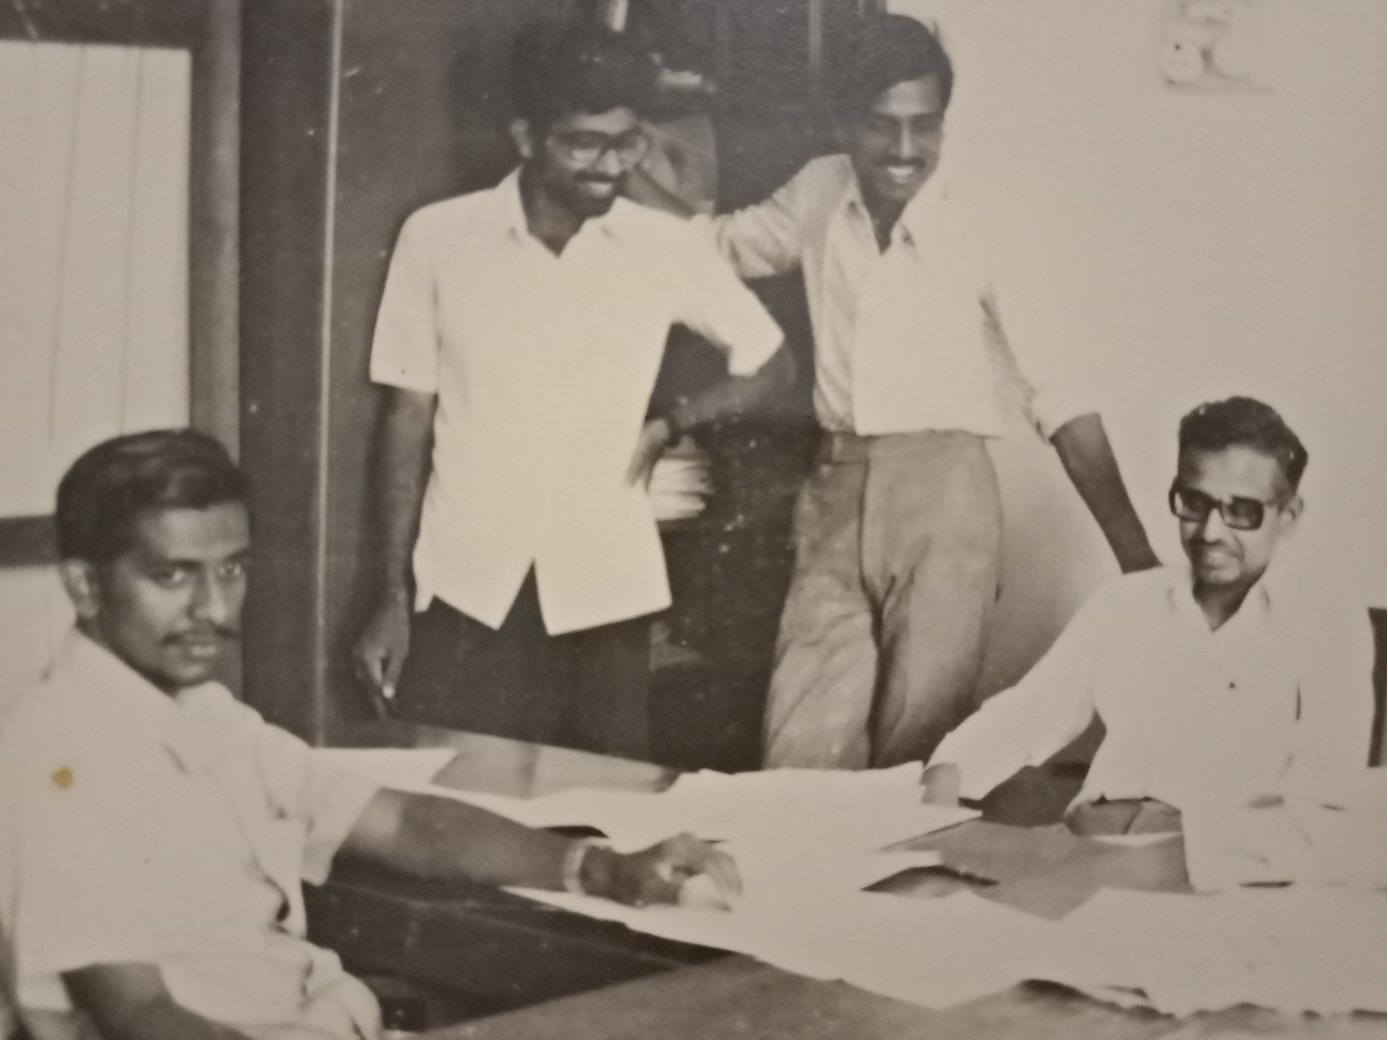
\includegraphics{images/001.jpg}
%\caption{ಲೆಕ್ಕದ ಪಟ್ಟಿ }
%\end{figure}

\begin{center}
\textbf{೧೨೫. ಮಿಸ್ಟರ್ ಜೆ.ಜೆ. ಗುಡ್ವಿನ್ ಅವರ ತಾಯಿಗೆ}
\end{center}

\begin{flushright}
(ಜೋಸಯ್ಯ ಜೆ. ಗುಡವಿನ್ ಅವರ ಅಕಾಲ ಮರಣದ ವಾರ್ತೆಯನ್ನು ಕೇಳಿ ಸ್ವಾಮಿ ವಿವೇಕಾನಂದರು ಕೆಳಗೆ ಕೊಟ್ಟಿರುವ ಪ್ಯಾರಾ ಜತೆಗೆ “ರಿಕ್ವಿಯಸ್ಕಾಟ್ ಇನ್ ಪೇಸ್”\footnote{1. ಈ ಕವನವನ್ನು ಹಿಂದೆ “ಕೃತಿಶ್ರೇಣಿ”, ಭಾಗ ೮, ಪುಟ ೩೬೪ರಲ್ಲಿ ಪ್ರಕಟಿಸಲಾಗಿದೆ.} ಎಂಬ ಕವನವನ್ನು ವೃತ್ತ ಪತ್ರಿಕೆಗಳಿಗೆ ಮತ್ತು ಗುಡ್ವಿನ್ ಅವರ ತಾಯಿಗೆ ಕಳುಹಿಸಿದರು.)
\end{flushright}

ಮಿ. ಗುಡ್ವಿನ್ ಈ ಜೀವನದಿಂದ ನಿರ್ಗಮಿಸಿದ ವ್ಯಸನಕರ ವಾರ್ತೆಯನ್ನು ಮಿತಿ ಮೀರಿದ ದುಃಖದಿಂದ ಕೇಳುತ್ತಿರುವೆನು. ಈ ವಾರ್ತೆ ಇದ್ದಕ್ಕಿದ್ದಂತೆ ಎರಗಿದುದು ದುಃಖವನ್ನು ಇನ್ನೂ ಹೆಚ್ಚು ಮಾಡಿದೆ. ಆದ ಕಾರಣ ಅವನ ಮರಣಕಾಲದಲ್ಲಿ ಅವನ ಪಕ್ಕದಲ್ಲಿರಲು ಯಾವ ರೀತಿಯಿಂದಲೂ ಸಾಧ್ಯವಾಗದೆ ಹೋಯಿತು. ಅವನ ಋಣವನ್ನು ನಾನು ಎಂದಿಗೂ ತೀರಿಸಲಾರೆ, ಯಾರು ನನ್ನ ಯಾವುದೇ ಆಲೋಚನೆಯಿಂದ ಉಪಕೃತರಾಗಿರುವರೆಂದು ಭಾವಿಸುವರೊ ಅವರು, ಅದರ ಪ್ರತಿಯೊಂದು ಪದವೂ ಮಿ. ಗುಡ್ವಿನ್ನ ಅವಿರತ ಮತ್ತು ಅತ್ಯಂತ ನಿಸ್ವಾರ್ಥ ಪರಿಶ್ರಮದಿಂದ ಪ್ರಕಟವಾಗಿದೆ ಎಂಬುದನ್ನು ತಿಳಿಯಬೇಕು. ಅವನ ನಿಧನದಿಂದ ನಾನು ಉಕ್ಕಿನಂತಹ ನೈಜ ಮಿತ್ರನನ್ನು, ಅಚಲ ನಿಷ್ಠನಾದ ಶಿಷ್ಯನನ್ನು, ಆಯಾಸವರಿಯದ ಕರ್ಮಿಯೊಬ್ಬನನ್ನು ಕಳೆದುಕೊಂಡಿದ್ದೇನೆ, ಮತ್ತು ಕೇವಲ ಇತರರಿಗಾಗಿ ಜೀವಿಸಲು ಜನ್ಮವೆತ್ತಂತಿರುವ ಕೆಲವೇ ಕೆಲವರಲ್ಲಿ ಒಬ್ಬನನ್ನು ಪ್ರಪಂಚ ಕಳೆದುಕೊಂಡು ಅದರ ಶ‍್ರೀಮಂತಿಕೆ ಕಡಿಮೆಯಾಗಿದೆ.

\begin{flushright}
(ಸಹಿ ಮಾಡಿಲ್ಲ)
\end{flushright}

\begin{center}
\textbf{೧೨೬. ಖೇತ್ರಿಯ ರಾಜರಾದ ಮಹಾರಾಜ ಅಜಿತ್ ಸಿಂಗ್ ಅವರಿಗೆ}
\end{center}

\begin{flushright}
ಶ‍್ರೀನಗರ\\ಆಗಸ್ಟ್ ೧೦, ೧೮೯೮
\end{flushright}

ಮಹಾಸ್ವಾಮಿಯವರಿಗೆ,

ಬಹಳ ಕಾಲದಿಂದ ನಿಮ್ಮಿಂದ ಯಾವ ಸಮಾಚಾರವೂ ಇಲ್ಲ. ದೈಹಿಕವಾಗಿ ಮತ್ತು ಮಾನಸಿಕವಾಗಿ ನೀವು ಹೇಗಿರುವಿರಿ?

ಶ‍್ರೀ ಅಮರನಾಥಜೀಯನ್ನು\footnote{2. ಕಾಶ್ಮೀರದ ಹಿಮಾಲಯದಲ್ಲಿನ ಒಂದು ಗುಹಾಂತರ್ದೇವಾಲಯ. ಅಲ್ಲಿ ಶಿವನ ಹಿಮಲಿಂಗವನ್ನು ಪೂಜಿಸುವರು.} ನೋಡಲು ಹೋಗಿದ್ದೆ.ಯಾತ್ರೆ ಆನಂದದಾಯಕವಾಗಿತ್ತು ಮತ್ತು ದರ್ಶನ\footnote{3. ಒಂದು ಪವಿತ್ರ ಸ್ಥಳ ಅಥವಾ ವ್ಯಕ್ತಿಗೆ ಸಾಂಪ್ರದಾಯಿಕವಾಗಿ ಹೋಗಿ ಗೌರವ ಸಲ್ಲಿಸುವುದು; ಮತ್ತು ಪವಿತ್ರತೆಯ ಸಾನ್ನಿಧ್ಯದಲ್ಲಿ ಆಶೀರ್ವಾದ ಅಥವಾ ಪರಿಶುದ್ಧತೆಯನ್ನು ಅನುಭವಿಸುವುದು. ನಿನ್ನ ಸಂಸಾರವನ್ನು ಹೇಗೆ ನಿರ್ವಹಿಸುವೆ? – ಖರ್ಚು ಮುಂತಾಗಿ? ನಿನಗೆ ಬರೆಯಲು ಇಚ್ಛೆಯಾಗುವುದನ್ನೆಲ್ಲಾ ನನಗೆ ಬರೆ. ಎಲ್ಲ ವಿಷಯಗಳನ್ನೂ ಸೇರಿಸಿ ದೀರ್ಘ ಪತ್ರವನ್ನು ಬರೆಯುವೆಯಾ? ಹಾಗೆ ಮಾಡು!} ಅದ್ಭುತವಾಗಿತ್ತು.

ನಾನು ಇಲ್ಲಿ ಇನ್ನೂ ಒಂದು ತಿಂಗಳು ಇರುತ್ತೇನೆ, ನಂತರ ಮೈದಾನ ಪ್ರದೇಶಕ್ಕೆ ಹಿಂತಿರುಗುತ್ತೇನೆ. ದಯವಿಟ್ಟು ಜಗಮೋಹನ್ ಅವರಿಗೆ, ಕಿಷನ್ಗಡದ ದಿವಾನ್ ಸಾಹೇಬರಿಗೆ ಬರೆದು, ಅವರು ಮಾತು ಕೊಟ್ಟಿದ್ದಂತೆ, ನಿಂಬಾರ್ಕ ಭಾಷ್ಯದ ಪ್ರತಿಗಳನ್ನು ನನಗೆ ತರಿಸಿಕೊಡಲು ಹೇಳಿ.

ಪೂರ್ಣ ಪ್ರೀತಿಯೊಂದಿಗೆ,

\begin{flushright}
ನಿಮ್ಮವ,\\ವಿವೇಕಾನಂದ
\end{flushright}

\begin{center}
\textbf{೧೨೭. ಸೋದರಿ ಕ್ರಿಸ್ಟೈನ್ಗೆ}
\end{center}

\begin{flushright}
ಬೇಲೂರು ಮಠ, ಹೌರಾ ಜಿಲ್ಲೆ\\ಅಕ್ಟೋಬರ್ ೨೫, ೧೮೯೮
\end{flushright}

ನನ್ನ ಪ್ರಿಯ ಕ್ರಿಸ್ಟಿನಾ,

ನೀನು ಹೇಗಿರುವೆ? ನಿನ್ನ ಆರೋಗ್ಯದ ಬಗ್ಗೆ ನನಗೆ ಬಹಳ ಆತಂಕವಾಗಿದೆ. ಬಹಳ ಕಾಲದಿಂದ ನಿನ್ನಿಂದ ನನಗೆ ಯಾವ ಪತ್ರವೂ ಬಂದಿಲ್ಲ.

ನನ್ನ ಆರೋಗ್ಯ ಮತ್ತೆ ಹಾಳಾಯಿತು. ಆದುದರಿಂದ ನಾನು ಅವಸರವಾಗಿ ಕಾಶ್ಮೀರವನ್ನು ಬಿಟ್ಟು ಕಲ್ಕತ್ತೆಗೆ ಬರಬೇಕಾಯಿತು. ಮತ್ತೆ ಈ ಚಳಿಗಾಲದಲ್ಲಿ ದೂರದ ನಡಿಗೆಯನ್ನು ಮಾಡಲೇಬಾರದೆಂದು ವೈದ್ಯರು ಹೇಳಿರುತ್ತಾರೆ. ಅದೊಂದು ದೊಡ್ಡ ನಿರಾಶೆ, ನೋಡು. ಏನೇ ಆದರೂ, ನಾನು ಈ ಬೇಸಗೆಯಲ್ಲಿ ಅಮೆರಿಕಾಕ್ಕೆ ಬರುತ್ತಿದ್ದೇನೆ. ಮಿಸೆಸ್ ಬುಲ್ ಮತ್ತು ಮಿಸ್ ಮ್ಯಾಕ್ಲಿಯಾಡ್ ಈ ವರ್ಷದ ಕಾಶ್ಮೀರ ಪ್ರವಾಸವನ್ನು ತುಂಬಾ ಆನಂದಿಸಿದರು. ಈಗ ಅವರು ಡೆಲ್ಲಿ, ಆಗ್ರ, ಜೈಪುರ್ ಮುಂತಾದ ಪ್ರದೇಶಗಳ ಪ್ರಾಚೀನ ಅವಶೇಷಗಳು ಮತ್ತು ಕಟ್ಟಡಗಳ ಕ್ಷಿಪ್ರ ಸಂದರ್ಶನ ಮಾಡುತ್ತಿರುವರು.

ನಿನಗೆ ಸಮಯವಿದ್ದರೆ ಸೊಗಸಾದ, ದೀರ್ಘವಾದ ಪತ್ರವನ್ನು ಬರೆ ಮತ್ತು ಅತಿಯಾಗಿ ಕೆಲಸ ಮಾಡಿ ಆರೋಗ್ಯವನ್ನು ಕೆಡಿಸಿಕೊಳ್ಳಬೇಡ. ಕರ್ತವ್ಯ ಕರ್ಮವನ್ನು ನಿಸ್ಸಂದೇಹವಾಗಿ ಮಾಡಲೇಬೇಕು; ಆದರೆ, ನಮಗೆ ಕರ್ತವ್ಯಗಳಿವೆ, ನಮ್ಮ ತಾಯಿ ಮುಂತಾದವರಿಗೆ ಮಾತ್ರವಲ್ಲ, ಇತರರಿಗೂ ಕೂಡ. ಕೆಲವು ವೇಳೆ ಒಂದು ಕರ್ತವ್ಯ ದೈಹಿಕ ತ್ಯಾಗವನ್ನು ಕೇಳುವುದು, ಇನ್ನೊಂದು ನಮ್ಮ ಆರೋಗ್ಯವನ್ನು ಎಚ್ಚರಿಕೆಯಿಂದ ನೋಡಿಕೊಳ್ಳಬೇಕೆಂದು ವಿಧಿಸುವುದು. ಸಹಜವಾಗಿ ನಾವು ನಮ್ಮಲ್ಲಿ ಯಾವ ಉದ್ದೇಶ ಬಲವಾಗಿದೆಯೊ ಅದನ್ನು ಅನುಸರಿಸುವೆವು. ನಿನ್ನ ವಿಷಯದಲ್ಲಿ ಯಾವುದು ಬಲವಾಗಿದೆಯೊ ನನಗೆ ಗೊತ್ತಿಲ್ಲ. ಏನೇ ಆಗಲಿ, ಈಗ ನಿನ್ನ ಸಹೋದರಿಯರು ನಿನ್ನ ನೆರವಿಗೆ ಬಂದಿರುವುದರಿಂದ ನಿನ್ನ ದೇಹವನ್ನು ಚೆನ್ನಾಗಿ ನೋಡಿಕೊ.

ನಿನ್ನ ಸಂಸಾರವನ್ನು ಹೇಗೆ ನಿರ್ವಹಿಸುವೆ? – ಖರ್ಚು ಮುಂತಾಗಿ? ನಿನಗೆ ಬರೆಯಲು ಇಚ್ಛೆಯಾಗುವುದನ್ನೆಲ್ಲಾ ನನಗೆ ಬರೆ. ಎಲ್ಲ ವಿಷಯಗಳನ್ನೂ ಸೇರಿಸಿ ದೀರ್ಘ ಪತ್ರವನ್ನು ಬರೆಯುವೆಯಾ? ಹಾಗೆ ಮಾಡು!

ದಿನೇ ದಿನೇ ನಾನು ಉತ್ತಮಗೊಳ್ಳುತ್ತಿರುವೆನು – ನಾನು ಅಮೆರಿಕಾಕ್ಕೆ ಹೊರಡಲು ಕೆಲವು ದೀರ್ಘ ತಿಂಗಳಿವೆ. ಅದೇನಾದರೂ ಆಗಲಿ, ನಮಗೆ ಯಾವುದು ಅತ್ಯಂತ ಶ್ರೇಷ್ಠವೆಂಬುದು “ತಾಯಿಗೆ” ಗೊತ್ತಿದೆ. ಅವಳು ದಾರಿ ತೋರುವಳು. ನಾನೀಗ ಭಕ್ತಿಯ ಸ್ಥಿತಿಯಲ್ಲಿರುವೆನು. ನನಗೆ ವಯಸ್ಸಾಗುತ್ತಿರುವುದರಿಂದ ಭಕ್ತಿ ಜ್ಞಾನದ ಸ್ಥಾನವನ್ನು ತೆಗೆದುಕೊಳ್ಳುತ್ತಿದೆ. ಹೊಸ “ಪ್ರಬುದ್ಧ ಭಾರತ” ನಿನಗೆ ಸಿಕ್ಕಿತೇ? ಅದು ಎಷ್ಟರ ಮಟ್ಟಿಗೆ ನಿನಗೆ ಇಷ್ಟವಾಯಿತು?

\begin{flushright}
ಭಗವಂತನಲ್ಲಿ ಎಂದಿಗೂ ನಿನ್ನವನಾದ,\\ವಿವೇಕಾನಂದ
\end{flushright}

\begin{center}
\textbf{೧೨೮. ಖೇತ್ರಿಯ ರಾಜರಾದ ಮಹಾರಾಜ ಅಜಿತ್ ಸಿಂಗ್ ಅವರಿಗೆ}
\end{center}

\begin{flushright}
ಬೇಲೂರು ಮಠ,\\ನವಂಬರ್ ೨೨, ೧೮೯೮
\end{flushright}

ಮಹಾರಾಜರೇ,

ನಿಮ್ಮ ಪತ್ರಕ್ಕಾಗಿ ಮತ್ತು ಜಗಮೋಹನ್ ಲಾಲ್ಜಿಯವರ ಮೂಲಕ ತಲಪಿದ ನಿಂಬಾರ್ಕ ಭಾಷ್ಯಕ್ಕಾಗಿ ಅನೇಕ ಧನ್ಯವಾದಗಳು.

ಇಂದು ಶ‍್ರೀ ಮಹಾರಾಜರನ್ನು ನನ್ನ ಒಂದು ಮುಖ್ಯ ಕಾರ್ಯಕ್ಕಾಗಿ – ನನ್ನ ಮನಸ್ಸನ್ನು ನಿಮ್ಮ ಮುಂದೆ ತೆರೆದಿಡಲು ಸ್ವಲ್ಪವೂ ಸಂಕೋಚವಿಲ್ಲವೆಂದು ಚೆನ್ನಾಗಿ ತಿಳಿದುಕೊಂಡಿರುವ ನಾನು – ನಿಮ್ಮನ್ನು ಕೇಳುತ್ತಿರುವೆನು. ಮತ್ತು ನಾನು ನಿಮ್ಮನ್ನು ಈ ಜೀವನದಲ್ಲಿ ನನ್ನ ಏಕೈಕ ಮಿತ್ರರೆಂದು ಪರಿಗಣಿಸುವೆನು. ಈಗ ನಾನು ತಿಳಿಸಲಿರುವುದು ನಿಮಗೆ ಸಮ್ಮತ ವೆನಿಸಿದರೆ ಒಳ್ಳೆಯದು; ಇಲ್ಲವಾದರೆ, ನನ್ನ ಮೂರ್ಖತನವನ್ನು ಸನ್ಮಿತ್ರರು ಮಾಡಬೇಕಾದಂತೆ ಕ್ಷಮಿಸಿ ಬಿಡಿ.

ನಿಮಗಾಗಲೆ ತಿಳಿದಿರುವಂತೆ, ನಾನು ಹಿಂತಿರುಗಿದಾಗಿನಿಂದ ಖಾಯಿಲೆಯಿಂದ ನರಳುತ್ತಿದ್ದೇನೆ. ಕಲ್ಕತ್ತೆಯಲ್ಲಿ ತಾವು ನನಗೆ ವೈಯಕ್ತಿಕವಾಗಿ ತಮ್ಮ ಸ್ನೇಹ ಮತ್ತು ನೆರವಿನ ಆಶ್ವಾಸನೆ ನೀಡಿದಿರಿ ಮತ್ತು ಈ ಅಪರಿಹಾರ್ಯ ಕಾಯಿಲೆಯನ್ನು ಮನಸ್ಸಿಗೆ ಹಚ್ಚಿಕೊಳ್ಳ ಬಾರದೆಂದು ತಿಳಿಯಹೇಳಿದಿರಿ. ನರಗಳ ಉದ್ರೇಕದಿಂದ ಈ ಕಾಯಿಲೆ ಬಂದಿರುವುದು; ಎಷ್ಟೇ ಸ್ಥಳ ಬದಲಾವಣೆ ಮಾಡಿದರೂ, ಚಿಂತೆ ಆತಂಕ ಉದ್ರೇಕಗಳನ್ನು ನನ್ನಿಂದ ತೆಗೆದು ಹಾಕಿದ ಹೊರತು ಪ್ರಯೋಜನವಿಲ್ಲ.

ಈ ಎರಡು ವರ್ಷಗಳು ಹವಾ ಬದಲಾವಣೆಯನ್ನು ಪ್ರಯತ್ನಿಸಿದ ಮೇಲೆ, ನನ್ನ ಆರೋಗ್ಯ ದಿನೇ ದಿನೇ ಕೆಡುತ್ತಿದೆ ಮತ್ತು ಈಗ ಮೃತ್ಯುದ್ವಾರಕ್ಕೆ ಹತ್ತಿರ ಬಂದಿದೆ. ನಾನು ಮಹಾರಾಜರ ಕೆಲಸ, ಔದಾರ್ಯ ಮತ್ತು ಸ್ನೇಹಕ್ಕೆ ವಿನಂತಿಸಿಕೊಳ್ಳುತ್ತಿದ್ದೇನೆ. ನನ್ನ ಎದೆಯಲ್ಲಿ ಒಂದು ಪಾಪ ಸದಾ ಕೊರೆಯುತ್ತಿದೆ. ಅದೇನೆಂದರೆ, ಪ್ರಪಂಚಕ್ಕೆ ಒಂದು ಸೇವೆಯನ್ನು ಮಾಡುವುದು. ನಾನು ನನ್ನ ತಾಯಿಯನ್ನು ಬಹಳ ಉದಾಸೀನಮಾಡಿ ಬಿಟ್ಟಿದ್ದೇನೆ. ಮತ್ತೆ, ನನ್ನ ಎರಡನೆಯ ಸೋದರ ಕಾಲವಾದ ಮೇಲೆ ಆಕೆ ದುಃಖದಲ್ಲಿ ಬಹಳ ನವೆದುಹೋಗಿರುವಳು. ಈಗ ನನ್ನ ಕೊನೆಯ ಆಸೆಯೆಂದರೆ, ಸೇವೆಯನ್ನು ಮಾಡುವುದು ಮತ್ತು ನನ್ನ ತಾಯಿಗೆ ಕೆಲವು ವರ್ಷಗಳಾದರೂ ಸೇವೆ ಮಾಡುವುದು. ನಾನು ನಮ್ಮ ತಾಯಿಯೊಂದಿಗೆ ಇದ್ದು, ವಂಶ ನಾಶವಾಗದಂತೆ ನನ್ನ ತಮ್ಮನಿಗೆ ವಿವಾಹ ಮಾಡಿಸಬೇಕೆಂದಿದ್ದೇನೆ. ಇದು ಖಂಡಿತವಾಗಿ ನನ್ನ ಹಾಗೂ ನನ್ನ ತಾಯಿಯ ಕಡೆಯ ದಿನಗಳನ್ನು ಹಗುರಗೊಳಿಸುವುದು. ಈಗ ಅವಳು ವಾಸಯೋಗ್ಯವಲ್ಲದ ಮುರುಕಲು ಮನೆಯಲ್ಲಿರುವಳು. ನಾನೀಗ ಆಕೆಗಾಗಿ ಒಂದು ಸಣ್ಣದಾದ, ಚೊಕ್ಕವಾದ ಮನೆಯನ್ನು ಕಟ್ಟಿ ಕಿರಿಯವನಿಗೂ ಅದರಲ್ಲಿ ಒಂದು ಜಾಗ ಮಾಡಬೇಕೆಂದಿರುವೆನು, ಏಕೆಂದರೆ ಅವನು ಹೆಚ್ಚಾಗಿ ಹಣ ಸಂಪಾದಿಸುವ ಸಂಭವ ಕಡಿಮೆ. ರಾಮಚಂದ್ರನ ರಾಜ ವಂಶಜರಿಗೆ ತಾವು ಪ್ರೀತಿಸುವ ಮತ್ತು ತಮ್ಮ ಮಿತ್ರರೆಂದು ಕರೆಯುವವರಿಗೆ ಮಾಡಲು ಇದು ಹೆಚ್ಚಾಗುವುದೇ? ಮತ್ತಾರನ್ನು ಕೇಳಿಕೊಳ್ಳಬೇಕೊ ನನಗೆ ಗೊತ್ತಾಗುವುದಿಲ್ಲ. ಯೂರೋಪ್ನಿಂದ ನನಗೆ ದೊರೆತ ಹಣ “ಕಾರ್ಯ”ಕ್ಕಾಗಿ, ಮತ್ತು ಪ್ರತಿಯೊಂದು ಪೆನ್ನಿಯೂ ಕೂಡ ಆ ಕಾರ್ಯಕ್ಕಾಗಿ ಕೊಡಲಾಗಿದೆ. ಸಹಾಯಕ್ಕಾಗಿ ಮತ್ತು ನನಗಾಗಿ ನಾನು ಮತ್ತಾರನ್ನೂ ಬೇಡಲಾರೆ. ನನ್ನ ಸಂಸಾರದ ವಿಷಯವಾಗಿ – ಎಲ್ಲವನ್ನೂ ತಮಗೆ ಬಿಚ್ಚಿ ಹೇಳಿರುತ್ತೇನೆ, ಮತ್ತು ಯಾರಿಗೂ ಈ ವಿಷಯ ತಿಳಿಯದಿರಲಿ. ನನಗೆ ಸಾಕಾಗಿದೆ, ನಾನು ಬೇಸತ್ತಿರುವೆ ಮತ್ತು ಸಾಯುತ್ತಿರುವೆನು. ತಮ್ಮ ಘನತೆ ಮತ್ತು ಔದಾರ್ಯಕ್ಕೆ ತಕ್ಕುದಾದ ಮತ್ತು ನನಗೆ ತಾವು ತೋರಿರುವ ಅನೇಕ ಔದಾರ್ಯಗಳಿಗೆ ಮಕುಟಪ್ರಾಯವಾದ ಈ ಕಡೆಯದಾದ ಕರುಣೆಯ ಮಹತ್ಕಾರ್ಯವನ್ನು ದಯವಿಟ್ಟು ಮಾಡುವುದು. ನನ್ನ ಕೊನೆಯ ದಿನಗಳನ್ನು ನೀವು ಹಗುರ ಮತ್ತು ಸುಲಭ ಮಾಡುತ್ತಿರುವಂತೆ ಯಾರಿಗೆ ಇಡಿ ಜೀವನ ಸೇವೆ ಗೈಯಲು ನಾನು ಯತ್ನಿಸಿರುವೆನೊ ಅವನು ತನ್ನ ಶ್ರೇಷ್ಠವಾದ ಆಶೀರ್ವಾದಗಳನ್ನು ತಮ್ಮ ಮೇಲೆ ಮತ್ತು ತಮ್ಮವರ ಮೇಲೆ ಸದಾ ವರ್ಷಿಸಲಿ.

\begin{flushright}
ಭಗವಂತನಲ್ಲಿ ಎಂದಿಗೂ ನಿನ್ನವನಾದ,\\ವಿವೇಕಾನಂದ
\end{flushright}

ವಿ.ಸೂ.: ಇದು ಕಡ್ಡಾಯವಾಗಿ ವೈಯಕ್ತಿಕವಾದುದು. ತಾವು ಇದನ್ನು ಮಾಡುವಿರೊ ಇಲ್ಲವೊ ಎಂಬುದರ ಬಗ್ಗೆ ನನಗೆ ದಯವಿಟ್ಟು ತಂತಿ ಸಂದೇಶ ಕಳುಹಿಸುವಿರಾ?

\begin{flushright}
ಎಂದಿಗೂ ನಿಮ್ಮವ,\\ವಿವೇಕಾನಂದ
\end{flushright}

\begin{center}
\textbf{೧೨೯. ಖೇತ್ರಿಯ ರಾಜರಾದ ಮಹಾರಾಜ ಅಜಿತ್ ಸಿಂಗ್ ಅವರಿಗೆ}
\end{center}

\begin{flushright}
ಬೇಲೂರು ಮಠ, ಹೌರಾ ಜಿಲ್ಲೆ\\ಡಿಸೆಂಬರ್ ೦೧, ೧೮೯೮
\end{flushright}

ಮಹಾರಾಜರೇ,

ನಿಮ್ಮ ತಂತಿ ಸಮಾಚಾರ ನನಗೆ ಹೇಳಲಾಗದಷ್ಟು ಸಂತೋಷವುಂಟುಮಾಡಿದೆ, ಮತ್ತು ಅದು ನಿಮ್ಮ ಘನತೆಗೆ ತಕ್ಕಂತಿದೆ. ನನಗೆ ಬೇಕಾದುದರ ಪಟ್ಟಿಯನ್ನು ಇದರೊಂದಿಗೆ ಕೊಟ್ಟಿರುವೆನು. ಕಲ್ಕತ್ತೆಯಲ್ಲಿ ಒಂದು ಸಣ್ಣ ಮನೆಯನ್ನು ಕಟ್ಟಲು ಅಂದಾಜು ಕನಿಷ್ಠ ಹತ್ತು ಸಾವಿರ ರೂಪಾಯಿಗಳು. ಆ ಹಣದಿಂದ ಯಾವುದೊ ಒಂದು ಮೂಲೆಯಲ್ಲಿ ಹೇಗೊ ಒಂದು ಮನೆಯನ್ನುಕೊಳ್ಳಬಹುದು ಅಥವಾ ಕಟ್ಟಬಹುದು – ನಾಲ್ಕೈದು ಜನರು ವಾಸಿಸುವ ಸಣ್ಣ ಮನೆ. ಜೀವನದ ಖರ್ಚಿಗೆ, ಉದಾರವಾಗಿ ಪ್ರತಿ ತಿಂಗಳೂ ನೀವು ನಮ್ಮ ತಾಯಿಗೆ ಕಳುಹಿಸುತ್ತಿರುವ ರೂ. ೧೦೦ ಆಕೆಗೆ ಸಾಕಾಗುತ್ತದೆ. ಇದರ ಜತೆಗೆ ನೀವು ತಿಂಗಳೊಂದಕ್ಕೆ ನನ್ನ ಜೀವಿತಾವಧಿಯವರೆಗೆ ೧೦೦ ರೂ.ಗಳನ್ನು ಸೇರಿಸಿದರೆ–ನನಗೆ ಬಹಳ ಸಂತೋಷ. ದುರದೃಷ್ಟದಿಂದ ಈ ಕಾಯಿಲೆ ಅದನ್ನು ಹೆಚ್ಚಿಸಿದೆ, ಮತ್ತು ಅದು ಹೆಚ್ಚು ಕಾಲ ನಿಮಗೆ ತೊಂದರೆಗೆ ಕಾರಣವಾಗದೆಂದು ಭಾವಿಸುವೆ, ಏಕೆಂದರೆ ನಾನು ಕೆಲವು ವರ್ಷಗಳು ಮಾತ್ರ ಬದುಕುವೆನೆಂದು ನನ್ನ ನಿರೀಕ್ಷೆ. ಮತ್ತೊಂದನ್ನು ನಾನು ನಿಮ್ಮಲ್ಲಿ ಕೇಳಿಕೊಳ್ಳುತ್ತೇನೆ – ಸಾಧ್ಯವಾದರೆ, ನೀವು ಪ್ರತಿ ತಿಂಗಳು ನಮ್ಮ ತಾಯಿಗೆ ಕೊಡುತ್ತಿರುವ ರೂ. ೧೦೦ನ್ನು ನನ್ನ ಕಾಲಾನಂತರವೂ ತಪ್ಪದೆ ಅವಳಿಗೆ ತಲುಪುವಂತೆ ಖಾಯಂಗೊಳಿಸಿ. ನನ್ನ ಮೇಲಿನ ಪ್ರೀತಿ ಮತ್ತು ಕರುಣೆಯನ್ನು ನಿಲ್ಲಿಸಲು ತಮಗೆ ಎಂದಾದರೂ ಕಾರಣಗಳು ದೊರೆತರೆ, ಹಿಂದೊಮ್ಮೆ ಒಬ್ಬ ಬಡ ಸಾಧುವಿನ ಮೇಲೆ ನಿಮಗಿದ್ದ ಪ್ರೀತಿಯನ್ನು ನೆನಪು ಮಾಡಿಕೊಂಡು ನನ್ನ ವೃದ್ಧ ಬಡ ತಾಯಿಗೆ ನಿಮ್ಮ ಸಹಾಯ ದೊರೆಯಲಿ.

ಇಷ್ಟೆ. ನೀವು ಮಾಡಿರುವ ಅನೇಕ ಇತರ ಘನ ಕಾರ್ಯಗಳ ಜತೆಗೆ ಈ ಸಣ್ಣ ಕಾರ್ಯವನ್ನು ಮಾಡಿ ಮತ್ತೇನನ್ನಾದರೂ ಸಾಬೀತು ಮಾಡಲು ಸಾಧ್ಯವೊ ಅಲ್ಲವೊ, ಕರ್ಮದ ಶಕ್ತಿ ಸ್ವಯಂ ವಿದಿತ ಎಂಬುದನ್ನು ಚೆನ್ನಾಗಿ ತಿಳಿದು ಮಾಡಿ. ಈ ಒಳ್ಳೆಯ ಕರ್ಮದ ಅನುಗ್ರಹ ನಿಮ್ಮನ್ನು ಮತ್ತು ನಿಮ್ಮವರನ್ನು ಸದಾ ಹಿಂಬಾಲಿಸುವುದು. ನನ್ನ ವಿಷಯವಾಗಿ, ಏನು ಹೇಳಲಿ – ನಾನು ಈ ಪ್ರಪಂಚದಲ್ಲಿ ಏನಾಗಿರುವೆನೊ ಅದೆಲ್ಲಾ ಬಹುತೇಕ ನಿಮ್ಮ ಸಹಾಯದಿಂದ. ಒಂದು ದೊಡ್ಡ ಆತಂಕದಿಂದ ಪಾರಾಗಿ ಮತ್ತು ಪ್ರಪಂಚವನ್ನು ಎದುರಿಸಿ ಸ್ವಲ್ಪ ಕೆಲಸವನ್ನು ಮಾಡಲು ಸಾಧ್ಯವಾಗುವಂತೆ ನೀವು ಮಾಡಿದಿರಿ. ನನ್ನ ಮನಸ್ಸಿನಿಂದ ಈ ಹೊರೆಯನ್ನು ಮತ್ತೊಮ್ಮೆ ತೆಗೆದು ಹಾಕಿ ಭಗವಂತನ ನಿಮಿತ್ತವಾಗಿ ಇನ್ನೂ ಭವ್ಯವಾದ ಕೆಲಸಕ್ಕೆ ನೀವು ನಿಯೋಜಿಸಲ್ಪಟ್ಟಿರುವಿರಿ.

ಆದರೆ ನೀವು ಇದನ್ನು ಮಾಡುವಿರೊ ಇಲ್ಲವೊ, “ಒಮ್ಮೆ ಪ್ರೀತಿಸಲ್ಪಡುವವರು ಸದಾ ಪ್ರೀತಿಪಾತ್ರರು.” ನನ್ನ ಎಲ್ಲ ಪ್ರೀತಿ ಮತ್ತು ಆಶೀರ್ವಾದಗಳು ಮತ್ತು ಪ್ರಾರ್ಥನೆಗಳು ನಿಮ್ಮನ್ನೂ ಮತ್ತು ನಿಮ್ಮವರನ್ನೂ ಹಿಂಬಾಲಿಸಲಿ, ಹಗಲು ಮತ್ತು ರಾತ್ರಿ, ಯಾವುದಕ್ಕೆ ನಾನು ನಿಮಗಾಗಲೆ ಋಣಿಯಾಗಿರುವೆನೊ ಅದಕ್ಕಾಗಿ ಹಿಂಬಾಲಿಸಲಿ; ಮತ್ತು ಈ ಸೃಷ್ಟಿ ಯಾರ ಕ್ರೀಡೆಯೊ ಮತ್ತು ಯಾರ ಕೈಗಳಲ್ಲಿ ನಾವು ಕೇವಲ ಯಂತ್ರಗಳೊ ಅಂತಹ ಭಗವತಿ ನಿಮ್ಮ ಎಲ್ಲಾ ಅನಿಷ್ಟಗಳಿಂದಲೂ ಸದಾ ರಕ್ಷಿಸಲಿ.

\begin{flushright}
ಭಗವಂತನಲ್ಲಿ ಎಂದಿಗೂ ನಿಮ್ಮವನಾದ,\\ವಿವೇಕಾನಂದ
\end{flushright}

\begin{center}
\textbf{೧೩೦. ಸೋದರಿ ನಿವೇದಿತಾಳಿಗೆ}
\end{center}

\begin{flushright}
ಮಧ್ಯಾಹ್ನ ೩ ಗಂಟೆ, ಭಾನುವಾರ\\೧೮೯೯ರ ಮೊದಲ ಭಾಗ
\end{flushright}

ನನ್ನ ಪ್ರಿಯ ಮಾರ್ಗಾಟ್,

ಡಾ. ಮಹಾನೆಯವರನ್ನು\footnote{1. ಡಾ. ಮಹಾನೆ ಜಿಲ್ಲೆಯ ವೈದ್ಯಾಧಿಕಾರಿಗಳು. ೧೮೯೯ರ ಆದಿ ಭಾಗದಲ್ಲಿ ರಾಮಕೃಷ್ಣ ಮಿಷನ್ನವರು ಸೋದರಿ ನಿವೇದಿತೆಯ ನಾಯಕತ್ವದಲ್ಲಿ ಕಲ್ಕತ್ತೆಯಲ್ಲಿ ಮಾಡಿದ ಪ್ಲೇಗ್ ನಿವಾರಣಾ ಕಾರ್ಯದಲ್ಲಿ ಚರಂಡಿ ಕೆಲಸಗಳ ಮೇಲ್ವಿಚಾರಣೆಯನ್ನು ಮಾಡುತ್ತಿದ್ದರು.} ನೋಡಲು ಬರಲಾಗದುದಕ್ಕೆ ನನಗೆ ವಿಷಾದವಾಗುತ್ತದೆ – ನನಗೆ ಕಾಯಿಲೆಯಾಗಿದೆ. ನನ್ನ ಉಪವಾಸವನ್ನು ಇನ್ನೂ ಮುಗಿಸಿಲ್ಲ.

ನನ್ನ ಕಿರಿಯ ದಾಯಾದಿಗೆ ಪಾಠ ಹೇಳಿಕೊಡುವುದನ್ನು ನಿಲ್ಲಿಸಿ ಬಿಟ್ಟೆಯಾ?

\begin{flushright}
ಪ್ರೀತಿಯಿಂದ ನಿನ್ನವ,\\ವಿವೇಕಾನಂದ
\end{flushright}

\begin{center}
\textbf{೧೩೧. ಸೋದರಿ ನಿವೇದಿತಾಳಿಗೆ}
\end{center}

\begin{flushright}
(೧೮೯೯ ಮೊದಲ ಭಾಗ?)
\end{flushright}

ನನ್ನ ಪ್ರಿಯ ನಿವೇದಿತಾ,

ನನ್ನ ದಾಯಾದಿಯ ವಿಳಾಸ ೧೨೭ ಮಾಣಿಕ್ ತಾಲಾ ಬೀದಿ. ಗಂಡನ ಹೆಸರು ದುರ್ಗಾ ಪ್ರಸನ್ನ ಬೋಸ್. ಹೆಂಡತಿಯ ಹೆಸರು ಬಹುಶಃ ನೀನು ಭೇಟಿ ಮಾಡುವ ಯಾವ ಗಂಡನಿಗೂ ಗೊತ್ತಿರುವುದಿಲ್ಲ. ಆದುದರಿಂದ ಇಂತಹವರ ಹೆಂಡತಿ ಎಂದು ಕೇಳಿಕೊಂಡು ಹೋಗುವುದು ಪದ್ಧತಿ.

ಮಾಣಿಕ್ ತಾಲ ಬೀದಿ ಕೆರೆ ಇರುವ ತೋಟದಿಂದ ದಕ್ಷಿಣಕ್ಕೆ ಪೂರ್ವ – ಪಶ್ಚಿಮವಾಗಿ ಹೋಗುವುದು.

\begin{center}
\textbf{೧೩೨. ಸೋದರಿ ಕ್ರಿಸ್ಟೈನ್ ಗೆ}
\end{center}

\begin{flushright}
ಬೇಲೂರು ಮಠ, ಹೌರಾ ಜಿಲ್ಲೆ, ಬಂಗಾಲ, ಭಾರತ\\ಜನವರಿ ೨೬, ೧೮೯೯
\end{flushright}

ನನ್ನ ಪ್ರಿಯ ಕ್ರಿಸ್ಟಿನಾ,

ನಿನ್ನ ಬಹು ಸುಂದರವಾದ ಪತ್ರಕ್ಕೆ ಉತ್ತರ ಬರೆಯಲು ಇಷ್ಟೊಂದು ತಡವಾದುದಕ್ಕೆ ಕ್ಷಮಿಸು. ನಿಜಾಂಶವೇನೆಂದರೆ, ನಾನು ಮತ್ತೊಮ್ಮೆ ಸಾವಿನ ಕಣಿವೆಯಲ್ಲಿದ್ದೆ. ಹಳೆಯ ಡಯಾಬಿಟೀಸ್ ಈಗ ಮಾಯವಾಗಿದೆ. ಅದರ ಜಾಗದಲ್ಲಿ, ಕೆಲವು ವೈದ್ಯರು ಕರೆಯುವ ಅಸ್ತಮ, ಮತ್ತೆ ಕೆಲವರು ಕರೆಯುವ ಡಿಸ್ಪೆಪ್ಸಿಯಾ ಎಂಬುದು ನರಗಳ ದೌರ್ಬಲ್ಯದಿಂದ ಬಂದಿವೆ. ಅದೇನೇ ಇರಲಿ, ಅದೊಂದು ಉಸಿರು ಕಟ್ಟುವಂತೆ ಮಾಡುವ, ಕೆಲವು ವೇಳೆ ಕೆಲವು ದಿನಗಳವರೆಗೆ ಅತ್ಯಂತ ತೊಂದರೆ ಕೊಡುವ ಕಾಯಿಲೆ. ನನ್ನ ಆರೋಗ್ಯ ಉತ್ತಮವಾಗಿರುವುದು ಕಲ್ಕತ್ತೆಯಲ್ಲಿ ಮಾತ್ರ; ಆದುದರಿಂದ ನಾನು ವಿಶ್ರಾಂತಿ ಮತ್ತು ಸರಳ ಆಹಾರಕ್ಕಾಗಿ ಇಲ್ಲಿ ಇರುವೆನು. ಮಾರ್ಚ್ ತಿಂಗಳ ಸಮಯಕ್ಕೆ ನಾನು ಗುಣಮುಖವಾದರೆ ಯೂರೋಪ್ಗೆ ಹೊರಡುವೆನು. ಮಿಸೆಸ್ ಬುಲ್ ಮತ್ತು ಇತರರು ಭಾರತದಿಂದ ಹೋದರು; ಈ ಕಾಯಿಲೆಯಿಂದಾಗಿ ನಾನು ಅವರೊಡನೆ ಹೋಗಲಾಗ ದುದಕ್ಕೆ ವಿಷಾದಿಸುತ್ತೇನೆ.

ನೀನು ಇಲ್ಲಿಗೆ ಬರುವ ನಿನ್ನ ಯೋಜನೆಯ ಆಗುಹೋಗುಗಳನ್ನು ಎಚ್ಚರಿಕೆಯಿಂದ ಪರಿಶೀಲಿಸಿದ್ದೇನೆ. ನೀನು ಬಂದರೆ ನನಗೆ ಬಹಳ ಸಂತೋಷ. ಅದು ನಿನಗೆ ಚೆನ್ನಾಗಿ ಗೊತ್ತಿದೆ; ಆದರೆ, ಪ್ರಿಯ ಕ್ರಿಸ್ಟಿನಾ, ಭಾರತದ ಬೇಸಗೆ ನಿನಗೆ ಸರಿಹೋಗದು, ಮತ್ತು ನೀನು ಈಗ ಹೊರಟರೆ, ನೀನು ಭಾರತವನ್ನು ತಲುಪುವ ಸಮಯಕ್ಕೆ ಬೇಸಗೆಯ ಮಧ್ಯ ಕಾಲವಾಗುವುದು. ಆಗ ನೀನು ಇಲ್ಲಿ ವಾಸಿಸಲಾಗುವುದಿಲ್ಲ. ಅನೇಕ ವೇಳೆ ನನ್ನ ದೇಶದಲ್ಲಿಯೇ ನನಗೆ ವಾಸಿಸಲು ಅಸಾಧ್ಯವಾಗುವುದು. ಆಗ ಇಲ್ಲಿಸುತ್ತಮುತ್ತ ಪರಿಸ್ಥಿತಿ ಬಹಳ ಕೆಡುವುದು ಮತ್ತು ನಿಮ್ಮಲ್ಲಿ ಇರುವುದಕ್ಕಿಂತ ಬಹಳ ಬೇರೆಯಾಗಿರುವುದು. ಉದಾಹರಣೆಗೆ ನಾನು ಕೌಪೀನ ಮಾತ್ರ ಧರಿಸಿ ಓಡಾಡಬೇಕಾಗುವುದು – ಅದು ನಿನಗೆ ದಿಗ್ಭ್ರಮೆ ಉಂಟು ಮಾಡುವುದೇ? ಮುಕ್ಕಾಲು ಪಾಲು ಜನರು ಸೊಂಟಕ್ಕೆ ಬಿಳಿ ಬಟ್ಟೆಯ ತುಂಡನ್ನುಸುತ್ತಿಕೊಂಡು ಓಡಾಡುವರು – ಅದು ನಿನಗೆ ಸಹಿಸಲಾಗುವುದೇ?

ನಾನು ಇಲ್ಲಿಗೆ ನಿಲ್ಲಿಸಬೇಕು; ಬಹಳ ದುರ್ಬಲನಾಗಿರುವೆನು. ಮಾರ್ಚ್ ಸಮಯಕ್ಕೆ ನಾನು ಗುಣಮುಖವಾಗದಿದ್ದರೆ, ಇಲ್ಲಿಗೆ ಬರಲು ನಾನು ಬರೆಯುವೆ, ಏಕೆಂದರೆ ನಾನು ಕಾಲವಾಗುವುದಕ್ಕೆ ಮುಂಚೆ ನಿನ್ನನ್ನು ಒಮ್ಮೆ ನೋಡಬೇಕೆಂದು ನನಗೆ ಬಹಳ ಇಚ್ಛೆ ಯಿದೆ.

ಚಿಂತಿಸಬೇಡ, ಪ್ರಿಯ ಕ್ರಿಸ್ಟಿನಾ. “ತಾಯಿ” ಇಚ್ಛಿಸಿದಂತೆ ನಡೆಯಬೇಕು. ನಮ್ಮ ದೇನಿದ್ದರೂ ವಿಧೇಯರಾಗಿದ್ದು ಕೆಲಸ ಮಾಡುವುದು.

\begin{flushright}
ಭಗವಂತನಲ್ಲಿ ಎಂದಿಗೂ ನಿನ್ನವನಾದ,\\ವಿವೇಕಾನಂದ
\end{flushright}

ವಿ.ಸೂ.: ಮಿಸೆಸ್ ಬುಲ್ ಕೇಂಬ್ರಿಜ್, ಮಸಾಚುಸೆಟ್ಸ್ ಅನ್ನು ಶೀಘ್ರವೇ ಸೇರಲಿರುವರು. ವಿವರಗಳಿಗಾಗಿ ನೀನು ಅಲ್ಲಿಗೆ ಬರೆಯಬಹುದು.

\begin{flushright}
ನಿನ್ನವ,\\ವಿವೇಕಾನಂದ
\end{flushright}

ವಿ.ವಿ.ಸೂ.: ನಿನ್ನ ವಿಳಾಸ ಮತ್ತೆ ಕಳೆದು ಹೋಗಿದೆ. ದಯವಿಟ್ಟು ಸರಿಯಾದ ವಿಳಾಸವನ್ನು ಮುಂದಿನ ಪತ್ರದಲ್ಲಿ ಬರೆ.

\begin{flushright}
ವಿವೇಕಾನಂದ
\end{flushright}

\begin{center}
\textbf{೧೩೩. ಸ್ವಾಮಿ ಬ್ರಹ್ಮಾನಂದರಿಗೆ}
\end{center}

\begin{flushright}
ಬೇಲೂರು ಮಠ\\ಶುಕ್ರವಾರ ಮಾರ್ಚ್ (?), ೧೮೯೯
\end{flushright}

ನನ್ನ ಪ್ರಿಯ ರಾಜ,

ದಯವಿಟ್ಟು ಸೋದರಿ ನಿವೇದಿತಳಿಗೆ ರೂ. ೧೦೦ನ್ನು ಪ್ಲೇಗ್ ಕೆಲಸಕ್ಕಾಗಿ ಕೂಡಲೆ ಕೊಡು ಮತ್ತು ಅದನ್ನು ಪ್ರತ್ಯೇಕವಾದ ಪ್ಲೇಗ್ ಲೆಕ್ಕಕ್ಕೆ ಸೇರಿಸು.

\begin{flushright}
ವಿಶ್ವಾಸಪೂರ್ವಕವಾಗಿ ನಿನ್ನವ,\\ವಿವೇಕಾನಂದ
\end{flushright}

\begin{center}
\textbf{೧೩೪. ಸ್ವಾಮಿ ಸ್ವರೂಪಾನಂದರಿಗೆ,\\“ಪ್ರಬುದ್ಧ ಭಾರತ” ದ ಸಂಪಾದಕರು, ಮಾಯಾವತಿ}
\end{center}

\begin{flushright}
ಮಾರ್ಚ್ ೧೮೯೯
\end{flushright}

ನನ್ನ ಪ್ರಿಯ ಎಸ್. (ಸ್ವರೂಪಾನಂದ),

ನನ್ನ ಹೆಸರಿನ ಮೇಲೆ ಮಿಸೆಸ್ ಸೇವಿಯರ್ ಅವರ ಹೆಸರು ಬರುವುದೊ ಅಥವಾ ಮತ್ತಾರದೊ ಬರುವುದೊ, ಅದಕ್ಕೆ ನನ್ನ ಆಕ್ಷೇಪಣೆ ಇಲ್ಲ; ಕೈಪಿಡಿ ಸೇವಿಯರ್ ದಂಪತಿಗಳ ಹೆಸರಿನಲ್ಲಿ ಇರಬೇಕು. ಆವಶ್ಯಕತೆ ಇದ್ದರೆ, ನನ್ನ ಹೆಸರನ್ನು ಸೇರಿಸು. ಕೈ ಪಿಡಿಯಲ್ಲಿ ಸೇರಿಸಲು ನಿನ್ನ ಅವಗಾಹನೆಗಾಗಿ ಕೆಲವು ವಾಕ್ಯಗಳನ್ನು\footnote{1. ಸ್ವಾಮಿ ವಿವೇಕಾನಂದರು ಬರೆದ ಕೈ ಪಿಡಿಯ ಕರಡನ್ನು “ಕೃತಿ ಶ್ರೇಣಿ” ನಂ. ೫, ಪು. ೩೮೦ರಲ್ಲಿ ನೋಡಿ.} ಕಳುಹಿಸುತ್ತಿದ್ದೇನೆ.

ಕರಾರಿನ ಕರಡನ್ನು ಶೀಘ್ರವೇ ಕಳುಹಿಸುತ್ತೇನೆ.

\begin{flushright}
ವಿವೇಕಾನಂದ
\end{flushright}

\begin{center}
\textbf{೧೩೫. ಸೋದರಿ ನಿವೇದಿತಾಗೆ}
\end{center}

\begin{flushright}
ಬೇಲೂರು ಮಠ,\\ಮಾರ್ಚ್ ೦೨, ೧೮೯೯
\end{flushright}

ನನ್ನ ಪ್ರಿಯ ಮಾರ್ಗಾಟ್,

ನಿನ್ನ ಪೆಟ್ಟಿಗೆಗಳಲ್ಲಿ ನನ್ನದೊಂದು ಸಂಸ್ಕೃತದ ಪುಸ್ತಕವಿದೆಯೆ ಎಂದು ನೋಡು ವೆಯಾ? ಅದು, ನಿನಗೆ ಗೊತ್ತಿರುವಂತೆ, ಕಾಶ್ಮೀರದಲ್ಲಿ ನಿನ್ನಲ್ಲಿತ್ತು. ಅದು ನಮ್ಮ ಗ್ರಂಥಾಲಯದಲ್ಲಿ ಕಾಣುತ್ತಿಲ್ಲ.

ನಿನ್ನ ಸ್ನೇಹಿತೆ ಮಿಸ್ (ಸರಳ) ಘೋಷಾಲ್ ಭಾನುವಾರ ಮಠವನ್ನು ನೋಡಲು ಬರುವುದನ್ನು ಕುರಿತು ಯೋಚಿಸುತ್ತಿದ್ದೆ. ಒಂದು ಸಮಸ್ಯೆ ಇದೆ. ಸಂಜೆ ೫ ಗಂಟೆಯವರೆಗೆ ನದಿಯಲ್ಲಿ ನೀರು ಇಳಿಮುಖವಾಗುವುದು. ಆಗ ನಮ್ಮ ದೊಡ್ಡ ದೋಣಿ ಸರಾಗವಾಗಿ ನೀರಿನಲ್ಲಿ ಇಳಿದು ಹೋಗಿ ತಂಡವನ್ನು ಕರೆದುಕೊಂಡು ಬರಬಹುದು; ಮತ್ತು ಹಿಂತಿ ರುಗುವಾಗ, ಅವರು ಸಂಜೆ ೫ ಗಂಟೆಗೆ ಮುಂಚೆಯೇ ಹೊರಟರೆ, ೪ ಗಂಟೆ ಎಂದಿಟ್ಟು ಕೊಳ್ಳಿ, ಅದು ಸರಿಹೋಗುವುದು. ಮೇಲಕ್ಕೆ ಬರಲು ಬಾಗ್ಬಜಾರಿನಿಂದ ಕನಿಷ್ಠ ಎರಡು ಗಂಟೆ ಆಗುವುದು. ತಂಡ ಮಧ್ಯಾಹ್ನ ೧೨ಕ್ಕೆ ಬಾಗ್ ಬಜಾರ್ನಿಂದ ಹೊರಟು ೨ ಗಂಟೆಗೆ ಮಠಕ್ಕೆ ಊಟಕ್ಕೆ ಬಂದರೆ ಮತ್ತು ಸಂಜೆ ೪ ಗಂಟೆಗೆ ಹಿಂತಿರುಗಿ ಹೊರಟರೆ ಒಳ್ಳೆಯದು.

ನೀವು ಅಷ್ಟು ಬೇಗನೆ ಹೊರಡಲು ಆಗದೆ ಇದ್ದರೆ, ನೀನು ಗಾಡಿಯನ್ನು ಬಾರಾ ನಗರದ ಹತ್ತಿರ ಆಚೆ ದಡದಲ್ಲಿ ಕಾಯಲು ಹೇಳುವುದು ಸೂಕ್ತ. ಆಗ ನಾವು ಜನರನ್ನು ದೋಣಿಯಲ್ಲಿ ಅವರಿಗೆ ಯಾವ ಸಮಯ ಸರಿಹೋಗುವುದೊ ಆಗ ಕರೆದುಕೊಂಡು ಬರಬಹುದು. ಹಾಗಿದ್ದರೆ ದೋಣಿ ಪ್ರಯಾಣ ಬರುವಾಗ ಮಾತ್ರ.

\begin{flushright}
ಪೂರ್ಣ ಪ್ರೀತಿ ಮತ್ತು ಆಶೀರ್ವಾದಗಳೊಂದಿಗೆ,\\ವಿವೇಕಾನಂದ
\end{flushright}

\begin{center}
\textbf{೧೩೬. ಈಶ್ವರಚಂದ್ರ ಘೋಷ್ ಅವರಿಗೆ}
\end{center}

\begin{flushright}
ಬೇಲೂರು ಮಠ, ಹೌರಾ ಜಿಲ್ಲೆ\\ಮಾರ್ಚ್ ೦೬, ೧೮೯೯
\end{flushright}

ಪ್ರಿಯ ಮಹಾಶಯರೇ,

ನೀವು ದಯಮಾಡಿ ಕಳುಹಿಸಿದ ಆಹ್ವಾನ ಪತ್ರಿಕೆಗೆ ಧನ್ಯವಾದಗಳು. ನಿಮ್ಮ ಪತ್ರಕ್ಕೆ ಉತ್ತರ ಬರೆಯಲು ಇಷ್ಟೊಂದು ದಿನಗಳು ತಡವಾದುದಕ್ಕೆ ನಾನು ಬಹಳ ವಿಷಾದಿಸುತ್ತೇನೆ.

ಆ ಸಮಯದಲ್ಲಿ ನನಗೆ ಬಹಳ ಕಾಯಿಲೆಯಾಗಿತ್ತು, ಮತ್ತು ಯಾರಿಗೆ ಉತ್ತರ ಬರೆಯುವ ಕೆಲಸವನ್ನು ವಿಧಿಸಲಾಗಿತ್ತೊ ಅವರು ಅದನ್ನು ಮಾಡಲಾಗಲಿಲ್ಲವೆಂದು ತೋರುವುದು. ಆ ವಿಷಯ ನನಗೆ ಇದೀಗ ತಾನೆ ಗಮನಕ್ಕೆ ಬಂದಿತು.

ನಿಮ್ಮ ಆಹ್ವಾನದ ಪ್ರಯೋಜನ ಪಡೆಯಲು ನನಗೆ ಇನ್ನೂ ಸಾಕಷ್ಟು ಗುಣವಾಗಿಲ್ಲ. ಈ ಚಳಿಗಾಲದಲ್ಲಿ ನಿಮ್ಮ ಪ್ರದೇಶಕ್ಕೆ ಹೋಗಬೇಕೆಂದು ನಿರ್ಧರಿಸಿದ್ದೆ. ಆದರೆ ನಮ್ಮ ಕರ್ಮ ಅದರಂತೆ ಆಗಲು ಬಿಡಲಿಲ್ಲ. ಪ್ರಾಚೀನ ಬಂಗಾಲದ ನಾಗರಿಕತೆಯ ಮೂಲ ಸ್ಥಾನವನ್ನು ಭೇಟಿ ಮಾಡುವ ಸಂತೋಷವನ್ನು ಪಡೆಯಲು ನಾನು ಕಾಯಬೇಕು.

ನಿಮ್ಮ ಎಲ್ಲ ಸೌಹಾರ್ದತೆಗೆ ಮತ್ತೊಮ್ಮೆ ಧನ್ಯವಾದಗಳನ್ನು ಅರ್ಪಿಸುತ್ತಾ,

\begin{flushright}
ಭಗವಂತನಲ್ಲಿ ನಿಮ್ಮವನಾಗಿರುವ\\ವಿವೇಕಾನಂದ
\end{flushright}

\begin{center}
\textbf{೧೩೭. ಸೋದರಿ ನಿವೇದಿತಾಗೆ}
\end{center}

\begin{flushright}
ಬೇಲೂರು ಮಠ,\\ಏಪ್ರಿಲ್ ೨೫, ೧೮೯೯
\end{flushright}

ನನ್ನ ಪ್ರಿಯ ಮಾರ್ಗಾಟ್,

ನಾನು ಈ ದಿನ ಬರಲಾಗಲಿಲ್ಲ. ಅದಕ್ಕಾಗಿ ಬಹಳ ವಿಷಾದಿಸುತ್ತೇನೆ. ದೇಹ ಅನು ಮತಿ ನೀಡಲಿಲ್ಲ – ಬೋಸ್\footnote{1. ಪ್ರಖ್ಯಾತ ಸಸ್ಯಶಾಸ್ತ್ರಜ್ಞರಾದ ಡಾ. ಜೆ.ಸಿ. ಬೋಸ್ ಮತ್ತು ಅವರ ಹೆಂಡತಿ ಅಬಲಾ.} ದಂಪತಿಗಳ ಮನೆಗೂ ಬರಲಾರೆ. ಅವರಿಗೆ ಬರೆದಿರುತ್ತೇನೆ.

ನಾಳೆ ನನಗೊಂದು ಪೂರ್ವ ನಿರ್ಧಾರಿತ ಕಾರ್ಯಕ್ರಮವಿದೆ. ನಾಳೆ ಸಂಜೆ ನಿನ್ನನ್ನು ನೋಡುವೆನೆಂದು ಕಾಣುವುದು.

\begin{flushright}
ಪೂರ್ಣ ಪ್ರೀತಿ ಮತ್ತು ಆಶೀರ್ವಾದಗಳೊಂದಿಗೆ\\ವಿವೇಕಾನಂದ
\end{flushright}

\begin{center}
\textbf{೧೩೮. ಸೋದರಿ ಕ್ರಿಸ್ಟೈನ್ ಗೆ}
\end{center}

\begin{flushright}
ಬೇಲೂರು ಮಠ, ಹೌರಾ ಜಿಲ್ಲೆ, ಬಂಗಾಳ, ಭಾರತ\\ಮೇ ೧೦, ೧೮೯೯
\end{flushright}

ನನ್ನ ಪ್ರಿಯ ಕ್ರಿಸ್ಟಿನಾ,

ನಾನು ಮತ್ತೆ ಉತ್ತಮಗೊಳ್ಳುತ್ತಿದ್ದೇನೆ. ಆಹಾರ ಜೀರ್ಣವಾಗದಿರುವುದು ಮತ್ತು ನರಗಳ ದೌರ್ಬಲ್ಯ – ಇವೆರಡೇ ನನಗಿರುವ ತೊಂದರೆಗಳು ಎಂದು ನನಗನ್ನಿಸುವುದು. ಮೊದಲನೆಯದರ ಬಗ್ಗೆ ನಾನು ಎಚ್ಚರಿಕೆ ತೆಗೆದುಕೊಳ್ಳುತ್ತಿದ್ದೇನೆ; ಎರಡನೆಯದು, ನಾನು ನಿನ್ನನ್ನು ಮತ್ತೆ ಭೇಟಿಯಾಗುವ ವೇಳೆಗೆ ವಾಸಿಯಾಗಿರುವುದು. ಅತ್ಯಂತ ಹಳೆಯ ಮಿತ್ರರನ್ನು ಭೇಟಿಯಾಗುವ ಸಂತೋಷ, ಅದು! ಸಂತೋಷವಾಗಿರು! ಆತಂಕಕ್ಕೆ ಕಾರಣವಿಲ್ಲ. ನಾನೀಗ ಬರೆಯುವ ನಿರಾಶಾದಾಯಕ ಮಾತೊಂದನ್ನೂ ನಂಬದಿರು, ಏಕೆಂದರೆ ನಾನು ಕೆಲವು ವೇಳೆ ಎಂದಿನಂತಿರುವುದಿಲ್ಲ. ಅಷ್ಟು ದಿಗಿಲಾಗುವುದು.

ಏನೇ ಆದರೂ, ನಾನು ಈ ಬೇಸಗೆಯಲ್ಲಿ ಯೂರೋಪ್ಗೆ ಹೊರಡುವೆನು – ಅಮೆರಿಕಾದಲ್ಲಿ ಹೇಳುವಂತೆ. ಪೂರ್ಣ ಪ್ರೀತಿ ಮತ್ತು ಆಶೀರ್ವಾದಗಳೊಂದಿಗೆ,

\begin{flushright}
ಭಗವಂತನಲ್ಲಿ ನಿಮ್ಮವನಾಗಿರುವ\\ವಿವೇಕಾನಂದ
\end{flushright}

\begin{center}
\textbf{೧೩೯. ಜೋಸೆಫೈನ್ ಮ್ಯಾಕ್ಲಿಯಾಡ್ ಗೆ}
\end{center}

\begin{center}
(ಸ್ವಾಮಿ ವಿವೇಕಾನಂದರು ಕಲ್ಕತ್ತೆಯಿಂದ ಸಮುದ್ರಯಾನ ಪ್ರಾರಂಭಿಸಿದಾಗ, ಈ ಕೆಳಕಂಡ ತಂತಿ ಸಂದೇಶವನ್ನು ಕಳುಹಿಸಿದರು)
\end{center}

\begin{flushright}
ಕಲ್ಕತ್ತ\\ಜೂನ್ ೨೧, ೧೮೯೯
\end{flushright}

ಹೊರಟಿದ್ದೇನೆ. ಸ್ಟರ್ಡಿಗೆ ತಂತಿ ಸಂದೇಶ ಕಳುಹಿಸು.

\begin{center}
\textbf{೧೪೦. ಸೋದರಿ ಕ್ರಿಸ್ಟೈನ್ ಗೆ}
\end{center}

\begin{flushright}
ಸೂಯೆಜ್\\ಜುಲೈ ೧೪, ೧೮೯೯
\end{flushright}

ನನ್ನ ಪ್ರಿಯ ಕ್ರಿಸ್ಟಿನಾ,

ನೋಡು, ಈ ಬಾರಿ ನಾನು ನಿಜವಾಗಿ ಹೊರಟಿದ್ದೇನೆ ಮತ್ತು ಇನ್ನು ಎರಡು ವಾರಗಳಲ್ಲಿ ಲಂಡನ್ ತಲಪುವೆನೆಂದು ಭಾವಿಸಿದ್ದೇನೆ. ಈ ವರ್ಷ ನಾನು ಅಮೆರಿಕಾಗೆ ಖಂಡಿತ ಬರುತ್ತೇನೆ ಮತ್ತು ನಿನ್ನನ್ನು ನೋಡುವ ಅವಕಾಶ ನನಗೆ ದೊರೆಯುವುದೆಂದು ಬಲವಾಗಿ ಆಶಿಸುತ್ತೇನೆ. ನಾನು ಅಷ್ಟೊಂದು ವಿಷಯವಾದಿ, ನೋಡು! ನನ್ನ ಸ್ನೇಹಿತ ರನ್ನು ಸ್ಥೂಲ ದೇಹದಲ್ಲಿ ನೋಡಬೇಕೆಂಬ ಬಯಕೆ ನನಗಿದೆ.

ನಾನು ಹೊರಡುವ ಮುನ್ನ ಬೇಬಿಯಿಂದ (ಸ್ಟೆಲ್ಲಾ ಕ್ಯಾಂಬೆಲ್) ಒಂದು ಸುಂದರವಾದ ಪತ್ರ ಬಂದಿತ್ತು. ಇಷ್ಟರಲ್ಲೆ, ನಿನ್ನ ವಿಳಾಸಕ್ಕೆ, ಅವಳ ಕೋರಿಕೆಯಂತೆ, ಅವಳಿಗೊಂದು ಪತ್ರ ಬರೆಯುತ್ತೇನೆ. ಇದಕ್ಕೆ ಮೊದಲೆ ಅವಳಿಗೆ ಬರೆಯಲಾಗಲಿಲ್ಲ.

ಭಾರತದಲ್ಲಿ ನನ್ನ ಆರೋಗ್ಯ ತೀರಾ ಕೆಟ್ಟಿತ್ತು. ನನ್ನ ಹೃದಯ ಪೂರ್ಣವಾಗಿ ಹಾಳಾಯಿತು – ಪರ್ವತ ಹತ್ತುವುದು, ಹಿಮ ಪ್ರಪಾತದಲ್ಲಿ ಸ್ನಾನ ಮಾಡುವುದು ಮತ್ತು ನರಗಳ ದೌರ್ಬಲ್ಯ, ಇವುಗಳಿಂದ ಮತ್ತೇನಾಗುವುದು! ಆಸ್ತಮಾ ಒಂದೇ ಸಮನೆ ಭಯಂಕರವಾಗಿ ಹಿಡಿದುಕೊಳ್ಳುತ್ತಿತ್ತು – ಇದು ಕೆಲವು ವೇಳೆ ಹಗಲು ರಾತ್ರಿ ಏಳು ದಿನಗಳ ಕಾಲ ಇರುತ್ತಿತ್ತು. ಯಾವಾಗಲೂ ಉಸಿರು ಹಿಡಿದುಕೊಳ್ಳುತ್ತಿದ್ದು, ನಾನು ಎದ್ದು ನಿಲ್ಲುತ್ತಿದ್ದೆ.

ಈ ಪ್ರವಾಸ ನನ್ನನ್ನು ಹೊಸ ವ್ಯಕ್ತಿಯನ್ನಾಗಿ ಮಾಡಿದೆ. ಈಗ ನನಗೆ ಎಷ್ಟೊ ಮೇಲು ಎನ್ನಿಸಿದೆ. ಇದು ಹೀಗೆಯೇ ಮುಂದುವರಿದರೆ, ನಾನು ಅಮೆರಿಕಾ ಸೇರುವುದಕ್ಕೆ ಮೊದಲೆ ಗಟ್ಟಿಮುಟ್ಟಾಗುವೆನೆಂದು ಅನ್ನಿಸುತ್ತದೆ. ನೀನು ಹೇಗಿರುವೆ? ನೀನು ಏನು ಮಾಡುತ್ತಿರುವೆ? ನಿನ್ನ ಬಗ್ಗೆ ಎಲ್ಲವನ್ನೂ ಇ.ಟಿ. ಸ್ಟರ್ಡಿಯ ವಿಳಾಸವಾದ ೨೫, ಹಾಲೆಂಡ್‌ವಿಲ್ಲಾಸ್ ರೋಡ್, ಲಂಡನ್, ಡಬ್ಲ್ಯೂ ಗೆ ಬರೆ.

ಅನಂತ ಪ್ರೀತಿ ಮತ್ತು ಆಶೀರ್ವಾದಗಳೊಂದಿಗೆ,

\begin{flushright}
ಭಗವಂತನಲ್ಲಿ ಎಂದಿಗೂ ನಿನ್ನವನಾದ,\\ವಿವೇಕಾನಂದ
\end{flushright}

\begin{center}
\textbf{೧೪೧. ಸೋದರಿ ಕ್ರಿಸ್ಟೈನ್ ಗೆ}
\end{center}

\begin{flushright}
ಮಾರ್ಸೈಲಿಸ್,\\ಜುಲೈ ೨೩, ೧೮೯೯
\end{flushright}

ನನ್ನ ಪ್ರಿಯ ಕ್ರಿಸ್ಟಿನಾ,

ನಿನ್ನ ಬಹಳ ಸ್ವಾಗತಾರ್ಹವಾದ ತಂತಿ ಸಂದೇಶ ಈಗ ತಾನೆ ತಲಪಿತು. ಮುಂದಿನ ಭಾನುವಾರ\footnote{1. ಬಹುಶಃ ಮಾರ್ಸೈಲಿಸ್ನಲ್ಲಿ ಅವರ ಹಡಗು, ಎಸ್.ಎಸ್. ಗೋಲ್ಕೊಂಡ, ಲಂಡನನ್ನು ಅನ್ನು ಭಾನುವಾರ (ಜುಲೈ ೩೦, ೧೮೯೯)ತಲಪುವುದೆಂದು ಸ್ವಾಮಿ ವಿವೇಕಾನಂದರಿಗೆ ಸಮಾಚಾರ ತಿಳಿದಿತ್ತೆಂದು ತೋರುವುದು. ಅದು ಹೇಗಾದರೂ, ಹಡಗು ಅಲ್ಲಿಗೆ ಸೋಮವಾರ (ಜುಲೈ ೩೧, ೧೮೯೯) ತಲಪುದೆಂದು ಅವರಿಗೆ ನಂತರ ತಿಳಿಯಿತು. ಈ ಬದಲಾವಣೆಯನ್ನು ಕ್ರಿಸ್ಟನಾಗೆ ತಿಳಿಸಲು ಅವರು ಕ್ಯಾಂಬರ್ವೆಲ್, ಬಿ.ಓ.ದಿಂದ ಜುಲೈ ೩೦ರಂದು ಆಕೆಗೆ ಒಂದು ತಂತಿ ಸಂದೇಶ ಕಳುಹಿಸಿದರು: “ಗೋಲ್ಕೊಂಡ ಸೋಮವಾರ ಬೆಳಗ್ಗೆ ೬ ಗಂಟೆಗೆ ತಲಪುವುದು”.} ಲಂಡನ್ನಿನ ಆಲ್ಬರ್ಟ್ ಡಾಕ್\footnote{2. ಎಸ್.ಎಸ್. ಗೋಲ್ಕೊಂಡ ಲಂಡನ್ಗೆ ಆಲ್ಬರ್ಟ್ ಡಾಕ್ಗೆ ಬದಲಾಗಿ ಟಿಲ್ಬರಿ ಡಾಕ್ಗೆ ಸೋಮವಾರ ಬೆಳಗ್ಗೆ ತಲಪಿತು.} ತಲಪುತ್ತೇವೆ. ನಮ್ಮದು ನಾಲ್ಕು ಜನಗಳ ತಂಡ: ನಾನು, ಮತ್ತೊಬ್ಬರು ಸಂನ್ಯಾಸಿಗಳು,\footnote{3. ಸ್ವಾಮಿ ವಿವೇಕಾನಂದ ಗುರುಭಾಯಿಗಳಲ್ಲೊಬ್ಬರಾದ ಸ್ವಾಮಿ ತುರೀಯಾನಂದರು.} ಅಮೆರಿಕಾದಲ್ಲಿ ವಿದ್ಯಾಭ್ಯಾಸ ಮಾಡಲು ಹೋಗು ತ್ತಿರುವ ಕಲ್ಕತ್ತೆಯ ಒಬ್ಬ ಹುಡುಗ,\footnote{4. ಸತೀಶ್ ಚಂದ್ರ ಚಕ್ರವರ್ತಿ, ಸ್ವಾಮಿ ಶಾರದಾನಂದರ ಸಹೋದರ.} ಮತ್ತು ಮಿಸ್ (ಮಾರ್ಗರೆಟ್) ನೋಬಲ್. ಮಿಸ್ ನೋಬಲ್, ಲಂಡನ್ ಸಮೀಪದ ವಿಂಬಲ್ಡನ್ನಿನ ಓರ್ವ ಯುವತಿ. ಆಕೆ ಬಾಲಕಿ ಯರ ಶಿಕ್ಷಣಕ್ಕಾಗಿ ಭಾರತದಲ್ಲಿ ಕೆಲಸ ಮಾಡುತ್ತಿರುವಳು.

ಲಂಡನ್ನಲ್ಲಿ ನಾವು ಹೆಚ್ಚು ಕಾಲ ಇರುವುದಿಲ್ಲವೆಂದು ತೋರುವುದು, ಏಕೆಂದರೆ ಋತುಮಾನವಾಗಲಿ ಅಥವಾ ನಾನಾಗಲಿ ಹೆಚ್ಚು ಕೆಲಸ ಮಾಡಲು ಸೂಕ್ತ ಸ್ಥಿತಿಯಲ್ಲಿಲ್ಲ. ಅದು ಹೇಗೇ ಆದರೂ ನಾವು ಲಂಡನ್ನಲ್ಲಿ ಕೆಲವು ವಾರಗಳು – ಕೊನೆಯ ಪಕ್ಷ ನಾನಾದರೂ ಇರುತ್ತೇನೆ ಮತ್ತು ನಂತರ ಅಮೆರಿಕಾಕ್ಕೆ ಹೋಗುತ್ತೇವೆ.

ನಾವು ಭೇಟಿಯಾದಾಗ ಇವೆಲ್ಲವನ್ನು ಮತ್ತು ಇನ್ನಿತರ ಅನೇಕಾನೇಕ ವಿಷಯಗಳನ್ನು ಮಾತನಾಡೋಣ. ಇಂಗ್ಲೆಂಡಿನ ಬೇಸಗೆ ದಿನಗಳೂ ಕೂಡ ನಾನು ನಿನ್ನೊಂದಿಗೆ ಹರಟಬೇಕಾಗಿರುವುದಕ್ಕೆ ಹೋಲಿಸಿದರೆ ದೀರ್ಘವಲ್ಲವೆಂದು ಕಾಣುವುದು.

ನಾವು ಒಂದೆರಡು ದಿನಗಳ ಮಟ್ಟಿಗೆ ವಿಂಬಲ್ಡನ್ಗೆ ಹೋಗುತ್ತೇವೆ. ನಂತರ ನಾನು ಲಂಡನ್ಗೆ ಹಿಂದಿರುಗಿ ನನಗೆ ವಸತಿಯೊಂದನ್ನು ಹುಡುಕಿ ನಂತರ ಮುಂದಿನ ಯೋಜನೆ ಮಾಡುತ್ತೇನೆ.

ಹಡಗಿನ ನಿಲ್ದಾಣಕ್ಕೆ ಬರಲು ಸಾಧ್ಯವಾದರೆ ಮತ್ತು ಬರುವುದು ಸೂಕ್ತವಾದರೆ ಬಾ. ಹೌದು ಅದು ಸರಿಹೋಗುವುದು. ಏಕೆಂದರೆ ನಮ್ಮ ಗುಂಪಿನಲ್ಲಿ ಒಬ್ಬ ಮಹಿಳೆ ಇರುವಳು ಮತ್ತು ಆಕೆಯನ್ನು ನೋಡಲು ಇತರರು ಬರುವರು. ಕ್ರಿಸ್ಟಿನಾ, ನಿನಗೇನಾದರೂ ಆಯಾಸವಾಗಿದ್ದರೆ ಅಥವಾ ಆರೋಗ್ಯ ಸರಿಯಿಲ್ಲದಿದ್ದರೆ ಮಾತ್ರ ಬರಬೇಡ. ನಿನಗೆ ಲಂಡನ್ ಬಹಳ ಸಂತೋಷಕರವಾಗಿರುವುದೆಂದು ಭಾವಿಸುತ್ತೇನೆ.

ಪೌರ್ವಾತ್ಯರು ಭಾವನೆಗಳು ಉಕ್ಕಿ ಹರಿಯುವುದನ್ನು ಇಷ್ಟಪಡುವುದಿಲ್ಲ. ಎಲ್ಲ ಭಾವನೆಗಳನ್ನೂ ಬಚ್ಚಿಡುವಂತೆ ಅವರಿಗೆ ತರಬೇತಾಗಿರುವುದು.

ಮಿಸೆಸ್ ಫುಂಕೆ (ಮೇರಿ ಕ್ಯಾರೊಲಿನ್ ಫುಂಕೆ) ನಿನ್ನೊಂದಿಗೆ ಇರುವರೇನು? ಹಾಗಿ ದ್ದರೆ, ಅವರಿಗೆ ನನ್ನ ತುಂಬು ಪ್ರೀತಿಯನ್ನು ತಿಳಿಸು.

ಇದೀಗ ನನ್ನ ಆರೋಗ್ಯ ಬಹಳ ಮಟ್ಟಿಗೆ ಉತ್ತಮಗೊಂಡಿರುವುದು. ಈ ಬಾರಿ ನಾನು ನಿಜವಾಗಿಯೂ ಬೇರೊಂದು ವ್ಯಕ್ತಿಯಾಗಿರುವೆನು. ನಾನು ಹೊರಟಾಗ ಕಲ್ಕತ್ತೆಯಲ್ಲಿ ಸಾವಿಗೆ ಸಮೀಪವಾಗಿದ್ದೆನು. ಆದರೆ ಈ ಸಮುದ್ರಯಾನ ನನ್ನನ್ನು ಬಹು ಉತ್ತಮ ಗೊಳಿಸಿದೆ.

ನಿನ್ನನ್ನು ಬೇಗನೆ ನೋಡುವೆನೆಂಬ ಭರವಸೆಯೊಂದಿಗೆ,

\begin{flushright}
ಭಗವಂತನಲ್ಲಿ ಎಂದಿಗೂ ನಿನ್ನವನಾದ,\\ವಿವೇಕಾನಂದ
\end{flushright}

\begin{center}
\textbf{೧೪೨. ಸೋದರಿ ಕ್ರಿಸ್ಟೈನ್ ಗೆ ತಂತಿ ಸಂದೇಶ}
\end{center}

\begin{flushright}
ಇವರಿಗೆ: ಕ್ರಿಸ್ಟಿನಾ ಗ್ರಿನ್ಸ್ಟೈಡಲ್, ೨೩, ಕ್ರೋಹಸ್ಟ್ ರೋಡ್,\\ಏಂಜೆಲಾ ರೋಡ್, ಬ್ರಯಾಟನ್, ಲಂಡನ್\\ಜುಲೈ ೩೦, ೧೮೯೯
\end{flushright}

ಗೋಲ್ಕೊಂಡ ಸೋಮವಾರ ಬೆಳಗ್ಗೆ ೬ ಗಂಟೆಗೆ ಬಂದರು ತಲಪುವುದು.\footnote{1. ಸ್ವಾಮಿ ವಿವೇಕಾನಂದರ ಜುಲೈ ೨೩, ೧೮೯೯ರ ಪತ್ರ ನೋಡಿ.}

\begin{center}
\textbf{೧೪೩. ಮಿಸೆಸ್ ಓಲ್ ಬುಲ್ ಅವರಿಗೆ}
\end{center}

\begin{flushright}
ದಿ ಲೈಮ್ಸ್, ವುಡ್ಸೈಡ್, ವಿಂಬಲ್ಡನ್, ಇಂಗ್ಲೆಂಡ್\\ಆಗಸ್ಟ್ ೦೬, ೧೮೯೯
\end{flushright}

ಪ್ರಿಯ ಮಾತೆ,

ನೀವು ಸ್ಟರ್ಡಿಯ ವಿಳಾಸಕ್ಕೆ ಬರೆದ ಪತ್ರ ತಲಪಿತು. ನಿಮ್ಮ ದಯಾಪೂರಿತ ಮಾತುಗಳಿಗೆ ನಾನು ಬಹಳ ಕೃತಜ್ಞನಾಗಿರುವೆನು. ನನ್ನ ವಿಷಯವಾಗಿ ಹೇಳುವುದಾದರೆ, ಮುಂದೆ ಏನು ಮಾಡಬೇಕೊ ತಿಳಿಯದು, ಅಥವಾ ಏನನ್ನಾದರೂ ಮಾಡಬೇಕಾಗಿರುವುದೇ ಎಂಬುದೂ ತಿಳಿಯದು. ಹಡಗಿನಲ್ಲಿ ಇದ್ದಾಗ ನಾನು ಆರೋಗ್ಯವಾಗಿದ್ದೆ. ಅಲ್ಲಿಂದ ಭೂಮಿಗೆ ಇಳಿದ ಮೇಲೆ ಮತ್ತೆ ತೊಂದರೆಯಾಗುತ್ತಿದೆ. ಮಾನಸಿಕ ಚಿಂತೆ, ಇತ್ತೀಚೆಗೆ ಸಾಕಷ್ಟಿದೆ. ನೀವು ನೋಡಿದ ಮಹಿಳೆಗೆ ನನ್ನನ್ನು ಮೋಸ ಮಾಡುವ ಆಳವಾದ ತಂತ್ರವಿದೆ. ಆಕೆ ಮತ್ತು ಆಕೆಯ ಜನರು ಒಂದು ಮನೆಯನ್ನು ೬೦೦೦ರೂ.ಗಳಿಗೆ ಅಥವಾ ೪೦೦ ಪೌಂಡ್ಗಳಿಗೆ ಮಾರಲು ಪಿತೂರಿ ಮಾಡಿದರು. ನಾನು ಅದನ್ನು ನಮ್ಮ ತಾಯಿಗಾಗಿ ನಂಬಿಕೆಯಿಂದಕೊಂಡುಕೊಂಡೆನು. ನಂತರ ಅವರು ಮನೆಯನ್ನು ನನಗೆ ಬಿಟ್ಟುಕೊಡಲಿಲ್ಲ. ಸಂನ್ಯಾಸಿಯಾಗಿ ನಾನು ನ್ಯಾಯಾಲಕ್ಕೆ ನಾಚಿಕೆಯಿಲ್ಲದೆ ಹೋಗಿ ಬಲಾತ್ಕಾರದಿಂದ ಅದನ್ನು ವಶಕ್ಕೆ ತೆಗೆದುಕೊಳ್ಳುವುದಿಲ್ಲವೆಂದು ಅವರು ಭಾವಿಸಿದರು.

ನೀವು ಮತ್ತು ಇತರರು ಕೊಟ್ಟ ಹಣದಲ್ಲಿ ನಾನು ಒಂದು ರೂಪಾಯಿಯನ್ನೂ ಆ ಕೆಲಸಕ್ಕೆ ಖರ್ಚು ಮಾಡಿಲ್ಲವೆಂದು ತೋರುವುದು. ನನ್ನ ತಾಯಿಗೆ ಸಹಾಯ ಮಾಡುವುದಕ್ಕೆಂದೇ ಕ್ಯಾಪ್ಟನ್ ಸೇವಿಯರ್ ೮೦೦೦ರೂ.ಗಳನ್ನು ಕೊಟ್ಟರು. ಈ ಹಣವೂ ಕೂಡ ಹಾಳಾಯಿತೆಂದು ತೋರುವುದು. ಇದಲ್ಲದೆ, ನನ್ನ ಸಂಸಾರಕ್ಕಾಗಲಿ ಅಥವಾ ಆಹಾರ ಮುಂತಾದ ನನ್ನ ವೈಯಕ್ತಿಕ ಖರ್ಚಿಗೆಂದು ಖೇತ್ರಿಯ ರಾಜರು ಕೊಟ್ಟುದಾಗಲಿ ಖರ್ಚಾ ಗಿಲ್ಲ. ಅದರ ಅರ್ಧ ಭಾಗ ಪ್ರತಿ ತಿಂಗಳೂ ಮಠಕ್ಕೆ ಹೋಯಿತು. ಬ್ರಹ್ಮಾನಂದರೇನಾದರೂ, ಆ ಮಹಿಳೆಯ ವಿರುದ್ಧ ಹೀಗೆ ನನ್ನನ್ನಾಕೆ ದೋಚಬಾರದೆಂದು ಆಕೆಯ ಮೇಲೆ ಮೊಕದ್ದಮೆ ಹೂಡಲು ಖರ್ಚು ಮಾಡಿದಲ್ಲಿ ಆ ಹಣ ನನಗೆ ಉಳಿಯುವುದು–ನಾನು ಬದುಕಿದ್ದರೆ.

ಯೂರೋಪ್ ಮತ್ತು ಅಮೆರಿಕಾದಲ್ಲಿ ಕೇವಲ ಉಪನ್ಯಾಸಗಳಿಂದ ನನಗೆ ಬಂದ ಹಣವನ್ನು ನನಗೆ ಇಚ್ಛೆ ಬಂದಂತೆ ಬಳಸಿದೆನು; ಆದರೆ ನನ್ನ ಕಾರ್ಯೋದ್ದೇಶಕ್ಕೆಂದು ಬಂದ ಹಣದ ಪ್ರತಿಯೊಂದು ಕಾಸಿಗೂ ಲೆಕ್ಕವಿಟ್ಟಿದ್ದು, ಅದು ಮಠದಲ್ಲಿದೆ. ಬ್ರಹ್ಮಾನಂದ ನನಗೆ ಮೋಸ ಮಾಡಿದ್ದರೆ, ಎಲ್ಲವೂ ಹಗಲಿನಂತೆ ಸ್ಪಷ್ಟವಾಗಿರಬೇಕು. ಅವನು ನನಗೆ ಮೋಸ ಮಾಡುವನೆಂದು ನಾನು ಎಂದೂ ನಂಬುವುದಿಲ್ಲ. ಅವರು ಲೆಕ್ಕ ಪತ್ರಗಳನ್ನು ಸಿದ್ಧಪಡಿಸುತ್ತಿರುವೆಂದು ಶಾರದಾನಂದರು ಏಡನ್ನಿಂದ ಬರೆದ ಪತ್ರ ನನಗೆ ಬಂದಿದೆ. ಅದು ಇನ್ನೂ ನನಗೆ ತಲಪಿಲ್ಲ.

ನನಗೆ ಸದ್ಯದಲ್ಲಿ ಯಾವ ಯೋಜನೆಗಳೂ ಇಲ್ಲ, ಏನನ್ನು ಮಾಡಲೂ ಯೋಚಿಸುತ್ತಿಲ್ಲ. ಕೆಲಸ ಮಾಡುವ ಇಚ್ಛೆಯೂ ಇಲ್ಲ. ಜಗನ್ಮಾತೆ ಕೆಲಸ ಮಾಡಲು ಇತರರನ್ನು ಹುಡುಕಿಕೊಳ್ಳಲಿ. ನನಗೆ ಈಗಾಗಲೆ ಸಾಕಷ್ಟು ಹೊರೆ ಇದೆ.

\begin{flushright}
ಎಂದಿಗೂ ನಿಷ್ಠನಾದ ನಿಮ್ಮ ಮಗ,\\ವಿವೇಕಾನಂದ
\end{flushright}

\begin{center}
\textbf{೧೪೪. ಮಿಸ್ ಇಸಾಬೆಲ್ ಮೆಕೆಂಡ್ಲಿಗೆ}
\end{center}

\begin{flushright}
ರಿಜ್ಲಿ ಮೇನರ್, ಸ್ಟೋನ್ ರಿಜ್, ನ್ಯೂಯಾರ್ಕ್\\ಆಗಸ್ಟ್ ೩೧, ೧೮೯೯
\end{flushright}

ನನ್ನ ಪ್ರಿಯ ಇಸಾಬೆಲ್,

ನಿನ್ನ ಪತ್ರಕ್ಕೆ ಅನೇಕ ಧನ್ಯವಾದಗಳು. ನಿನ್ನನ್ನು ನೋಡಲು ನನಗೆ ಬಹಳ ಬಹಳ ಸಂತೋಷ. ನೀನು ಪಶ್ಚಿಮಕ್ಕೆ ಹೋಗುವ ಮಾರ್ಗದಲ್ಲಿ ಒಂದು ಹಗಲು ಮತ್ತು ಒಂದು ರಾತ್ರಿ ಇಲ್ಲಿ ತಂಗುವಂತೆ ಮಿಸ್ ಮ್ಯಾಕ್ಲಿಯಾಡ್ ನಿನಗೆ ಬರೆಯಲಿದ್ದಾಳೆ.

ಷಿಕಾಗೋದ ‘ಪವಿತ್ರ ಸಂಸಾರ’ ಕ್ಕೆ ನನ್ನ ಪ್ರೀತಿಯನ್ನು ತಿಳಿಸು. ನಾನು ನಿಶ್ಚಿತವಾಗಿ ಪಶ್ಚಿಮ ತೀರಕ್ಕೆ ಬರಲು ಸಾಧ್ಯವಾಗುವುದು ಮತ್ತು ಅಲ್ಲಿ ಬಹಳ ಸಂತೋಷಪಡುವೆನು ಎಂದು ಭಾವಿಸುತ್ತೇನೆ.

ಅಂತೂ ಕೊನೆಗೆ ನೀನು ಗ್ರೀನೇಕರ್ನಲ್ಲಿ ಇರುವೆ. ನೀನು ಅಲ್ಲಿ ಇರುವುದು ಇದೇ ಮೊದಲ ವರ್ಷವೇ? ಸ್ಥಳ ನಿನಗೆ ಹೇಗೆನ್ನಿಸುತ್ತವೆ? ನೀನು ಮಿಸ್ ಫಾರ್ಮರ್ ಅನ್ನು ಭೇಟಿ ಮಾಡಿರಬೇಕು. ದಯವಿಟ್ಟು ಅವರಿಗೆ ಮತ್ತು ಅಲ್ಲಿರುವ ನನ್ನ ಇತರ ಎಲ್ಲಾ ಮಿತ್ರ ರಿಗೂ ನನ್ನ ಅತ್ಯಂತ ಸ್ನೇಹಪೂರ್ವಕ ಗೌರವಗಳನ್ನು ತಿಳಿಸು.

\begin{flushright}
ಎಂದಿಗೂ ವಿಶ್ವಾಸಪೂರ್ವಕವಾಗಿ ನಿನ್ನವನಾದ,\\ವಿವೇಕಾನಂದ
\end{flushright}

\begin{center}
\textbf{೧೪೫. ಸೋದರಿ ಕ್ರಿಸ್ಟೈನ್ ಗೆ}
\end{center}

\begin{flushright}
ರಿಜ್ ಲಿ ಮೇನರ್\\ಸೆಪ್ಟೆಂಬರ್ ೨೦, ೧೮೯೯
\end{flushright}

ಪ್ರಿಯ ಕ್ರಿಸ್ಟಿನಾ,

ನನ್ನ ಆರೋಗ್ಯ ಎಷ್ಟೋ ಮೇಲು, ಧನ್ಯವಾದಗಳು. ಈವರೆಗೆ ಇಲ್ಲಿ, ಮೂರು ದಿನಗಳ ಹೊರತು ಹೇಳಿಕೊಳ್ಳುವಂತಹ ತೇವದ ವಾತಾವರಣವಿಲ್ಲ. ಮಿಸ್ (ಮಾರ್ಗರೆಟ್) ನೋಬಲ್ ನಿನ್ನೆ ಬಂದಳು. ನಾವು ಸಂತೋಷದಿಂದ ದಿನ ಕಳೆಯುತ್ತಿರುವೆವು. ನಾನು ಮತ್ತೆ ದಪ್ಪವಾಗುತ್ತಿದ್ದೇನೆ ಎಂದು ತಿಳಿಸಲು ಬಹಳ ವಿಷಾದವಾಗುತ್ತದೆ. ಅದು ಕೆಟ್ಟುದು. ನಾನು ಊಟ ಕಡಿಮೆ ಮಾಡಿ ಮತ್ತೆ ತೆಳುವಾಗುತ್ತೇನೆ.

ನೀನು ಮತ್ತೆ ಕೆಲಸ ಮಾಡುತ್ತಿರುವೆ – ಹಾಗೆಂದು ಕಾಣುವುದು – ಹಿಂದೆ ಮಾಡುತ್ತಿದ್ದುದರಲ್ಲಿ ಸ್ವಲ್ಪ ವ್ಯತ್ಯಾಸ, ಅಷ್ಟೆ. ಸುಮ್ಮನೆ ಕಾಲ ಕಳೆಯುವುದರ ಬದಲು ವಿಶ್ರಾಂತಿ ಪಡೆ. ನನ್ನ ಹೊಸ ಕವನ\footnote{1. ಈ ಪತ್ರದೊಂದಿಗೆ ಇಡಲಾಗಿದ್ದ “ಶಾಂತಿ” ಎಂಬ ಕವನಕ್ಕೆ “ಕೃತಿ ಶ್ರೇಣಿ” ಸಂ. ೮, ಪು ೩೬೯–೩೭೦ ನೋಡಿ.} ಇಷ್ಟವಾಯಿತೆ? ಅದು ಚೆನ್ನಾಗಿದೆ ಎಂದು ಮಿಸ್ ನೊಬೆಲ್ಲಳ ಅಭಿಪ್ರಾಯ. ಆದರೆ ಅದು, ನಾನು ಮಾಡುವುದರ ಬಗ್ಗೆಯೆಲ್ಲಾ ಅವಳು ನೋಡುವ ರೀತಿ. ನಾನು ಈಗ ನನ್ನ ಬರವಣಿಗೆಗಳನ್ನೆಲ್ಲ ಪಾದ್ರಿಗಳ ಪತ್ರಿಕೆಗಳಿಗೆ, ಕಟು ಟೀಕೆಗಳಿಗಾಗಿ ಕಳುಹಿಸುವೆನು.

ನಿನಗೆ ಮತ್ತು ಮಿಸೆಸ್ ಫುಂಕೆಗೆ ಪೂರ್ಣ ಪ್ರೀತಿಯೊಂದಿಗೆ,

\begin{flushright}
ಎಂದಿಗೂ ವಿಶ್ವಾಸಪೂರ್ವಕವಾಗಿ ನಿನ್ನವನಾದ,\\ವಿವೇಕಾನಂದ
\end{flushright}

\begin{center}
\textbf{೧೪೬. ಮಿಸೆಸ್ ಜಿ. ಡಬ್ಲ್ಯೂ ಹೇಲ್ ಅವರಿಗೆ}
\end{center}

\begin{flushright}
ರಿಜ್ಲಿ ಮೇನರ್\\ಅಕ್ಟೋಬರ್ ೦೫, ೧೮೯೯
\end{flushright}

ನನ್ನ ಪ್ರಿಯ ಮದರ್ ಚರ್ಚ್,

ನಿಮ್ಮ ಪತ್ರದಲ್ಲಿ ಬರೆದಿರುವ ಮಾತುಗಳಿಗೆ ಅನೇಕಾನೇಕ ಧನ್ಯವಾದಗಳು. ನೀವು ಎಂದಿನಂತೆ ಕೆಲಸ ಮಾಡುತ್ತಲೇ ಇರುವುದಕ್ಕಾಗಿ ನನಗೆ ಬಹಳ ಸಂತೋಷ. ನನಗೆ ಸಂತೋಷವೇತಕ್ಕೆ ಎಂದರೆ, ಆಶಾವಾದದ ಅಲೆ ನಿಮ್ಮನ್ನು ಇನ್ನೂ ಹಿಡಿದಿಲ್ಲ ಎಂದು. ಎಲ್ಲವೂ ಸರಿಯಾಗಿದೆ ಎಂದು ಹೇಳುವುದಕ್ಕೆ ಚೆನ್ನಾಗಿರುವುದು, ಆದರೆ ಅದು ಒಂದು ಬಗೆಯ ಆಧಾರಹೀನತೆಯಾಗಿ ಹೀನ ಸ್ಥಿತಿಗೆ ತಳ್ಳುವುದು. ಪ್ರಪಂಚ ಕೆಟ್ಟದ್ದಾಗಿದ್ದು ಅಲ್ಲಲ್ಲಿ ಒಂದೆರಡು ಒಳ್ಳೆಯದರಿಂದ ಮುಚ್ಚಲ್ಪಟ್ಟಿರುವುದು ಎಂಬ ನಿಮ್ಮ ಅಭಿಪ್ರಾಯವನ್ನು ನಾನು ಒಪ್ಪುತ್ತೇನೆ.

ನಮ್ಮ ಎಲ್ಲಾ ಕೆಲಸಗಳಿಗೂ ಈ ಒಂದು ಬೆಲೆ ಮಾತ್ರವಿದೆ. ಅದು ಕೆಲವರನ್ನು ಈ ಒಂದು ಭಯದ ವಾಸ್ತವತೆಯ ಬಗ್ಗೆ ಎಚ್ಚರಿಸುವುದು – ಅವರು ಅಂಜಿ ದೇವರು ಅಥವಾ ಕ್ರಿಸ್ತ ಅಥವಾ ಬ್ರಹ್ಮ ಅಥವಾ ಬುದ್ಧ ಇವರ ಹತ್ತಿರ ಆಶ್ರಯಕ್ಕಾಗಿ ಓಡುವರು. ಹೆಸರಿನಿಂದ ಅಷ್ಟೇನು ವ್ಯತ್ಯಾಸವಾಗುವುದಿಲ್ಲ.

ಮತ್ತೆ, ನಾವು ಕೆಲಸ ಮಾಡುವುದು ಮಾತ್ರ ಎಂಬುದನ್ನು ನಾವು ಸದಾ ನೆನಪಿಡಬೇಕು – ನಾವು ಎಂದಿಗೂ ಫಲವನ್ನು ಹೊಂದಲಾರೆವು. ಹೇಗೆ ಹೊಂದುವೆವು? ಕೆಟ್ಟದ್ದನ್ನು ಮಾಡದೆ ಒಳ್ಳೆಯದನ್ನು ಮಾಡಲು ಎಂದಿಗೂ ಸಾಧ್ಯ‌ವಿಲ್ಲ. ಸಾವಿರಾರು ಬಡ ಸಣ್ಣ ಕ್ರಿಮಿಗಳನ್ನು ಕೊಲ್ಲದೆ ನಾವು ಒಮ್ಮೆಯೂ ಉಸಿರಾಡ ಲಾಗುವುದಿಲ್ಲ. ರಾಷ್ಟ್ರಪ್ರಗತಿ ಎನ್ನುವುದು ಲಕ್ಷೋಪಲಕ್ಷ ಇತರ ಜನಾಂಗಗಳ ಸಾವು ಮತ್ತು ದುಸ್ಥಿತಿಗೆ ಪರ್ಯಾಯ ನಾಮ. ಅಂತೆಯೇ ವ್ಯಕ್ತಿಯ ಪುರೋಭಿವೃದ್ಧಿ ಎನ್ನುವುದು ಅನೇಕರ ದಾರಿದ್ರ್ಯದ ಇನ್ನೊಂದು ಹೆಸರು. ಪ್ರಪಂಚ ಕೆಟ್ಟದ್ದು – ಮತ್ತು ಅದು ಎಂದಿಗೂ ಹಾಗೆಯೇ ಇರುವುದು. ಅದು ಅದರ ಸ್ವಭಾವ, ಅದನ್ನು ಬದಲಾಯಿಸಲು ಸಾಧ್ಯವಿಲ್ಲ – “ನಿಮ್ಮಲ್ಲಿ ಯಾರು ಆಲೋಚನೆಯನ್ನು ತೆಗೆದುಕೊಳ್ಳುತ್ತಾ....” ಮುಂತಾಗಿ.\footnote{1. ಮಾಥ್ಯೂ ೬: ೨೭ (ಬೈಬಲ್ – ನ್ಯೂ ಟೆಸ್ಟಮೆಂಟ್)}

ಸತ್ಯ ಹಾಗಿದೆ. ಆದುದರಿಂದ ಬುದ್ಧಿವಂತಿಕೆ ತ್ಯಾಗದಲ್ಲಿದೆ, ಎಂದರೆ ಭಗವಂತನನ್ನು ನಮ್ಮ ಸರ್ವಸ್ವವನ್ನಾಗಿ ಮಾಡಿಕೊಳ್ಳುವುದು. ನಿಜವಾದ ಕ್ರೈಸ್ತಳಾಗು, ತಾಯಿ – ಕ್ರಿಸ್ತ ನಂತೆ ಎಲ್ಲವನ್ನೂ ತ್ಯಜಿಸಿ, ಮತ್ತು ಹೃದಯ, ಮನಸ್ಸು ಮತ್ತು ದೇಹ ಕೇವಲ ಭಗವಂತನಿಗೆ ಸೇರಿರಲಿ, ಕ್ರಿಸ್ತನ ಹೆಸರಿನಸುತ್ತಲೂ ಜನರು ಕಟ್ಟಿರುವ ಕೆಲಸಕ್ಕೆ ಬಾರದ ವಿಷಯಗಳು ಅವನ ಬೋಧನೆಯಲ್ಲ. ತ್ಯಾಗವನ್ನು ಅವನು ಬೋಧಿಸಿದನು. ಪ್ರಪಂಚ ಆನಂದಿಸುವ ಸ್ಥಳವೆಂದು ಅವನು ಎಂದೂ ಹೇಳುವುದಿಲ್ಲ. ತೋರಿಕೆಯ ಎಲ್ಲ ಜಂಭಗಳನ್ನೂ – ಮಕ್ಕಳ ಮತ್ತು ಗಂಡನ ಮೇಲಿನ ಪ್ರೀತಿಯನ್ನೂ ಸಹ – ಬಿಟ್ಟು ಭಗವಂತ ನೊಬ್ಬನನ್ನು ಮಾತ್ರ ಚಿಂತಿಸುವ ಕಾಲ ನಿಮಗೆ ಬಂದಿದೆ.

\begin{flushright}
ಎಂದಿಗೂ ನಿಮ್ಮ ಮಗ,\\ವಿವೇಕಾನಂದ
\end{flushright}

\begin{center}
\textbf{೧೪೭. ಮಿಸೆಸ್ ಜಿ. ಡಬ್ಲ್ಯೂ ಹೇಲ್ ಅವರಿಗೆ}
\end{center}

\begin{flushright}
ರಿಜ್ ಲಿ ಮೇನರ್
\end{flushright}

ನನ್ನ ಪ್ರಿಯ ಮಾತೆ,

ನಾನು ಕೆಲವು ದಿನ ಸಂಪೂರ್ಣ ವಿಶ್ರಾಂತಿಯನ್ನು ತೆಗೆದುಕೊಳ್ಳುತ್ತಿದ್ದ ಕಾರಣ ನಿಮ್ಮ ಬಹು ಸ್ನೇಹಪೂರ್ವಕ ಪತ್ರಕ್ಕೆ ಉತ್ತರಿಸಲು ತಡವಾಯಿತು. ನಿಮ್ಮ ವಿವಾಹದ ವಾರ್ಷಿಕ ಹಬ್ಬಕ್ಕೆ ನನ್ನ ಶುಭಾಶಯಗಳನ್ನು ದಯವಿಟ್ಟು ಸ್ವೀಕರಿಸಿ. ನಿಮಗೆ ಅಂತಹ ಸಂತೋಷ ಅನೇಕಾನೇಕ ಬಾರಿ ಉಂಟಾಗಲೆಂದು ಪ್ರಾರ್ಥಿಸುತ್ತೇನೆ.

ನನ್ನ ಹಿಂದಿನ ಪತ್ರ ಖಂಡಿತ ನನ್ನ ದೇಹ ಸ್ಥಿತಿಯಿಂದ ಪ್ರಭಾವಿತವಾಗಿರುವುದು. ನಮ್ಮ ಇಡಿ ಜೀವನವೇ ಹಾಗಿರುವುದು. ಆದರೂ, ತಾಯಿ, ಜೀವನದಲ್ಲಿ ಸಂತೋಷ ಕ್ಕಿಂತ ಕಷ್ಟವೇ ಹೆಚ್ಚಾಗಿರುವುದು. ಹಾಗಿಲ್ಲದಿದ್ದರೆ ನಾನೇಕೆ ನಿಮ್ಮನ್ನೂ ಮತ್ತು ನಿಮ್ಮ ಮಕ್ಕಳನ್ನೂ ಪ್ರತಿನಿತ್ಯವೂ ಜ್ಞಾಪಿಸಿಕೊಳ್ಳುತ್ತೇನೆ, ಆದರೆ ಅನೇಕ ಇತರರನ್ನಲ್ಲ? ಸಂತೋಷವನ್ನು ಅಷ್ಟೊಂದು ಇಷ್ಟಪಡುವರು, ಏಕೆಂದರೆ ಅದು ಅಷ್ಟೊಂದು ಅಪರೂಪ, ಅಲ್ಲವೇ? ನಮ್ಮ ಜೀವನದ ಶೇಕಡ ಐವತ್ತು ಭಾಗ ಸೋಮಾರಿತನ, ನಿರಾಸಕ್ತಿ; ಉಳಿದುದರಲ್ಲಿ ನಲವತ್ತು ಭಾಗ ಕಷ್ಟ, ಹತ್ತು ಭಾಗ ಮಾತ್ರ ಸಂತೋಷ – ಇದು ವಿಶೇಷ ಅದೃಷ್ಟವಂತರಿಗೆ. ನಿರಾಸಕ್ತ, ನಿಷ್ಪ್ರಯೋಜಕ ಸ್ಥಿತಿಯನ್ನು ನಾವು ಅನೇಕ ವೇಳೆ ಸುಖವೆಂದು ಭಾವಿಸುವೆವು. ಆದರೆ ಅದು ಹೀನ ಸ್ಥಿತಿ. ಸುಖ ಮತ್ತು ದುಃಖಗಳು ಪ್ರಗತಿಪರ ಭಾವನೆಗಳಲ್ಲದಿದ್ದರೂ, ಅದಕ್ಕೆ ಹತ್ತಿರವಾದವು.

ಸಂತೋಷ ಮತ್ತು ದುಃಖಗಳೆರಡೂ ಅನುಭವಗಳು, ಇಚ್ಛೆಗಳಲ್ಲ. ಅವು ಮನಸ್ಸಿಗೆ ಉತ್ಕರ್ಷ ಅಥವಾ ಕರ್ಮಗಳ ಪ್ರೇರಣೆಯನ್ನು ತಿಳಿಸುವ ಮಾರ್ಗಗಳು. ನಿಜವಾದ ಪ್ರಗತಿಪರ ಕ್ರಿಯೆ ಎಂದರೆ, ಇಚ್ಛಿಸುವುದು, ಕೆಲಸ ಮಾಡುವ ಇಚ್ಛೆ ಅಥವಾ ಮನಸ್ಸಿನ ಇಚ್ಛಾ ಪ್ರವೃತ್ತಿ. ಇದು, ಮನಸ್ಸು ಸುಖ – ದುಃಖಗಳನ್ನು ತೆಗೆದುಕೊಂಡಾಗ ಪ್ರಾರಂಭವಾಗುವುದು. ಆದುದರಿಂದ ಸತ್ಯ ಸಂತೋಷವೂ ಅಲ್ಲ ದುಃಖವೂ ಅಲ್ಲ. ಇವೆರಡಕ್ಕೂ ಸಂಬಂಧವಿಲ್ಲ. ಅದು ಇವೆರಡಕ್ಕಿಂತಲೂ ಬೇರೆಯಾಗಿರುವುದು. ನಾಯಿಯ ಬೊಗಳಿಕೆ ಅದರ ಯಜಮಾನನನ್ನು ಕಳ್ಳರಿಂದ ರಕ್ಷಿಸಲು ಅಥವಾ ಪ್ರಿಯ ತಮ ಮಿತ್ರನನ್ನು ಸ್ವಾಗತಿಸಲು ಎಚ್ಚರಿಸುವುದು. ಅದರಿಂದ, ನಾಯಿ ಮತ್ತು ಅದರ ಯಜ ಮಾನ ಒಂದೇ ಪ್ರಕೃತಿಯವರು ಅಥವಾ ಅವರಿಬ್ಬರಿಗೆ ರಕ್ತ ಸಂಬಂಧವಿದೆ ಎಂದು ಅರ್ಥವಲ್ಲ. ಅದರಂತೆಯೇ ಸುಖ ಮತ್ತು ದುಃಖದ ಭಾವನೆಗಳು, ಆತ್ಮ ದೊಂದಿಗೆ ಯಾವ ಸಂಬಂಧವೂ ಇಲ್ಲದೆ, ಅದನ್ನು ಕಾರ್ಯೋನ್ಮುಖವಾಗುವಂತೆ ಎಚ್ಚರಿಸುವುವು.

ಆತ್ಮ ದುಃಖಕ್ಕೆ ಮತ್ತು ಸುಖಕ್ಕೆ ಅತೀತ. ಅದರಲ್ಲಿಯೇ ಅದು ತೃಪ್ತ. ಯಾವ ನರಕವೂ ಅದನ್ನು ಶಿಕ್ಷಿಸಲಾಗದು, ಸ್ವರ್ಗ ಸಂತೋಷ ನೀಡಲಾರದು. ಇದುವರೆಗೆ ವೇದಾಂತದ ಮಾತಾಯಿತು.

ನಾನು ಶೀಘ್ರದಲ್ಲಿಯೇ ಷಿಕಾಗೊಗೆ ಬರುತ್ತಿರುವೆನು. ನಿಮಗೂ ನಿಮ್ಮ ಮಕ್ಕಳಿಗೂ “ಭಗವಂತನು ಆಶೀರ್ವದಿಸಲಿ” ಎಂದು ಹೇಳಲಿಚ್ಛಿಸುವೆನು. ಎಂದಿನಂತೆ ನನ್ನ ಕ್ರೈಸ್ತ ಬಾಂಧವರಿಗೆ ನನ್ನ ಪೂರ್ಣ ಪ್ರೀತಿಗಳು – ಅವರು ವೈಜ್ಞಾನಿಕ ಕ್ರೈಸ್ತರಾಗಿರಲಿ ಅಥವಾ ಕಚ್ಚಾ ಕ್ರೈಸ್ತರಾಗಲಿ.

\begin{center}
ವಿವೇಕಾನಂದ
\end{center}

\begin{center}
\textbf{೧೪೮. ಸೋದರಿ ಕ್ರಿಸ್ಟೈನ್ ಗೆ}
\end{center}

\begin{flushright}
\enginline{C/o} ಎಫ್.ಎಚ್. ಲೆಗೆಟ್, ರಿಜ್ಲಿ ಮೇನರ್\\ಸ್ಟೋನ್ ರಿಜ್, ಅಲ್ಸ್ಟರ್ ಕಂ., ನ್ಯೂಯಾರ್ಕ್\\ಅಕ್ಟೋಬರ್ ೨೫, ೧೮೯೯
\end{flushright}

ಪ್ರಿಯ ಕ್ರಿಸ್ಟಿನಾ,

ನಿನಗೆ ಏನಾಗಿದೆ? ನೀನು ಹೇಗಿರುವೆ ಮತ್ತು ನೀನು ಈಗ ಏನು ಮಾಡುತ್ತಿರುವೆ ಎಂದು ನನಗೆ ತಿಳಿಸಲು ಒಂದು ಸಾಲನ್ನು ಬರೆ.

ನನಗೆ ಈ ಸ್ಥಳ ಸಾಕಾಗಿದೆ. ಶೀಘ್ರದಲ್ಲಿಯೇ ಕೆಲವು ದಿನಗಳ ಮಟ್ಟಿಗೆ ನ್ಯೂಯಾರ್ಕ್ಗೆ ಬರುತ್ತೇನೆ. ಅಲ್ಲಿಂದ ಷಿಕಾಗೊಗೆ ಹೋಗುತ್ತೇನೆ. ಅಲ್ಲಿಂದ ನೀನು ಇಚ್ಛೆ ಪಟ್ಟರೆ, “ನೀನು ಹೇಗಿರುವೆ” ಸ್ಥಳಕ್ಕೆ ಹೋಗುವ ಮಾರ್ಗದಲ್ಲಿ, ಡೆಟ್ರಾಯಿಟ್ನಲ್ಲಿ ನಿಲ್ಲುತ್ತೇನೆ. ನಾನೀಗ ಎಷ್ಟೊ ಮೇಲು, ನಿಜವಾಗಿ ಬೇರೆ ವ್ಯಕ್ತಿಯಾಗಿದ್ದೇನೆ. ಸಂಪೂರ್ಣವಾಗಿ ಗುಣವಾಗಿಲ್ಲ. ಅದಕ್ಕೆ ಕಾಲ ಹಿಡಿಯುವುದು.

\begin{flushright}
ನಿನ್ನವ,\\ವಿವೇಕಾನಂದ
\end{flushright}

\begin{center}
\textbf{೧೪೯. ಸೋದರಿ ಕ್ರಿಸ್ಟೈನ್ಗೆ}
\end{center}

\begin{flushright}
ರಿಜ್ಲಿ ಮೇನರ್\\ಅಕ್ಟೋಬರ್ ೩೦, ೧೮೯೯
\end{flushright}

ನನ್ನ ಪ್ರಿಯ ಕ್ರಿಸ್ಟಿನಾ,

ನನ್ನ ಹಿಂದಿನ ಪತ್ರ ನಿನಗೆ ಸಿಕ್ಕಲಿಲ್ಲವೇ? ನೀನು ಹೇಗಿರುವೆ ಎಂದು ತಿಳಿಯಲು ನಾನು ಬಹಳ ಕಾತರನಾಗಿರುವೆನು. ನಿನ್ನ ಆರೋಗ್ಯ ಬಹಳ ಚೆನ್ನಾಗಿರುವುದು ಎಂದು ನನಗೆ ತಿಳಿಸಲು ಒಂದು ಸಾಲನ್ನು ಬರೆ.

ಹಿಂದಿನ ಪತ್ರ ಬಹುಶಃ ವಿಳಾಸ ತಪ್ಪಿ ಹೋಗಿರಬೇಕು. ಆದುದರಿಂದ ಇದನ್ನು ಮಿಸೆಸ್ ಫುಂಕೆಯವರ ವಿಳಾಸಕ್ಕೆ ಕಳುಹಿಸುತ್ತಿದ್ದೇನೆ.

ಕೂಡಲೆ ಬರೆಯುವುದು. ನಾನು ಬ್ಯಾಟ್ಲ್ ಕ್ರೀಕ್ನ ಆಹಾರವನ್ನು\footnote{1. ಬ್ಯಾಟ್ಲ್ ಕ್ರೀಕ್ ಅಮೆರಿಕಾದ ಮಧ್ಯ ಮಿಷಿಗನ್ ಪ್ರಾಂತ್ಯದ ಒಂದು ನಗರ. ಅಲ್ಲಿನ ‘ಹೆಲ್ತ್ ಸೆಂಟರ್’ ಗೆ ಅದು ಪ್ರಸಿದ್ಧ. ಅದು ೧೮೭೬ರಿಂದಲೂ ‘ಬ್ಯಾಟ್ಲ್ ಕ್ರೀಕ್ ಸ್ಯಾನಿಟೋರಿಯಂ’ ಎಂದು ಹೆಸರುವಾಸಿಯಾಗಿತ್ತು. ಜಾನ್ ಹಾರ್ವಿ ಕೆಲಾಗ್ (೧೮೭೬ – ೧೯೪೩) ಅವರ ನಿರ್ದೇಶನದಲ್ಲಿ ಸ್ಯಾನಿಟೋರಿಯಂ ಆರೋಗ್ಯಕರ ಆಹಾರಗಳ ಬಗ್ಗೆ ಪ್ರಯೋಗ ನಡೆಸಿತು. ಅದು ನಂತರ ನಗರದ ಪ್ರಮುಖ ಕೈಗಾರಿಕೆಯಾಯಿತು.} ಕುರಿತು ಯೋಚಿಸುತ್ತಿರುವೆನು. ಬೇಬಿ ಅದನ್ನೇ ತೆಗೆದುಕೊಳ್ಳಬೇಕೆಂದು ಹೇಳುವಳು. ಅದರಿಂದ ನನಗೆ ಒಳ್ಳೆಯದಾಗುವುದೆಂದು ನೀನು ಭಾವಿಸುವೆಯಾ? ಬೇಗನೆ ಬರೆ.

\begin{flushright}
ಭಗವಂತನಲ್ಲಿ ಎಂದಿಗೂ ನಿನ್ನವನಾದ,\\ವಿವೇಕಾನಂದ
\end{flushright}

ವಿ.ಸೂ.: ಈ ‘ಬ್ಯಾಟ್ಲ್ ಕ್ರೀಕ್’ ಎಲ್ಲಿದೆ? ಅದು ಡೆಟ್ರಾಯಿಟ್ ಸಮೀಪದಲ್ಲಿದೆಯೇ? ನಾನು ಅದನ್ನು ಪ್ರಯತ್ನಿಸೋಣವೆಂದು ಗಂಭೀರವಾಗಿ ಆಲೋಚಿಸುತ್ತಿರುವೆನು. ನನ್ನ ಆರೋಗ್ಯ ಕೆಟ್ಟಿಲ್ಲ, ಆದರೆ ಆಯಾಸ ಮಾಡಿಕೊಳ್ಳಲಾರೆ, ನಡೆಯಲೂ ಹೋಗಲಾರೆ. ಈ ರೀತಿ ಜೀವಿಸುವುದು ತರವಲ್ಲ. ನಾನು ಬ್ಯಾಟ್ಲ್ ಕ್ರೀಕ್ ಆಹಾರವನ್ನು ತಿಂದು ನೋಡುತ್ತೇನೆ. ಅದು ವಿಫಲವಾದರೆ, ಬೇಗನೆ ನಿರ್ಗಮಿಸುತ್ತೇನೆ.

\begin{flushright}
ವಿ.
\end{flushright}

ಬ್ಯಾಟ್ಲ್ ಕ್ರೀಕ್ ಬಗ್ಗೆ ಬರೆ.

\begin{flushright}
ವಿ.
\end{flushright}

\begin{center}
\textbf{೧೫೦. ಸೋದರಿ ಕ್ರಿಸ್ಟೈನ್ಗೆ}
\end{center}

\begin{flushright}
ರಿಜ್ಲಿ ಮೇನರ್\\ನವೆಂಬರ್ ೦೪, ೧೮೯೯
\end{flushright}

ನನ್ನ ಪ್ರಿಯ ಕ್ರಿಸ್ಟಿನಾ,

ನಿನ್ನ ಪತ್ರ ತಲುಪಿದುದು ಸರಿಯಾಗಿದೆ. ನರಗಳ ದೌರ್ಬಲ್ಯದಿಂದ ನನಗೆ ಹಾಗಾ ಯಿತಷ್ಟೆ. ಇದನ್ನು ಅರ್ಥ ಮಾಡಿಕೊಂಡು ನೀನು ನನ್ನನ್ನು ಕ್ಷಮಿಸುವೆಯೆಂದು ಭಾವಿಸುತ್ತೇನೆ. ನಿನ್ನನ್ನು ನಾನು ಕೇಂಬ್ರಿಜ್ನಲ್ಲಿ ನೋಡುವೆನೆಂದು ಕಾತರತೆಯಿಂದ ನಿರೀಕ್ಷಿಸುತ್ತೇನೆ. ನಾನು ನ್ಯೂಯಾರ್ಕ್ಗೆ ಮುಂದಿನ ವಾರ ಹೋಗುತ್ತೇನೆ. ಅಲ್ಲಿಂದ ಕೆಲವು ದಿನಗಳ ಮಟ್ಟಿಗೆ ವಾಷಿಂಗ್ಟನ್ಗೆ ಹೋಗುತ್ತೇನೆ. ನಂತರ ಕೇಂಬ್ರಿಜ್ಗೆ ಹೋಗುತ್ತೇನೆ. ಖಂಡಿತ ಬಾ. ನೆನಪಿರಲಿ, ನಾನು ಜರ್ಮನ್ ಭಾಷೆಯನ್ನು ಕಲಿಯಲೇಬೇಕು. ಫ್ರೆಂಚ್ ಮತ್ತು ಜರ್ಮನ್ ಭಾಷೆಗಳಲ್ಲಿ ನಾನು ವಿದ್ವಾಂಸನಾಗಬೇಕೆಂದು ನಿರ್ಧರಿಸಿದ್ದೇನೆ. ಫ್ರೆಂಚ್ ಭಾಷೆಯನ್ನು ಒಂದು ಡಿಕ್ಷನರಿಯ ಸಹಾಯದಿಂದ ನಾನು ಕಲಿಯಬಹುದು. ಅಷ್ಟು ಜರ್ಮನ್ನನ್ನು ನಾನು ಒಂದು ತಿಂಗಳಿನಲ್ಲಿ ಕಲಿಯಲು ಸಾಧ್ಯವಾದರೆ ನನಗೆ ಬಹಳ ಸಂತೋಷ.

ಇಲ್ಲಿಂದ ಒಂದು ಪತ್ರ ತಲುಪಬೇಕಾದರೆ ಅದು ಸಹಜವಾಗಿ ಸಮಯ ತೆಗೆದುಕೊಳ್ಳುವುದು. ಒಂದು ದಿನದಲ್ಲಿ ಪತ್ರಗಳು ಒಂದೇ ಸಲ ವಿತರಣೆಯಾಗುವುವು ಹಾಗೂ ಒಂದೇ ಸಲ ಡಬ್ಬಗಳಿಂದ ತೆಗೆಯಲ್ಪಡುವುವು.

ಪೂರ್ಣ ಪ್ರೀತಿಯೊಂದಿಗೆ,

\begin{flushright}
ಎಂದಿಗೂ ಭಗವಂತನಲ್ಲಿ ನಿನ್ನವನಾದ,\\ವಿವೇಕಾನಂದ
\end{flushright}

ಮಿಸೆಸ್ ಫುಂಕೆಗೆ ನನ್ನ ಅನಂತ ಪ್ರೀತಿ ಮತ್ತು ಆಶೀರ್ವಾದಗಳು.

\begin{center}
\textbf{೧೫೧. ಸೋದರಿ ಕ್ರಿಸ್ಟೈನ್ಗೆ}
\end{center}

\begin{flushright}
೨೧ ಪಶ್ಚಿಮ, ೩೪ನೇ ಬೀದಿ ನ್ಯೂಯಾರ್ಕ್\\ನವೆಂಬರ್ ೧೦, ೧೮೯೯
\end{flushright}

ನನ್ನ ಪ್ರಿಯ ಕ್ರಿಸ್ಟಿನಾ,

ನಿನ್ನ ಪತ್ರ ಈಗ ತಾನೆ ತಲಪಿತು. ನಾನೀಗ ನ್ಯೂಯಾರ್ಕ್ನಲ್ಲಿ ಇದ್ದೇನೆ. ಡಾ. (ಎಗ್ಬರ್ಟ್) ಗೆನ್ಸಿ ನನ್ನ ಮೂತ್ರವನ್ನು ನಿನ್ನೆ ಪರೀಕ್ಷೆ ಮಾಡಿದರು. ಅದರಲ್ಲಿ ಸಕ್ಕರೆಯಾಗಲಿ ಆಲ್ಬ್ಯುಮಿನ್ ಆಗಲಿ ಇರಲಿಲ್ಲ. ಆದ್ದರಿಂದ ನನ್ನ ಮೂತ್ರಪಿಂಡಗಳು ಸರಿಯಾಗಿವೆ, ಸದ್ಯಕ್ಕಾದರೂ, ಹೃದಯ ನರಗಳ ದೌರ್ಬಲ್ಯಕ್ಕೆ ಒಳಗಾಗಿದೆ. ಅದನ್ನು ಶಾಂತ ಗೊಳಿಸಬೇಕಾಗಿದೆ! ಉಲ್ಲಾಸಕರ ಸಹವಾಸ, ಪ್ರೀತಿಪೂರ್ವಕ ಮಿತ್ರರು ಮತ್ತು ಪ್ರಶಾಂತ ವಾತಾವರಣಬೇಕು. ಒಂದೇ ತೊಂದರೆ ಎಂದರೆ ಅಜೀರ್ಣ. ಅದೇ ಅನಿಷ್ಟ. ಉದಾ ಹರಣೆಗೆ, ಬೆಳಗಿನ ಹೊತ್ತು ನಾನು ಆರೋಗ್ಯವಾಗಿರುತ್ತೇನೆ, ಕೆಲವು ಮೈಲಿಗಳು ನಡೆ ಯಬಹುದು, ಆದರೆ ಸಂಜೆ ವೇಳೆ ಊಟದ ನಂತರ ನಡೆಯಲು ಅಸಾಧ್ಯ – ವಾಯು – ಅದು ಸಂಪೂರ್ಣವಾಗಿ ಆಹಾರವನ್ನವಲಂಬಿಸಿರುವುದು, ಅಲ್ಲವೇ? ನಾನು ಬ್ಯಾಟ್ಲ್ ಕ್ರೀಕ್ನ ಆಹಾರವನ್ನು ಸೇವಿಸಿ ನೋಡಬೇಕು. ನಾನು ಡೆಟ್ರಾಯಿಟ್ಗೆ ಬಂದರೆ, ಅಲ್ಲಿ ಪ್ರಶಾಂತ ವಾತಾವರಣ ಮತ್ತು ಬ್ಯಾಟ್ಲ್ ಕ್ರೀಕ್ ಆಹಾರ ದೊರೆಯುವುದು.

ಆದರೆ ನೀನು ಬ್ಯಾಟ್ಲ್ ಕ್ರೀಕ್ನ ಆಹಾರದ ಎಲ್ಲಾ ಸೂಚನೆಗಳನ್ನು ತೆಗೆದುಕೊಂಡು ಬಂದರೆ ಅದನ್ನು ತಯಾರಿಸಲು ನಾನು ಇಲ್ಲಿ ವ್ಯವಸ್ಥೆ ಮಾಡುತ್ತೇನೆ; ಅಥವಾ, ನಮ್ಮ ನಮ್ಮಲ್ಲಿ, ನಾವು ಅದನ್ನು ತಯಾರಿಸೋಣ. ನನಗೆ ಅಡಿಗೆ ಮಾಡಲು ಚೆನ್ನಾಗಿ ಬರುತ್ತದೆ. ನಿನಗೆ ಅಡಿಗೆ ಮಾಡುವುದರ ಬಗ್ಗೆ ಏನೂ ತಿಳಿಯದು. ಒಳ್ಳೆಯದು, ನೀನು ತಟ್ಟೆಗಳನ್ನು ತೊಳೆಯುವುದು ಮುಂತಾದವುಗಳಲ್ಲಿ ನನಗೆ ಸಹಾಯ ಮಾಡಬಹುದು. ಹಣ ನನಗೆ ಅಗತ್ಯವಾದಾಗ ಅದು ಯಾವಾಗಲೂ ನನಗೆ ದೊರೆಯುವುದು. “ತಾಯಿ” ಏರ್ಪಾಟು ಮಾಡುವಳು. ಆದುದರಿಂದ, ಆ ಅಪಾಯವಿಲ್ಲ. ನನಗೆ ಪ್ರಾಣಾಪಾಯ ಸ್ವಲ್ಪವೂ ಇಲ್ಲ. ವೈದ್ಯರು ಸಮ್ಮತಿಸಿರುವರು – ಈ ಅಜೀರ್ಣವ್ಯಾಧಿ ಹೋದರೆ ಮಾತ್ರ. ಅದೇನೆಂದರೆ, “ಆಹಾರ”, “ಆಹಾರ”, ಮತ್ತು ನಿಶ್ಚಿಂತೆ. ಓ, ಇದುವರೆಗೆ ಅದೆಷ್ಟು ಚಿಂತೆಗಳು! ನಾವು ಎಲ್ಲಿಯಾದರೂ ಹೋಗಿ ಒಂದು ಸಣ್ಣ ಕೂಟವನ್ನೇರ್ಪಡಿಸಿ ಅದರ ವ್ಯವಸ್ಥೆಯನ್ನೆಲ್ಲಾ ನಾವೇ ನೋಡಿಕೊಳ್ಳೋಣ. ಕೇಂಬ್ರಿಜ್ನಲ್ಲಿ ಒಂದು ಪ್ರಶಾಂತ ಪ್ರತ್ಯೇಕ ಸ್ಥಳವಿದೆ – ಅವರ ಸ್ಟುಡಿಯೊ ಮನೆ. ಅಲ್ಲಿನ ಕೊಠಡಿಗಳಲ್ಲಿ ವಾಸಿಸಬಹುದು. ನೀನು ಮಿಸೆಸ್ ಬುಲ್ ಅವರ ಪರಿಚಯ ಮಾಡಿಕೊಂಡರೆ ಒಳ್ಳೆಯದು. ಅವರು ಒಬ್ಬ ಸಂತರು, ನಿಜವಾದ ಸಂತರು, ಅಂತಹವರು ಇರುವುದಾದರೆ. ನನ್ನ ಮುಂದಿನ ಪತ್ರಕ್ಕೆ ಕಾದು ನೋಡು. ನಾನು ಇಂದು ಅಥವಾ ನಾಳೆ ಮಿಸೆಸ್ ಬುಲ್ ಅವರನ್ನು ನೋಡಿದ ಬಳಿಕ ನಿನಗೆ ಬರೆಯುತ್ತೇನೆ.

\begin{flushright}
ಭಗವಂತನಲ್ಲಿ ಎಂದಿಗೂ ನಿನ್ನವನಾದ,\\ವಿವೇಕಾನಂದ
\end{flushright}

\begin{center}
\textbf{೧೫೨. ಸೋದರಿ ಕ್ರಿಸ್ಟೈನ್ಗೆ}
\end{center}

\begin{flushright}
\enginline{C/o} ಡಾ. ಇ. ಗೆನ್ಸಿ, ೧೮೦ ಪಶ್ಚಿಮ\\5.ನೇ ಬೀದಿ, ನ್ಯೂಯಾರ್ಕ್\\ನವೆಂಬರ್ ೧೨, ೧೮೯೯
\end{flushright}

ಕ್ರಿಸ್ಟಿನಾ,

ಮಿಸೆಸ್ ಬುಲ್ ನನ್ನನ್ನು ನೋಡದೆ ಬಾಸ್ಟನ್ಗೆ ಹೋಗಿರುವರು. ನಾನು ಗೆನ್ಸಿಯವರ ಮನೆಯಲ್ಲಿ ಇದ್ದೇನೆ. ಇಂದು ಎಲ್ಲರಿಗೂ ಶೀತವಾಗಿ ಮಲಗಿರುವರು.

ಓ, ಈ ಮುಜುಗರದ ಶೀತ. ಇಲ್ಲಿನ ವೈದ್ಯರು ನನ್ನ ಕಾಯಿಲೆಯನ್ನು ನರಗಳ ಸಂಪೂರ್ಣ ದೌರ್ಬಲ್ಯವೆಂದು ಹೇಳಿರುವರು. ಅಜೀರ್ಣವೂ ಕೂಡ ಅದರಿಂದಲೇ.

ನಾನು ಇಲ್ಲಿ ಇನ್ನೂ ಕೆಲವು ದಿನಗಳು ಇರುವೆನು, ನಂತರ ಎಲ್ಲಿಗೆ ಹೋಗುವೆನೊ ತಿಳಿಯದು. “ಆರೋಗ್ಯಕರ ಆಹಾರ” ಸೇವಿಸಬೇಕೆಂದು ಬಹಳ ಇಚ್ಛೆ ಇದೆ. ನೀನು, ನಿಸ್ಸಂಕೋಚವಾಗಿ ನಾನು ಎಲ್ಲಿರ ಬೇಕೆಂದು ಇಚ್ಛಿಸುವೆಯೊ ಅದನ್ನು ತಿಳಿಸು. ನಾನು ಡೆಟ್ರಾಯಿಟ್ಗೆ ಬರುವುದು ಅತ್ಯಂತ ಒಳ್ಳೆಯದು ಎಂದು ನೀನು ಭಾವಿಸುವು ದಾದರೆ ಈ ಪತ್ರ ತಲಪಿದ ಮೇಲೆ ತಂತಿ ಸಂದೇಶ ಕಳುಹಿಸು ಅಥವಾ ಬರೆ. ನಾನು ಕೂಡಲೆ ಬರುತ್ತೇನೆ ಈಗ ಒಂದೇ ತೊಂದರೆ ಎಂದರೆ ಅಜೀರ್ಣ ವ್ಯಾಧಿ.

ಮಿಸೆಸ್ ಫುಂಕೆಗೆ ನನ್ನ ಪ್ರೀತಿಯನ್ನು ತಿಳಿಸು.

\begin{flushright}
ಆಶೀರ್ವಾದಗಳೊಂದಿಗೆ ಎಂದಿಗೂ ನಿನ್ನವನಾದ,\\ವಿವೇಕಾನಂದ
\end{flushright}

ವಿ.ಸೂ.: ಕೇಂಬ್ರಿಜ್ ನನಗೆ ಅತ್ಯಂತ ಒಳ್ಳೆಯದಾದರೆ, ಅದನ್ನು ಕೂಡಲೆ ತಿಳಿಸು.

\begin{center}
\textbf{೧೫೩. ಮಿಸೆಸ್ ಓಲ್ ಬುಲ್ ಅವರಿಗೆ}
\end{center}

\begin{flushright}
೧೮೦ ಪಶ್ಚಿಮ ೫೯, \enginline{C/o} ಇ. ಗೆನ್ಸಿ, ಎಂ.ಡಿ.,\\ನವೆಂಬರ್ ೧೨, ೧೮೯೯
\end{flushright}

ಪ್ರಿಯ ಮಿಸೆಸ್ ಬುಲ್,

ನನಗೆ ಬಹಳ ಶೀತವಾಗಿ ಹಾಸಿಗೆ ಹಿಡಿದಿದ್ದೇನೆ. ಉಡುಪುಗಳು ಸಿದ್ಧವಾಗಿಲ್ಲ – ಮುಂದಿನ ವಾರ ಆಗುತ್ತವೆ. ನನ್ನ ಮುಂದಿನ ಕೆಲಸ ಯಾವುದೆಂಬುದು ತಿಳಿಯದು. ಡಾ. ಗೆನ್ಸಿ ಸಹಾನುಭೂತಿ, ಸ್ನೇಹ ಉಳ್ಳವರು. ಅನೇಕ ವೈದ್ಯರು ನನ್ನನ್ನು ಪರೀಕ್ಷಿಸಿರುವರು. ಯಾರೂ ನನ್ನ ಕಾಯಿಲೆಯನ್ನು ಕಂಡುಹಿಡಿಯಲಾಗಿಲ್ಲ.

ಮೂತ್ರ ಪಿಂಡದ ತೊಂದರೆಯೂ ಕೂಡ ಸದ್ಯದಲ್ಲಿ ಮಾಯವಾಗಿದೆ.

ಈಗ, ಕಾಯಿಲೆ ಸಂಪೂರ್ಣವಾಗಿ ಅಜೀರ್ಣವ್ಯಾಧಿ. ಬ್ಯಾಟ್ಲ್ ಕ್ರೀಕ್ನ ಆಹಾರವನ್ನು ಪ್ರಯತ್ನಿಸಬೇಕೆಂದು ಈಗ ಬಹಳ ಇಚ್ಛೆಯಾಗಿದೆ. ಬ್ಯಾಟ್ಲ್ ಕ್ರೀಕ್ನ ಆಹಾರ ವನ್ನೇ ತಯಾರಿಸುವ ಹೋಟೆಲ್ ಒಂದಿದೆ. ಅದನ್ನು ಈಗಲೆ ಪ್ರಯತ್ನಿಸುವುದು ನನಗೆ ಒಳ್ಳೆಯದು ಎಂದು ನೀವು ಭಾವಿಸುವಿರಾ? ಹಾಗಿದ್ದಲ್ಲಿ, ನಾನು ಡೆಟ್ರಾಯಿಟ್ಗೆ ಹೋಗುವೆ. ಆಗ ನನ್ನ ಇಟ್ಟಿಗೆ ಬಣ್ಣದ ಬಟ್ಟೆಗಳನ್ನು ಮತ್ತು ದಪ್ಪವಾದ ಉಣ್ಣೆಯ ಕೋಟನ್ನು ಅಲ್ಲಿಗೆ ಕಳುಹಿಸಿ.

\begin{flushright}
ಆಶೀರ್ವಾದಗಳೊಂದಿಗೆ ಎಂದಿಗೂ ನಿನ್ನವನಾದ,\\ವಿವೇಕಾನಂದ
\end{flushright}

ಹೆಲ್ಮರ್\footnote{1. ಜೋಸೆಫಿನ್ ಮ್ಯಾಕ್ಲಿಯಾಡ್ ಪರಿಚಯಿಸಿ ಕೊಟ್ಟ ಒಬ್ಬರು ಸ್ನಾಯು ಹಾಗೂ ಮೂಳೆ ತಜ್ಞರು.} ಅವರಿಂದ ನಾನು ಈಗಾಗಲೇ ಮೂರು ಬಾರಿ ಚಿಕಿತ್ಸೆ ಪಡೆದಿರುವೆನು. ಮುಂದಿನ ವಾರ ಮತ್ತೆ ಚಿಕಿತ್ಸೆ ಪಡೆಯಲಿರುವೆನು. ಈ “ವಾಯುವಿಗೆ” ಯಾರೂ ಏನನ್ನೂ ಮಾಡಲಾಗುವುದಿಲ್ಲ. ಆದುದರಿಂದಲೆ, ಏನೇ ಆದರೂ, ಪಥ್ಯ ಮಾಡಲೇಬೇಕು.

\begin{flushright}
ವಿವೇಕಾನಂದ
\end{flushright}

\begin{center}
\textbf{೧೫೪. ಸೋದರಿ ಕ್ರಿಸ್ಟೈನ್ಗೆ}
\end{center}

\begin{flushright}
೨೧ ಪಶ್ಚಿಮ ೩೪ನೆ ಬೀದಿ, ನ್ಯೂಯಾರ್ಕ್\\ನವೆಂಬರ್ ೨೧, ೧೮೯೯
\end{flushright}

ನನ್ನ ಪ್ರಿಯ ಕ್ರಿಸ್ಟಿನಾ,

ಪರಿಸ್ಥಿತಿ ಹೇಗೆ ಬಂದಿದೆ ಎಂದರೆ, ನಾನು ನಾಳೆ ಕ್ಯಾಲಿಪೋರ್ನಿಯಾಗೆ ಹೋಗ ಬೇಕಾಗಿದೆ. ಅದು ನನ್ನ ದೇಹಾರೋಗ್ಯಕ್ಕೂ ಪ್ರಯೋಜನಕಾರಿ; ವೈದ್ಯರು ಹೇಳುವಂತೆ, ಎಲ್ಲಿ ಉತ್ತರದ ವಿಪರೀತ ಚಳಿ ಬರಲಾರದೊ ಅಂತಹ ಸ್ಥಳಕ್ಕೆ ಹೋಗುವುದು ಒಳ್ಳೆಯದು.

ಹೀಗೆ ನನ್ನ ಯೋಜನೆಗಳು ನಿರ್ಮಾಣವಾಗುವುವು ಮತ್ತು ಮುರಿದು ಬೀಳು ವುವು. ಅದೇನೇ ಆದರೂ – ನಿನಗೆ ಬರಬೇಕೆನಿಸಿದಾಗ ಕೇಂಬ್ರಿಜ್ಗೆ ಬಾ. ಅವರಿಗೆ ಸಾಧ್ಯವಾದ ಏನನ್ನಾದರೂ ಮಾಡಲು ಮಿಸೆಸ್ ಬುಲ್ ಅವರಿಗೆ ಸಂತೋಷವೇ.

ನಾನು ಹಿಂತಿರುಗುವಾಗ ಡೆಟ್ರಾಯಿಟ್ನಲ್ಲಿ ಇಳಿಯಲು ಸಾಧ್ಯವಾಗುವುದೆಂದು ಭಾವಿಸುತ್ತೇನೆ. ನಾವು ಹೇಳುವಂತೆ – ಭಗವಂತನ ಇಚ್ಛೆ.

\begin{flushright}
ಎಂದಿಗೂ ಭಗವಂತನಲ್ಲಿ ನಿನ್ನವನಾದ,\\ವಿವೇಕಾನಂದ
\end{flushright}

\begin{center}
\textbf{೧೫೫. ಮಿಸೆಸ್ ಓಲ್ ಬುಲ್ ಅವರಿಗೆ}
\end{center}

\begin{flushright}
ಷಿಕಾಗೊ\\ನವೆಂಬರ್ ೩೦, ೧೮೯೯
\end{flushright}

ನನ್ನ ಪ್ರಿಯ ಧೀರಮಾತಾ,

ನಾನು ಈ ಸ್ಥಳವನ್ನು ಇಂದು ರಾತ್ರಿ ಬಿಡಲಿದ್ದೇನೆ. ಅವರು ನನಗೆ ಒಂದು ಹೊಸ ಪೆಟ್ಟಿಗೆಯನ್ನು ಕೊಟ್ಟಿದ್ದಾರೆ – ಅದು ದೊಡ್ಡದಾಗಿದೆ. ಮ್ಯಾಸ್ಪೆರೊ ಪುಸ್ತಕ\footnote{1. ಈಜಿಪ್ಟ್ ಕುರಿತ ಶಾಸ್ತ್ರ ಜ್ಞನೂ, ಪುರಾತತ್ತ್ವ ಶಾಸ್ತ್ರ ಜ್ಞನೂ ಆದ ಫ್ರಾನ್ಸಿನ ಸರ್ ಗ್ಯಾಸ್ಟನ್ ಮಾಸ್ಪರೋ ಬರೆದ \enginline{‘Historic Ancienne Orientale’} ಎಂಬ ಪುಸ್ತಕ.} ನನ್ನ ಬಳಿ ಇದೆ, ಎರಡನೆಯ ಭಾಗ ಮಾತ್ರ. ಮೊದಲನೆಯ ಭಾಗ ಬಾಸ್ಟನ್ನಲ್ಲಿ ಇರಬೇಕು. ದಯವಿಟ್ಟು ಅದನ್ನು ಜೋ (ಮಿಸ್ ಜೋಸೆಫಿನ್ ಮ್ಯಾಕ್ಲಿಯಾಡ್) ವಿಳಾಸಕ್ಕೆ ಕಳುಹಿಸಿ.

ಅವರು ಸ್ನೇಹ ಮತ್ತು ಸಹಾನುಭೂತಿಯಿಂದ ನನ್ನೊಡನೆ ನಡೆದುಕೊಂಡರು. ಮೇಡಂ (ಎಮ್ಮಾ) ಕಾಲ್ವೆ ನನ್ನನ್ನು ನೋಡಲು ಮೊನ್ನೆ ಬಂದರು. ಆಕೆ ವಿಶಿಷ್ಟವಾದ ಮಹಿಳೆ.

ಬರೆಯಲು ಮತ್ತೇನೂ ಇಲ್ಲ, ಮಾರ್ಗೊ (ಸೋದರಿ ನಿವೇದಿತಾ) ಚೆನ್ನಾಗಿ ಕೆಲಸ ಮಾಡುತ್ತಿರುವಳು ಎಂಬುದರ ಹೊರತು. ಕಳೆದ ರಾತ್ರಿ, ಸ್ವಾಮಿಗಳು ತಪ್ಪು ಮಾಡಲು ಸಾಧ್ಯವಿಲ್ಲ ಎಂದು ದೃಢ ಸ್ವರದಲ್ಲಿ ಹೇಳಿ ಕೆಲವರನ್ನು ಅಂಜಿಸಿದಳೆಂದು, ಕೆಲವರು ಆರೋಪಿಸಿದ್ದರ ಹೊರತು!!!

ನಿಮ್ಮಲ್ಲಿ ಎಲ್ಲವೂ ಚೆನ್ನಾಗಿದೆ ಎಂದು ಭಾವಿಸುತ್ತೇನೆ. ಅವಸರದಲ್ಲಿ ಬರೆಯು ತ್ತಿರುವೆ. ಕ್ಯಾಲಿಪೋರ್ನಿಯಾದಿಂದ ದೀರ್ಘ ಪತ್ರ ಬರೆಯುವೆ.

\begin{flushright}
ಎಂದಿಗೂ ನಿಮ್ಮ ಮಗ,\\ವಿವೇಕಾನಂದ
\end{flushright}

ಮಿಸೆಸ್ (ಒಲಿಯಾ) ವಾನ್ಗೆ\footnote{1. ಮಿಸೆಸ್ ಓಲ್ ಬುಲ್ ಅವರ ಮಗಳು.} ನನ್ನ ಪ್ರೀತಿಯನ್ನು ತಿಳಿಸಿ.

\begin{center}
\textbf{೧೫೬. ಮಿಸೆಸ್ ಜಿ. ಡಬ್ಲ್ಯೂ ಹೇಲ್ ಅವರಿಗೆ}
\end{center}

\begin{flushright}
ದಿ ಕ್ಯಾಲಿಪೋರ್ನಿಯಾ ಲಿಮಿಟೆಡ್, ಸಾಂಟ ಫೆ ರೂಟ್\\ಡಿಸೆಂಬರ್ ೦೧, ೧೮೯೯
\end{flushright}

ನನ್ನ ಪ್ರಿಯ ಮಾತೆ,

ಈ ರೈಲು ಕುಣಿಯುತ್ತಿರುವಂತೆ ಗೀಚಾಟವನ್ನು ಮನ್ನಿಸಿ. ರಾತ್ರಿ ತೊಂದರೆಯಿಲ್ಲದೆ ಕಳೆಯಿತು. ಇನ್ನು ಉಳಿದ ಕಾಲವೂ ತೊಂದರೆಯಿಲ್ಲದೆ ಕಳೆಯುವುದೆಂದು ಭಾವಿಸುತ್ತೇನೆ. ಸಹೋದರಿಯರಿಗೆ ಮತ್ತು ಮಿ. (ಕ್ಲಾರೆನ್ಸ್) ವೂಲಿ\footnote{2. ಮಿಸೆಸ್ ಹೇಲ್ ಅವರ ಮಗಳಾದ ಹಾರಿಯೆಟ್ಳ ಗಂಡ.} ಮತ್ತು ಬಡ್ ಮತ್ತು ಫಾದರ್ ಪೋಪ್ ಅವರಿಗೆಲ್ಲಾ ನನ್ನ ಪ್ರೀತಿಯನ್ನು ತಿಳಿಸಿ.

\begin{flushright}
ಪ್ರೀತಿಪೂರ್ವಕ,\\ವಿವೇಕಾನಂದ
\end{flushright}

\begin{center}
\textbf{೧೫೭. ಸೋದರಿ ನಿವೇದಿತಾಳಿಗೆ}
\end{center}

\begin{flushright}
ದಿ ಕ್ಯಾಲಿಪೋರ್ನಿಯ ಲಿಮಿಟೆಡ್\\ಸಾಂಟ ಫೆ ರೂಟ್\\ಡಿಸೆಂಬರ್ ೦೨, ೧೮೯೯
\end{flushright}

ನನ್ನ ಪ್ರಿಯ ಮಾರ್ಗಾಟ್,

ಎರಡು ರಾತ್ರಿಗಳು ಕಳೆದವು – ಇಂದು ಮೂರನೆಯದು ಬರುವುದು. ಕಳೆ ದೆರಡು ರಾತ್ರಿಗಳಷ್ಟೇ ಸುಖವಾಗಿ ನಿದ್ರಾಮಯವಾಗಿರುವುದಾದರೆ ನಾನು ಆನಂದಿಸುವೆ.

ಈಗ ನಾನು ಸಾಗಿ ಹೋಗುತ್ತಿರುವ ದೃಶ್ಯಗಳು ಬಹು ಮಟ್ಟಿಗೆ ದೆಹಲಿಯಸುತ್ತ ಮುತ್ತಲಿನ ಪ್ರದೇಶಗಳಂತೆ ಕಾಣುವುವು – ವಿಶಾಲವಾದ ಮರಳು ಭೂಮಿಯ ಆದಿ ಭಾಗ, ಬೋಳಾದ ಬೆಟ್ಟಗಳು, ಅಲ್ಲಲ್ಲಿ ಮುಳ್ಳಿನ ಪೊದೆಗಳು, ಬಹು ಸ್ವಲ್ಪ ನೀರು. ಸಣ್ಣ ಝರಿಗಳು ಮಂಜಿನಿಂದ ಕಟ್ಟಿವೆ, ದಿನದ ಮಧ್ಯ ಭಾಗ ಬಿಸಿಯಾಗಿರುವುದು. ಬೇಸಗೆಯಲ್ಲಿ ಬಹಳ ಬಿಸಿಲಿನಿಂದ ಕೂಡಿರುವುದೆಂದು ಕಾಣುವುದು.

ಈ ಪತ್ರವನ್ನು ನಾನು ಮಿಸೆಸ್ ಆ್ಯಡಮ್ಸ್\footnote{1. ಬಹುಶಃ ಮಿಸೆಸ್ ಮಿಲ್ವಾರ್ಡ್ ಆ್ಯಡಮ್ಸ್.} ಅವರ ವಿಳಾಸಕ್ಕೆ ಕಳುಹಿಸುತ್ತಿರುವೆ, ಏಕೆಂದರೆ ನಿನ್ನ ವಿಳಾಸ ಗೊತ್ತಿಲ್ಲ. ಇಲ್ಲಿನ ವಿಧಾನಗಳಲ್ಲಿ ಶಿಕ್ಷಣ ನೀಡುವುದರ ಹೊರತು ಷಿಕಾಗೊ ಕೆಲಸದಿಂದ ನಿನಗೆ ಹೆಚ್ಚು ಹಣ ದೊರೆಯುವುದಿಲ್ಲ. ಅದು ಶೀಘ್ರದಲ್ಲಿಯೇ ಸರಿಹೋಗುವುದು.

\begin{flushright}
ಪೂರ್ಣ ಪ್ರೀತಿ ಮತ್ತು ಆಶೀರ್ವಾದಗಳೊಡನೆ,\\ವಿವೇಕಾನಂದ
\end{flushright}

\begin{center}
\textbf{೧೫೮. ಮಿಸೆಸ್ ಜಿ. ಡಬ್ಲ್ಯೂ. ಹೇಲ್ ಅವರಿಗೆ}
\end{center}

\begin{flushright}
ಲಾಸ್ ಆ್ಯಂಜಲೀಸ್\\ಡಿಸೆಂಬರ್ ೦೬, ೧೮೯೯
\end{flushright}

ನನ್ನ ಪ್ರಿಯ ಮಾತೆ,

ನಾನು ಕ್ಷೇಮವಾಗಿ ತಲಪಿರುವೆನು ಮತ್ತು ನನ್ನ ಎಂದಿನ ಕೆಲಸವಾದ ಉಪನ್ಯಾಸ ಮಾಡುವುದನ್ನು ಮುಂದುವರಿಸಲಿರುವೆನು ಎಂದು ತಿಳಿಸಲು ಕೆಲವು ಸಾಲುಗಳನ್ನು ಬರೆಯುತ್ತಿರುವೆನು.

ನಾನು ಷಿಕಾಗೊನಲ್ಲಿ ಇದ್ದುದಕ್ಕಿಂತ ಎಷ್ಟೊ ಮೇಲಾಗಿರುವೆನು. ಬೇಗನೆ ಮತ್ತೊಮ್ಮೆ ಆರೋಗ್ಯವಂತನಾಗುವೆನು ಎಂದು ಭಾವಿಸುತ್ತೇನೆ.

ನನ್ನ ಅಮೆರಿಕಾ ತಾಯಿ ಮತ್ತು ಸಹೋದರಿಯರನ್ನು ಸ್ವಲ್ಪ ಕಾಲ ಭೇಟಿ ಮಾಡಿದುದರಿಂದ ನಾನು ಮತ್ತೊಮ್ಮೆ ಎಷ್ಟು ಆನಂದಿಸಿದೆ ಎಂಬುದನ್ನು ನಿಮಗೆ ತಿಳಿಸಲಾರೆ.

ಹ್ಯಾರಿಯೆಟ್ ನಿಜವಾಗಿಯೂ ವಿಜಯ ಸಾಧಿಸಿರುವಳು. ಮಿ. ವೂಲಿ ನನಗೆ ಬಹಳ ಮೆಚ್ಚುಗೆಯಾಗಿರುವನು – ಮೇರಿಯೂ ಸಹ ಅಷ್ಟೇ ಅದೃಷ್ಟಶಾಲಿಯಾಗು ವಳೆಂದು ಭಾವಿಸುತ್ತೇನೆ. ಜನರು ಸಂತೋಷವಾಗಿರುವುದನ್ನು ಕಂಡರೆ ನನಗೆ ಹೊಸ ಜೀವನ ಬಂದಂತಾಗುವುದು. ಅವರೆಲ್ಲರೂ ಸಂತೋಷವಾಗಿರಲಿ.

\begin{flushright}
ಎಂದಿಗೂ ಪ್ರೀತಿ ಪೂರ್ವಕವಾದ ನಿಮ್ಮ ಮಗ,\\ವಿವೇಕಾನಂದ
\end{flushright}

\begin{center}
\textbf{೧೫೯. ಸೋದರಿ ಕ್ರಿಸ್ಟೈನ್ಗೆ}
\end{center}

\begin{flushright}
೯೨೧ ಪಶ್ಚಿಮ ೨೧ನೇ ಬೀದಿ\\ಲಾಸ್ ಆ್ಯಂಜಲೀಸ್\\ಡಿಸೆಂಬರ್ ೦೯, ೧೮೯೯
\end{flushright}

ನನ್ನ ಪ್ರಿಯ ಕ್ರಿಸ್ಟಿನಾ,

ಕೊನೆಗೆ, ನಾನು ಇಲ್ಲಿ ಬಂದುದು ನನಗೆ ಒಳ್ಳೆಯದು ಮತ್ತು ನನ್ನ ಪ್ರೀತಿಪಾತ್ರ ರಿಗೂ ಒಳ್ಳೆಯದು. ಕೊನೆಗೆ ನಾನೀಗ ಕ್ಯಾಲಿಫೋರ್ನಿಯಾದಲ್ಲಿ ಇರುವೆನು! ನಮ್ಮ ಕವಿಗಳೊಬ್ಬರು ಹೇಳುವರು: “ಬನಾರಸ್ ಎಲ್ಲಿ, ಕಾಶ್ಮೀರವೆಲ್ಲಿ, ಖೊರಾಸನ್ ಎಲ್ಲಿ, ಗುಜರಾತ್ ಎಲ್ಲಿ! ಓ ತುಳಸಿ, ಮನುಷ್ಯನ ಪೂರ್ವ ಕರ್ಮಗಳು ಅವನನ್ನು ಹಾಗೆ ಎಳೆದುಕೊಂಡು ಹೋಗುತ್ತವೆ.” ನಾನು ಇಲ್ಲಿರುವೆನು. ಎಲ್ಲಕ್ಕಿಂತ ಅದು ಒಳ್ಳೆಯದು, ಅಲ್ಲವೇ? ನೀನು ಬಾಸ್ಟನ್ಗೆ ಹೊಗಲಿರುವೆಯಾ? ನೀನು ಹೋಗುವುದಿಲ್ಲವೆಂದು ನನಗೆ ಅನ್ನಿಸುವುದು. ನಿನ್ನ ಯೋಜನೆಗಳನ್ನು ನಾನೆಂದೂ ಭಂಗಗೊಳಿಸಿಲ್ಲ, ಅಲ್ಲವೇ? – ಅನಾವಶ್ಯಕ ಖರ್ಚು? ಒಳ್ಳೆಯದು, ಅದೇನಾದರೂ ಇದ್ದರೆ, ನಾನು ಭರಿಸುತ್ತೇನೆ. ತೊಂದರೆ ಮಾತ್ರ ನಿನ್ನದು. ನನ್ನ ವಿಪರೀತ ಆಲೋಚನೆಗಳಿಗೆ ನಾನು ಸಂಕೋಚ ಪಡುತ್ತೇನೆ. ಒಳ್ಳೆಯದು, ನೀನು ಹೇಗಿರುವೆ? ಸಾಧ್ಯವಾದಲ್ಲಿ ನಿದ್ರಿಸು; ಎಚ್ಚರವಾಗಿರುವುದಕ್ಕಿಂತ ನಿದ್ರಿಸುವುದು ಒಳ್ಳೆಯದು. ಒಳ್ಳೆಯದೆಲ್ಲವೂ ನಿನಗೆ ದೊರೆಯಲಿ ಎಂದು ನಾನು ಪ್ರಾರ್ಥಿಸುತ್ತೇನೆ –ಶಾಂತಿ, ಕೆಲಸ ಮಾಡಲು ಮತ್ತು ಕಷ್ಟವನ್ನು ಸಹಿಸುವ ಶಕ್ತಿಯೆಲ್ಲವೂ ನಿನಗಿರಲಿ. ನನಗೆ ಕೆಲಸ ಮಾಡಲು ಬೇಕಾದಷ್ಟು ಶಕ್ತಿಯಿದೆ, ಆದರೆ ಕಷ್ಟ ಸಹಿಸಲು ಬಹಳ ಕಡಿಮೆ ಶಕ್ತಿಯಿದೆ.

ಯಾವಾಗಲೂ ನನ್ನ ಕಷ್ಟಗಳನ್ನೇ ಆಲೋಚಿಸುತ್ತಾ, ಇತರರ ಬಗ್ಗೆ ಗಮನ ನೀಡದೆ ನಾನು ಮತ್ತೆ ಅಷ್ಟೊಂದು ಸ್ವಾರ್ಥಿಯಾಗುತ್ತಿದ್ದೇನೆ. ನನಗಾಗಿ ಪ್ರಾರ್ಥಿಸು; ಕಷ್ಟ ಸಹಿಸಲು ಶಕ್ತಿ ಬರುವಂತೆ ನನಗೆ ಬಲವಾದ ಆಲೋಚನೆಗಳನ್ನು ಕಳುಹಿಸು. ನೀನು ಇದನ್ನು ಮಾಡುವೆ ಎಂದು ನನಗೆ ಗೊತ್ತು. ನಾನೀಗ ಈ ನಗರದಲ್ಲಿ ಕೆಲವು ವಾರ ಇರ ಬೇಕೆಂದುಕೊಂಡಿದ್ದೇನೆ. ಇದರ ನಂತರ ಏನೆಂಬುದು “ತಾಯಿ” ಗೆ ಗೊತ್ತು. ಈಗ ನಾನು ಕೆಲವು ತಿಂಗಳ ಹಿಂದೆ ಇದ್ದುದಕ್ಕಿಂತ ಎಷ್ಟೋ ಉತ್ತಮವಾಗಿರುವೆನು. ಹೃದಯದ ದೌರ್ಬಲ್ಯ ಬಹು ಮಟ್ಟಿಗೆ ಇಲ್ಲವಾಗಿದೆ. ಅಜೀರ್ಣವ್ಯಾಧಿಯೂ ಬಹಳ ಕಡಿಮೆಯಾಗಿದೆ. ನಾನೀಗ ಆಯಾಸಗೊಳ್ಳದೆ ಹಲವು ಮೈಲಿ ನಡೆಯಬಹುದು. ಸ್ಥಿತಿ ಹೀಗೆಯೇ ಮುಂದುವರಿದರೆ, ನನ್ನ ಆಯಸ್ಸು ಹೆಚ್ಚಿದಂತಾಗುವುದು. ನಾನು ನಿನ್ನನ್ನು ಬಾಸ್ಟನ್ಗೆ ಬರಲು ಹೇಳಿ ಹಾಗೆಯೇ ಹೊರಟು ಹೋಗುವುದಕ್ಕೆ ತುಂಬಾ ವಿಷಾದಿಸುತ್ತೇನೆ. ನೀನು ಅಲ್ಲಿ ಇದ್ದರೆ, ಆ ಪ್ರದೇಶ ಮತ್ತು ಅಲ್ಲಿನ ಸಭೆಗಳಿಂದ ನಿನಗೆ ಸಂತೋಷವಾಗುವುದೆಂದು ಭಾವಿಸುತ್ತೇನೆ. ನೀನು ಅದನ್ನು ಬಿಟ್ಟುಬಿಟ್ಟಿದ್ದರೆ ರಜ ಪಡೆದು, ಬಾಸ್ಟನ್ಗೆ ಹೋಗಬಾರದೆಂದುಕೊಂಡಿರುವೆಯಾ? ಹಾ! ಅದೆಷ್ಟು ಕೆಟ್ಟದ್ದು! ಸರಿ, ಇದು ಹಾಗಿದ್ದಲ್ಲಿ, ನಾನು ಸಾವಿರ ಬಾರಿ ಕ್ಷಮೆ ಕೇಳುವೆನು. ಈಗಲೊ ಅಥವಾ ನಂತರವೊ, ಭವಿಷ್ಯ ಉತ್ತಮವಾಗಿ ಕಾಣಬೇಕು. ಈ ಅಲ್ಪವಾದ, ಕೆಲವು ದಿನಗಳ ಜೀವನದಿಂದ ಏನಾಗುವುದು?

ಮಿಸೆಸ್ ಫುಂಕೆ ಹೇಗಿರುವರು? ಆಕೆಗೆ ನನ್ನ ಒಂದು ರಾಶಿ ಪ್ರೀತಿಯನ್ನು ತಿಳಿಸು. ಕ್ರಿಸ್ಮಸ್ ಸಮಯದಲ್ಲಿ ನಿನಗೆ ಎಷ್ಟು ಕಾಲ ರಜೆ ಸಿಗುವುದು? ಅದು ಯಾವಾಗ ಪ್ರಾರಂಭವಾಗುವುದು? ನಿನಗೆ ಬರೆಯಬೇಕೆನಿಸಿದರೆ ಮತ್ತು ಇಚ್ಛೆಯಾದರೆ ದೀರ್ಘ ಪತ್ರವನ್ನು ಬರೆ, ಬರೆಯುವೆಯಾ? ಆದರೆ ನನ್ನ ಸ್ನೇಹಿತರಿಗೆ ನಾನು ಎಲ್ಲಿ ಇರುವೆ ನೆಂಬುದನ್ನು ತಿಳಿಸಬೇಡ. ಸಾಧ್ಯವಾದರೆ, ನಾನು ಪ್ರಪಂಚದಿಂದ ಸ್ವಲ್ಪ ಕಾಲ ದೂರ ವಿರಬೇಕು. ನೀನು ದಯವಿಟ್ಟು ಮಿ. ಫ್ರೀಯರ್ ಅವರ ವಿಳಾಸವನ್ನು ಮಿಸೆಸ್ ಬುಲ್ ಅವರಿಗೆ ಕಳುಹಿಸುವೆಯಾ? ಅವರಿಗೆ ಅದು ಬೇಕಾಗಿದೆ. ಕಳೆದ ರಾತ್ರಿ ಇಲ್ಲಿ ನಾನು ಒಂದು ಉಪನ್ಯಾಸ ಮಾಡಿದೆ. ಪ್ರಚಾರ ಬಹಳ ಕಡಿಮೆ ಇದ್ದುದರಿಂದ ಸ್ಥಳ ತುಂಬಿ ರಲಿಲ್ಲ, ಆದರೆ ಜನ ಸಾಕಷ್ಟಿದ್ದರು. ಅವರಿಗೆ ಸಂತೋಷವಾಯಿತೆಂದು ಭಾವಿಸುತ್ತೇನೆ. ನನ್ನ ಆರೋಗ್ಯ ಸುಧಾರಿಸಿದರೆ, ನಾನ್ನು ಇಲ್ಲಿ ಕೂಡಲೆ ತರಗತಿಗಳನ್ನು ಪ್ರಾರಂಭಿಸುತ್ತೇನೆ. ನಾನೀಗ ವ್ಯಾಪಾರದ ಹಾದಿಯಲ್ಲಿ ಇದ್ದೇನೆ, ಗೊತ್ತೆ? ನನಗೆ ಸಾಧ್ಯವಾದರೆ, ಸ್ವಲ್ಪ ಹಣ ಬೇಗನೆ ಬೇಕಾಗಿದೆ.

\begin{flushright}
ಎಂದಿಗೂ ಭಗವಂತನಲ್ಲಿ ನಿನ್ನವನಾದ,\\ವಿವೇಕಾನಂದ
\end{flushright}

\begin{center}
\textbf{೧೬೦. ಸ್ವಾಮಿ ಬ್ರಹ್ಮಾನಂದರಿಗೆ}
\end{center}

\begin{center}
(ಸ್ವಾಮಿ ವಿವೇಕಾನಂದರು ಕೆಳಕಂಡ ತಂತಿ ಸಂದೇಶವನ್ನು ಅವರ ಸೋದರ ಸಂನ್ಯಾಸಿಗೆ ಕಳುಹಿಸಿದರು)
\end{center}

\begin{flushright}
ಅಂಚೆ ಗುರುತು: ಡಿಸೆಂಬರ್ ೧೩, ೧೮೯೯
\end{flushright}

ಸಂಪೂರ್ಣವಾಗಿ ಗುಣವಾಗಿದೆ. ಎಲ್ಲರಿಗೂ ಆಶೀರ್ವಾದಗಳು. ವಿವೇಕಾನಂದ.

\begin{center}
\textbf{೧೬೧. ಸೋದರಿ ಕ್ರಿಸ್ಟೈನ್ಗೆ}
\end{center}

\begin{flushright}
೯೨೧ ಪಶ್ಚಿಮ ೨೧ನೇ ಬೀದಿ, ಲಾಸ್ ಆ್ಯಂಜಲೀಸ್\\ಡಿಸೆಂಬರ್ ೨೭, ೧೮೯೯
\end{flushright}

ಪ್ರಿಯ ಕ್ರಿಸ್ಟಿನಾ,

ಹಾಗಾದರೆ ನೀನು ಎಚ್ಚರವಾಗಿರುವೆ ಮತ್ತು ಇನ್ನು ನಿದ್ರಿಸಲಾರೆ. ಒಳ್ಳೆಯದು! ಎಚ್ಚರವಾಗಿರು, ಕಣ್ಣು ಬಿಟ್ಟು ಎಚ್ಚರವಾಗಿರು. ನಾನು ಇಲ್ಲಿಗೆ ಬಂದುದು ಒಳ್ಳೆಯದಾಯಿತು. ಏಕೆಂದರೆ, ಮೊದಲನೆಯದಾಗಿ, ನಾನು ರೋಗಮುಕ್ತನಾಗಿರುವೆ. ಇದರ ಬಗ್ಗೆ ನಿನಗೇನನ್ನಿಸುವುದು – ನಡೆಯ ಬಲ್ಲೆ, ಮತ್ತು ಪ್ರತಿ ನಿತ್ಯ ಮೂರು ಮೈಲಿ ನಡೆಯುವೆ, ರಾತ್ರಿಯ ಭಾರಿ ಭೋಜನಾನಂತರ! ಒಳ್ಳೆಯದು! ಅಲ್ಲವೇ?

ನಾನು ಬೇಗನೆ ಹಣ ಮಾಡುತ್ತಿದ್ದೇನೆ – ಈಗ ದಿನಕ್ಕೆ ಇಪ್ಪತ್ತೈದು ಡಾಲರ್ಗಳು. ಶೀಘ್ರದಲ್ಲಿಯೇ ನಾನು ಹೆಚ್ಚು ಕೆಲಸ ಮಾಡುವೆ ಮತ್ತು ದಿನವೊಂದಕ್ಕೆ ಐವತ್ತು ಡಾಲರುಗಳು ದೊರೆಯುವುದು. ಸಾನ್ಫ್ರಾನ್ಸಿಸ್ಕೊದಲ್ಲಿ ಇನ್ನೂ ಚೆನ್ನಾಗಿ ಮಾಡುವೆನೆಂದು ಭಾವಿಸುತ್ತೇನೆ. ಅಲ್ಲಿಗೆ ನಾನು ಇನ್ನು ಎರಡು ಅಥವಾ ಮೂರು ವಾರಗಳಲ್ಲಿ ಹೋಗುತ್ತೇನೆ. ಅದು ಇನ್ನೂ ಉತ್ತಮ ಎಂದು ನಾನು ಹೇಳುತ್ತೇನೆ, ಏಕೆಂದರೆ ಹಣವನ್ನು ನನ್ನಲ್ಲಿಯೇ ಇಟ್ಟುಕೊಳ್ಳುತ್ತೇನೆ ಮತ್ತು ಇನ್ನು ಅದನ್ನು ಪೋಲು ಮಾಡುವುದಿಲ್ಲ. ನಂತರ ಅದರಿಂದ ಹಿಮಾಲಯದಲ್ಲಿ ಒಂದು ಸಣ್ಣ ಜಾಗವನ್ನು – ಇಡೀ ಗುಡ್ಡವನ್ನು, ಸುಮಾರು ಆರು ಸಾವಿರ ಅಡಿಗಳ ಎತ್ತರದಲ್ಲಿ ಹಿಮಾಲಯದ ಭವ್ಯ ನೋಟ ಕಾಣುವಂತೆ ಇರುವುದನ್ನುಕೊಳ್ಳುತ್ತೇನೆ. ಅಲ್ಲಿ ಝರಿಗಳು ಮತ್ತು ಒಂದು ಸಣ್ಣ ಸರೋವರ ಇರಬೇಕು – ಮತ್ತು ಹೂಗಳು ಎಲ್ಲೆಡೆ ಇರಬೇಕು. ನನಗೆ ಒಂದು ಸಣ್ಣ ಕುಟೀರ ಇರಬೇಕು; ಮಧ್ಯದಲ್ಲಿ ನನ್ನ ತರಕಾರಿಯ ತೋಟಗಳು. ಅದನ್ನು ನಾನೇ ಮಾಡಬೇಕು. ಮತ್ತು –ನನ್ನ ಪುಸ್ತಕಗಳು – ಮತ್ತು ಮನುಷ್ಯರ ಮುಖವನ್ನು ಬಹಳ ಅಪರೂಪಕ್ಕೆ ಒಮ್ಮೆ ನೋಡಬೇಕು. ಪ್ರಪಂಚ ನಾಶವಾಗಲಿ, ನಾನದನ್ನು ಲೆಕ್ಕಿಸುವುದಿಲ್ಲ. ನನ್ನ ಕೆಲಸವೆಲ್ಲಾ ಮುಗಿದಿದೆ – ಪ್ರಾಪಂಚಿಕವಾಗಲಿ ಅಥವಾ ಆಧ್ಯಾತ್ಮಿಕವಾಗಲಿ. ನಾನು ನಿವೃತ್ತನಾಗಬೇಕು. ಅಯ್ಯೊ, ಇಡೀ ಜೀವಮಾನ ನಾನು ಅದೆಷ್ಟು ಚಡಪಡಿಸುತ್ತಿರುವೆನು! ಹುಟ್ಟು ಅಲೆಮಾರಿ. ನನಗೆ ಗೊತ್ತಿಲ್ಲ; ಇದು ನನ್ನ ಪ್ರಸ್ತುತ ಭವಿಷ್ಯದ ಚಿತ್ರ. ಭವಿಷ್ಯ ಇನ್ನೂ ಬರಬೇಕಾಗಿದೆ. ವಿಚಿತ್ರ – ನನ್ನ ಸ್ವಂತ ಸಂತೋಷವನ್ನು ಕುರಿತಾದ ಕನಸುಗಳೆಲ್ಲಾ ನಿಯಮವೆಂಬಂತೆ ಭಗ್ನವಾಗಲೇಬೇಕು; ಆದರೆ ಇತರರ ಕ್ಷೇಮ ನಿಯಮವೆಂಬಂತೆ ನಿಜವಾಗುವುದು.

ನೀನು ಮಿಸೆಸ್ ಬುಲ್ ಅವರ ಉದಾರ ಆಶ್ರಯದ ಮನೆಯಲ್ಲಿ ಸಂತೋಷ ಮತ್ತು ಶಾಂತಿಯಿಂದ ಇರುವುದು ನನಗೆ ಬಹಳ ಸಂತೋಷ. ಆಕೆ ಶ್ರೇಷ್ಠ, ಉದಾತ್ತ ಮಹಿಳೆ – ಅವರನ್ನು ನೋಡುವುದೊಂದು ತೀರ್ಥಯಾತ್ರೆ.

ಇಲ್ಲಿ ಮಂಜು ಬೀಳುತ್ತಿಲ್ಲ – ಚಳಿಗಾಲದಲ್ಲಿ ಉತ್ತರ ಭಾರತವಿದ್ದಂತೆಯೇ ಇದೆ. ಕೆಲವು ದಿನಗಳು, ಇನ್ನೂ ಬೆಚ್ಚಗೆ ಇದೆ–ಬೆಳಗ್ಗೆ ಮತ್ತು ಸಂಜೆ ತಣ್ಣಗಿರುವುದು. ದಿನದ ಮಧ್ಯ ಭಾಗದಲ್ಲಿ ಬೆಚ್ಚಗಾಗಿ ಸೂರ್ಯನ ಕಿರಣದಿಂದ ಬಿಸಿಯಾಗುವುದು. ಗುಲಾಬಿ ಹೂಗಳುಸುತ್ತಲೂ ಇವೆ, ತೋಟಗಳು ಮತ್ತು ತಾಳೆಯ ಮರಗಳು ಎಲ್ಲೆಲ್ಲೂ ಇವೆ. ಆದರೆ ಮಂಜು ನನಗೆ ಇಷ್ಟ, ಗರಿಗರಿಯಾಗಿ ಕಾಲಿನ ಕೆಳಗೆ ಮುರಿ ಯುವುದು,ಸುತ್ತಲೂ ಎಲ್ಲೆಲ್ಲೂ ಬಿಳುಪೇ ಬಿಳುಪು!

ನನ್ನ ಮೂತ್ರ ಪಿಂಡಗಳಲ್ಲಾಗಲಿ ಅಥವಾ ಹೃದಯದಲ್ಲಾಗಲಿ ತೊಂದರೆ ಇದೆ ಎಂದು ನನಗೇನೂ ಅನ್ನಿಸುವುದಿಲ್ಲ. ಎಲ್ಲಾ ತೊಂದರೆಯೂ ಅಜೀರ್ಣದಿಂದಲೇ. ಅದು ಈಗ ಬಹುಮಟ್ಟಿಗೆ ಗುಣವಾಗಿದೆ. ಇನ್ನೊಂದು ತಿಂಗಳು, ಸಿಂಹದಂತೆ ಬಲವಾಗಿ, ಹೇಸರಗತ್ತೆಯಂತೆ ಶಕ್ತಿಶಾಲಿಯಾಗುವೆನು. ಬಡಪಾಯಿ ಇಂಗ್ಲಿಷ್ ಜನರು ಬೋಯರ್ಗಳಿಂದ ಕಷ್ಟಪಡುತ್ತಿರುವರು. ಇಂಗ್ಲೆಂಡಿನ ಪ್ರತಿ ಮನೆಯಲ್ಲಿಯೂ ಶೋಕಸಂತಾಪ ನಡೆಯುತ್ತಿದೆ, ಆದರೂ ಯುದ್ಧ ಮುಂದುವರಿಯುತ್ತಿದೆ. ಮಾನವನ ದುಷ್ಕಾರ್ಯ ಹಾಗಿದೆ. ಮಾನವ ನಾಗರಿಕನಾಗಲು ಎಷ್ಟು ಕಾಲ ಹಿಡಿಯುವುದು? “ತಾಯಿಗೆ” ಗೊತ್ತು. ಹೊಸ ವರ್ಷ ನಿಜವಾಗಿಯೂ ದೊಡ್ಡ ಬದಲಾವಣೆಯನ್ನು ತರುವುದು. ಭಾರತಕ್ಕೆ ಒಳ್ಳೆಯದಾಗಲಿ ಎಂದು ಪ್ರಾರ್ಥಿಸು. ಹೊಸ ವರ್ಷಕ್ಕೆ ಮತ್ತು ಮುಂದೆ ಬರುವ ಅನೇಕಾನೇಕ ವರ್ಷಗಳಿಗೆ ನಿನಗೆ ಸಂತೋಷ, ಪ್ರೀತಿ ಮತ್ತು ಯಶಸ್ಸುಗಳೆಲ್ಲವನ್ನೂ ಕಳುಹಿಸುತ್ತೇನೆ.

ಮಿಸೆಸ್ ಬುಲ್ ಅವರ ಮನೆಗೆ ಬಂದುದರಿಂದ ನೀನು ಒಳ್ಳೆಯದು ಮಾಡಿ ದಂತಾಯಿತು ಎಂದು ಭಾವಿಸುವೆಯಲ್ಲವೇ? ನೀನು ಮಿಸೆಸ್ ಬುಲ್ ಅವರ ಪರಿಚಯವನ್ನು ಬಹಳ ಚೆನ್ನಾಗಿ ಮಾಡಿಕೊಳ್ಳಬೇಕೆಂದು ನನ್ನ ಬಯಕೆಯಾಗಿತ್ತು. ನಿನಗೆ ಸಾಧ್ಯವಾದಷ್ಟು ಕಾಲ ಅಲ್ಲಿ ಇರು. ಅದರಿಂದ ಖಂಡಿತವಾಗಿ ನಿನಗೆ ಒಳ್ಳೆಯದಾಗುವುದು. ಧೈರ್ಯ ತಂದುಕೊಂಡು ಸಂತೋಷದಿಂದಿರು, ಏಕೆಂದರೆ ಮುಂದಿನ ವರ್ಷ ನಿನಗೆ ಖಂಡಿತವಾಗಿ ಅನೇಕ ಸಂತೋಷಗಳನ್ನೂ ನೂರಾರು ಆಶೀರ್ವಾದಗಳನ್ನೂ ನೀಡುವುದು.

\begin{flushright}
ನಿಜವಾಗಿ ನಿನ್ನವ,\\ವಿವೇಕಾನಂದ
\end{flushright}

\begin{center}
\textbf{೧೬೨. ಸೋದರಿ ನಿವೇದಿತಾಳಿಗೆ}
\end{center}

\begin{flushright}
ಲಾಸ್ ಆ್ಯಂಜಲೀಸ್\\ಫೆಬ್ರವರಿ ಮೊದಲ ಭಾಗ ೧೯೦೦
\end{flushright}

ಪ್ರಿಯ ಮಾರ್ಗೊ (ಮಾರ್ಗಾಟ್),

ನಿನ್ನ ಬಳಿ ಗೋಪಾಲನ\footnote{1. ಗೋಪಾಲ, ಶಿಶು ಕೃಷ್ಣನ ಹೆಸರು.} ಕಥೆ ಇದೆ. ಸಾವಿತ್ರಿಯ\footnote{2. ಸಾವಿತ್ರಿ ಒಬ್ಬ ಭಾರತೀಯ ರಾಣಿ. ಅವಳ ಜೀವನಕಥೆ ಮಹಾಭಾರತದಲ್ಲಿ ಬರುತ್ತದೆ. ಆಕೆ ದಾಂಪತ್ಯ ಪ್ರೇಮಕ್ಕೆ ಆದರ್ಶ.} ಕಥೆಯನ್ನು ಸೇರಿಸು. ಇನ್ನೂ ನಾಲ್ಕು ಕಥೆಗಳನ್ನು ಇದರೊಂದಿಗೆ ಕಳುಹಿಸಿರುವೆ. ಅವೆಲ್ಲಾ ಸೇರಿ ಒಂದು ಸೊಗಸಾದ ಪುಸ್ತಕವಾಗುವುದು. ಅವನ್ನು ಸಿದ್ಧಪಡಿಸು. ಅದನ್ನು ಮಾಡುವೆಯಾ? ಷಿಕಾಗೊದಲ್ಲಿ ನೀನು ಒಬ್ಬ ಪ್ರಕಾಶಕರನ್ನು ಕಂಡುಹಿಡಿಯಲು ಸಾಧ್ಯವಾದರೆ ಒಳ್ಳೆಯದು; ಆಗದಿದ್ದರೆ, ಮಿ. ಲೆಗೆಟ್ ಅವನ್ನು ಪ್ರಕಟಿಸಲು ಸ್ವಲ್ಪ ಕಾಲದ ಹಿಂದೆ ಒಪ್ಪಿಕೊಂಡಿದ್ದರು.

\begin{flushright}
ನಿನ್ನವ,\\ವಿವೇಕಾನಂದ
\end{flushright}

ವಿ.ಸೂ.: ಪ್ರಾರಂಭದಲ್ಲಿ ಇರುವ ಭಾಗಗಳನ್ನು ಹೊಡೆದು ಹಾಕಬೇಕು.

\begin{center}
\textbf{೧೬೩. ಮಿಸ್ ಜೋಸಫಿನ್ ಮ್ಯಾಕ್ಲಿಯಾಡ್ ಗೆ}
\end{center}

\begin{flushright}
೧೨೩೧ ಪೈನ್ ಸ್ಟ್ರೀಟ್, ಸಾನ್ ಫ್ರಾನ್ಸಿಸ್ಕೊ\\ಮಾರ್ಚ್ ೦೨, ೧೯೦೦
\end{flushright}

ಪ್ರಿಯ ಜೊ,

ಫ್ರಾನ್ಸ್ನಿಂದ ಬಂದ ಎರಡು ಪತ್ರಗಳು ಮತ್ತು ಭಾರತದಿಂದ ಬಂದ ಮೂರು ಪತ್ರಗಳನ್ನು ಲಗತ್ತಿಸಿದ ನಿನ್ನ ಪತ್ರ ಈಗ ತಾನೆ ತಲಪಿತು. ಸಮಾಚಾರ ಸಾಮಾನ್ಯವಾಗಿ ಒಳ್ಳೆಯದಾಗಿದೆ ಮತ್ತು ನಾನು ಸಂತೋಷವಾಗಿದ್ದೇನೆ.

ಹಣದ ವಿಷಯ – ಲಾಸ್ ಆ್ಯಂಜಲೀಸ್ನಲ್ಲಿ ನನಗೆ ೩೦೦ ಡಾಲರುಗಳು ದೊರೆತವು. ಮಿಸೆಸ್ ಬೌಲರ್\footnote{1. ಮಿಸೆಸ್ ಎಮಿಲೀನ್ ಎಫ್ ಬೌಲರ್ – ಇವರು ಪ್ಯಾಸಿಡೇನಾದ ಷೇಕ್ಸ್ಪಿಯರ್ ಕ್ಲಬ್ನ ಅಧ್ಯಕ್ಷರು ಮತ್ತು ದಕ್ಷಿಣ ಕ್ಯಾಲಿಪೋರ್ನಿಯಾದಲ್ಲಿ ಸ್ವಾಮಿ ವಿವೇಕಾನಂದರ ಮಿತ್ರರು.} ಬಳಿ ಸುಮಾರು ೧೦೦ ಡಾಲರ್ ನಗದು ಹಣವಿದೆ. ಮಿಸೆಸ್ ಹೆಂಡ್ರಿಕ್ ಮತ್ತು ಆಕೆ ಇನ್ನೂ ಹಣ ಕೊಟ್ಟಿಲ್ಲ. ಮುನ್ನೂರು ಡಾಲರುಗಳ ಆ ಹಣ, ಆಕೆಯ ಬಳಿ ಇದೆ. ನಾನು ಬರೆದಾಗ ಆಕೆ ಹಣ ಕಳುಹಿಸುವರು.

ಓಕ್ಲೆಂಡ್ನಲ್ಲಿರುವ ಯೂನಿಟೇರಿಯನ್ ಚರ್ಚ್ನ ಬಹು ಜನಪ್ರಿಯ ಪಾದ್ರಿಗಳಾದ ರೆವರೆಂಡ್ ಫೇ ಮಿಲ್ಸ್\footnote{2. ಇವರು ಓಕ್ಲೆಂಡ್ಸ್ ಫಸ್ಟ್ ಯೂನಿಟೇರಿಯನ್ ಚರ್ಚ್ನ ಪಾದ್ರಿಗಳು. ಅಲ್ಲಿ ಸ್ವಾಮಿ ವಿವೇಕಾನಂದರು ಅನೇಕ ಬಾರಿ ಮಾತನಾಡಿದರು.} ನನ್ನನ್ನು ಇಲ್ಲಿಂದ ಆಹ್ವಾನಿಸಿದರು ಮತ್ತು ಸಾನ್ ಫ್ರಾನ್ಸಿಸ್ಕೊಗೆ ಪ್ರಯಾಣದ ಹಣ ಕೊಟ್ಟರು. ನಾನು ಓಕ್ಲೆಂಡ್ನಲ್ಲಿ ಎರಡು ಬಾರಿ ಮಾತನಾಡಿದೆ. ಪ್ರತಿ ಬಾರಿಯೂ ೧೫೦೦ ಜನರಿದ್ದರು. ಕಳೆದ ಬಾರಿ ೩೦ ಡಾಲರ್ ಹಣ ಸಂಗ್ರಹವಾಯಿತು. ತಲಾ ೫೦ ಸೆಂಟ್ಗಳ ತರಗತಿಗಳನ್ನು ನಡೆಸುತ್ತೇನೆ.

ಒಂದು ರಾತ್ರಿ (ಫೆಬ್ರವರಿ ೨೩) ಸಾನ್ ಫ್ರಾನ್ಸಿಸ್ಕೊದಲ್ಲಿ ತಲಾ ೫೦ ಸೆಂಟ್ಗಳ ಒಂದು ತರಗತಿ ಇತ್ತು. ಅದರ ಖರ್ಚು ಅದರಿಂದಲೇ ಬಂದಿತು. ಈ ಸೋಮವಾರ (ಭಾನುವಾರ?) ನಾನು ಪುಕ್ಕಟೆಯಾಗಿ ಮಾತನಾಡುತ್ತೇನೆ – ನಂತರ ಒಂದು ತರಗತಿ ಇದೆ.

ಮಿಸೆಸ್ ಹರ್ಸ್ಟ್\footnote{3. ಮಿಸೆಸ್ ಫೀಬಿ ಆ್ಯಪರ್ಸನ್ ಹರ್ಸ್ಟ್ – ಇವರು ವೃತ್ತ ಪತ್ರಿಕೆಯ ಬೃಹತ್ ಉದ್ಯಮಿಗಳಾದ ವಿಲಿಯಂ ರ್ಯಾಂಡಾಲ್ಙ ಹರ್ಸ್ಟ್ನ ತಾಯಿ.} ಅವರನ್ನು ನೋಡಲು ಹೋಗಿದ್ದೆ. ಅವರು ಮನೆಯಲ್ಲಿ ಇರಲಿಲ್ಲ. ನನ್ನ ಕಾರ್ಡನ್ನು ಬಿಟ್ಟು ಬಂದೆ. ಪ್ರೊ. ಲೇ ಕೊಂಟೆಯವರಿಗೂ\footnote{4. ಬಹುಶಃ ಜೋಸಫ್ ಲೇಕೊಂಟೆ – ಇವರು ಪ್ರಸಿದ್ಧ ಭೂಗರ್ಭ ಶಾಸ್ತ್ರಜ್ಞರು ಮತ್ತು ಆಗ ಅವರು ಎಪ್ತತ್ತರ ವಯಸ್ಸಿನವರಾಗಿದ್ದು ಬರ್ಕ್ಲಿಯ ಕ್ಯಾಲಿಪೋರ್ನಿಯ ವಿಶ್ವವಿದ್ಯಾನಿಲಯದಲ್ಲಿ ಪ್ರಾಧ್ಯಾಪಕರಾಗಿದ್ದರು.} ಹಾಗೆಯೇ ಮಾಡಿದೆ.

ನಾನು ಪೂರ್ವ ಭಾಗಕ್ಕೆ ಯಾವ ಸಮಯದಲ್ಲಾದರೂ ಹೋಗಬಹುದೆಂದು ನೀನು ಬರೆದಿರುವೆ ಎಂದು ಮೇರಿ ಹೇಲ್ ಬರೆದಿರುವಳು. ನಾನು ಯಾವಾಗ ಹೋಗು ವೆನೊ ತಿಳಿಯದು. ಇಲ್ಲಿ ನನ್ನನ್ನು ಇಷ್ಟ ಪಡುವವರು ಬಹುಮಂದಿ ಇರುವರು. ಅವರು ನನ್ನ ಪುಸ್ತಕಗಳಿಂದ ಪ್ರಭಾವಿತರಾಗಿರುವರು. ಹಣ ಸ್ವಲ್ಪ ಬರುವುದು, ಅಷ್ಟೇನೂ ಇಲ್ಲ. ಸೇಂಟ್ ಫ್ರಾನ್ಸಿಸ್ (ಫ್ರಾನ್ಸಿಸ್ ಲೆಗೆಟ್) ಹಣವನ್ನು ನನಗಾಗಿ ಬ್ಯಾಂಕ್ಗೆ ಜಮಾ ಮಾಡಬಹುದು – ಆದರೆ, ನನ್ನ ಸಹಿ ಇಲ್ಲದೆ ಮಾಡಲಾದೀತೆ? ಮತ್ತು ನಾನು ಇಲ್ಲಿರುವೆನು. ಅದನ್ನು ಮಾಡಲು ಆಗುವುದಾದರೆ ಒಳ್ಳೆಯದು. ನನ್ನ ಪುಸ್ತಕಗಳನ್ನು ಯಾವುದಾದರೂ ಪ್ರಕಾಶಕರಿಗೆ ಮಾರಲು ಸಾಧ್ಯವಾಗುವುದೇ?

ಫ್ರೆಂಚ್ ಆಹ್ವಾನ\footnote{1. ಸೆಪ್ಟೆಂಬರ್ ತಿಂಗಳಿನಲ್ಲಿ ಪ್ಯಾರಿಸ್ ವಸ್ತು ಪ್ರದರ್ಶನದಲ್ಲಿ ಧರ್ಮಗಳ ಇತಿಹಾಸವೆಂಬ ಸಮ್ಮೇಳನದಲ್ಲಿ ಮಾತನಾಡಲು ಆಹ್ವಾನ.} ವೇನೊ ಚೆನ್ನಾಗಿದೆ. ಆದರೆ ನಾವು ಆರಿಸಿಕೊಂಡಿರುವ ವಿಷಯದ ಬಗ್ಗೆ ಚೆನ್ನಾಗಿರುವ ಲೇಖನವನ್ನು ಬರೆಯಲು ಅಸಾಧ್ಯವೆಂದು ತೋರುವುದು. ಏಕೆಂದರೆ, ಉಪನ್ಯಾಸದಿಂದ ನಾನು ಹಣ ಮಾಡಬೇಕಾದರೆ, ಇತರ ಕೆಲಸಗಳಿಗೆ ಬಹಳ ಕಡಿಮೆ ಕಾಲ ಉಳಿಯುವುದು. ಮತ್ತು ಇಲ್ಲಿ ನನಗೆ ಯಾವ ಪುಸ್ತಕಗಳೂ (ಸಂಸ್ಕೃತ) ಸಿಗುವುದಿಲ್ಲ. ಏನೇ ಆದರೂ ಫ್ರಾನ್ಸ್ಗೆ ಹೋಗಲು ಸಾಧ್ಯವಾದರೆ ಸ್ವಲ್ಪ ಹಣ ಸಂಪಾದಿಸಲು ಪ್ರಯತ್ನಿಸುವೆ, ಆದರೆ ಅವರಿಗೆ ಲೇಖನ ಕಳುಹಿಸುವುದಿಲ್ಲ. ಈ ಅಸ್ತವ್ಯಸ್ತವಾದ ಅವಸರದ ರೀತಿಯಲ್ಲಿ ವಿದ್ವತ್ಪೂರ್ಣವಾದ ಕೆಲಸ ಮಾಡಲು ಸಾಧ್ಯವಿಲ್ಲ. ಅದಕ್ಕೆ ಕಾಲ ಮತ್ತು ಅಧ್ಯಯನ ಬೇಕಾಗುವುದು.

ಮಿ. (ಗೆರಾಲ್ಡ್) ನೊಬಲ್ ಅವರಿಗೆ, ಪತ್ರ ತಲಪಿದ್ದಕ್ಕೆ ಮತ್ತು ಧನ್ಯವಾದದ ಪತ್ರ ಬರೆಯಲೆ? ನೀನು (ಯೂರೋಪ್ಗೆ) ಹೊರಡುವ ಮುನ್ನ ಈ ವಿಷಯಗಳ ಬಗ್ಗೆ ಪೂರ್ಣವಾದ ಉತ್ತರ ಬರೆ. ನನ್ನ ಆರೋಗ್ಯ ಎಂದಿನಂತೆ ಮುಂದುವರಿಯುತ್ತಿದೆ. ಹೆಚ್ಚು ಕಡಿಮೆ ವಾಯುವಿನ ತೊಂದರೆ ಇದ್ದೇ ಇದೆ. ಈ ನಗರ ಯಾವಾಗಲೂ ಮೇಲಕ್ಕೆ ಬೆಳೆಯುತ್ತಿದೆ. ಅದರಿಂದ ನನಗೆ ಬಹಳ ತೊಂದರೆ.

\begin{flushright}
ವಿಶ್ವಾಸಪೂರ್ವಕವಾಗಿ ನಿನ್ನವ,\\ವಿವೇಕಾನಂದ
\end{flushright}

ವಿ.ಸೂ.: ಮಿಸೆಸ್ ಲೆಗೆಟ್ ಅವರ ಕರೆಗೆ ಮತ್ತಾರಾದರೂ ಓಗೊಟ್ಟರೇ?

\begin{center}
\textbf{೧೬೪. ಸೋದರಿ ಕ್ರಿಸ್ಟೈನ್ಗೆ}
\end{center}

\begin{flushright}
೧೭೧೯ ಟರ್ಕ್ ಸ್ಟ್ರೀಟ್\\ಸಾನ್ ಫ್ರಾನ್ಸಿಸ್ಕೊ, ಕ್ಯಾಲಿಪೋರ್ನಿಯ\\ಮಾರ್ಚ್ ೧೨, ೧೯೦೦
\end{flushright}

ಪ್ರಿಯ ಕ್ರಿಸ್ಟಿನಾ,

ಈಗ ತಾನೆ ನಿನ್ನ ಪತ್ರ ನ್ಯೂಯಾರ್ಕ್ ಮೂಲಕ ತಲಪಿತು. ಕೆಲವು ದಿನಗಳ ಹಿಂದೆ ನಿನಗೆ ನಾನೊಂದು ಪತ್ರವನ್ನು ಮಿಸೆಸ್ ಫುಂಕೆಯವರ ವಿಳಾಸಕ್ಕೆ ಬರೆದೆ, ಏಕೆಂದರೆ ನನ್ನ ಪುಸ್ತಕದಲ್ಲಿ ಇರುವ ನಿನ್ನ ವಿಳಾಸಗಳಲ್ಲಿ ಯಾವುದು ಸರಿ ಎಂಬುದು ನನಗೆ ಗೊತ್ತಿರಲಿಲ್ಲ! ಇಂದ್ರಿಯಾತೀತ ಸಂವೇದನೆಯೊ ಅಥವಾ ಮೂರ್ಖತನವೋ – ಏನದು?

ಈ ವೇಳೆಗೆ ನಿನಗೆ ನನ್ನ ಪತ್ರ ತಲಪಿರಬಹುದು. ನನ್ನ ಬಗ್ಗೆ ಅಷ್ಟೇನೂ ಮುಖ್ಯವಾದ ವಿಷಯವಿಲ್ಲ, ಎಲ್ಲವೂ ಎಂದಿನಂತೆ ನಡೆಯುತ್ತಿವೆ ಎಂಬುದರ ಹೊರತು. ಹಣ ಮಾಡುವುದು ಬಹಳ ಕಡಿಮೆ, ತುಂಬಾ ಕೆಲಸ, ಮತ್ತು ಓಡಾಟ. ನಾನು ಇಲ್ಲಿಂದ ಏಪ್ರಿಲ್‌ನಲ್ಲಿ ಹೊರಟು ಕೆಲವು ದಿನಗಳ ಮಟ್ಟಿಗೆ ಷಿಕಾಗೊಗೆ ಬರುತ್ತೇನೆ, ನಂತರ ಡೆಟ್ರಾಯಿಟ್, ಮತ್ತು ನ್ಯೂಯಾರ್ಕ್ ಮೂಲಕ ಇಂಗ್ಲೆಂಡಿಗೆ. ನೀನು ಚೆನ್ನಾಗಿರುವೆ ಎಂದು ಭಾವಿಸುತ್ತೇನೆ. ಮಾನಸಿಕವಾಗಿ ಪ್ರಶಾಂತನಾಗಿರುವೆ, ಮತ್ತು ನನ್ನ ಜೀವನದ ಉಳಿದ ಭಾಗವೂ ಹಾಗೆಯೇ ಇರುವೆನೆಂದು ಭಾವಿಸುತ್ತೇನೆ.

ಮಿಸೆಸ್ ಫುಂಕೆ ಮತ್ತು ನಮ್ಮ ಉಳಿದೆಲ್ಲಾ ಸ್ನೇಹಿತರು ಹೇಗಿರುವರು?

\begin{flushright}
ಪೂರ್ಣ ಪ್ರೀತಿಯೊಂದಿಗೆ,\\ವಿವೇಕಾನಂದ
\end{flushright}

\begin{center}
\textbf{೧೬೫. ಸೋದರಿ ಕ್ರಿಸ್ಟೈನ್ಗೆ}
\end{center}

\begin{flushright}
೧೭೧೯ ಟರ್ಕ್ ಸ್ಟ್ರೀಟ್, ಸಾನ್ ಫ್ರಾನ್ಸಿಸ್ಕೊ\\ಏಪ್ರಿಲ್ ೦೯, ೧೯೦೦
\end{flushright}

ಹಲೋ, ನಿನ್ನ ಸಮಾಚಾರವೇನು? – ನಿದ್ರೆಗೆ ಹೋಗಿರುವೆಯಾ? ಬಹಳ ಕಾಲದಿಂದ ನಿನ್ನಿಂದ ಯಾವ ಸಮಾಚಾರವೂ ಇಲ್ಲ.

ನಾನು ದಿನೇ ದಿನೇ ಉತ್ತಮಗೊಳ್ಳುತ್ತಿರುವೆ, ಮತ್ತು ಒಂದು ದಿನ – ಇನ್ನು ಕೆಲವು ವಾರಗಳಲ್ಲಿ ಎಂದಿಟ್ಟುಕೊ – ನಾನು ನೇರವಾಗಿ ಬಂದು ‘ಹೇಗಿರುವೆ’ ಎಂದು ಕೇಳಿಬಿಡುತ್ತೇನೆ. ಸರಿ, ನಾನು ಇಲ್ಲಿ ಇನ್ನೂ ಎರಡು ವಾರ ಇರುತ್ತೇನೆ, ನಂತರ ಸ್ಟಾಕ್ಟನ್ ಎಂಬ ಸ್ಥಳಕ್ಕೆ ಹೋಗುತ್ತೇನೆ – ಅಲ್ಲಿಂದ ಪೂರ್ವಕ್ಕೆ. ನಾನು ಷಿಕಾಗೊದಲ್ಲಿ ಕೆಲವು ದಿನಗಳು ತಂಗಬಹುದು, ಅಥವಾ ಇಲ್ಲ.

ಮೇ ತಿಂಗಳ ಪ್ರಾರಂಭದಲ್ಲಿ, ನಾನು ಖಂಡಿತವಾಗಿ ಡೆಟ್ರಾಯಿಟ್ಗೆ ಬರುತ್ತೇನೆ. ಆ ಬಗ್ಗೆ ನಿನಗೆ ಬರೆಯುತ್ತೇನೆ. ನಿನ್ನ ಜೀವನ ಹೇಗೆ ಸಾಗುತ್ತಿದೆ–ಎಂದಿನಂತೆ ಎಳೆದಾಡಿಕೊಂಡು ಹೋಗುತ್ತಿದೆಯೇ? ಏನಾದರೂ ಉತ್ತಮಗೊಂಡಿರುವುದೇ? ವಿಸ್ತಾರವಾಗಿ ಎಲ್ಲವನ್ನೂ ತಿಳಿಸು, ನಿನಗೆ ಇಷ್ಟವಾದರೆ. ಸಮಾಚಾರಕ್ಕಾಗಿ ನಾನು ಕಾತರನಾಗಿರುವೆನು.

\begin{flushright}
ಸತ್ಯದಲ್ಲಿ ಎಂದಿಗೂ ನಿನ್ನವನಾದ,\\ವಿವೇಕಾನಂದ
\end{flushright}

\begin{center}
\textbf{೧೬೬. ಸೋದರಿ ನಿವೇದಿತಾಳಿಗೆ}
\end{center}

\begin{flushright}
\enginline{C/o} ಡಾ. ಲೋಗನ್, ೭೭೦ ಓಕ್ ಸ್ಟ್ರೀಟ್\\ಸಾನ್ಫ್ರಾನ್ಸಿಸ್ಕೊ, ಕ್ಯಾಲಿಪೋರ್ನಿಯ\\ಮೇ ೧೭, (೧೯೦೦)
\end{flushright}

ಪ್ರಿಯ ಮಾರ್ಗಾಟ್,

ಇನ್ನೂ ಕೆಲವು ದಿನಗಳು ಷಿಕಾಗೊಗೆ ಬರಲಾಗದಿರುವುದಕ್ಕೆ ನಾನು ವಿಷಾದಿಸುತ್ತೇನೆ. ಡಾಕ್ಟರ್ (ಲೋಗನ್), ನಾನು ಸಂಪೂರ್ಣ ದೃಢಕಾಯನಾಗುವವರೆಗೆ ಪ್ರಯಾಣ ಮಾಡಬಾರದೆಂದು ಹೇಳುವರು. ನಾನು ಗಟ್ಟಿಮುಟ್ಟಾಗಲೇಬೇಕೆಂದು ಅವರು ಪ್ರಯತ್ನಿಸುತ್ತಿರುವರು. ನಾನು ಉತ್ತಮಗೊಳ್ಳುತ್ತಿರುವೆನು. ಇನ್ನು ಕೆಲವು ದಿನಗಳಲ್ಲಿ ನಾನು ಪೂರ್ಣವಾಗಿ ಗುಣಮುಖವಾಗುವೆನು. ನಿನ್ನ ಪತ್ರ ಮತ್ತು ಅದರ ಜತೆಗೆ ಇದ್ದುದು ನನಗೆ ತಲಪಿದೆ.

ನೀನು ಬೇಗನೆ ನ್ಯೂಯಾರ್ಕ್ನಿಂದ ಹೊರಡುವುದಾದರೆ, ನನ್ನ ಅಂಚೆ ಪತ್ರಗಳನ್ನು ತೆಗೆದಿಟ್ಟುಕೊ. ನಾನು ನೇರವಾಗಿ ನ್ಯೂಯಾರ್ಕ್ಗೆ ಬರುತ್ತಿದ್ದೇನೆ. ನಾನು ಹೊರಡುವುದಕ್ಕೆ ಮೊದಲೆ ನೀನು ನ್ಯೂಯಾರ್ಕ್ ಬಿಡುವುದಾದರೆ, ನನ್ನ ಅಂಚೆ ಪತ್ರಗಳನ್ನು ಒಂದು ಲಕೋಟೆಯಲ್ಲಿ ಹಾಕಿ ತುರೀಯಾನಂದರಿಗೆ ಕೊಡು, ಮತ್ತು ಅವುಗಳಾವುದನ್ನೂ ಯಾವ ಕಾರಣಕ್ಕೂ ತೆರೆದು ನೋಡದೆ ಮತ್ತು ನನ್ನ ಭಾರತದ ಪತ್ರಗಳನ್ನೂ ಸಹ ಒಡೆಯದೆ ನನಗಾಗಿ ಇಟ್ಟಿರುವಂತೆ ಅವರಿಗೆ ತಿಳಿಸು. ತುರೀಯಾನಂದರು ಅದರ ಜವಾಬ್ದಾರಿ ತೆಗೆದುಕೊಳ್ಳುವರು. ಜತೆಗೆ, ನನ್ನ ಉಡುಪುಗಳು ಮತ್ತು ಪುಸ್ತಕಗಳು ನ್ಯೂಯಾರ್ಕ್ ವೇದಾಂತ ಸೊಸೈಟಿಯ ಕೊಠಡಿಗಳಲ್ಲಿ ಇರುವಂತೆ ನೋಡಿಕೊ. ಬೇಗನೆ ನಿನಗೆ ಉಳಿದ ವಿಷಯಗಳನ್ನು ಬರೆಯುವೆ – ಮಿಸೆಸ್ ಹಂಟಿಂಗ್ಟನ್ ಅವರಿಗೆ ಒಂದು ಪರಿಚಯ ಪತ್ರ.\footnote{1. ಮಿಸೆಸ್ ಕಾಲಿಸ್ ಪಾಟರ್ ಹಂಟಿಂಗ್ಟನ್ – ಇವರು ಅಮೆರಿಕಾದ ಸೆಂಟ್ರಲ್ ಪ್ಯಾಸಿಫಿಕ್ ರೈಲ್ರೋಡ್ ಸಂಸ್ಥೆಯ “ಭಾರಿ ನಾಲ್ವರು” ಶ‍್ರೀಮಂತರಲ್ಲೊಬ್ಬರ ಪತ್ನಿ.} ಈ ವಿಷಯ ಗುಪ್ತವಾಗಿರಬೇಕು.

ಪ್ರೀತಿ ಮತ್ತು ಆಶೀರ್ವಾದಗಳೊಂದಿಗೆ,

\begin{flushright}
ವಿವೇಕಾನಂದ
\end{flushright}

ವಿ.ಸೂ.: ನನ್ನ ಟಿಕೆಟ್ಗಾಗಿ ನಾನು ಚಿಕಾಗೊನಲ್ಲಿ ಉಳಿಯಬೇಕಾಗುವುದರಿಂದ, ಮಿಸೆಸ್ ಹೇಲ್ ಅವರು ಆ ಸಮಯದಲ್ಲಿ ಪೂರ್ವ ಪ್ರದೇಶಕ್ಕೇನಾದರೂ ಹೋಗಿದ್ದರೆ, ನನ್ನನ್ನು ಒಂದೆರಡು ದಿನ ಇರಿಸಿಕೊಳ್ಳುವಂತೆ ಯಾರನ್ನಾದರೂ ಕೇಳುವೆಯಾ?

\begin{center}
\textbf{೧೭೬. ಸೋದರಿ ನಿವೇದಿತಾಳಿಗೆ}
\end{center}

\begin{flushright}
೭೭೦ ಓಕ್ ಸ್ಟ್ರೀಟ್\\ಸ್ಯಾನ್ ಫ್ರಾನ್ಸಿಸ್ಕೊ, ಕ್ಯಾಲಿಪೋರ್ನಿಯ\\ಮೇ ೧೮, ೧೯೦೦
\end{flushright}

ಪ್ರಿಯ ಮಾರ್ಗಾಟ್,

ಈ ಪತ್ರದೊಂದಿಗೆ, ಮಿಸೆಸ್ ಹಂಟಿಂಗ್ಟನ್ ಅವರಿಗೆ ಒಂದು ಪರಿಚಯ ಪತ್ರವನ್ನು ಇಟ್ಟಿದ್ದೇನೆ. ಆಕೆ ಇಚ್ಛಿಸುವುದಾದರೆ, ನಿನ್ನ ಶಾಲೆಯನ್ನು ಅವರ ಲೇಖನಿಯ ಒಂದು ಗೆರೆಯಿಂದ ನಿಜವಾಗುವಂತೆ ಮಾಡಲು ಆಕೆಗೆ ಸಾಧ್ಯ. ಅವರು ಹಾಗೆ ಮಾಡುವಂತೆ “ತಾಯಿ” ಮಾಡಲಿ!

ನಾನು ನ್ಯೂಯಾರ್ಕ್ಗೆ ನೇರವಾಗಿ ಹೋಗಬೇಕಾಗುವುದು, ಏಕೆಂದರೆ ಆ ವೇಳೆಗೆ ಹೇಲ್ ಮನೆಯವರು ಹೊರಟುಹೋಗುವರು. ಕನಿಷ್ಠ ಪಕ್ಷ ಇನ್ನು ಎರಡು ವಾರಗಳು ನಾನು ಹೊರಡಲಾಗುವುದಿಲ್ಲ. ಹೇಲ್ ಮನೆಯವರಿಗೆ ನನ್ನ ಪ್ರೀತಿಯನ್ನು ತಿಳಿಸು.

ಪ್ರೀತಿ ಮತ್ತು ಆಶೀರ್ವಾದಗಳೊಂದಿಗೆ,

\begin{flushright}
ನಿನ್ನವ,\\ವಿವೇಕಾನಂದ
\end{flushright}

ವಿ.ಸೂ.: ನಿನ್ನ ಹಾಗೂ ಯೂಮ್​ನ (ಮಿಸ್. ಜೋಸಫಿನ್ ಮ್ಯಾಕ್ಲಿಯಡ್) ಪತ್ರಗಳು ತಲಪಿವೆ.

\begin{center}
\textbf{೧೬೮. ಮಿಸೆಸ್ ಓಲ್ ಬುಲ್ ಅವರಿಗೆ (ಲಂಡನ್ನಲ್ಲಿ)}
\end{center}

\begin{flushright}
ಸಾನ್ ಫ್ರಾನ್ಸಿಸ್ಕೊ\\ಮೇ ೧೮, ೧೯೦೦
\end{flushright}

ನನ್ನ ಪ್ರಿಯ ಮಾತೆ,

ಜೋ (ಮಿಸ್ ಜೋಸಫಿನ್ ಮ್ಯಾಕ್ಲಿಯಾಡ್) ಮತ್ತು ನಿಮ್ಮ ಪತ್ರಗಳಿಗೆ ಧನ್ಯವಾದಗಳು. ನನ್ನ ಕಾಯಿಲೆ ಮತ್ತೆ ಮರುಕಳಿಸಿತು. ಅದರಿಂದ ಚೇತರಿಸಿಕೊಳ್ಳಲು ಹೋರಾಡುತ್ತಿದ್ದೇನೆ. ನನ್ನ ಎಲ್ಲ ಕಾಯಿಲೆಗಳೂ ನರಗಳಿಗೆ ಸಂಬಂಧಿಸಿದವು ಎಂಬುದು ಈ ಬಾರಿ ಖಚಿತವಾಯಿತು. ನನಗೆ ಎರಡು, ಮೂರು ವರ್ಷಗಳ ವಿಶ್ರಾಂತಿಬೇಕು – ಮಧ್ಯೆ ಸ್ವಲ್ಪವೂ ಕೆಲಸವಿರಕೂಡದು. ನಾನು ಹಿಮಾಲಯದಲ್ಲಿ ಸೇವಿಯರ್ಸ್ ದಂಪತಿಗಳೊಡನೆ ವಿಶ್ರಾಂತಿ ಪಡೆಯುತ್ತೇನೆ.

ಮಿಸೆಸ್ (ಜೇಮ್ಸ್ ಹೆನ್ಸಿ) ಸೇವಿಯರ್ ನನ್ನ ಮನೆಯವರಿಗಾಗಿ ೬೦೦೦ರೂ. ಕೊಟ್ಟರು. ಅದನ್ನು ನನ್ನ ದಾಯಾದಿಗಳಿಗೆ ಚಿಕ್ಕಮ್ಮ, ದೊಡ್ಡಮ್ಮ ಮುಂತಾದವರಿಗೆ ಹಂಚಲಾಯಿತು. ಮನೆಯನ್ನು ಕೊಳ್ಳಲೆಂದು ಉಪಯೋಗಿಸಿದ ರೂ. ೫೦೦೦ವನ್ನು ಮಠದ ಹಣದಿಂದ ಎರವಲು ಪಡೆಯಲಾಯಿತು, ಅದರ ಬಗ್ಗೆ ವಿರೋಧವಾಗಿ ಶಾರದಾನಂದ ಏನೇ ಹೇಳಿದರೂ ಕೂಡ. ಆದರೆ ಅವನು ಏನು ಹೇಳಿದ ನೆಂಬುದು ನನಗೆ ತಿಳಿಯದು.

ನನ್ನಲ್ಲಿ ಹಣವಿಲ್ಲವಾದ ಕಾರಣ, ಗಂಗಾ ತೀರದ ಒಂದು ಸಣ್ಣ ಮನೆಯ ಆಲೋಚನೆಯನ್ನು ಬಹಳ ಕಾಲದ ಹಿಂದೆಯೇ ಕೈ ಬಿಟ್ಟಿರುವೆನು.

ಆದರೆ ಕಲ್ಕತ್ತೆಯಲ್ಲಿ ಮತ್ತು ಲೆಗೆಟ್ ದಂಪತಿಗಳ ಬಳಿ ನನ್ನ ಹಣ ಸ್ವಲ್ಪ ಇರುವುದು. ನೀವು ಇನ್ನೊಂದು ಸಾವಿರ ಕೊಟ್ಟರೆ ನನ್ನ ಸ್ವಂತ ಖರ್ಚಿಗೆ ಉಪಯೋಗವಾಗುವುದು (ನಾನು ಎಂದಿಗೂ, ನಿಮಗೆ ತಿಳಿದಂತೆ, ನನ್ನ ಖರ್ಚಿಗಾಗಲಿ ಅಥವಾ ನನ್ನ ತಾಯಿಗಾಗಲಿ ಮಠದ ಹಣವನ್ನು ತೆಗೆದುಕೊಳ್ಳಲಿಲ್ಲ.) ಸಣ್ಣ ಮನೆಯೊಂದನ್ನುಕೊಳ್ಳುವ ಯೋಜನೆಯನ್ನು ಕೈ ಬಿಡುವಂತೆ ದಯವಿಟ್ಟು ಶಾರದಾನಂದನಿಗೆ ಬರೆಯಿರಿ. ಇನ್ನು ಕೆಲವು ವಾರಗಳು – ನಾನು ಸಂಪೂರ್ಣವಾಗಿ ಗುಣವಾಗುವವರೆಗೆ – ನಾನು ಇನ್ನು ಪತ್ರ ಬರೆಯುವುದಿಲ್ಲ. ಮರುಕಳಿಸಿದ ಕಾಯಿಲೆ ಭಯಂಕರವಾಗಿತ್ತು. ನಾನು ಒಬ್ಬ ವೈದ್ಯ – ಮಿತ್ರರೊಡನೆ (ಡಾ. ಮಿಲ್ಬರ್ನ್ ಎಚ್. ಲೊಗನ್) ಇರುವೆನು. ಅವರು ನನ್ನನ್ನು ಎಲ್ಲ ವಿಧದಲ್ಲಿಯೂ ನೋಡಿಕೊಳ್ಳುತ್ತಿರುವರು.

ಜೋಗೆ ಹೇಳಿ, ಒಂದು ಸಂದೇಶದೊಂದಿಗೆ ವಿವಿಧ ಜನಗಳೊಂದಿಗೆ ಒಡನಾಡುವುದು ಸಂನ್ಯಾಸಿಗೆ ತರವಲ್ಲ ಎಂದು. ಸಂನ್ಯಾಸಿ ಮೌನವಾಗಿ, ವ್ಯವಹಾರಗಳಿಂದ ಹಿಂದೆ ಸರಿದು ಜನರಿಗೆ ಕಾಣದಂತೆ ಇರಬೇಕು.

ನಾನೀಗ ಅದಕ್ಕೆ ಯೋಗ್ಯನಾಗಿರುವೆನು, ದೈಹಿಕವಾಗಿಯಾದರೂ. ನಾನು ವಿಶ್ರಾಂತನಾಗದಿದ್ದರೆ, ಹಾಗೆ ಮಾಡುವಂತೆ ಪ್ರಕೃತಿ ನನ್ನನ್ನು ಬಲಾತ್ಕರಿಸುವುದು. ತಾತ್ಕಾಲಿಕವಾದುವನ್ನು ಅಷ್ಟು ಚೆನ್ನಾಗಿ ಅಣಿಗೊಳಿಸಿದುದಕ್ಕೆ ಅನೇಕ ಧನ್ಯವಾದಗಳು.

ಜೊ ಮತ್ತು ನಿಮಗೆ ಪೂರ್ಣ ಪ್ರೀತಿಯೊಂದಿಗೆ –

\begin{flushright}
ನಿಮ್ಮ ಮಗ,\\ವಿವೇಕಾನಂದ
\end{flushright}

\begin{center}
\textbf{೧೬೯ ಸೋದರಿ ಕ್ರಿಸ್ಟೈನ್ಗೆ}
\end{center}

\begin{flushright}
\enginline{C/o} ಡಾ. ಲೋಗನ್, ೭೭೦ ಓಕ್ ಸ್ಟ್ರೀಟ್\\ಸಾನ್ ಫ್ರಾನ್ಸಿಸ್ಕೊ, ಕ್ಯಾಲಿಪೋರ್ನಿಯ\\ಮೇ ೧೧, ೧೯೦೦
\end{flushright}

ಪ್ರಿಯ ಕ್ರಿಸ್ಟಿನಾ,

ನೀನು ಹೇಗಿರುವೆ? ನಿನ್ನ ರಜಾಕಾಲ ಯಾವಾಗ ಪ್ರಾರಂಭವಾಗುವುದು? ನಾನು ಇನ್ನೂ ಕ್ಯಾಲಿಫೋರ್ನಿಯದಲ್ಲೇ ಇರುವೆನು. ಇನ್ನು ಎರಡು ಅಥವಾ ಮೂರು ವಾರಗಳಲ್ಲಿ ಪೂರ್ವಕ್ಕೆ ಹೊರಡುವೆನೆಂಬ ಭರವಸೆ ಇದೆ.

ನಿನ್ನ ಎಲ್ಲ ವಿಷಯಗಳ ಬಗ್ಗೆ ಮತ್ತು ಎಲ್ಲವೂ ಹೇಗೆ ನಡೆಯುತ್ತಿವೆ ಎಂಬುದರ ಬಗ್ಗೆ ನನಗೆ ಬರೆ. ಮಿಸೆಸ್ ಫುಂಕೆ ಹೇಗಿರುವರು? ಮತ್ತು ಇತರ ಮಿತ್ರರು ಹೇಗಿರುವರು?

\begin{flushright}
ಎಂದಿನಂತೆ ನಿನ್ನವ,\\ವಿವೇಕಾನಂದ
\end{flushright}

\begin{center}
\textbf{೧೭೦. ಅಭೇದಾನಂದರಿಗೆ}
\end{center}

\begin{flushright}
೭೭೦ ಓಕ್ ಸ್ಟ್ರೀಟ್, ಸಾನ್ ಫ್ರಾನ್ಸಿಸ್ಕೊ,\\ಕ್ಯಾಲಿಪೋರ್ನಿಯ \enginline{C/o} ಡಾ. ಲೋಗನ್, ಎಂ.ಡಿ.\\ಮೇ ೧೯, ೧೯೦೦
\end{flushright}

ನನ್ನ ಪ್ರಿಯ ಅಭೇದಾನಂದ,

ವೇದಾಂತ ಸೊಸೈಟಿಯ ಹೊಸ ಸ್ಥಳದ ಬಗ್ಗೆ ತಿಳಿದು ನನಗೆ ಬಹಳ ಸಂತೋಷವಾಯಿತು. ಸದ್ಯದ ಪರಿಸ್ಥಿತಿಯಲ್ಲಿ ನಾನು ಇಲ್ಲಿಂದ ನ್ಯೂಯಾರ್ಕ್ಗೆ ನೇರವಾಗಿ – ಎಲ್ಲಿಯೂ ನಿಲ್ಲದೆ – ಬರಬೇಕಾಗುವುದು. ಆದರೆ ಅದಕ್ಕೆ ಇನ್ನೂ ಎರಡು ಅಥವಾ ಮೂರು ವಾರಗಳು ಬೇಕಾಗಬಹುದು. ಘಟನೆಗಳು ಎಷ್ಟು ಬೇಗ ಆಗುತ್ತಿವೆ ಎಂದರೆ ನನ್ನ ಯೋಜನೆಗಳನ್ನು ಬದಲಾಯಿಸಲೇಬೇಕಾಗಿದೆ ಮತ್ತು ಕೆಲವು ದಿನಗಳು ಹೆಚ್ಚಾಗಿ ಇರಬೇಕಾಗಿದೆ.

ನಿಮ್ಮಲ್ಲಿ ಯಾರಾದರೊಬ್ಬರನ್ನು ಈ ತೀರಕ್ಕೆ ಕೂಡಲೆ ಕರೆಸಿಕೊಳ್ಳಲು ನನ್ನಿಂದಾ ದಷ್ಟು ಪ್ರಯತ್ನ ಮಾಡುತ್ತಿರುವೆನು ವೇದಾಂತಕ್ಕೆ ಇದು ಬಲು ಸೊಗಸಾದ ದೇಶ.

ನನ್ನ ಎಲ್ಲಾ ಪುಸ್ತಕಗಳನ್ನು, ಬಟ್ಟೆಗಳನ್ನು ಮತ್ತು ಇತರ ವಸ್ತುಗಳನ್ನು ನಿನ್ನ ಮನೆಗೆ ತರಿಸು. ನಾನು ಬೇಗನೆ ಬರುತ್ತಿದ್ದೇನೆ. ಮಿಸೆಸ್ ಕ್ರೇನ್ ಅವರಿಗೆ ನನ್ನ ಪ್ರೀತಿಯನ್ನು ತಿಳಿಸು. ಅವರು ಇನ್ನೂ ದನದ ಮಾಂಸದ ಕೆರೆದ ತುಣುಕು ಮತ್ತು ಬಿಸಿನೀರಿನಿಂದಲೇ ಜೀವಿಸುತ್ತಿರುವರೇನು? ಮಿಸ್ (ಸಾರ ಇಲೆನ್) ವಾಲ್ಡೊ ಮತ್ತು ಮಿಸೆಸ್ ಕೌಲ್ಸ್ಟನ್\footnote{1. ಮಿಸೆಸ್ ಮೇರಿ ಬಿ. ಕೌಲ್ಸ್ ಟನ್ ಅವರು ಸ್ವಾಮಿ ವಿವೇಕಾನಂದರು ೧೮೯೪ರಲ್ಲಿ ಸ್ಥಾಪಿಸಿದ ನ್ಯೂಯಾರ್ಕ್ ವೇದಾಂತ ಸೊಸೈಟಿಯ ಕಾರ್ಯದರ್ಶಿ ಹಾಗೂ ಕೋಶಧಿಕಾರಿಯಾಗಿ ಕಾರ್ಯ ನಿರ್ವಹಿಸಿದ ಮಹಿಳೆ. ಸ್ವಾಮಿ ಅಭೇದಾನಂದರು ಅವಳಿಗೆ ಬ್ರಹ್ಮಚಾರಿಣಿ ಸೇವಾಪೂತ ಎಂದು ಹೆಸರು ಕೊಟ್ಟರು. ೧೮೯೯ರ ಏಪ್ರಿಲ್ ೨ರಂದು ಅವಳು ಗುರುದಾಸ (ಸ್ವಾಮಿ ಅತುಲಾನಂದ) ಹಾಗೂ ಇನ್ನಿತರ ಐದು ಮಂದಿಯೊಡನೆ ಬ್ರಹ್ಮಚರ್ಯ ವ್ರತವನ್ನು ಸ್ವೀಕರಿಸಿದಳು.} “ಕರ್ಮಯೋಗ” ದ ಹೊಸ ಆವೃತ್ತಿಯ ಬಗ್ಗೆ ಬರೆದಿರುವರು. ಅದರ ಬಗ್ಗೆ ಎಲ್ಲಾ ವಿಷಯವನ್ನೂ ಮಿಸ್ ವಾಲ್ಡೊಗೆ ಬರೆದಿರುವೆ. ಕೈಯಲ್ಲಿರುವ, ಪುಸ್ತಕಗಳ ಮಾರಾಟದಿಂದ ಬರುವ ಹಣವನ್ನೆಲ್ಲಾ ಖರ್ಚು ಮಾಡಲೇಬೇಕು.

ನನ್ನ ಎಲ್ಲಾ ಪುಸ್ತಕಗಳು ಮತ್ತು ಬಟ್ಟೆಗಳು ಅಲ್ಲಿ ಸುರಕ್ಷಿತವಾಗಿರುವಂತೆ ನೋಡಿಕೊಳ್ಳುವೆಯಾ? ಅವು ಬಾಸ್ಟನ್ನಲ್ಲಿ ಮಿಸೆಸ್ ಬುಲ್ ಅವರ ಬಳಿ ಇವೆ.

\begin{flushright}
ಪ್ರೀತಿಯಿಂದ,\\ವಿವೇಕಾನಂದ
\end{flushright}

\begin{center}
\textbf{೧೭೧. ಸೋದರಿ ಕ್ರಿಸ್ಟೆನ್ಗೆ}
\end{center}

\begin{flushright}
ವೇದಾಂತ ಸೊಸೈಟಿ\\೧೦೨ ಈಸ್ಟ್ ೫೮ನೆ ರಸ್ತೆ ನ್ಯೂಯಾರ್ಕ್\\ಜೂನ್ ೦೯, ೧೯೦೦
\end{flushright}

ಪ್ರಿಯ ಕ್ರಿಸ್ಟಿನಾ,

ಕಳೆದ ಕೆಲವು ವಾರಗಳಿಂದ ಕ್ಯಾಲಿಫೋರ್ನಿಯಾದಲ್ಲಿ ನಾನು ಇದ್ದ ದಿನಗಳಲ್ಲಿ ಕಾಯಿಲೆ ಮತ್ತೆ ಮರುಕಳಿಸಿಯಾತನೆ ಬಹಳವಾದ ಕಾರಣ ನಾನು ಹೆಚ್ಚಿಗೆ ಬರೆಯಲಾಗಲಿಲ್ಲ. ಹೇಗಾದರೂ, ಅದರಿಂದ ನನಗೆ ಒಂದು ಪ್ರಯೋಜನವಾಯಿತು. ಚಿಂತೆ ಮತ್ತು ಭಯ – ಇವಲ್ಲದೆ ನನಗೆ ಯಾವ ಕಾಯಿಲೆಯೂ ನಿಜವಾಗಿ ಇಲ್ಲವೆಂದು ನನಗೆ ತಿಳಿಯಿತು. ನನ್ನ ಮೂತ್ರ ಪಿಂಡಗಳು ಆರೋಗ್ಯಶಾಲಿಯಾದ ವ್ಯಕ್ತಿಗಿರುವಷ್ಟೇ ಚೆನ್ನಾಗಿವೆ. ಬ್ರೈಟ್ ಕಾಯಿಲೆ ಮುಂತಾದವುಗಳ ಚಿಹ್ನೆಗಳು ಕೇವಲ ನರಗಳ ಉದ್ವಿಗ್ನತೆಯಿಂದ ಉಂಟಾಗಿವೆ.

ಆದರೂ, ೭೭೦ ಓಕ್ ಸ್ಟ್ರೀಟ್, ಸ್ಯಾನ್ಫ್ರಾನ್ಸಿಸ್ಕೊಯಿಂದ ನಿನಗೆ ಒಂದು ಪತ್ರ ಬರೆದೆನು. ಅದಕ್ಕೆ ಉತ್ತರವೇನೂ ಬರಲಿಲ್ಲ. ಆಗ ನಾನು ಹಾಸಿಗೆ ಹಿಡಿದಿದ್ದೆನು. ನಾನು ಇರುವೆಡೆ ವಿಳಾಸವಿರುವ ಪುಸ್ತಕ ಇರಲಿಲ್ಲ. ಸಂಖ್ಯೆ ತಪ್ಪಾಗಿತ್ತು. ನೀನು ಬೇಕೆಂದೇ ಬರೆ ಯಲಿಲ್ಲವೆಂದು ನಾನು ಭಾವಿಸಲಾರೆ.

ನಿನಗೆ ತಿಳಿದಂತೆ ನಾನೀಗ ನ್ಯೂಯಾರ್ಕ್ನಲ್ಲಿರುವೆ ಮತ್ತು ನಾನು ಇಲ್ಲಿ ಕೆಲವು ದಿನಗಳು ಇರುವೆನು. ಕ್ಲೀವ್ ಲ್ಯಾಂಡ್ನ ಮಿಸೆಸ್ ವ್ಯಾಲ್ಟನ್ ಅವರಿಂದ ನನಗೆ ಒಂದು ಆಹ್ವಾನವಿದೆ. ಅದನ್ನು ನಾನು ಒಪ್ಪಿಕೊಂಡಿರುವೆನು. ನಿನ್ನನ್ನು ಸ್ವಾಗತಿಸಿರುವುದಾ ಗಿಯೂ ಮತ್ತು ನೀನು ಅವರ ಆಹ್ವಾನವನ್ನು ಅಂಗೀಕರಿಸಿರುವೆಯೆಂದೂ ಆಕೆ ಬರೆದಿರುವರು. ಸರಿ, ಹಾಗಿದ್ದಲ್ಲಿ, ನಾವು ಕ್ಲೀವ್ಲೆಂಡ್ನಲ್ಲಿ ಭೇಟಿಯಾಗೋಣ. ನಾನು ಯೂರೋಪ್ಗೆ ಹೋಗುವ ಮುನ್ನ ನಿನ್ನನ್ನು ಖಂಡಿತವಾಗಿ ನೋಡುತ್ತೇನೆ – ಅಲ್ಲಿ ಅಥವಾ ನೀನೆಲ್ಲಿ ಇಚ್ಛಿಸು ವೆಯೊ ಅಲ್ಲಿ. ಒಹಾಯೋಗೆ ಬರಲು ನಿನಗೆ ಸಾಧ್ಯವಾಗಲಾರದೆಂದು ನೀನು ಭಾವಿಸುವೆಯಾದರೆ, ನಾನು ಎಲ್ಲಿಗೆ ಬರಬೇಕೆಂದು ನೀನು ಬಯಸುವೆಯೊ ಅಲ್ಲಿಗೆ ಬರುತ್ತೇನೆ, ನಿನಗೆ ವಿದಾಯ ಹೇಳಲು.

ನಿನ್ನ ಶಾಲೆ ಯಾವಾಗ ಮುಗಿಯುತ್ತದೆ? ನಿನ್ನ ಎಲ್ಲಾ ಯೋಜನೆಗಳ ಬಗೆಗೂ ಬರೆ – ತಪ್ಪದೆ ಬರೆ!

ಮಿಸ್ ನೋಬಲ್, ನಾನು ಕ್ಲೀವ್ಲೆಂಡ್ಗೆ ಹೋಗಬೇಕೆಂದು ಬಹಳ ಇಷ್ಟಪಡುವಳು. ನನಗೆ ಸ್ವಲ್ಪವೂ ತೊಂದರೆ ಕೊಡದ ನನ್ನ ಮಿತ್ರರೊಡನೆ ನಾನು ಹೊರಡುವ ಮುನ್ನ ಕೆಲವು ವಾರಗಳು ಏಕಾಂತದಲ್ಲಿ ದೂರವಿದ್ದು ವಿಶ್ರಾಂತಿ ಪಡೆಯಲು ಬಹಳವಾಗಿ ಇಚ್ಛಿಸುವೆನು. ಆ ರೀತಿ ನನಗೆ ವಿಶ್ರಾಂತಿ ಮತ್ತು ಶಾಂತಿ ದೊರೆಯುವುದೆಂದು ನನಗೆ ಗೊತ್ತು, ಮತ್ತು ನೀನು ಅದಕ್ಕೆ ಎಷ್ಟು ಬೇಕಾದರೂ ಸಹಾಯ ಮಾಡಬಹುದು.

ಕ್ಲೀವ್ಲೆಂಡ್ನಲ್ಲಿ, ಸಹಜವಾಗಿ, ಕೆಲವು ಸ್ನೇಹಿತರು ಯಾವಾಗಲೂ ಇರುವರು ಮತ್ತು ಬಹಳಷ್ಟು ಅದು, ಇದು ಮಾತುಕತೆ ಇದ್ದೇ ಇರುವುದು. ಮತ್ತೆಲ್ಲಿಯಾದರೂ ನನಗೆ ನಿಜವಾದ ವಿರಾಮ ಮತ್ತು ವಿಶ್ರಾಂತಿ ದೊರೆಯುವುದೆಂದು ನೀನು ಭಾವಿಸುವೆಯಾದರೆ, ಅದರ ಬಗ್ಗೆ ಎಲ್ಲ ವಿವರಗಳನ್ನೂ ಬರೆ.

ಕ್ಲೀವ್ಲೆಂಡ್ ಮಹಿಳೆಗೆ ನನ್ನ ಉತ್ತರ ನಿನ್ನ ಪತ್ರವನ್ನು ಅವಲಂಬಿಸಿರುವುದು.

ನಾನು ಈಗಲೇ ಡೆಟ್ರಾಯಿಟ್ ಅಥವಾ ಮತ್ತೆಲ್ಲಾದರೂ, ಯಾರು ಯಾವಾಗಲೂ ಒಳ್ಳೆಯ ಮತ್ತು ನಿಜವಾದ ಮಿತ್ರರೊ ಅವರೊಡನೆ ಇದ್ದರೆ ಎಷ್ಟು ಚೆನ್ನಾಗಿರುತ್ತಿತ್ತು. ಇದು ದೌರ್ಬಲ್ಯ; ಆದರೆ ದೈಹಿಕ ಶಕ್ತಿ ಕುಗ್ಗಿದಾಗ ಮತ್ತು ನರಗಳು ದುರ್ಬಲವಾದಾಗ ನಾನು ಯಾರನ್ನಾದರೂ ಅವಲಂಬಿಸಲು ಅದೆಷ್ಟು ತವಕಿಸುವೆ. ಪಶ್ಚಿಮದಲ್ಲಿ ನಾನು ಸ್ವಲ್ಪ ಹಣ ಮಾಡಿದೆನೆಂದು ತಿಳಿಯಲು ನಿನಗೆ ಸಂತೋಷವಾಗುವುದು. ಆದುದರಿಂದ ನನ್ನ ಖರ್ಚುಗಳನ್ನು ಪೂರೈಸಲು ನನಗೆ ಸಾಧ್ಯವಾಗುವುದು.

ಬೇಗನೆ ಬರೆ.

\begin{flushright}
ವಿಶ್ವಾಸಪೂರ್ವಕವಾಗಿ ನಿನ್ನವ,\\ವಿವೇಕಾನಂದ
\end{flushright}

\begin{center}
\textbf{೧೭೨. ಸೋದರಿ ಕ್ರಿಸ್ಟೈನ್ಗೆ}
\end{center}

\begin{flushright}
ವೇದಾಂತ ಸೊಸೈಟಿ\\೧೦೨ ಈಸ್ಟ್ ೫೮ನೆ ಬೀದಿ,\\ನ್ಯೂಯಾರ್ಕ್,\\ಮೇ ೧೯, ೧೯೦೦
\end{flushright}

ಪ್ರಿಯ ಕ್ರಿಸ್ಟಿನಾ,

ಯಾವ ಆತಂಕಕ್ಕೂ ಕಾರಣವಿಲ್ಲ. ನಾನು ಹೀಗೆ ಬರೆದಂತೆ, ನಾನೀಗ ಎಂದಿಗಿಂತ ಆರೋಗ್ಯವಾಗಿರುವೆನು; ಅಷ್ಟೆ ಅಲ್ಲ, ಮೂತ್ರಪಿಂಡದ ತೊಂದರೆಯ ಬಗ್ಗೆ ಹಿಂದೆ ಇದ್ದ ಭಯವೆಲ್ಲವೂ ಹೊರಟು ಹೋಗಿದೆ. “ಚಿಂತೆ”ಯೊಂದೇ ನನಗಿರುವ ಕಾಯಿಲೆ; ಅದನ್ನು ನಾನು ಕ್ಷಿಪ್ರವಾಗಿ ಜಯಿಸುತ್ತಿರುವೆನು.

ಇಲ್ಲಿ ನಾನು ಒಂದೆರಡು ವಾರಗಳು ಇರುವೆನು, ನಂತರ ಡೆಟ್ರಾಯಿಟ್ಗೆ ಬರುವೆನು. ಬರಲು ಆಗದಂತೆ ಏನಾದರೂ ಆದರೆ, ನಾನು ಖಾತರಿಯಾಗಿ ನಿನಗೆ ಹೇಳಿಕಳು ಹಿಸುವೆನು. ಏನೇ ಆದರೂ ನಾನು ನಿನ್ನನ್ನು ನೋಡದೆ ಈ ದೇಶವನ್ನು ಬಿಡುವುದಿಲ್ಲ.

ಮತ್ತೊಮ್ಮೆ ಎಲ್ಲವೂ ಹರ್ಷೋಲ್ಲಾಸಕರವಾಗಿ ಕಾಣುತ್ತಿವೆ. ಒಳ್ಳೆಯದೆಸೆ, ದುರ್ದೆಸೆಯಂತೆ, ಒಟ್ಟಾಗಿ ಬರುವುದು. ಆದುದರಿಂದ ಈಗ ಎಲ್ಲವೂ ಸರಾಗವಾಗಿ ನಡೆಯುವುದು, ಸ್ವಲ್ಪ ಕಾಲವಾದರೂ.

ಮಿಸೆಸ್ ಫುಂಕೆಗೆ ನನ್ನ ಪ್ರೀತಿಯೊಂದಿಗೆ,

\begin{flushright}
ಎಂದಿಗೂ ಸತ್ಯದಲ್ಲಿ ನಿನ್ನವನಾದ,\\ವಿವೇಕಾನಂದ
\end{flushright}

\begin{center}
\textbf{೧೭೩. ಸೋದರಿ ಕ್ರಿಸ್ಟೈನ್ಗೆ}
\end{center}

\begin{flushright}
ವೇದಾಂತ ಸೊಸೈಟಿ\\೧೦೨ ಈಸ್ಟ್ ೫೮ನೆ ಬೀದಿ,\\ನ್ಯೂಯಾರ್ಕ್,\\ಮೇ ೧೯, ೧೯೦೦
\end{flushright}

ನನ್ನ ಪ್ರೀತಿಯ ಕ್ರಿಸ್ಟಿನಾ,

ದಿನೇದಿನೇ ನನ್ನ ಆರೋಗ್ಯ ಉತ್ತಮವಾಗುತ್ತಿದೆ, ಈ ನ್ಯೂಯಾರ್ಕ್ ನಿದ್ರೆಗೆ ಮಾತ್ರ ಕೆಟ್ಟ ಸ್ಥಳ. ಮತ್ತೊಮ್ಮೆ, ನಾನು ಹಳೆಯ ಮಿತ್ರರನ್ನು ಒಟ್ಟಿಗೆ ಸೇರಿಸಿ ಕಾರ್ಯಕ್ಕೆ ಒಂದು ರೂಪವನ್ನು ಕೊಡಲು ಅಷ್ಟೇನೂ ಶ್ರಮ ಪಡದೆ ಸ್ವಲ್ಪ ಕೆಲಸ ಮಾಡುತ್ತಿದ್ದೇನೆ.

ಈಗ, ಸುಮಾರು ಒಂದು ವಾರದಲ್ಲಿ ಈ ಕೆಲಸವನ್ನು ಮುಗಿಸಿಬಿಡುತ್ತೇನೆ. ನಂತರ ಒಂದು ಅಥವಾ ಎರಡು ಅಥವಾ ಇನ್ನೂ ಹೆಚ್ಚು ವಾರಗಳ ನಿಜವಾದ ಶಾಂತ ವಿರಾಮಕ್ಕೆ ಸಿದ್ಧನಾಗುತ್ತೇನೆ.

ಡೆಟ್ರಾಯಿಟ್, ಅಯ್ಯೋ, ನ್ಯೂಯಾರ್ಕ್ಗಿಂತ ಏನೂ ಉತ್ತಮವಾಗಿಲ್ಲ. ಅನೇಕ ಹಳೆಯ ಮಿತ್ರರೊಂದಿಗೆ ಇರುತ್ತೇನೆ. ನಾನು ನಿಜವಾಗಿಯೂ ಪ್ರೀತಿಸುವ ಮಿತ್ರರಿಂದ ದೂರವಿರುವುದು ಹೇಗೆ? ನಿನ್ನ ಸ್ಥಳದಲ್ಲಿ ನನಗೆ ಸಂಪೂರ್ಣ ಸ್ವಾತಂತ್ರ್ಯ ಇರುವುದು, ನಿಜ. ಆದರೆ ಮಿತ್ರರನ್ನು ನೋಡದೆ ಇರುವುದು, ಎಡೆಬಿಡದೆ ಅವರು ಬರುವುದು ಮತ್ತು ಅವರನ್ನು ಕಾಣಲು ಹೋಗುವುದು ಮತ್ತು ಅವರೊಂದಿಗೆ ಹರಟುವುದು – ಇವನ್ನೆಲ್ಲಾ ಬಿಡುವುದು ಹೇಗೆ? ನ್ಯೂಯಾರ್ಕ್ನಿಂದ ಸುಮಾರು ಎಂಟು ಹತ್ತು ಗಂಟೆಗಳ ಪ್ರಯಾಣಕ್ಕಿಂತ ಕಡಿಮೆ ದೂರವಿದ್ದು ನಾನು ಶಾಂತವಾಗಿ ಜನರಿಂದ ದೂರವಿರುವ ಸ್ಥಳವೇನಾದರೂ ನಿನಗೆ ಗೊತ್ತಿದೆಯೇ? ನಾನು ರಾತ್ರಿ ಪ್ರಯಾಣ ಮಾಡಲು ಇಚ್ಛಿಸುವುದಿಲ್ಲ. (ಭಗವಂತನು ಅವರನ್ನು ಆಶೀರ್ವದಿಸಲಿ). ಸದ್ಯದಲ್ಲಿ ಜನರನ್ನು ಭೇಟಿ ಮಾಡುವುದು ನನಗೆ ಸಾಕಾಗಿ ಹೋಗಿದೆ. ಈ ವಿಷಯ ಮತ್ತು ಉಳಿದುದೆಲ್ಲವನ್ನೂ ಯೋಜಿಸು; ಆಗಲೂ ಕೂಡ ಡೆಟ್ರಾಯಿಟ್ ನನಗೆ ಅತ್ಯಂತ ಯೋಗ್ಯವಾದುದು ಎಂದು ನೀನು ಭಾವಿಸುವೆಯಾದರೆ, ನಾನು ಬರಲು ಸಿದ್ಧ.

\begin{flushright}
ನಿಜವಾಗಿ ನಿನ್ನವ,\\ವಿವೇಕಾನಂದ
\end{flushright}

ವಿ.ಸೂ.: ಪ್ರಶಾಂತ ಸ್ಥಳವೊಂದನ್ನು ನಾನೂ ಹುಡುಕುತ್ತಿರುವೆ.

\begin{center}
\textbf{೧೭೪. ಸೋದರಿ ಕ್ರಿಸ್ಟೈನ್ಗೆ}
\end{center}

\begin{flushright}
ವೇದಾಂತ ಸೊಸೈಟಿ\\೧೦೨ ಈಸ್ಟ್, ೫೮ನೇ ಬೀದಿ ನ್ಯೂಯಾರ್ಕ್\\ಜೂನ್ ೨೭, ೧೯೦೦
\end{flushright}

ಪ್ರಿಯ ಕ್ರಿಸ್ಟಿನಾ,

ಈಗ ನನ್ನ ಯೋಜನೆ ಇದು. ನನ್ನ ಪುಸ್ತಕಗಳ ಕೆಲಸ ಮುಗಿಯುವಂತೆ ನೋಡಿಕೊಳ್ಳುವುದಕ್ಕಾಗಿ ನಾನು ಇನ್ನೂ ಕೆಲವು ದಿನಗಳು ನ್ಯೂಯಾರ್ಕ್ನಲ್ಲಿ ಇರಬೇಕಾಗುವುದು. ‘ಕರ್ಮಯೋಗ’ ದ ಮತ್ತೊಂದು ಆವೃತ್ತಿಯನ್ನು ಮತ್ತು ಲಂಡನ್ನಲ್ಲಿ ಕೊಟ್ಟ ಭಾಷಣಗಳನ್ನು ಪುಸ್ತಕರೂಪದಲ್ಲಿ ಪ್ರಕಟಿಸಲಿದ್ದೇನೆ. ಮಿಸ್ ವಾಲ್ಡೊ ಅವನ್ನು ಪರಿಷ್ಕರಿಸುತ್ತಿರುವಳು ಮತ್ತು ಮಿ. ಲೆಗೆಟ್ ಅವನ್ನು ಪ್ರಕಟಿಸುವರು.

ನಂತರ, ನಾನು ಈ ದೇಶದಲ್ಲಿ ಇನ್ನೂ ಕೆಲವು ವಾರಗಳು ಇರಬೇಕಾಗುವುದೆಂದು ತೋರುವುದು. ನಿನಗೆ ವಿರಾಮ ಮತ್ತು ಬದಲಾವಣೆ ದೊರೆಯುವುದು ಒಳ್ಳೆಯದು. ನ್ಯೂಪೋರ್ಟ್\footnote{1. ನ್ಯೂಪೋರ್ಟ್ ಎಂಬುದು ರೋಡ್ ಐಲೆಂಡ್ನಲ್ಲಿ ನಾರಂಗನ್ ಸೆಟ್ ನದಿ ತೀರದಲ್ಲಿರುವ ಜನಪ್ರಿಯ ಕಡಲತೀರದ ವಿಶ್ರಾಂತಿಧಾಮ. ಸ್ವಾಮಿ ಅಭೇದಾನಂದರ ಶಿಷ್ಯರಾದ ಡಾ. ಕೇಟ್ ಸ್ಟ್ಯಾಂಟನ್ (ಬ್ರಹ್ಮಚಾರಿಣಿ ಶಾಂತಿಕಾಮ) ಅಲ್ಲಿ ವಾಸವಿದ್ದರು. ಬಹುಶಃ ಅವರು, ಸ್ವಾಮೀಜಿಯವರು ಈ ಸ್ಥಳವನ್ನು ನೋಡಲಿ ಮತ್ತು ವಿಶ್ರಾಂತಿ ಪಡೆಯಲಿ ಎಂದು ಅವರನ್ನು ಆಹ್ವಾನಿಸಿದ್ದಿರಬೇಕು.} ಒಂದು ಪ್ರಸಿದ್ಧ ಸಮುದ್ರತೀರದ ಸ್ಥಳ – ನ್ಯೂಯಾರ್ಕ್ನಿಂದ ಅಲ್ಲಿಗೆ ನಾಲ್ಕು ಗಂಟೆಗಳ ಪ್ರಯಾಣ. ನನ್ನನ್ನು ಅಲ್ಲಿಗೆ ಆಹ್ವಾನಿಸಿರುವರು. ಈ ವಾರ ನಾನು ಅಲ್ಲಿಗೆ ಹೋಗುತ್ತೇನೆ ಮತ್ತು ಆಶ್ವಾಸನೆ ಕೊಟ್ಟಿರುವಂತೆ, ಶಾಂತಿ ಮತ್ತು ವಿರಾಮ ಮತ್ತು ಸ್ವಾತಂತ್ರ್ಯ ಪಡೆಯುತ್ತೇನೆ. ನಿನಗೆ ಒಂದು ಸ್ಥಳವನ್ನು ಕಂಡುಹಿಡಿಯಲು ಪ್ರಯತ್ನಿಸುತ್ತೇನೆ ಮತ್ತು ದೊರೆತ ಕೂಡಲೆ ತಂತಿ ಸಂದೇಶ ಕಳುಹಿಸುತ್ತೇನೆ.

ಡೆಟ್ರಾಯಿಟ್ನಲ್ಲಿ ನಿನಗೆ ವಿಶ್ರಾಂತಿ ದೊರೆಯುವುದಿಲ್ಲವೆಂಬುದು ಖಚಿತ. ಆಗಾಗ್ಗೆ ಸ್ವಲ್ಪ ಸ್ಥಳ ಬದಲಾವಣೆ ಮತ್ತು ವಿಶ್ರಾಂತಿ, ಶಕ್ತಿವರ್ಧನೆಗೆ ಬಹು ಸಹಾಯಕಾರಿ.

ನಿನಗೆ ಡೆಟ್ರಾಯಿಟ್ನಲ್ಲಿ ಉತ್ತಮ ವಿರಾಮ ಮತ್ತು ಶಾಂತಿ ದೊರೆಯುವುದೆಂದು ನೀನು ಭಾವಿಸುವೆಯಾದರೆ, ಒಂದು ಸಾಲು ಬರೆ; ನಾನು ಬರುತ್ತೇನೆ. ನ್ಯೂಯಾರ್ಕ್ನಿಂದ ಡೆಟ್ರಾಯಿಟ್ಗೆ ಹದಿನೇಳು ಗಂಟೆಗಳು ಮಾತ್ರ ಹಿಡಿಸುವುವು. ಆ ಪ್ರಯಾಣ ಮಾಡಲು ನಾನು ಶಕ್ತನಾಗಿರುವೆನು. ನಾನಾಗಲೆ ಹೊರಡಲು ಸಿದ್ಧವಾಗಿರುವೆನು; ನೀನು ಕೆಲವು ವಾರಗಳಷ್ಟಾದರೂ ದೀರ್ಘ ವಿಶ್ರಾಂತಿ ಪಡೆಯಬೇಕೆಂದು ಮಾತ್ರವೇ ನನ್ನ ಇಚ್ಛೆ. ಖರ್ಚಿಗಾಗಿ ಚಿಂತಿಸಬೇಡ. ಜಗನ್ಮಾತೆ ಅದನ್ನು ಸಾಕಷ್ಟು ಕೊಟ್ಟಿರುವಳು ಮತ್ತು ಇನ್ನೂ ಕೊಡುವಳು, ನಾನು ನಿಸ್ವಾರ್ಥನಾಗಿರುವವರೆಗೆ.

ಆಗು ಹೋಗುಗಳನ್ನು ಚೆನ್ನಾಗಿ ಚಿಂತಿಸಿ ನಿನಗೆ ಅನುಕೂಲವಾದ ಕೂಡಲೆ ಬರೆ.

ಹೇಗಿದ್ದರೂ, ನಾನು ನ್ಯೂಪೋರ್ಟ್ಗೆ ಹೋಗುತ್ತಿರುವೆನು, ಕೇವಲ ಅದು ಹೇಗಿರು ವುದೆಂದು ನೋಡಲು. ನಾನು ಅಲ್ಲಿ ತಲಪಿದ ಕೂಡಲೆ ಅದರ ಬಗ್ಗೆ ಎಲ್ಲ ವಿವರಗಳನ್ನೂ ನಿನಗೆ ಬರೆಯುವೆನು.

\begin{flushright}
ಭಗವಂತನಲ್ಲಿ ಎಂದಿಗೂ ನಿನ್ನವನಾದ,\\ವಿವೇಕಾನಂದ
\end{flushright}

\begin{center}
\textbf{೧೭೫. ಮಿಸೆಸ್ ಆ್ಯಲಿಸ್ ಹ್ಯಾನ್ಸ್ ಬ್ರೊ (ಶಾಂತಿ) ಅವರಿಗೆ}
\end{center}

\begin{flushright}
ವೇದಾಂತ ಸೊಸೈಟಿ\\೧೦೨ ಈಸ್ಟ್ ೫೮ನೆ ಬೀದಿ,\\ನ್ಯೂಯಾರ್ಕ್,\\ಜೂನ್ ಕೊನೆಯಭಾಗ, ೧೯೦೦
\end{flushright}

ಪ್ರಿಯ ಮಿಸೆಸ್ ಹ್ಯಾನ್ಸ್ ಬ್ರೊ,

ನೀನು ಸಾನ್ಫ್ರಾನ್ಸಿಸ್ಕೊದಿಂದ ಹೋದ ನಂತರ ನಾನು ನಿನಗೆ ಒಂದು ಸಾಲನ್ನೂ ಬರೆದಿಲ್ಲ. ನಾನು ಚೆನ್ನಾಗಿದ್ದೇನೆ ಮತ್ತು ಎಲ್ಲವೂ ಸರಿಯಾಗಿ ನಡೆಯುತ್ತಿವೆ.

ನಾನು ಮತ್ತೊಮ್ಮೆ ನ್ಯೂಯಾರ್ಕ್ನಲ್ಲಿರುವೆ. ಅಲ್ಲಿ ಈಗ ಸೊಸೈಟಿ ಮತ್ತು ಅದರ ಕಛೇರಿಗೆ ಒಂದು ಸ್ಥಳವಿದೆ. ನಾನು ಮತ್ತು ಇತರ ಸ್ವಾಮಿಗಳೂ ಅಲ್ಲಿ ವಾಸವಿರುವೆವು.

ಸಾನ್ಫ್ರಾನ್ಸಿಸ್ಕೊ ಮಹಿಳೆಯೊಬ್ಬರು (ಮಿಸ್ ಮಿನ್ನಿ ಸಿ. ಬೂಕ್), ಲಿಕ್ ಪ್ರಯೋಗ ಶಾಲೆಯಿಂದ ಪೂರ್ವಕ್ಕೆ ೧೨ ಮೈಲಿಗಳ ದೂರದಲ್ಲಿ, ಮೌಂಟ್ ಹ್ಯಾಮಿಲ್ಟನ್ ಬಳಿ ೧೬೦ ಎಕರೆಗಳ ಭೂಮಿಯನ್ನು ಪಡೆದಿರುವರು. ಅವರು ಇದನ್ನು ನಮಗೆ ಕೊಡಲಿರುವರು. ಕ್ಯಾಲಿಪೋರ್ನಿಯಾದಲ್ಲಿ ಬೇಸಗೆಯಲ್ಲಿ ಒಕ್ಕೂಟಕ್ಕೆ ಅದು ಚೆನ್ನಾಗಿರುವುದು. ಸ್ನೇಹಿತರು ಈಗ ಅಲ್ಲಿಗೆ ಹೋಗಲು ಇಚ್ಛಿಸುವುದಾದರೆ, ಅವರಿಗೆ ಬೇಕಾದ ಅಧಿಕಾರದ ಅನುಮತಿಯನ್ನು ಬರೆದು ಕಳುಹಿಸುವೆನು. ಮಿಸೆಸ್ ಆಸ್ಪಿನಾಲ್ ಮತ್ತು ಮಿಸ್ ಬೆಲ್ ಮತ್ತು ಇತರರಿಗೆ ನೀನು ಈ ವಿಷಯವಾಗಿ ಬರೆಯುವೆಯಾ? ಸಾಧ್ಯವಾದಷ್ಟು ಬೇಗ ಈ ಬೇಸಗೆಯಲ್ಲಿ ಆ ಸ್ಥಳದಲ್ಲಿ ಜನರು ಇರಬೇಕೆಂದು ನನ್ನ ಇಚ್ಛೆ. ಅಲ್ಲಿ ಒಂದು ಮರದ ಕುಟೀರ ಮಾತ್ರ ಇದೆ. ಉಳಿದವರು ಬಿಡಾರಗಳನ್ನು ಮಾಡಿಕೊಳ್ಳಬೇಕಾಗುತ್ತದೆ.

ಸ್ವಾಮಿಗಳೊಬ್ಬರನ್ನು ಕಳುಹಿಸಲು ನನಗೆ ಇನ್ನೂ ಸಾಧ್ಯವಾಗದುದಕ್ಕೆ ವಿಷಾದಿಸುತ್ತೇನೆ.

ನಿನಗೆ ಮತ್ತು ಮಿಸೆಸ್ (ಕ್ಯಾರಿ ಮೀಡ್) ವೈಕಾಫ್ ಮತ್ತು ಕುಟುಂಬದ ಶಿಶುವಿಗೆ ನನ್ನ ಪೂರ್ಣ ಪ್ರೀತಿಗಳನ್ನು ತಿಳಿಸುತ್ತಿರುವೆನು.

\begin{flushright}
ಸತ್ಯದಲ್ಲಿ ಎಂದಿಗೂ ನಿನ್ನವನಾದ,\\ವಿವೇಕಾನಂದ
\end{flushright}

ವಿ.ಸೂ.: ಹೆಲೆನ್ಗೆ (ಮೀಡ್ ಸಹೋದರಿಯರಲ್ಲಿ ಅತ್ಯಂತ ಕಿರಿಯಳು) ತಿಳಿಸು – ಅವಳ ವಿನಮ್ರ ಆಹ್ವಾನಕ್ಕೆ ಧನ್ಯವಾದಗಳು. ಆದರೆ ಈಗ ಅದನ್ನು ಅಂಗೀಕರಿಸಲಾರೆ. ನೀವು ಮೂವರು ಸಹೋದರಿಯರು ಎಂದಿಗೂ ನನ್ನ ಮನಸ್ಸಿನಲ್ಲಿ ಇರುವಿರಿ. ಕ್ಲಬ್ ಸಮಾಚಾರವೇನು?

\begin{center}
\textbf{೧೭೬. ಸೋದರಿ ಕ್ರಿಸ್ಟೈನ್ಗೆ}
\end{center}

(ಜುಲೈ ೩, ೧೯೦೦ ರಂದು ಸ್ವಾಮಿ ತುರೀಯಾನಂದರು ಮತ್ತು ಮಿಸ್ ಮಿನ್ನಿ ಬೂತ್ ಅವರೊಡನೆ ಡೆಟ್ರಾಯಿಟ್ಗೆ ಹೊರಡುವ ಮುನ್ನ ಸ್ವಾಮಿ ವಿವೇಕಾನಂದರು ಒಂದು ಟೆಲಿಗ್ರಾಂ ಕಳುಹಿಸಿದರು)

\begin{flushright}
ಅಂಚೆ ಗುರುತು: ನ್ಯೂಯಾರ್ಕ್\\ಜುಲೈ ೦೩, ೧೯೦೦
\end{flushright}

ಹೊರಟಿದ್ದೇನೆ. ನಾಳೆ ಬುಧವಾರ ಮಧ್ಯಾಹ್ನ ೨ ಗಂಟೆಗೆ ತಲಪುತ್ತೇನೆ. ವಾಬಷ್ ಸ್ಟೇಷನ್ ಗೆ ಬರುವುದು.

\begin{flushright}
ಸ್ವಾಮಿ ವಿವೇಕಾನಂದ
\end{flushright}

\begin{center}
\textbf{೧೭೭. ಮಿಸೆಸ್ ಆ್ಯಲಿಸ್ (ಶಾಂತಿ) ಹ್ಯಾನ್ಸ್ ಬ್ರೊ ಅವರಿಗೆ}
\end{center}

\begin{flushright}
೧೦೨ ಇ ೫೮ನೆ ಬೀದಿ,\\ನ್ಯೂಯಾರ್ಕ್\\ಜುಲೈ ೦೩, ೧೯೦೦
\end{flushright}

ನನ್ನ ಪ್ರಿಯ ಮಿಸೆಸ್ ಹ್ಯಾನ್ಸ್ ಬ್ರೊ,

ಸ್ವಾಮಿ ತುರೀಯಾನಂದರನ್ನು ಪರಿಚಯ ಮಾಡಿಸಲು ಬರೆಯುತ್ತಿದ್ದೇನೆ. ವೇದಾಂತದ ಕಾರ್ಯಕ್ಕೆ ನಿವೇಶನವನ್ನು ಕೊಟ್ಟ ಮಹಿಳೆ ಲಾಸ್ ಏಂಜಲೀಸ್ನವರು. ಆಕೆ ತುರೀಯಾನಂದರನ್ನು ತನ್ನ ಜತೆ ಕರೆದುಕೊಂಡು ಹೋಗಿರುವಳು. ಅವರು ಒಬ್ಬ ದೊಡ್ಡ ಆಧ್ಯಾತ್ಮಿಕ ಗುರುಗಳು – ಆದರೆ ಬಹಿರಂಗ ಉಪನ್ಯಾಸದ ಅನುಭವ ಅವರಿಗಿಲ್ಲ. ಸರ್ವೋ ತ್ತಮವಾದುದೆಂದರೆ, ಸ್ಯಾನ್ ಜೋಸ್ಗೆ ಸಮೀಪವಿರುವ ಭೂ ಪ್ರದೇಶದಲ್ಲಿ, ನಿಶ್ಶಬ್ದವಾಗಿ ವಿರಾಮವಾಗಿ ಧ್ಯಾನ ಮಾಡಲು ಒಂದು ಕೇಂದ್ರವನ್ನು ಸ್ಥಾಪಿಸಲು ಅವರಿಗೆ ನೆರವಾಗುವುದು.

ಪವಿತ್ರ ತ್ರಿಮೂರ್ತಿಗಳಿಗೆ\footnote{1. ಮೂವರು ಮೀಡ್ ಸಹೋದರಿಯರು: ಮಿಸೆಸ್ ಆ್ಯಲಿಸ್ ಮೀಡ್ ಹ್ಯಾನ್ಸ್ಬ್ರೊ, ಮಿಸೆಸ್ ಕ್ಯಾರಿ ಮೀಡ್ ವೈಕಾಫ್ ಮತ್ತು ಮಿಸ್ ಹೆಲೆನ್ ಮೀಡ್.} ಎಲ್ಲ ಪ್ರೀತಿಯೊಂದಿಗೆ

\begin{flushright}
ಎಂದಿಗೂ ಭಗವಂತನಲ್ಲಿ ನಿನ್ನವನಾದ,\\ವಿವೇಕಾನಂದ
\end{flushright}

\begin{center}
\textbf{೧೭೮. ಸ್ವಾಮಿ ಅಭೇದಾನಂದರಿಗೆ}
\end{center}

\begin{flushright}
೧೦೨ ಇ ೫೮ನೆ ಬೀದಿ, ನ್ಯೂಯಾರ್ಕ್\\ಜುಲೈ ೨೪, ೧೯೦೦
\end{flushright}

ಪ್ರಿಯ ಅಭೇದಾನಂದ,

ನಾನು ಸಂತೋಷವಾಗಿ ಇಲ್ಲಿ ಇರಬಹುದಿತ್ತು, ಆದರೆ ‘ಅಗ್ಗವಾಗಿ ಸಿಕ್ಕುವಾಗ ಬಿಡುವುದೇಕೆ?’ ಒಂದು ಸೊಗಸಾದ ಕೋಣೆ ಸಿಕ್ಕಿದೆ – ಕೋಣೆ ಸಂಪೂರ್ಣವಾಗಿ ನನಗೆ – ಸೊಗಸಾದ ಹಡಗಿನಲ್ಲಿ.\footnote{1. ಜುಲೈ ೨೬, ೧೯೦೦ರಂದು ಸ್ವಾಮಿ ವಿವೇಕಾನಂದರು, ಫ್ರಾನ್ಸ್ನ ಲಿಡಾವ್ರೆ ಎಂಬಲ್ಲಿಗೆ ಹೋಗುವ ಎಸ್.ಎಸ್. ಶ್ಯಾಂಪೇನ್ ಎಂಬ ಹಡಗನ್ನು ಹತ್ತಿ, ಅಲ್ಲಿಂದ ಪ್ಯಾರಿಸ್ಗೆ ರೈಲಿನಲ್ಲಿ ಹೋಗಬೇಕಿತ್ತು.} ಆಗಸ್ಟ್ ಪ್ರಾರಂಭವಾಗುತ್ತಿದ್ದಂತೆ ಭಯಂಕರ ಜನ ಸಂದಣಿ ಆಗವುದು. ಏಕೆಂದರೆ ಕಂಪೆನಿಗಳು ಬೆಲೆ ತಗ್ಗಿಸುವರು.

ಎಲ್ಲವೂ ಸರಿಯಾಗಿ ನಡೆಯುತ್ತಿವೆ. ಮಿ. ಜಾನ್ಸನ್ ಅವರ ಮನೆಗೆ ಹಿಂತಿರುಗಿರುವರು. ಎಲ್ಲ ಕೊಠಡಿಗಳೂ, ಎರಡನ್ನು ಬಿಟ್ಟು, ಭರ್ತಿಯಾಗಿರುವುವು. ಮಿಸೆಸ್ ಕ್ರೇನ್ ಅವರು ಅಲ್ಲಿಗೆ ಬರುವುದು ಅಥವಾ ಬಾರದಿರುವುದು ನಿನ್ನ ಇಚ್ಛೆಯಾಗಿದ್ದಲ್ಲಿ ಅವರಿಗೆ ಬರೆಯುವುದು.

ನ್ಯೂಯಾರ್ಕ್ನ ಕಾರ್ಯದ ಬಗ್ಗೆ ನೀನು ಸ್ವಲ್ಪವೂ ಆತಂಕ ಪಡಬೇಕಾಗಿಲ್ಲ. ಮುಂದಿನ ಋತುಕಾಲದಲ್ಲಿ ಅದು ಭರದಿಂದ ಸಾಗುವುದು ಮಿಸೆಸ್ (ಮೇರಿ ಬಿ.) ಕೌಲ್ಸ್ಟನ್ ಅವರಿಗೆ ನನ್ನ ಪ್ರೀತಿಯನ್ನು ತಿಳಿಸು ಮತ್ತು ಅವರಿಗೆ ಸಂದರ್ಭವನ್ನು ವಿವರಿಸು.

\begin{flushright}
ಪೂರ್ಣ ಪ್ರೀತಿಯೊಂದಿಗೆ,\\ವಿವೇಕಾನಂದ
\end{flushright}

\begin{center}
\textbf{೧೭೯. ಸೋದರಿ ಕ್ರಿಸ್ಟೈನ್ಗೆ}
\end{center}

\begin{flushright}
ಡಿ ಪಾಕೆಬಾ ಲಾ ಶ್ಯಾಂಪೇನ್ ಹಡಗಿನಿಂದ\\ಶುಕ್ರವಾರ ಬೆಳಗ್ಗೆ ೯ ಗಂಟೆ\\ಆಗಸ್ಟ್ ೦೩, ೧೯೦೦
\end{flushright}

ಪ್ರಿಯ ಕ್ರಿಸ್ಟಿನಾ,

ಇಂದು ಬೆಳಗ್ಗೆ ಮಂಜು ಮುಸುಕಿದೆ. ನಾವು ಜಲ ಮಾರ್ಗದಲ್ಲಿ ಇರುವೆವು – ಮಧ್ಯಾಹ್ನ ೧೨ಕ್ಕೆ (ಲಿ ಹಾವ್ರೆ) ಸೇರುವ ನಿರೀಕ್ಷೆ ಇದೆ. ಯಾನ ಬಹಳ ಕಡು ಪ್ರಯಾಸದಿಂದ ಕೂಡಿದೆ – ಉದ್ದಕ್ಕೂ ಅತ್ತ ಇತ್ತ ವಾಲುತ್ತಾ ಮಳೆ ಬರುತ್ತಿದ್ದು ಕತ್ತಲಿನಿಂದ ಕೂಡಿದೆ. ಯಾವಾಗಲೂ ಭಯಂಕರ ಹೊರಳಾಟ. ಕಳೆದ ರಾತ್ರಿ ಮಾತ್ರ ಚೆನ್ನಾಗಿ ನಿದ್ರಿಸಿದೆ. ಇತರ ಸಂದರ್ಭಗಳಲ್ಲಿ ಹಡಗಿನ ಓಲಾಟ ನನ್ನನ್ನು ಚೆನ್ನಾಗಿ ನಿದ್ರಿಸುವಂತೆ ಮಾಡಿತು, ಆದರೆ ಈ ಬಾರಿ ಏನಾಯಿತೊ ತಿಳಿಯದು; ಮನಸ್ಸು ಬಹಳ ಚಂಚಲವಾಗುತ್ತಿತ್ತು. ಅಂತೂ ನಾನು ಚೆನ್ನಾಗಿದ್ದೇನೆ ಮತ್ತು ಶೀಘ್ರದಲ್ಲಿಯೇ ದಡವನ್ನು ಮುಟ್ಟುತ್ತೇವೆ.

ಇಂದು ಸಂಜೆ ಪ್ಯಾರಿಸ್ ಸೇರುವೆನೆಂದು ಭಾವಿಸುತ್ತೇನೆ.

ನೀನು ಡೆಟ್ರಾಯಿಟ್ನಲ್ಲಿ ಇರುವೆ ಎಂಬ ನಿರೀಕ್ಷೆಯಿಂದ ಈ ಪತ್ರವನ್ನು ಅಲ್ಲಿಗೆ ಕಳುಹಿಸುತ್ತಿದ್ದೇನೆ.

\begin{flushright}
ಪೂರ್ಣ ಪ್ರೀತಿ ಮತ್ತು ಆಶೀರ್ವಾದಗಳೊಂದಿಗೆ,\\ವಿವೇಕಾನಂದ
\end{flushright}

\begin{center}
\textbf{೧೮೦. ಮಿಸೆಸ್ ಫ್ರಾನ್ಸಿಸ್ ಲೆಗೆಟ್ ಅವರಿಗೆ}
\end{center}

\begin{center}
(ಸ್ವಾಮಿ ವಿವೇಕಾನಂದರು ಕೆಳಕಂಡ ತಂತಿ ಸಂದೇಶವನ್ನು ಶುಕ್ರವಾರ ಆಗಸ್ಟ್ ೧, ೧೯೦೦ ರಂದು, ಎಸ್.ಎಸ್. ಗೋಲ್ಕೊಂಡ ಎಂಬ ಹಡಗು ಫ್ರಾನ್ಸ್ನ ಲಿಹಾವ್ರೆಯನ್ನು ಮುಟ್ಟಿದಾಗ ಕಳುಹಿಸಿದರು. ಅದನ್ನು ಜುಲೈ ೨೬ರಂದು ನ್ಯೂಯಾರ್ಕ್ನಲ್ಲಿ ಹತ್ತಿದರು.)
\end{center}

\begin{flushright}
ಅಂಚೆ ಗುರುತು: ಶುಕ್ರವಾರ, ಆಗಸ್ಟ್ ೦೩, ೧೯೦೦
\end{flushright}

“ನಾನು ರಾತ್ರಿ ೮ ಗಂಟೆಗೆ ಸೈಂಟ್ ಲಜಾರೆ ತಲಪುವೆನು – ವಿವೇಕಾನಂದ” (ಮೇಲ್ಕಂಡ ಸಂದೇಶ ಫ್ರೆಂಚ್ ಭಾಷೆಯಲ್ಲಿದೆ.)

\begin{center}
\textbf{೧೮೧. ಸೋದರಿ ಕ್ರಿಸ್ಟೈನ್ಗೆ}
\end{center}

\begin{flushright}
೬, ಪ್ಲೇಸ್ ಡೆ ಎಸ್ಟಾಟ್ಸ್ – ಯೂನಿಸ್\\ಆಗಸ್ಟ್ ೧೪, ೧೯೦೦
\end{flushright}

ಪ್ರಿಯ ಕ್ರಿಸ್ಟಿನಾ,

ನ್ಯೂಯಾರ್ಕ್ನಿಂದ ನೀನು ಬರೆದ ಪತ್ರ ಈಗ ತಾನೆ ತಲುಪಿತು. ಫ್ರಾನ್ಸ್ನಿಂದ ನಾನು ೫೨೮, ಕಾಂಗ್ರೆಸ್ ವಿಳಾಸಕ್ಕೆ ಬರೆದ ಪತ್ರ ನಿನಗೆ ತಲುಪಿರಬಹುದು.

ಅದಿರಲಿ – ಅದೊಂದು ಭಯಂಕರ ತಲೆ ಚಿಟ್ಟಾಗುವ ಮರಣೋತ್ಸವದಂತಹ ಸಮಯ. ಅದು ನನ್ನಂತಹ ಅನಾರೋಗ್ಯದಿಂದ ಕೂಡಿದ ವ್ಯಕ್ತಿಗೆ ಹೇಗಿರಬಹುದೆಂದು ಊಹಿಸು!

ಎಕ್ಸ್ ಪೊಸಿಷನ್ ಮುಂತಾದುವಕ್ಕೆ, ಕೇವಲ ಕಾಲ ಕಳೆಯಲು, ಹೋಗುತ್ತಿರುವೆನು. ಇಲ್ಲಿ ಒಂದು ಉಪನ್ಯಾಸ ಮಾಡಿದ್ದಾಯಿತು. ಪ್ರಸಿದ್ಧ ಪಾದ್ರಿಗಳಾದ ಪಿಯರ್ ಹಯಸಿಂಕ್ ಅವರು ನನ್ನನ್ನು ಬಹಳ ಇಷ್ಟ ಪಡುವರೆಂದು ತೋರುವುದು. ಅವೆಲ್ಲಾ ಏನು? ಏನೂ ಇಲ್ಲ. ನೀನು ಬಹಳ ಒಳ್ಳೆಯವಳು. ನಾನೊಬ್ಬ ರೋಗಿ. ಅದರ ವಿಷಯ ಅಷ್ಟೆ. ಆದರೆ “ತಾಯಿ” ಗೆ ಅತ್ಯಂತ ಚೆನ್ನಾಗಿ ಗೊತ್ತಿದೆ. ಸಂಕಟ, ದುಃಖಗಳ ಮಧ್ಯೆ ನಾನು ಅವಳ ಸೇವೆ ಮಾಡಿರುವೆನು. ಅವಳ ಇಚ್ಛೆಯಂತಾಗುವುದು. ಕಾಣೆಯಾಗಿದ್ದ ನನ್ನ ಸಹೋದರ (ಮಹೇಂದ್ರನಾಥ ದತ್ತ) ನ ಬಗ್ಗೆ ಸಮಾಚಾರ ಬಂದಿದೆ. ಅವನೊಬ್ಬ ದೊಡ್ಡ ಪ್ರವಾಸಿ. ಅದು ಒಳ್ಳೆಯದು. ಕವಿದಿರುವ ಮೋಡ ನಿಧಾನವಾಗಿ ಸರಿಯುತ್ತಿರುವುದನ್ನು ನೀನು ನೋಡಬಹುದು. ನಿಮ್ಮ ತಾಯಿಗೆ ಮತ್ತು ಸಹೋದರಿಗೆ ಮತ್ತು ಮಿಸೆಸ್ ಫುಂಕೆಗೆ ನನ್ನ ಪ್ರೀತಿಯನ್ನು ತಿಳಿಸು.

\begin{flushright}
ಪ್ರೀತಿಯೊಂದಿಗೆ,\\ವಿವೇಕಾನಂದ
\end{flushright}

\begin{center}
\textbf{೧೮೨. ಸೋದರಿ ನಿವೇದಿತಾಳಿಗೆ}
\end{center}

\begin{flushright}
೬, ಪ್ಲೇಸ್ ಡಿ ಎಸ್ಟಾಟ್ಸ್ ಯೂನಿಸ್, ಪ್ಯಾರಿಸ್\\ಆಗಸ್ಟ್ ೨೩, ೧೯೦೦
\end{flushright}

ಪ್ರಿಯ ನಿವೇದಿತಾ,

ಮಠದ ಲೆಕ್ಕಪತ್ರ ಇದೀಗ ತಲಪಿತು. ಓದಲು ಸಂತೋಷವಾಗುತ್ತದೆ. ಅದನ್ನು ನೋಡಿ ಬಹಳ ಸಂತೋಷವಾಯಿತು.

ಅದನ್ನು ಸಾವಿರಕ್ಕೂ ಹೆಚ್ಚು ಪ್ರತಿ ಮುದ್ರಿಸಿ ಇಂಗ್ಲೆಂಡ್, ಅಮೆರಿಕ ಮತ್ತು ಭಾರತದಲ್ಲಿ ಹಂಚುವೆನು. ಕೊನೆಯಲ್ಲಿ ಬೇಡುವಿಕೆಯ ಒಂದು ಪ್ಯಾರ ಸೇರಿಸುವೆನು, ಅಷ್ಟೆ.

ಅದಕ್ಕೆ ಹಣ ಎಷ್ಟಾಗಬಹುದು?

\begin{flushright}
ನಿನಗೆ ಮತ್ತು ಮಿಸೆಸ್ ಬುಲ್ಗೆ ಪ್ರೀತಿಯೊಂದಿಗೆ,\\ವಿವೇಕಾನಂದ
\end{flushright}

\begin{center}
\textbf{೧೮೩. ಸೋದರಿ ಕ್ರಿಸ್ಟೈನ್ಗೆ}
\end{center}

\begin{flushright}
೬, ಪ್ಲೇಸ್ ಡಿ ಎಸ್ಟಾಟ್ಸ್ ಯೂನಿಸ್, ಪ್ಯಾರಿಸ್\\ಆಗಸ್ಟ್ ೨೩, ೧೯೦೦
\end{flushright}

ಪ್ರಿಯ ಕ್ರಿಸ್ಟೈನಾ,

ನಿನಗೆ ಏನಾಗಿದೆ? ಕಾಯಿಲೆ ಆಗಿದೆಯೇ? ಬೇಸರವೇ? ಮೌನಕ್ಕೆ ಕಾರಣವೇನು? ಇಷ್ಟು ದಿನಗಳಿಂದ ನಿನ್ನಿಂದ ಒಂದು ಸಣ್ಣ ಪತ್ರ ಬಂದಿರುವುದು, ಅಷ್ಟೆ.

ನಿನ್ನ ಬಗ್ಗೆ ನನಗೆ ಸ್ವಲ್ಪ ದಿಗಿಲಾಗುತ್ತಿದೆ – ಹೆಚ್ಚಾಗೇನೂ ಇಲ್ಲ. ಅದನ್ನು ಬಿಟ್ಟರೆ, ನಾನು ಈ ನಗರದಲ್ಲಿ ಸಂತೋಷದಿಂದಿರುವೆನು. ಮಿಸೆಸ್ ಎ.ಪಿ. ಹಂಟಿಂಗ್ಟನ್ ನಿನಗೆ ಬರೆದರೇ?

ನಾನು ಚೆನ್ನಾಗಿದ್ದೇನೆ – ನನಗೆ ಎಷ್ಟರ ಮಟ್ಟಿಗೆ ಸಾಧ್ಯವೊ ಅಷ್ಟರ ಮಟ್ಟಿಗೆ ಚೆನ್ನಾಗಿದ್ದೇನೆ.

\begin{flushright}
ಪ್ರೀತಿ ಪೂರ್ವಕ,\\ವಿವೇಕಾನಂದ
\end{flushright}

\begin{center}
\textbf{೧೮೪. ಸೋದರಿ ಕ್ರಿಸ್ಟೈನ್ಗೆ}
\end{center}

\begin{flushright}
೬, ಪ್ಲೇಸ್ ಡಿ ಎಸ್ಟಾಟ್ಸ್ ಯೂನಿಸ್, ಪ್ಯಾರಿಸ್\\ಸೆಪ್ಟೆಂಬರ್ ೧೫, ೧೯೦೦
\end{flushright}

ಪ್ರಿಯ ಕ್ರಿಸ್ಟಿನಾ,

ನಿನ್ನ ಪತ್ರ ಬಹಳ ಸಮಾಧಾನ ನೀಡಿತು. ಈ ಬಾರಿ ಬೇಸಗೆ ನಿನಗೆ ಒಳ್ಳೆಯದಾಗಿತ್ತು ಎಂಬುದನ್ನು ತಿಳಿದು ನನಗೆ ಸಂತೋಷವಾಯಿತು. ಹಾಗಾದರೆ, ನೀನು ನ್ಯೂಯಾರ್ಕ್ ನಗರಕ್ಕೆ ಮಾರು ಹೋಗಲಿಲ್ಲ.

ಸರಿ, ನಾನು ಪ್ಯಾರಿಸ್ಗೆ ಮಾರುಹೋಗಿರುವೆ. ನಾನು ಈಗ ಎಮ್​. ಜೂಲ್ಸ್ ಬೋಯಿ ಎಂಬ ಫ್ರೆಂಚ್ ವಿದ್ವಾಂಸರ ಮನೆಯಲ್ಲಿ ಇರುವೆನು. ಅವರು ನನ್ನ ಪುಸ್ತಕಗಳನ್ನು ಅಧ್ಯಯನ ಮಾಡಿ ಮೆಚ್ಚಿಕೊಂಡಿರುವರು.

ಅವರಿಗೆ ಇಂಗ್ಲಿಷ್ನಲ್ಲಿ ಮಾತನಾಡಲು ಸ್ವಲ್ಪ ಮಾತ್ರ ಬರುತ್ತದೆ. ಆದುದರಿಂದ ನಾನು ಫ್ರೆಂಚ್ ಪದಗಳನ್ನು ನಿಧಾನವಾಗಿ ಬಳಸಬೇಕಾಗುತ್ತದೆ. ಅದರಲ್ಲಿ ನಾನು ಯಶಸ್ವಿಯಾಗಿದ್ದೇನೆಂದು ಅವರು ಹೇಳುವರು. ಅವರು ನಿಧಾನವಾಗಿ ಮಾತನಾಡಿದರೆ ನಾನು ಈಗ ಅರ್ಥ ಮಾಡಿಕೊಳ್ಳಬಲ್ಲೆ.

ನಾಳಿದ್ದು ನಾನು ಬ್ರಿಟನಿಗೆ ಹೋಗುತ್ತೇನೆ. ಅಲ್ಲಿ ನಮ್ಮ ಅಮೆರಿಕನ್ ಮಿತ್ರರು ಸಮುದ್ರದ ತಂಗಾಳಿ ಹಾಗೂ ಮಸಾಜನ್ನು ಆನಂದಿಸುತ್ತಿರುವರು.\footnote{1. ಅಯಸ್ಕಾಂತದಿಂದ ರೋಗಗಳನ್ನು ಗುಣಪಡಿಸುವ ಮಿಸೆಸ್ ಮೆಲ್ಟನ್ (ಮಿಸೆಸ್ ವಾಲ್ಡನ್ ಎಂದೂ ಕರೆಯಲ್ಪಡುವರು) ಆ ಸಮಯದಲ್ಲಿ ಬ್ರಿಟಾನಿಯಲ್ಲಿ ಇದ್ದರು.}

ನಾನು ಎಮ್​. ಬೋಯಿ ಅವರೊಂದಿಗೆ ಸ್ವಲ್ಪ ಕಾಲ ಹೋಗುವೆನು; ನಂತರ ನಾನು ಎಲ್ಲಿಗೆ ಹೋಗುವೆನೊ ತಿಳಿಯದು. ನಾನೀಗ ಫ್ರೆಂಚ್ನವನಾಗುತ್ತಿರುವೆ, ಗೊತ್ತೆ? ಫ್ರೆಂಚ್ ವ್ಯಾಕರಣವನ್ನು ಶ್ರಮ ಪಟ್ಟು ಕಲಿಯುತ್ತಿರುವೆ. ಕೆಲವು ತಿಂಗಳಲ್ಲಿ ನಾನು ಫ್ರೆಂಚ್ ಆಗುವೆ. ಆದರೆ ಅಷ್ಟರಲ್ಲಿ, ಇಂಗ್ಲೆಂಡ್ನಲ್ಲಿ ವಾಸವಿರುವ ಕಾರಣ ಅದನ್ನು ಮರೆತು ಬಿಡುವೆ.

ನಾನು ಗಟ್ಟಿಮುಟ್ಟಾಗಿ, ಆರೋಗ್ಯದಿಂದ ತೃಪ್ತನಾಗಿರುವೆ – ಕಾಯಿಲೆ ಇಲ್ಲ.

\begin{flushright}
ಶುಭವಾಗಲಿ,\\ವಿವೇಕಾನಂದ
\end{flushright}

\begin{center}
\textbf{೧೮೫. ಮಿಸೆಸ್ ಓಲ್ ಬುಲ್ ಅವರಿಗೆ}
\end{center}

\begin{flushright}
೬೬ ರೂ ಆಂಪೆರ್\\ಅಕ್ಟೋಬರ್ ೨೨, ೧೯೦೦
\end{flushright}

ಪ್ರಿಯ ಮಾತೆ,

ನಿಮ್ಮ ಆರೋಗ್ಯ ಚೆನ್ನಾಗಿಲ್ಲವೆಂದು ತಿಳಿಯಲು ವಿಷಾದಿಸುತ್ತೇನೆ. ನೀವು ಬೇಗನೆ ಗುಣಮುಖವಾಗುವಿರಿ ಎಂದು ಭಾವಿಸುತ್ತೇನೆ. ನನಗೆ ಎಲ್ಲವೂ ಒಳ್ಳೆಯದಾಗುತ್ತಿರುವಂತೆ ಕಾಣುವುದು.

ಬಂದೂಕದ ಮಿ. ಮ್ಯಾಕ್ಸಿಮ್​ ನನ್ನ ಬಗ್ಗೆ ಬಹಳ ಆಸಕ್ತಿಯುಳ್ಳವರಾಗಿರುವರು. ಚೈನಾ ಮತ್ತು ಚೀನಿಯರು ಎಂಬ ಅವರ ಪುಸ್ತಕದಲ್ಲಿ ನಾನು ಅಮೆರಿಕಾದಲ್ಲಿ ಮಾಡಿರುವ ಕೆಲಸದ ಬಗ್ಗೆ ಬರೆಯಬೇಕೆಂದಿರುವರು.\footnote{1. ಸರ್ ಹಿರಮ್​ ಮ್ಯಾಕ್ಸಿಂ. ಅವರ ಪುಸ್ತಕ, ‘ಎಲ್. ಹುಂಗ್ ಚಾಂಗ್​ನ ಸ್ಕ್ರ್ಯಾಪ್ ಬುಕ್​ನ (೧೯೧೩) ಮುನ್ನುಡಿಯಲ್ಲಿ, ಮ್ಯಾಕ್ಸಿಂ, ಸರ್ವಧರ್ಮಸಮ್ಮೇಳನದಲ್ಲಿ ಸ್ವಾಮಿ ವಿವೇಕಾನಂದರು ಕಂಡ ರೀತಿಯನ್ನು ವಿವರವಾಗಿ ಬರೆದಿದ್ದಾರೆ. ಮೇರಿ ಲೂಯಿ ಬರ್ಕ್ ಅವರ ‘ಸ್ವಾಮಿ ವಿವೇಕಾನಂದ ಇನ್ ದಿ ವೆಸ್ಟ್’, ಸಂಪುಟ ೬, ಪುಟ ೩೧೯ – ೩೨೧ ನೋಡಿ.} ನನ್ನ ಬಳಿ ಯಾವ ದಾಖಲೆಯೂ ಇಲ್ಲ; ನಿಮ್ಮಲ್ಲಿ ಇದ್ದರೆ, ದಯವಿಟ್ಟು ಅವರಿಗೆ ಕೊಡಿ. ಅವರು ನಿಮ್ಮನ್ನು ನೋಡಲು ಬರುವರು ಮತ್ತು ಆ ಬಗ್ಗೆ ನಿಮ್ಮೊಡನೆ ಮಾತನಾಡುವರು. ಕ್ಯಾನನ್ ಹಾವೀಸ್ (ರೆವರೆಂಡ್ ಹ್ಯೂ ರೆಜಿನಾಲ್ಡ್ ಹಾವೀಸ್) ಅವರೂ ಕೂಡ ಇಂಗ್ಲೆಂಡಿನಲ್ಲಿ ನನ್ನ ಕೆಲಸವನ್ನು ಕ್ರಮವಾಗಿ ಗುರುತಿಸುತ್ತಿರುವರು. ಅದರ ಬಗ್ಗೆ ಇಷ್ಟು ವಿಷಯ. ಪಾಶ್ಚಿಮಾತ್ಯ ದೇಶಗಳಲ್ಲಿ ನಾನು ಮಾಡಬೇಕೆಂದಿದ್ದ ಕೆಲಸಗಳ ಮೂಲ ಯೋಜನೆಯನ್ನು ತಾಯಿ ಕಾರ್ಯ ರೂಪಕ್ಕೆ ತರುವಳೆಂದು ತೋರುವುದು. ಹಾಗಿದ್ದಲ್ಲಿ, ಸಮ್ಮೇಳನವೊಂದನ್ನು\footnote{2.ಕೇಂಬ್ರಿಜ್ ಕಾನ್ಫರೆನ್ಸ್ – ಪ್ರತಿ ವರ್ಷವೂ ಉದ್ದಾಮ ಪಂಡಿತರಿಂದ ಉಪನ್ಯಾಸ ಮಾಲಿಕೆ. ಇದನ್ನು ಮಿಸೆಸ್ ಬುಲ್ ಕೇಂಬ್ರಿಜ್ನಲ್ಲಿ ತಮ್ಮ ಮನೆಯಲ್ಲಿ ಏರ್ಪಡಿಸಿದ್ದರು.} ನಿಯೋಜಿಸಬೇಕೆಂದು ನೀವು ಮಾಡಿದ ಕೆಲಸ ನಿರರ್ಥಕವಾಗುವುದಿಲ್ಲವೆಂಬುದನ್ನು ನೀವು ನೋಡುವಿರಿ.

ಈ ಬಾರಿ ನನ್ನ ದೈಹಿಕ ಮತ್ತು ಮಾನಸಿಕ ಆರೋಗ್ಯ ಹದಗೆಟ್ಟ ಬಳಿಕ, ಕಾರ್ಯ ಇನ್ನೊಂದು ರೀತಿ – ಹೆಚ್ಚು ವಿಸ್ತಾರವಾದ ಪಾಶ್ಚಿಮಾತ್ಯ ದೇಶಗಳ ಕೆಲಸ – ನಡೆಯುವುದೆಂದು ಕಾಣುವುದು. ತಾಯಿಗೆ ಚೆನ್ನಾಗಿ ಗೊತ್ತಿದೆ.

ನನ್ನ ಇಡಿ ಜೀವನ ಒಂದಾದ ಮೇಲೊಂದರಂತೆ ಏಳು ಬೀಳುಗಳಿಂದ ಕೂಡಿರುವುದು. ಎಲ್ಲರ ಜೀವನವೂ ಹಾಗೆಯೇ ಎಂದು ತೋರುವುದು. ಈ ಬೀಳುಗಳು ಬರುವುದು, ಬರದೆ ಇರುವುದಕ್ಕಿಂತ, ನನಗೆ ಸಂತೋಷ. ಅವೆಲ್ಲ ನನಗೆ ಅರ್ಥವಾಗುತ್ತದೆ; ಆದರೂ, ನಾನು ಕಷ್ಟಪಡುತ್ತ ಗೊಣಗಾಡುತ್ತ ರೇಗಾಡುತ್ತೇನೆ!! ಬಹುಶಃ ಅದು ಮುಂದಿನ ಉತ್ಥಾನದ ಕಾರಣದ ಅಂಶವಿರಬಹುದು.

ಬಹುಶಃ ನಾವು ಹಿಂತಿರುವುದರೊಳಗಾಗಿ ನೀವು ಅಮೆರಿಕಾದಲ್ಲಿರುವಿರಿ ಎಂದು ಕಾಣುವುದು. ಇಲ್ಲದಿದ್ದರೆ, ನಾನು ನಿಮ್ಮನ್ನು ಲಂಡನ್ನಲ್ಲಿ ಮತ್ತೆ ನೋಡುತ್ತೇನೆ. ಅದು ಹೇಗಾದರೂ, ಈಗ ನಾನು ನಿಮಗೆ ವಿದಾಯ ಹೇಳುತ್ತೇನೆ. ನಾವು ಈಜಿಪ್ಟ್ ಮುಂತಾದ ಕಡೆಗಳಿಗೆ ನಾಳಿದ್ದು ಹೊರಡುತ್ತೇವೆ. ಎಲ್ಲ ಆಶೀರ್ವಾದವೂ ನಿಮ್ಮ ಮೇಲೆ ಮತ್ತು ನಿಮ್ಮವರ ಮೇಲೆ ಎಂದಿಗೂ ಇರಲಿ ಎನ್ನುವುದು, ಎಂದಿನಂತೆ ನನ್ನ ಪ್ರಾರ್ಥನೆ.

\begin{flushright}
ನಿಮ್ಮ ಮಗ,\\ವಿವೇಕಾನಂದ
\end{flushright}

ವಿ.ಸೂ.: ಮಾರ್ಗಾಟ್ಗೆ (ಸೋದರಿ ನಿವೇದಿತಾ) ನನ್ನ ಪ್ರೀತಿಯನ್ನು ತಿಳಿಸಿ, ಅವಳು ಖಂಡಿತವಾಗಿ ಜಯಶೀಲೆಯಾಗುವಳು.

\begin{flushright}
ವಿವೇಕಾನಂದ
\end{flushright}

\begin{center}
\textbf{೧೮೬. ಮಿಸೆಸ್ ಆಲ್ ಬರ್ಟಾ ಸ್ಟರ್ಜನ್ ಗೆ}
\end{center}

\begin{flushright}
ಕಾನ್ಸ್ಟ್ಯಾಂಟಿನೋಪಲ್,\\ನವೆಂಬರ್ ೦೧, ೧೯೦೦
\end{flushright}

ಪ್ರಿಯ ಆಲ್ಬರ್ಟಾ,

ನೀನು ಹೇಗಿರುವೆ? ನಾನು ಟರ್ಕ್ ದೇಶದಲ್ಲಿ ಸಂತೋಷವಾಗಿರುವೆನು.

\begin{flushright}
ನಿನ್ನವ,\\ವಿವೇಕಾನಂದ
\end{flushright}

\begin{center}
\textbf{೧೮೭. ಸೋದರಿ ಕ್ರಿಸ್ಟೈನ್ಗೆ}
\end{center}

(ಇಸ್ತಾಂಬುಲ್ನ ಹಳೆಯ ಮತ್ತು ಶಿಥಿಲವಾದ ಕೋಟೆಯ ಗೋಡೆಗಳ ಚಿತ್ರವುಳ್ಳ ಪೋಸ್ಟ್ ಕಾರ್ಡ್ನಲ್ಲಿ ಸ್ವಾಮಿ ವಿವೇಕಾನಂದರು ಈ ಒಕ್ಕಣೆಯನ್ನು ಬರೆದರು.)

\begin{flushright}
ಅಂಚೆ ಗುರುತು: ನವೆಂಬರ್ ೦೧, ೧೯೦೦
\end{flushright}

ಪ್ರಿಯ ಕ್ರಿಸ್ಟಿನಾ,

ನಾನು ಇಲ್ಲಿ ಸಂತೋಷದಿಂದ ಕಾಲ ಕಳೆಯುತ್ತಿರುವೆನು. ನೀನೂ ಕೂಡ ಡೆಟ್ರಾ ಯಿಟ್ನಲ್ಲಿ ಹೀಗೆಯೇ ಇರುವೆಯೆಂದು ಭಾವಿಸುತ್ತೇನೆ.

\begin{flushright}
ನಿಜವಾಗಿ ನಿನ್ನವ,\\ವಿವೇಕಾನಂದ
\end{flushright}

\begin{center}
\textbf{೧೮೮. ಸೋದರಿ ನಿವೇದಿತಾಳಿಗೆ}
\end{center}

\begin{flushright}
(ಮುಸಲ್ಮಾನ್ ಫಕೀರರು ಮತ್ತು ಸ್ಥಳೀಯ ಮೀನು ವ್ಯಾಪಾರಿಗಳ ಚಿತ್ರವಿರುವ ಪೋಸ್ಟ್ ಕಾರ್ಡ್ನಲ್ಲಿ ಸ್ವಾಮಿ ವಿವೇಕಾನಂದರು ಈ ಒಕ್ಕಣೆಯನ್ನು ಬರೆದರು.)
\end{flushright}

\begin{flushright}
ಅಂಚೆ ಗುರುತು: ಕಾನ್ಸ್ಟ್ಯಾಂಟಿನೋಪಲ್\\ನವೆಂಬರ್ ೦೧, ೧೯೦೦
\end{flushright}

ಪ್ರಿಯ ಮಾರ್ಗೊ (ಮಾರ್ಗಾಟ್), ಅಬ್ಬರಿಸುವ ಮುಸಲ್ಮಾನ ಫಕೀರರ ಆಶೀರ್ವಾದ ನಿನಗಿರಲಿ – ಭಗವಂತನಲ್ಲಿ ನಿನ್ನವ,

ವಿ.ಸೂ.: ಮಿಸೆಸ್ ಬುಲ್ ಅವರಿಗೆ ನನ್ನ ಪ್ರೀತಿಯನ್ನು ತಿಳಿಸು.

\begin{flushright}
ವಿವೇಕಾನಂದ
\end{flushright}

\begin{center}
\textbf{೧೮೯. ಸೋದರಿ ಕ್ರಿಸ್ಟೈನ್ಗೆ}
\end{center}

(ಥಿಸಿಯಾನ್ ಎಂದು ಜನಪ್ರಿಯವಾದ ಹೆಪೈಸ್ಟಾಸ್ ದೇವಾಲಯದ ಚಿತ್ರವಿರುವ ಪೋಸ್ಟ್ ಕಾರ್ಡ್ನಲ್ಲಿ ಸ್ವಾಮಿ ವಿವೇಕಾನಂದರು ಬರೆದರು)

\begin{flushright}
ಅಂಚೆ ಗುರುತು: ಅಥೆನ್ಸ್\\ನವೆಂಬರ್ ೧೧, ೧೯೦೦
\end{flushright}

ಬಹಳ ವಿನೋದ. ಮಾರುತ್ತರ ಬರೆಯಲು ಸಾಧ್ಯವಿಲ್ಲವೆಂದು ತಿಳಿದು ಬರೆಯುತ್ತಿದ್ದೇನೆ, ಏಕೆಂದರೆ ಸದಾ ಸ್ಥಳ ಬದಲಾವಣೆ ಮಾಡುತ್ತಿರುವೆ. ನೀನು ಹೇಗಿರುವೆ?

\begin{flushright}
ವಿವೇಕಾನಂದ
\end{flushright}

\begin{center}
\textbf{೧೯೦. ಖೇತ್ರಿಯ ಮಹಾರಾಜಾ ಅಜಿತ್ ಸಿಂಗ್ ಅವರಿಗೆ}
\end{center}

\begin{flushright}
ಬೇಲೂರು ಮಠ, ಹೌರಾ ಜಿಲ್ಲೆ\\ಡಿಸೆಂಬರ್ ೧೯೦೦
\end{flushright}

ಮಹಾರಾಜರೇ,

ನೀವು ಮತ್ತು ಕುಮಾರರು (ರಾಜಕುಮಾರ) ಆರೋಗ್ಯವಾಗಿ ಚೆನ್ನಾಗಿರುವಿರೆಂದು ತಿಳಿದು ಸಂತೋಷವಾಯಿತು. ನನ್ನ ವಿಷಯ, ನನ್ನ ಹೃದಯ ಬಹಳ ದುರ್ಬಲವಾಗಿ ಹೋಗಿದೆ. ಸ್ಥಳ ಬದಲಾವಣೆಯಿಂದ ನನಗೇನೂ ಒಳ್ಳೆಯದಾಗುವುದಿಲ್ಲವೆಂದು ತೋರುವುದು, ಏಕೆಂದರೆ ಕಳೆದ ೧೪ ವರ್ಷಗಳಿಂದ ಮೂರುತಿಂಗಳ ಕಾಲ ಒಂದೇ ಸ್ಥಳದಲ್ಲಿ ನಾನು ಎಲ್ಲಿಯೂ ಇದ್ದದ್ದು ನನಗೆ ನೆನಪಿಲ್ಲ. ಬದಲು, ಒಂದು ಸ್ಥಳದಲ್ಲಿ ನಾನು ವಾಸವಿರಲು ಒಂದು ವೇಳೆ ಸಾಧ್ಯವಾಗುವುದಾದರೆ, ಅದರಿಂದ ನನಗೆ ಒಳ್ಳೆಯದಾಗುವುದು ಎನಿಸುತ್ತದೆ. ಅದು ಏನೇ ಆದರೂ, ನಾನು ಅದರ ಬಗ್ಗೆ ಚಿಂತಿಸುವುದಿಲ್ಲ. ಈ ಜನ್ಮದಲ್ಲಿ ನನ್ನ ಕೆಲಸ ಮುಗಿಯಿತೆಂದು ನನಗೆ ಅನ್ನಿಸುವುದು. ಒಳ್ಳೆಯದು ಮತ್ತು ಕೆಟ್ಟುದು, ನೋವು ಮತ್ತು ನಲಿವುಗಳ ಮೂಲಕ ನನ್ನ ಜೀವನದ ದೋಣಿ ಎಳೆದುಕೊಂಡು ಹೋಗಿದೆ. ಆ ಜೀವನದಲ್ಲಿ ನನಗೆ ಕಲಿಸಲ್ಪಟ್ಟ ಒಂದು ಮುಖ್ಯವಾದ ಪಾಠವೆಂದರೆ ಕಷ್ಟ, ಕಷ್ಟವಲ್ಲದೆ ಮತ್ತೇನೂ ಇಲ್ಲ. ಯಾವುದು ಅತ್ಯುತ್ತಮವಾದುದು ಎಂದು ತಾಯಿಗೆ ತಿಳಿದಿರುವುದು. ನಮ್ಮಲ್ಲಿ ಪ್ರತಿಯೊಬ್ಬರೂ ಕರ್ಮದ ಕೈಯಲ್ಲಿರುವೆವು – ಅದು ತನ್ನ ಕೆಲಸವನ್ನು ಮಾಡಿಕೊಂಡು ಹೋಗುವುದು, ಮತ್ತು ಅದಕ್ಕೆ ಇಲ್ಲವೆನ್ನಲಾಗದು. ಎಷ್ಟಾದರೂ ಬೆಲೆ ಕೊಟ್ಟು ಪಡೆಯುವಂತಹುದು ಜೀವನದಲ್ಲಿ ಒಂದೇ ಒಂದು – ಅದೇನೆಂದರೆ, ಪ್ರೀತಿ. ಪ್ರೀತಿ ಅತ್ಯದ್ಭುತ ಮತ್ತು ಅನಂತ, ಆಗಸದಷ್ಟು ವಿಶಾಲ ಮತ್ತು ಸಾಗರದಷ್ಟು ಆಳವಾದುದು. ಇದು ಜೀವನದಲ್ಲಿ ಒಂದು ಮಹತ್ತಾದಗಳಿಕೆ. ಯಾರಿಗೆ ಅದು ಸಿಗುವುದೊ ಅವನು ಧನ್ಯ.

\begin{flushright}
ನಿಮ್ಮವ,\\ವಿವೇಕಾನಂದ
\end{flushright}

\begin{center}
\textbf{೧೯೧. ಮಿಸೆಸ್ ಓಲ್ ಬುಲ್ ಅವರಿಗೆ (ಲಂಡನ್ನಲ್ಲಿ)}
\end{center}

\begin{flushright}
ಢಾಕಾ\\ಮಾರ್ಚ್ ೨೦, ೧೯೦೧
\end{flushright}

ಪ್ರಿಯ ಮಾತೆ,

ಅಂತೂ, ಕೊನೆಗೆ ಪೂರ್ವ ಬಂಗಾಳದಲ್ಲಿ ಇರುವೆನು. ನಾನು ಇಲ್ಲಿ ಇರುವುದು ಇದೇ ಮೊದಲನೆಯ ಸಲ. ಮತ್ತು ಬಂಗಾಳ ದೇಶ ಇಷ್ಟು ಸುಂದರವಾಗಿರುವುದೆಂದು ಹಿಂದೆಂದೂ ನನಗೆ ಗೊತ್ತಿರಲಿಲ್ಲ. ಇಲ್ಲಿಯ ನದಿಗಳನ್ನು ನೀವು ನೋಡಬೇಕಿತ್ತು – ಒಂದೇ ಸಮನೆ ಪ್ರವಹಿಸುವ ಜಲಾರ್ಣವ, ಎಲ್ಲವೂ ಹಚ್ಚ ಹಸಿರು – ಎಡೆಬಿಡದ ಫಸಲು. ಇಲ್ಲಿಯ ಹಳ್ಳಿಗಳು ಇಡಿ ಭಾರತದಲ್ಲಿ ಅತ್ಯಂತ ಸ್ವಚ್ಛವಾದವು ಮತ್ತು ಸುಂದರವಾದವು.

ಜೊ (ಮಿಸ್ ಜೋಸಫಿನ್ ಮ್ಯಾಕ್ಲಿಯಾಡ್) ಬಹುಶಃ ಈ ವೇಳೆಗೆ ಜಪಾನ್ನಲ್ಲಿ ಇರಬಹುದು. ಮಾರ್ಗಾಟ್ಳಿಂದ ಒಂದು ದೀರ್ಘ ಮತ್ತು ಸುಂದರವಾದ ಪತ್ರ ನನಗೆ ಬಂದಿದೆ. ಇತ್ತೀಚೆಗೆ ಕಾಶ್ಮೀರದ ರಾಜರಿಗೆ ಒಂದಾದ ಮೇಲೊಂದರಂತೆ ಒಳ್ಳೆಯ ಅದೃಷ್ಟ ಪ್ರಾಪ್ತವಾಗುತ್ತಿದೆ ಎಂದು ಮಾರ್ಗಾಟಳಿಗೆ ತಿಳಿಸಿ; ಅವರಿಗೆ ಅನುಕೂಲವಾಗುವಂತೆ ಎಲ್ಲವೂ ಬದಲಾಗುತ್ತಿವೆ. ಈಗ ಮಿ. ಮುಖರ್ಜಿಯವರು ಕಾಶ್ಮೀರದ ಗವರ್ನರ್ ಆಗಿರುವರು. ಸದಾನಂದನಿಗೆ ಭಾರಿ ಜ್ವರ ಬಂದಿತ್ತು. ಅವನೀಗ ಹುಷಾರಾಗಿರುವನು, ಆದರೆ ದುರ್ಬಲನಾಗಿರುವನು. ಹವಾ ಬದಲಾವಣೆಗಾಗಿ ಅವನು ಡಾರ್ಜಿಲಿಂಗ್ಗೆ ಹೋಗಬಹುದು. ಕಲ್ಕತ್ತದಲ್ಲಿರುವ ಮಿಸೆಸ್ ಬ್ಯಾನರ್ಜಿ ಅವನನ್ನು ಪರ್ವತ ಪ್ರದೇಶಕ್ಕೆ ಕರೆದೊಯ್ಯಲು ಕಾತುರರಾಗಿರುವರು. ನನ್ನ ಸೋದರ ಮೊಹಿನ್ (ಮಹೇಂದ್ರನಾಥ ದತ್ತ), ಭಾರತದಲ್ಲಿ ಬಾಂಬೆ ಹತ್ತಿರ, ಕರಾಚಿಯಲ್ಲಿರುವನು, ಮತ್ತು ಅವನು ಶಾರದಾನಂದರೊಡನೆ ಪತ್ರ ವ್ಯವಹಾರ ಮಾಡುವನು. ಅವನು ಬರ್ಮ, ಚೈನಾ ಇತ್ಯಾದಿ ದೇಶಗಳಿಗೆ ಹೋಗುವುದಾಗಿ ಬರೆದಿರುವನು. ಅವನಿಗೆ ಆಸೆ ತೋರಿಸುವ ವ್ಯಾಪಾರಿಗಳು ಆ ಸ್ಥಳಗಳಲ್ಲಿ ಇರುವರು. ಅವನ ಬಗ್ಗೆ ನನಗೇನೂ ಕಾತರವಿಲ್ಲ. ಅವನು ಬಹಳ ಸ್ವಾರ್ಥಿ.

ಡೆಟ್ರಾಯಿಟ್ನಿಂದ ನನಗೆ ಸಮಾಚಾರವಿಲ್ಲ. ಕ್ರಿಸ್ಟಿನಾಳಿಂದ ಒಂಭತ್ತು ತಿಂಗಳ ಹಿಂದೆ ನನಗೆ ಒಂದು ಪತ್ರ ಬಂದಿತು, ಆದರೆ ನಾನು ಜವಾಬು ಬರೆಯಲಿಲ್ಲ. ಬಹುಶಃ ಅದು ಅವಳಿಗೆ ಬೇಸರವುಂಟುಮಾಡಿರಬೇಕು.

ಮಿಸೆಸ್ ಸೇವಿಯರ್ ಅವರನ್ನು ನಾನು ಬೇಲೂರಿನಲ್ಲಿ ಬಿಟ್ಟಿರುವೆನು. ಅವರು ಮಿಸೆಸ್ ಬ್ಯಾನರ್ಜಿಯವರ ಅತಿಥಿಯಾಗಿರುವರು. ಮಿಸಸ್ ಬ್ಯಾನರ್ಜಿ, ನದಿತೀರದ ನೀಲಾಂಬರ ಮುಖರ್ಜಿಯವರ ಮನೆಯನ್ನು (ಹಳೆಯ ಮಠ) ಬಾಡಿಗೆಗೆ ತೆಗೆದುಕೊಂಡಿರುವರು. ಮಿಸೆಸ್ ಸೇವಿಯರ್ ಇಷ್ಟರಲ್ಲೇ ಯೂರೋಪ್ಗೆ ಹೋಗುವರು.

ಎಲ್ಲವೂ, ಅವು ಹೇಗೆ ನಡೆಯಬೇಕೊ ಹಾಗೆ ನಡೆಯುತ್ತಿವೆ. ನನಗೆ ನಿರ್ಲಿಪ್ತತೆ ಬಂದಿದೆ.

ಪೂರ್ಣ ಪ್ರೀತಿಯೊಂದಿಗೆ,

\begin{flushright}
ಎಂದಿಗೂ ನಿಮ್ಮ ಮಗನಾದ,\\ವಿವೇಕಾನಂದ
\end{flushright}

ವಿ.ಸೂ.: ಮಾರ್ಗಾಟಳ ಕೆಲಸಕ್ಕೆ ಎಲ್ಲಾ ಆಶೀರ್ವಾದವಿದೆ. ತಾಯಿ ದಾರಿ ತೋರಿಸುವಳು, ನನಗೆ ಖಾತರಿಯಿದೆ.

\begin{flushright}
ವಿವೇಕಾನಂದ
\end{flushright}

೧೯೨. ರಮೇಶ್ ಚಂದ್ರ ದತ್ತ \textbf{\supskpt{\footnote{1. ರಮೇಶ್ ಚಂದ್ರ ದತ್ತ ಅವರಿಗೆ ಇಂಗ್ಲೆಂಡಿನಲ್ಲಿ ಸೋದರಿ ನಿವೇದಿತೆಯ ಪರಿಚಯವಾಗಿತ್ತು. ಅವರು ಇಂಡಿಯನ್ ಸಿವಿಲ್ ಸರ್ವಿಸ್ನಿಂದ ನಿವೃತ್ತರಾದ ಮೇಲೆ ಇಂಗ್ಲೆಂಡಿನಲ್ಲಿ ವಾಸವಿದ್ದರು.}}} ಅವರಿಗೆ

\begin{flushright}
ಬೇಲೂರು ಮಠ\footnote{2.ಈ ಪತ್ರ ಢಾಕಾದಿಂದ ಬರೆಯಲ್ಪಟ್ಟಿತ್ತು. ಢಾಕಾ ಈಗ ಬಾಂಗ್ಲಾ ದೇಶದ ರಾಜಧಾನಿ.}\\ಹೌರಾ ಜಿಲ್ಲೆ, ಬಂಗಾಳ\\ಏಪ್ರಿಲ್ ೦೪, ೧೯೦೧
\end{flushright}

ಮಹಾಶಯರೇ,

ಸೋದರಿ ನಿವೇದಿತಾ ಇಂಗ್ಲೆಂಡಿನಲ್ಲಿ ಮಾಡುತ್ತಿರುವ ಒಳ್ಳೆಯ ಕೆಲಸದ ಬಗ್ಗೆ ತಮ್ಮಂತಹ ಪ್ರತಿಷ್ಠಿತ ವ್ಯಕ್ತಿಗಳಿಂದ ತಿಳಿದು ನನಗೆ ಬಹಳ ಸಂತೋಷವಾಯಿತು. ಆಕೆ ತನ್ನ ಲೇಖನಿಯ ಮೂಲಕ ಭಾರತಕ್ಕೆ ಭವಿಷ್ಯದಲ್ಲಿ ಮಾಡಬಹುದಾದ ಸೇವೆಯ ಬಗ್ಗೆ ತಾವು ಇಟ್ಟುಕೊಂಡಿರುವ ಭರವಸೆಯನ್ನು ನಾನು ಕಳಕಳಿಯ ಪ್ರಾರ್ಥನೆಯೊಂದಿಗೆ ಹಂಚಿಕೊಳ್ಳುತ್ತೇನೆ.

ಆಕೆ ತನ್ನ ಪ್ರಸಕ್ತ ಕಾರ್ಯಕ್ಷೇತ್ರವನ್ನು ಬಿಟ್ಟು ಭಾರತಕ್ಕೆ ಬರಬೇಕೆಂಬ ಆಸೆ ನನಗೆ ಎಳ್ಳಷ್ಟೂ ಇಲ್ಲ. ನೀವು ನನ್ನ ಮಗುವಿನೊಂದಿಗೆ ಸ್ನೇಹವನ್ನು ಬೆಳೆಸಿಕೊಂಡಿರುವುದಕ್ಕಾಗಿ ನಾನು ನಿಮಗೆ ಅತ್ಯಂತ ಆಭಾರಿಯಾಗಿದ್ದೇನೆ ಮತ್ತು ಅವಳು ಎಷ್ಟು ಕಾಲ ಇಂಗ್ಲೆಂಡಿ‌ನಲ್ಲಿ ಇರಬೇಕು ಮತ್ತು ಯಾವ ದಿಕ್ಕಿನಲ್ಲಿ ಅವಳು ಕೆಲಸ ಮಾಡಬೇಕು ಎಂಬುದರ ಬಗ್ಗೆ ನೀವು ತಪ್ಪದೆ ಬುದ್ಧಿವಾದವನ್ನು ನೀಡುವಿರಿ ಎಂದು ಭಾವಿಸುತ್ತೇನೆ.

ಕಾಳಿಯ ಬಗ್ಗೆ ಅವಳು ಬರೆದಿರುವ ಪುಸ್ತಕ ಭಾರತದಲ್ಲಿ ಬಹಳ ಜನಪ್ರಿಯವಾಗಿದೆ. ನಮ್ಮ ಮಾತೃಭೂಮಿ ಈಗಾಗಲೆ ನಿಮಗೆ ಬಹಳ ಋಣಿಯಾಗಿದೆ. ನಿಮ್ಮ ಹೊಸ ಪುಸ್ತಕವನ್ನು ನಾವು ಉತ್ಸುಕತೆಯಿಂದ ನಿರೀಕ್ಷಿಸುತ್ತಿದ್ದೇವೆ.

ಎಲ್ಲ ಆಶೀರ್ವಾದಗಳೂ ನಿಮ್ಮ ಮತ್ತು ನಿಮ್ಮವರ ಮೇಲೆ ಸದಾ ಇರಲಿ ಎಂದು ಅನವರತ ಪ್ರಾರ್ಥಿಸುವ,

\begin{flushright}
ನಮ್ರತೆಯಿಂದ ನಿಮ್ಮವನಾದ,\\ವಿವೇಕಾನಂದ
\end{flushright}

\begin{center}
\textbf{೧೯೩. ಸೋದರಿ ನಿವೇದಿತಾಳಿಗೆ}
\end{center}

\begin{flushright}
ಬೇಲೂರು ಮಠ\\ಹೌರಾ ಜಿಲ್ಲೆ, ಬಂಗಾಳ\\ಏಪ್ರಿಲ್ ೦೪, ೧೯೦೧
\end{flushright}

ಪ್ರಿಯ ಮಾರ್ಗಾಟ್,

ಈಗ ತಾನೆ ಮಿ. ಆರ್. ದತ್ (ರಮೇಶ್ ಚಂದ್ರ ದತ್ತ) ಅವರಿಂದ ಪತ್ರ ಬಂದಿತು. ಅದರಲ್ಲಿ ಅವರು ನಿನ್ನನ್ನು ಮತ್ತು ಇಂಗ್ಲೆಂಡಿನಲ್ಲಿ ನೀನು ಮಾಡಿರುವ ಕೆಲಸವನ್ನು ಪ್ರಶಂಸಿಸಿರುವರು ಮತ್ತು ನೀನು ಇಂಗ್ಲೆಂಡಿನಲ್ಲಿ ಇನ್ನೂ ಹೆಚ್ಚು ಕಾಲ ಇರುವಂತೆ ನಿನಗೆ ನಾನು ತಿಳಿಸಬೇಕೆಂದು ಹೇಳಿರುವರು.

ಮಿ. ದತ್ ಅವರು ನಿನ್ನ ಬಗ್ಗೆ ದಯಮಾಡಿ ತಿಳಿಸಿರುವ ಸಮಾಚಾರದ ಬಗ್ಗೆ ನಾನು ಅತ್ಯಂತ ಸಂತೋಷಪಟ್ಟಿರುವೆನೆಂದು ಪ್ರತ್ಯೇಕವಾಗಿ ಹೇಳಬೇಕಾಗಿಲ್ಲ.

ನೀನು ಚೆನ್ನಾಗಿ ಕೆಲಸ ಮಾಡುತ್ತಿರುವೆಯೆಂದು ಎಲ್ಲಿಯವರೆಗೆ ನಿನಗೆ ಅನ್ನಿಸುತ್ತ ದೆಯೊ ಅಲ್ಲಿಯವರೆಗೂ ನೀನು ಇಂಗ್ಲೆಂಡಿನಲ್ಲಿ ಇರಬಹುದು. ಯೂಮ್​ (ಮಿಸ್ ಜೋಸಫಿನ್ ಮ್ಯಾಕ್ಲಿಯಾಡ್) ನಿನ್ನ ಬಗ್ಗೆ ಮಾತೆ (ಶ‍್ರೀ ಶಾರದಾದೇವಿ)ಯವರೊಂದಿಗೆ ಮಾತನಾಡಿದಳು, ಮತ್ತು ಅವಳು ನೀನು ಭಾರತಕ್ಕೆ ಬರಬೇಕೆಂದು ಇಚ್ಛಿಸುವಳು. ಅದು, ಅವಳ ಪ್ರೀತಿ ಮತ್ತು ನಿನ್ನನ್ನು ನೋಡಬೇಕೆಂಬ ಆಸೆ, ಅಷ್ಟೆ. ಆದರೆ ಬಡಪಾಯಿ ಯೂಮ್​ ಒಮ್ಮೆ ಬಹಳ ಗಂಭೀರವಾಗಿ ಆಲೋಚಿಸಿರುವಳು, ಅದಕ್ಕೇ ಈ ಪತ್ರಗಳೆಲ್ಲಾ. ಅದೇನೇ ಆದರೂ, ಹೀಗೆ ಆದುದು ನನಗೆ ಬಹಳ ಸಂತೋಷ. ಮಿ. ದತ್ ಅವರಿಂದ ನಿನ್ನ ಕಾರ್ಯದ ಬಗ್ಗೆ ಬಹಳಷ್ಟು ತಿಳಿಯಿತು. ಅದನ್ನು ಬಂಧುವೊಬ್ಬರ ಅಂಧ ಪ್ರೀತಿ ಎಂದು ದೂಷಿಸಲಾಗದು.

ಈ ವಿಷಯದ ಬಗ್ಗೆ ನಾನು ಆಗಲೆ ಮಿಸೆಸ್ ಬುಲ್ ಅವರಿಗೆ ಬರೆದಿದ್ದೇನೆ. ನಾನೀಗ ಕಡೆಗೆ ಢಾಕಾದಲ್ಲಿ ಇದ್ದೇನೆ ಮತ್ತು ಇಲ್ಲಿ ಕೆಲವು ಉಪನ್ಯಾಸಗಳನ್ನು ಕೊಟ್ಟಿರುವೆನು. ನಾಳೆ ನಾನು ಚಂದ್ರನಾಥಕ್ಕೆ ಹೋಗುವೆ. ಅದು ಬಂಗಾಳದ ಪೂರ್ವ ತುತ್ತತುದಿಗೆ ಚಿತ್ತಗಾಂಗ್ ಬಳಿ ಇದೆ. ನನ್ನ ತಾಯಿ, ಚಿಕ್ಕಮ್ಮ, ದಾಯಾದಿ, ಮತ್ತೊಬ್ಬ ದಾಯಾದಿಯ ವಿಧವೆ, ಮತ್ತು ಒಂಭತ್ತು ಹುಡುಗರು ನನ್ನೊಡನೆ ಇರುವರು. ಅವರೆಲ್ಲರೂ ನಿನಗೆ ಪ್ರೀತಿಯನ್ನು ತಿಳಿಸುತ್ತಿರುವರು.

ಈಗ ತಾನೆ ಮಿಸೆಸ್ ಬುಲ್ ಅವರಿಂದ ಕೆಲವು ಸಾಲುಗಳು ಬಂದಿವೆ, ಜತೆಗೆ ಸ್ಟರ್ಡಿಯಿಂದಲೂ ಒಂದು ಪತ್ರ ಬಂದಿದೆ. ಇನ್ನು ಕೆಲವು ದಿನಗಳ ಕಾಲ ನನಗೆ ಬರೆಯಲು ಸಾಧ್ಯವೇ ಆಗುವುದಿಲ್ಲವಾದ ಕಾರಣ, ಮಿಸೆಸ್ ಬುಲ್ ಅವರಿಗೆ, ಅವರ ಪತ್ರಕ್ಕಾಗಿ ನನ್ನ ಪರವಾಗಿ ಧನ್ಯವಾದಗಳನ್ನು ತಿಳಿಸು. ಈಗ ತಾನೆ ಡೆಟ್ರಾಯಿಟ್ನ ಮಿಸ್ ಗ್ರೀನ್ ಸ್ಟೈಡಲ್ (ಕ್ರಿಸ್ಟಿನಾ) ಇಂದ ಒಂದು ದೀರ್ಘ ಪತ್ರ ಬಂದಿದೆ ಎಂದು ದಯವಿಟ್ಟು ಅವರಿಗೆ ತಿಳಿಸು. ಮಿಸೆಸ್ ಬುಲ್ ಅವರಿಂದ ಬಂದಿರುವ ಸುಂದರವಾದ ಪತ್ರ ವೊಂದರ ಬಗ್ಗೆ ಅವಳು ಬರೆದಿರುವಳು. ಲಾಂಗ್ಮನ್ಸ್ ಅವರು ‘ರಾಜಯೋಗ’ ದ ಪುರ್ನಮುದ್ರಣ ಕೈಗೊಂಡಿರುವ ಬಗ್ಗೆ ಸ್ಟರ್ಡಿ ಬರೆದಿರುವರು. ಅದರ ಆಲೋಚನೆಯನ್ನು ಮಿಸೆಸ್ ಬುಲ್ ಅವರಿಗೆ ಬಿಟ್ಟಿರುತ್ತೇನೆ. ಅವರು ಅದರ ಬಗ್ಗೆ ಸ್ಟರ್ಡಿಯೊಂದಿಗೆ ಮಾತನಾಡಿ ಅವರಿಗೆ ಸೂಕ್ತವೆಂದು ತೋರಿದಂತೆ ಮಾಡಬಹುದು.

ಸ್ಟರ್ಡಿಗೆ ದಯವಿಟ್ಟು ನನ್ನ ಶ್ರೇಷ್ಠ ಪ್ರೀತಿಯನ್ನು ತಿಳಿಸು ಮತ್ತು ನಾನು ಪ್ರಯಾಣ ಹೊರಟಿರುವುದಾಗಿಯೂ ಅವರ ಪತ್ರಕ್ಕೆ ಉತ್ತರ ಬರೆಯಲು ಸಮಯ ಬೇಕಾಗುವುದೆಂದೂ ತಿಳಿಸು; ಆ ಸಮಯದಲ್ಲಿ ವ್ಯವಹಾರವನ್ನು ಮಿಸೆಸ್ ಬುಲ್ ನೋಡಿಕೊಳ್ಳುವರು.

ಅನಂತ ಪ್ರೀತಿ ಮತ್ತು ಆಶೀರ್ವಾದಗಳೊಂದಿಗೆ,

\begin{flushright}
ವಿವೇಕಾನಂದ
\end{flushright}

\begin{center}
\textbf{೧೯೪. ಸೋದರಿ ಕ್ರಿಸ್ಟೈನ್ಗೆ}
\end{center}

\begin{flushright}
ಬೇಲೂರು ಮಠ, ಹೌರಾ ಜಿಲ್ಲೆ, ಬಂಗಾಳ\\ಏಪ್ರಿಲ್ ೦೪, ೧೯೦೧
\end{flushright}

ಪ್ರಿಯ ಕ್ರಿಸ್ಟೈನಾ,

ನಂತರದ ಘಟನೆಗಳು ಬಹು ಸ್ವಾರಸ್ಯಕರವಾಗಿವೆ, ಮತ್ತು ಇತ್ತೀಚೆಗೆ ಸ್ವಾರಸ್ಯ ಹೇಗೆ ಭರದಿಂದ ಹೆಚ್ಚುತ್ತಿದೆಯೆಂದರೆ, ಯಾರೂ ಒಂದು ಶಬ್ದವನ್ನೂ ಉಚ್ಚರಿಸಲಾರರು.\footnote{1. ೧೯೦೧ನೇ ಇಸವಿಯ ಮೊದಲ ಮೂರು ತಿಂಗಳು ಸ್ವಾಮಿ ವಿವೇಕಾನಂದರು ಮತ್ತು ಕ್ರಿಸ್ಟೈನ್ ನಡವೆ ಸಂಪರ್ಕವಿರಲಿಲ್ಲವಾದ ಕಾರಣ, ಬಹುಶಃ ಸ್ವಾಮೀಜಿ, ಭಾರಿ ತಂಡದೊಡನೆ ತಮ್ಮ ಪೂರ್ವ ಬಂಗಾಲದ ತೀರ್ಥಯಾತ್ರೆ ಮಾಡುತ್ತಿದ್ದು, ಆ ಕಾಲದಲ್ಲಿ ಯಾರಿಗೂ ಬರೆಯಲು ಬಿಡುವಿಲ್ಲದಿದ್ದ ಸಂದರ್ಭವನ್ನು ಸೂಚಿಸುತ್ತಿದ್ದಿರಬಹುದು.}

ಮಿಸೆಸ್ ಬುಲ್ ನಿನಗೆ ಬರೆದಿರುವ ಸುಂದರವಾದ ಪತ್ರದ ಬಗ್ಗೆ ತಿಳಿದು ನನಗೆ ಬಹಳ ಸಂತೋಷವಾಯಿತು; ಅವರು ಒಬ್ಬ ದೈವೀ ಮಹಿಳೆ. ನೀನು ಶಾಂತಿಯಿಂದ ಸಂತೋಷವಾಗಿರುವೆ – ಒಳ್ಳೆಯದು. ನಾನೂ ಕೂಡ ಆ ಸ್ಥಿತಿಗೆ ಹತ್ತಿರವಾಗುತ್ತಿರುವೆ.

ನಾನು ಚಂದ್ರನಾಥಕ್ಕೆಯಾತ್ರೆ ಮಾಡುವ ದಾರಿಯಲ್ಲಿರುವೆ.

ನಾನು ನಿನ್ನ ಪತ್ರಕ್ಕೆ ಆತಂಕದಿಂದ ಕಾಯುತ್ತಿದ್ದೆ, ಮತ್ತು ಅದು ಎಂದಿಗೂ ಬರಲಾರದೆಂದು ತೋರುತ್ತಿತ್ತು.

ನಾನು ಖಂಡಿತವಾಗಿ ಸಂತೋಷದಿಂದಿರುವೆ – ಹಾಗೆ ಯೋಚಿಸದಿರಲಾರೆ. ಅಷ್ಟೊಂದು ಹೋರಾಟದ ನಂತರ, ಪರಿಣಾಮ ಬರಲೇಬೇಕು. ಘಟನೆಗಳು ಅವುಗಳ ರೀತಿಯಂತೆ ನಡೆಯುವುವು; ಸಂತೋಷದಿಂದ ಇರಬೇಕಾದವನು ನಾನು, ಎಂದು ತಿಳಿದುಕೊಂಡಿದ್ದೇನೆ. ಮತ್ತು ನಾನು ನನ್ನ ಶ್ರೇಷ್ಠ ಪ್ರಯತ್ನವನ್ನು ಮಾಡುತ್ತಿರುವೆನು. ಚೆನ್ನಾದ ಪತ್ರಗಳನ್ನು ಆಗಾಗ ಬರೆಯುವುದರ ಮೂಲಕ ನೀನು ನನಗೆ ಸಹಾಯ ಮಾಡಬಹುದು; ಬರೆಯುವೆಯಾ?

ಮಾರ್ಗಾಟ್ (ಸೋದರಿ ನಿವೇದಿತಾ), ಮಿಸೆಸ್ ಬುಲ್ ಅವರ ಒತ್ತಾಸೆಯಿಂದ ಇಂಗ್ಲೆಂಡಿನಲ್ಲಿ ಅದ್ಭುತವಾದ ಕೆಲಸ ಮಾಡುತ್ತಿರುವಳು. ಎಲ್ಲವೂ ಚೆನ್ನಾಗಿ ನಡೆಯುತ್ತಿವೆ.

ನಿದ್ರೆ ಮೊದಲಿಗಿಂತ ಚೆನ್ನಾಗಿ ಬರುತ್ತಿದೆ ಮತ್ತು ನನ್ನ ಆರೋಗ್ಯ ಪರವಾಗಿಲ್ಲ.

\begin{flushright}
ಅನಂತ ಪ್ರೀತಿ ಮತ್ತು ವಿಶ್ವಾಸಗಳೊಂದಿಗೆ,\\ವಿವೇಕಾನಂದ
\end{flushright}

ವಿ.ಸೂ.: ‘ಕರ್ಮಯೋಗ’ ಮತ್ತು ‘ಜ್ಞಾನಯೋಗ’ ಪುಸ್ತಕಗಳ ಪ್ರಕಟಣೆಯ ಬಗ್ಗೆ ಮಿಸ್ (ಸಾರಾ ಇಲೆನ್) ವಾಲ್ಡೊ ಅವರೊಡನೆ ದಯವಿಟ್ಟು ವಿಚಾರಿಸಿ ಬರೆ.

\begin{center}
\textbf{೧೯೫. ಪರಿಚಯ ಪತ್ರ}
\end{center}

\begin{flushright}
ಗೌಹಾತಿ\\ಏಪ್ರಿಲ್ ೧೭, ೧೯೦೧
\end{flushright}

ಶ‍್ರೀ ಕಾಮಾಖ್ಯ ಪೀಠದ ಪಂಡರೂ ಸಹೋದರರೂ ಆದ ಶಿವಕಾಂತ ಮತ್ತು ಲಕ್ಷ್ಮೀಕಾಂತ ಇವರು ಸಂತೋಷದಿಂದ ನೆರವಾಗುವರು ಎಂದು ದೃಢೀಕರಿಸುವುದಕ್ಕೆ ನನಗೆ ಬಹಳ ಸಂತೋಷವಾಗುತ್ತದೆ.

ಅವರು ಅತ್ಯಂತ ಹೆಚ್ಚಾಗಿ ಸಹಾಯ ಮಾಡುವರು ಮತ್ತು ದೊರೆಯುವ ಅಲ್ಪದಲ್ಲಿಯೇ ತೃಪ್ತಿಪಟ್ಟುಕೊಳ್ಳುವರು.

ಈ ಪವಿತ್ರ ದೇವಾಲಯವನ್ನು ಸಂದರ್ಶಿಸುವ ಹಿಂದೂ ಸಾರ್ವಜನಿಕರಿಗೆ ಇವರನ್ನು ಸಂಕೋಚವಿಲ್ಲದೆ ಶಿಫಾರಸು ಮಾಡುತ್ತೇನೆ.

\begin{flushright}
ಸ್ವಾಮಿ ವಿವೇಕಾನಂದ
\end{flushright}

\begin{center}
\textbf{೧೯೬. ಸೋದರಿ ಕ್ರಿಸ್ಟೈನ್ಗೆ}
\end{center}

\begin{flushright}
ಬೇಲೂರು ಮಠ, ಹೌರಾ ಜಿಲ್ಲೆ, ಬಂಗಾಳ\\ಮೇ ೧೩, ೧೯೦೧
\end{flushright}

ಪ್ರಿಯ ಕ್ರಿಸ್ಟೈನಾ,

ನಾನು ಮಠಕ್ಕೆ ನಿನ್ನೆ ಬಂದೆ. ನಿನ್ನ ಸಣ್ಣ ಪತ್ರ ಈ ಬೆಳಗ್ಗೆ ತಲಪಿತು. ನನ್ನ ಪತ್ರಗಳು ಈ ವೇಳೆಗೆ ನಿನಗೆ ತಲಪಿರಬಹುದು. ಬಹುಶಃ ಇದು ಹೇಗೆ ಕೆಲವು ವೇಳೆ ಮೌನ ಬಂಗಾರ ಎಂಬುದರ ಸ್ವಲ್ಪ ರುಚಿಯನ್ನು ನಿನಗೆ ತೋರಿಸಿರಬಹುದು.

ಇಂದು ಬೆಳಗ್ಗೆ ಎಲ್ಲ ಕಡೆಗಳಿಂದಲೂ ನನಗೆ ಸುಂದರವಾದ ಪತ್ರಗಳು ಬಂದಿವೆ ಮತ್ತು ನಾನು ಸಂತೋಷವಾಗಿದ್ದೇನೆ. ಅಸ್ಸಾಂ ಮತ್ತು ಪೂರ್ವ ಬಂಗಾಳದ ವಿವಿಧ ಭಾಗಗಳಿಗೆ ಎರಡು ತಿಂಗಳಷ್ಟು ದೀರ್ಘ ಕಾಲ ಹೋಗಿದ್ದೆ. ಪರ್ವತ ಮತ್ತು ನದಿಗಳಿಂದ ಮಿಶ್ರಿತವಾದ ದೃಶ್ಯಗಳಿಗೆ ದೇಶದ ಈ ಭಾಗ ಅನ್ಯಾದೃಶ.

ಈ ಬೇಸಗೆಯಲ್ಲಿ ನಾನು ಯೂರೋಪ್ಗೆ ಹೋಗ ಬೇಕಾಗುವುದು, ಮತ್ತು ಅಲ್ಲಿಂದ ಅಮೆರಿಕಾಗೆ, ಅಥವಾ ನೀನು ಭಾರತಕ್ಕೆ ಬಂದು ಬಿಡು. ಎಲ್ಲವೂ ಅದಕ್ಕೆ ಅಣಿಯಾಗುತ್ತಿವೆ ಎಂದೆನಿಸುವುದು. ತಾಯಿಗೆ ಅವಳ ರೀತಿ ಗೊತ್ತಿದೆ. ಒಂದು ವಿಷಯವನ್ನು ಹೇಳುವುದಾದರೆ, ನಾನು ಶಾಂತನಾಗಿರುವೆನು, ಬಹಳ ಶಾಂತನಾಗಿರುವೆನು. ಈ ಸ್ಥಿತಿಯಲ್ಲೇ ದೀರ್ಘಕಾಲ ಇರಲು ಸಾಧ್ಯವಾಗುವುದೆಂದು ಭಾವಿಸುವೆನು. ಇದಕ್ಕೆ ನೀನೇ ಶ್ರೇಷ್ಠ ಸಹಾಯಕಳು, ಅಲ್ಲವೇ? ಮುಂದಿನ ಪತ್ರದಲ್ಲಿ ಹೆಚ್ಚು ವಿಷಯಗಳನ್ನು ಬರೆ ಯುವೆ. ಸದ್ಯಕ್ಕೆ ಇಷ್ಟು ಮಾತ್ರ – ಇಷ್ಟು ಕಡಿಮೆ ಬರೆದಿರುವುದಕ್ಕೆ ನೂರು ಬಾರಿ ಕ್ಷಮಾಪಣೆ ಕೇಳುವೆ. ಆದರೂ ಕೆಲವು ವೇಳೆ ಮಾತಿಗಿಂತ ಮೌನವೇ ಹೆಚ್ಚಾಗಿ ತಿಳಿಸುವುದು.

ಎಲ್ಲ ಪ್ರೀತಿ ಮತ್ತು ಆಶೀರ್ವಾದಗಳೊಂದಿಗೆ,

\begin{flushright}
ಎಂದಿಗೂ ಭಗವಂತನಲ್ಲಿ ನಿನ್ನವನಾದ,\\ವಿವೇಕಾನಂದ
\end{flushright}

\begin{center}
\textbf{೧೯೭. ಮಿಸೆಸ್ ಓಲ್ ಬುಲ್ ಅವರಿಗೆ}
\end{center}

\begin{flushright}
ಬೇಲೂರು ಮಠ\\ಮೇ ೧೩, ೧೯೦೧
\end{flushright}

ಪ್ರಿಯ ಮಾತೆ,

ನಿನ್ನೆ ಕಲ್ಕತ್ತೆ ತಲುಪಿದೆ. ಇಂದು ಬೆಳಗ್ಗೆ ನನ್ನ ದಾಯಾದಿಗೆಂದು ಮೂರು ಚೆಕ್ಗಳನ್ನೊಳಗೊಂಡ ನಿಮ್ಮ ಪತ್ರ ತಲುಪಿತು. ಅವು ಅವಳಿಗೆ ಕ್ರಮವಾಗಿ ತಲಪುವುವು.

ಜಪಾನ್ನಿಂದ ಜೊ (ಮಿಸ್ ಜೋಸೆಫಿನ್ ಮಾಕ್ಲಿಯಾಡ್)ನಿಂದ ಯಾವ ಪತ್ರವೂ ಬಂದಿಲ್ಲ. ಆದರೆ ಹಡಗಿನ ಮೇಲಿಂದ ಬರೆದ ಅನೇಕ ಪತ್ರಗಳು ನನ್ನನ್ನು ಕಾಯುತ್ತಿರುವುವು. ಆಕೆ ನನಗೆ ಪ್ರೊ. ಗೆಡಿಸ್ ಅವರಿಗೆ ಕಳುಹಿಸಲು ವೃತ್ತ ಪತ್ರಿಕೆಯ ಒಂದು ತುಣುಕನ್ನೂ ಕಳುಹಿಸಿರುವಳು. ಅದನ್ನು ಈ ಪತ್ರದೊಂದಿಗೆ ಇಟ್ಟಿರುವೆನು ಮತ್ತು ನೀವು ಅದನ್ನು ಪ್ರೊ. ಗೆಡಿಸ್ ಅವರಿಗೆ ಕಳುಹಿಸುವಿರೆಂದು ನಿರೀಕ್ಷಿಸುತ್ತೇನೆ.

ಶಾರದಾನಂದ ಮೂರು ವಾರಗಳಿಂದ ಡಾರ್ಜಿಲಿಂಗ್ನಲ್ಲಿ ಇರುವರು. ಅಲ್ಲಿ ಅವರು ಬಹಳ ಮಟ್ಟಿಗೆ ಉತ್ತಮಗೊಂಡಿರುವರು. ಅವರು ಇನ್ನೂ ಸ್ವಲ್ಪ ಕಾಲ ಅಲ್ಲಿಯೇ ಇದ್ದರೆ ಒಳ್ಳೆಯದು. ಮಿ. ಬ್ಯಾನರ್ಜಿಯವರು ಅತ್ಯಂತ ದಯಾಪೂರಿತ ಆತಿಥೇಯರು.

ಮಿಸೆಸ್ ಸೇವಿಯರ್, ಲಂಡನ್ನಲ್ಲಿ ೨, ಮೇಸ್ಮೋರ್ ಮ್ಯಾನ್ಶನ್ಸ್, ಕ್ಯಾನ್ ಫೀಲ್ಡ್ ಗಾರ್ಡನ್ಸ್, ಲಂಡನ್, ಎನ್. ಡಬ್ಲ್ಯೂ.‌ನಲ್ಲಿ ಇರುವರು.

ನೀವು ಹೇಳಿದುದು ಸರಿ: ನನ್ನ ಅನುಭವಗಳು ಪ್ರಶಾಂತತೆಯನ್ನು ತರುತ್ತಿವೆ – ಭಾರಿ ಪ್ರಶಾಂತತೆ.

ಮಿಸೆಸ್ ಪ್ಯಾಟರ್ಸನ್ ಮತ್ತು ಮಕ್ಕಳು ಯೂರೋಪ್ಗೆ ಹೋಗಿರುವರು. ಜನರಲ್ (ಸಿ.ಬಿ. ಪ್ಯಾಟರ್ಸನ್) ಒಬ್ಬರೇ ಇರವರು ಮತ್ತು ನಾನು ಅವರಿಗೆ ಫೋನ್ ಮಾಡಬೇಕೆಂದು ಆಶಿಸುವರು. ಮುಂದಿನ ಬಾರಿ ನಾನು ಪಟ್ಟಣಕ್ಕೆ ಹೋದಾಗ ಹಾಗೆ ಮಾಡುವೆನು.

ನನ್ನ ಸೋದರಿ ಮತ್ತು ತಾಯಿ ನಿಮಗೆ ಪ್ರೀತಿಯನ್ನು ತಿಳಿಸಿರುವರು, ಮತ್ತು ನಿಮಗೆ ನೀವು ತಿಳಿದಂತೆ ಸದಾ ನನ್ನ ಅನಂತ ಪ್ರೀತಿ.

\begin{flushright}
ಎಂದಿಗೂ ನಿಮ್ಮ ಮಗ,\\ವಿವೇಕಾನಂದ
\end{flushright}

ವಿ.ಸೂ.: ಮಾರ್ಗಾಟ್ ಗೆ (ಸೋದರಿ ನಿವೇದಿತಾ) ನನ್ನ ಪೂರ್ಣ ಪ್ರೀತಿ ಮತ್ತು ಆಶೀರ್ವಾದಗಳು.

\begin{center}
\textbf{೧೯೮. ಮಿಸೆಸ್ ಆ್ಯಲೀಸ್ (ಶಾಂತಿ) ಹ್ಯಾನ್ಸ್ ಬ್ರೊ}
\end{center}

\begin{flushright}
ಬೇಲೂರು ಮಠ, ಹೌರಾ ಜಿಲ್ಲೆ, ಬಂಗಾಳ, ಭಾರತ\\ಜೂನ್ ೦೩, ೧೯೦೧
\end{flushright}

ಪ್ರಿಯ ಮಿಸೆಸ್ ಹ್ಯಾನ್ಸ್ ಬ್ರೊ,

ಮಠಕ್ಕೆ ಲಾಸ್ ಆ್ಯಂಜಲೀಸ್ ಕ್ಲಬ್ ನ ಕಾಣಿಕೆ, ಮೂರು ಪೌಂಡ್ಗಳು ಮತ್ತು ಮೂರು ಷಿಲಿಂಗ್ಗಳು ಸರಿಯಾಗಿ ತಲಪಿದೆ. ಹಣ ಸ್ವೀಕೃತಿಯ ಬಗ್ಗೆ ಸ್ವಾಮಿ ಬ್ರಹ್ಮಾ ನಂದರು ಪ್ರತ್ಯೇಕವಾಗಿ ಬರೆಯುವರು. ಆದರೆ ನಾನು ಈಗ ಇಲ್ಲಿ ಇರುವುದರಿಂದ ಮತ್ತು ಬಹಳ ಕಾಲ ನಿನ್ನೊಡನೆ ಮಾತನಾಡಲು ಆಗದೆ ಇದ್ದುದರಿಂದ, ನಾನು ನಿನ್ನೊಡನೆ, ಹಳೆಯ ಕಾಲದಂತೆ, ಹರಟಬೇಕೆಂದು ಇಚ್ಛೆಯಾಗುತ್ತಿದೆ, ಅಂಚೆ ಮೂಲಕವಾಗಿಯಾದರೂ ಸಹ. ಈಗ ನೀನು ಹೇಗಿರುವೆ, ಮಗು ಮತ್ತು ಪವಿತ್ರ ತ್ರಿಮೂರ್ತಿಗಳು ಮತ್ತು ಎಲ್ಲರನ್ನೂ ನೋಡಿಕೊಳ್ಳುವ ದೊಡ್ಡವರು?

ನಮ್ಮ ಲಾಸ್ ಆ್ಯಂಜಲೀಸ್ನ ಮಿತ್ರರೆಲ್ಲರೂ ಹೇಗಿರುವರು? ಪಾಪ, ಮಿಸೆಸ್ (ಎಮಿಲೈನ್ ಎಫ್) ಬೌಲರ್ ಕಾಲವಾದರೆಂದು ಕೇಳಿದೆ. ಅವರು ಒಬ್ಬ ದೇವತೆ. ಮಿಸ್ ಸ್ಟ್ರಿಕ್ನಿ ಎಲ್ಲಿರುವರು? ಆಕೆಯನ್ನು ನೀನು ನೋಡಿದಾಗ ಆಕೆಗೆ ನನ್ನ ಹೃತ್ಪೂರ್ವಕ ಪ್ರೀತಿ, ಕೃತಜ್ಞತೆ ಮತ್ತು ಪ್ರಾರ್ಥನೆಗಳನ್ನು ತಿಳಿಸು.

ಸಾನ್ ಫ್ರಾನ್ಸಿಸ್ಕೊದ ಸ್ನೇಹಿತರೆಲ್ಲರೂ ಹೇಗಿರುವರು? ನಮ್ಮ ಗಣ್ಯರೂ, ನಿಸ್ವಾರ್ಥಿಗಳೂ ಆದ ಮೇಡಮ್​\footnote{1. ಮಿಸೆಸ್ ಬೆಂಜಮಿನ್ ಆ್ಯಸ್ ಪಿನಾಲ್} ಹೇಗಿರುವರು? ಅವರು ಈಗ ಏನು ಮಾಡುತ್ತಿರುವರು? ಅವರ ಹೋಂ ಆಫ್ ಟ್ರೂತ್ ಕೆಲಸಕ್ಕೆ ಮೌನವಾಗಿ ಹಿಂತಿರುಗಿರುವರೇನು?

ತುರೀಯಾನಂದರು ಮತ್ತು ಅವರ ಕೆಲಸದಿಂದ ನಿಮಗೆ ಸಂತೋಷವಾಗಿರುವುದೇ? (ಶಾಂತಿ) ಆಶ್ರಮ ಉತ್ತಮಗೊಳ್ಳುತ್ತಿದೆಯೇ?

ಅನಂತ ಪ್ರೀತಿ ಮತ್ತು ಆಶೀರ್ವಾದಗಳೊಂದಿಗೆ,

\begin{flushright}
ಎಂದಿಗೂ ಭಗವಂತನಲ್ಲಿ ನಿನ್ನವನಾದ,\\ವಿವೇಕಾನಂದ
\end{flushright}

\begin{center}
\textbf{೧೯೯. ಮಿ. ಒಕಾಕುರ ಕಾಕುಜೊ ಅವರಿಗೆ}
\end{center}

\begin{flushright}
ಬೇಲೂರು ಮಠ\\ಹೌರಾ ಜಿಲ್ಲೆ, ಬಂಗಾಳ, ಭಾರತ\\ಜೂನ್ ೧೮, ೧೯೦೧
\end{flushright}

ಪ್ರಿಯ ಮಿತ್ರರೇ,

ನಿಮ್ಮನ್ನು ಮಿತ್ರ ಎಂದು ಸಂಬೋಧಿಸಲು ಅನುಮತಿ ನೀಡಿ. ಹಿಂದಿನ ಜನ್ಮದಲ್ಲಿ ನಾವು ಮಿತ್ರರಾಗಿದ್ದಿರಬೇಕು. ನಿಮ್ಮ ೩೦೦ ರೂಪಾಯಿಗಳ ಚೆಕ್ ತಲಪಿದೆ. ಅದಕ್ಕಾಗಿ ಅನೇಕ ಧನ್ಯವಾದಗಳು.

ನಾನು ಜಪಾನ್ಗೆ ಹೋಗುವ ಆಲೋಚನೆಯನ್ನು ಮಾಡುತ್ತಿದ್ದೇನೆ. ಆದರೆ ಒಂದಲ್ಲ ಒಂದು ಕಾರಣದಿಂದ ಮತ್ತು ನಾಜೂಕಾದ ನನ್ನ ಆರೋಗ್ಯದಿಂದಾಗಿ ನಾನು ಇಚ್ಛಿಸಿದಂತೆ ಕೆಲಸಗಳನ್ನು ಮಾಡಲಾಗುತ್ತಿಲ್ಲ.

ಜಪಾನ್ ನನಗೆ ಒಂದು ಕನಸು – ಅದೆಷ್ಟು ಸುಂದರವೆಂದರೆ, ಇಡೀ ಜೀವನ ಅದರ ನೆನಪು ಮರುಕಳಿಸುತ್ತಿರುವುದು.

\begin{flushright}
ಪೂರ್ಣ ಪ್ರೀತಿ ಮತ್ತು ಆಶೀರ್ವಾದಗಳೊಂದಿಗೆ,\\ವಿವೇಕಾನಂದ
\end{flushright}

ಸನ್ಮಾನ್ಯ ಕಾಕುಜೊ ಒಕಾಕುರ\\ಟೋಕಿಯೋ, ಜಪಾನ್

\begin{center}
\textbf{೨೦೦. ಸೋದರಿ ಕ್ರಿಸ್ಟೈನ್ಗೆ}
\end{center}

\begin{flushright}
ಬೇಲೂರು ಮಠ,\\ಹೌರಾ ಜಿಲ್ಲೆ, ಬಂಗಾಳ, ಭಾರತ\\ಜೂನ್ ಕೊನೆಯ ಭಾಗ, ೧೯೦೧
\end{flushright}

ಪ್ರಿಯ ಕ್ರಿಸ್ಟಿನಾ,

ನಿನ್ನ ಸ್ವಾಗತಾರ್ಹ ಪತ್ರ ಈಗ ತಾನೆ ತಲಪಿತು. ಕೆಲವು ದಿನಗಳ ಹಿಂದೆ ಒಂದು ಸೊಗಸಾದ ಪುಟ್ಟ ಕವನ ತಲಪಿತು. ನೀನು ಅದರ ಲೇಖಕಿಯಾಗಿದ್ದರೆ ಚೆನ್ನಾಗಿತ್ತು ಎಂದು ಅದೆಷ್ಟು ಬಾರಿ ಭಾವಿಸುವೆನು. ಅದೇನೇ ಆದರೂ, ವ್ಯಕ್ತಪಡಿಸಲು ಆಗದಿದ್ದರೂ ಬಹುತೇಕ ನಮ್ಮೆಲ್ಲರಲ್ಲೂ ಭಾವನೆ ಇದೆ, ಮತ್ತು “ಕಣ್ಣೀರು ವ್ಯಕ್ತಪಡಿಸಲಾಗದಷ್ಟು ಆಳವಾದ ಭಾವನೆಗಳು ನಮಗಿವೆ.” ಯಾವುದರಲ್ಲೂ ಕ್ರಮವಾಗಿರುವುದು ನನ್ನ ಜೀವನಕ್ಕೆ ಬಂದದ್ದಲ್ಲ, ಆದರೆ ಅದು ನಿನ್ನನ್ನು ಕ್ರಮವಿಹೀನಳಾಗುವಂತೆ ಮಾಡ ಬೇಕಾಗಿಲ್ಲ. ದಯವಿಟ್ಟು ಆಗಾಗ ಒಂದೆರಡು ಸಾಲು ಪತ್ರ ಬರೆ. ಸಹಜವಾಗಿ, ನಾನು ಈ ದೇಹದಲ್ಲಿ ಇಲ್ಲವಾದಾಗ, ಖಂಡಿತವಾಗಿ ಸಮಾಚಾರ ನಿನಗೆ ತಿಳಿಯುವುದು, ಮತ್ತು ಆಗ ಬರೆಯುವುದನ್ನು ನೀನು ನಿಲ್ಲಿಸಬೇಕಾಗುವುದು.

ಮಿಸ್ ಮ್ಯಾಕ್ಲಿಯಾಡ್ ನಾನು ಜಪಾನಿನಲ್ಲಿ ಅವಳನ್ನು ಸಂಧಿಸಬೇಕೆಂದು ಇಚ್ಛೆ ಪಡುವಳು, ಆದರೆ ಅದು ನನಗೆ ಖಾತರಿ ಇಲ್ಲ. ಬಹುಮಟ್ಟಿಗೆ ನಾನು ಅಲ್ಲಿಗೆ ಹೋಗುವುದಿಲ್ಲ, ಏಕೆಂದರೆ ನವೆಂಬರ್ನಲ್ಲಿ ಆಕೆ ಮತ್ತು ಮಿಸೆಸ್ ಬುಲ್ ಇಬ್ಬರೂ ಭಾರತಕ್ಕೆ ಬರುವರೆಂದು ನನ್ನ ನಿರೀಕ್ಷೆ. ಹೋಗುವುದಕ್ಕೆ ಮತ್ತು ಬರುವುದಕ್ಕೆ ಎರಡು ತಿಂಗಳು ಹಿಡಿಯುವುದು; ಒಂದು ತಿಂಗಳು ಮಾತ್ರ ಜಪಾನ್ನಲ್ಲಿ ಇರುವುದು – ಅದರಿಂದ ಉಪಯೋಗವಿಲ್ಲ ಎಂದೆನಿಸುವುದು.

ನನ್ನ ಹೊಟ್ಟೆ ದಪ್ಪವಾಗುತ್ತಿದೆ – ಅಯ್ಯೊ!

ಈಗ ಇಂಗ್ಲೆಂಡ್ನಲ್ಲಿರುವ ಮಿಸೆಸ್ (ಚಾರ್ಲಾಟ್) ಸೇವಿಯರ್, ಇನ್ನು ಕೆಲವು ತಿಂಗಳಲ್ಲಿ ಭಾರತಕ್ಕೆ ಮರಳುವರು. ಮಿಸೆಸ್ ಬುಲ್ ಮುಂತಾದವರನ್ನು ಹಿಮಾಲಯದಲ್ಲಿ ಅವರ ಅತಿಥಿಗಳಾಗಿರುವಂತೆ ಆಹ್ವಾನಿಸಿರುವರು. ಅವರು ಬೇಸಗೆಯಲ್ಲಿ ಅಲ್ಲಿದ್ದರೆ ಚೆನ್ನಾಗಿತ್ತು.

ನಮ್ಮ ದೇಶದ ಭಯಂಕರ ಬೇಸಗೆಯ ತಾಪವನ್ನು ಧೈರ್ಯದಿಂದ ಎದುರಿಸಿರುವೆನು, ಮತ್ತು ಈಗ ನಮ್ಮ ದೇಶದ ರಭಸದ ಮಳೆಯನ್ನು ನೋಡುತ್ತಿರುವೆನು. ನಾನು ಹೇಗೆ ವಿಶ್ರಾಂತಿ ಪಡೆಯುತ್ತಿರುವೆನೆಂದು ನಿನಗೆ ಗೊತ್ತಿದೆಯೆ? ನಾನು ಕೆಲವು ಆಡುಗಳು, ಕುರಿಗಳು, ಹಸುಗಳು, ನಾಯಿಗಳು ಮತ್ತು ಕೊಕ್ಕರೆಗಳನ್ನು ಸಾಕುತ್ತಿರುವೆನು. ಅವನ್ನು ಇಡೀ ದಿನ ನೋಡಿಕೊಳ್ಳುತ್ತಿರುವೆನು! ಸಂತೋಷವಾಗಿರುವುದಕ್ಕೆ ಪ್ರಯತ್ನಿಸುವುದಲ್ಲ; ಅದರಿಂದೇನು? ಒಬ್ಬ ಅಸಂತೋಷದಿಂದಲೂ ಇರಬಹುದಲ್ಲ – ಅವೆರಡೂ ಅರ್ಥಹೀನ. ಆದರೆ ಅದು ಸಮಯವನ್ನು ಕಳೆಯುವುದಕ್ಕಾಗಿ, ಅಷ್ಟೆ.

ನೀನು ಮಿಸೆಸ್ ಬುಲ್ ಅಥವಾ ನಿವೇದಿತಾಳಿಗೆ ಬರೆಯುವೆಯಾ? ಚಿಂತಿಸ ಬೇಡ, ವ್ಯಸ್ತಳಾಗಬೇಡ; ನನಗೆ “ತಾಯಿ” ಯೇ ರಕ್ಷಕಿ ಮತ್ತು ಆಶ್ರಯದಾತಳು; ಎಲ್ಲವೂ ಬೇಗನೆ ದಾರಿಗೆ ಬರಲೇಬೇಕು, ನನ್ನ ಸುಂದರ ಸ್ವಪ್ನಗಳು ಅವನ್ನು ವರ್ಣ ಮಯವಾಗಿ ರಚಿಸುವುದಕ್ಕಿಂತ ಚೆನ್ನಾಗಿ.

\begin{flushright}
ಪೂರ್ಣ ಪ್ರೀತಿಯೊಡನೆ\\ವಿವೇಕಾನಂದ
\end{flushright}

\begin{center}
\textbf{೨೦೧. ಸೋದರಿ ಕ್ರಿಸ್ಟೈನ್ಗೆ}
\end{center}

\begin{flushright}
ಬೇಲೂರು ಮಠ,\\ಹೌರಾ ಜಿಲ್ಲೆ, ಬಂಗಾಳ\\ಆಗಸ್ಟ್ ೦೯, ೧೯೦೧
\end{flushright}

ಪ್ರಿಯ ಕ್ರಿಸ್ಟಿನ, ಪತ್ರಗಳು ಕೆಲವು ವೇಳೆ ದಯೆಯಂತೆ – ಕಳುಹಿಸುವವರಿಗೂ ಒಳ್ಳೆಯದು ಮತ್ತು ಪಡೆಯುವವರಿಗೂ ಒಳ್ಳೆಯದು.

ನೀನು ಎಂದಿನಂತೆ ಶಾಂತಳಾಗಿ ದೃಢಮನಸ್ಸಿನಿಂದ ಇರುವುದು ನನಗೆ ಬಹಳ ಸಂತೋಷ. ನೀನು ಎಂದೂ ಅಂತೆಯೇ. ನಿಜವಾಗಿ “ತಾಯಿಗೆ ಗೊತ್ತಿದೆ”. “ತಾಯಿ” ಗೆ ತಿಳಿದಿರುವುದು ಮಾತ್ರವಲ್ಲ, ಅವಳು ಮಾಡುವಳು – ಇಷ್ಟರಲ್ಲೇ ನನಗೆ ತುಂಬಾ ಒಳ್ಳೆಯದನ್ನು ಮಾಡುವಳು ಎಂಬುದು ನನಗೆ ಮಾತ್ರ ಗೊತ್ತಿದೆ. ಯಾವುದು ನನಗೆ ಈ ಪ್ರಪಂಚದಲ್ಲಿ ಒಳ್ಳೆಯದು? ಬೆಳ್ಳಿ? ಚಿನ್ನ? ಛೀ! ಅದಕ್ಕಿಂತ ಕೋಟಿ ಪಾಲು ಉತ್ತಮವಾದುದು ನನ್ನಲ್ಲಿದೆ; ಆದರೆ ನನ್ನ ಒಡವೆಯನ್ನು ಸೂಕ್ತ ಸನ್ನಿವೇಶದಲ್ಲಿ ಇಡಲು ಸ್ವಲ್ಪ ಚಿನ್ನದಿಂದ ದೋಷವೇನಿಲ್ಲ. ಮತ್ತು ಅದು ಬರುತ್ತಿದೆ, ಅಲ್ಲವೇ?

ನಾನು ಹೆಚ್ಚು ಚಡಪಡಿಸುವವನು, ಆದರೆ ಅಷ್ಟೇ ಕಾಯುತ್ತೇನೆ; ಮತ್ತು ಸೇಬು ತನ್ನಷ್ಟಕ್ಕೆ ತಾನೆ ನನ್ನ ಬಾಯಿಗೆ ಬಂದು ಬೀಳುವುದು. ಆದುದರಿಂದ ಅದು ಬರುತ್ತಿದೆ, ಬರುತ್ತಿದೆ, ಬರುತ್ತಿದೆ.

ಈಗ ನೀನು ಹೇಗಿರುವೆ? ದಿನೇ ದಿನೇ ಸಣ್ಣಗೆ, ಮತ್ತೂ ಸಣ್ಣಗೆ ಆಗುತ್ತಿರುವೆಯಾ? ಒಳ್ಳೆಯ ಕಾಲ ಬರುವುದರ ನಿರೀಕ್ಷೆಯಿಂದ ಒಳ್ಳೆಯ ಹಸಿವು ಮತ್ತು ಒಳ್ಳೆಯ ನಿದ್ರೆಯನ್ನು ಪಡೆ – ಅದರ ಉದಯವನ್ನು ಸ್ವಾಗತಿಸಲು ಸನ್ನದ್ಧಳಾಗುವಂತೆ.

ಈ ವರ್ಷದ ಧಗೆ ನಿನಗೆ ಹೇಗೆನ್ನಿಸಿತು? ಅಮೆರಿಕಾದ ಉಷ್ಣ ಹವೆಯ ಬಗ್ಗೆ ನಾವು ಎಲ್ಲಾ ಬಗೆಯ ಭಯಂಕರ ವರದಿಗಳನ್ನು ಓದಿದೆವು. ನೀವು ಎಲ್ಲಾ ವಿಶ್ವದಾಖಲೆಗಳನ್ನೂ ಮುರಿದಿರುವಿರಿ, ಉಷ್ಣದಲ್ಲೂ ಕೂಡ – ಅದು ನಿಜವಾಗಿಯೂ ಅಮೆರಿಕನ್ನರ ದೃಢ ಯತ್ನ.

ನೀನು ರುಚಿಯ ವಿಷಯದಲ್ಲಿಯೂ ಸರಿ: ಚಿನ್ನದ ಹಳದಿ ಮತ್ತು ಬೆಳ್ಳಿಯ ಬೆಳುಪನ್ನು ತ್ಯಾಗ ಮಾಡಿರುವೆನು, ಆದರೆ ಕೇಸರಿ ಬಣ್ಣವನ್ನು ಯಾವಾಗಲೂ ಹಿಡಿದುಕೊಂಡಿರುವೆನು – ಅದು ನನ್ನ ಅಭಿರುಚಿಗೆ ಸರಿಹೊಂದುವುದು.

ಕೇಸರಿ ಮತ್ತು ಹವಳವನ್ನು ನಾನು ಯಾವಾಗಲೂ ದ್ವೇಷಿಸುತ್ತಿದ್ದೆ; ಆದರೆ ಇತ್ತೀಚೆಗೆ ಅದರ ಸೌಂದರ್ಯ ನನಗೆ ಅರಿವಾಗುತ್ತಿದೆ. ಜೀವಿಸಿದಂತೆ ಕಲಿಯುವೆವು, ಅಲ್ಲವೇ?

ನಾನು ನಾಳೆ ಡಾರ್ಜಿಲಿಂಗ್ಗೆ ಕೆಲವು ದಿನಗಳ ಮಟ್ಟಿಗೆ ಹೋಗುತ್ತಿರುವೆನು ಮತ್ತು ಅಲ್ಲಿಂದ ನಿನಗೆ ಬರೆಯುವೆನು. ಈಗ ನಿನಗೆ ಶುಭರಾತ್ರಿಯ ಹಾರೈಕೆ ಮತ್ತು ಅಂತಿಮ ವಂದನೆಯನ್ನು ಸದ್ಯಕ್ಕೆ ಹೇಳುವೆನು.

\begin{flushright}
ಎಂದಿಗೂ ನಿಜವಾಗಿ ನಿನ್ನವ,\\ವಿವೇಕಾನಂದ
\end{flushright}

\begin{center}
\textbf{೨೦೨. ಸೋದರಿ ಕ್ರಿಸ್ಟೈನ್ಗೆ}
\end{center}

\begin{flushright}
ಬೇಲೂರು ಮಠ, ಹೌರಾ ಜಿಲ್ಲೆ, ಬಂಗಾಳ\\ಆಗಸ್ಟ್ ೨೭, ೧೯೦೧
\end{flushright}

ಪ್ರಿಯ ಕ್ರಿಸ್ಟಿನಾ,

ನಿನ್ನಿಂದ ನಾನು ಬಹು ದೀರ್ಘವಾದ ಪತ್ರವನ್ನು ನಿರೀಕ್ಷಿಸುತ್ತಿರುವೆನು; ಮತ್ತು ನನ್ನ ಎಲ್ಲ ನಿರೀಕ್ಷೆಗಳಂತೆ, ಅದು ನಿಜವಾಗಲಾರದೆಂದು ನನ್ನ ಆತಂಕ.

ಆಗಲಿ, ನಾನು ಎಂದಿನ ಪ್ರಶ್ನೆಗಳ ಸರಣಿಯಿಂದ ನಿನಗೆ ತೊಂದರೆ ಕೊಡಬೇಕಾ ಗಿಲ್ಲ; ನೀನು ಹೇಗಿರುವೆ? ಈ ಬೇಸಗೆಯಲ್ಲಿ ನೀನು ಏನು ಮಾಡುತ್ತಿರುವೆ? ಕೊನೆಗೆ, ನೀನು ಕನಿಷ್ಠ ಪಕ್ಷ ಆರೋಗ್ಯವಾಗಿ ಇರುವಂತೆ ತಾಯಿ ಮಾಡುವಳು ಎಂದು ನನಗೆ ಖಾತರಿ.

ಈಗ, ಕ್ರಿಸ್ಟಿನ, ಅನೇಕ ಕಾರಣಗಳಿಂದ ಈ ಪತ್ರ ಬಹಳ ಮೊಟಕಾಗಿರುವುದು. ಇದು ಒಂದು ವಿಶೇಷ ಉದ್ದೇಶದಿಂದ ಬರೆಯಲ್ಪಟ್ಟಿದೆ. ಈ ಪತ್ರ ತಲಪಿದ ಕೂಡಲೆ ನಿನ್ನ ಇತ್ತೀಚಿನ ಭಾವಚಿತ್ರವನ್ನು ನನಗೆ ಕಳುಹಿಸು.

ನೀನು ಮಿಸ್ (ಸಾರಾ ಎಲೆನ್) ವಾಲ್ಡೊಗೆ ಪುಸ್ತಕಗಳ ಪ್ರಕಾಶನದ ಬಗ್ಗೆ ಬರೆದೆಯಾ? ನನಗೆ ಯಾವ ಸಮಾಚಾರವೂ ಇಲ್ಲ ಮತ್ತು ಅದಕ್ಕಿಂತ ಮುಖ್ಯವಾದುದೆಂದರೆ (ಇದು ನಮ್ಮ ನಡುವೆ ಗುಟ್ಟಾಗಿರಲಿ) ಮಾರಾಟದ ಹಣ ಬಂದಿಲ್ಲ.

ಮಾರ್ಗಾಟ್ (ಸೋದರಿ ನಿವೇದಿತಾ) ಅಥವಾ ಮಿಸೆಸ್ (ಓಲೆ) ಬುಲ್ ಅವರ ಸಮಾಚಾರವೇನಾದರೂ ನಿನಗೆ ತಿಳಿಯಿತೇ? ನೀನು ಸಂತೋಷವಾಗಿರುವೆಯಾ? ನಾನು ಕೆಲವು ವೇಳೆ ಸಂತೋಷವಾಗಿರುವೆ ಮತ್ತು ಕೆಲವು ವೇಳೆ ಮನಸ್ಸು ದುಗುಡದಿಂದ ಕೂಡಿರುವುದು. ಇರಲಿ, ಅವೆಲ್ಲ ದೇಹಕ್ಕೆ ಸಂಬಂಧಿಸಿದವು, ಎಷ್ಟಾದರೂ ಭೌತಿಕ ಪ್ರಪಂಚಕ್ಕೆ ಸೇರಿದವು. ಒಳ್ಳೆಯದಾಗಲಿ.

\begin{flushright}
ಪ್ರೀತಿ ಮತ್ತು ಆಶೀರ್ವಾದಗಳೊಂದಿಗೆ ನಿನ್ನವ,\\ವಿವೇಕಾನಂದ
\end{flushright}

ವಿ.ಸೂ.: ಭಾವಚಿತ್ರವನ್ನು ಆದಷ್ಟು ಬೇಗನೆ ಖಂಡಿತ ಕಳುಹಿಸು.

\begin{center}
\textbf{೨೦೩. ಸೋದರಿ ಕ್ರಿಸ್ಟೈನ್ಗೆ}
\end{center}

\begin{flushright}
ಬೇಲೂರು ಮಠ,\\ಹೌರಾ ಜಿಲ್ಲೆ, ಬಂಗಾಳ\\ಸೆಪ್ಟೆಂಬರ್ ೦೨, ೧೯೦೧
\end{flushright}

ನನ್ನ ಪ್ರಿಯ ಕ್ರಿಸ್ಟೈನ್,

ನಿನ್ನ ಹಳೆಯ ಭಾವಚಿತ್ರವೊಂದನ್ನು ನೋಡುತ್ತಿದ್ದೆ – ನಾಲ್ಕೈದು ವರ್ಷಗಳ ಹಿಂದೆ ನೀನು ಕಳುಹಿಸಿದ ಒಂದೇ ಒಂದು ಚಿತ್ರ ಅದು. ಕಳೆದ ಬೇಸಗೆಯಲ್ಲಿ ನೀನು ಅದೆಷ್ಟು ಬದಲಾಗಿ ಕೃಶವಾಗಿ ಕಂಡೆ ಎಂಬುದು ನನಗೆ ನೆನಪಿದೆ ಮತ್ತು ನೀನು ಆತಂಕಗಳಿಂದ ಪಾರಾಗಲು ಬಹಳ ಕಷ್ಟ ಪಡುತ್ತಿರುವುದರಿಂದ, ಈಗ ನೀನು ಅತ್ಯಂತ ಕೃಶವಾಗಿರ ಬಹುದೆಂದು ನನ್ನ ಮನಸ್ಸಿಗೆ ಬಂದಿತು. ಇದು ಕೇವಲ ಅರ್ಥವಿಹೀನ. ಎಲ್ಲವೂ ಅವುಗಳ ನಿಗದಿತವಾದಂತೆ ರೂಪು ತಾಳುವುವು. ವಿಷಾದಿಸುವುದರಿಂದ ನಮಗೆ ನಾವು ಕೇವಲ ಹಾನಿ ಮಾಡಿಕೊಂಡಂತಾಗುವುದು. ಒಬ್ಬರ ನಿತ್ಯ ಜೀವನದ ಉಪಯೋಗಕ್ಕೆ ಅವರ ತತ್ತ್ವವನ್ನು ತಿರುಗಿಸುವುದು ಕಷ್ಟಕರ. ಅದು ನನಗೆ ಹೇಗೊ ಹಾಗೆಯೇ ನಿನಗೂ ಆದರೆ, ಗುರುವಿನ ಸ್ಥಾನದಲ್ಲಿ ನಿಂತು ಉಪನ್ಯಾಸ ನೀಡುವುದು ಅತ್ಯಂತ ಸುಲಭ. ಮತ್ತು ಅದು ನನ್ನ ಜೀವಿತದ ವ್ಯವಹಾರವಾಗಿರುವುದು!! ನಿಜವಾಗಿಯೂ, ಯೋಗ್ಯ ಬೋಧಕ ರಿಗಿಂತ ಯೋಗ್ಯ ವಿದ್ಯಾರ್ಥಿಗಳು ಅಧಿಕವಾಗಿರುವುದಕ್ಕೆ ಅದೇ ಕಾರಣ. ಇವೆಲ್ಲ ದರ ತಾತ್ಪರ್ಯವೇನೆಂದರೆ, ನಿನಗೆ ಚೆನ್ನಾಗಿ ಹಸಿವಾಗುವಂತೆ ಮಾಡಿಕೊಳ್ಳಬೇಕು, ನಂತರ ಚೆನ್ನಾಗಿ ತಿನ್ನಬೇಕು, ನಂತರ ನಿದ್ರಿಸಬೇಕು ಮತ್ತು ದಪ್ಪವಾಗಬೇಕು. ದುಂಡಾಗುವುದು \enginline{(Plump)} ಎಂಬುದಲ್ಲವೇ ಇಂಗ್ಲಿಷ್ ಪದ?

ನನ್ನ ವಿಷಯ ಹೇಳುವುದಾದರೆ, ನಾನು ಬಹಳ ಸಂತೋಷವಾಗಿದ್ದೇನೆ. ಬಂಗಾಳ ಆಗೊಮ್ಮೆ ಈಗೊಮ್ಮೆ ಅಸ್ತಮಾ ತರುತ್ತದೆ, ಆದರೆ ಅದು ಕಡಿಮೆಯಾಗುತ್ತಿದೆ. ಭಯಂಕರವಾದ ಬ್ರೈಟ್ ಕಾಯಿಲೆ ಮತ್ತು ಮಧುಮೇಹ ಎಂದಿಲ್ಲದಂತೆ ಮಾಯವಾಗಿವೆ. ಒಣ ಹವೆ ಇದ್ದಲ್ಲಿ ಆಸ್ತಮಾ ಸಂಪೂರ್ಣವಾಗಿ ನಿಂತುಹೋಗುವುದು ಖಾತರಿ. ಅದು ಒಮ್ಮೆ ಬಂದಿತೆಂದರೆ ನಾನು ಸ್ವಲ್ಪ ಸಣ್ಣವಾಗುತ್ತೇನೆ, ಮತ್ತೆ ಅಲ್ಪ ಕಾಲದಲ್ಲಿಯೇ ಕೆಲವು ಪದರಗಳಷ್ಟು ಕೊಬ್ಬು ಬೆಳೆಯುವುದು. ನನ್ನ ಬಳಿ ಅನೇಕ ಹಸುಗಳು, ಆಡುಗಳು, ಒಂದು ಕುರಿ, ನಾಯಿಗಳು, ಬಾತುಕೋಳಿಗಳು, ಒಂದು ಪಳಗಿದ ಜಿಂಕೆ ಇವುಗಳೆಲ್ಲ ಇವೆ. ಮತ್ತು ಇಷ್ಟರಲ್ಲೇ ಹಾಲು ಕರೆಯುವ ಎಮ್ಮೆಗಳನ್ನು ನಾನು ಸೇರಿಸುತ್ತೇನೆ. ಇವು ನಿಮ್ಮ ಅಮೆರಿಕಾದ ಕೋಣಗಳಲ್ಲ, ಬೃಹದಾಕಾರದ, ರೋಮವಿಲ್ಲದ, ನೀರಿ‌ನಲ್ಲಿಯೂ ಇರಬಲ್ಲ, ಹೇರಳವಾಗಿ ಮಂದವಾದ ಹಾಲು ಕೊಡುವ ಪ್ರಾಣಿಗಳು.

ಕಳೆದ ಎರಡು ತಿಂಗಳೊಳಗಾಗಿ ನನಗೆ ಎರಡು ಬಾರಿ ಅಸ್ತಮ ಬಂದಿತು, ಏಕೆಂದರೆ ಬಂಗಾಲದ ಅತ್ಯಂತ ಶೀತಲ ಪರ್ವತ ಪ್ರದೇಶಗಳಾದ ಷಿಲಾಂಗ್ ಮತ್ತು ಡಾರ್ಜಿಲಿಂಗ್ಗೆ ಹೋದುದರಿಂದ. ಇನ್ನೊಮ್ಮೆ ಬಂಗಾಲದ ಪರ್ವತ ಪ್ರದೇಶಗಳಿಗೆ ಹೋಗುವ ಪ್ರಯತ್ನ ಮಾಡುವುದಿಲ್ಲ.

ಮಿಸೆಸ್ ಬುಲ್ ಮತ್ತು ನಿವೇದಿತಾ ನಾರ್ವೆಯಲ್ಲಿರುವರು. ಅವರು ಭಾರತಕ್ಕೆ ಯಾವಾಗ ಬರುವರೊ ತಿಳಿಯದು. ಮಿಸ್ ಮ್ಯಾಕ್ಲಿಯಾಡ್ ಜಪಾನ್ನಲ್ಲಿ ಇರುವಳು. ಅವಳಿಂದ ಬಹಳ ಕಾಲ ಸಮಾಚಾರವಿಲ್ಲ. ಅವರೆಲ್ಲರೂ ನವೆಂಬರ್ನಲ್ಲಿ ಇಲ್ಲಿಗೆ ಬರುವ ನಿರೀಕ್ಷೆ ಇದೆ ಮತ್ತು “ಈ ಹಳೆಯ ಪಟ್ಟಣದಲ್ಲಿ ಧಗೆಯಿಂದ ಇರುವರು”.\footnote{1. ಅಮೆರಿಕಾದ ರಚನಕಾರರಾದ ಸ್ಟೀಫನ್ ಫಾಸ್ಟರ್ ಅವರ “ಕ್ಯಾಂಪ್ ಟೌನ್ ರೇಸಸ್” ಎಂಬ ಹಾಡಿನಿಂದ ಉದ್ಧರಿಸಿದ್ದು.} ನಿನಗೂ ಬರುವುದಕ್ಕಾಗಲಿ ಎಂದು ನಾನು ಪ್ರಾರ್ಥಿಸುತ್ತೇನೆ. ತಾಯಿ ಅದಕ್ಕೆ ಅವಕಾಶ ಮಾಡಿಕೊಡುವಳು. ಈ ತನಕ, ನನ್ನ ಪ್ರಾರ್ಥನೆಯನ್ನು ಅನೇಕ ಬಾರಿ ಈಡೇರಿಸಿರುವಳು ಎಂದು ಹೇಳಬಹುದು.

ಸರಿ ಕ್ರಿಸ್ಟಿನ, ಈಗ ನಿನ್ನ ಇತ್ತೀಚಿನ ಭಾವಚಿತ್ರವೊಂದನ್ನು ನನಗೆ ಮುಂದಿನ ಪತ್ರದಲ್ಲಿ ಕಳುಹಿಸುವೆಯಾ? ಒಂದು ವರ್ಷದಲ್ಲಿ ನೀನು ಎಷ್ಟು ದಪ್ಪವಾಗಿರುವೆ ಎಂದು ನೋಡಬೇಕು.

ಹೇಗಾದರೂ, ನಾನು ಮಿಸೆಸ್ ಬುಲ್ ಜತೆ ಅಮೆರಿಕಾಕ್ಕೆ ಹೋಗಬೇಕಾಗುವುದು ಖಾತರಿ. (ಕತ್ತರಿಸಲಾಗಿದೆ)\footnote{1. ಮೂಲ ಪತ್ರದ ಕಾಗದ ಹಳೆಯದಾಗಿ ಮುರುಕಲಾಗಿದ್ದು ಕೆಲವು ಭಾಗಗಳು ಬಿಟ್ಟು ಹೋಗಿವೆ.}. ದಯವಿಟ್ಟು ಕ್ಷಮಿಸು\footnote{2. ಮೂಲ ಫ್ರೆಂಚ್ ಪದ, \enginline{“Excusez–moi”}ಅಂದರೆ “ನನ್ನನ್ನು ಕ್ಷಮಿಸು.”}, ನಮ್ಮ ಕಲ್ಕತ್ತ ನಿಮ್ಮ ಡೆಟ್ರಾಯಿಟ್ ಅಥವಾ ನ್ಯೂಯಾರ್ಕ್ನಷ್ಟು ಎಂದೂ ಬಿಸಿಯಾಗಿರುವುದಿಲ್ಲ ಮತ್ತು ಕಲ್ಕತ್ತಕ್ಕೇ ಒಂದು ಅನುಕೂಲವಿದೆ – ನಾವು ಅಷ್ಟೊಂದು ಬಟ್ಟೆಗಳನ್ನು ಧರಿಸಬೇಕೆಂದು ನಮ್ಮ ಸಮಾಜ ನಿರೀಕ್ಷಿಸುವುದಿಲ್ಲ. ಹಳೆಯ ಕಾಲದ ಗ್ರೀಕರು, ಅನೇಕ ವಸ್ತ್ರಗಳನ್ನು ಧರಿಸುವುದು ಮತ್ತು ದೇಹದ ಭಾಗವನ್ನು ತೋರಿಸಲು ನಾಚಿಕೆ ಪಟ್ಟುಕೊಳ್ಳುವುದನ್ನು ಅನಾಗರಿಕತೆ ಎಂದು ಭಾವಿಸುತ್ತಿದ್ದರು! ಹಿಂದೂಗಳು ಇಂದಿನವರೆಗೂ ಹಾಗೆಯೇ ಆಲೋಚಿಸುವರು. ನಾವು ಪ್ರಪಂಚದಲ್ಲೇ ಅತ್ಯಂತ ಕಡಿಮೆ ಬಟ್ಟೆ ಹಾಕಿಕೊಳ್ಳುವ ಜನ. ದೇವರಿಗೆ ಜಯವಾಗಲಿ. ಹಾಗಿಲ್ಲದಿದ್ದರೆ ನಮ್ಮ ವಾಯುಗುಣದಲ್ಲಿ ವಾಸವಿರುವುದು ಹೇಗೆ!

ಸೆಪ್ಟೆಂಬರ್ ೩–

ಕಳೆದ ರಾತ್ರಿ ಪತ್ರವನ್ನು ಪೂರ್ಣ ಮಾಡಲಿಲ್ಲ. ವಿದೇಶಕ್ಕೆ ಹೋಗುವ ಇಂಗ್ಲಿಷ್ ಅಂಚೆ ರವಾನೆ ನಾಳಿದ್ದು ಹೊರಡುವುದು. ಆದುದರಿಂದ ಮತ್ತೆ ಪ್ರಾರಂಭಿಸುತ್ತೇನೆ. ಇನ್ನೂ ಚಂದ್ರೋದಯವಾಗಿಲ್ಲ, ಆದರೆ ನದಿಯ ಮೇಲೆ ಸೂರ್ಯನಿಲ್ಲದ ಕಾಂತಿ ಇದೆ. ಗಂಗಾನದಿ, (ಮಳೆಯಿಂದಾಗಿ, ತುಂಬಿ ಹರಿಯುತ್ತಿರುವಳು) ಮನೆಯ ಗೋಡೆಗಳಿಗೆ ಅಪ್ಪಳಿಸುತ್ತಿದೆ. ಅಸಂಖ್ಯಾತ ಪುಟ್ಟ ದೋಣಿಗಳು ಕತ್ತಲಿನಲ್ಲಿ ಹೋಗುತ್ತ ಬರುತ್ತಾ ಇವೆ. ಈ ಕಾಲದಲ್ಲಿ ನದಿಗೆ ಬರುವ ಒಂದು ಬಗೆಯ ಮೀನನ್ನು ಹಿಡಿಯಲು ಅವು ಬಂದಿರುವುವು.

ಪ್ರಪಂಚದಲ್ಲೇ ಅತ್ಯಂತ ರುಚಿಕರವಾದ ಈ ಮೀನನ್ನು ರುಚಿ ನೋಡಲು ನೀನು ಇಲ್ಲಿ ಇದ್ದಿದ್ದರೆ ಎಷ್ಟು ಚೆನ್ನಾಗಿತ್ತು! ಹೊರಗೆ ಮಳೆ ಧಾರಾಕಾರವಾಗಿ ಸುರಿಯುತ್ತಿದೆ. ಆದರೆ ಮಳೆ ನಿಂತ ಕೂಡಲೆ ನಾನು ಪ್ರತಿಯೊಂದು ಚರ್ಮರಂಧ್ರದಿಂದಲೂ ಮಳೆ ಸುರಿಸುವೆ – ಇಲ್ಲಿ ಇನ್ನೂ ಅಷ್ಟು ತಾಪವಿದೆ. ನನ್ನ ಇಡೀ ದೇಹ ತುರಿಯಾದ ಮಚ್ಚೆಗಳಿಂದ ಕೂಡಿದೆ.ಸುತ್ತ ಮುತ್ತ ಹೆಂಗಸರಿಲ್ಲದಿರುವುದು ನಮ್ಮ ಅದೃಷ್ಟ! ಈ ಸ್ಥಿತಿಯಲ್ಲಿ ನಾನು ಬಟ್ಟೆಗಳನ್ನು ಧರಿಸಬೇಕಾಗಿದ್ದರೆ, ನಾನು ಖಂಡಿತ ಹುಚ್ಚಾಗುತ್ತಿದ್ದೆ.

ನನ್ನದೇ ಆದ ವಿಷಯ ಕೂಡ ಇದೆ, ಆದರೆ ನಾನು ನಿರಾಶನಾಗುವುದಿಲ್ಲ. ಅದನ್ನು ನಾನು ಒಂದು ಸುಂದರವಾದ ಸ್ವರ್ಗವನ್ನಾಗಿ ಆದಷ್ಟು ಬೇಗನೆ ಮಾಡುವೆನೆಂಬ ಭರವಸೆ ಇದೆ. (ಹರಿದುಹೋಗಿದೆ) ಸ್ವಭಾವತಃ ನಾನು ಅರೆಹುಚ್ಚ; ನನ್ನ ಅತಿ ದುಡಿದ ನರಗಳು ನನ್ನನ್ನು ಆಗಾಗ ಉದ್ರೇಕಗೊಳಿಸುತ್ತವೆ. ಅದರಿಂದಾಗಿ ನಾನು ಹೇಳುವುದನ್ನು ತಾಳ್ಮೆಯಿಂದ ಕೇಳಿಸಿಕೊಳ್ಳುವ ಯಾರನ್ನೂ ಕಾಣೆ! ಕುರಿ ಮರಿಯಂತೆ ಸಾಧುವಾಗಿರುವುದಕ್ಕೆ ಆದಷ್ಟು ಪ್ರಯತ್ನಿಸುತ್ತಿದ್ದೇನೆ. ಮುಂದೆ ಯಾವುದೋ ಜನ್ಮದಲ್ಲಿ ಯಶಸ್ವಿಯಾಗುವೆ ನೆಂದು ಭಾವಿಸುತ್ತೇನೆ. ನೀನು ಬಹಳ ಮೃದು. ಕೆಲವು ವೇಳೆ ನಾನು ನಿನ್ನನ್ನು ಬಹಳ ಹೆದರಿಸಿ ಬಿಟ್ಟಿದ್ದೇನೆ, ಅಲ್ಲವೆ? ನಾನು ನಿನ್ನಷ್ಟು ಮೃದುವಾಗಿದ್ದರೆ ಚೆನ್ನಾಗಿತ್ತು ಎನ್ನಿಸುತ್ತದೆ. ಯಾವುದು ನನಗೆ ಉತ್ತಮ ಎಂಬುದು ತಾಯಿಗೆ ಗೊತ್ತು.

ಇಂದು ರಾತ್ರಿ ನಾನು ಊಟ ಮಾಡುವುದಿಲ್ಲ, ಏಕೆಂದರೆ ನಾನು ಆಗಲೆ ತಿಳಿಸಿದ ಮೀನನ್ನು ಮನಸಾರೆ ತಿಂದಿದ್ದೇನೆ! ನಂತರ ನಾನು ನನ್ನ ವಿಷಯದ ಬಗ್ಗೆ ಮೇಲಿಂದ ಮೇಲೆ ಆಲೋಚಿಸಬೇಕು. ಕೆಲವು ವಿಷಯಗಳನ್ನು ನಾನು ಮಲಗಿರುವಾಗ ಬಹಳ ಚೆನ್ನಾಗಿ ಆಲೋಚಿಸಲು ಸಾಧ್ಯ. ಏಕೆಂದರೆ ಅದು ಸಮಗ್ರವಾಗಿ ನನ್ನ ಕನಸಿನಲ್ಲಿ ಸ್ಪಷ್ಟವಾಗುವುದು. ಆದುದರಿಂದ, ನಾನು ಮಲಗಲು ಹೋಗುತ್ತಿದ್ದೇನೆ. ಶುಭರಾತ್ರಿ, ಶುಭ ಸಂಜೆ\footnote{1. ಜರ್ಮನ್ ಮತ್ತು ಫ್ರೆಂಚ್ ಪದಗಳಲ್ಲಿ ಬರೆಯಲಾಗಿದೆ.} ಅಲ್ಲ, ಈಗ ಡೆಟ್ರಾಯಿಟ್ನಲ್ಲಿ ಬೆಳಗ್ಗೆ ೧೦ ಗಂಟೆ. ಆದುದರಿಂದ ನಿನ್ನ ದಿನ ಒಳ್ಳೆಯದಾಗಲೆಂದು ಬಯಸುತ್ತೇನೆ. ನಾನು ಕನಸುಗಳನ್ನು ನಿರೀಕ್ಷಿಸುತ್ತಿರುವಾಗ ಎಲ್ಲಾ ಸತ್ಯಗಳೂ ನಿನ್ನನ್ನು ಸೇರಲಿ.

\begin{flushright}
ಪ್ರೀತಿ ಮತ್ತು ಆಶೀರ್ವಾದಗಳೊಂದಿಗೆ ಎಂದಿಗೂ ನಿನ್ನವ,\\ವಿವೇಕಾನಂದ
\end{flushright}

\begin{center}
\textbf{೨೦೪. ಸೋದರಿ ಕ್ರಿಸ್ಟೈನ್ಗೆ}
\end{center}

\begin{flushright}
ಬೇಲೂರು ಮಠ,\\ಹೌರಾ ಜಿಲ್ಲೆ, ಬಂಗಾಳ\\ಸೆಪ್ಟೆಂಬರ್ ೨೫, ೧೯೦೧
\end{flushright}

ಪ್ರಿಯ ಕ್ರಿಸ್ಟೈನಾ,

ಹಿಂದಿನ ಪತ್ರವನ್ನು ಬರೆಯಲಾಗಲಿಲ್ಲ, ಕ್ಷಮಿಸು. ಆದರೆ ಬಹಳ ಸಮಯದಿಂದ ನಿನ್ನಿಂದ ಪತ್ರವನ್ನು ನಿರೀಕ್ಷಿಸುತ್ತಿರುವೆನು. ಈ ಬಾರಿ ಬರುವುದೆಂದು ಭಾವಿಸುತ್ತೇನೆ.

ಜಪಾನಿಗೆ ಹೋಗುವುದರ ಬಗ್ಗೆ ಆಲೋಚಿಸುತ್ತಿದ್ದೇನೆ, ಏಕೆಂದರೆ ಮಿಸ್ (ಜೋಸಫಿನ್) ಮ್ಯಾಕ್ಲಿಯಾಡ್ ಒತ್ತಾಯ ಮಾಡುತ್ತಿರುವಳು. ಬಹುಶಃ ಏನಾದರೊಂದು ಆಗುವುದು, ಯಾರಿಗೆ ಗೊತ್ತು?

ಜಪಾನಿನಿಂದ, ಸಹಜವಾಗಿ, ಅಮೆರಿಕಾಗೆ ಇಣುಕು ಹಾಕುವುದು ಅನಿವಾರ್ಯ.

ಮಿಸೆಸ್ (ಓಲೆ) ಬುಲ್ ಅಥವಾ ಮಾರ್ಗಾಟ್ (ಸೋದರಿ ನಿವೇದಿತಾ)ಳಿಂದ ಅಷ್ಟೇನೂ ಸಮಾಚಾರವಿಲ್ಲ. ಮಾರ್ಗಾಟ್, ವಿಶ್ರಾಂತಿ ಪಡೆದು ಬಲಿಷ್ಠಳಾಗಿರುವಳು. ಅವಳು ಬಹುಶಃ, ಒಂದು ದಿನ ಭಾರತಕ್ಕೆ ಬರುವಳು. ಆದರೂ ನಾನು ಮಿಸೆಸ್ (ಚಾರ್ಲಾಟ್) ಸೇವಿಯರನ್ನು ಶೀಘ್ರದಲ್ಲಿಯೇ ನಿರೀಕ್ಷಿಸುತ್ತಿರುವೆನು. ಆಕೆಯ ಕೆಲಸಕ್ಕೆ ಅವರು ಬೇಕಾಗಿದ್ದಾರೆ. ಹಿಮಾಲಯದ ಕಾಡಿನಲ್ಲಿರುವ ಅವರ ಸುಂದರವಾದ ಮನೆ ಒಂದು ಪ್ರಲೋಭನೀಯವಾದ ಆಕರ್ಷಣೆ, ಅದರಲ್ಲೂ ಈಗ ಒಂದು ಬೃಹತ್ ಹುಲಿ ಅವರ ಮನೆಯನ್ನುಸುತ್ತುತ್ತಾ ಒಂದು ಕುದುರೆ, ಒಂದು ಎಮ್ಮೆ, ಮತ್ತು ಅವರ ಒಂದು ಜತೆ ಭಾರಿ ನಾಯಿಗಳನ್ನು ಹಾಡು ಹಗಲಿನಲ್ಲಿ ಕೊಂದಿರುವಾಗ; ಕರಡಿಗಳ ಹಿಂಡು ಅವರ ತರಕಾರಿಯ ತೋಟವನ್ನು ಧ್ವಂಸ ಮಾಡುತ್ತಿರುವಾಗ; ಮತ್ತು ಅನೇಕ ಮುಳ್ಳುಹಂದಿಗಳು ಅನೇಕ ಎಲ್ಲೆಡೆ ಚೇಷ್ಟೆ ಮಾಡುತ್ತಿರುವಾಗ –ಅದೊಂದು ಆಕರ್ಷಣೆಯೇ ಸರಿ!!! ಆಕೆ ಬಹಳ ಕಷ್ಟ ಪಟ್ಟು ಕಾಡಿನಲ್ಲಿ ಜಮೀನುಕೊಂಡರು – ಆಕೆ ಮತ್ತು ಅವರ ಗಂಡ ಅದನ್ನು ಬಹಳ ಇಷ್ಟಪಟ್ಟಿದ್ದರು.

ಈ ವಾರ ಬರೆಯಲು ಹೆಚ್ಚೇನೂ ವಿಷಯಗಳಿಲ್ಲ. ಶಬ್ದಗಳು ಒಬ್ಬರನ್ನು ಕೇವಲ ಆಯಾಸಗೊಳಿಸುತ್ತವೆ, ಅವಿನಾಶಿ ಹಾಗೂ ಅನಂತವಾದದ್ದನ್ನು ಮಾತ್ರ ಹೊರತುಪಡಿಸಿ.

\begin{flushright}
ಎಂದಿಗೂ ಪ್ರೀತಿ ಮತ್ತು ಆಶೀರ್ವಾದಗಳೊಂದಿಗೆ,\\ವಿವೇಕಾನಂದ
\end{flushright}

ವಿ.ಸೂ.: ಈಗ ತಾನೆ ಮಿಸ್ ಮ್ಯಾಕ್ಲಿಯಾಡ್ಳಿಂದ ಒಂದು ತಂತಿ ಸಂದೇಶ ಹಾಗೂ ಪತ್ರ ಬಂದಿದೆ. ಆಕೆ ಎಷ್ಟು ಒತ್ತಾಯ ಪಡಿಸುತ್ತಿರುವಳೆಂದರೆ ನಾನು ಜಪಾನಿಗೆ ಹೋಗುವ ಯೋಚನೆ ಮಾಡುತ್ತಿದ್ದೇನೆ. ಹಾಗೆ ಮಾಡಿದ ಪಕ್ಷದಲ್ಲಿ, ನಾವು ಈ ಚಳಿಗಾಲದ ಸಮಯಕ್ಕೆ ಅಮೆರಿಕಾಕ್ಕೆ ಹೋಗುತ್ತೇವೆ, ಮತ್ತು ಅಲ್ಲಿಂದ ಇಂಗ್ಲೆಂಡಿಗೆ ಹೋಗುತ್ತೇವೆ.

\begin{flushright}
ನಿನ್ನವ,\\ವಿ.
\end{flushright}

\begin{center}
\textbf{೨೦೫. ಸೋದರಿ ಕ್ರಿಸ್ಟೈನ್ಗೆ}
\end{center}

\begin{flushright}
ಬೇಲೂರು ಮಠ, ಹೌರಾ ಜಿಲ್ಲೆ, ಬಂಗಾಳ\\ಅಕ್ಟೋಬರ್ ೦೮, ೧೯೦೧
\end{flushright}

ಪ್ರಿಯ ಕ್ರಿಸ್ಟೈನ್,

ಸೆಪ್ಟೆಂಬರ್ ೯ರ ನಿನ್ನ ಪತ್ರ ನಿನ್ನೆ ತಲಪಿತು. ಹ್ಯೂರಾನ್ ಲೇಕ್ಗೆ ನೀನು ಮಾಡಿದ ಯಶಸ್ವಿ ಭೇಟಿಗಾಗಿ ನಿನ್ನನ್ನು ಅಭಿನಂದಿಸುತ್ತೇನೆ. ಅಂತಹ ಇನ್ನೂ ಕೆಲವು ಭೇಟಿಗಳು ನಮ್ಮ ಪರಿಸ್ಥಿತಿಯ ಬಗ್ಗೆ ನೀನು ಸಹಾನುಭೂತಿ ತೋರಿಸುವಂತೆ ಒತ್ತಾಯಿಸುತ್ತವೆ. (ನಿನ್ನ ಪತ್ರದ ಪ್ರಕಾರ) – ಓ, ಆ ಉಬ್ಬಸ, ಒರಲಾಟ, ಏದುಸಿರು ಇತ್ಯಾದಿ!

ಹೇಗಾದರೂ, ದುಂಡಾದ ಮಾಗಿದ ಹಣ್ಣಿನಂತಿರುವುದು ಪ್ರಪಂಚದಲ್ಲಿ ಬೇರೊಂದಿಲ್ಲ.

ಜಪಾನಿನ ನನ್ನ ಪ್ರವಾಸವನ್ನು ಕೈಬಿಡಬೇಕಾಯಿತು: ಮೊದಲನೆಯದಾಗಿ, ನಾನು ಇನ್ನೂ ಚಟುವಟಿಕೆಯಿಂದ ಕೆಲಸ ಮಾಡುವ ಸ್ಥಿತಿಯಲ್ಲಿಲ್ಲ; ಎರಡನೆಯದಾಗಿ, ಅಂತಹ ದೀರ್ಘ (ಒಂದು ತಿಂಗಳು) ಸಮುದ್ರಯಾನವನ್ನು ಒಬ್ಬನೇ ಮಾಡಲು ಇಚ್ಛೆ ಇಲ್ಲ; ಮೂರನೆಯದಾಗಿ, ಅವರೊಂದಿಗೆ ಏನು ಮಾತನಾಡುವುದು ಎಂಬುದು ತೋಚುತ್ತಿಲ್ಲ.

ನಮ್ಮಲ್ಲಿಯೂ ಕೂಡ ಈ ವರ್ಷ ಉಷ್ಣ ಪ್ರಬಲವಾಗಿ ಎಂದಿಗಿಂತ ದೀರ್ಘ ಕಾಲ ಮುಂದುವರಿಯುತ್ತಿದೆ.

ಕ್ಯಾಲಿಫೋರ್ನಿಯಾದ ಕೆಲಸ ಪ್ರಸಿದ್ಧವಾಗುತ್ತಾ ಮುಂದುವರಿಯುತ್ತಿದೆ. ಅವರಿಗೆ ಒಬ್ಬಿಬ್ಬರು ಪುರುಷರು ಇನ್ನೂ ಬೇಕಾಗಿದ್ದಾರೆ. ನನಗೆ ಸಾಧ್ಯವಾಗಿದ್ದರೆ ಕಳುಹಿಸಿ ಕೊಡುತ್ತಿದ್ದೆ, ಆದರೆ ಕಳುಹಿಸಲು ಇನ್ನು ಯಾರೂ ಇಲ್ಲ. ಪಾಪ, ತುರೀಯಾನಂದ ಇನ್ನೂ ಮಲೇರಿಯಾದಿಂದ ನರಳುತ್ತಿರುವನು, ಮತ್ತು ಅತಿಯಾಗಿ ದುಡಿದಿರುವನು.

ನನ್ನ “ಜ್ಞಾನಯೋಗ” ಪ್ರಕಟವಾಯಿತೊ ಇಲ್ಲವೊ ಎಂಬುದು ನಿನಗೆ ತಿಳಿಯಿತೇ? “ಕರ್ಮಯೋಗ” ದ ಎರಡನೆ ಆವೃತ್ತಿಯ ಪ್ರತಿ ಮಾತ್ರ ನನಗೆ ದೊರೆಯಿತು.

ನಾನು ಜೀವನ ಪ್ರವಾಹದ ಮೇಲೆ ಏಳುತ್ತಾ ಬೀಳುತ್ತಾ ಇರುವೆನು. ಇಂದು ಇಳಿಮುಖ, ಆದುದರಿಂದ ಪತ್ರವನ್ನು ಇಲ್ಲಿಗೆ ಮುಗಿಸುತ್ತೇನೆ.

\begin{flushright}
ಪೂರ್ಣ ಪ್ರೀತಿ ಮತ್ತು ಆಶೀರ್ವಾದಗಳೊಂದಿಗೆ ನಿನ್ನವ,\\ವಿವೇಕಾನಂದ
\end{flushright}

\begin{center}
\textbf{೨೦೬. ಸೋದರಿ ಕ್ರಿಸ್ಟೈನ್ಗೆ}
\end{center}

\begin{flushright}
ಬೇಲೂರು ಮಠ\\ಹೌರಾ ಜಿಲ್ಲೆ, ಬಂಗಾಳ\\ಅಕ್ಟೋಬರ್ ೧೪, ೧೯೦೧
\end{flushright}

ನನ್ನ ಪ್ರಿಯ ಕ್ರಿಸ್ಟೈನ್,

ಈಗ ತಾನೆ ಮಿಸೆಸ್ ಬುಲ್ ಅವರಿಂದ ಪತ್ರ ಬಂದಿತು, ಆದರೆ ನಿನ್ನಿಂದ ಬಂದಿಲ್ಲ; ಈ ಬಾರಿ ನಿರೀಕ್ಷಿಸುತ್ತಿದ್ದೆ.

ಮಿಸೆಸ್ ಬುಲ್ ಬರೆಯುತ್ತಾರೆ, “ಪೂರ್ವ ದೇಶಕ್ಕೆ ಹೋಗಲು ಅವಕಾಶವೇನಾದರೂ ದೊರೆತರೆ, ಹೋಗಲು ಅವಳಿಗೆ ಬಿಡುವು ಇದೆಯೇ ಎಂದು ತಿಳಿಯಲು ಇತ್ತೀಚೆಗೆ ಕ್ರಿಸ್ಟಿನಾಗೆ ಬರೆದೆ. ಅವಳ ಉತ್ತರವನ್ನು ನಿಮಗೆ ಕಳುಹಿಸುತ್ತಿದ್ದೇನೆ.”

ನೀನು ಮಿಸೆಸ್ ಬುಲ್ ಅವರಿಗೆ ಬರೆದ ಪತ್ರವನ್ನು ನಾನು ಅನೇಕ ಬಾರಿ ಓದಿದೆ. ಅದು ಖಂಡಿತವಾಗಿಯೂ ಭಯಾನಕವಾಗಿತ್ತು; ಮತ್ತು ನೀನು ಇಷ್ಟು ಕಾಲ ನಿಜ ಪರಿಸ್ಥಿತಿಯನ್ನು ನನ್ನಿಂದ ಮರೆ ಮಾಚಿ ಹಸನ್ಮುಖವನ್ನು ಪ್ರದರ್ಶಿಸಿರುವೆ!!

ಅಂತಹ ಅವಕಾಶ, ಮಿಸೆಸ್ ಬುಲ್ ಅಂತಹವರಿಂದ ಬಂದರೆ ಅದನ್ನು ಕಳೆದುಕೊಳ್ಳುವುದು ಮೂರ್ಖತನವಾದೀತು. ನೀನು ಒಂದು ವರ್ಷ ರಜ ತೆಗೆದುಕೊಳ್ಳಬೇಕು, ಅಷ್ಟೆ. ಡೆಟ್ರಾಯಿಟ್ನಲ್ಲಿ ನೀನು ಬಿಟ್ಟು ಬರಬೇಕಾದವರ ಬಗ್ಗೆ ಇರುವ ಆತಂಕವೂ ಸೇರಿದಂತೆ ಉಳಿದೆಲ್ಲವಕ್ಕೂ ಮಿಸೆಸ್ ಬುಲ್ ವ್ಯವ್ಯಸ್ಥೆ ಮಾಡುವರು. ಅದು ನನಗೆ ಖಾತರಿ.

ನೀನು ಒಳ್ಳೆಯವಳು, ಮಾನವಳಾಗಿರಲು ತೀರಾ ಒಳ್ಳೆಯವಳು, ಮತ್ತು ನೀನು ಈಗಲೂ ಹಾಗೆಯೇ ಇರುವೆ. ಆದರೆ ಅನವಶ್ಯಕವಾಗಿ ತೊಂದರೆ ಮಾಡಿಕೊಳ್ಳುವುದು ಒಳ್ಳೆಯದಲ್ಲ. ಅವಕಾಶ ಬಂದರೆ, ನಿಜವಾಗಿಯೂ ಅದು ತಾಯಿಯ ಇಚ್ಛೆ; ಅದು ಬರಲೇಬೇಕು, ನನಗೆ ಗೊತ್ತು.

ನಾನು ನನ್ನ ಆರೋಗ್ಯದ ಬಗ್ಗೆ ನಿನಗೆ ಬರೆಯಲು ಇಚ್ಛಿಸುವುದಿಲ್ಲ; ಇಷ್ಟು ಕಾಲ ನೀನು ಮಾಡಿರುವ ಮುಚ್ಚುಮರೆಯಿಂದಾಗಿ, ಅದು ನನ್ನ ಒಳ್ಳೆಯದಕ್ಕೆ ಮಾಡಿದ್ದರೂ, ನನ್ನ ಆರೋಗ್ಯದ ಬಗ್ಗೆ ನಿಜ ಸ್ಥಿತಿಯನ್ನು ತಿಳಿಯಲು ನಿನಗೆ ಅಷ್ಟೇನೂ ಹಕ್ಕಿಲ್ಲ.

ಆದರೆ ಕೆಲವು ವಿಷಯಗಳಿಗೆ ನಿನಗೆ ಎಂದಿಗೂ ಹಕ್ಕಿರುವುದು, ಮತ್ತು ಅವುಗಳಲ್ಲಿ, ನನ್ನ ಅನಂತ ಪ್ರೀತಿ ಮತ್ತು ಆಶೀರ್ವಾದಗಳು.

\begin{flushright}
ವಿವೇಕಾನಂದ
\end{flushright}

\begin{center}
\textbf{೨೦೭. ಸೋದರಿ ನಿವೇದಿತಾಳಿಗೆ}
\end{center}

\begin{flushright}
ಬೇಲೂರು ಮಠ\\ಪೋಸ್ಟ್ ಬೇಲೂರು, ಹೌರಾ\\ನವೆಂಬರ್ ೧೨, ೧೯೦೧
\end{flushright}

ನನ್ನ ಪ್ರಿಯ ಮಾರ್ಗೊ (ಮಾರ್ಗಾಟ್),

ದುರ್ಗಾಪೂಜೆಯ ನಂತರ ನಾನು ಬಹಳ ಕಾಯಿಲೆಯಿಂದ ನರಳುತ್ತಿದ್ದೇನೆ, ಆದುದರಿಂದ ನಿನ್ನ ಪತ್ರಕ್ಕೆ ಮುಂಚಿತವಾಗಿ ಉತ್ತರ ಬರೆಯಲಾಗಲಿಲ್ಲ.

ದುರ್ಗಾಪೂಜೆ ಬಹಳ ಸಂಭ್ರಮದಿಂದ ಕೂಡಿತ್ತು, ಮತ್ತು ಅದು ಭಾರಿ ಪೂಜೆಯಾಗಿತ್ತು. ಅದಾದ ಕೂಡಲೆ ಲಕ್ಷ್ಮೀಪೂಜೆ ನಡೆಯಿತು, ಮತ್ತು ಮೊನ್ನೆ ರಾತ್ರಿ ಕಾಳಿ ಪೂಜೆ ನಡೆಯಿತು. ಈ ಪೂಜೆ ಯಾವಾಗಲೂ ಮಧ್ಯರಾತ್ರಿಯ ನಂತರ. ನಾನು ಈಗ ಮೇಲಾಗಿರುವೆನು, ಮತ್ತು ನೀನು ಬಂದ ಕೂಡಲೆ ನಿನಗೆ ಒಂದು ಮನೆಯನ್ನು ಗೊತ್ತು ಮಾಡುವೆವು.

ನೀನು ಮಿಸೆಸ್ (ಓಲ್) ಬುಲ್ ಅವರ ಜತೆ ಬರುತ್ತಿರುವುದು ಸಂತೋಷ. ಅವರನ್ನು ಎಚ್ಚರಿಕೆಯಿಂದ ನೋಡಿಕೊಳ್ಳಬೇಕು; ಮತ್ತು ಆಕೆ ಯಾವಾಗಲೂ ತಮ್ಮನ್ನು ಕೊನೆಗೆ ತರುವರು. ಜೊ (ಮಿಸ್ ಜೋಸೆಫಿನ್ ಮ್ಯಾಕ್ಲಿಯಾಡ್) ಇಷ್ಟರಲ್ಲೇ – ಕ್ರಿಸ್ಮಸ್ ಸಮಯಕ್ಕೆ ಜಪಾನಿ ಸ್ನೇಹಿತರೊಂದಿಗೆ – ಭಾರತಕ್ಕೆ ಬರಲಿರುವಳು.

ನಾನು ಇಷ್ಟರಲ್ಲೇ ವಾಯವ್ಯ ಪ್ರಾಂತ್ಯಗಳಿಗೆ ಹೋಗುತ್ತಿದ್ದೇನೆ, ಏಕೆಂದರೆ ಮಳೆ ನಿಂತಿದ್ದು, ಬಂಗಾಳ ಮಲೇರಿಯಮಯವಾಗಿದೆ.

ಮಿಸೆಸ್ ಬುಲ್ ನಮಗೆಲ್ಲರಿಗೂ ತಾಯಿಯಂತೆ ಇರುವರು. ಅವರಿಗಾಗಿ ಕಳೆದ ಕಾಲ ಮತ್ತು ಮಾಡಿದ ಸೇವೆ, ಅವರು ನಮಗೆಲ್ಲಾ ಮಾಡುತ್ತಿರುವುದಕ್ಕೆ ಹೋಲಿಸಿದರೆ, ಏನೂ ಅಲ್ಲ. ಅವರು ಎಷ್ಟು ಕಾಲ ನೀನು ಅವರೊಂದಿಗೆ ಇರಬೇಕೆಂದು ಇಚ್ಛಿಸುವರೊ ಅಷ್ಟು ಕಾಲ ಅವರೊಂದಿಗೆ ಇರು – ನಿನ್ನ ಕೆಲಸವನ್ನು ನಂತರ ಮಾಡಬಹುದು; “ತಾಯಿ” ತನ್ನ ಕೆಲಸವನ್ನು ನೋಡಿಕೊಳ್ಳುವಳು. ನಾವು ಆತಂಕ ಪಡಬೇಕಾಗಿಲ್ಲ.

ಅಂದಹಾಗೆ, ಮಿಸ್ (ಹೆನ್ರಿಟಾ) ಮುಲ್ಲರ್ ಕಲ್ಕತ್ತೆಯಲ್ಲಿರುವಳು. ಆಕೆ ಅಖಂಡಾ ನಂದರಿಗೆ ಒಂದು ಪತ್ರ ಬರೆದಳು. ಅವರೊಂದಿಗೆ ಆಕೆ ಪತ್ರ ವ್ಯವಹಾರ ಇಟ್ಟುಕೊಂಡಿರುವಳು – ಮಠದ ವಿಳಾಸಕ್ಕೆ ಬರೆಯುವಳು. ನಾನು ಅವಳ ಹೋಟೆಲಿಗೆ ಸ್ವಲ್ಪ ಹೂವು ಮತ್ತು ಹಣ್ಣು ಮತ್ತು ಒಂದು ಸ್ವಾಗತಪತ್ರವನ್ನು ಕಳುಹಿಸಿದೆನು. ನನಗೆ ಇನ್ನೂ ಜವಾಬು ಬಂದಿಲ್ಲ.

ಮಿಸೆಸ್ (ಚಾರ್ಲಾಟ್) ಸೇವಿಯರ್ ಆಗಲೆ ಹೊರಟಿರಬೇಕೆಂದು ನೀರಿಕ್ಷಿಸುತ್ತೇನೆ. ಸ್ವರೂಪಾನಂದ, ಪರ್ವತದಿಂದ ಮೇಲಕ್ಕೆ ಕೆಳಕ್ಕೆ ಹೋಗಿ ತನ್ನ ಹೃದಯವನ್ನು ದುರ್ಬಲ ಮಾಡಿಕೊಂಡಿರುವನು. ಆತ ಈಗ ಇಲ್ಲಿರುವನು ಮತ್ತು ಉತ್ತಮಗೊಳ್ಳುತ್ತಿರುವನು.

ನಮ್ಮ ವ್ಯವಹಾರ ನಡೆಯುತ್ತಿದೆ, ನಿಧಾನವಾಗಿ ಮತ್ತು ದೃಢವಾಗಿ. ಇತ್ತೀಚೆಗೆ ಹುಡುಗರು ಬಹಳ ಚಟುವಟಿಕೆಯಿಂದ ಇದ್ದಾರೆ. ಕೆಲಸವೊಂದೇ ಪರಿಣಾಮ ತರುವುದು, ಮತ್ತಾವುದೂ ಅಲ್ಲ.

\begin{flushright}
ಪೂರ್ಣ ಪ್ರೀತಿ ಮತ್ತು ಆಶೀರ್ವಾದಗಳೊಂದಿಗೆ ನಿನ್ನವ,\\ವಿವೇಕಾನಂದ
\end{flushright}

\begin{center}
\textbf{೨೦೮. ಸೋದರಿ ಕ್ರಿಸ್ಟೈನ್ಗೆ}
\end{center}

\begin{flushright}
ಬೇಲೂರು ಮಠ,\\ಪೋಸ್ಟ್ ಬೇಲೂರು, ಹೌರಾ\\ನವೆಂಬರ್ ೧೨, ೧೯೦೧
\end{flushright}

ಪ್ರಿಯ ಕ್ರಿಸ್ಟಿನಾ,

ಇಂದಿನ ಬೆಳಗಿನ ಅಂಚೆ ಡೆಟ್ರಾಯಿಟ್ನಿಂದ ಒಂದು ಭಾವಚಿತ್ರ ತಂದಿತು. ಕಳುಹಿಸಿದವರಿಗೆ ತ್ವರೆ ಮಾಡಿದುದಕ್ಕಾಗಿ ಬಹಳ ಧನ್ಯವಾದಗಳು. ಸರಿ, ನನಗೆ ಅದು ಬಹಳ ಇಷ್ಟವಾಯಿತು. ಆದರೆ ಹಳೆಯದು ಸಮಗ್ರ ಚಿತ್ರ; ಇದು ಮುಂಭಾಗದ ನೋಟ. ಮತ್ತೆ, ಕೊಬ್ಬು ಕಾಣದು, ಕೇವಲ ಊಹೆ ಎಂದು ಕಾಣುವುದು. ಒಂದು ರೀತಿಯಿಂದ, ಹಳೆಯ ಚಿತ್ರ ನನಗೆ ಒಗ್ಗಿದೆ, ಮತ್ತು ಅದರಿಂದ ನಾನು ಹಳೆಯ ಮಿತ್ರಳನ್ನು ಉದಾಸೀನದಿಂದ ಕಾಣಲಾಗದು. ಎರಡೂ ಚೆನ್ನಾಗಿವೆ! ಒಂದು ಇನ್ನೊಂದರ ವಿಕಾಸ – ಒಳ್ಳೆಯದಕ್ಕಾಗಿ. ಒಂದು ಸಾಲು ಜವಾಬು ಬರುವುದೆಂದು ನಿರೀಕ್ಷಿಸಿದೆ, ಆದರೆ ಬರಲಿಲ್ಲ; ನಾಳೆ ಬರಬಹುದೇನೊ. ನಮ್ಮಲ್ಲಿ ಒಂದು ಗಾದೆ ಇದೆ: “ಒಂದು ನದಿ ನಲವತ್ತು ಮೈಲಿಗಳಿಗೆ ಸಮ.” ಕಲ್ಕತ್ತೆಗೂ ನಮ್ಮ ಮಠಕ್ಕೂ ಮಧ್ಯೆ ಒಂದು ನದಿ ಇದೆ, ಆದರೆ ಅಂಚೆ ಬರಬೇಕಾದರೆ ಅಷ್ಟೊಂದು ಸುತ್ತಿ ಬರಬೇಕು. ಕೆಲವು ವೇಳೆ ಅದು ಹನಿಗಳಂತೆ ದಿನ ಗಟ್ಟಲೆ ತೆಗೆದುಕೊಳ್ಳುವುದು.

ಈ ವೇಳೆಗೆ ಮಿಸೆಸ್ (ಓಲ್) ಬುಲ್ ಮತ್ತು ನಿವೇದಿತಾ ಅಮೆರಿಕಾಕ್ಕೆ ಹೊರಟಿರಬಹುದು. ನಿವೇದಿತಾ ನಿನ್ನನ್ನು ಡೆಟ್ರಾಯಿಟ್ನಲ್ಲಿ ಖಂಡಿತ ನೋಡುವಳು. ಜಪಾನಿನ ಮಾರ್ಗವಾಗಿ ಭಾರತಕ್ಕೆ ಹೊರಟಿರುವ ತಮ್ಮ ತಂಡಕ್ಕೆ ಸೇರುವಂತೆ ನಿನ್ನ ಮನವೊಲಿಸಲು ಮಿಸೆಸ್ ಬುಲ್ ಕಾತರರಾಗಿರುವರು. ಕೆಲವು ತಿಂಗಳು ರಜ ತೆಗೆದುಕೊಳ್ಳಲು ಸಾಧ್ಯವಾಗುವುದಾದರೆ ನೀನು ಖಂಡಿತ ಬಾ. ತಾಯಿ ಹೇಗಾದರೂ ವ್ಯವಸ್ಥೆ ಮಾಡುವಳು; ನಾನು ತೊಂದರೆ ತೆಗೆದುಕೊಳ್ಳಬೇಕಾಗಿಲ್ಲ.

ಮಿಸೆಸ್ ಸೇವಿಯರ್ ಆಗಲೇ, ಒಬ್ಬರೇ ಹೊರಟಂತೆ ಕಾಣುವುದು. ನಮ್ಮ ಮಠದಲ್ಲಿ ಈ ವರ್ಷ ಪೂಜೆಗಳು ಸಂಭ್ರಮದಿಂದ ನಡೆದವು. ನಮ್ಮ ಪೂಜೆಗಳಲ್ಲೆಲ್ಲಾ ಅತ್ಯಂತ ದೊಡ್ಡದಾದುದೆಂದರೆ ತಾಯಿಯ (ದುರ್ಗಾ) ಪೂಜೆ, ಸುಮಾರು ನಾಲ್ಕು ಹಗಲು, ನಾಲ್ಕು ರಾತ್ರಿ ನಡೆಯಿತು. ಹತ್ತು ಕೈಗಳಿಂದ ಕೂಡಿದ, ಸಿಂಹದ ಮೇಲೆ ಒಂದು ಕಾಲಿನಲ್ಲಿ ನಿಂತಿರುವ, ಮತ್ತೊಂದು ಕಾಲು ರಾಕ್ಷಸನ ಮೇಲಿರುವ ಒಂದು ಜೇಡಿ ಮಣ್ಣಿನ ಮೂರ್ತಿಯೊಂದನ್ನು ತಂದೆವು. ಅವಳ ಎರಡು ಹೆಣ್ಣು ಮಕ್ಕಳು – ಲಕ್ಷ್ಮಿ ಮತ್ತು ಸರಸ್ವತಿ – ತಾವರೆಯ ಮೇಲೆ ಅವಳ ಇಕ್ಕೆಲಗಳಲ್ಲಿ ನಿಂತಿರುವರು. ಅವಳ ಎರಡು ಗಂಡು ಮಕ್ಕಳು – ಯುದ್ಧ ದೇವತೆ ಮತ್ತು ಬುದ್ಧಿ ದೇವತೆ ಕೆಳಗೆ ಇರುವರು.

ಸಹಸ್ರಾರು ಜನ ಸಂತೋಷಪಟ್ಟರು, ಆದರೆ ಅಯ್ಯೋ, ನಾನು ಪೂಜೆಯನ್ನು ನೋಡಲಾಗಲಿಲ್ಲ. ಆಗ ಜ್ವರದ ತಾಪ ಹೆಚ್ಚಾಗಿ ಮಲಗಿದ್ದೆ. ಆದರೆ, ಮೊನ್ನೆ ಕಾಳಿ ಪೂಜೆ ಇತ್ತು. ನಾವು ಒಂದು ಪ್ರತಿಮೆಯನ್ನೂ ಇಟ್ಟಿದ್ದೆವು, ಮತ್ತು ಒಂದು ಆಡನ್ನು ಬಲಿ ಕೊಟ್ಟೆವು ಹಾಗೂ ಒಂದು ರಾಶಿ ಪಟಾಕಿ ಹೊಡೆದೆವು. ಇಂದು ರಾತ್ರಿ ಪ್ರತಿ ಹಿಂದುವಿನ ಮನೆಯೂ ದೀಪದ ಕಾಂತಿಯಿಂದ ಕಂಗೊಳಿಸುವುದು ಮತ್ತು ಹುಡುಗರಿಗೆ ಪಟಾಕಿ ಹೊಡೆಯುವ ಸಂಭ್ರಮ. ಸಹಜವಾಗಿ ಆಸ್ಪತ್ರೆಗಳಲ್ಲಿ, ಬೆಂಕಿಯಿಂದ ಸುಟ್ಟ ಅನೇಕ ಜನರು ದಾಖಲಾಗುವರು. ನಮ್ಮಲ್ಲಿ ಪಟಾಕಿ ಕಡಿಮೆ ಇತ್ತು. ಪೂಜೆ, ಮಂತ್ರೋಚ್ಚಾರಣೆ, ಹೂಗಳು, ಆಹಾರದ ನೈವೇದ್ಯ ಹಾಗೂ ಕೀರ್ತನೆ ಹೆಚ್ಚು. ಇದು ಒಂದು ರಾತ್ರಿ ಮಾತ್ರ ನಡೆಯಿತು.

ಮಳೆ ನಿಂತ ಕೂಡಲೆ ಈ ತಿಂಗಳಿನಲ್ಲಿ ಈ ದೇಶವೆಲ್ಲ ಮಲೇರಿಯಾಮಯವಾಗುವುದು. ಆದ ಕಾರಣ, ನಾನು ಕಲ್ಕತ್ತ ಮತ್ತು ಬಂಗಾಳವನ್ನು ಇನ್ನು ಕೆಲವು ದಿನಗಳಲ್ಲೇ ಬಿಡುವ ನಿರೀಕ್ಷೆ ಇದೆ. ಈಗ ಹವೆ ತಂಪಾಗಿ ಹಾಯಾಗಿದೆ, ಮತ್ತು ಉತ್ತರದಿಂದ ಹಿಮಾಲಯದ ಮಾರುತ ಬೀಸುತ್ತಿದೆ.

ನಮ್ಮ ಜಮೀನಿನಲ್ಲಿ ಅನೇಕ ಕಡೆ, ನಮ್ಮ ತರಕಾರಿಗಳನ್ನು ನಮ್ಮದೇ ಹಸುಗಳು, ಆಡು ಮತ್ತು ಕುರಿಗಳಿಂದ ಕಾಪಾಡಲು ಬೇಲಿ ಹಾಕಿದ್ದೇವೆ. ಒಂದು ದಿನ ನನ್ನ ಒಂದು (ಒಂದು ಭಾಗ ಬಿಟ್ಟು ಹೋಗಿದೆ)... ಆದರೆ ತಾಯಿ ಅಷ್ಟು ದುಷ್ಟ ಅಥವಾ (ಈ ಭಾಗ ಬಿಟ್ಟು ಹೋಗಿದೆ)... ಅದರ ಮರಿಯ ಕಡೆ ಕಣ್ಣುಹಾಕುತ್ತಿಲ್ಲ. ಅವಕ್ಕೆ ಹಸುವಿನ ಹಾಲು ಕೊಟ್ಟು ರಕ್ಷಿಸಲು ಪ್ರಯತ್ನಿಸಿದೆ. ಆದರೆ ಪಾಪ, ಮರಿಗಳು ರಾತ್ರಿ ಸತ್ತು ಹೋದವು! ನನ್ನ ಎರಡು ಬಾತುಗಳು ಅವುಗಳ ಮೊಟ್ಟೆಗಳ ಮೇಲೆ ಕುಳಿತಿವೆ. ಇದು ಅವುಗಳಿಗೆ ಮೊದಲ ಬಾರಿಯಾಗಿರುವುದರಿಂದ ಗಂಡು ಬಾತು ಅವಕ್ಕೆ ಸ್ವಲ್ಪವೂ ಸಹಾಯ ಮಾಡುತ್ತಿಲ್ಲ. ಅವುಗಳಿಗೆ ಒಳ್ಳೆಯ ಆಹಾರ ಕೊಡುವುದರ ಮೂಲಕ ಅವುಗಳ ಶಕ್ತಿಯನ್ನು ಕಾಪಾಡಲು ಪ್ರಯತ್ನಿಸುತ್ತಿದ್ದೇನೆ. ನಾವು ಇಲ್ಲಿ ಕೋಳಿಗಳನ್ನು ಇಟ್ಟುಕೊಳ್ಳುವಂತಿಲ್ಲ – ಅವು ನಮಗೆ ನಿಷಿದ್ಧ.

\begin{flushright}
ವಿವೇಕಾನಂದ
\end{flushright}

\begin{center}
\textbf{೨೦೯. ಸೋದರಿ ಕ್ರಿಸ್ಟೈನ್ಗೆ}
\end{center}

\begin{flushright}
ಬೇಲೂರು ಮಠ,\\ಪೋಸ್ಟ್ ಬೇಲೂರು, ಹೌರಾ\\ನವೆಂಬರ್, ೨೫, ೧೯೦೧
\end{flushright}

ಪ್ರಿಯ ಕ್ರಿಸ್ಟಿನಾ,

ನಿನ್ನ ನರಪೋಷಕ ಟಾನಿಕ್ನಿಂದ, ನಿನ್ನ ಭರವಸೆಗೆ ವಿರುದ್ಧವಾಗಿ, ಅಷ್ಟೇನೂ ಸಹಾಯ ಮಾಡಲಿಲ್ಲವೆಂದು ತೋರುವುದು. ಅದೊಂದು ಕುತೂಹಲಪ್ರೇರಿತ ದೋಷ. ಆ ಸಮಯದಲ್ಲಿ ನಾನು ಜ್ವರ, ಅಸ್ತಮ ಅಥವಾ ಮತ್ತಾವುದರಿಂದಲೊ ನರಳುತ್ತಿದ್ದಿರಬೇಕು. ಆದರೂ ಸಹಸ್ರ ಸಹಸ್ರ ಕ್ಷಮಾಯಾಚನೆ ಮಾಡುವೆ. ಇದು ನನ್ನ ಮೊದಲ, ಮತ್ತು ಕೊನೆಯ ಅಪರಾಧ. ಮಿಸ್ (ಜೋಸಫಿನ್) ಮ್ಯಾಕ್ಲಿಯಾಡ್ಗೆ ಹೋದ ಪತ್ರ ಇನ್ನೂ ಹಿಂತಿರುಗಿ ಬಂದಿಲ್ಲ. ಬಹುಶಃ ಮಿಸ್ ಮ್ಯಾಕ್ಲಿಯಾಡ್ ಅವಳ ಜತೆ ತರುವಳೆಂದು ಕಾಣುವುದು. ಏಕೆಂದರೆ ಅವಳು ಮತ ಬದಲಿಸಿದ ಜಪಾನೀಯರೊಂದಿಗೆ (ಗಂಡಸು, ಸಹಜವಾಗಿ; ಏಕೆಂದರೆ ಅವಳೊಬ್ಬ ಮಹಿಳಾ ಪ್ರಚಾರಕಿ) ಭಾರತಕ್ಕೆ ತಾನೇ ಬರುತ್ತಿರುವಳು.

ಸರಿ, ಘಟನೆಗಳು ತಮ್ಮಷ್ಟಕ್ಕೆ ತಾವೆ ಜರುಗಿ ನಾನು ನಿನ್ನನ್ನು ಮತ್ತೊಮ್ಮೆ ನೋಡಲು ಸಾಧ್ಯವಾಗುವುದೆಂದು ಭಾವಿಸುತ್ತೇನೆ. ತಾಯಿಗೆ ಗೊತ್ತಿದೆ. ಅಂದ ಹಾಗೆ, ನನ್ನ ಬಲಗಣ್ಣು ಸರಿಯಾಗಿ ಕಾಣುತ್ತಿಲ್ಲ. ಕೆಲವು ವೇಳೆ ಓದಲು ಅಥವಾ ಬರೆಯಲು ಕಷ್ಟವಾಗುತ್ತದೆ; ಅದು ದಿನೇ ದಿನೇ ಕೆಡುತ್ತಿರುವುದರಿಂದ, ಕಲ್ಕತ್ತಕ್ಕೆ ಹೋಗಿ ವೈದ್ಯರಿಗೆ ತೋರಿಸಿ ಎಂದು ನಮ್ಮವರು ಒತ್ತಾಯ ಮಾಡುತ್ತಿದ್ದಾರೆ. ನಾನು ಇಷ್ಟರಲ್ಲಿಯೇ, ಈಗ ಬಂದಿರುವ ಬಲವಾದ ಶೀತದಿಂದ ಚೇತರಿಸಿಕೊಂಡ ಕೂಡಲೆ ಹೋಗುತ್ತೇನೆ.

ಅಭೇದಾನಂದ ನಿನಗೆ ಬಹಳ ಇಷ್ಟವಾದುದು ನನಗೆ ಬಹಳ ಸಂತೋಷ; ಒಬ್ಬ ಹಿಂದುವಿನ ಪರಿಚಯ ಒಂದು ಜೀವಿತಕ್ಕೆ ಸಾಕು ಎಂದು ಮಾತ್ರ ಯೋಚಿಸಿದೆನು.

ಪಾಪ, ಮಿಸ್ ಜೊ (ಮಿಸ್ ಜೋಸಫಿನ್ ಮ್ಯಾಕ್ಲಿಯಾಡ್) – ನಾನು ಜಪಾನ್ಗೆ ಹೋಗದೆ ಇರುವುದಕ್ಕೆ ನಿಜವಾದ ಕಾರಣ ಅವಳಿಗೆ ಗೊತ್ತಿಲ್ಲ! ನೀನು ಇದರ ಬಗ್ಗೆ ಸ್ವಲ್ಪವೂ ಆತಂಕ ಪಡಬೇಕಾದುದಿಲ್ಲ – ಅದರಿಂದ ಏನೂ ತೊಂದರೆ ಆಗಿಲ್ಲ; ಹಾಗೇನಾದರೂ ಆಗಿದ್ದಲ್ಲಿ, ಜೊ ಮತ್ತು ವಿಶೇಷವಾಗಿ ಮಿಸೆಸ್ (ಓಲ್) ಬುಲ್, ನಾನು ಯಾರನ್ನು ಪ್ರೀತಿಸುತ್ತೇನೆಯೊ ಅವರ ಸ್ನೇಹವನ್ನುಗಳಿಸುವುದು ತಮ್ಮ ಜೀವನದ ಕರ್ತವ್ಯವೆಂದು ಪರಿಗಣಿಸುವರು.

ನಿನ್ನ ಟಾನಿಕ್ ಬಂದಾಗ ತೆಗೆದುಕೊಂಡು ನೋಡುತ್ತೇನೆ; ಮತ್ತು ಉಡುಗೊರೆ ಹಾಗೂ ಅದರ ಹಿಂದೆ ಅದನ್ನು ಕೊಡುವವರೂ ಬರುವರು ಎಂದು ನನ್ನ ಪ್ರಾರ್ಥನೆ. ಏಕೆಂದರೆ (ಪದಗಳು ಬಿಟ್ಟು ಹೋಗಿವೆ)... ನಿರ್ಜೀವ ಔಷಧಿಗಳಿಗಿಂತ ಹೆಚ್ಚು ಉತ್ತೇಜಕ ಮತ್ತು ಗುಣದಾಯಕ.

\begin{flushright}
ಪೂರ್ಣ ಪ್ರೀತಿಯೊಂದಿಗೆ,\\ವಿವೇಕಾನಂದ
\end{flushright}

\begin{center}
\textbf{೨೧೦. ಸೋದರಿ ಕ್ರಿಸ್ಟೈನ್ಗೆ}
\end{center}

\begin{flushright}
ಬೇಲೂರು ಮಠ,\\ಪೋಸ್ಟ್ ಬೇಲೂರು, ಹೌರಾ\\ನವೆಂಬರ್ ೨೭, ೧೯೦೧
\end{flushright}

ಪ್ರಿಯ ಕ್ರಿಸ್ಟೈನ್,

ಯಾವ ವಾರದಲ್ಲಿ ಆ ಭಯಂಕರ ತಪ್ಪನ್ನು ಮಾಡಿದೆನೊ ಆ ವಾರದಲ್ಲಿ ನಾನು ನಿನಗೆ ಯಾವ ಪತ್ರವನ್ನೂ ಬರೆದಿಲ್ಲ ಎಂಬುದು ಖಚಿತ. ಕೆಲವು ದಿನಗಳ ಮುಂಚೆ ನಿನಗೆ ಎರಡು ಪತ್ರಗಳನ್ನು ಬರೆದೆನಾದ ಕಾರಣ, ನಾನು ಮತ್ತೊಂದನ್ನು ಬರೆದೆ ನೆಂಬುದು ಸಂಭವವೆ ಅಲ್ಲ. ಮಿಸ್ (ಜೋಸಫಿನ್) ಮ್ಯಾಕ್ಲಿಯಾಡ್ ಏನಾದರೂ ಪತ್ರವನ್ನು ಹಿಂದಕ್ಕೆ ಕಳುಹಿಸಿರಬಹುದು. ನಾನು ಆ ವಾರದಲ್ಲಿ ಮಿಸ್ ಮ್ಯಾಕ್ಲಿಯಾಡ್ಗೆ, ಜಪಾನ್ಗೆ ಹೋಗಲಾಗದುದಕ್ಕೆ ಕಾರಣಗಳನ್ನು ತಿಳಿಸಿ ಒಂದೇ ಒಂದು ಪತ್ರವನ್ನು ಬರೆದಿರಬೇಕು; ಹೇಗೊ ನನ್ನ ಕೈ, ಲಕೋಟೆಯ ಮೇಲೆ ನನಗೆ ಅತ್ಯಂತ ಪರಿಚಿತವಾದ ಹೆಸರನ್ನು ಬರೆದಿರಬೇಕು. ಆದುದರಿಂದ ನೀನು ನಿನ್ನ ಯಾವ ಪತ್ರವನ್ನೂ ಜಪಾನ್ನಿಂದ ಹಿಂತಿರುಗಿ ನಿರೀಕ್ಷಿಸಬೇಕಾಗಿಲ್ಲ, ಏಕೆಂದರೆ ಯಾವುದೂ ಅಲ್ಲಿಲ್ಲ; ಅಲ್ಲಿ ಇದ್ದ ಪಕ್ಷದಲ್ಲಿ, ನಿನಗೆ ಅದು ಬಂದೇ ಬರುವುದು.

ಈಗ ನಾನು ಮತ್ತೊಂದು ಬಾರಿ ಶೀತ ಮತ್ತು ಅಸ್ತಮ ಅನುಭವಿಸುತ್ತಿರುವೆನು. ನಿನ್ನೆ ಒಂದು ಬಿರುಗಾಳಿ ಇಲ್ಲಿ ಬೀಸಿತ್ತು; ಅನೇಕ ಮರಗಳು ಮತ್ತು ಛಾವಣಿಯ ಸ್ವಲ್ಪ ಭಾಗ ಹಾನಿಗೀಡಾದವು. ಇಲ್ಲಿ ಮೋಡ ಕವಿದಿದೆ ಮತ್ತು ತುಂಬಾ ಚಳಿ. ಅಸ್ತಮಾ ಇರುವಾಗ ಬರೆಯುವುದಕ್ಕೆ ಸಾಧ್ಯವಿಲ್ಲ, ನಿನಗೆ ಗೊತ್ತಿದೆ. ಶುಭವಾಗಲಿ.

\begin{flushright}
ವಿವೇಕಾನಂದ
\end{flushright}

\begin{center}
\textbf{೨೧೧. ಸೋದರಿ ಕ್ರಿಸ್ಟೈನ್ಗೆ}
\end{center}

\begin{flushright}
ಬೇಲೂರು ಮಠ,\\ಪೋಸ್ಟ್ ಬೇಲೂರು, ಹೌರಾ\\ಡಿಸೆಂಬರ್ ೧೨, ೧೯೦೧
\end{flushright}

ಪ್ರಿಯ ಕ್ರಿಸ್ಟೈನ್,

ನೀನು ನನ್ನ ದೇಹಾರೋಗ್ಯದ ಬಗ್ಗೆ ಎಲ್ಲ ವಿವರಗಳನ್ನೂ ತಿಳಿಯಲು ಇಚ್ಛಿಸಿರುವೆ ಮತ್ತು ತಿಳಿಸಲೇಬೇಕೆಂದು ವಿಧಿಸಿರುವೆ. ಆಗಲಿ, ತಿಳಿಸುತ್ತೇನೆ.

ಕಳೆದ ಮೂರು ವರ್ಷಗಳಿಂದ, ನಿನಗೆ ತಿಳಿದಂತೆ, ನನಗೆ ಆಲ್ಬ್ಯುಮಿನ್ ಯೂರಿಯಾ ಇದೆ. ಅದು ಒಂದೇ ಸಮನಾಗಿಲ್ಲ, ಅದು ಜೈವಿಕವಾದುದೂ ಅಲ್ಲ. ಮೂತ್ರಪಿಂಡಗಳು ಸರಿಯಾಗಿವೆ. ಆಗಾಗ ಆಲ್ಬ್ಯುಮಿನ್ನನ್ನು ಹೊರಹಾಕುತ್ತವೆ, ಅಷ್ಟೆ.

ಇದು ಮಧುಮೇಹದವರಿಗೆ ಸಕ್ಕರೆಯನ್ನು ಹೊರ ಹಾಕುವುದಕ್ಕಿಂತ ಕೆಟ್ಟದು. ಆಲ್ಬ್ಯೂಮಿನ್ ರಕ್ತವನ್ನು ವಿಷಮಯವಾಗಿಸುವುದು. ಹೃದಯಕ್ಕೆ ಆಘಾತವುಂಟು ಮಾಡುವುದು ಮತ್ತು ಎಲ್ಲಾ ವಿಧವಾದ ತೊಂದರೆ ಮಾಡುವುದು. ಶೀತ ಅದನ್ನು ಹೆಚ್ಚು ಮಾಡುವುದು. ಈ ಬಾರಿ ಅದು ಬಲಗಣ್ಣಿನ ಸೂಕ್ಷ್ಮ ರಕ್ತನಾಳವನ್ನು ಒಡೆದಿರುವದು. ಅದರಿಂದಾಗಿ ನಾನು ಬಲಗಣ್ಣಿನಿಂದ ನೋಡಲಾರೆ.

ನಂತರ ರಕ್ತಚಲನೆ ವೇಗವಾಗಿದೆ. ನಾನು ಮಲಗಿರಬೇಕೆಂದು ವೈದ್ಯರು ಹೇಳಿರುವರು; ಮತ್ತು ನಾನು ಮಾಂಸವನ್ನು ತಿನ್ನಬಾರದು. ನಡೆಯುವುದು, ನಿಲ್ಲುವುದು, ಓದುವುದು, ಬರೆಯುವುದು ಎಲ್ಲವೂ ನಿಷಿದ್ಧ.

ಮಲಗಿರುವುದರಿಂದ ಆಗಲೆ ಸ್ವಲ್ಪ ಗುಣವಾಗಿದೆ. ಚೆನ್ನಾಗಿ ನಿದ್ರೆ ಮಾಡುವುದರಿಂದ ಚೆನ್ನಾಗಿ ಹಸಿವಾಗುವುದು ಮತ್ತು ಆಹಾರ ಜೀರ್ಣವಾಗುವುದು. ನಿಷ್ಕರ್ಮ ಒಳ್ಳೆಯ ನಿದ್ರೆ ಮತ್ತು ಹಸಿವನ್ನು ಉಂಟುಮಾಡುವುದು. ವಿಚಿತ್ರ, ಅಲ್ಲವೇ? ಆತಂಕ ಪಡುವುದಕ್ಕೆ ಯಾವ ಕಾರಣವೂ ಇಲ್ಲ.

ಮಿಸೆಸ್ (ಚಾರ್ಲಾಟ್) ಸೇವಿಯರ್ ಮೂರು ದಿನಗಳ ಹಿಂದೆ ಬಂದರು; ಮತ್ತು ನಿವೇದಿತಾಳ ಕೊನೆಯ ಬುದ್ಧಿಮಾತಿನಿಂದ ಮಿಸೆಸ್ ಬುಲ್ ಮತ್ತು ಅವರು ಡಿಸೆಂಬರ್ ೧೩ರಂದು, ಬರ್ತ್ (ಮಲಗಲು ಸ್ಥಳ) ಸಿಗುವುದಾದರೆ ಹೊರಡುವರು, ಇಲ್ಲದಿದ್ದರೆ ಕೊನೆಯ ಪಕ್ಷ ಡಿಸೆಂಬರ್ ೩೦ರಂದು ಹೊರಡುವರು. ಮಿಸೆಸ್ ಬುಲ್ ನಿನಗೆ ಆಗಲೆ ಆಹ್ವಾನಿಸಿರುವರು ಮತ್ತು ನೀನು ವರ್ಷದ ರಜ ಪಡೆದಿರುವೆ. ನೀನು ಭಾರತಕ್ಕೆ ಬರುತ್ತಿರುವೆ ಎಂದು ಹಾರೈಸುತ್ತೇನೆ. ತಾಯಿ ಈ ಪ್ರಾರ್ಥನೆಯನ್ನು ಈಡೇರಿಸದಿದ್ದರೆ, ಖಂಡಿತವಾಗಿ ಅವಳು ನನ್ನನ್ನು ಸಮುದ್ರದಾಚೆಗೆ ಕರೆದೊಯ್ಯುವಳು. ಮತ್ತು (ಸಾಲು ಬಿಟ್ಟು ಹೋಗಿದೆ)... ನಾನು ಮೂರು ತಿಂಗಳು ಮಲಗಿದ್ದರೆ, ನಾನು ಸಂಪೂರ್ಣವಾಗಿ ಗುಣವಾಗುವೆನೆಂದು ವೈದ್ಯರು ಹೇಳುತ್ತಾರೆ.

ಈಗ ಚಿಂತಿಸಬೇಡ. ಒಳ್ಳೆಯ ದಿನಗಳು ಬಾರದಿದ್ದರೆ, ನಾವು ಅದನ್ನು ಮಾಡೋಣ, ಅಷ್ಟೆ. ಅದರ ಯೋಚನೆ ಬಿಡು! ಒಳ್ಳೆಯ ದಿನಗಳು ಈಗ ಬರಬೇಕು, ಅದೂ ಕೂಡಲೆ, ನಿನಗೆ ಗೊತ್ತಿದೆ, ನಾನು ಯಾವಾಗಲೂ ಮಾತಿನಂತೆ ನಡೆಯುತ್ತೇನೆ. ತಾಯಿ ಅದರಂತೆ ಮಾಡಬೇಕು, ಇಲ್ಲದಿದ್ದರೆ ನಾನು ಅವಳನ್ನು ಬಿಟ್ಟುಬಿಡುತ್ತೇನೆ. ನಾನು ನಿನ್ನಷ್ಟು ವಿಧೇಯನಲ್ಲ.

ನಮ್ಮ ಹಳೆಯ ಕಾಲದ ವೈದ್ಯರು ಟನ್ನುಗಳಷ್ಟು ಕಬ್ಬಿಣ ಮತ್ತು ಇತರೆ ಲೋಹಗಳನ್ನು – ಚಿನ್ನ, ಬೆಳ್ಳಿ, ಮುತ್ತು ಮುಂತಾದವುಗಳೂ ಸೇರಿದಂತೆ – ನಮ್ಮ ಗಂಟಲಿ‌ನಲ್ಲಿ ಸುರಿದಿರುವರು. ಈ ವೇಳೆಗೆ ನಾನು ಕಬ್ಬಿಣದಂತಹ ವ್ಯಕ್ತಿ ಆಗಬೇಕಿತ್ತು; ನನ್ನ ದೇಹವನ್ನು ಉಕ್ಕಿನಂತೆ ಮಾಡಲು ಕೊನೆಯ ಸ್ಪರ್ಶ ಬಹುಶಃ ನಿನ್ನದಾಗಿರಬಹುದು.

ಆಮೆಗಳನ್ನು ತಿನ್ನಲು ಇದು ಅತ್ಯಂತ ಶ್ರೇಷ್ಠವಾದ ಕಾಲ. ಆದರೆ, ಅವೆಲ್ಲಾ ಕಪ್ಪು, ಹಸುರಾದವು ಅಮೆರಿಕಾದಲ್ಲಿ ಮಾತ್ರ ಸಿಕ್ಕುತ್ತವೆ. ಹಾ! ನಾನು ಮಾಂಸವನ್ನು ರುಚಿ ನೋಡುವಂತಿಲ್ಲ.

ಈಗ, ಘನ ಹೃದಯವಂತಳೇ, ಧೈರ್ಯ ತೆಗೆದುಕೊ. ಹತಾಶಳಾಗ ಬೇಡ. ಜೀವನದಲ್ಲಿ ಅನೇಕ ಕಷ್ಟಗಳನ್ನು ಎದುರಿಸಿರುವೆ. ನೀನು ಅನುಭವಿ. ಶಾಲೆಗೆ ಹೋಗುವ ಹುಡುಗಿ ಯಂತಿರಬಾರದು. ಎಲ್ಲವೂ ಸರಿ ಹೋಗಲೇಬೇಕು. ನಾನು ಈಗ ಸಾಯುವುದಿಲ್ಲ ಅಥವಾ ಈಗ ಖಾಯಿಲೆಯಾಗಿಲ್ಲ. ನಾನು ಆರೋಗ್ಯವಂತನಾಗಲು ನಿರ್ಧರಿಸಿರುವೆನು. ನನ್ನ ಧೈರ್ಯ ನಿನಗೆ ಗೊತ್ತಿದೆ.

ಮಿಸ್ (ಜೋಸಫಿನ್) ಮ್ಯಾಕ್ಲಿಯಾಡ್ ನಿನ್ನ ಪತ್ರವನ್ನು ನಿನಗೆ ಕಳುಹಿಸಿದಳು. ಅದರ ವಿಷಯವೇನು? ವಿಚಿತ್ರವಾದುದೇನಾದರೂ ಇತ್ತೇ? ಅವಳಿಗೆ ಬಂದಿದ್ದುದು ಸಂತೋಷ. ಅವಳು ನಿನ್ನ ಬಗ್ಗೆ ಸುಂದರವಾಗಿ ಬರೆಯುತ್ತಾಳೆ. ಆಕೆ ಆಗಲೆ ಹೊರಟಿರುವಳು. ಈ ಬಾರಿ ಚಳಿಗಾಲದಲ್ಲಿ ಕಲ್ಕತ್ತದಲ್ಲಿ ನಮಗೆ ಸಂತೋಷದಾಯಕ ಒಡನಾಟವಿರುವುದು. ಮಿಸೆಸ್ (ಓಲ್) ಬುಲ್, ಮಿಸ್ ಮ್ಯಾಕ್ಲಿಯಾಡ್, ಮಿಸೆಸ್ ಸೇವಿಯರ್ ಮತ್ತು ನಿವೇದಿತಾ ಮತ್ತು ನಾನು – ಇನ್ನೊಬ್ಬರು ಜತೆಗೆ ಸೇರುವುದಾದರೆ – ಬಹಳ ಸಂತೋಷಪಡುವೆವು. ಇದಕ್ಕಿಂತ ಹೆಚ್ಚು ಸಿಗಲಾರದು, ಅಲ್ಲವೇ? ನಾನು ನಿಲ್ಲಿಸಬೇಕು. ಸದಾ ಕಾಲ ಮಲಗಿರಬೇಕೆಂಬ ವೈದ್ಯರ ಆಜ್ಞೆಯನ್ನು ಉಲ್ಲಂಘಿಸಿ ಐದು ನಿಮಿಷಗಳ ಕಾಲ ನನ್ನ ಕೋಳಿ ಮತ್ತು ಬಾತುಗಳನ್ನು ನೋಡಿಕೊಂಡು ಬರಬೇಕು. ಒಂದು ಕೋಳಿ ಯಾವಾಗಲೂ ಹೆದರಿ ಆತಂಕದಿಂದ ಓಡಾಡುವುದು. ಯಾವಾಗಲೂ ಒಂಟಿಯಾಗಿರಬಯಸಿದೆ, ಹೆದರಿದೆ – ಇನ್ನೊಂದೆಡೆ ಇರುವ ನನಗೆ ಗೊತ್ತಿರುವ ಮತ್ತೊಂದು ಕೋಳಿಯಂತೆ.

\begin{myquote}
ಇಲ್ಲಿಗೆ ನನ್ನ ಕಥೆ ಮುಗಿಯುವುದು\\ಮತ್ತು ದಂಟಿನ ತುದಿ ಬಾಗುವುದು.\\ದಂಟಿನ ಗಿಡ ಏಕೆ ಬಾಡುತ್ತಿದೆ?\\ಏಕೆಂದರೆ ಆಡು ಮೇಯುತ್ತಿದೆ.\\ಹುಲ್ಲು ಏಕೆ ಬೆಳೆಯುತ್ತಿಲ್ಲ?\\ಮಾಲಿ ನೀರು ಹಾಕುತ್ತಿಲ್ಲ.\\ಏಕೆ ನೀರು ಹಾಕುತ್ತಿಲ್ಲ?\\ಯಜಮಾನ ಆಜ್ಞೆ ಮಾಡುತ್ತಿಲ್ಲ.\\ಅವನೇಕೆ ಆಜ್ಞೆ ಮಾಡುತ್ತಿಲ್ಲ?\\ಇರುವೆಯೊಂದು ಯಜಮಾನನ್ನು ಕಚ್ಚಿದೆ!
\end{myquote}

ಇದು, ಕಥೆ ಮುಗಿದ ಬಳಿಕ ಹೇಳುವ ಎಳೆ ಮಕ್ಕಳ ಹಾಡು. ಇದು ನಮ್ಮೆಲ್ಲರ ವಿಷಯದಲ್ಲಿ ನಿಜ. ಇಲ್ಲಿ ತೊಂದರೆ ಏನೆಂದರೆ – ಒಂದು ಇರುವೆ ಕಚ್ಚಿದೆ, ಅಷ್ಟೆ; ಅಲ್ಲವೇ?

\begin{flushright}
ಎಂದಿಗೂ ನಿನ್ನವ,\\ವಿವೇಕಾನಂದ
\end{flushright}

\begin{center}
\textbf{೨೧೨. ಸೋದರಿ ಕ್ರಿಸ್ಟೈನ್ಗೆ}
\end{center}

\begin{flushright}
ಬೇಲೂರು ಮಠ,\\ಹೌರಾ ಜಿಲ್ಲೆ, ಬಂಗಾಳ\\ಡಿಸೆಂಬರ್ ೧೮, ೧೯೦೧
\end{flushright}

ಪ್ರಿಯ ಕ್ರಿಸ್ಟೈನ್,

ನಾನೀಗ ಎಷ್ಟೋ ಮೇಲು, ಮತ್ತು ವಿಶ್ರಾಂತಿಯಿಂದ ನನಗೆ ಒಳ್ಳೆಯದಾಗುತ್ತಿದೆ. ಯಾವಾಗಲೂ ಹಾಸಿಗೆಯಲ್ಲಿ ಮಲಗಿರುವುದು ನನಗೆ ಎಷ್ಟು ಬೇಕೊ ಅಷ್ಟು ನಿದ್ರೆ ಮತ್ತು ಒಳ್ಳೆಯ ಜೀರ್ಣ ಶಕ್ತಿಯನ್ನೂ ಕೊಡುತ್ತದೆ ಎಂಬುದನ್ನು ಕಂಡುಕೊಂಡೆ. ನಾನು ವಿಶ್ರಾಂತಿ ತೆಗೆದುಕೊಳ್ಳಲು ಪ್ರಾರಂಭಿಸಿದ ಕೂಡಲೆ, ಆಲ್ಬ್ಯುಮಿನ್ ಮತ್ತು ಸಕ್ಕರೆ ಮಾಯವಾಗುವುವು.

ಮಿಸೆಸ್ ಬುಲ್ ಮತ್ತು ನಿವೇದಿತಾ ಇಂದು ಮಾರ್ಸೈಲಿಸ್ನಿಂದ ಭಾರತಕ್ಕೆ ಹೊರಡುವರು ಅವರ ಯೋಜನೆಯನ್ನು ಬದಲಾಯಿಸದಿದ್ದರೆ ಹೊರತು, ಈ ಪತ್ರ ನಿನಗೆ ಸೇರುವುದಕ್ಕೆ ಮುಂಚೆ ಅವರು ಭಾರತವನ್ನು ತಲಪುವರು – ಎರಡು ವಾರ ಮುಂಚೆ.

ಇದರೊಂದಿಗೆ ನಾನು ನಾನೂರು ಎಂಭತ್ತು ಡಾಲರುಗಳಿಗೆ ಥಾಮಸ್ ಕುಕ್ ಅಂಡ್ ಸನ್ಸ್, ನ್ಯೂಯಾರ್ಕ್ ಬ್ಯಾಂಕ್ನಲ್ಲಿ ಪಡೆಯುವಂತೆ ನಿನಗೆ ಒಂದು ಚೆಕ್ ಕಳುಹಿಸಿದ್ದೇನೆ. ಡೆಟ್ರಾಯಿಟ್ನಲ್ಲಿ ಆ ಬ್ಯಾಂಕ್ನ ಶಾಖೆ ಇಲ್ಲ. ಇದು ನಿನಗೆ ತಲುಪಿದ ಮೇಲೆ, ಚೆಕ್ನ ಮೊಬಲಗನ್ನು ನಮೂದಿಸಿ, ಹೇಗೆ ಚೆಕ್ನಿಂದ ಹಣ ಪಡೆಯಬೇಕೆಂದು ಸಲಹೆ ಕೇಳಿ ಥಾಮಸ್ ಕುಕ್ ಅಂಡ್ ಸನ್ಸ್ ಬ್ಯಾಂಕ್ಗೆ ಬರೆ. (ಇಷ್ಟೆಲ್ಲಾ ವಿವರಗಳನ್ನು ಬರೆಯುತ್ತಿರುವುದಕ್ಕೆ ಕ್ಷಮಿಸು. ಏಕೆಂದರೆ, ನೀನು ವ್ಯವಹಾರದಲ್ಲಿ ಶಿಶು; ನಾನು ಅದಕ್ಕಿಂತಲೂ ಕೆಳಗೆ.) ಇದು ನಿನ್ನ “ಭಾರತಕ್ಕೆ ದಾರಿ”\footnote{1. ಸ್ವಾಮೀಜಿ ಬಹುಶಃ ಇದನ್ನು ಉದ್ಧರಣ ಚಿಹ್ನೆಯಲ್ಲಿಟ್ಟಿದ್ದಾರೆ. ಏಕೆಂದರೆ ಇದು ವಾಲ್ಟ್ ವಿಟ್ಮನ್ನ \enginline{“Leaves of Grass”} ಕವನ ಸಂಕಲನದಲ್ಲಿರುವ ಒಂದು ಕವಿತೆಯ ಶೀರ್ಷಿಕೆ.} ಯ ಖರ್ಚಿಗೆ, ಮಿಸೆಸ್ ಸೇವಿಯರ್ ಅವರ ಆಹ್ವಾನವನ್ನು ಅಂಗೀಕರಿಸುವುದು ಯೋಗ್ಯವೆಂದು ನೀನು ಭಾವಿಸುವುದಾದರೆ. ನೀನು ರಜ ತೆಗೆದುಕೊಂಡು ಬಂದರೆ, ಇಂಗ್ಲೆಂಡಿಗೆ ಬರುವವರು ಯಾರಾದರೂ ಖಂಡಿತ ನಿನಗೆ ಸಿಗುವರು. ನಂತರ, ಅಲ್ಲಿಂದ ಈಜಿಪ್ಟ್ಗೆ ಬರುವವರು ಸಿಗುವರು. ಅವರೊಂದಿಗೆ ನೀನು ಇಟಲಿಯವರೆಗೆ ಬರಬಹುದು, ಅಲ್ಲಿಂದ ನೇರ ಭಾರತಕ್ಕೆ ಒಂದು ದೋಣಿಯಲ್ಲಿ ಬರಬಹುದು.

ಅಟ್ಲಾಂಟಿಕ್ ಸಾಗರವನ್ನು ದಾಟಲು ಎರಡನೆ ದರ್ಜೆಯ ಸ್ಥಳ ಸಾಕು; ಆದರೆ ಇಟಲಿಯಿಂದ ಬೊಂಬಾಯಿಗೆ ಎರಡನೆ ದರ್ಜೆ ಅಷ್ಟು ಚೆನ್ನಾಗಿಲ್ಲ. ಯಾವಾಗಲೂ ಕೆಲವು ಒರಟು ಗಂಡಸರು ಮತ್ತು ಚಾಲಾಕಿನ ಹೆಂಗಸರು ಇರುವರು. ನೀನು ಇಚ್ಛಿಸುವು ದಾದರೆ, ನೀನು ಸಂಪೂರ್ಣವಾಗಿ ಮೊದಲನೆ ದರ್ಜೆಯಲ್ಲಿ ಪ್ರಯಾಣಿಸಲು ಸಾಕಾಗುವಷ್ಟು ಹಣ ಇದೆ.

ತಾಯಿ ಅದನ್ನು ನೋಡಿಕೊಳ್ಳುವಳು, ಹಣ ಬರುವುದಕ್ಕೆ ಹೇಗೆ ನೋಡಿಕೊಂಡಳೊ ಹಾಗೆ. ನಿನ್ನ ಪ್ರಯಾಣವನ್ನು ನಿಗದಿಗೊಳಿಸಿದ ಕೂಡಲೆ ನನಗೆ ಒಂದು ಸಾಲು ಬರೆ – ಒಂದು ವಾರ ಮುಂಚಿತವಾಗಿ ಬರೆಯುವುದು ಒಳ್ಳೆಯದು; ಇಲ್ಲದಿದ್ದರೆ ಪತ್ರ ನನಗೆ ಹೇಗೆ ತಲುಪುವುದೊ ತಿಳಿಯದು. ಭಾರತಕ್ಕೆ ಬರುವ ಹಡಗು ನಿನಗೆ ಇಂಗ್ಲೆಂಡಿನಲ್ಲಿ ಸಿಗುವುದು ಮತ್ತು ಹಡಗಿನ ಹೆಸರು ಮುಂತಾದ ವಿವರಗಳನ್ನೊಳಗೊಂಡ ಪತ್ರ ಅಲ್ಲಿಂದ ನನಗೆ ತಲಪಬಹುದು. ಯಾವುದಕ್ಕೂ, ಹಡಗು ತಲಪಿದ ಕೂಡಲೆ ಮತ್ತು ಒಳ್ಳೆಯ ಹೋಟೆಲ್ನಲ್ಲಿ ತಂಗಿದ ಕೂಡಲೆ ನನಗೆ ತಂತಿ ಕಳುಹಿಸು. ಅನೇಕರು ನಿನ್ನನ್ನು ಮತ್ತು ಬಹುಮಟ್ಟಿಗೆ ನನ್ನನ್ನು ಬರಮಾಡಿಕೊಳ್ಳುವುದನ್ನು ನೋಡುವೆ.

ಒಂದು ವೇಳೆ ಪರಿಸ್ಥಿತಿ ಬದಲಾಗಿ ನೀನು ಬರಲು ಸಾಧ್ಯವಾಗದೆ ಹೋದರೆ ಪರವಾಗಿಲ್ಲ. ಹಣವನ್ನು ನಿನಗೆ ಹೇಗೆ ಸೂಕ್ತವೊ ಹಾಗೆ ಉಪಯೋಗಿಸಬಹುದು.

ಮಿಸ್ (ಜೋಸಫಿನ್) ಮ್ಯಾಕ್ಲಿಯಾಡ್ ಮತ್ತು ಮಿಸೆಸ್ (ಓಲ್) ಬುಲ್ ಭಾರತದ ಪರ್ಯಟನೆ ಮುಗಿಸಿದ ಮೇಲೆ ಅವರು ಬಹುಶಃ ಜಪಾನ್ ಮಾರ್ಗವಾಗಿ ಹಿಂತಿರುಗುವರು; ನಾನು ಅವರೊಂದಿಗೆ ಹೋಗುವೆನು. ಆಗ ನಾನು ಮುಂದಿನ ಶರತ್ಕಾಲಕ್ಕೆ ಕ್ಯಾಲಿಫೋರ್ನಿಯಾದಲ್ಲಿ ಇರುವೆನು.

ಪ್ರವಾಸ ಚೆನ್ನಾಗಿದೆ ಮತ್ತು ನೀನು ರಜ ತೆಗೆದುಕೊಂಡು ಬಂದರೆ ಪ್ರಪಂಚದಸುತ್ತ ಬರುವ ಪ್ರವಾಸ ಚೆನ್ನಾಗಿರುವುದಲ್ಲವೇ?

ತಾಯಿ ನಿನಗೆ ಯಾವ ದಾರಿ ತೋರುವಳೊ ಅದರಂತೆ ಮಾಡು, ಚಿಂತಿಸಬೇಡ.

\begin{center}
ಎಲ್ಲಾ ಪ್ರೀತಿ ಮತ್ತು ಆಶೀರ್ವಾದಗಳೊಂದಿಗೆ ನಿನ್ನವ,\\ವಿವೇಕಾನಂದ
\end{center}

\begin{center}
\textbf{೨೧೩. ಸೋದರಿ ಕ್ರಿಸ್ಟೈನ್ಗೆ}
\end{center}

\begin{flushright}
ಬೇಲೂರು ಮಠ,\\ಹೌರಾ ಜಿಲ್ಲೆ, ಬಂಗಾಲ, ಭಾರತ\\ಡಿಸೆಂಬರ್ ೨೫, ೧೯೦೧
\end{flushright}

ಆನಂದದಾಯಕ ಕ್ರಿಸ್ಮಸ್ ಮತ್ತು ಸಂತೋಷಕರ ಹೊಸ ವರ್ಷ, ಎಂಬುದು ಸಾಮಾನ್ಯ ರೀತಿಯ ಅಭಿವಾದನೆ. ಅಯ್ಯೊ! ಗ್ರಹಗಳು ನಿನಗೆ ಪ್ರಬಲ ಆಘಾತವನ್ನುಂಟುಮಾಡಿರುವುವು\footnote{1. ಸೋದರಿ ಕ್ರಿಸ್ಟೈನಳ ತಾಯಿ ಕಾಲವಾಗಿದ್ದಳು.}. ಭಗವಂತನ ನಾಮಕ್ಕೆ ಜಯವಾಗಲಿ. ಕೊನೆಗೆ, “ನಿನ್ನಿಚ್ಛೆ ಯಂತಾಗುವುದು” ಎಂಬುದೊಂದೇ ನಮಗೆ ರಕ್ಷೆ. ನಿನಗೆ ಸಮಾಧಾನ ನೀಡುವುದರ ಮೂಲಕ ನಿನ್ನನ್ನು ಅಪಮಾನಿಸುವುದಿಲ್ಲ – ನಿನಗೆ ಅದು ಆಗಲೆ ತಿಳಿದಿರುವುದು. ನಿನ್ನ ಬಗ್ಗೆ ಸಂಪೂರ್ಣ ಸಹಾನುಭೂತಿಯುಳ್ಳವರ ಮತ್ತು ನಿನ್ನ ಎಲ್ಲ ಯೋಜನೆಗಳು ದುಃಖದಲ್ಲಿ ಮತ್ತು ಸಂತೋಷದಲ್ಲಿ ಒಂದೇ ಆಗಿರಬೇಕೆಂದು ತಿಳಿದಿರುವವರ ನೆನಪನ್ನು ಮಾಡಲೋಸುಗ ಮಾತ್ರ ಈ ಮಾತು. ಏಕೆಂದರೆ, ನೀನು ಶಾಶ್ವತಳಾದ ತಾಯಿಗೆ ಅರ್ಪಿತಳಾಗಿರುವೆ. ಪ್ರಾಸಂಗಿಕಳಾದ ತಾಯಿ ಸರ್ವಾತ್ಮಿಕೆಯೂ ಅನಂತಳೂ ಆದ ತಾಯಿಯಲ್ಲಿ ಐಕ್ಯಳಾದಳು. ನಿನ್ನಿಚ್ಛೆಯಂತೆ ಆಗುವುದು.

ಈ ವೇಳೆಗೆ ನೀನು ಒಂದು ತೀರ್ಮಾನಕ್ಕೆ ಬಂದಿರಬೇಕು. ಅಥವಾ, ಅದಕ್ಕಿಂತ ಮೇಲಾಗಿ “ತಾಯಿ” ಖಂಡಿತ ನಿನಗೆ ದಾರಿ ತೋರಿರುವಳು. ನಾನು ನೆಮ್ಮದಿಯಿಂದ ಇರುವೆ.

‘ರಾಣಿ’ ಯ ಸಿಪಾಯಿ, ತನಗೆ ಪ್ರೀತಿಪಾತ್ರವಾಗಿರುವುದನ್ನೆಲ್ಲಾ ‘ತಾಯಿ’ಗೆ ಬಿಟ್ಟು, ‘ಅವಳಿಗಾಗಿ’ ಯುದ್ಧ ಮಾಡಲು ಪರದೇಶಕ್ಕೆ ಹೋಗಿರುವಳು. ಸೈನಿಕ ತನ್ನ ಕರ್ತವ್ಯವನ್ನು ಮಾಡಬೇಕು. ಬ್ರಹ್ಮಾಂಡದ ರಾಣಿಗೆ ಅತ್ಯಂತ ಚೆನ್ನಾಗಿ ಗೊತ್ತು.

\begin{flushright}
ಎಂದಿನಂತೆ ಎಲ್ಲ ಪ್ರೀತಿಗಳೊಂದಿಗೆ,\\ವಿವೇಕಾನಂದ
\end{flushright}

\begin{center}
\textbf{೨೧೪. ಸೋದರಿ ಕ್ರಿಸ್ಟೈನ್ಗೆ}
\end{center}

\begin{flushright}
ಬೇಲೂರು ಮಠ, ಹೌರಾ ಜಿಲ್ಲೆ\\ಜನವರಿ ೨೩, ೧೯೦೨
\end{flushright}

ನನ್ನ ಪ್ರಿಯ ಕ್ರಿಸ್ಟಿನಾ,

ಈ ವೇಳೆಗೆ ನಿನ್ನ ಯೋಜನೆಗಳ ಬಗ್ಗೆ ನೀನು ನಿರ್ಧರಿಸಿರಬಹುದು. ನೀನು ನನ್ನ ಬಗ್ಗೆ ಚಿಂತಿಸಬೇಡ. ಎಲ್ಲಿದ್ದರೂ ನೀನು ವಿಶ್ರಾಂತಿ ಪಡೆಯಬೇಕು ಮತ್ತು ಚೆನ್ನಾಗಿ ವಿಶ್ರಾಂತಿ ಪಡೆಯಬೇಕೆಂಬುದೇ ನನ್ನ ಇಚ್ಛೆ.

ನಿನಗೆ ಬರೆಯುವುದರಲ್ಲಿ ಆಗಿರುವ ಈ ದೀರ್ಘ ವಿಳಂಬವನ್ನು ಮನ್ನಿಸು. ವಿವಿಧ ಕಾರಣಗಳಿಂದ ನಾನು ಬರೆಯಲಾಗಲಿಲ್ಲ, ಆದರೆ ಯಾವಾಗಲೂ ನಿನಗೆ ಶುಭ ಆಶಯಗಳನ್ನು ಮಾನಸಿಕವಾಗಿ ಕಳುಹಿಸುತ್ತಿದ್ದೆ.

ಮಿಸ್ (ಜೋಸಫಿನ್) ಮ್ಯಾಕ್ಲಿಯಾಡ್ ಅವಳ ಜಪಾನಿ ಮಿತ್ರರೊಂದಿಗೆ ಆಗಮಿಸಿದಳು: ಮಿ. ಒಕಾಕುರ (ಕಾಕುಜೊ), ಕಲಾ ಪ್ರಾಧ್ಯಾಪಕರು, ಮತ್ತು ಮಿ. ಹೋರಿ, ಒಬ್ಬ ಬ್ರಹ್ಮಚಾರಿ, ಸಂಸ್ಕೃತ ಮತ್ತು ಇಂಗ್ಲಿಷ್ ಅಧ್ಯಯನ ಮಾಡಲು ಭಾರತಕ್ಕೆ ಬಂದಿರುವರು. ಪ್ರಾಧ್ಯಾಪಕರು, ಜಪಾನಿನ ಸಂಸ್ಕೃತಿ ಮತ್ತು ಕಲೆಯ ಮಾತೃಭೂಮಿಯಾದ ಭಾರತವನ್ನು ನೋಡಲು ಬಂದಿರುವರು. ಮಿಸೆಸ್ (ಓಲ್) ಬುಲ್ ಮತ್ತು ನಿವೇದಿತಾ ಕೂಡ ಇನ್ನು ಕೆಲವು ದಿನಗಳಲ್ಲಿ ಬರುವ ನಿರೀಕ್ಷೆಯಿದೆ. ಸದ್ಯದಲ್ಲಿ, ಇಡೀ ತಂಡ, ನಿವೇದಿತಾ ಹೊರತು, ಜಪಾನಿಗೆ ಹೋಗುವಂತೆ ತೋರುವುದು. ನಿವೇದಿತಾ ಕೆಲಸ ಮಾಡಲು ಇಲ್ಲಿಯೇ ಉಳಿಯುವಳು.

ನಾನು ಈಗ ಜಪಾನ್ನಲ್ಲಿ ಮತ್ತು, ಸಾಧ್ಯವಾದರೆ, ಚೈನಾದಲ್ಲಿ ನನ್ನ ಪ್ರಯತ್ನ ಮಾಡುವೆನು. ಓ, ನೀನು ನಿವೇದಿತಾ ಜೊತೆಗೆ ತಂಡಕ್ಕೆ ಸೇರಿದವಳಾಗಿ ಜಪಾನಿಗೆ ಬಂದಿದ್ದರೆ ಎಷ್ಟು ಚೆನ್ನಾಗಿತ್ತು! ಆದರೂ, ಅದಕ್ಕೋಸ್ಕರ ಅನಾವಶ್ಯಕವಾಗಿ ತೊಂದರೆ ತೆಗೆದುಕೊಳ್ಳಬೇಡ. ಜಪಾನ್ ಇದೆ, ಮತ್ತು ಅಮೆರಿಕಾ ಅಲ್ಲಿದೆ, ಕೊನೆಗೆ ನಾವು ಅಲ್ಲಿ ಭೇಟಿ ಮಾಡುವೆವು. ಅವಸರಪಡುವುದರಿಂದ ನಿನಗೆ ಹಾನಿ ಮಾಡಿಕೊಳ್ಳುವೆ. ಅವಸರ ಬೇಡ, ಚಿಂತೆ ಬೇಡ. ಕೆಲವು ವಾರಗಳಿಂದ ನಿನ್ನಿಂದ ಪತ್ರ ಬಂದಿಲ್ಲವಾಗಿ ನಾನು ಆತಂಕ ಪಡುತ್ತಿದ್ದೇನೆ. ಅದೇನಾದರೂ ಆಗಲಿ, ನೀನು ಖಾಯಿಲೆ ಬೀಳದಿದ್ದರೆ ಸಾಕೆಂದು ಪ್ರಾರ್ಥಿಸುತ್ತೇನೆ.

ತಾಯಿಗೆ ನಾನು ನಿನ್ನನ್ನು ಕೊಟ್ಟು ಬಿಟ್ಟಿದ್ದೇನೆ. ಅವಳಿಗೆ ಸೇರಿದವರನ್ನು ಅವಳು ಎಂದೆಂದಿಗೂ ರಕ್ಷಿಸುವಳು, ನನಗೆ ಭಯವಿಲ್ಲ.

\begin{flushright}
ಎಲ್ಲ ಪ್ರೀತಿ ಮತ್ತು ಆಶೀರ್ವಾದಗಳೊಂದಿಗೆ,\\ವಿವೇಕಾನಂದ
\end{flushright}

\begin{center}
\textbf{೨೧೫. ಮಿಸ್ ಜೋಸೆಫಿನ್ ಮ್ಯಾಕ್ಲಿಯಾಡ್ಗೆ}
\end{center}

\begin{flushright}
ಗೋಪಾಲ ಲಾಲ್‌ವಿಲ್ಲ\\ಬನಾರಸ್ ಕಂಟೋನ್ಮೆಂಟ್\\ಫೆಬ್ರವರಿ, ೦೭, ೧೯೦೨
\end{flushright}

ನನ್ನ ಪ್ರಿಯ ಜೋ,

ನಾವು ಕ್ಷೇಮವಾಗಿ ಬನಾರಸ್ ತಲಪಿದೆವು, ಮತ್ತು ಮಿ. ಒಕಾಕುರ (ಕಾಕುಜೊ) ಬನಾರಸ್ ನೋಡಿದ್ದಾಗಿದೆ. ಅವರು ಸಾರಾನಾಥ್ (ಪ್ರಾಚೀನ ಬೌದ್ಧ ಸ್ಥಳ) ನೋಡಲು ಇಂದು ಹೋಗುವರು ಮತ್ತು ನಾಳೆ ಅವರ ಪ್ರವಾಸ ಪ್ರಾರಂಭಿಸುವರು.

ಕನೈ (ನಿರ್ಭಯಾನಂದ) ಅವರು ಕೇಳಿದುದನ್ನೆಲ್ಲಾ ಒದಗಿಸಿರುವನು –ಮತ್ತು ಅವನು ಹಣದ ಲೆಕ್ಕವನ್ನು ನಿನಗೆ ಕಳುಹಿಸಲೂ ನನಗೆ ಹೇಳಿರುವನು. ಇದು, ಇನ್ನೊಂದು ಪುಟದಲ್ಲಿದೆ.

ನಿವೇದಿತಾ ಮತ್ತು ಮಿಸೆಸ್ (ಓಲ್) ಬುಲ್ ಕ್ಷೇಮವಾಗಿ ಬಂದಿರುವರೆಂದು ಭಾವಿಸುತ್ತೇನೆ. ನಾನು ಬುದ್ಧಗಯೆಯಲ್ಲಿ ಇದ್ದುದಕ್ಕಿಂತ ಸ್ವಲ್ಪ ಮೇಲಾಗಿರುವೆನು. ಈ ಮನೆ ಚೆನ್ನಾಗಿದೆ – ಬೇಕಾದ ಎಲ್ಲ ವಸ್ತುಗಳೂ ಅಣಿಯಾಗಿವೆ ಮತ್ತು ಅನೇಕ ಕೊಠಡಿಗಳು ಮತ್ತು ಹಜಾರಗಳು ಇವೆ.ಸುತ್ತಲೂ ದೊಡ್ಡ ತೋಟವಿದೆ ಮತ್ತು ಸುಂದರವಾದ ಗುಲಾಬಿ ಹೂಗಳು – ಮತ್ತು ಬೃಹತ್ ವೃಕ್ಷಗಳಿವೆ. ಗಯೆಗಿಂತ ಇಲ್ಲಿ ತಂಪಾಗಿದೆ. ಮುಖ್ಯ ದೇವಾಲಯಗಳಲ್ಲಿ ಒಳಗಡೆ ಸೇರಿಸುವುದಕ್ಕೆ ಮತ್ತು ಶಿವಲಿಂಗವನ್ನು ಮುಟ್ಟಿ ಪೂಜಿಸುವುದಕ್ಕೆ ನಮ್ಮ ಸ್ನೇಹಿತರಿಗೆ ಅನಾನುಕೂಲವಾಗಲಿಲ್ಲ. ಬೌದ್ಧರನ್ನು ಯಾವಾಗಲೂ ಒಳಕ್ಕೆ ಸೇರಿಸುವರೆಂದು ತೋರುತ್ತದೆ.

ಎಲ್ಲ ಪ್ರೀತಿಯೊಂದಿಗೆ ಮಿಸೆಸ್ ಬುಲ್ ಮತ್ತು ನಿವೇದಿತಾಗೆ, ಅವರು ಬಂದಿದ್ದರೆ – ಸ್ವಾಗತ. ಮತ್ತು ನಿನಗೆ ಎಲ್ಲವೂ.

\begin{flushright}
ವಿವೇಕಾನಂದ
\end{flushright}

(ಈ ಪತ್ರದೊಂದಿಗೆ ಕೆಳಕಂಡ ಲೆಕ್ಕದ ಪಟ್ಟಿಯನ್ನು ಸೇರಿಸಲಾಗಿತ್ತು)

ಫೆಬ್ರವರಿ ೦೪, ೧೯೦೨. ರೂ. ೧೦೦

%\begin{figure}
%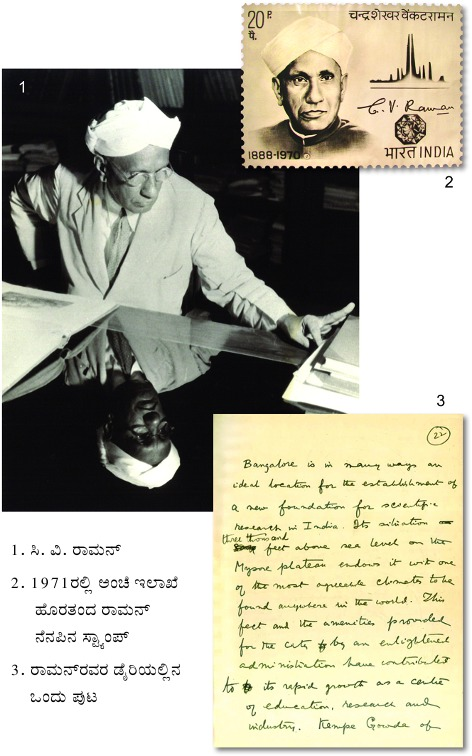
\includegraphics{images/002.jpg}
%\end{figure}


%\begin{figure}
%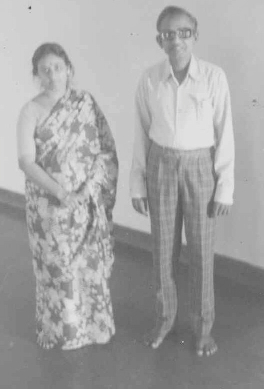
\includegraphics{images/003.jpg}
%\end{figure}


%\begin{figure}
%\includegraphics{images/004.jpg}
%\end{figure}

\footnote{1. ಪೈ ಎಂದರೆ ಪೈಸೆ (ಕಾಸು); ಹನ್ನೆರಡು ಕಾಸುಗಳು ಸೇರಿ ಒಂದು ಆಣೆ ಆಗುವುದು ಮತ್ತು ಹದಿನಾರು ಆಣೆಗಳು ಸೇರಿದರೆ ಒಂದು ರೂಪಾಯಿ ಆಗುವುದು.}

\begin{center}
\textbf{೨೧೬. ಮಿಸ್ ಜೋಸಫಿನ್ ಮ್ಯಾಕ್ಲಿಯಾಡ್ ಗೆ}
\end{center}

\begin{flushright}
ಗೋಪಾಲ್ ಲಾಲ್‌ವಿಲ್ಲ\\ಬನಾರಸ್ ಕಂಟೋನ್ಮೆಂಟ್\\ಫೆಬ್ರವರಿ ೧೪, ೧೯೦೨
\end{flushright}

ಪ್ರಿಯ ಜೊ,

ನಿನ್ನೆ ಮಿ. ಒಕಾಕುರ (ಕಾಕುಜೊ)ನಿಂದ ಒಂದು ಪತ್ರ ಬಂದಿತು. ಅವರು ಗ್ವಾಲಿ ಯರ್ಗೆ ಹೋಗುವ ದಾರಿಯಲ್ಲಿ ಆಗ್ರಾ ನೋಡಿದರು. ಈಗ ಅವರು ಅಲ್ಲಿ ಇರಬೇಕು.

ಅವರು ಜಪಾನಿಗೆ ಕಳುಹಿಸಿದ ತಂತಿ, ಮಿ. (ಟೊಕುನೊ) ಓಡ ಅವರಿಗೆ –ಕೂಡಲೆ ಬರುವಂತೆ. ಅಲ್ಲಿ ಒಂದು ಕೆಲಸವಿತ್ತು. ಅದರಲ್ಲಿ “ಆರು” ಕೂಡ ಸೇರಿದೆ.

ಇಲ್ಲಿ ಈಗಲೂ ಕೂಡ ತಂಪಾಗಿದೆ – ಮತ್ತು ಕನಿಷ್ಠ ಪಕ್ಷ ಈ ತಿಂಗಳು ಹೀಗೆಯೇ ಇರುವುದು. ಕಲ್ಕತ್ತದಲ್ಲಿ ಬಿಸಿಲು ಏರುತ್ತಿದೆಯೇ?

ಮಿಸೆಸ್ (ಓಲ್) ಬುಲ್ ಮತ್ತು ನಿವೇದಿತಾ, ದೀರ್ಘ ಪ್ರಯಾಣದ ನಂತರ ಚೆನ್ನಾಗಿ ವಿಶ್ರಾಂತಿ ಪಡೆಯುತ್ತಿರುವರೆಂದು ಭಾವಿಸುತ್ತೇನೆ.

ನಾನು ಸಾಧಾರಣವಾಗಿ ಇದ್ದೇನೆ.

ಹುಡುಗರೆಲ್ಲರೂ ಅವರ ಪ್ರೀತಿಯನ್ನು ತಿಳಿಸುತ್ತಿರುವರು.

\begin{flushright}
ಪ್ರೀತಿ ಮತ್ತು ಆಶೀರ್ವಾದಗಳೊಂದಿಗೆ ಎಂದಿಗೂ ನಿನ್ನವ,\\ವಿವೇಕಾನಂದ
\end{flushright}

\begin{center}
\textbf{೨೧೭. ಮಿಸೆಸ್ ಅಲೀಸ್ (ಶಾಂತಿ) ಹ್ಯಾನ್ಸ್ ಬ್ರೊಗೆ}
\end{center}

\begin{flushright}
ಬನಾರಸ್\\ಫೆಬ್ರವರಿ ೧೪, ೧೯೦೨
\end{flushright}

ನನ್ನ ಪ್ರಿಯ ಮಿಸೆಸ್ ಹ್ಯಾನ್ಸ್ ಬ್ರೊ,

ನೀನು ಹಿಂದೆ ನನಗಾಗಿ ಮಾಡಿರುವುದಕ್ಕಾಗಿ ನಾನು ನಿನಗೆ ಅನಂತ ಆಭಾರಿಯಾಗಿದ್ದೇನೆ, ಮತ್ತು ಈಗ ನೀನು ತುರೀಯಾನಂದರಿಗೆ ಮಾಡುತ್ತಿರುವುದಕ್ಕೆ ಇನ್ನೂ ಹೆಚ್ಚು ಋಣಿಯಾಗಿದ್ದೇನೆ.

ಅವರ ದಾರುಣ ಖಾಯಿಲೆಯ ವಾರ್ತೆ ಕಲ್ಕತ್ತೆಯನ್ನು ತಲುಪಿದಾಗ ಮಠದಲ್ಲಿ ಮಂಕು ಕವಿಯಿತು. ಅವರು ಸಂಪೂರ್ಣ ಗುಣವಾಗಿರುವರೆಂದು ಭಾವಿಸುತ್ತೇನೆ. ನಿನ್ನಿಂದ ಸಮಾಚಾರ ಬಂದರೆ ನನಗೆ ಬಹಳ ಸಂತೋಷವಾಗುವುದು.

ಅಮೆರಿಕಾದ ಹವಾಗುಣ ಅವರಿಗೆ ಸರಿಹೋಗುವುದಿಲ್ಲವೆಂದು ತೋರುವುದು. ಹಾಗಿದ್ದಲ್ಲಿ ಅವರಿಗೆ ಬೇಕೆನಿಸಿದಾಗ, ಅವರು ಭಾರತಕ್ಕೆ ಹಿಂದಿರುಗುವುದು ಒಳ್ಳೆಯದು.

ಬಹುತೇಕ ಇನ್ನು ಒಂದೆರಡು ತಿಂಗಳಲ್ಲಿ ನಾನು ಜಪಾನಿಗೆ ಹೋಗುವೆನು. ರಾಮಕೃಷ್ಣಾನಂದ ನನ್ನೊಡನೆ ಬರುವನು. ತುರೀಯಾನಂದ ಜಪಾನಿಗೆ ಬರಬಹುದು ಮತ್ತು ನಾನು ಅಮೆರಿಕಾಕ್ಕೆ ಹೋಗುವೆನು. “ತಾಯಿಗೆ” ಚೆನ್ನಾಗಿ ಗೊತ್ತು, ನಾವು ಅವಳ ಆಣತಿಯನ್ನು ಪಾಲಿಸುವೆವು.

ಸದ್ಯದಲ್ಲಿ ನಾನೀಗ ಕೆಲವು ದಿನಗಳ ಮಟ್ಟಿಗೆ ಬನಾರಸ್ನಲ್ಲಿ ಇರುವೆನು. ಅದು ಏನೇ ಇರಲಿ, ಎಲ್ಲಾ ಪತ್ರಗಳೂ ಬೇಲೂರು ಮಠದ ವಿಳಾಸಕ್ಕೆ ಕಳುಹಿಸಲ್ಪಡಲಿ.

ತುರೀಯಾನಂದನಿಗೆ ದಯವಿಟ್ಟು ನನ್ನ ಪ್ರೀತಿಯನ್ನು ತಿಳಿಸು. ನಿನಗೆ, ನಿನ್ನ ಪವಿತ್ರ ಸಂಸಾರಕ್ಕೆ ಮತ್ತು ಇತರ ಸ್ನೇಹಿತರಿಗೆ ನನ್ನ ಪ್ರೀತಿಗಳು.

\begin{flushright}
ಭಗವಂತನಲ್ಲಿ ಎಂದಿಗೂ ನಿನ್ನವ,\\ವಿವೇಕಾನಂದ
\end{flushright}

ವಿ.ಸೂ.: ತುರೀಯಾನಂದ ಸಂಪೂರ್ಣ ವಿಶ್ರಾಂತಿ ಪಡೆಯಲಿ. ನಾನು ಜಪಾನ್ ಅಥವಾ ಅಮೆರಿಕಾ ತಲಪುವವರೆಗೆ ಅವನು ಕೆಲಸ ಮಾಡುವುದೇ ಬೇಡ.

\begin{center}
\textbf{೨೧೮. ಸೋದರಿ ನೀವೇದಿತಾಳಿಗೆ}
\end{center}

\begin{flushright}
ಗೋಪಾಲ್ ಲಾಲ್‌ವಿಲ್ಲ,\\ಬನಾರಸ್ ಕಂಟೋನ್ಮೆಂಟ್,\\ಮಾರ್ಚ್ ೦೪, ೧೯೦೨
\end{flushright}

ನನ್ನ ಪ್ರಿಯ ಮಾರ್ಗೊ (ಮಾರ್ಗಾಟ್),

ಈಗ ರಾತ್ರಿಯಾಗಿದೆ, ನನಗೆ ಎದ್ದು ಕುಳಿತುಕೊಳ್ಳುವುದಕ್ಕಾಗಲಿ ಅಥವಾ ಬರೆಯುವುದಕ್ಕಾಗಲಿ ಆಗುವುದಿಲ್ಲ. ಆದರೂ ಈ ಪತ್ರವನ್ನು ಬರೆಯುವುದು ನನ್ನ ಕರ್ತವ್ಯವೆಂಬ ದೃಷ್ಟಿಯಿಂದ ಬರೆಯುತ್ತಿದ್ದೇನೆ. ಇಲ್ಲದಿದ್ದರೆ, ಇದು ನನ್ನ ಕೊನೆಯ ಪತ್ರವಾಗಬಹುದು ಮತ್ತು ಇತರರಿಗೆ ತೊಂದರೆಯಾಗಬಹುದು.

ನನ್ನ ಸ್ಥಿತಿ ಗಂಭೀರವಾಗಿ ಏನೂ ಇಲ್ಲ, ಆದರೆ ಅದು ಯಾವ ಸಮಯದಲ್ಲಿ ಬೇಕಾದರೂ ಹಾಗಾಗಬಹುದು; ಜ್ವರ ಸ್ವಲ್ಪವೇ ಇದೆ, ಮತ್ತು ಯಾವಾಗಲೂ ಎಡೆಬಿಡದೆ ಇದೆ ಮತ್ತು ಉಸಿರಾಟ ಕಷ್ಟವಾಗಿದೆ. ಇದು ಏತಕ್ಕೆ ಹೀಗೆ ಎಂಬುದು ತಿಳಿಯುತ್ತಿಲ್ಲ.

ಈಗ ಕ್ರಿಸ್ಟಿನಾ (ಗ್ರೀನ್ ಸ್ಟೈಡಲ್)ಗೆ ಮಿಸೆಸ್ (ಚಾರ್ಲಾಟ್) ಸೇವಿಯರ್ ಅವರಿಂದ ೧೦೦ ಪೌಂಡ್ಗಳನ್ನು ಭಾರತಕ್ಕೆ ಪ್ರಯಾಣ ಮಾಡಲು ಕಳುಹಿಸಿದೆ. ಆ ಸಮಯದಲ್ಲಿ ಆಕೆಯ ತಾಯಿ ಕಾಲವಾದರು. ಅವಳ ಕಳೆದ ಪತ್ರದಲ್ಲಿ ಅವಳು ಫೆಬ್ರವರಿ ೧೫ರಂದು ಸಮುದ್ರಯಾನ ಪ್ರಾರಂಭಿಸುವುದಾಗಿ ತಿಳಿಸಿದ್ದಳು. ಹಾಗಿದ್ದಲ್ಲಿ, ಅವಳು ಭಾರತಕ್ಕೆ ಬರುವ ಸಮಯ ಹತ್ತಿರವಾಗಿದೆ. ಅವಳು ಯಾವ ಬಂದರಿಗೆ ಬರುವಳು ಮತ್ತು ಹಡಗಿನ ಹೆಸರು – ಇವುಗಳ ವಿಷಯವಾಗಿ ಮುಂದಿನ ವಾರ ಪತ್ರ ನಿರೀಕ್ಷಿಸುತ್ತಿರುವೆನು. ಒಂದು ವೇಳೆ ನಾನು ಕಾಲವಾದರೆ – ಶಿವನ ನಗರಿಯಾದ ಇಲ್ಲಿ ಪ್ರಾಣ ಬಿಡಲು ನಾನು ಬಹಳ ಇಚ್ಛಿಸುವೆನು – ನನಗೆ ಬರುವ ಅವಳ ಪತ್ರಗಳನ್ನು ಒಡೆದು ಓದಿ, ಅವಳನ್ನು ಬರಮಾಡಿಕೊಂಡು, ಅವಳನ್ನು ಹಿಂತಿರುಗಿ ಕಳುಹಿಸಿಕೊಡುವೆಯಾ? ಹಿಂತಿರುಗಲು ಅವಳಲ್ಲಿ ಹಣವಿಲ್ಲದಿದ್ದರೆ ಅವಳಿಗೆ ಹಣಕೊಡು – ಅದಕ್ಕಾಗಿ ನೀನು ಭಿಕ್ಷೆ ಬೇಡಬೇಕಾದರೂ ಸರಿ.

ನಾನು ಯೂರೋಪ್ನಿಂದ ತಂದ ಸ್ವಲ್ಪ ಹಣವನ್ನು ನನ್ನ ತಾಯಿಯನ್ನು ಕಾಪಾಡಲು ಮತ್ತು ಅವಳ ಸಾಲಗಳನ್ನು ತೀರಿಸಲು ಖರ್ಚು ಮಾಡಿದೆ. ಉಳಿದಿರುವ ಸ್ವಲ್ಪ ಹಣವನ್ನು ನಾನು ಮುಟ್ಟುವಂತಿಲ್ಲ, ಏಕೆಂದರೆ ಅದು ಕೋರ್ಟ್ನಲ್ಲಿ ಇರುವ ಕೇಸ್ ನ ವೆಚ್ಚಕ್ಕಾಗಿ.

ನಾನು ಸಾಯದೆ ಎಳೆದಾಡುತ್ತಿದ್ದರೆ, ಅವಳು ಬರುವ ಸಮಯವನ್ನು ನಿನಗೆ ತಿಳಿಸುತ್ತೇನೆ. ಆಗ ನೀನು ಅವಳು ಕ್ಷೇಮವಾಗಿ ಬರೇಲಿಯ ಒಂದು ಸ್ಟೇಷನ್ಗೆ ಕ್ಷೇಮವಾಗಿ ಬರುವಂತೆ ನೋಡಿಕೊಳ್ಳಬೇಕು. ಅಲ್ಲಿ ನಾನು ಅವಳನ್ನು ಭೇಟಿ ಮಾಡುತ್ತೇನೆ. ಅವಳು ಮಿಸೆಸ್ (ಚಾರ್ಲಾಟ್) ಸೇವಿಯರ್ ಅವರ ಅತಿಥಿಯಾಗಿರಬೇಕು. ನಾನೂ ಕೂಡ ಆಲ್ಮೋರಕ್ಕೆ ಮತ್ತೊಮ್ಮೆ ಹೋಗಲು ಯತ್ನಿಸುತ್ತೇನೆ.

ನಾನು ಹೊರಟು ಬರುವುದಕ್ಕೆ ಕೆಲವು ವಾರಗಳ ಮೊದಲು ರಾಮಕೃಷ್ಣಾನಂದ ಬಂದನು. ಆತ ಮಾಡಿದ ಮೊದಲ ಕೆಲಸವೆಂದರೆ ನನ್ನ ಕಾಲಿನ ಬಳಿ ತಾನು ಹಲವು ವರ್ಷಗಳು ಕಷ್ಟಪಟ್ಟು ಸಂಗ್ರಹಿಸಿದ್ದ ರೂ. ೪೦೦ನ್ನು ಇಟ್ಟನು. ಅಂತಹ ಘಟನೆ ನನ್ನ ಜೀವನದಲ್ಲಿ ನಡೆದುದು ಅದೇ ಮೊದಲು. ನನ್ನ ಕಣ್ಣೀರನ್ನು ತಡೆದುಕೊಳ್ಳಲಾಗುತ್ತಿಲ್ಲ. ಓ, ತಾಯಿ! ತಾಯಿ! ಎಲ್ಲ ಕೃತಜ್ಞತೆ, ಎಲ್ಲ ಪ್ರೀತಿ, ಎಲ್ಲ ಪೌರುಷ ಇನ್ನೂ ಸತ್ತಿಲ್ಲ!!! ಪ್ರೀತಿಯ ಮಗು, ಒಂದು ಸಾಕು – ಪ್ರಪಂಚದಲ್ಲಿ ಕಾಡನ್ನು ಬೆಳೆಸಲು ಒಂದು ಬೀಜ ಸಾಕು.

ಒಳ್ಳೆಯದು, ಆ ಹಣ ಬೇಲೂರು ಮಠದಲ್ಲಿ ನಿಧಿಯಾಗಿ ಇಡಲ್ಪಟ್ಟಿದೆ. ಅದರ ಒಂದು ಕಾಸನ್ನೂ ನಾನು ಮುಟ್ಟುವುದಿಲ್ಲ. ಆ ಹಣವನ್ನು ತನ್ನವರಿಗೆ ಕೊಡುವಂತೆ ನಾನು ರಾಮಕೃಷ್ಣಾನಂದನಿಗೆ ಹೇಳಿದಾಗ, ಅವನು ಅದಕ್ಕೆ ಸ್ವಲ್ಪವೂ ಇಚ್ಛೆ ಪಡುವುದಿಲ್ಲವೆಂದೂ ಮತ್ತು ನನಗೆ ಮಾತ್ರವೇ ಕೊಡುವುದಾಗಿ ಹೇಳಿದನು. ಅಲ್ಲದೆ, ತಾನು ಅಷ್ಟು ಅಲ್ಪ ಹಣವನ್ನು ಮಾತ್ರ ನಾಲ್ಕು ವರ್ಷಗಳಲ್ಲಿ ಸೇರಿಸಲು ಸಾಧ್ಯವಾದುದಕ್ಕೆ ಪರಿತಾಪ ಪಟ್ಟನು! ನಾನು ಕಾಲವಾದರೆ, ಆ ೪೦೦ ರೂಪಾಯಿಗಳು – ಒಂದು ರೂಪಾಯಿಯೂ ಬಿಡದಂತೆ – ಅವನಿಗೆ ತಲುಪುವಂತೆ ನೋಡಿಕೊ. ಭಗವಂತನು ನಿನ್ನನ್ನೂ ರಾಮಕೃಷ್ಣಾನಂದನನ್ನೂ ಹರಸಲಿ.

ನನ್ನ ಕೆಲಸದ ಬಗ್ಗೆ ನಾನು ಪೂರ್ಣ ತೃಪ್ತನಾಗಿರುವೆ. ಇಬ್ಬರು ನಿಜವಾದ ಪರಿಶುದ್ಧಾತ್ಮ ರನ್ನು ಹಿಂದೆ ಬಿಟ್ಟು ಹೋಗುವುದು ಅತ್ಯಂತ ದೊಡ್ಡ ವ್ಯಕ್ತಿಗಳ ಹಂಬಲವನ್ನೂ ಮೀರಿದುದು.

\begin{flushright}
ಎಂದಿಗೂ ನಿನ್ನ ಪ್ರೀತಿಯ ತಂದೆ,\\ವಿವೇಕಾನಂದ
\end{flushright}

\begin{center}
\textbf{೨೧೯. ಸೋದರಿ ಕ್ರಿಸ್ಟೈನ್ಗೆ}
\end{center}

\begin{flushright}
ಬೇಲೂರು ಮಠ,\\ಹೌರಾ ಜಿಲ್ಲೆ, ಬಂಗಾಲ\\ಮಾರ್ಚ್ ೩೦, ೧೯೦೨
\end{flushright}

ನನ್ನ ಪ್ರಿಯ ಕ್ರಿಸ್ಟೈನ್,

ನೀನು ಅದೆಷ್ಟು ಸ್ವಾಗತಾರ್ಹಳೆಂಬುದು ನಿನಗೆ ಗೊತ್ತಿದೆ – ನಾನು ಅದನ್ನು ವ್ಯಕ್ತಪಡಿಸಬೇಕಾಗಿಲ್ಲ. ಅಭಿವ್ಯಕ್ತಿಯನ್ನು ಎಚ್ಚರಿಕೆಯಿಂದ ಮಂದಗೊಳಿಸುವ ದೇಶವಿದು. ಮಾರ್ಗಾಟ್ (ಸೋದರಿ ನಿವೇದಿತಾ) ಮತ್ತು ಜೊ (ಮಿಸ್ ಜೋಸಫಿನ್ ಮ್ಯಾಕ್ಲಿಯಾಡ್) ಆಗಲೆ ಬರೆದಿರುವರು ಮತ್ತು ಬೊಂಬಾಯಿಯಲ್ಲಿ ವ್ಯವಸ್ಥೆ ಮಾಡಿರುವರು. ನಾನು ನಿನ್ನ ನಿರೀಕ್ಷೆ ಮತ್ತು ಭೇಟಿಯನ್ನು ಇಲ್ಲಿ ಕಲ್ಕತ್ತದಲ್ಲಿ ಮಾಡುವೆನು. ನಿನ್ನನ್ನು ಸ್ವಾಗತಿಸಲು ನಾನು ಬೊಂಬಾಯಿಯಲ್ಲಿ ಇದ್ದಿದ್ದರೆ ಎಷ್ಟು ಚೆನ್ನಾಗಿತ್ತೆಂದು ಭಾವಿಸುವೆನು, ಆದರೆ ನಮ್ಮ ಇಚ್ಛೆಗಳೆಲ್ಲವೂ ಪೂರ್ಣವಾಗಬೇಕಾದುದಿಲ್ಲ.

ನೇರವಾಗಿ ಬಾ; ಆದರೆ ಬಿಸಿಲಿನ ತಾಪದಿಂದ ನಿನ್ನ ತಲೆಯ ಹಿಂಭಾಗವನ್ನು ಬಹಳ ಎಚ್ಚರಿಕೆಯಿಂದ ರಕ್ಷಿಸಿಕೊ.

ಇಲ್ಲಿ ರೈಲುಗಳು ನಿಮ್ಮ ದೇಶದಂತೆ ಸುರಕ್ಷಿತವಲ್ಲ, ಆದುದರಿಂದ ರಾತ್ರಿ ಪ್ರಯಾಣ ಕಾಲದಲ್ಲಿ ನಿನ್ನ ಸಾಮಾನುಗಳ ಬಗ್ಗೆ ಎಚ್ಚರಿಕೆಯಿಂದಿರು.

ನಿನಗೆ ಆಯಾಸವಾಗಿದ್ದಲ್ಲಿ, ಬಾಂಬೆಯಲ್ಲಿ ವಿಶ್ರಾಂತಿ ತೆಗೆದುಕೊ. ಮಿಸೆಸ್ (ಓಲ್) ಬುಲ್, ಜೊ ಮತ್ತು ಮಾರ್ಗಾಟ್ ಕುತೂಹಲದಿಂದ ನಿನ್ನ ಆಗಮನವನ್ನು ನಿರೀಕ್ಷಿಸುತ್ತಿರುವರು. ಮತ್ತು ಅಂತೆಯೇ,

\begin{flushright}
ವಿವೇಕಾನಂದ
\end{flushright}

\begin{center}
\textbf{೨೨೦. ಮಿಸೆಸ್ ಓಲ್ ಬುಲ್ ಅವರಿಗೆ}
\end{center}

\begin{flushright}
ಬೇಲೂರು ಮಠ,\\ಪೋಸ್ಟ್ ಬೇಲೂರು, ಹೌರಾ\\ಮಾರ್ಚ್ (?), ೧೯೦೨
\end{flushright}

ಪ್ರಿಯ ಮಾತೆ\footnote{1. ಈ ಪತ್ರವನ್ನು ಬರೆದ ಕಾಲದಲ್ಲಿ ಮಿಸೆಸ್ ಓಲ್ ಬುಲ್ ಅವರು, ಸೋದರಿ ನಿವೇದಿತಾ, ಮಿ. ಒಕಾಕುರ ಕಾಕುಜೊ ಮತ್ತು ಮಿಸ್ ಜೋಸಫಿನ್ ಮ್ಯಾಕ್ಲಿಯಾಡ್ ಅವರೊಂದಿಗೆ ಕಲ್ಕತ್ತದಲ್ಲಿ ಅಮೆರಿಕನ್ ರಾಯಭಾರಿ ಕಛೇರಿಯಲ್ಲಿ ವಾಸವಿದ್ದರು. ಮಿಸಸ್ ಬುಲ್, ಸೋದರಿ ನಿವೇದಿತಾ ಸಂಗಡ ಫೆಬ್ರವರಿ ಎರಡನೇ ವಾರದಲ್ಲಿ ಭಾರತಕ್ಕೆ ಬಂದಿದ್ದರು ಮತ್ತು ಏಪ್ರಿಲ್ ೧೭, ೧೯೦೨ರಂದು ಕಲ್ಕತ್ತೆಯನ್ನು ಬಿಟ್ಟರು.},

ಚಿನ್ನು ಬಂದದ್ದು ನನಗೆ ಸಂತೋಷ. ನಾಳೆ ನೀವು ಬರುವುದಕ್ಕೆ ಯಾವ ಸಮಯವಾದರೂ ನನಗೆ ಸರಿಯೇ. ಆದರೆ ಇಲ್ಲಿ ಬೆಳಗ್ಗೆ ೧೧ರಿಂದ ಸಂಜೆ ೫ರವರೆಗೆ ಭಯಂಕರ ಬಿಸಿಲಿನ ತಾಪವಿರುವುದು.

ಆದುದರಿಂದ, ನೀವು ಬೆಳಗಿನ ತಿಂಡಿ ಮುಗಿದ ಮೇಲೆ ಹೊರಟು ಇಡೀ ದಿನ ಇಲ್ಲಿರಿ ಮತ್ತು ಮಧ್ಯಾಹ್ನ ಬಂಗಾಳಿ ಮೀನಿನ ಊಟ ಮಾಡಿ ಸಂಜೆ ಹಿಂತಿರುಗಿ ಎಂದು ನನ್ನ ಸಲಹೆ.

ನೀವು ಬರುವುದಕ್ಕೆ ಮತ್ತು ಹಿಂತಿರುಗುವುದಕ್ಕೆ ಒಂದು ಗಾಡಿಯನ್ನು ಗೊತ್ತು ಮಾಡಿಕೊಳ್ಳಿ ಎಂದು ನಾನು ಒತ್ತಾಯಪೂರ್ವಕವಾಗಿ ಹೇಳುತ್ತೇನೆ. ಗಾಡಿ ಬಂದು ಹೋಗುವುದಕ್ಕೆ ದೋಣಿಯಷ್ಟೆ ಅಥವಾ ಕಡಿಮೆ ಬಾಡಿಗೆ ಆಗಬಹುದು ಮತ್ತು ಸಾಗಣೆಯಲ್ಲಿ ಬದಲಾವಣೆ ಇಲ್ಲ. ಗಾಡಿಯವನಿಗೆ ಬೇಲೂರು ಗೊತ್ತಾಗದಿದ್ದರೆ, ಬಾಲಿಯಿಂದ ದಕ್ಷಿಣಕ್ಕೆ ಎರಡು ಮೈಲಿ ಹೋಗಲು ಹೇಳಿ. ಅವನಿಗೆ ಬಾಲಿ ಗೊತ್ತೇ ಇರುತ್ತದೆ ಮತ್ತು ಅಲ್ಲಿಂದ ಅವನು ಮಠಕ್ಕೆ ದಾರಿ ಕೇಳಿಕೊಂಡು ಬರಲಿ.

ಒಂದು ದಿನ ಮಿ. ಒಕಾಕುರ (ಕಾಕುಜೊ) ಅವರಿಗಾದ ನೀರಿನಲ್ಲಿ ನೆನೆದು ಮುಳುಗಿ ಹೋದ ಅನುಭವವಾದುದನ್ನು ಕೇಳಿದರೆ ಅನೇಕ ದಿನ ನೀವು ಭಯದಿಂದ ಕಂಗಾಲಾಗುವಿರಿ; ಈ ತಿಂಗಳು ಪ್ರತಿ ನಿತ್ಯ ಸಂಜೆ ನಾವು ಅಂತಹ ಭಯಂಕರ ವಾತಾವರಣವನ್ನು ನಿರೀಕ್ಷಿಸುವೆವು. ನೀವು ಇರುವ ಸ್ಥಳದಿಂದ ರಸ್ತೆಯಲ್ಲಿ ಬರುವುದು ಹತ್ತಿರ, ಸುಲಭ ಮತ್ತು ಅಗ್ಗ. ಈ ಪತ್ರವನ್ನು ತರುತ್ತಿರುವ ನಿಮ್ಮ ಸೇವಕನಿಗೂ ಸೂಚನೆಗಳನ್ನು ಕೊಟ್ಟಿರುವೆನು.

\begin{flushright}
ಎಂದಿಗೂ ನಿನ್ನ ಮಗ,\\ವಿವೇಕಾನಂದ
\end{flushright}

\begin{center}
\textbf{೨೨೧. ಮಿಸ್ ಜೋಸೆಫಿನ್ ಮ್ಯಾಕ್ಲಿಯಾಡ್ ಗೆ}
\end{center}

\begin{flushright}
ಬೇಲೂರು ಮಠ,\\ಏಪ್ರಿಲ್ ೦೨, ೧೯೦೨
\end{flushright}

ನನ್ನ ಪ್ರಿಯ ಜೋ,

ಟೆಲಿಗ್ರಾಂ ಆಗಲೇ ಹೋಗಿದೆ ಮತ್ತು ನೀನು ಅಲ್ಲಿ ಎಲ್ಲಾ ವ್ಯವಸ್ಥೆಗಳನ್ನೂ ಮಾಡುವೆ ಎಂದು ಭಾವಿಸುತ್ತೇನೆ.

ಮಾಯಾವತಿಗೆ ಹೋಗುವ ದಾರಿಯಲ್ಲಿ ಇರುವ ಡಾಕ್ ಬಂಗಲೆಯಲ್ಲಿ ಆಹಾರ ಕೊಡುವುದಿಲ್ಲ, ಅಡಿಗೆ ಮಾಡುವವರೂ ಇಲ್ಲ.

ಆಹಾರ ಸಾಮಗ್ರಿಗಳನ್ನು ಕಥಗೋಡಂನಲ್ಲಿ ಕೊಳ್ಳಬೇಕಾಗುತ್ತದೆ ಮತ್ತು ವ್ಯವಸ್ಥೆಗಳನ್ನು ಮಾಡಿಕೊಳ್ಳಬೇಕಾಗುತ್ತದೆ.

ನಿಮಗೇನಾದರೂ ತೊಂದರೆಯಾದಲ್ಲಿ, ನೇರ ಆಲ್ಮೋರಾಕ್ಕೆ ಹೋಗಿ ಮತ್ತು ಅಲ್ಲಿ ಸಾವಕಾಶವಾಗಿ ವ್ಯವಸ್ಥೆ ಮಾಡಿಕೊಳ್ಳಿ. ಆಲ್ಮೋರಾಕ್ಕೆ ಹೋಗುವ ದಾರಿಯಲ್ಲಿ ಸಿಕ್ಕುವ ಡಾಕ್ ಬಂಗಲೆಗಳಲ್ಲಿ ಆಹಾರ ದೊರೆಯುವುದು ಮತ್ತು ಆಲ್ಮೋರಾದಲ್ಲಿ ಒಂದು ಒಳ್ಳೆಯ ಡಾಕ್ ಬಂಗಲೆ ಇದೆ.

ಎಂದಿನಂತೆ ಎಲ್ಲವೂ ನಿಮಗೆ ಅನುಕೂಲವಾಗುತ್ತವೆ ಎಂದು ಭಾವಿಸುತ್ತೇನೆ– ತಾತನ\footnote{1. ಇಲ್ಲಿ ‘ತಾತ’ ಎಂದರೆ ಸ್ವಾಮಿ ವಿವೇಕಾನಂದರೆ.} ಆರೋಗ್ಯ ಹೊರತು.

\begin{flushright}
ವಿಶ್ವಾಸಪೂರ್ವಕವಾಗಿ ನಿನ್ನವ,\\ವಿವೇಕಾನಂದ
\end{flushright}

ನನಗೆ ಮಿ. (ಟೊಕುನೊ) ಒಡ ಬಹಳ ಇಷ್ಟವಾದರು – ಅವರಿಗೆ ತಮ್ಮ ಕೆಲಸದಲ್ಲಿ ಆಸಕ್ತಿ ಇದೆ.

\begin{flushright}
ವಿವೇಕಾನಂದ
\end{flushright}

\begin{center}
\textbf{೨೨೨. ಸೋದರಿ ಕ್ರಿಸ್ಟೈನ್ಗೆ}
\end{center}

\begin{flushright}
ಬೇಲೂರು ಮಠ, ಹೌರಾ ಜಿಲ್ಲೆ\\ಮೇ ೧೫, ೧೯೦೨
\end{flushright}

ನನ್ನ ಪ್ರಿಯ ಕ್ರಿಸ್ಟೈನ್,

ನಿನಗೆ ಮಾಯಾವತಿ ಇಷ್ಟವಾಯಿತೆಂದು ತಿಳಿದು ಸಂತೋಷವಾಯಿತು. ಇಲ್ಲಿ ಉಷ್ಣ ಜೋರಾಗಿದೆ, ಮತ್ತು ಮಳೆ ಇಲ್ಲ. ಆದರೂ ನಾನು ಬಹಳ ಕಡಿಮೆ ನೀರು ಕುಡಿಯುತ್ತೇನೆ.

ನಾನು ಮಾಯಾವತಿ ಅಥವಾ ಆಲ್ಮೋರಾಕ್ಕೆ ಹೋಗುವ ಆಲೋಚನೆಯನ್ನು ಸಂಪೂರ್ಣವಾಗಿ ಕೈಬಿಟ್ಟಿದ್ದೇನೆ. ಧಗೆಯನ್ನು ಸಹಿಸುತ್ತೇನೆ, ಆದರೆ ಇಲ್ಲಿನ ಮಳೆಯಿಂದ ಪಾರಾಗಬೇಕು. ಮಳೆ ಬಂದಾಗ ನಾನು ಮತ್ತೆಲ್ಲಿಗಾದರೂ ಹೋಗುತ್ತೇನೆ.

ಕಲ್ಕತ್ತೆಯಿಂದ ಸಮಾಚಾರವಿಲ್ಲ. ನಾನು ಅವಸರದಲ್ಲಿದ್ದೇನೆ. ನೀನು ಅಲ್ಲಿ ಏನನ್ನು ನೋಡುವೆಯೊ ಅಥವಾ ಏನು ಭಾವಿಸುವೆಯೊ – ವ್ಯಕ್ತಿಗಳ ಮತ್ತು ವಸ್ತುಗಳ ಬಗ್ಗೆ – ಅದರ ವಿವರವನ್ನು ಬರೆ.

\begin{flushright}
ಎಲ್ಲ ಪ್ರೀತಿಗಳೊಂದಿಗೆ ನಿನ್ನವ,\\ವಿವೇಕಾನಂದ
\end{flushright}

\begin{center}
\textbf{೨೨೩. ಮೇಡಂ ಎಮ್ಮಾ ಕಾಲ್ವೆಯವರಿಗೆ}
\end{center}

(ಮೇಡಂ ಕಾಲ್ವೆಯವರ ತಂದೆ ಕಾಲವಾದ ಸಂದರ್ಭದಲ್ಲಿ ಈ ಅನುತಾಪದ ಪತ್ರವನ್ನು ಬರೆಯಲಾಗಿತ್ತು ಮತ್ತು ಮಿಸ್ ಜೋಸೆಫಿನ್ ಮ್ಯಾಕ್ಲಿಯಾಡ್ ಅವರಿಗೆ ಬರೆದ ಪತ್ರದೊಡನೆ ಅದನ್ನು ಇಡಲಾಗಿತ್ತು.)

\begin{flushright}
ಬೇಲೂರು ಮಠ, ಹೌರಾ ಜಿಲ್ಲೆ, ಬಂಗಾಳ, ಭಾರತ\\ಮೇ ೧೫, ೧೯೦೨
\end{flushright}

ನನ್ನ ಪ್ರಿಯ ಮೇಡಂ,

ನಿಮ್ಮ ಮೇಲೆ ಎರಗಿದ ದುಃಖಪೂರಿತ ವಿಯೋಗವನ್ನು ತಿಳಿದು ಬಹಳ ವ್ಯಸನವಾಯಿತು.

ಈ ಆಘಾತಗಳು ನಮ್ಮೆಲ್ಲರ ಮೇಲೆ ಆಗಬೇಕು. ಅವು ಸಹಜವಾಗಿ ಆಗುವುದು, ಆದರೂ ಅವನ್ನು ಸಹಿಸುವುದು ಬಹಳ ಕಷ್ಟ.

ಒಡನಾಟದ ಶಕ್ತಿ ಅಸತ್ಯವಾದ ಈ ಪ್ರಪಂಚವನ್ನು ಸತ್ಯವೆನಿಸುವಂತೆ ಮಾಡುವುದು, ಒಡನಾಟ ದೀರ್ಘವಾದಷ್ಟು, ನೆರಳು ಹೆಚ್ಚು ಸತ್ಯದಂತೆ ಕಾಣುವುದು. ಆದರೆ, ಅಸತ್ಯ ಅಸತ್ಯ ದೆಡೆಗೆ ಹೋಗುವ ದಿನ ಬರುವುದು; ಹಾ! ಅದು ಸಹಿಸಲು ಎಷ್ಟು ಕಷ್ಟ.

ಆದರೂ, ಯಾವುದು ಸತ್ಯವೊ, ಎಲ್ಲೆಡೆ ಇರುವುದೊ, ಆ ಆತ್ಮ, ಸದಾ ನಮ್ಮೊಡ ನಿರುವುದು. ಯಾರು, ಮಾಯವಾಗುವ ನೆರಳಿನ ಪ್ರಪಂಚದಲ್ಲಿ ಸತ್ಯವನ್ನು ಕಂಡಿರುವನೊ ಅವನು ಧನ್ಯ.

ಪ್ರಿಯ ಮೇಡಂ, ಕಳೆದ ಬಾರಿ ನಾವು ಈಜಿಪ್ಟ್ನಲ್ಲಿ ಭೇಟಿಯಾದ ನಂತರ ನಿಮ್ಮ ಆರೋಗ್ಯ ಬಹಳಷ್ಟು ಉತ್ತಮವಾಗಿರುವುದು ಎಂದು ನಾನು ಭಾವಿಸುತ್ತೇನೆ.

ಭಗವಂತನು ಅವನ ಶ್ರೇಷ್ಠ ಆಶೀರ್ವಾದಗಳನ್ನು ಯಾವಾಗಲೂ ನಿಮ್ಮ ಮೇಲೆ ವರ್ಷಿಸಲಿ ಎಂದು ಸದಾ ಪ್ರಾರ್ಥಿಸುವ,

\begin{flushright}
ವಿವೇಕಾನಂದ
\end{flushright}

\begin{center}
\textbf{೨೨೪. ಸೋದರಿ ಕ್ರಿಸ್ಟೈನ್ಗೆ}
\end{center}

\begin{flushright}
ಬೇಲೂರು ಮಠ, ಹೌರಾ ಜಿಲ್ಲೆ\\ಮೇ ೨೭, ೧೯೦೨
\end{flushright}

ನನ್ನ ಪ್ರಿಯ ಕ್ರಿಸ್ಟೈನ್,

ಈ ಬಾರಿ ನಾನು ಪರ್ವತಗಳಿಗೆ ಬರಲಾಗದಿದ್ದುದಕ್ಕೆ ವಿಷಾದಿಸುತ್ತೇನೆ. ನನ್ನ ಆರೋಗ್ಯ, ನಾನು ಇಚ್ಛಿಸಿದಷ್ಟು ಉತ್ತಮಗೊಳ್ಳದಿದ್ದರೂ, ಕೆಟ್ಟದ್ದಾಗಿಲ್ಲ. ಪಿತ್ತ ಕೋಶಕ್ಕೆ ಪ್ರಯೋಜನವಾಗಿದೆ – ಅದೊಂದು ದೊಡ್ಡ ಲಾಭ. ಬೆಟ್ಟ ಪ್ರದೇಶಗಳಲ್ಲಿ ಮಳೆ ಇನ್ನೇನು ಪ್ರಾರಂಭವಾಗಲಿದೆ. ಆದುದರಿಂದ ಆ ಭಯಂಕರ ಮಾರ್ಗದಲ್ಲಿ ಬರಲು ತೊಂದರೆ ತೆಗೆದುಕೊಳ್ಳುವುದು ಅಪ್ರಯೋಜಕ.

ಪರ್ವತ ಪ್ರದೇಶ ನಿನಗೆ ಒಳ್ಳೆಯದು ಮಾಡುತ್ತಿದೆ ಎಂದು ತಿಳಿಯಲು ನನಗೆ ಬಹಳ ಸಂತೋಷವಾಗುತ್ತಿದೆ. ಚೆನ್ನಾಗಿ ಊಟ ಮಾಡು, ಸಾಧ್ಯವಾದಷ್ಟು ಹೆಚ್ಚಾಗಿ ನಿದ್ರಿಸು, ಮತ್ತು ದಪ್ಪವಾಗು. ದಪ್ಪವಾಗುವವರೆಗೂ ಚೆನ್ನಾಗಿ ತಿನ್ನು ಇಲ್ಲವೇ ಒಡೆದು ಹೋಗು.

ಹಾಗಾದರೆ, ಆ ಸ್ಥಳ ಒಕಾಕುರ (ಕಾಕುಜೊ) ಅವರಿಗೆ ಸರಿಹೋಗಲಿಲ್ಲ – ಏಕೆ? ಅವರಿಗೆ ತುಂಬ ಬೇಜಾರಾಗುವಂತಹುದೇನೊ ನಡೆದಿರಬೇಕು, ಅದಕ್ಕೇ ಅವರು ಇದ್ದ ಕ್ಕಿದ್ದಂತೆ ಸ್ಥಳ ಬಿಟ್ಟುಹೋದರು. ಅವರಿಗೆ ಅಲ್ಲಿನ ದೃಶ್ಯ ಇಷ್ಟವಾಗಲಿಲ್ಲವೇ? ಅದರ ಔನ್ನತ್ಯ ಅವರಿಗೆ ಸಾಲದಾಯಿತೇ? ಅಥವಾ ಜಪಾನಿಯರಿಗೆ ಔನ್ನತ್ಯವೇ ಇಷ್ಟವಾಗುವುದಿಲ್ಲವೋ? ಅವರು ಕೇವಲ ಸೌಂದರ್ಯವನ್ನು ಇಷ್ಟ ಪಡುವರು.

ಚಿಕ್ಕ ಹುಡುಗ ಅವಿಧೇಯನಾಗುತ್ತಿರುವನು ಎಂದು ಹುಡುಗರಲ್ಲೊಬ್ಬ ಬರೆ ಯುತ್ತಾನೆ. ಆ ಹುಡುಗನನ್ನು ನಾನು ಅಲ್ಲಿಂದ ಕರೆಸಬೇಕೆಂದು ಮಿಸೆಸ್ ಸೇವಿಯರ್ ಇಚ್ಛಿಸುವರು. ನಾನು ಹಾಗೆಯೇ ಮಾಡುತ್ತೇನೆ. ಸದಾನಂದ ಮತ್ತು ಇನ್ನೊಬ್ಬ ಸಂನ್ಯಾಸಿ (ಆತ ಇಲ್ಲಿ ಕೆಲಸ ಮಾಡಲು ಬೇಕಾಗಿದೆ)ಯನ್ನು ಆಲ್ಮೋರಕ್ಕೆ ಹೋಗಿ, ಮಳೆ ಪ್ರಾರಂಭವಾಗುವವರೆಗೆ ಅಲ್ಲಿದ್ದು, ನಂತರ ಇಲ್ಲಿಗೆ ಬರಲು ನಾನು ಹೇಳಿದ್ದೇನೆ.

ಮಿಸೆಸ್ ಸೇವಿಯರ್ ಅವರಿಗೆ ನಿನ್ನಿಂದ ಅತ್ಯಲ್ಪ ಹೊರೆ ಎಂದೆನಿಸಿದರೂ ನೀನು ನನಗೆ ಕೂಡಲೆ ಬರೆ. ಅವರ ಮೇಲೆ ಇನ್ನೂ ಒತ್ತಡ ಹೇರುವುದು ಒಂದು ಪಾಪ – ಅವರು ನನಗಾಗಿ ಎಷ್ಟೊಂದನ್ನು ಮಾಡುವರು. ಅದೇನೇ ಆದರೂ, ಅವರು ನಿನ್ನನ್ನು ಬಹಳ ಇಷ್ಟಪಡುವರು ಮತ್ತು ನೀನು ಸೀರೆ ಉಟ್ಟರೆ ತುಂಬಾ ಸುಂ – ದ – ರ –ವಾಗಿ ಕಾಣುವೆಯೆಂದು ನನಗೆ ಬರೆಯುವರು.

ನನ್ನ ಸಂಸಾರಕ್ಕೆ ಎರಡು ಆಡಿನ ಮರಿಗಳು ಮತ್ತು ಮೂರು ಕುರಿಮರಿಗಳು ಸೇರಿವೆ. ಇನ್ನೂ ಒಂದು ಆಡಿನ ಮರಿ ಇತ್ತು, ಆದರೆ ಅದು ಹಳದಿ ಮೀನಿನ ಕೆರೆಯಲ್ಲಿ ಮುಳುಗಿ ಸತ್ತು ಹೋಯಿತು. ಮಾರ್ಗಾಟ್ ಹೇಗಿರುವಳು? ಅವಳು ಇನ್ನೂ ಅಲ್ಲಿರುವಳೇ ಅಥವಾ ಮಿ. ಒಕಾಕುರ ಅವರೊಂದಿಗೆ ಹೋದಳೇ? ಹುಡುಗರೊಂದಿಗೆ ಅವಳು ಹೇಗೆ ನಿಭಾಯಿಸುತ್ತಿರುವಳು?

ಇಡಿ ದಿನ ನೀನು ಏನು ಮಾಡುವೆ? ದಿನವನ್ನು ಹೇಗೆ ಕಳೆಯುವೆ? ಎಲ್ಲ ವಿವರಗಳನ್ನೂ ಬರೆ, ಆಗಾಗ್ಗೆ ಬರೆ; ಆದರೆ ನನ್ನಿಂದ ದೀರ್ಘವಾದ ಮತ್ತು ಬೇಗ ಬೇಗ ಪತ್ರಗಳನ್ನು ನಿರೀಕ್ಷಿಸ ಬೇಡ.

ನನ್ನ ಪ್ರೀತಿಯನ್ನು ಮಿಸೆಸ್ ಸೇವಿಯರ್, ಮಾರ್ಗಾಟ್ ಮತ್ತು ಉಳಿದವರಿಗೆ ಕೊಡು, ಮತ್ತು ಇಚ್ಛಿಸುವುದಾದರೆ, ನೀನು ಒಂದೆರಡು ಚಮಚಗಳಷ್ಟು ತೆಗೆದುಕೊಳ್ಳಬಹುದು.

\begin{flushright}
ಇಷ್ಟು ಮಾತ್ರ,\\ವಿವೇಕಾನಂದ
\end{flushright}

ವಿ.ಸೂ.: ಸಣ್ಣವನ ಮೇಲೆ ನಿಗಾ ಇರಲಿ. ಹುಡುಗರು ಆಗಲೆ ಅವನ ಬಗ್ಗೆ ಅಸೂಯೆಯಿಂದಿರುವರು. ಅವರು ಮತ್ತೊಬ್ಬ ಹುಡುಗನನ್ನು ಅದೇ ರೀತಿ ಹಾಳು ಮಾಡಿದರು.

\begin{flushright}
ವಿ.
\end{flushright}

\begin{center}
\textbf{೨೨೫. ಸೋದರಿ ಕ್ರಿಸ್ಟೈನ್ಗೆ}
\end{center}

\begin{flushright}
ಬೇಲೂರು ಮಠ, ಹೌರಾ ಜಿಲ್ಲೆ\\ಜೂನ್ ೧೪, ೧೯೦೨
\end{flushright}

ನನ್ನ ಪ್ರಿಯ ಕ್ರಿಸ್ಟೈನ್,

ನಿನ್ನ ಪತ್ರಗಳು ಕೆಲವು ದಿನಗಳು ಕಾಯಬೇಕಾಯಿತು, ಏಕೆಂದರೆ ನಾನು ಊರಿನಿಂದ ಹೊರಗೆ ಒಂದು ಹಳ್ಳಿಗೆ\footnote{1. ಸ್ವಾಮಿ ಬ್ರಹ್ಮಾನಂದರ ದಿನಚರಿಯ ಪ್ರಕಾರ ಸ್ವಾಮಿ ವಿವೇಕಾನಂದರು ಬೊರೊ ಜಗುಲಿಯಾಕ್ಕೆ ಜೂನ್ ೬ರಂದು ಹೋದರು. ಅವರು ಮೊದಲು ರೈಲಿನಲ್ಲಿ ಸಿಯಾಲ್ಡಾದಿಂದ ಸುಮಾರು ಮೂವತ್ತು ನಾಲ್ಕು ಕಿ.ಮೀ. ದೂರವಿರುವ ಕಾಂಚ್ರಾಪಾರಕ್ಕೆ ಪ್ರಯಾಣ ಮಾಡಿದರು. ಅಲ್ಲಿಂದ ಸ್ವಾಮೀಜಿ ಸುಮಾರು ಏಳು ಮೈಲಿಗಳು ಎತ್ತಿನ ಗಾಡಿಯಲ್ಲಿ, ಅವರ ಶಿಷ್ಯೆಯಾದ ಶ‍್ರೀಮತಿ ಮೃಣಾಲಿನಿ ಬಸು ಅವರ ಬೇಡಿಕೆಯಂತೆ, ಅವರ ವಾಸ ಸ್ಥಳವಾದ ಬೊರೊ ಜಗುಲಿಯಾ ಹಳ್ಳಿಗೆ ಹೋದರು.} ಹೋಗಿದ್ದೆ. ನನಗೆ ಅನೇಕ ವಿಷಯಗಳನ್ನು ತಿಳಿಸಿದುದಕ್ಕೆ ಅನೇಕ ಧನ್ಯವಾದಗಳು. ಮಿ. ಓಕಾಕುರ (ಕಾಕುಜೊ) ಮಠಕ್ಕೆ ಬಂದಿದ್ದರು, ಆದರೆ ನಾನು ಹೊರಗೆ ಹೋಗಿದ್ದೆ. ಅವರು ಇನ್ನು ಕೆಲವು ವಾರ ಕಲ್ಕತ್ತದಲ್ಲಿ ಇರುವರು ಮತ್ತು ನಂತರ ಬಾಂಬೆಗೆ ಹೋಗುವರು. ಅವರು, ಬಂಗಾಲಿಗಳ ಪದ್ಧತಿಗಳನ್ನು ಹತ್ತಿರದಿಂದ ನೋಡಿ ತಿಳಿಯಲು ನಗರದ ಹತ್ತಿರ ಮನೆ ಮಾಡಲು ಉದ್ದೇಶಿಸಿರುವರು. ಮಾಯಾವತಿಯಲ್ಲಿ\footnote{2.ಸಾಧಾರಣ ಬ್ರಾಹ್ಮ ಸಮಾಜದ ಅಧ್ಯಕ್ಷರಾದ ಮಿ. ಎ.ಎಮ್​. ಬೋಸ್ ಅವರು ಮಾಯಾವತಿಗೆ ಮೇ ೨೩ರಂದು ಬಂದಿದ್ದರು.} ಹೆಚ್ಚು ಕಾಲ ನಿಲ್ಲುವ ಮಾರ್ಗೊ (ಸೋದರಿ ನಿವೇದಿತಾ) ಉದ್ದೇಶವನ್ನು ತಿಳಿದು ನನಗೆ ಬಹಳ ಸಂತೋಷವಾಯಿತು. ಅವಳಿಗೆ ಒಳ್ಳೆಯ ವಿಶ್ರಾಂತಿಯ ಆವಶ್ಯಕತೆ ಇದೆ. ಅವಳಿಗೆ ಯೂರೋಪ್ನಲ್ಲಿ ವಿರಾಮವೇ ಇರಲಿಲ್ಲವೆಂಬುದು ನನಗೆ ಖಚಿತವಾಗಿಗೊತ್ತಿದೆ. ಅವಳು ಹಿಂದಿನಂತೆ, ನನ್ನ ಬುದ್ಧಿವಾದಕ್ಕೆ ಮನ ನೀಡುವಂತಿದ್ದರೆ, ನಾನು ಅವಳಿಂದ ಪ್ರತಿಯೊಂದು ಪುಸ್ತಕ ಪ್ರತಿ, ಚೂರು ಕಾಗದ ದೂರ ತೆಗೆದಿಡುತ್ತಿದ್ದೆ, ಅವಳು ಸ್ವಲ್ಪ ನಡೆಯುವಂತೆ ಮಾಡಿ, ಹೆಚ್ಚಾಗಿ ಊಟಮಾಡಿ, ಮತ್ತೂ ಹೆಚ್ಚಾಗಿ ನಿದ್ರೆ ಮಾಡುವಂತೆ ಮಾಡುತ್ತಿದ್ದೆ. ಮತ್ತಾದರೊ, ಸದಾ ಸಂತೋಷದಿಂದ ಸಂಭಾಷಣೆ ಮಾಡುತ್ತಿದ್ದೆ.

ಮಿಸೆಸ್ ಸೇವಿಯರ್ ಅವರಿಂದ ಸುಂದರವಾದ ಒಂದು ಪತ್ರ ಬಂದಿದೆ. ಅವರು ನಿನ್ನನ್ನು ಇನ್ನೂ ಹೆಚ್ಚು ಹೆಚ್ಚು ಪ್ರೀತಿಸುವರು ಎಂದು ತಿಳಿದು ಸಂತೋಷವಾಯಿತು. ಆದರೆ, ಅದಕ್ಕೆಲ್ಲಾ ಆಧಾರ, ನನ್ನ ಸಖಿ, ದಪ್ಪವಾಗಿರುವುದು.

ಹಾಗಾದರೆ ನಮ್ಮ ಭಕ್ತರ ನಡುವೆ, ನನ್ನ ಪತ್ರಗಳಿಂದಾಗಿ, ಒಂದು ಕೋಲಾಹಲ ಎದ್ದಿರಬೇಕು. ಆದರೆ ಈ ವೇಳೆಗೆ ಎಂದಿನಂತೆ ಸಾಮಾನ್ಯ ಸ್ಥಿತಿ ಉಂಟಾಗಿರಬೇಕು. ಆ ಹುಡುಗ, ನನ್ನ ಸೋದರ ಅಳಿಯ, ಆಶ್ರಮದಲ್ಲಿ ಇನೂ ಸ್ವಲ್ಪ ಕಾಲ ಇರುವನು. ಅವನು ಒಳ್ಳೆಯ ಉಚ್ಚಾರಣೆಯಿಂದ ಇಂಗ್ಲಿಷ್ ಮಾತನಾಡುವಂತೆ ಮಾಡು, ತಪ್ಪದೆ. ಬಾಲ್ಯದಿಂದಲೇ ಮಾತನಾಡಿದ ಹೊರತು ಯಾವ ವಿದೇಶಿ ಭಾಷೆಯನ್ನೂ ಸರಿಯಾಗಿ ಕಲಿಯಲಾಗುವುದಿಲ್ಲ.

ಮಿ. ಬೋಸ್ ಅವರು ಇನ್ನೂ ಅಲ್ಲಿಯೇ ಇರುವರೆಂದು ಭಾವಿಸುತ್ತೇನೆ; ಮತ್ತು ಅವರು ನಿನಗೆ ತುಂಬಾ ಇಷ್ಟವಾಗಿದ್ದಿರಬೇಕು. ಅವರು ಒಬ್ಬ ಗಂಡಸು, ಒಂದು ಇಟ್ಟಿಗೆ. ನನ್ನ ಶ್ರೇಷ್ಠ ಗೌರವವನ್ನು ಅವರಿಗೆ ತಿಳಿಸುವೆಯಾ?

ಸರೋವರಗಳಲ್ಲಿ ನೀರು ಏನಾದರೂ ಇದೆಯೇ? ಮಂಜು ತಿಳಿಯಾಗಿದೆಯೇ? ಇಲ್ಲಿ ಈ ಬಾರಿಯ ಬೇಸಗೆಯಲ್ಲಿ ಒಂದೇ ಸಮನೆ ಮಳೆ ಬರುತ್ತಿದೆ. ಕೆಲವು ದಿನಗಳು ಮಾತ್ರವೇ ತೀಕ್ಷ್ಣವಾದ ಬಿಸಿಲು ಇತ್ತು, ಅನೇಕ ದಿನಗಳು ಗಾಳಿಯಿಲ್ಲದೆ ಬಿಸಿಯಾಗಿತ್ತು. ಮಳೆ ಕೂಡ ಚೆನ್ನಾಗಿ ಪ್ರಾರಂಭವಾಗಿದೆ. ಇನ್ನು ಒಂದು ವಾರದಲ್ಲಿ ಸುರಿ ಮಳೆ ಪ್ರಾರಂಭವಾಗಿ ಬಿಡುವುದು.

ನನ್ನ ವಿಷಯವಾಗಿ ಹೇಳುವುದಾದರೆ, ನಾನು ಎಂದಿಗಿಂತ ಹೆಚ್ಚು ಬಲವಾಗಿರುವೆನು; ಯಾವಾಗ ಎತ್ತಿನ ಗಾಡಿಯಲ್ಲಿ ಏಳು ಮೈಲಿಗಳ ಕುಲುಕಾಟ ಮತ್ತು ಮೂವತ್ತು ಮೈಲಿಗಳ ರೈಲು ಪ್ರಯಾಣ ಕಾಲಿಗೆ ಊತವನ್ನು ತರಲಿಲ್ಲವೋ, ಅದು ಇನ್ನು ಮತ್ತೆ ಬರುವುದಿಲ್ಲ ಎಂದು ನನಗೆ ಖಾತರಿ.

ಆದರೆ ಏನೇ ಆದರೂ, ಈಗ ನನಗೆ ಮಠ ಚೆನ್ನಾಗಿ ಸರಿ ಹೊಂದುವುದು.

\begin{flushright}
ಎಲ್ಲ ಪ್ರೀತಿಯೊಂದಿಗೆ,\\ವಿವೇಕಾನಂದ
\end{flushright}

\begin{center}
\textbf{೨೨೬. ಸೋದರಿ ಕ್ರಿಸ್ಟೈನ್ ಅವರಿಗೆ}
\end{center}

\begin{flushright}
ಬೇಲೂರು ಮಠ, ಹೌರಾ ಜಿಲ್ಲೆ\\ಜೂನ್ ೧೫, ೧೯೦೨
\end{flushright}

ಪ್ರಿಯ ಕ್ರಿಸ್ಟೈನ್,

ಈಗ ತಾನೆ ನಿನ್ನ ಪತ್ರ ತಲಪಿತು. ಎಷ್ಟು ಕಾಲ ನೀನು ಮಿಸೆಸ್ (ಚಾರ್ಲಾಟ್) ಸೇವಿಯರ್ ಅವರೊಡನೆ ಮಾಯಾವತಿಯಲ್ಲಿ ಇರುವೆಯೊ, ಅಲ್ಲಿಯವರೆವಿಗೆ ನನ್ನ ಮನಸ್ಸು ಹಗುರವಾಗಿದೆ. ನೀನು ಕಲ್ಕತ್ತೆಯಲ್ಲಿ ಬಾಗ್ ಬಜಾರ್‌ನಲ್ಲಿದ್ದರೆ ನನಗೆ ಬಹಳ ಆತಂಕವಾಗುವುದು. ನಾನು ನಿಧಾನವಾಗಿ ಚೇತರಿಸಿಕೊಳ್ಳುತ್ತಿದ್ದೇನೆ. ನಿನಗೆ ಸಾಧ್ಯವಾದಷ್ಟು ಕಾಲ ಮಿಸೆಸ್ ಸೇವಿಯರ್ ಅವರೊಡನೆ ಇರು. ಮಾರ್ಗಾಟ್ (ಸೋದರಿ ನಿವೇದಿತಾ) ಜತೆ ಕೆಳಗಡೆ ಮೈದಾನ ಪ್ರದೇಶಕ್ಕೆ ಬರಬೇಡ.

\begin{flushright}
ಪ್ರೀತಿಯಿಂದ,\\ವಿವೇಕಾನಂದ
\end{flushright}

\begin{center}
\textbf{೨೨೭. ಸೋದರಿ ಕ್ರಿಸ್ಟೈನ್ ಅವರಿಗೆ}
\end{center}

\begin{flushright}
ಬೇಲೂರು ಮಠ, ಹೌರಾ ಜಿಲ್ಲೆ\\ಜೂನ್ ೨೧, ೧೯೦೨
\end{flushright}

ನನ್ನ ಪ್ರಿಯ ಕ್ರಿಸ್ಟೈನ್,

ನೀನು ಆತಂಕ ಪಡಲು ಎಳ್ಳಷ್ಟೂ ಕಾರಣವಿಲ್ಲ. ಹೇಗೂ ನಾನು ಚೆನ್ನಾಗಿದ್ದೇನೆ ಮತ್ತು ಸಾಕಷ್ಟು ಬಲವಾಗಿದ್ದೇನೆ. ಆಹಾರದ ವಿಷಯವಾಗಿ, ನಾನು ನನ್ನನ್ನು ನಿರ್ಬಂಧಿಸಬೇಕು ಮತ್ತು ನನ್ನ ವೈದ್ಯರು ಹೇಳಿದಂತೆ ಇಚ್ಛೆ ಬಂದುದನ್ನು ತಿನ್ನದೆ ಅವರ ಮಾತನ್ನು ಪಾಲಿಸುವುದಿಲ್ಲ. ಆದರೂ ಗುಳಿಗೆಗಳನ್ನು ಮುಂದುವರಿಸುತ್ತಿದ್ದೇನೆ. ಅಲ್ಲಿ ಈಗ ನೆಲ್ಲಿ ಕಾಯಿ ಸಿಗುವುದೇ ಎಂದು ಹುಡುಗರಿಂದ ವಿಚಾರಿಸುವೆಯಾ? ಬಯಲು ಪ್ರದೇಶದಲ್ಲಿ ಅವು ಈಗ ದೊರೆಯುವುದಿಲ್ಲ. ಅವನ್ನು ಹಸಿಯಾಗಿ ತಿಂದರೆ ಹುಳಿ ಮತ್ತು ಒಗಚು; ಆದರೆ ಇಡಿ ಕಾಯಿಯನ್ನು ಉಪ್ಪಿನ ಕಾಯಿ ಮಾಡಿದರೆ ಬಹಳ ರುಚಿಯಾಗಿರುವುದು. ಊರಿ ಇಡುವುದಕ್ಕೆ ಅವೇ ಬಹಳ ಉತ್ತಮವಾದವು.

ಮೇರಿ ಲೂಯಿ\footnote{1. ಸ್ವಾಮಿ ಅಭಯಾನಂದ. ಅವರು ಸ್ವಾಮಿ ವಿವೇಕಾನಂದರ ಸಂನ್ಯಾಸಿನಿ ಶಿಷ್ಯರು.} ಕಲ್ಕತ್ತೆಗೆ ಬಂದಿರುವ ಬಗ್ಗೆ ಆತಂಕಪಡಬೇಕಾದುದಿಲ್ಲ. ಆಕೆ ಇನ್ನೂ ಯಾವ ಗಲಾಟೆಯನ್ನೂ ಮಾಡಿಲ್ಲ.

ಎಲ್ಲವೂ ಎಂದಿನಂತೆ ನಡೆಯುತ್ತಿವೆ. ನಾನು ಮಾಂಘೀರ್ಗೆ ಹೋಗಲು ಪ್ರಯತ್ನಿಸುತ್ತಿದ್ದೇನೆ. ಅದು ಕಲ್ಕತ್ತೆಗೆ ಹತ್ತಿರವಿದೆ ಮತ್ತು ಹವಾಮಾನ ಹಿತಕರವಾಗಿದೆ ಎಂದು ಹೇಳುವರು.

ನೀನು ಬಾಗ್ ಬಜಾರ್ ಗೆ ಬರುವುದರ ಬಗ್ಗೆ ನಾವು, ನಿವೇದಿತಾ ಹೊರಟ ಮೇಲೆ, ಆಲೋಚಿಸುವೆವು; ಅಲ್ಲಿಯವರೆಗೆ ನೀನು ಸುಮ್ಮನಿದ್ದು ಚೆನ್ನಾಗಿ ಊಟ ಮಾಡು.

ನಿನಗೆ, ಹುಡುಗರಿಗೆ ಮತ್ತು ತಾಯಿಗೆ (ಮಿಸೆಸ್ ಚಾರ್ಲಟ್ ಸೇವಿಯರ್) ಎಲ್ಲಿ ಪ್ರೀತಿಗಳೊಂದಿಗೆ.

\begin{flushright}
ವಿವೇಕಾನಂದ
\end{flushright}

ವಿ.ಸೂ.: ಬೊಜ್ಜುಗಳ ಪದರಗಳು ಬೇಗ ಬೆಳೆಯುತ್ತಿವೆ – ವಿಶೇಷವಾಗಿ ಹೊಟ್ಟೆಯ ಮೇಲೆ: “ನೋಡಲು ಭಯಂಕರವಾಗಿದೆ!.”

